%!TEX encoding = UTF-8 Unicode
\documentclass[a4paper]{compendium}

%\usepackage{xr} %to crossreference ???
\externaldocument{compendium2} %to crossreference to compendium2.tex

\usepackage[swedish]{babel}
\addto\captionsswedish{%
  \renewcommand{\appendixname}{Appendix}%
}
%TODO: Glossary
%http://tex.stackexchange.com/questions/5821/creating-a-standalone-glossary/5837#5837

\setlength{\columnsep}{16mm}

\newcommand{\LibVersion}{1.3.1} % latest version of introlib at https://github.com/lunduniversity/introprog-scalalib
\newcommand{\LibJar}{\texttt{introprog\_3-\LibVersion.jar}}
\newcommand{\JDKApiUrl}{\url{https://docs.oracle.com/en/java/javase/17/docs/api/}}
\newcommand{\CurrentYear}{2024}
\newcommand{\VMName}{vm2020} %TODO: update vm
\newcommand{\VMPassword}{pgkBytMig2020}
\newcommand{\VirtualBoxVersion}{7.0} %https://www.virtualbox.org/wiki/Downloads
\newcommand{\UbuntuVersion}{22.04}
\newcommand{\ScalaVersion}{3.4.2} %https://www.scala-lang.org/
\newcommand{\SbtVersion}{1.10.0} %https://eed3si9n.com/category/tags/sbt
\newcommand{\JDKVersion}{17} %https://adoptium.net/temurin/releases/?version=17
\newcommand{\KojoVersion}{2.9.28} %https://www.kogics.net/kojo-download
\newcommand{\VSCodeVersion}{1.90} %https://code.visualstudio.com/updates
\newcommand{\MetalsVersion}{v1.35} %https://marketplace.visualstudio.com/items?itemName=scalameta.metals
\newcommand{\WindowsVersion}{10}
\newcommand{\ScalaIDEVersion}{4.7.0} %%DEPRECATED
\newcommand{\OmkontrollDatum}{Torsd. 14/11 kl 13:00-18:00, E:1147}%Tors W09; används i lect-w08 och lect-w09
\newcommand{\LastLectureDate}{onsdagen den 6:e december i E:A kl 10-12}





\title{
{\vspace{-3.0cm}\bf\sffamily\Huge\selectfont  Introduktion till programmering med Scala}
\\ \vspace{2em}%\hspace*{1.5cm}\inputgraphics[width=0.6\textwidth]{../img/gurka} \\
{\sffamily \textbf{Kompendium 1}\\ Första läsperioden: Modul 1 -- 7}\\\vspace{3cm}
%\includegraphics[height=8cm]{../img/logoLUeng.pdf}
%\includegraphics[height=5cm]{../img/scala-icon.png}
\includegraphics[height=8cm]{../img/blockworm}
%\includegraphics[height=4cm]{../img/java-logo.png}
%\includegraphics[height=12cm]{cover/gurka.jpg}
\vspace{2cm}
}

\author{Björn Regnell}
\date{\raggedbottom%
\vspace{1em}\begin{minipage}{1.0\textwidth}\centering
EDAA45, Lp1-2, HT \CurrentYear\\
Datavetenskap, LTH\\
Lunds universitet\\
~\\
Kompileringsdatum: \today \\
\url{https://lunduniversity.github.io/pgk}
\end{minipage}
}

\usepackage{multicol}

\usepackage{pgffor}  %% http://stackoverflow.com/questions/2561791/iteration-in-latex
                     %  allows:  \foreach \n in {1,...,4}{ do something with \n }

\usepackage{framed}  %  allows:   \begin{framed}\end{framed}
\FrameSep5pt
\OuterFrameSep0pt

% \newenvironment{Slide}[2][]{%
% \begin{oframed}\setlist{noitemsep}%
% {\vspace{-1.5\topsep}}%tighter frames
% \subsection{#2}%
% }%
% {\end{oframed}}

\newenvironment{Slide}[2][]{%
%\noindent\rule{\textwidth}{0.4pt}%
\setlist{noitemsep}%
%{\vspace{-1.5\topsep}}%tighter frames
\subsection{#2}%
}%
{~\newline\noindent\rule{\textwidth}{0.4pt}}

%\newenvironment{Slide}[2][]{\setlist{noitemsep}\subsection{#2}}{}


%\newcommand{\SlideHeading}[1]{\section*{#1}}

%\usepackage[most]{tcolorbox}
% \newenvironment{Slide}[2][]
%   {\vspace{0.5em}\begin{tcolorbox}[left=1.5em,%width=1.05\textwidth,
%   grow to right by=0.05\textwidth,grow to left by=0.05\textwidth,%
%   %breakable,
%   %frame hidden,
%   colframe=gray!20,
%   enhanced]\setlist{noitemsep}\SlideHeading{#2}}
%   {\end{tcolorbox}\vspace{0.5em}}

\newcommand{\Subsection}[1]{} %ignore slide sections
\newcommand{\SlideOnly}[1]{} %ignore slide font size

\usepackage[framemethod=tikz]{mdframed}

\newif\ifkompendium  % to allow conditional text in slides only showing up in compendium
\kompendiumtrue      % in slides: \kompendiumfalse

\newif\ifPreSolution  % to allow tasks and solutions in same file
\PreSolutiontrue      % in solutions: \PreSolutionfalse

\let\QUESTBEGIN\ifPreSolution  % to mark formatting and numbering of exercises
\let\SOLUTION\else  % to mark solutions in the same file as questions
\let\QUESTEND\fi    % to mark end of exercise


%!TEX encoding = UTF-8 Unicode

\newcommand{\ModWeekONE}{Introduktion}
\newcommand{\ExeWeekONE}{expressions}
\newcommand{\LabWeekONE}{kojo}


\newcommand{\ModWeekTWO}{Program och kontrollstrukturer}
\newcommand{\ExeWeekTWO}{programs}
\newcommand{\LabWeekTWO}{--}


\newcommand{\ModWeekTHREE}{Funktioner och abstraktion}
\newcommand{\ExeWeekTHREE}{functions}
\newcommand{\LabWeekTHREE}{irritext}


\newcommand{\ModWeekFOUR}{Objekt och inkapsling}
\newcommand{\ExeWeekFOUR}{objects}
\newcommand{\LabWeekFOUR}{blockmole}


\newcommand{\ModWeekFIVE}{Klasser och datamodellering}
\newcommand{\ExeWeekFIVE}{classes}
\newcommand{\LabWeekFIVE}{blockbattle0}


\newcommand{\ModWeekSIX}{Mönster och felhantering}
\newcommand{\ExeWeekSIX}{patterns}
\newcommand{\LabWeekSIX}{blockbattle1}


\newcommand{\ModWeekSEVEN}{Sekvenser och enumerationer}
\newcommand{\ExeWeekSEVEN}{sequences}
\newcommand{\LabWeekSEVEN}{shuffle}


\newcommand{\ModWeekEIGHT}{Nästlade och generiska strukturer}
\newcommand{\ExeWeekEIGHT}{matrices}
\newcommand{\LabWeekEIGHT}{life}


\newcommand{\ModWeekNINE}{Mängder och tabeller}
\newcommand{\ExeWeekNINE}{lookup}
\newcommand{\LabWeekNINE}{words}


\newcommand{\ModWeekTEN}{Arv och komposition}
\newcommand{\ExeWeekTEN}{inheritance}
\newcommand{\LabWeekTEN}{snake0}


\newcommand{\ModWeekELEVEN}{Varians och kontextparametrar}
\newcommand{\ExeWeekELEVEN}{context}
\newcommand{\LabWeekELEVEN}{snake1}


\newcommand{\ModWeekTWELVE}{Valfri fördjupning, Projekt}
\newcommand{\ExeWeekTWELVE}{extra}
\newcommand{\LabWeekTWELVE}{Projekt0}


\newcommand{\ModWeekTHIRTEEN}{Repetition}
\newcommand{\ExeWeekTHIRTEEN}{examprep}
\newcommand{\LabWeekTHIRTEEN}{Projekt1}


\newcommand{\ModWeekFOURTEEN}{MUNTLIGT PROV}
\newcommand{\ExeWeekFOURTEEN}{Munta}
\newcommand{\LabWeekFOURTEEN}{Munta}


\begin{document}

\pagenumbering{roman}

\frontmatter
\maketitle
%!TEX encoding = UTF-8 Unicode
%!TEX root = ../compendium.tex

\clearpage\null\thispagestyle{empty}
\vfill

{
\setlength{\parindent}{0pt}
\emph{Editor}: Björn Regnell \\

%  LIST OF CONTRIBUTORS to https://github.com/lunduniversity/introprog
%    Please contact bjorn.regnell@cs.lth.se if you think you should be
%    on this list, or make a pull request with an update of file briefly
%    describing your contribution in the commit text.
%    This work is licenced under CC-BY-SA-4.0.
%!TEX encoding = UTF-8 Unicode
%!TEX root = compendium/compendium.tex
\hyphenation{Borg-lund Da-ne-bjer Grampp Palm-qvist Ravn-borg Ro-sen-qvist Schrei-ter Wih-lan-der}
\emph{Contributors} in alphabetical order:
Anders Buhl,
André Philipsson Eriksson,
Anna Axelsson,
Anna Palmqvist Sjövall,
Annie Predel,
Anton Andersson,
Benjamin Lindberg,
Björn Regnell,
Casper Schreiter,
Cecilia Lindskog,
Dag Hemberg,
Elias Åradsson,
Elliot Bräck,
Elsa Cervetti Ogestad,
Emelie Engström,
Emil Wihlander,
Erik Bjäreholt,
Erik Grampp,
Evelyn Beck,
Felix Ohrgren,
Fredrik Danebjer,
Fritjof Bengtsson,
Gustav Cedersjö,
Henrik Olsson,
Hjalmar Rutberg,
Hussein Taher,
Jakob Hök,
Jakob Sinclair,
Johan Ravnborg,
Jonas Danebjer,
Jos Rosenqvist,
Maj Stenmark,
Maria Kulesh,
Måns Magnusson,
Nicholas Boyd Isacsson,
Niklas Sandén,
Oliver Levay,
Oliver Persson,
Oscar Sigurdsson,
Oskar Berg,
Oskar Widmark,
Patrik Persson,
Per Holm,
Philip Sadrian,
Sandra Nilsson,
Sebastian Hegardt,
Simon Persson,
Stefan Jonsson,
Theodor Lundqvist,
Tim Borglund,
Tom Postema,
Valthor Halldorsson,
Viktor Claesson,
Wilhelm Wanecek,
William Karlsson.
\\ \newline

\emph{Home}: \url{https://cs.lth.se/pgk} \newline

\emph{Repo}: \url{https://github.com/lunduniversity/introprog} \\ \newline

This compendium is on-going work. \\ \textbf{Contributions are welcome!} \\
\emph{Contact}: \url{bjorn.regnell@cs.lth.se}
\\ \newline

%\emph{Cover art}: Björn Regnell (inspired by Poul Ströyer's illustration of Lennart Hellsing's lyrics to  the childrens song ''Herr Gurka'' with music by Knut Brodin)\\ \newline

\emph{Versions:} \\
Scala \ScalaVersion \\
JDK \JDKVersion\\
\href{https://github.com/lunduniversity/introprog-scalalib/}{introprog-scalalib} \LibVersion \\ 

\vfill

You can use this work if you respect this \textbf{LICENSE}: CC BY-SA 4.0 \\
\url{http://creativecommons.org/licenses/by-sa/4.0/} \\
\textbf{Do \emph{not} distribute solutions to lab assignments and projects.}
\\ \newline
Copyright \copyright~ 2015-\CurrentYear. \\
Björn Regnell, Dept. of Computer Science, LTH, Lund University.\\
}

%!TEX encoding = UTF-8 Unicode
%!TEX root = ../compendium.tex

\ChapterUnnum{Framstegsprotokoll}\label{progress-protocoll}


\section*{Genomförda övningar}

\vspace{1em}\noindent
{Till varje laboration hör en övning med uppgifter som utgör förberedelse inför labben. Du behöver minst behärska grunduppgifterna för att klara labben inom rimlig tid. Om du känner att du behöver öva mer på grunderna, gör då även extrauppgifterna. Om du vill fördjupa dig, gör fördjupningsuppgifterna som är på mer avancerad nivå. Kryssa för nedan vilka övningar du har gjort, så blir det lättare för din handledare att anpassa dialogen till de kunskaper du förvärvat hittills.}

%% COMPATIBILITY PROBLEM In latex --version 2022 \bottomrule \addlinespace \midrule \toprule etc gives error ! Misplaced \noalign.
%% Here they are replaced by \hline and \\[1.2em]  etc
%% The commands from the booktab chapter are thus cancelled here; can the booktab package be removed?

\newcommand{\TickBox}{\raisebox{-.50ex}{\Large$\square$}}
\newcommand{\ExeRow}[1]{\hyperref[section:exe:#1]{\texttt{#1}} & \TickBox  &  \TickBox &  \TickBox  \\ } %\addlinespace }

\begin{table}[h]
%\centering
\vspace{2em}
\begin{tabular}{lccc}
\hline \\ %\toprule 
%\addlinespace
{\sffamily Övning} &
{\sffamily Grund} &
{\sffamily Extra} &
{\sffamily Fördjupning} \\[1em] \hline  %\addlinespace \midrule \\[-0.7em]  
\\

\input{../compendium/generated/exercises-generated.tex}
\\\hline%\bottomrule 
\end{tabular}
\end{table}

\newpage

\section*{Godkända obligatoriska moment}

\vspace{1em}\noindent
För att bli godkänd på laborationsuppgifterna och projektuppgiften måste du lösa deluppgifterna och diskutera dina lösningar med en handledare. Denna diskussion är din möjlighet att få feedback på dina lösningar. Ta vara på den!
Se till att handledaren noterar nedan när du har blivit godkänd på respektive obligatoriska moment. Spara detta blad tills du fått slutbetyg i kursen.


\vspace{2.2em}\noindent Namn: \dotfill\\

\vspace{1em}\noindent Namnteckning: \dotfill\\

\newcommand{\LabRow}[1]{\\[-1.1em] \hyperref[section:lab:#1]{\texttt{#1}} & \dotfill &  \dotfill  \\[0.7em]}  %\addlinespace }

\begin{table}[h]
%\centering
\vspace{1em}
\begin{tabular}{lcc}
\hline%\toprule\addlinespace
\\
{\sffamily\bfseries\small Lab} & {\sffamily\small kompl+datum,gk+datum } &	
{\sffamily\small Handl. underskr. + namnförtydl.}\\ %\addlinespace 
%\midrule 
\\[-0.5em]
%!TEX encoding = UTF-8 Unicode
%!TEX root = ../compendium.tex
\LabRow{kojo}
\LabRow{irritext}
\LabRow{blockmole}
\LabRow{blockbattle0}
\LabRow{blockbattle1}
\LabRow{shuffle}
\LabRow{life}
\LabRow{words}
\LabRow{snake0}
\LabRow{snake1}
%\toprule
%\addlinespace
\\ 
%\midrule 
%\addlinespace\addlinespace
{\sffamily\small {\bfseries Projektuppgift}} & \dotfill &  \dotfill  \\
%\addlinespace\addlinespace %\midrule
\\
{\Large$\square$}\texttt{~~~\hyperref[section:proj:bank]{bank}} &
\multicolumn{2}{c}{\textit{Om egendef., ge kort beskrivning här:}}  \\[0.6em] %\addlinespace
%{\Large$\square$}\texttt{~~~\hyperref[section:proj:tabular]{tabular}} \\[0.6em] %\addlinespace
{\Large$\square$}\texttt{~~~\hyperref[section:proj:music]{music}} \\[0.6em] %\addlinespace
{\Large$\square$}\texttt{~~~\hyperref[section:proj:photo]{photo}}  \\[0.6em] %\addlinespace
{\Large$\square$}\texttt{~~~}\textit{egendefinerad}  \\
%\dotfill  \\
%\addlinespace\addlinespace
\\
%\midrule
% \addlinespace
\\
{\sffamily\small {\bfseries Muntligt prov}} &  & \\
%\addlinespace\addlinespace{}
\\
{\Large$\square$}\texttt{~~~} godkänd & \dotfill &  \dotfill \\
%\addlinespace\addlinespace
\\\hline%\bottomrule
\end{tabular}
\end{table}

\input{prechapters/preface.tex}

\setcounter{tocdepth}{2} % set headings level in table of contents

\tableofcontents
\mainmatter

\pagenumbering{arabic}


\part{Om kursen}
\setcounter{chapter}{-3}
\input{prechapters/course-architecture.tex}
%!TEX encoding = UTF-8 Unicode
%!TEX root = ../compendium.tex

\hyphenation{för-kun-skaps-en-kät}
\hyphenation{grupp-lä-ran-de}

\chapter{Anvisningar}

Detta kapitel innehåller anvisningar och riktlinjer för kursens olika delar. Läs noga så att du inte missar viktig information om syftet bakom kursmomenten och vad som förväntas av dig.

\section{Samarbetsgrupper}

Ditt lärande i allmänhet, och ditt programmeringslärande i synnerhet, fördjupas om det sker i dialog med andra. Dessutom är din samarbetsförmåga och din pedagogiska förmåga avgörande för din framgång som professionell systemutvecklare. Därför är kursdeltagarna indelade i \emph{samarbetsgrupper} om 4-6 personer där medlemmarna samverkar för att alla i gruppen ska nå så långt som möjligt i sina studier.

För att hantera och dra nytta av skillnader i förkunskaper är samarbetsgrupperna indelade så att deltagarna har \emph{varierande förkunskaper} baserat på en förkunskapsenkät. De som redan har provat på att programmera får då chansen att träna på sin pedagogiska förmåga som är så viktig för systemutvecklare, medan de som ännu inte kommit lika långt kan dra nytta av gruppmedlemmarnas samlade kompetens i sitt lärande. Kompetensvariationen i gruppen kommer att förändras under kursens gång, då olika individer lär sig olika snabbt i olika skeden av sitt lärande; de som till att börja med har ett försprång kanske senare får kämpa för att komma över en viss lärandetröskel.

Samarbetsgrupperna organiserar själva sitt arbete och varje grupp får finna de samarbetsformer som passar medlemmarna bäst. Här följer några erfarenhetsbaserade tips:

\begin{enumerate}
\item Träffas så fort som möjligt i hela gruppen och lär känna varandra. Ju snabbare ni kommer samman som grupp och får den sociala interaktionen att fungera desto bättre. Ni kommer att ha nytta av denna investering under hela terminen och kanske under resten av er studietid.
\item Kom överens om stående mötestider och mötesplatser. Det är viktigt med kontinuiteten i arbetet för att samarbetet i gruppen ska utvecklas och fördjupas. Träffas minst en gång i veckan. Ha en stående agenda, t.ex. en runda runt bordet där var och en berättar hur långt hen kommit och listar de begreppen som hen för tillfället behöver fokusera på.
\item Hjälps åt att tillsammans identifiera och diskutera era olika individuella studiebehov och studieambitioner. När man ska lära sig att programmera stöter man på olika lärandetrösklar som man kan få hjälp att ta sig över av någon som redan är förbi tröskeln. Men det gäller då för den som hjälper att först förstå exakt vad det är som är svårt, eller vilka specifika pusselbitar som saknas, för att på bästa sätt kunna underlätta för en medstudent att ta sig över tröskeln. Det gäller att hjälpa \emph{lagom} mycket så att var och en självständigt får chansen att skriva sin egen kod.
\item Var en schysst kamrat och agera professionellt, speciellt i situationer där gruppdeltagarna vill olika. Kommunicera på ett respektfullt sätt och sök konstruktiva kompromisser. Att utvecklas socialt är viktigt för din framtida yrkesutövning som systemutvecklare och i samarbetsgruppen kan du träna och utveckla din samarbetsförmåga.
\end{enumerate}

\subsection{Samarbetskontrakt}

Ni ska upprätta ett samarbetskontrakt redan under första veckan och visa för en handledare. Alla gruppmedlemmarna ska skriva under kontraktet. Handledaren ska också skriva under som bekräftelse på att ni visat kontraktet.

Syftet med kontraktet är att ni ska diskutera igenom i gruppen hur ni vill arbeta och vilka regler ni tycker är rimliga. Ni bestämmer själva vad kontraktet ska innehålla. Nedan finns förslag på punkter som kan ingå i ert kontrakt. En kontraktsmall finns här: \url{https://github.com/lunduniversity/introprog/blob/master/study-groups/collaboration-contract.tex}

\begin{oframed}
\noindent\textbf{Samarbetskontrakt}\\
Vi som skrivit under detta kontrakt lovar att göra vårt bästa för att följa samarbetsreglerna nedan, så att alla ska lära sig så mycket som möjligt.
\begin{enumerate}
\item Komma i tid till gruppmöten.
\item Vara väl förberedda genom självstudier inför gruppmöten.
\item Hjälpa varandra att förstå, men inte lösa uppgifter åt någon annan.
\item Ha ett respektfullt bemötande även om vi har olika åsikter.
\item Inkludera alla i gemenskapen.
\item ...
\end{enumerate}
\end{oframed}
\subsection{Grupplaboration}\label{subsection:grouplabs}
Laboration \texttt{\LabWeekTEN} i läsvecka W10 är en grupplaboration.
Följande anvisningar gäller speciellt för grupplaborationen. (Allmänna anvisningar som gäller för både de individuella laborationerna och grupplaborationer finns i avsnitt \ref{section:labs}.)

\begin{enumerate}
\input{team-lab-prep-items.tex}
\end{enumerate}

\subsection{Samarbetsbonus}\label{section:bonus}

Alla tjänar på att samarbeta och hjälpa varandra i lärandet. Som extra incitament för grupplärande utdelas \emph{samarbetsbonus} baserat på resultatet från den diagnostiska kontrollskrivningen efter halva kursen (se avsnitt \ref{section:diagnostic-test}). Bonus ges till varje student enligt gruppmedelvärdet av kontrollskrivningspoängen och räknas ut med funktionen \code{collaborationBonus} nedan, där \code{points} är en sekvens med heltal som utgör gruppmedlemmars individuella poäng från kontrollskrivningen.

\begin{Code}
  def collaborationBonus(points: Seq[Int]): Int =
    (points.sum / points.size.toDouble).round.toInt
\end{Code}

Samarbetsbonusen viktas så att den högsta möjliga bonusen maximalt utgör $5\%$ av maxpoängen på tentan och adderas till det individuella tentaresultatet om du är godkänd på kursens sluttentamen. Samarbetsbonusen kan alltså påverka om du når högre betyg, men den påverkar \emph{inte} om du får godkänt eller ej. Detta gör att alla i gruppen gynnas av att så många som möjligt lär sig på djupet inför kontrollskrivningen. Din eventuella samarbetsbonus räknas dig tillgodo endast vid det första, ordinarie tentamenstillfället.

\section{Föreläsningar}

En normal läsperiodsvecka börjar med två föreläsningspass om $2$ timmar vardera. Föreläsningarna ger en översikt av kursens teoretiska innehåll och går igenom innebörden av de begrepp du ska lära dig. Föreläsningarna innehåller många programmeringsexempel och föreläsaren ''lajvkodar'' då och då för att illustrera den kreativa problemlösningsprocess som ingår i all programmering. Föreläsningarna berör även kursens organisation och olika praktiska detaljer.

På föreläsningarna ges goda möjligheter att ställa allmänna frågor om teorin och att i plenum diskutera specifika svårigheter (individuell lärarhjälp ges på resurstider, se avsnitt \ref{section:tutorials}, och på laborationer, se avsnitt \ref{section:labs}). Även om det är många i föreläsningssalen, \emph{tveka inte att ställa frågor} -- det är säkert fler som undrar samma sak som du!

Föreläsningarna är inte obligatoriska, men det är mycket viktigt att du går dit, även om du i perioder känner att du har bra koll på all teori. På föreläsningarna får du en övergripande ämnesstruktur och en konkret programmeringsupplevelse, som du delar med dina kursare och kan diskutera i samarbetsgrupperna. Föreläsningarna ger också en prioritering av materialet och förbereder dig inför examinationen med praktiska råd och tips om hur du bör fokusera dina studier.

\section{Övningar}

I en normal läsperiodsvecka ingår en övning med flera uppgifter och deluppgifter.
Övningarna utgör grunden för dina programmeringsstudier och erbjuder en systematisk genomgång av kursteorins alla delar genom praktiska kodexempel som du genomför steg för steg vid datorn med hjälp av ett interaktivt verktyg som kallas Read-Evaluate-Print-Loop (REPL). Om du gör övningarna i REPL säkerställer du att du skaffar dig tillräcklig förståelse för alla begrepp som ingår i kursen och att du inte missar någon viktig pusselbit.

Övningarna fungerar också som förberedelse inför laborationerna. Om du inte gör veckans övning är det inte troligt att du kommer att klara veckans laboration inom rimlig tid.

Två saker är särskilt viktiga när du lär dig att programmera:
\begin{itemize}
\item \textbf{Programmera!} Det räcker inte med att bara passivt läsa om programmering; du måste \emph{aktivt} själv skriva mycket kod och genomföra egna programmeringsexperiment. Det underlättar stort om du bejakar din nyfikenhet och experimentlusta. Alla programmeringsfel som du gör och alla dina misstag, som i efterhand verkar enkla, är i själva verket oumbärliga steg på vägen och ger avgörande \emph{''Aha!''}-upplevelser. Kursens övningar är grunden för denna form av lärande.

\item \textbf{Ha tålamod!} Det är först när du har förmågan att aktivt kombinera \emph{många} olika programmeringskoncept som du själv kan lösa lite större programmeringsuppgifter. Det kan vara frustrerande i början innan du når så långt att din verktygslåda med begrepp är tillräckligt stor för att du ska kunna skapa den kod du vill. Ibland krävs det extra tålamod innan allt plötsligt lossnar. Många programmeringslärare och -studenter vittnar om att ''polletten plötsligt trillar ner'' och allt faller på plats. Övningarna syftar till att, steg för steg, bygga din verktygslåda så att den till slut blir tillräckligt kraftfull för mer avancerad problemlösning.
\end{itemize}

Olika studenter har olika ambitionsnivå, skilda förkunskaper, varierande arbetskapacitet, mer eller mindre välutvecklad studieteknik och olika lätt för att lära sig att programmera. För att hantera denna variation erbjuds övningsuppgifter av tre olika typer:

\begin{itemize}
\item \textbf{Grunduppgifter}. Varje veckas grunduppgifter täcker basteorin och hjälper dig att säkerställa att du kan gå vidare utan kunskapsluckor. Grunduppgifterna utgör även basen för laborationerna. Alla studenter bör göra alla grunduppgifter. En bra förståelse för innehållet i grunduppgifterna ger goda förutsättningar att klara godkänt betyg på sluttentamen.

\item \textbf{Extrauppgifter}. Om du upplever att grunduppgifterna är svåra och du vill öva mer, eller om du vill vara säker på att du verkligen befäster dina grundkunskaper, då ska du göra extrauppgifterna. Dessa är på samma nivå som grunduppgifterna och ger extra träning.

\item \textbf{Fördjupningsuppgifter}. Om du vill gå djupare och har kapacitet att lära dig ännu mer, gör då fördjupningsuppgifterna. Dessa kompletterar grunduppgifterna med mer avancerade exempel och går utöver vad som krävs för godkänt på kursen. Om du satsar på något av de högre betygen ska du göra fördjupningsuppgifterna.
\Uberkurs Vissa fördjupningsuppgifter har en stjärna i marginalen. Denna symbol visar att uppgiften är allmänbildande, men överkurs och kommer ej på tentamen.

\end{itemize}


Till varje övning finns lösningar som du hittar längst bak i detta kompendium. Titta \emph{inte} på lösningen innan du själv först försökt lösa uppgiften. Ofta innehåller lösningarna kommentarer och tips så glöm inte att kolla igenom veckans lösningar innan du börjar förbereda dig inför veckans  laboration.

Tänk på att det ofta finns \emph{många olika lösningar} på samma programmeringsproblem, som kan vara likvärdiga eller ha olika fördelar och nackdelar beroende på sammanhanget. Diskutera gärna olika lösningsvarianter med dina kursare och handledare -- att prova många olika sätt att lösa en uppgift fördjupar ditt lärande avsevärt!

Många uppgifter lyder ''testa detta i REPL och förklara vad som händer'' och svårigheten ligger ofta inte i att skapa själva koden utan att förstå hur den fungerar och \emph{varför}. På detta sätt tränar du ditt programmeringstänkande med hjälp av en växande begreppsapparat. Syftet är ofta att illustrera ett allmängiltigt koncept och det är därför extra bra om du skapar egna övningsuppgifter på samma tema och experimenterar med nya varianter som ger dig ytterligare förståelse.

Övningsuppgifterna innehåller ofta färdiga kodsnuttar som du ska skriva in i REPL medan den kör i ett terminalfönster. REPL-kod visas i övningsuppgifterna med ljus text på mörk bakgrund, så här:
%\begin{mdframed}[backgroundcolor=black!80,leftmargin=0.1cm,rightmargin=0.1cm,skipabove=0.2cm,hidealllines=true,  innerleftmargin=0.1cm,innerrightmargin=0.1cm,innertopmargin=-0.3cm,innerbottommargin=-0.3cm]
\begin{REPL}
scala> val msg = "Hello world!"
scala> println(msg)
\end{REPL}
%\end{mdframed}
Prompten \code{scala>} indikerar att REPL är igång och väntar på indata. Du ska skriva den kod som står \emph{efter} prompten. Mer information om hur du använder REPL hittar du i appendix \ref{appendix:compile:REPL}.

Även om kompendiet finns tillgängligt för nedladdning, frestas \emph{inte} att klippa ut och klistra in alla kodsnuttar i REPL. Ta dig istället den ringa tiden det tar att skriva in koden rad för rad. Medan du själv skriver hinner du tänka efter, och det egna, aktiva skrivandet främjar ditt lärande och gör det lättare att komma ihåg och förstå.


\section{Resurstider}\label{section:tutorials}

Under varje läsperiodsvecka finns ett flertal resurstider i schemat. Det finns minst en tid som passar din schemagrupp, men du får gärna gå på andra och/eller flera tider i mån av plats. Resurstiderna är schemalagda i datorsal med Linuxdatorer och i varje sal finns en handledare som är redo att svara på dina frågor.

Följande riktlinjer gäller för resurstiderna:

\begin{enumerate}
\item \textbf{Syfte}. Resurstiderna är primärt till för att hjälpa dig vidare om du kör fast med övningarna eller laborationsförberedelserna, men du får fråga om vad som helst som rör kursen i den mån handledaren kan svara och hinner med.

\item \textbf{Samarbete}. Hjälp gärna varandra under resurstiderna! Om någon kursare kör fast är det utvecklande och lärorikt att hjälpa till. Om schema och plats tillåter kan du gärna gå på samma resurstidstillfälle som någon medlem i din samarbetsgrupp, men ni kan också lika gärna hjälpas åt tvärs över gruppgränserna.

\item \textbf{Hänsyn}. När du hjälper andra, tänk på att prata riktigt tyst så att du inte stör andras koncentration. Tänk också på att alla behöver träna mycket själv utan att bli alltför styrda av en ''baksätesförare''. Ta inte över tangentbordet från någon annan; ge hellre välgenomtänkta tips på vägen och låt din kursare behålla kontrollen över uppgiftslösningen.


\item \textbf{Fokus}. Du ska \emph{inte} göra och redovisa laborationen på resurstiderna; dessa ska göras och redovisas på laborationstid. Men om du varit sjuk eller ej blivit godkänd på någon enstaka laboration kan du, om handledaren så hinner, be att få redovisa din restlaboration på en resurstid.

\item \textbf{Framstegsprotokoll}. På sidan \pageref{progress-protocoll} finns ett framstegsprotokoll för övningarna. Håll detta uppdaterat allteftersom du genomför övningarna och visa protokollet när du frågar om hjälp av handledare. Då blir det lättare för handledaren att se vilka kunskaper du förvärvat hittills och anpassa dialogen därefter.


\end{enumerate}
\section{Laborationer}\label{section:labs}

En normal läsperiodsvecka avslutas med en lärarhandledd laboration. Medan övningar tränar teorins olika delar i många mindre uppgifter, syftar laborationerna till träning i att kombinera flera begrepp och applicera dessa tillsammans i ett större program med flera samverkande delar.


En laboration varar i  $2$ timmar och är schemalagd i salar med datorer som kör Linux. Följande anvisningar gäller för laborationerna:

\begin{enumerate}

\item \textbf{Obligatorium}. Laborationerna är obligatoriska och en viktig del av kursens examination. Godkända laborationer visar att du kan tillämpa den teori som ingår i kursen och att du har tillgodogjort dig en grundläggande förmåga att självständigt, och i grupp, utveckla större program med många delar.  \emph{Observera att samtliga laborationer måste vara godkända innan du får göra det muntliga provet och den valfria tentan!}

\item  \textbf{Individuellt arbete och fusk.} Du ska lösa de individuella laborationerna \emph{självständigt} genom eget, enskilt arbete. Du får hjälpa andra med att förstå men inte ge eller ta emot färdiga lösningar. Läs \emph{noga} nedan om vad som är tillåtet och inte. Fusk kan medföra avstängning från universitetet och indraget studiemedel. Urkundsförfalskning kan medföra åtal i domstol. 
\begin{enumerate}
  \item  Det är tillåtet att under förberedelserna diskutera övergripande principer för laborationernas lösningar med andra, men var och en ska självständigt skapa en egen lösning. 
  \item Under redovisningen ska du för handledare på begäran ingående förklara din individuella lösning och de begrepp som ingår i lärandemålen. 
  \item Speciella anvisningar för grupplaborationer finns i avsnitt \ref{subsection:grouplabs}.
  \item Det är \emph{inte} tillåtet att lägga ut lösningar på nätet; det är medhjälp till fusk.
  \item Det är \emph{inte} tillåtet att använda artificiell intelligens för att generera lösningar. Det är viktigt att du i denna kurs lär dig att självständigt utveckla grundläggande lösningar så att du i framtiden ska kunna granska och värdera kvaliteten på AI-genererad kod. Du ska därför stänga av tillägget Copilot i VS Code \Eng{disable extension copilot}\footnote{\url{https://stackoverflow.com/questions/75377406}} -- fråga gärna en handledare om hjälp om hur detta går till.
  \item Läs noga på denna webbsida om var gränsen går mellan samarbete och fusk: \url{https://cs.lth.se/utbildning/samarbete-eller-fusk/}
  \item Fusk är inte bara riskabelt och oetiskt, det undergräver dessutom dina fortsatta studier. Begreppen som du lär dig i denna kurs är en grundförutsättning för att du ska ha glädje av efterföljande kurser och ett djupinriktat lärande i denna kurs är grundläggande för hela din utbildning.
\end{enumerate}

\item \textbf{Förberedelser}. Till varje laboration finns förberedelser som du ska göra \emph{före} laborationen. Detta är helt avgörande för att du ska hinna göra laborationen inom $2$ timmar. Ta hjälp av en kamrat eller en handledare under resurstiderna om det dyker upp några frågor under ditt förberedelsearbete. Innan varje laboration skall du ha:

\begin{enumerate}
\item studerat relevanta delar av kompendiet;
\item gjort grunduppgifterna som ingår i veckans övning, och gärna även (några) extraövningar och/eller fördjupningsövningar;
\item läst igenom \emph{hela} laborationen noggrant;
\item löst förberedelseuppgifterna. I labbförberedelserna ska du i förekommande fall skriva delar av den kod som ingår i laborationen. Det krävs inte att allt du skrivit är helt korrekt, men du ska ha gjort ett rimligt försök. Ta hjälp om du får problem med uppgifterna, men låt inte någon annan lösa uppgiften åt dig.
\end{enumerate}

Om du inte hinner med alla obligatoriska labbuppgifter, får du göra de återstående uppgifterna på egen hand och redovisa dem vid påföljande labbtillfälle eller resurstid, och förbereda dig \emph{ännu} bättre till nästa laboration...

\item \textbf{Sjukanmälan}. Om du är sjuk vid något laborationstillfälle måste du anmäla detta till \emph{kursansvarig} via mejl \emph{före} laborationen. Om du varit sjuk ska du försöka göra uppgiften på egen hand och sedan redovisa den vid nästa labbtillfälle eller resurstid. Om du behöver hjälp att komma ikapp efter sjukdom, kom till en eller flera resurstider och prata med en handledare. Om du uteblir utan att ha anmält sjukdom kan kursansvarig besluta att du får vänta till nästa läsår med redovisningen, och då får du inte något slutbetyg i kursen under innevarande läsår.

\item\Pen \textbf{Skriftliga svar}. Vid några laborationsuppgifter finns en penna i marginalen. Denna symbol indikerar att du ska skriva ner och spara ett resultat som du behöver senare, och/eller som du ska visa upp för labbhandledaren vid en efterföljande kontrollpunkt eller vid den avslutande redovisningen.

\item\Checkpoint \textbf{Kontrollpunkter}. Vid några laborationsuppgifter finns en ögonsymbol med en bock i marginalen. Detta innebär att du nått en kontrollpunkt där du ska diskutera dina resultat med en handledare. Räck upp handen och visa vad du gjort innan du fortsätter. Om det är lång väntan innan  handledaren kan komma så är det ok att ändå gå vidare, men glöm inte att senare diskutera med handledaren så att ni gemensamt säkerställer att du förstått alla delresultat. Dialogen med din handledare är en viktig chans till återkoppling på din kod -- ta vara på den!

\end{enumerate}

\section{Kontrollskrivning}\label{section:diagnostic-test}

Efter första halvan av kursen ska du göra en \emph{obligatorisk kontrollskrivning}, som genomförs individuellt med papper och penna, och till formen liknar den ordinarie tentan. Kontrollskrivningen är \emph{diagnostisk} och syftar till att hjälpa dig att avgöra ditt kunskapsläge när halva kursen återstår. Ett annat syfte är att ge träning i att lösa skrivningsuppgifter med papper och penna, utan datorhjälpmedel.

Kontrollskrivningen rättas med \emph{kamratbedömning} under själva skrivningstillfället. Du och en kurskamrat får efter att skrivningstiden är ute två andra skrivningar att poängbedöma i enlighet med en bedömningsmall. Syftet med detta är att du ska få träning i att bedöma kod som andra skrivit och att resonera kring kodkvalitet. När rättningen är klar får du se poängsättningen av din skrivning och kan i händelse av avgörande felaktigheter överklaga bedömningen till kursansvarig.

Den diagnostiska kontrollskrivningen påverkar inte om du blir godkänd eller ej på kursen, men det samlade poängresultatet för din samarbetsgrupp ger möjlighet till \emph{samarbetsbonus} som kan påverka ditt betyg på kursen (se avsnitt \ref{section:bonus}).

\section{Projektuppgift}\label{section:lab:Projekt}

Efter avslutad labbserie följer en \emph{obligatorisk projektuppgift} där du på egen hand ska skapa ett stort program med många olika samverkande delar. Det är först när mängden kod blir riktigt stor som du verkligen har nytta av de olika abstraktionsmekanismer du lärt dig under kursens gång och din felsökningsförmåga sätts på prov. Följande anvisningar gäller för projektuppgiften:

\begin{enumerate}
\item \textbf{Val av projektuppgift}.
Du väljer själv projektuppgift. I kapitel \ref{chapter:W12} finns flera förslag att välja bland. Läs igenom alla uppgiftsalternativ innan du väljer vilken du vill göra. Du kan också i samråd med en handledare definiera en egen projektuppgift, men innan du börjar på en egendefinierad projektuppgift ska en skriftlig beskrivning av uppgiften godkännas av handledare i god tid innan redovisningstillfället. Välj uppgift efter vad du tror du klarar av och undvik både en för simpel uppgift och att ta dig vatten över huvudet.

\item
Anvisningarna 1 och 2 för laborationer (se avsnitt \ref{section:labs}) gäller också för projektuppgiften: den är \textbf{obligatorisk} och arbetet ska ske \textbf{individuellt}.
Du får diskutera din projektuppgift på ett övergripande plan med andra och du kan be om hjälp av handledare på resurstid med enskilda detaljer om du kör fast, men lösningen ska vara \emph{din} och du ska ha skrivit hela programmet själv.


\item \textbf{Omfattning}.
Skillnaden mellan projektuppgiften och labbarna är att den ska vara \emph{väsentligt} mer omfattande än de största laborationerna och att du färdigställer den kompletta lösningen  \emph{innan} redovisningstillfället. Du behöver därför börja i god tid, förslagsvis två veckor innan redovisningstillfället, för att säkert hinna klart. Det är viktigt att du tänker igenom omfattningen noga, i förhållande till ditt val av projektuppgift, gärna utifrån din självinsikt om vad du behöver träna på. Diskutera gärna med en handledare hur du använder projektuppgiften på bästa sätt för ditt lärande.

\item \textbf{Dokumentation}. Inför redovisningen ska du skapa automatiskt genererad dokumentation utifrån relevanta dokumentationskommentarer för minst hälften av dina publika metoder, enligt instruktioner i Appendix \ref{appendix:doc}.

\item \textbf{Kodlagring och versionshantering.} Projektuppgiften kan vara ett lämpligt tillfälle att träna på versionshantering med git. Det är, precis som för laborationer, \emph{inte} tillåtet att lagra dina lösningar öppet på nätet. Om du vill träna på att använda en kodlagringsplats, t.ex. GitHub eller GitLab, var då noga med att kontrollera att repositoriet är stängt \Eng{closed repository}, så att du inte riskerar medhjälp till fusk. Användning av git och kodlagringsplats är valfritt. 

\item \textbf{Redovisning}.
Vid redovisningen använder du tiden med handledaren till att gå igenom din lösning, redogöra för hur din kod fungerar samt diskutera för- och nackdelar med ditt angreppssätt. Du ska också beskriva hur ditt framväxten av ditt program och hur du stegvis har avlusat och förbättrat implementationen. På redovisningen ska du även gå igenom dokumentationen av din kod.

\end{enumerate}

\section{Muntligt prov}

På schemalagd tid senast sista läsveckan i december ska du avlägga ett obligatoriskt muntligt prov för handledare. Du måste vara godkänt på alla laborationer för att få göra det muntliga provet. Syftet med provet är att kontrollera att du har godkänd förståelse för de begrepp som ingår i kursen. Du rekommenderas att förbereda dig noga inför provet, t.ex. genom att gå igenom grundläggande begrepp för varje kursmodul och repetera grundövningar och laborationer.

Provet sker som ett stickprov ur kursens innehåll. Du kommer att få några slumpvis valda frågor där du ombeds förklara några av de begrepp som ingår i kursen. Du får även uppdrag att skriva kod som liknar kursens övningar och förklara hur koden fungerar. Du kan träna på typiska frågor här: \url{https://fileadmin.cs.lth.se/pgk/muntabot/}

Om det visar sig oklart huruvida du uppnått godkänd förståelse kan du behöva komplettera ditt muntliga prov. Kontakta kursansvarig för information om omprov.  


\section{Valfri tentamen}

Kursen avslutas med en \emph{valfri skriftlig tentamen} med snabbreferensen\footnote{\url{https://cs.lth.se/pgk/quickref}} som enda tillåtna hjälpmedel. Du måste vara godkänd på obligatoriska moment för att få tentera. Tentamensuppgifterna är uppdelade i två delar, del A och del B, med följande preliminära betygsgränser:

\begin{itemize}

\item Del A omfattar $20\%$ av den maximala poängsumman.
\item  Om du på del A erhåller färre poäng än vad som krävs för att nå upp till en bestämd ''rättningströskel'', kan din tentamen komma att underkännas utan att del B bedöms.
\item Preliminära betygsgränser:
\begin{itemize}
%\item Du måste ha totalt minst $50\%$ av maxpoängen, exklusive eventuell samarbetsbonus, för att bli godkänd.
\item  För betyg 4 krävs minst $67\%$ av maxpoängen, inklusive eventuell samarbetsbonus.
\item  För betyg 5 krävs minst $83\%$ av maxpoängen, inklusive eventuell samarbetsbonus.
\end{itemize}
\end{itemize}

\input{prechapters/how-to-contribute.tex}

%\renewcommand{\SlideHeading}[1]{\subsection{#1}}  %numbering sections in compendium slides

\part{Moduler}

  %remove space before subsection
  %https://stackoverflow.com/questions/3191640/heading-subsection-at-start-of-framed-environment-in-latex-without-leading-padd


\input{modules/w01-intro-chapter.tex}
%%!TEX encoding = UTF-8 Unicode
\chapter{Introduktion}\label{chapter:W01}
Begrepp som ingår i denna veckas studier:
\begin{multicols}{2}\begin{itemize}[noitemsep,label={$\square$},leftmargin=*]
\item sekvens
\item alternativ
\item repetition
\item abstraktion
\item editera
\item kompilera
\item exekvera
\item datorns delar
\item virtuell maskin
\item litteral
\item värde
\item uttryck
\item identifierare
\item variabel
\item typ
\item tilldelning
\item namn
\item val
\item var
\item def
\item definiera och anropa funktion
\item funktionshuvud
\item funktionskropp
\item procedur
\item inbyggda grundtyper
\item println
\item typen Unit
\item enhetsvärdet ()
\item stränginterpolatorn s
\item aritmetik
\item slumptal
\item logiska uttryck
\item de Morgans lagar
\item if
\item true
\item false
\item while
\item for
\item dod: operativsystem\end{itemize}\end{multicols}

%!TEX encoding = UTF-8 Unicode
%!TEX root = ../exercises.tex

\ifPreSolution
\Exercise{\ExeWeekONE}\label{exe:W01}

\begin{Goals}
%!TEX encoding = UTF-8 Unicode

\item Förstå vad som händer när satser exekveras och uttryck evalueras.
\item Känna till betydelsen av begreppen sekvens, alternativ, repetition och abstraktion.
\item Känna till litteralerna för enkla värden, deras typer och omfång.
\item Kunna deklarera och använda variabler och tilldelning, samt kunna rita bilder av minnessituationen då variablers värden förändras.
\item Förstå skillnaden mellan olika numeriska typer, kunna omvandla mellan dessa och vara medveten om noggrannhetsproblem som kan uppstå.
\item Förstå booleska uttryck och värdena \code{true} och \code{false}, samt kunna förenkla booleska uttryck.
\item Förstå skillnaden mellan heltalsdivision och flyttalsdivision, samt användning av rest vid heltalsdivision.
\item Förstå precedensregler och användning av parenteser i uttryck.
\item Kunna använda \code{if}-satser och \code{if}-uttryck.
\item Kunna använda \code{for}-satser och \code{while}-satser.
\item Kunna använda \code{math.random()} för att generera slumptal i olika intervaller.
\item Kunna beskriva skillnader och likheter mellan en procedur och en funktion.

\end{Goals}

\begin{Preparations}
\item \StudyTheory{01}
\item Du behöver en dator med Scala och Kojo, se appendix~\ref{appendix:compile} och  \ref{appendix:kojo}.
\end{Preparations}

\else

\ExerciseSolution{\ExeWeekONE}

\fi  %%% END \ifPreSolution


\BasicTasks




\WHAT{Para ihop begrepp med beskrivning.}

\QUESTBEGIN

\Task \what

\vspace{1em}\noindent Koppla varje begrepp med den (förenklade) beskrivning som passar bäst:

\begin{ConceptConnections}
\input{generated/quiz-w01-concepts-taskrows-generated.tex}
\end{ConceptConnections}

\SOLUTION

\TaskSolved \what

\begin{ConceptConnections}
\input{generated/quiz-w01-concepts-solurows-generated.tex}
\end{ConceptConnections}

\QUESTEND






\WHAT{Utskrift i Scala REPL.}

\QUESTBEGIN

\Task \what

\vspace{1em}\noindent Starta Scala REPL \Eng{Read-Evaluate-Print-Loop}.

\begin{REPLnonum}
> scala
Welcome to Scala 3.1.2 (17.0.2, Java OpenJDK 64-Bit Server VM).
Type in expressions for evaluation. Or try :help.
scala -version.
scala>
\end{REPLnonum}

\Subtask Skriv efter prompten \code{scala>} en sats som skriver ut en valfri (bruklig/knasig) hälsningsfras, genom anrop av proceduren \code{println} med något strängargument. Tryck på \textit{Enter} så att satsen kompileras och exekveras.

\Subtask Skriv samma sats igen (eller tryck pil-upp) men ''glöm bort'' att skriva högerparentesen efter argumentet innan du trycker på \textit{Enter}. Vad händer?

\begin{framed}
\noindent\emph{Tips inför fortsättningen:} Det finns många användbara kortkommandon och andra trix för att jobba snabbt i REPL. Be gärna någon som kan dessa trix att visa dig hur man kan jobba snabbare. Läs appendix \ref{appendix:compile:REPL} och prova sedan att kopiera och klistra in text. Använd piltangenterna för att bläddra i historiken, Ctrl+A för att komma till början av raden, Ctrl+K för att radera resten av raden, etc.
\end{framed}



\SOLUTION
\TaskSolved \what

\SubtaskSolved Till exempel:
\begin{REPLnonum}
scala> println("hejsan svejsan")
\end{REPLnonum}

\SubtaskSolved Om högerparentes fattas får man fortsätta skriva på nästa rad. Detta indikeras med vertikalstreck i början av varje ny rad:
\begin{REPLnonum}
scala> println("hejsan svejsan"
     | + "!"
     | )
hejsan svejsan!
\end{REPLnonum}

\QUESTEND



\WHAT{Konkatenering av strängar.}

\QUESTBEGIN

\Task \what

\Subtask Skriv ett uttryck som konkatenerar två strängar, t.ex. \code{"gurk"} och \code{"burk"}, med hjälp av operatorn \code{+} och studera resultatet. Vad har uttrycket för värde och typ? Vilken siffra står efter ordet \code{res} i variabeln som lagrar resultatet?

\Subtask Använd resultatet från konkateneringen, t.ex. \code{res0} (byt ev. ut \code{0}:an mot siffran efter \code{res} i utskriften från förra evalueringen), och skriv ett uttryck med hjälp av operatorn \code{*} som upprepar resultatet från förra deluppgiften 42 gånger.


\SOLUTION

\TaskSolved \what

\SubtaskSolved
\begin{REPLnonum}
scala> "gurk" + "burk"
res1: String = gurkburk
\end{REPLnonum}
värde: \code{"gurkburk"}, typ:  \code{String}

\SubtaskSolved
\begin{REPLnonum}
scala> res1 * 42
res2: String = gurkatomatgurkatomatgurkatomatgurkatomatgurkatomatgurkatomatgurkatomatgurkatomatgurkatomatgurkatomatgurkatomatgurkatomatgurkatomatgurkatomatgurkatomatgurkatomatgurkatomatgurkatomatgurkatomatgurkatomatgurkatomatgurkatomatgurkatomatgurkatomatgurkatomatgurkatomatgurkatomatgurkatomatgurkatomatgurkatomatgurkatomatgurkatomatgurkatomatgurkatomatgurkatomatgurkatomatgurkatomatgurkatomatgurkatomatgurkatomatgurkatomatgurkatomat
\end{REPLnonum}

\QUESTEND




\WHAT{När upptäcks felet?}

\QUESTBEGIN

\Task \what

\Subtask Vad har uttrycket \code{ "hej" * 3 } för typ och värde? Testa i REPL.

\Subtask Byt ut 3:an ovan mot ett så pass stort heltal så att minnet blir fullt, 
men inte så stort att talet inte får plats i det givna omfånget för grundtypen \code{Int}. Hur börjar felmeddelandet? Är detta ett körtidsfel eller ett kompileringsfel?

\Subtask Välj ett värde på argumentet efter operatorn \code{*} så att ett typfel genereras. Hur börjar felmeddelandet? Är detta ett körtidsfel eller ett kompileringsfel?

\begin{framed}
\noindent\emph{Tips inför fortsättningen:} Gör gärna fel när du kodar så lär du dig mer! Träna på att tolka olika felmeddelanden och fråga någon om hjälp om du inte förstår. Kompilatorns utskrifter kan vara till stor hjälp, men är ibland kryptiska. Om du kör fast och inte kommer vidare själv så be om hjälp, \emph{men be om tips snarare än färdiga lösningar} så att du behåller initiativet själv och tar kontroll över nästa steg i ditt lärande.
\end{framed}


\SOLUTION

\TaskSolved \what

\SubtaskSolved Typ: \code{String}, värde: \code{"hejhejhej"}

\SubtaskSolved Körtidsfel:
\begin{REPLnonum}
scala> "hej" * Int.MaxValue
java.lang.OutOfMemoryError: Java heap space
\end{REPLnonum}

\SubtaskSolved Kompileringsfel: (indikeras av texten \code{<console> ... error:})
\begin{REPLnonum}
scala> "hej" * true
<console>:12: error: type mismatch;
 found   : Boolean(true)
 required: Int
       "hej" * true
\end{REPLnonum}
Ett typfel innebär att kompilatorn inte kan få typerna att överensstämma i t.ex. ett funktionsanrop. I Scala får vi reda på typfel redan vid kompilering medan i andra språk (t.ex. Javascript) upptäcks sådana fel under exekveringen, i värsta fall genom svårhittade buggar som kanske först märks långt senare.

\QUESTEND




\WHAT{Litteraler och typer.}

\QUESTBEGIN

\Task \what

\Subtask Ta hjälp av REPL-kommadot \verb+:type+ (kan förkortas \code{:t}) vid behov för att para ihop nedan litteraler med rätt typ.

\begin{ConceptConnections}[0.35\textwidth]
\input{generated/quiz-w01-types-taskrows-generated.tex}
%\Connect{\code|1      |}  {\code|Int    |}
%\Connect{\code|1L     |}  {\code|Long   |}
%\Connect{\code|1.0    |}  {\code|Double |}
%\Connect{\code|1D     |}  {\code|Double |}
%\Connect{\code|1F     |}  {\code|Float  |}
%\Connect{\code|'1'    |}  {\code|Char   |}
%\Connect{\code|\"1\"  |}  {\code|String |}
%\Connect{\code|true   |}  {\code|Boolean|}
%\Connect{\code|false  |}  {\code|Boolean|}
%\Connect{\code|()     |}  {\code|Unit   |}
\end{ConceptConnections}

\Subtask Vad händer om du adderar 1 till det största möjliga värdet av typen \code{Int}?
\\\emph{Tips:} se snabbreferensen \footnote{\url{https://fileadmin.cs.lth.se/pgk/quickref.pdf/}} under rubriken ''The Scala type system'' avsnitt ''Methods on numbers''.

\Subtask Vad är skillnaden mellan typerna \code{Long} och \code{Int}?

\Subtask Vad är skillnaden mellan typerna \code{Double} och \code{Float}?


\SOLUTION

\TaskSolved \what

\SubtaskSolved

\begin{ConceptConnections}
\input{generated/quiz-w01-types-solurows-generated.tex}
%\ConnectSolved{\code|1      |}  {\code|Int    |}
%\ConnectSolved{\code|1L     |}  {\code|Long   |}
%\ConnectSolved{\code|1.0    |}  {\code|Double |}
%\ConnectSolved{\code|1D     |}  {\code|Double |}
%\ConnectSolved{\code|1F     |}  {\code|Float  |}
%\ConnectSolved{\code|'1'    |}  {\code|Char   |}
%\ConnectSolved{\code|\"1\"  |}  {\code|String |}
%\ConnectSolved{\code|true   |}  {\code|Boolean|}
%\ConnectSolved{\code|false  |}  {\code|Boolean|}
\end{ConceptConnections}

\SubtaskSolved Värdet går över gränsen för vad som får plats i ett 32 bitars heltal och ''börjar om'' på det minsta möjliga heltalet \code{Int.MinValue} eftersom det är så binär aritmetik med begränsat antal bitar fungerar i CPU:n.
\begin{REPL}
scala> Int.MaxValue + 1
res3: Int = -2147483648

scala> Int.MinValue
res4: Int = -2147483648
\end{REPL}

\SubtaskSolved Båda är heltal men \code{Long} kan representera större tal än \code{Int}.

\SubtaskSolved Båda är flyttal men \code{Double} har dubbel precision och kan representera större tal med fler decimaler.



\QUESTEND





\WHAT{Matematiska funktioner. Använda dokumentation.}

\QUESTBEGIN

\Task \what

\Subtask Antag att du har ett schackbräde med 64 rutor. Tänk dig att du börjar med att lägga ett enda riskorn på första rutan och sedan 
lägger dubbelt så många riskorn i en ny hög för varje efterföljande ruta: 1, 2, 4, 8, ...  etc. När du har gjort detta för alla rutor, 
hur många riskorn har du totalt lagt på schackbrädet?\footnote{\url{https://en.wikipedia.org/wiki/Wheat_and_chessboard_problem}}

\emph{Tips:} Du ska beräkna $2^{64} - 1$. Om du skriver \code{math.} i REPL och trycker TAB får du se inbyggda matematiska funktioner i Scalas standardbibliotek:
\begin{REPLnonum}
scala> math.    // Tryck TAB direkt efter punkten och betrakta listan
\end{REPLnonum}
Använd funktionen \code{math.pow} och lämpliga argument. Om du anger \code{math.pow} eller \code{math.pow()} utan argument får du se funktionshuvudet med 
parameterlistan.

Om du surfar till \url{http://www.scala-lang.org/api/current/} och skriver \code{math} i sökrutan och sedan, efter att du klickat på 
\textbf{\texttt{\small scala.math}}, skriver \textbf{\texttt{\small pow}} i rutan längre ner, så filtreras sidan och du hittar dokumentationen 
av \code{ def pow } som du kan klicka på och läsa mer om.

\Subtask Definiera funktionen \code{omkrets} nedan i REPL. Går det bra att utelämna returtyp-annoteringen? Varför? Finns det anledning att ha den kvar?
\begin{Code}
def omkrets(radie: Double): Double = 2 * math.Pi * radie
\end{Code}

\Subtask Jordens (genomsnittliga) diameter (vid ekvatorn) är ca $12 750$ $km$. Skriv ett uttryck som anropar funktionen \code{omkrets} ovan för att beräkna hur många kilometer per dag man ungefär måste färdas om man vill åka jorden runt på 80 dagar.

\SOLUTION

\TaskSolved \what

\SubtaskSolved Beräkning av $2^{64} - 1$ med \code{math.pow} enligt nedan ger ungefär $1.8 \cdot 10^{19}$
\begin{REPL}
scala> math.pow(2, 64) - 1
res0: Double = 1.8446744073709552E19
\end{REPL}

\SubtaskSolved Ja, returtyp-annoteringen \code{: Double} kan utelämnas.

\begin{itemize}
\item Varför kan returtyp utelämnas?\\Eftersom kompilatorns typhärledning kan härleda returtypen.
\item Varför kan man vilja utelämna den?\\Det blir kortare att skriva utan.
\item Anledningar att ange returtyp:
\begin{itemize}
\item  Med explicit returtyp får du hjälp av kompilatorn att redan under kompileringen kontrollera att uttrycket till höger om likhetstecknet har den typ som förväntas.

\item Genom att du anger returtypen explicit får de som enbart läser metodhuvudet (och inte implementationen)
 tydligt se vad som returneras.
\end{itemize}
\end{itemize}

\SubtaskSolved Ca $500$ $km$.
\begin{REPL}
scala> omkrets(12750 / 2) / 80
res0: Double = 500.6913291658733
\end{REPL}

\QUESTEND




\WHAT{Variabler och tilldelning. Förändringsbar och oföränderlig variabel.}

\QUESTBEGIN

\Task \what~

\Subtask Rita en \emph{ny} bild av datorns minne efter \emph{varje} exekverad rad 1--6 nedan. Varje bild ska visa alla variabler som finns i minnet och deras variabelnamn, typ och värde.

\begin{REPL}[numbers=left, numberstyle=\color{black}\ttfamily\scriptsize\selectfont]
scala> var a = 13
scala> val b = a + 1
scala> var c = (a + b) * 2.0
scala> b = 0
scala> a = 0
scala> c = c + 1
\end{REPL}
Efter första raden ser minnessituationen ut så här:

\MEM{a}{Int}{13}

\Subtask Varför blir det fel på rad 4? Är det ett kompileringsfel eller exekveringsfel? Hur lyder felmeddelandet?

\SOLUTION

\TaskSolved \what

\SubtaskSolved

\begin{tabular}{@{}l l l}
\MEM{{\it Efter rad 1:~~~~} a}{Int}{13}\\
\MEM{{\it Efter rad 2:~~~~} a}{Int}{13} & \MEM{b}{Int}{14}\\
\MEM{{\it Efter rad 3:~~~~} a}{Int}{13} & \MEM{b}{Int}{14} & \MEM{c}{Double}{54.0}\\
\MEM{{\it Efter rad 4:~~~~} a}{Int}{13} & \MEM{b}{Int}{14} & \MEM{c}{Double}{54.0}\\
\MEM{{\it Efter rad 5:~~~~} a}{Int}{0} & \MEM{b}{Int}{14} & \MEM{c}{Double}{54.0}\\
\MEM{{\it Efter rad 6:~~~~} a}{Int}{0} & \MEM{b}{Int}{14} & \MEM{c}{Double}{55.0}\\
\end{tabular}

\SubtaskSolved
Oföränderliga variabler deklareras med nyckelordet \code{val}. Det går inte att tilldela en oföränderlig variabel ett nytt värde; vid försök blir det kompileringsfel som lyder \texttt{\textbf{error: reassignment to val}}. Kompileringsfel känns igen med hjälp av texten \texttt{\textbf{error:}}, så som visas nedan:
\begin{REPLnonum}
scala> b = 0
<console>:12: error: reassignment to val
       b = 0
         ^
\end{REPLnonum}

\QUESTEND


\WHAT{Slumptal med \code{math.random()}.}

\QUESTBEGIN

\Task\label{exercise:expressions:roll} \what

\Subtask Vad ger funktionen \code{math.random()} för resultatvärde? Vilken typ? Vad är största och minsta möjliga värde?
\\\emph{Tips:} Sök här: \Scaladoc och prova i REPL.

\Subtask Deklarera den parameterlösa funktionen \code{def roll: Int = ???} som ska representera ett tärningskast och ge ett slumpmässigt heltal mellan 1 och 6. Testa funktionen genom att anropa den många gånger. \\\emph{Tips:} Använd \code{math.random()} och multiplicera och addera med lämpliga heltal. Omge beräkningen med parenteser och avsluta med \code{.toInt} för att avkorta decimaler och omvandla typen från \code{Double} till \code{Int}.

\SOLUTION

\TaskSolved \what

\SubtaskSolved Ur dokumentationen:
\begin{Code}
/** Returns a Double value with a positive sign,
 *  greater than or equal to 0.0 and less than 1.0.
 */
def random(): Double
\end{Code}
Dokumentationskommentarer, som börjar med \code{/**} och slutar med \code{*/}, ger oss en beskrivning av hur funktionen fungerar. Efter dokumentationskommentaren kommer funktionshuvudet, som här berättar att funktionen heter \code{random} och alltid kommer att returnera en \code{Double}. (Verktyget \code{scaladoc} kan med hjälp av  dokumentationskommentarerna automatiskt generera webbsajter med speciella  dokumentationssidor och sökfunktioner.)

\SubtaskSolved
\begin{REPL}
scala> def roll: Int = (math.random() * 6 + 1).toInt

scala> roll
res0: Int = 4

scala> roll
res1: Int = 1
\end{REPL}

\QUESTEND




\WHAT{Repetition med \code{for}, \code{foreach} och \code{while}.}

\QUESTBEGIN

\Task \what

\Subtask Så här kan en \code{for}-sats ser ut:
\begin{Code}
for i <- 1 to 10 do print(s"$i, ")
\end{Code}
Använd en \code{for}-sats för att skriva ut resultatet av 100 tärningskast med funktionen \code{roll} från uppgift \ref{exercise:expressions:roll}.

\Subtask Så här kan en \code{foreach}-sats ser ut:
\begin{Code}
(1 to 10).foreach(i => print(s"$i, "))
\end{Code}
Använd en \code{foreach}-sats för att skriva ut resultatet av 100 tärningskast med funktionen \code{roll} från uppgift \ref{exercise:expressions:roll}.

\Subtask Så här kan en \code{while}-sats se ut:
\begin{Code}
var i = 1
while i <= 10 do { print(s"$i, "); i = i + 1 }
\end{Code}
Använd en \code{while}-sats för att skriva ut resultatet av 100 tärningskast med funktionen \code{roll} från uppgift \ref{exercise:expressions:roll}. Vad händer om du glömmer \code{i = i + 1} ?


\SOLUTION

\TaskSolved \what

\SubtaskSolved
\begin{Code}
for i <- 1 to 100 do print(s"$roll, ")
\end{Code}

\SubtaskSolved
\begin{Code}
(1 to 100).foreach(i => print(s"$roll, "))
\end{Code}


\SubtaskSolved
\begin{Code}
var i = 1
while i <= 100 do { print(s"$roll, "); i = i + 1 }
\end{Code}

\begin{Code}
var i = 1
while i <= 100 do
    print(s"$roll, ") 
    i += 1
\end{Code}




\QUESTEND






\WHAT{Alternativ med \code{if}-sats och \code{if}-uttryck.}

\QUESTBEGIN

\Task \what

\Subtask Så här kan en \code{if}-sats se ut (notera dubbla likhetstecken):
\begin{Code}
if roll == 3 then println("TRE") else println("INTE TRE")
\end{Code}
Testa ovan i REPL. Skriv sedan en \code{for}-sats som kastar 100 tärningar och skriver ut strängen \code{"GRATTIS! "} om det blir en sexa, annars en ledsen smiley: \code{":("}

\Subtask Så här kan ett \code{if}-uttryck se ut:
\begin{Code}
if roll < 6 then 0 else 1
\end{Code}
Testa ovan i REPL. Skriv sedan en \code{while}-sats som kastar 100 tärningar och räknar antalet sexor. Skriv ut antalet efter \code{while}-satsen.

\Subtask Förenkla implementationen av denna funktion:
\begin{Code}
def isAdult(age: Int) = if age >= 18 then true else false
\end{Code}
  

\SOLUTION

\TaskSolved \what

\SubtaskSolved
\begin{Code}
for i <- 1 to 100 do 
  if roll == 6 then print("GRATTIS! ") else print(":(")
\end{Code}
eller
\begin{Code}
for (i <- 1 to 100) if (roll == 6) print("GRATTIS! ") else print(":(")
\end{Code}

\SubtaskSolved
\begin{Code}
var i = 1
var n = 0
while i <= 100 do
  if roll == 6 then n = n + 1
  i = i + 1
println("Antalet sexor: " + n)
\end{Code}

\SubtaskSolved
\begin{Code}
def isAdult(age: Int) = age >= 18
\end{Code}


\QUESTEND



\WHAT{Sekvens, sats och block.}

\QUESTBEGIN

\Task \what

\Subtask Vad gör dessa satser?
\begin{REPLnonum}
scala> def p = { print("san"); print("!"); println("hej")}
scala> p;p;p;p
\end{REPLnonum}

\Subtask
Använd pil-upp för att få tillbaka raden du skrev med definitionen av proceduren \code{p}. Byt plats på strängarna i utskriftsanropen i proceduren \code{p} så att utskriften blir:
\begin{REPLnonum}
hejsan!
hejsan!
hejsan!
hejsan!
\end{REPLnonum}

\Subtask Hur tolkar kompilatorn klammerparenteser och semikolon? Vad är ett block?

\SOLUTION

\TaskSolved \what

\SubtaskSolved
Satserna skapar denna utskrift:
\begin{REPLnonum}
san!hej
san!hej
san!hej
san!hej
\end{REPLnonum}

\SubtaskSolved
\begin{REPLnonum}
scala> def p = { print("hej"); print("san"); println("!")}
scala> p;p;p;p
\end{REPLnonum}

\SubtaskSolved
\begin{itemize}
\item Klammerparenteser används för att gruppera flera satser. 
Klammerparenteser behövs om man vill definiera en funktion som består av mer än en sats. 
Sedan scala 3 kan man istället använda indentering för att definera en funktion med flera rader och satser.

\item Semikolon särskiljer flera satser. Semikolon behövs om man vill skriva många satser på samma rad.


\end{itemize}

\QUESTEND




\WHAT{Heltalsdivision.}

\QUESTBEGIN

\Task \what~Vilket värde och vilken typ hör till vilket uttryck?  Är du osäker på svaret, testa i REPL.

\begin{ConceptConnections}[0.3\textwidth]
\input{generated/quiz-w01-intdiv-taskrows-generated.tex}
\end{ConceptConnections}

\SOLUTION

\TaskSolved \what

\begin{ConceptConnections}[0.3\textwidth]
\input{generated/quiz-w01-intdiv-solurows-generated.tex}
\end{ConceptConnections}

\QUESTEND





\WHAT{Booleska värden.}

\QUESTBEGIN

\Task \what~Vilket värde har dessa uttryck?  % Uppgift 13

\Subtask \code{true && true}

\Subtask \code{false && true}

\Subtask \code{true || true}

\Subtask \code{false || true}


\Subtask \code{false || false}

\Subtask \code{true == true}

\Subtask \code{true != false}


\Subtask \code{true > false}

\Subtask \code{true && (1 / 0 > 1)}

\Subtask \code{false && (1 / 0 > 1)}

\SOLUTION

\TaskSolved \what

\SubtaskSolved \code{true}

\SubtaskSolved \code{false}

\SubtaskSolved \code{true}

\SubtaskSolved \code{true}


\SubtaskSolved \code{false}

\SubtaskSolved \code{true}

\SubtaskSolved \code{true}


\SubtaskSolved \code{true}

\SubtaskSolved Undantag kastas: \code{java.lang.ArithmeticException: / by zero}

\SubtaskSolved \code{false}

\QUESTEND





\WHAT{Booleska variabler.}

\QUESTBEGIN

\Task \what~Vad skrivs ut på rad 2 och 4 nedan?

\begin{REPL}
scala> var monster = false
scala> if monster then println("akta dig!!!")
scala> monster = true
scala> if monster then println("akta dig!!!")
\end{REPL}

\SOLUTION

\TaskSolved \what

\begin{itemize}
\item[2:] Ingenting skrivs ut.
\item[4:] \code{akta dig!!!}
\end{itemize}


\QUESTEND






\WHAT{Turtle graphics med Kojo.}

\QUESTBEGIN

\Task \what~På veckans laboration ska du använda Kojo för att verifiera att du kan använda sekvens, alternativ, repetition och abstraktion. Med Kojo ska du skapa Scala-program som ritar färgglada figurer med hjälp av ett lättanvänt Scala-bibliotek för \emph{turtle graphics}\footnote{\url{https://en.wikipedia.org/wiki/Turtle_graphics}}. 

Om du använder Kojo som ett grafikbibliotek (rekommenderas) och kör med \texttt{scala-cli} (se Appendix \ref{appendix:kojo}) så kan du använda Scala 3. Men kör du Kojo Desktop så är det Scala 2 som gäller och även om det mesta i veckans labb fungerar lika i Scala 2 och Scala 3 så kräver Scala 2 den gamla syntaxen för kontrollstrukturer med nödvändiga parenteser runt villkorsuttryck, utan varken \code{do} eller \code{then}, och varken valfria klammerparenteser eller indenteringssyntax. 

Skriv in och kör nedan program med valfri metod enligt Appendix \ref{appendix:kojo}. Notera kopplingen mellan satsernas ordning och vad som händer i ritfönstret.

\begin{Code}
fram; höger
fram; vänster
färg(grön)
fram
\end{Code}
\noindent Om du kör Kojo Desktop är det bra att börjar programmet med \code{sudda} (varför det?\footnote{När du trycker på playknappen i Kojo Desktop så nollställs varken canvas i ritfönstret eller paddans tillstånd. Genom att börja dina Kojo Desktop-program med \code{sudda} så startar du exekveringen i exakt samma utgångsläge: en tom canvas där paddan pekar uppåt, pennan är nere och pennans färg är röd.}).

\Subtask Skriv kod som ritar en kvadrat enligt bilden nedan.
\vspace{1em}\\\includegraphics[width=0.47\textwidth]{../img/kojo/kvadrat}

\noindent Prova gärna olika sätt att skriva din kod \emph{utan} att resultatet ändras: skriv satser i sekvens på flera rader eller satser i sekvens på samma rad med semikolon emellan; använd blanktecken och blanka rader i koden. Hur vill du gruppera dina satser så att de är lätta för en människa att läsa?
%Prova att ändra på \emph{ordningen} mellan satserna och studera hur resultatet påverkas. Använd den \emph{gula} play-knappen  (programspårning) för att studera exekveringen i detalj. Vad händer du klickar på satser i ditt program och på rutor i programspårningen?


\Subtask Rita en trappa enligt bilden nedan.

\includegraphics[width=0.3\textwidth]{../img/kojo/stairs}

\Subtask Rita valfri bild på valfri bakgrund med hjälp av några av procedurerna i tabellen nedan. Du kan till exempel rita en rosa triangel med lila konturer mot svart bakgrund. % \ref{lab:kojo:kojo-procedures}.
Försök att underlätta läsbarheten av din kod med hjälp av lämpliga radbrytningar och gruppering av satser.


\begin{table}[H]
\begin{longtable}{l l}
\code|fram(100)| & Paddan går framåt 100 steg (25 om argument saknas).\\
\code|färg(rosa)| & Sätter pennans färg till rosa. \\
\code|fyll(lila)| & Sätter ifyllnadsfärgen till lila. \\
\code|fyll(genomskinlig)| & Gör så att paddan \emph{inte} fyller i något när den ritar. \\
\code|bredd(20)| & Gör så att pennan får bredden 20. \\
\code|bakgrund(svart)| & Bakgrundsfärgen blir svart. \\
%bakgrund2 ger ingen gradient i Kojo på webben http://kojo.lu.se/
%\code|bakgrund2(grön,gul)| & Bakgrund med övergång från grönt till gult. \\
\code|pennaNer|  & Sätter ner paddans penna så att den ritar när den går. \\
\code|pennaUpp|  & Sänker paddans penna så att den \emph{inte} ritar när den går. \\
\code|höger(45)|   & Paddan vrider sig 45 grader åt höger. \\
\code|vänster(45)| & Paddan vrider sig 45 grader åt vänster. \\
\code|hoppa|       & Paddan hoppar 25 steg utan att rita. \\
\code|hoppa(100)|  & Paddan hoppar 100 steg utan att rita. \\
\code|hoppaTill(100, 200)| & Paddan hoppar till läget (100, 200) utan att rita. \\
\code|gåTill(100, 200)|    & Paddan vrider sig och går till läget (100, 200). \\
\code|öster|   & Paddan vrider sig så att nosen pekar åt höger. \\
\code|väster|  & Paddan vrider sig så att nosen pekar åt vänster. \\
\code|norr|    & Paddan vrider sig så att nosen pekar uppåt. \\ 
\code|söder|   & Paddan vrider sig så att nosen pekar neråt. \\
%mot funkar inte i iKojo på webben http://kojo.lu.se/
%\code|mot(100,200)|   & Paddan vrider sig så att nosen pekar mot läget (100, 200) \\
\code|sättVinkel(90)| & Paddan vrider nosen till vinkeln 90 grader. \\
\end{longtable}
%\label{lab:kojo:kojo-procedures}
%\caption{Några användbara procedurer i Kojo.}
\end{table}

\begin{framed}
\noindent\emph{Tips inför fortsättningen:} Ha både REPL och en editor igång samtidigt. Då kan du undersöka hur olika kodfragment fungerar i REPL, medan du \emph{stegvis} skapar allt större program i editorn. Detta sätt att jobba har du stor nytta av under resten av kursen. Oavsett vilka andra verktyg du kör är det användbart att ha REPL igång i ett eget fönster som hjälp i den kreativa processen, medan du jagar buggar och medan du lär dig nya koncept. Så fort du undrar hur något fungerar i Scala: \textbf{fram med REPL och testa!}
\end{framed}


\SOLUTION

\TaskSolved \what

\SubtaskSolved Genom att börja din Kojo-program med \code{sudda} så startar du exekveringen i samma utgångsläge: en tom rityta \Eng{canvas} där paddan pekar uppåt, pennan är nere och pennans färg är röd.  Då blir det lättare att resonera om vad programmet gör från början till slut, jämfört med om exekveringen beror på resultatet av tidigare exekveringar.


\SubtaskSolved
\begin{Code}
sudda

fram; vänster
fram; vänster
fram; vänster
fram; vänster
\end{Code}


\SubtaskSolved
\begin{Code}
sudda

fram; vänster
fram; höger

fram; vänster
fram; höger

fram; vänster
fram; höger

fram; vänster
\end{Code}


\QUESTEND









\clearpage

\ExtraTasks %%%%%%%%%%%%%%%%%% EXTRAUPPGIFTER



\WHAT{Typ och värde.}

\QUESTBEGIN

\Task \what~Vilket värde och vilken typ hör till vilket uttryck?  Är du osäker på svaret, testa i REPL.

\begin{ConceptConnections}[0.3\textwidth]
\input{generated/quiz-w01-values-taskrows-generated.tex}
\end{ConceptConnections}

\SOLUTION

\TaskSolved \what

\begin{ConceptConnections}
\input{generated/quiz-w01-values-solurows-generated.tex}
\end{ConceptConnections}

%\Subtask \code{1.0 + 18}
%
%\Subtask \code{(41 + 1).toDouble}
%
%\Subtask \code{1.042e42 + 1}
%
%\Subtask \code{12E6.toLong}
%
%\Subtask \code{"gurk" + 'a'}
%
%\Subtask \code{32.toChar.toString}
%
%\Subtask \code{'A'.toInt}
%
%\Subtask \linebreak[0] \code{'0'.toInt}
%
%\Subtask \code{'0'.toInt}
%
%\Subtask \code{'9'.toInt}
%
%\Subtask \code{'A' + '0'}
%
%\Subtask \code{('A' + '0').toChar}
%
%\Subtask \code{"*!%#".charAt(0)}
%%%%%%%%%%%%%%%%%%%%%%%%%%%%%%%%%%%%%%%%%%%%%%%%
%\SubtaskSolved \code{Double, 19}
%
%\SubtaskSolved \code{Double, 42}
%
%\SubtaskSolved \code{Double, 1.042E42}
%
%\SubtaskSolved \code{Long, 12000000}
%
%\SubtaskSolved \code{String, gurka}
%
%\SubtaskSolved \code{String, " "}
%
%\SubtaskSolved \code{Int, 65}
%
%\SubtaskSolved \code{Int, 48}
%
%\SubtaskSolved \code{Int,49}
%
%\SubtaskSolved \code{Int,57}
%
%\SubtaskSolved \code{Int, 113}
%
%\SubtaskSolved \code{Char, 'q'}
%
%\SubtaskSolved \code{Char, '*'}


\QUESTEND




\WHAT{Satser och uttryck.}

\QUESTBEGIN

\Task \what

\Subtask Vad är det för skillnad på en sats och ett uttryck?

\Subtask Ge exempel på satser som inte är uttryck?

\Subtask Förklara vad som händer för varje evaluerad rad:
\begin{REPL}
scala> def värdeSaknas = ()
scala> värdeSaknas
scala> värdeSaknas.toString
scala> println(värdeSaknas)
scala> println(println("hej"))
\end{REPL}

\Subtask Vilken typ har litteralen \code{()}?

\Subtask Vilken returtyp har \code{println}?

\SOLUTION

\TaskSolved \what

\SubtaskSolved  Ett utryck kan evalueras och resulterar då i ett användbart värde. En sats \emph{gör} något (t.ex. skriver ut något), men resulterat inte i något användbart värde.

\SubtaskSolved \code{println()}

\SubtaskSolved

 \code{värdeSaknas} innehåller Unit

 Skriver ut \code{Unit}

 Skriver ut \code{"()"}

 Skriver ut \code{"()"}

 Skriver först ut hej med det innersta anropet och sen \code{()} med det yttre anropet

\SubtaskSolved  \code{Unit}

\SubtaskSolved  \code{Unit}

\QUESTEND



\WHAT{Procedur med parameter.}

\QUESTBEGIN

\Task \what~En procedur är en funktion som orsakar en effekt, till exempel en utskrift eller en variabeltilldelning, men som inte returnerar något intressant resultatvärde.%
\footnote{I Scala är procedurer funktioner som returnerar det \emph{tomma värdet}, vilket skrivs \code{()} och är av typen \code{Unit}. I Java och flera andra språk finns inget tomt värde och man har en specialsyntax för procedurer som använder nyckelordet \code{void}. }

\Subtask Deklarera en förändringsbar variabel \code{highscore} som initieras till 0.

\Subtask Deklarera en procedur \code{updateHighscore} som tar en parameter \code{points} och tilldelar \code{highscore} ett nytt värde om \code{points} är större än \code{highscore} och skriver ut strängen \code{"REKORD!"}. Om inte \code{points} är större än \code{highscore} ska strängen \code{"GE INTE UPP!"} skrivas ut. Testa proceduren i REPL.

\Subtask Gör en ny variant av \code{updateHighscore}, som \emph{inte} är en procedur utan i stället är en funktion som ger en sträng för senare utskrift. Testa funktionen i REPL.

\SOLUTION

\TaskSolved \what

\SubtaskSolved
\begin{Code}
var highscore = 0
\end{Code}

\SubtaskSolved
\begin{Code}
def updateHighscore(points: Int): Unit =
  if points > highscore then
    highscore = points
    println("REKORD!")
  else println("GE INTE UPP!")
\end{Code}

\SubtaskSolved
\begin{Code}
def updateHighscore(points: Int): String =
  if points > highscore then
    highscore = points
    "REKORD!"
  else "GE INTE UPP!"
\end{Code}



\QUESTEND


\WHAT{Flyttalsaritmetik.}

\QUESTBEGIN

\Task \what

\Subtask Vilket är det minsta positiva värdet av typen \code{Double}?

\Subtask Vad är värdet av detta uttryck? Varför blir det så?
\begin{REPL}
scala> Double.MaxValue + Double.MinPositiveValue == Double.MaxValue
\end{REPL}

\SOLUTION

\TaskSolved \what

\SubtaskSolved

\begin{REPL}
scala> Double.MinPositiveValue
res0: Double = 4.9E-324
\end{REPL}

\SubtaskSolved

\begin{REPL}
scala> Double.MaxValue + Double.MinPositiveValue == Double.MaxValue
res2: Boolean = true
\end{REPL}

\QUESTEND



\WHAT{\code{if}\textit{-sats}.}

\QUESTBEGIN

\Task \what~För varje rad nedan, beskriv vad som skrivs ut.  % Uppgift 18
\begin{REPL}
scala> if !true then println("sant") else println("falskt")
scala> if !false then println("sant") else println("falskt")
scala> def singlaSlant = if math.random() < 0.5 then "krona" else "klave"
scala> for i <- 1 to 5 do print(s"$i:$singlaSlant ")
\end{REPL}

\SOLUTION

\TaskSolved \what

\begin{enumerate}
\item Utskrift: \code{falskt}
\item Utskrift: \code{sant}
\item Inget skrivs ut, funktionen deklareras men körs ej.
\item Utskrift: \code{1:krona 2:klave 3:krona 4:krona 5:klave } eller liknande beroende på vilka slumptal \code{math.random()} ger.
\end{enumerate}

\QUESTEND




\WHAT{\code{if}\textit{-uttryck}.}

\QUESTBEGIN

\Task  Deklarera följande variabler med nedan initialvärden:

\begin{REPLnonum}
scala> var grönsak = "gurka"
scala> var frukt = "banan"
\end{REPLnonum}

Ange för varje rad nedan vad uttrycket har för värde och typ:
\begin{REPLnonum}
scala> if grönsak == "tomat" then "gott" else "inte gott"
scala> if frukt == "banan" then "gott" else "inte gott"
scala> if true then grönsak else 42
scala> if false then grönsak else 42
\end{REPLnonum}

\SOLUTION


\TaskSolved \what~Notera typen \code{Any} på de sista två uttrycken.

\begin{REPLnonum}
scala> if grönsak == "tomat" then "gott" else "inte gott"
res0: String = inte gott

scala> if frukt == "banan" then "gott" else "inte gott"
res1: String = gott

scala> if true then grönsak else 42
res2: Any = gurka

scala> if false then grönsak else 42
res3: Any = 42
\end{REPLnonum}


\QUESTEND





\WHAT{Modulo-operatorn {\tt \%} och Booleska värden.}

\QUESTBEGIN

\Task \what

\Subtask Deklarera en funktion \code{def isEven(n: Int): Boolean = ???} som ger \code{true} om talet \code{n} är jämnt, annars \code{false}.

\Subtask Deklarera en funktion \code{def isOdd(n: Int): Boolean = ???} som ger \code{false} om talet \code{n} är jämnt, annars \code{true}.

\SOLUTION


\TaskSolved \what

\SubtaskSolved
\begin{REPL}
scala> def isEven(n: Int): Boolean = n % 2 == 0

scala> isEven(42)
res0: Boolean = true

scala> isEven(43)
res1: Boolean = false

\end{REPL}


\SubtaskSolved
\begin{REPL}
scala> def isOdd(n: Int): Boolean = !isEven(n)

scala> isOdd(42)
res2: Boolean = false

scala> isOdd(43)
res3: Boolean = true
\end{REPL}


\QUESTEND





\WHAT{Skillnader mellan \code{var}, \code{val}, \code{def}.}

\QUESTBEGIN

\Task \what~

\Subtask
 Evaluera varje rad en i taget i tur och ordning i Scala REPL. För varje rad nedan: förklara för vad som händer och notera värde och ev fel. % Uppgift 15
\begin{REPL}
scala> var x = 30
scala> x + 1
scala> x = x + 1
scala> x == x + 1
scala> val y = 20
scala> y = y + 1
scala> var z = { println("hej z!"); math.random() }
scala> def w = { println("hej w!"); math.random() }
scala> z
scala> z
scala> z = z + 1
scala> w
scala> w
scala> w = w + 1
\end{REPL}


\Subtask Vad är det för skillnad på \code{var}, \code{val} och \code{def}?



\SOLUTION

\TaskSolved \what

\SubtaskSolved
\begin{REPL}
  scala> var x = 30
  x: Int = 30

  scala> x + 1
  res6: Int = 31

  scala> x = x + 1
  x: Int = 31

  scala> x == x + 1
  res7: Boolean = false

  scala> val y = 20
  y: Int = 20

  scala> y = y + 1
  <console>:12: error: reassignment to val
         y = y + 1
           ^

  scala> var z = { println("hej z!"); math.random() }
  hej z!
  z: Double = 0.3381365875903367

  scala> def w = { println("hej w!"); math.random() }
  w: Double

  scala> z
  res8: Double = 0.3381365875903367

  scala> z
  res9: Double = 0.3381365875903367

  scala> z = z + 1
  z: Double = 1.3381365875903368

  scala> w
  hej w!
  res10: Double = 0.06420209879434557

  scala> w
  hej w!
  res11: Double = 0.5777951341051852

  scala> w = w + 1
  <console>:12: error: value w_= is not a member of object
         w = w + 1
\end{REPL}


\SubtaskSolved
\begin{itemize}
\item \code{var namn = uttryck} används för att deklarera en förändringsbar variabel. Namnet kan med hjälp av en tilldelningssats referera till nya värden.

\item \code{val namn = uttryck} används för att deklarera en oföränderlig variabel som efter initialisering inte kan förändras med tilldelningssatser. Vid försök ges kompileringsfel.
\item \code{def namn = uttryck} används för att deklarera en funktion vars uttryck evalueras varje gång den anropas.
\end{itemize}

\QUESTEND




\WHAT{Skillnaden mellan \code{if} och \code{while}.}

\QUESTBEGIN

\Task \what~Vad blir resultatet av rad 3 och 4?

\begin{REPL}
scala> def lotto1 = if math.random() > 0.5 then print("vinst :) ")
scala> def lotto2 = while math.random() > 0.5 do print("vinst :) ")
scala> lotto1
scala> lotto2
\end{REPL}

\SOLUTION

\TaskSolved \what

\begin{itemize}
\item Rad 3: Har du tur (50\% chans) får du vinst en gång.

\item Rad 4: Har du tur får du många vinster i rad. Sannolikheten för $n$ vinster i rad är $(\frac{1}{2})^n$.
\end{itemize}
\QUESTEND












\clearpage

\AdvancedTasks   %%%%%%%%%%%%%%%%%%% FÖRDJUPNINGSUPPGIFTER





\WHAT{Logik och De Morgans Lagar.}

\QUESTBEGIN

\Task \what~Förenkla följande uttryck. Antag att \code{poäng} och \code{highscore} är heltalsvariabler medan \code{klar} är av typen \code{Boolean}.
  % Uppgift 24

\Subtask \code{poäng > 100 && poäng > 1000}

\Subtask \code{poäng > 100 || poäng > 1000}

\Subtask \code{!(poäng > highscore)}

\Subtask \code{!(poäng > 0 && poäng < highscore) }

\Subtask \code{!(poäng < 0 || poäng > highscore) }

\Subtask \code{klar == true}

\Subtask \code{klar == false}

\SOLUTION

\TaskSolved \what


\SubtaskSolved \code{poäng > 1000}

\SubtaskSolved \code{poäng > 100}

\SubtaskSolved \code{poäng <= highscore}

\SubtaskSolved \code{poäng <= 0 || poäng >= highscore }

\SubtaskSolved \code{poäng >= 0 && poäng <= highscore}

\SubtaskSolved \code{klar}

\SubtaskSolved \code{!klar}


\QUESTEND






\WHAT{Stränginterpolatorn \code{s}.}

\QUESTBEGIN

\Task \what~Med ett \code{s} framför en stränglitteral får man hjälp av kompilatorn att, på ett typsäkert sätt, infoga variabelvärden i en sträng.
Variablernas namn ska föregås med ett dollartecken , t.ex. \code{s"Hej $namn"}.
Om man vill evaluera ett uttryck placeras detta inom klammer direkt efter dollartecknet, t.ex.
\code/s"Dubbla längden: ${namn.size * 2}"/

\Subtask Vad skrivs ut nedan?
\begin{REPL}
scala> val f = "Kim"
scala> val e = "Finkodare"
scala> println(s"Namnet '$f $e' har ${f.size + e.size} bokstäver.")
\end{REPL}

\Subtask Skapa följande utskrifter med hjälp av stränginterpolatorn \code{s} och variablerna \code{f} och \code{e} i föregående deluppgift.
\begin{REPL}
Kim har 3 bokstäver.
Finkodare har 9 bokstäver.
\end{REPL}

\SOLUTION

\TaskSolved \what

\SubtaskSolved
\begin{REPLnonum}
Namnet 'Kim Finkodare' har 12 bokstäver.
\end{REPLnonum}

\SubtaskSolved
\begin{REPLnonum}
println(s"$f har  ${f.size} bokstäver.")
println(s"$e har  ${e.size} bokstäver.")
\end{REPLnonum}

\QUESTEND



\WHAT{Tilldelningsoperatorer.}

\QUESTBEGIN

\Task \what~Man kan förkorta en tilldelningssats som förändrar en variabel, t.ex. \code{x = x + 1}, genom att använda så kallade tilldelningsoperatorer och skriva \code{x += 1} som betyder samma sak. Rita en ny bild av datorns minne efter varje rad nedan. Bilderna ska visa variablers namn, typ och värde.

\begin{REPL}
scala> var a = 40
scala> var b = a + 40
scala> a += 10
scala> b -= 10
scala> a *= 2
scala> b /= 2
\end{REPL}

\SOLUTION

\TaskSolved \what

\begin{tabular}{l l}
\MEM{{\it Efter rad1:~~~~} a}{Int}{40}\\
\MEM{{\it Efter rad2:~~~~} a}{Int}{40} & \MEM{b}{Int}{80}\\
\MEM{{\it Efter rad3:~~~~} a}{Int}{50} & \MEM{b}{Int}{80}\\
\MEM{{\it Efter rad4:~~~~} a}{Int}{50} & \MEM{b}{Int}{70} \\
\MEM{{\it Efter rad5:~~~~} a}{Int}{100} & \MEM{b}{Int}{70} \\
\MEM{{\it Efter rad6:~~~~} a}{Int}{100} & \MEM{b}{Int}{35} \\
\end{tabular}

\QUESTEND






\WHAT{Stora tal.}

\QUESTBEGIN

\Task \what~Om vi vill beräkna $2^{64} -1$ som ett exakt heltal\footnote{\url{https://en.wikipedia.org/wiki/Wheat_and_chessboard_problem}} blir det större än \code{Int.MaxValue}, så vi kan tyvärr inte använda snabba \code{Int}. Till vår räddning: \code{BigInt}

\Subtask Läs om \code{BigInt} och \code{BigDecimal} på \Scaladoc \\ Notera vad de kan användas till.

\Subtask Du skapar ett \code{BigInt}-heltal med \code{BigInt(2)} och kan anropa funktionen \code{pow} på en \code{BigInt} med punktnotation. Beräkna $2^{64} -1$ som ett exakt heltal.

\Subtask Vilka nackdelar finns med \code{BigInt} och \code{BigDecimal}?

\SOLUTION

\TaskSolved \what

\SubtaskSolved \code{BigInt} kan användas i stället för \code{Int} vid mycket stora heltal. Det finns förståss även \code{Long} som har dubbelt omfång jämfört med \code{Int}, medan \code{BigInt} kan ha godtyckligt många siffror (ända tills minnet tar slut) och kan därmed representera ofantligt stora tal. \code{BigDecimal} kan användas i stället för \code{Double} vid mycket stora decimaltal.

\SubtaskSolved
\begin{REPL}
scala> BigInt(2).pow(64)
res0: scala.math.BigInt = 18446744073709551616
\end{REPL}

\SubtaskSolved Beräkningar går mycket långsammare och de är lite krångligare att använda.

\QUESTEND





\WHAT{Precedensregler}

\QUESTBEGIN

\Task \what~Evalueringsordningen kan styras med parenteser. Vilket värde och vilken typ har följande uttryck?

\Subtask \code{23 + 2 * 2 + (23 + 2) * 2}

\Subtask \code{(-(2 - 42)) / (1 + 1 + 1)}

\Subtask \code{(-(2 - 42)) / (-1)/(1 + 1 + 1)}

\SOLUTION

\TaskSolved \what

\SubtaskSolved \code{77:  Int}

\SubtaskSolved \code{13: Int}

\SubtaskSolved \code{-13: Int}

\QUESTEND



\WHAT{Dokumentation av paket i Java och Scala.}

\QUESTBEGIN

\Task \what


\Subtask Genom att trycka på tab tangenten kan man se vad som finns i olika paket. Vad heter konstanten $\pi$  i \code{java.lang.Math} (notera stort M) respektive \code{scala.math.}?

\begin{REPL}
scala> java.lang.Math.    //tryck TAB efter punkten
scala> scala.math.        //tryck TAB efter punkten
\end{REPL}

\Subtask Jämför dokumentationen för klassen \code{java.lang.Math} här: \\ \url{https://docs.oracle.com/javase/8/docs/api/} \\
med dokumentationen för paketet \code{scala.math} här: \\
\url{http://www.scala-lang.org/api} \\
Ge exempel på vad man kan göra på webbsidan med Scala-dokumentationen som man \emph{inte} kan göra i motsvarande webbsida Java-dokumentation.

\Subtask Vad gör metoden \code{hypot}? Vad är det som är bra med att använda \code{hypot} i stället för att själv implementera beräkningen med hjälp av kvadratrot, multiplikation och addition?

\SOLUTION

\TaskSolved \what

\SubtaskSolved Scala: \code{Pi}, Java: \code{PI}

\SubtaskSolved Man kan söka och filtrera fram alla förekomster av en viss teckenkombination.

\SubtaskSolved Räknar ut hypotenusan (Pythagoras sats) utan risk för avrundningsproblem i mellanberäkningar.


\QUESTEND





\WHAT{Noggrannhet och undantag i aritmetiska uttryck.}

\QUESTBEGIN

\Task \what~Vad blir resultatet av uttrycken nedan? Notera undantag \Eng{exceptions} och noggrannhetsproblem.

\Subtask \code{Int.MaxValue + 1}

\Subtask \code{1 / 0}

\Subtask \code{1E8 + 1E-8}

\Subtask \code{1E9 + 1E-9}

\Subtask \code{math.pow(math.hypot(3,6), 2)}

\Subtask\Uberkurs \code{1.0 / 0}

\Subtask\Uberkurs \code{(1.0 / 0).toInt}

\Subtask\Uberkurs \code{math.sqrt(-1)}

\Subtask\Uberkurs \code{math.sqrt(Double.NaN)}

\Subtask \code{throw new Exception("PANG!!!")}

\SOLUTION

\TaskSolved \what

\SubtaskSolved \code{-2147483648} vilket motsvarar \code{Int.MinValue}.

\SubtaskSolved Ett undantag kastas: \code{java.lang.ArithmeticException: / by zero}

\SubtaskSolved \code{1.0000000000000001E8} (som förväntat)

\SubtaskSolved Avrundas till \code{1E9} (flyttalsaritmetik med noggrannhetsproblem: ett stort flyttal plus ett (alltför) litet flyttal kan ge samma tal. Det lilla talet ''försvinner'').


\SubtaskSolved \code{45.00000000000001} (flyttalsaritmetik med noggrannhetsproblem: enligt ''normal'' aritmetik ska det bli exakt 45.)

\SubtaskSolved \code{Infinity} (som även ges av \code{Double.PositiveInfinity} och som representerar den positiva oändligheten).

\SubtaskSolved \code{2147483647} vilket motsvarar \code{Int.MaxValue}.

\SubtaskSolved \code{NaN} vilket betyder ''Not a Number''.

\SubtaskSolved \code{NaN} vilket betyder ''Not a Number''.

\SubtaskSolved Ett undantag kastas: \code{java.lang.Exception: PANG!!!}

\QUESTEND



\WHAT{Modulo-räkning med negativa tal.}

\QUESTBEGIN

\Task\Uberkurs \what~Läs om moduloräkning här: \\
 \href{https://en.wikipedia.org/wiki/Modulo\_operation}{en.wikipedia.org/wiki/Modulo\_operation} \\
 och undersök hur det blir med olika tecken (positivt resp. negativt) på moduloräkning med $dividend \% divisor$ i Scala.


\SOLUTION

\TaskSolved \what~I Scala har resultatet samma tecken som dividenden.
\begin{REPL}
scala> 1 % 2
res0: Int = 1

scala> -1 % 2
res1: Int = -1

scala> -1 % -2
res2: Int = -1

scala> 1 % -2
res3: Int = 1

\end{REPL}

\QUESTEND




\WHAT{Bokstavliga identifierare.}

\QUESTBEGIN

\Task\Uberkurs \what~Läs om identifierare i Scala och speciellt \emph{literal identifiers} här: \url{http://www.artima.com/pins1ed/functional-objects.html#6.10}.

\Subtask Förklara vad som händer nedan:
\begin{REPLnonum}
scala> val `bokstavlig val` = 42
scala> println(`bokstavlig val`)
\end{REPLnonum}

\Subtask Scala och Java har olika uppsättningar med reserverade ord. På vilket sätt kan ''backticks'' vara använbart med anledning av detta?

\SOLUTION

\TaskSolved \what

\SubtaskSolved Variabeln får namnet 'bokstavlig val', bakåt-apostrofer \Eng{backticks} gör att man kan namnge variabler till annars otillåtna namn, t.ex. med mellanrum eller nyckelord i sig.

\SubtaskSolved Backticks i Scala möjliggör alla möjliga tecken i namn. Exempel på användning: I java finns en metod som heter \jcode{java.lang.Thread.yield} men i Scala är yield ett nyckelord; för att komma runt det går det att i Scala skriva \jcode{java.lang.Thread.`yield`}

\QUESTEND












\WHAT{\code{java.lang.Integer}, hexadecimala litteraler, BigDecimal.}

\QUESTBEGIN

\Task\Uberkurs \what~

\Subtask Sök upp dokumentationen för \code{java.lang.Integer}.\\Använd metoderna \code{toBinaryString} och \code{toHexString} för att fylla i tabellen nedan.

\begin{table}[H]
\begin{tabular}{l | l | l}
decimalt heltal & binärt värde & hexadecimalt värde \\
\hline
$33$ &   &  \\
$42$ &   &  \\
$64$ &   &  \\
\end{tabular}
\end{table}

\Subtask Hur anger man det hexadecimala heltalsvärdet 10c (motsvarar 268 decimalt) som en litteral i Scala?

\Subtask Vad blir \code{0x10} upphöjt till $c =$ ljusets hastighet i $m/s$? \emph{Tips:} Använd \code{BigDecimal}.

\SOLUTION

\TaskSolved \what

\SubtaskSolved

\begin{REPL}
scala> import Integer.{toBinaryString => toBin, toHexString => toHex}

scala> for i <- Seq(33, 42, 64) do println(s"$i \t ${toBin(i)} \t ${toHex(i)}")
33 	 100001 	 21
42 	 101010 	 2a
64 	 1000000 	 40
\end{REPL}


\SubtaskSolved Det hexadecimala heltalet $10c$ kan anges med litteralen \code{0x10c} i Scala, Java och många andra språk: \footnote{\url{https://en.wikipedia.org/wiki/0x10c}}
\begin{REPL}
scala> 0x10c
res0: Int = 268
\end{REPL}

\SubtaskSolved \footnote{\url{https://c418.bandcamp.com/album/0x10c}}
\begin{REPL}
scala> val c = 299792458
c: Int = 299792458

scala> BigDecimal(0x10).pow(c)
res68: scala.math.BigDecimal = 2.124892963227906613060986110887672E+360986089
\end{REPL}


\QUESTEND









\WHAT{Strängformatering.}

\QUESTBEGIN

\Task\Uberkurs \what~Läs om \code{f}-interpolatorn här:\\
\url{http://docs.scala-lang.org/overviews/core/string-interpolation.html} \\
Hur kan du använda \code{f}-interpolatorn för att göra följande utskrift i REPL? Ändra rad 2 vid \code{???} så att flyttalet \code{g} avrundas till tre decimaler innan utskrift sker.
\begin{REPL}
scala> val g = 2 / 3.0
scala> val str = f"Jättegurkan är $g??? meter lång"
scala> println(str)
Jättegurkan är 0.667 meter lång
\end{REPL}

\SOLUTION

\TaskSolved \what

\begin{Code}
val str = f"Jättegurkan är $g%1.3f meter lång"
\end{Code}
(Om du tycker att \code{$g%1.3f}
ser kryptiskt ut, så kan du trösta dig med att du nu får chansen att föra vidare ett anrikt arv från det urgamla språket C och den sägenomspunna funktionen \code{printf} till kommande generationer av invigda kodmagiker.)

\QUESTEND




\WHAT{Multiplikationsvarning.}

\QUESTBEGIN

\Task \what~Sök upp dokumentationtionen för\\\code{java.lang.Math.multiplyExact} och läs om vad den metoden gör.

\Subtask Vad händer här?

\begin{REPLnonum}
scala> Math.multiplyExact(1, 2)
scala> Int.MaxValue * 2
scala> Math.multiplyExact(Int.MaxValue, 2)
\end{REPLnonum}

\Subtask Varför kan man vilja använda \code{java.lang.Math.multiplyExact} i stället för ''vanlig'' multiplikation?

\SOLUTION

\TaskSolved \what

\SubtaskSolved Den andra multiplikationen flödar över \Eng{overflow} gränsen för största möjliga värdet av en \code{Int}. I den tredje multiplikationen kastas i stället ett undantag \code{java.lang.ArithmeticException: integer overflow}


\begin{REPLnonum}
scala> Math.multiplyExact(1, 2)
res70: Int = 2

scala> Int.MaxValue * 2
res71: Int = -2

scala> Math.multiplyExact(Int.MaxValue, 2)
java.lang.ArithmeticException: integer overflow
  at java.lang.Math.multiplyExact(Math.java:867)
  ... 42 elided
\end{REPLnonum}

\SubtaskSolved Används då man vill vara helt säker på att overflow-buggar ''smäller'' direkt i stället för att generera felaktiga resultat vars konsekvenser kanske manifesterar sig långt senare. Dock är \code{multiplyExact} aningen långsammare än vanlig multiplikation.


\QUESTEND




\WHAT{Extra operatorer för exakt multiplikation.}

\QUESTBEGIN

\Task\Uberkurs \what~Kim Kodmagiker tycker att \\\code{Math.multiplyExact} är för krångligt att skriva och utökar därför typen \code{Int} med en extra operator:

\begin{Code}
extension (i: Int) def *!(j: Int) = Math.multiplyExact(i,j)
\end{Code}

\Subtask Klistra in koden ovan i REPL och prova den extra operatorn.

\Subtask Hjälp Kim Kodmagiker att lägga till fler operatorer på värden av typen \code{Int}, som gör att det även går att använda \code{Math.subtractExact} och \code{Math.addExact} smidigt.

\Subtask Testa ett sammansatt uttryck som använder alla extrametoder på \code{Int}. Tycker du det blev mer lättläst eller mer kryptiskt med de nya operatorerna?

\SOLUTION

\TaskSolved \what

\SubtaskSolved

\begin{REPL}
scala> Int.MaxValue *! 1
res0: Int = 2147483647

scala> Int.MaxValue *! 2
java.lang.ArithmeticException: integer overflow
  at java.lang.Math.multiplyExact(Math.java:867)
  at IntExtra.$times$bang(<console>:16)
  ... 32 elided

\end{REPL}


\SubtaskSolved

\begin{Code}
extension (i: Int) 
  def *!(j: Int) = Math.multiplyExact(i,j)
  def +!(j: Int) = Math.addExact(i,j)
  def -!(j: Int) = Math.subtractExact(i,j)
\end{Code}


\SubtaskSolved Det blir lätt väldigt kryptiskt med namn som består av flera specialtecken. Om du \emph{verkligen} vill ha sådana operatorer är det \emph{mycket} lämpligt att också erbjuda varianter i klartext:
\begin{Code}
extension (i: Int)
  def mulExact(j: Int) = Math.multiplyExact(i,j)
  def *!(j: Int) = i mulExact j

  def addExact(j: Int) = Math.addExact(i,j)
  def +!(j: Int) = i addExact j

  def subExact(j: Int) = Math.subtractExact(i,j)
  def -!(j: Int) = i subExact j

\end{Code}


\QUESTEND



%%%%%%%%%%%%%%%%%%%%%%%%%%%%%%%%%%%%%%%%%%%%%%%%
%%%%%%%%%%%%%%%%%%%%%%%%%%%%%%%%%%%%%%%%%%%%%%%%
%%%%%%%%%%%%%%%%%%%%%%%%%%%%%%%%%%%%%%%%%%%%%%%%
%%%%%%%%%%%%%%%%%%%%%%%%%%%%%%%%%%%%%%%%%%%%%%%%
%%%%%%%%%%%%%%%%%%%%%%%%%%%%%%%%%%%%%%%%%%%%%%%%
%%%%%%%%%%%%%%%%%%%%%%%%%%%%%%%%%%%%%%%%%%%%%%%%
%%%%%%%%%%%%%%%%%%%%%%%%%%%%%%%%%%%%%%%%%%%%%%%%
%%%%%%%%%%%%%%%%%%%%%%%%%%%%%%%%%%%%%%%%%%%%%%%%
%%%%%%%%%%%%%%%%%%%%%%%%%%%%%%%%%%%%%%%%%%%%%%%%


%% Saker som inte fick plats:



%\Task Läs om BigInt och BigDecimal här: \href{http://alvinalexander.com/scala/how-to-use-large-integer-decimal-numbers-in-scala-bigint-bigdecimal}{alvinalexander.com/scala/how-to-use-large-integer-decimal-numbers-in-scala-bigint-bigdecimal} och prova att skapa riktigt stora tal med hjälp av metoden \code{pow} på BigInt och tal med riktigt många decimaler med BigDecimal dess metod \code{pow}.


%
%
%\Subtask\Pen Sök med Ctrl+F i webbläsaren och efter förekomster av texten \textit{''overflow''} i javadoc för klassen \code{java.lang.Math} i JDK 8. Vad är ''overflow''? Vilka metoder finns i \code{java.lang.Math} som hjälper dig att upptäcka om det blir overflow?
%
%\Task Använda Scala REPL för att undersöka konstanterna nedan. Vilket av dessa värden är negativt? Vad kan man ha för praktisk nytta av dessa värden i ett program som gör flyttalsberäkningar?
%
%\Subtask \code{java.lang.Double.MIN_VALUE}
%
%\Subtask \code{scala.Double.MinValue}
%
%\Subtask \code{scala.Double.MinPositiveValue}
%
%\Task För typerna \code{Byte}, \code{Short}, \code{Char}, \code{Int}, \code{Long}, \code{Float}, \code{Double}: Undersök hur många bitar som behövs för att representera varje typs omfång? \\*
%\textit{Tips:} Några användbara uttryck: \\*
% \code{Integer.toBinaryString(Int.MaxValue + 1).size} \\*
% \code{Integer.toBinaryString((math.pow(2,16) - 1).toInt).size} \\*
% \code{1 + math.log(Long.MaxValue)/math.log(2)}
%Se även språkspecifikationen för Scala, kapitlet om heltalslitteraler: \\
%\url{http://www.scala-lang.org/files/archive/spec/2.11/01-lexical-syntax.html#integer-literals}
%
%\Subtask Undersök källkoden för paketobjektet \code{scala.math} här: \\
%\url{https://github.com/scala/scala/blob/v2.11.7/src/library/scala/math/package.scala} \\
%Hur många olika överlagrade varianter av funktionen \code{abs} finns det och för vilka parametertyper är den definierad?

%!TEX encoding = UTF-8 Unicode
%!TEX root = ../labs.tex

\Lab{\LabWeekONE}
%\externaldocument{compendium}
\begin{Goals}
\input{modules/w01-intro-lab-goals.tex}
\end{Goals}

\begin{Preparations}
\item Repetera veckans föreläsningsmaterial.
\item \DoExercise{\ExeWeekONE}{01}%Gör övning {\tt \ExeWeekONE} i kapitel \ref{exe:W01}.
\item Läs om Kojo i appendix \ref{appendix:kojo}. Kojo Desktop är förinstallerat på LTH:s datorer; om du vill installera Kojo Desktop på din egen dator, följ instruktionerna i \ref{appendix:ide:kojo:install}.
\item Läs igenom hela laborationen nedan. Fundera på möjliga lösningar till de uppgifter som är markerade med en penna i marginalen.
\item Hämta given kod via \href{https://github.com/lunduniversity/introprog/tree/master/workspace/}{kursen github-plats}.
% \item Ladda hem och studera översiktligt detta dokument (25 sidor, det räcker att du bläddrar igenom dokumentet och får en uppfattning om hur Kojo kan användas): \\ ''Introduction to Kojo'' \url{http://www.kogics.net/kojo-ebooks#intro}
\end{Preparations}

\subsection{Obligatoriska uppgifter}

Om det förekommer en penna i marginalen ska du anteckna något inför redovisningen.


%%%%%%%%%%%%%%NEDAN ÄR FLYTTAT TILL ÖVNING 1 FÖR ATT GÖRA TYDLIGARE KOPPLING MELLAN LABBAR OCH ÖVN
%\Task \textit{Sekvens}.
%
%\Subtask Starta Kojo. Om du inte redan har svenska menyer: välj svenska i språkmenyn och starta om Kojo.  Skriv in nedan program och tryck på den \emph{gröna} play-knappen.
%
%\begin{Code}
%sudda
%
%fram; höger
%fram; vänster
%färg(grön)
%fram
%\end{Code}
%\noindent
%%Genom att börja din Kojo-program med \code{sudda} så startar du exekveringen i samma utgångsläge: en tom canvas där paddan pekar uppåt, pennan är nere och pennans färg är röd.
%%Då blir det lättare att resonera om vad programmet gör från början till slut, jämfört med om exekveringen beror på resultatet av tidigare exekveringar.
%
%\Subtask\Pen Vad händer om du \emph{inte} börjar programmet med \code{sudda} och kör samma program upprepade gånger? Varför är det bra att börja programmet med \code{sudda}?
%
%\Subtask Rita en kvadrat enligt bilden nedan.
%\vspace{1em}\\\includegraphics[width=0.45\textwidth]{../img/kojo/kvadrat}
%
%\Subtask Prova olika sätt att skriva din kod \emph{utan} att resultatet ändras: skriv satser i sekvens på flera rader eller satser i sekvens på samma rad med semikolon emellan; använd blanktecken och blanka rader i koden. Hur vill du gruppera dina satser så att de är lätta för en människa att läsa?
%
%\Subtask Prova att ändra på \emph{ordningen} mellan satserna och studera hur resultatet påverkas. Använd den \emph{gula} play-knappen  (programspårning) för att studera exekveringen i detalj. Klicka på satser i ditt program och på rutor i programspårningen och se vad som händer.
%
%
%\Subtask Rita en trappa enligt bilden nedan.
%
%\includegraphics[width=0.2\textwidth]{../img/kojo/stairs}
%
%\Subtask Rita valfri bild på valfri bakgrund med hjälp av några av procedurerna i tabellen nedan. Du kan till exempel rita en rosa triangel med lila konturer mot svart bakgrund. % \ref{lab:kojo:kojo-procedures}.
%Försök att underlätta läsbarheten av din kod med hjälp av lämpliga radbrytningar och gruppering av satser. Undersök hur ordningen av satserna i din kod påverkar resultatet.
%
%
%
%\begin{table}[H]
%\begin{tabular}{l l}\small
%\code|fram(100)| & Paddan går framåt 100 steg (25 om argument saknas).\\
%\code|färg(rosa)| & Sätter pennans färg till rosa. \\
%\code|fyll(lila)| & Sätter ifyllnadsfärgen till lila. \\
%\code|fyll(genomskinlig)| & Gör så att paddan \emph{inte} fyller i något när den ritar. \\
%\code|bredd(20)| & Gör så att pennan får bredden 20. \\
%\code|bakgrund(svart)| & Bakgrundsfärgen blir svart. \\
%\code|bakgrund2(grön,gul)| & Bakgrund med övergång från grönt till gult. \\
%\code|pennaNer|  & Sätter ner paddans penna så att den ritar när den går. \\
%\code|pennaUpp|  & Sänker paddans penna så att den \emph{inte} ritar när den går. \\
%\code|höger(45)|   & Paddan vrider sig 45 grader åt höger. \\
%\code|vänster(45)| & Paddan vrider sig 45 grader åt vänster. \\
%\code|hoppa|       & Paddan hoppar 25 steg utan att rita. \\
%\code|hoppa(100)|  & Paddan hoppar 100 steg utan att rita. \\
%\code|hoppaTill(100, 200)| & Paddan hoppar till läget (100, 200) utan att rita. \\
%\code|gåTill(100, 200)|    & Paddan vrider sig och går till läget (100, 200). \\
%\code|öster|   & Paddan vrider sig så att nosen pekar åt höger. \\
%\code|väster|  & Paddan vrider sig så att nosen pekar åt vänster. \\
%\code|norr|    & Paddan vrider sig så att nosen pekar uppåt. \\
%\code|söder|   & Paddan vrider sig så att nosen pekar neråt. \\
%\code|mot(100,200)|   & Paddan vrider sig så att nosen pekar mot läget (100, 200) \\
%\code|sättVinkel(90)| & Paddan vrider nosen till vinkeln 90 grader. \\
%\end{tabular}
%%\label{lab:kojo:kojo-procedures}
%%\caption{Några användbara procedurer i Kojo.}
%\end{table}


%%% NEDAN ÄR BORTTAGEN FÖR ATT MINSKA MÄNGDEN ARBETE

%\Subtask \emph{Rita och mät}.
%\begin{itemize}[noitemsep]
%\item Börja ditt program med dessa satser:\\ \code{sudda; axesOn; gridOn; sakta(0); osynlig}
%\item Rita sedan en kvadrat som har 444 längdenheter i omkrets.
%\item Ta fram linjalen med höger-klick i ritfönstret och mät så exakt du kan hur lång diagonalen i kvadraten är. Skriv ner resultatet. \\ \emph{Tips:} Du kan zooma med mushjulet om du håller nere Ctrl-knappen. Du kan flytta linjalen om du klick-drar på linjalens skalstreck. Du kan vrida linjalen om du klickar på skalstrecken och håller nere Shift-tangenten.
%\item Kontrollera med hjälp av \code{math.hypot} och \code{println} vad det exakta svaret är. Skriv ner svaret med 3 decimalers noggrannhet. Du kan t.e.x. använda REPL i ett terminalfönster bredvid, eller öppna ett nytt extra Kojo-fönster i Arkiv-menyn, eller lägga in utskrifterna sist i ditt befintliga program. Utskrifter med \code{println} i Kojo sker i utdatafönstret.
%\end{itemize}
%
%\Subtask Rita en liksidig triangel med sidan 300 längdenheter genom att ge lämpliga argument till \code{fram} och \code{höger}. Vinklar anges i grader.
%
%\Subtask\Checkpoint Visa dina resultat för en handledare och diskutera hur uppgifterna ovan illustrerar principen om sekvens.

\vspace{1em}

% \Task Läs om hur du gör grafikprogram med Kojo i Appendix \ref{appendix:kojo} och övning {\tt \ExeWeekONE} i kapitel \ref{exe:W01}.


\Task \textit{Sekvens och repetition}. Rita en kvadrat med hjälp av \code+upprepa(n){ ??? }+ där du ersätter \code{n} med antalet repetitioner och \code{???} med de satser som ska repeteras.

%\Subtask Om du kör Kojo Desktop: Prova att köra ditt program med den \emph{gula} play-knappen för programspårning. Studera exekveringssekvensen. Klicka på anropen i programspårningsfönstret och studera markeringarna i ritfönstret.





\Task \textit{Variabel och repetition}.

\Subtask Funktionen \code{System.currentTimeMillis} ingår i Javas standardbibliotek och ger ett heltal av typen \code{Long} med det nuvarande antalet millisekunder sedan midnatt den första januari 1970.  Med Kojo-proceduren \code{sakta(0)} blir det ingen fördröjning när paddan ritar och utritningen sker så snabbt som möjligt. Prova nedan program och förklara vad som händer.
\begin{Code}
sakta(0)
val n = 800 * 4
val t1 = System.currentTimeMillis
upprepa(n){ upprepa(4){ fram; höger } }
val t2 = System.currentTimeMillis
println(s"$n kvadratvarv tog ${t2 - t1} millisekunder")
\end{Code}
\noindent Om du kör Kojo Desktop är det bra att börja programmet med \code{sudda}. (Varför?)

\Subtask\Pen Anteckna ungefär hur många kvadratvarv per sekund som paddan kan rita när den är som snabbast. Kör flera gånger eftersom den virtuella maskinen behöver ''värmas upp'' för att maskinkoden ska optimeras. Vissa körningar kan gå långsammare om skräpsamlaren behöver lägga tid på att frigöra minne.

\Subtask\Pen Vad har variablerna i koden ovan för namn? Vad har variablerna för värden?

\Subtask Rita en kvadrat igen, men nu med hjälp av en \code{while}-sats och en loopvariabel. %Studera exekveringen med programspårning (den gula play-knappen).

\begin{Code}
sakta(100)
var i = 0
while (???) { fram; höger; i = ??? }
\end{Code}

\Subtask\Pen Vad är det för skillnad på variabler som deklareras med \code{val} respektive \code{var}?

\Subtask Rita en kvadrat igen, men nu med hjälp av en \code{for}-sats. Skriv ut värdet på den lokala variabeln \code{i} i varje loop-runda.

\begin{Code}
for (i <- 1 to ???) { ??? }
\end{Code}

\Subtask\Pen Går det att tilldela variabeln \code{i} ett nytt värde i loopen?

\Subtask\Pen Går det att referera till namnet \code{i} utanför loopen?


\Subtask Rita en kvadrat igen, men nu med hjälp av \code{foreach}. Skriv ut loopvariabelns värde i varje runda.

\begin{Code}
(1 to ???).foreach{ i => ??? }
\end{Code}

%\Subtask\Pen För var och en av de fyra repetitionskonstruktionerna du sett ovan, \code{upprepa}, \code{while}, \code{for} och \code{foreach}: skriv kod med penna på papper som skriver ut de första 100 jämna heltalen med blanktecken emellan: \code{2 4 6 8 10 12 ...} etc.\\ Vilken typ av loop tycker du är enklast att använda i detta fall?


\Task \textit{Abstraktion}.

\Subtask Använd en repetition för att abstrahera nedan sekvens, så att programmet blir kortare:
\begin{Code}
fram; höger; hoppa; fram; vänster; hoppa; fram; höger;
hoppa; fram; vänster; hoppa; fram; höger; hoppa; fram;
vänster; hoppa; fram; höger; hoppa; fram; vänster; hoppa;
fram; höger; hoppa; fram; vänster; hoppa
\end{Code}

%\Subtask\Pen Sök på nätet efter ''DRY principle programming'' och beskriv med egna ord vad DRY betyder och varför det är en viktig princip.

\Subtask Definiera en egen procedur som heter \code{kvadrat} med hjälp av nyckelordet \code{def} som vid anrop ritar en kvadrat med hjälp av en \code{for}-loop.

\begin{Code}
def kvadrat = for (???) {???}
\end{Code}


\Subtask Anropa din abstraktion efter att den deklarerats och efter att du exekverat:\\\code{sakta(100)}


\Subtask Anropa din abstraktion inuti en \code{for}-loop så att paddan ritar en stapel som är 10 kvadrater hög enligt bilden nedan.

\begin{figure}
  \begin{multicols}{2}

  \includegraphics[scale=0.6]{../img/kojo/square-column}

  \columnbreak

  \begin{Code}
  def kvadrat = for (???) {???}
  for (???) {???}
  \end{Code}

  \end{multicols}
  \caption{En kvadratstapel.\label{fig:kojo-lab:column}}
\end{figure}

\Subtask %Kör ditt program med den \emph{gula} play-knappen. 
Studera hur anrop av proceduren \code{kvadrat} påverkar exekveringssekvensen av dina satser genom att göra lämpliga utskrifter så att du kan se när olika delar av koden exekveras. Vid vilka punkter i programmet sker ett ''hopp'' i sekvensen i stället för att efterföljande sats exekveras?  Använd lämpligt argument till \code{sakta} för att du ska hinna studera exekveringen.


\Subtask Rita samma bild med 10 staplade kvadrater (se bild \ref{fig:kojo-lab:column} på sidan \pageref{fig:kojo-lab:column}), men nu \emph{utan} att använda abstraktionen \code{kvadrat} -- använd i stället en nästlad repetition (alltså en upprepning inuti en upprepning). Vilket av de två sätten (med och utan abstraktionen \code{kvadrat}) är lättast att läsa? %\emph{Tips:} Varje gång du trycker på någon av play-knapparna, sparas ditt program. Du kan se dina sparade program om du klickar på \emph{Historik}-fliken. Du kan också stega bakåt och framåt i historiken med de blå pilarna bredvid play-knapparna.

\Subtask Generalisera din abstraktion \code{kvadrat} genom att ge den en parameter \code{sida: Double} som anger kvadratens storlek. Rita flera kvadrater i likhet med bild \ref{fig:kojo-lab:resize} på sidan \pageref{fig:kojo-lab:resize}).

\begin{figure}[H]
\includegraphics{../img/kojo/square-param}
  \caption{Olika stora kvadrater.\label{fig:kojo-lab:resize}}

\end{figure}



%\Subtask\Pen%\Checkpoint
%Se över ditt program i föregående uppgift och säkerställ att det är lättläst och följer en struktur som börjar med alla definitioner i logisk ordning och därefter fortsätter med huvudprogrammet.
%%Diskutera ditt program med en handledare.



%\Subtask\Pen Spara ditt program i en fil men lämpligt namn och ha programmet redo när det är din tur att redovisa vad du gjort under laborationen.
%Anteckna några åtgärder du vidtagit för att göra programmet mer lättläst.







\Task \emph{Alternativ.} \label{kojo:alt}

\Subtask Kör programmet nedan. Förklara vad som händer. %Använd den gula play-knappen för att studera exekveringen.

\begin{Code}
sakta(5000)

def move(key: Int): Unit = {
  println("key: " + key)
  if (key == 87) fram(10)
  else if (key == 83) fram(-10)
}

move(87); move('W'); move('W')
move(83); move('S'); move('S'); move('S')
\end{Code}

\Subtask \label{subtask:keypress}  Kör programmet nedan. Notera \code{builtins.activateCanvas()} för att du ska slippa klicka i ritfönstret innan du kan styra paddan. Anropet \code{onKeyPress(move)} gör så att \code{move} kommer att anropas då en tangent trycks ned. Lägg till kod i \code{move} som gör att tangenten A ger en vridning moturs med 5 grader medan tangenten D ger en vridning medurs 5 grader. Med \code{onKeyPress} bestämmer man vilken procedur som ska köras vid tangenttryck.

\begin{Code}
sakta(0); builtins.activateCanvas()

def move(key: Int): Unit = {
  println("key: " + key)
  if (key == 'W') fram(10)
  else if (key == 'S') fram(-10)
}

onKeyPress(move)
\end{Code}



%\Subtask Spara ditt program i en fil men lämpligt namn och ha programmet redo när det är din tur att redovisa vad du gjort under laborationen.


\subsection{Kontrollfrågor}\Checkpoint

\noindent Repetera teorin för denna vecka och var beredd på att kunna svara på dessa frågor när det blir din tur att redovisa vad du gjort under laborationen:

\begin{enumerate}
\item Vad innebär sekventiell exekvering av satser?
\item Vad är skillnaden mellan en sats och ett uttryck?
\item Vad är skillnaden mellan en procedur och en funktion?
\item Spelar ordningen mellan argument någon roll vid anrop av en funktion med flera parametrar?
\item Vad är en variabel? Ge exempel på deklaration, initialisering och tilldelning av variabler, samt användning av variabler i uttryck.
\item Vad är ett logiskt uttryck? Ge exempel på användning av logiska uttryck.
\item Vad är abstraktion? Ge exempel på användning av abstraktion.
\item Vad är nyttan med abstraktion?
\item Hur deklareras och initialiseras en variabel vars värde är förändringsbart?
\item Hur deklareras och initialiseras en variabel vars värde är oföränderligt?
\item Är det ett körtidsfel eller kompileringsfel att tilldela en oföränderlig variabel ett nytt värde?
\item Ange vilken av \code{for} och \code{while} som är lämpligast i dessa fall:
\begin{itemize}[noitemsep, nolistsep]
\item[A.] Summera de hundra första heltalen.
\item[B.] Räkna antal tecken i en sträng innan första blanktecken.
\item[C.] Dra 100 slumptal mellan 1 och 6 och summera de tal som är mindre än 3.
\item[D.] Summera de första heltalen från 1 och uppåt tills summan är minst 100.
\end{itemize}
\end{enumerate}


\subsection{Frivilliga extrauppgifter}

\noindent Gör i mån intresse och träningsbehov nedan uppgifter i valfri ordning.

\Task \emph{Abstraktion och generalisering}.

\Subtask Skapa en abstraktion \code{def stapel = ???} som använder din abstraktion \code{kvadrat}.

\Subtask Du ska nu \emph{generalisera} din procedur så att den inte bara kan rita exakt 10 kvadrater i en stapel. Ge proceduren \code{stapel} en parameter \code{n} som styr hur många kvadrater som ritas.
\begin{Code}
def kvadrat = ???
def stapel(n: Int) = ???

sakta(100)
stapel(42)
\end{Code}



\Subtask Rita nedan bild med hjälp av abstraktionen \code{stapel}. Det är totalt 100 kvadrater och varje kvadrat har sidan 25. \emph{Tips:} Med ett negativt argument till proceduren \code{hoppa} kan du få sköldpaddan att hoppa baklänges utan att rita, t.ex. \code{hoppa(-10*25)}

\includegraphics[width=0.3\textwidth]{../img/kojo/square-grid}

\Subtask Generalisera dina abstraktioner \code{kvadrat} och \code{stapel} så att man kan påverka storleken på kvadraterna som ritas ut.

\Subtask Skapa en abstraktion \code{rutnät} med lämpliga parametrar som gör att man kan rita rutnät med olika stora kvadrater och olika många kvadrater i både x- och y-led.

\Subtask Generalisera dina abstraktioner \code{kvadrat} och \code{stapel} så att man kan påverka fyllfärgen och pennfärgen för kvadraterna som ritas ut. 

Färgerna i Kojo är av typen \code{java.awt.Color}. Typen är tillgänglig under namnet \code{Color} eftersom namnet gjorts direkt tillgängligt med \code{export java.awt.Color} i filen \code{kojo.scala} (mer om nyckelorden \code{export} och \code{import} i läsvecka 4).


\Task \emph{Växling med booleska värden.}

\Subtask Bygg vidare på programmet i uppgift \ref{kojo:alt} och lägg till nedan kod i början av programmet. Lägg även till kod som gör så att om man trycker på tangenten G så sätts rutnätet omväxlande på och av. Observera att det är exakt \emph{en} procedur som anropas vid \code{onKeyPress}.

\begin{Code}
var isGridOn = false

def toggleGrid =
  if (isGridOn) {
    gridOff
    isGridOn = false
  } else {
    gridOn
    isGridOn = true
  }
\end{Code}

\Subtask Gör så att när man trycker på tangenten X så sätter man omväxlande på och av koordinataxlarna. Använd en variabel \code{isAxesOn} och definiera en abstraktion \code{toggleAxes} som anropar \code{axesOn} och \code{axesOff} på liknande sätt som i föregående uppgift.


\Task \emph{Repetition.}~Skriv en procedur \code{randomWalk} med detta huvud: \\
\code{def randomWalk(n: Int, maxStep: Int, maxAngle: Int): Unit}\\ som gör så att paddan tar \code{n} steg av slumpmässig längd mellan \code{0} och \code{maxStep}, samt efter varje steg vrider sig åt vänster en slumpmässig vinkel mellan \code{0} och \code{maxAngle}. Anropa din procedur med olika argument och undersök hur dess värden påverkar bildens utseende. \emph{Tips:} Uttrycket \code{math.random() * 100} ger ett tal från 0 till (nästan) 100. Du kan styra hur långsamt paddan ritar genom anrop av \code{sakta(???)} (prova dig fram till något  lämpligt heltalsargument i stället för \code{???}).
\vspace{2em}\\\includegraphics[width=\textwidth]{../img/kojo/random-walk.png}


\Task \emph{Variabler, namngivning och formatering.}

\Subtask Klistra in nedan konstigt formatterade program \emph{exakt} som det står med blanktecken, indragningar och radbrytningar. Kör programmet och förklara vad som händer.

\begin{figure}[H]
\begin{Code}
// Ett konstigt formaterat program med en del konstiga namn.

def gurka(x: Double,
y: Double, namn: String,
typ: String,
värde:String) = {
val tomat = 15
val h = 30
hoppaTill(x,y)
norr
skriv(namn+": "+typ)
hoppaTill(x+tomat*(namn.size+typ.size),y)
skriv(värde); söder; fram(h); vänster
fram(tomat * värde.size); vänster
fram(h); vänster
fram(tomat * värde.size); vänster }
sudda; färg(svart); val s = 130
val h = 40
var x = 42; gurka(10, s-h*0, "x","Int", x.toString)
var y = x; gurka(10, s-h*1, "y","Int", y.toString)
x = x + 1; gurka(10, s-h*2, "x","Int", x.toString)
gurka(10, s-h*3, "y","Int", y.toString); osynlig
\end{Code}
\end{figure}

\Subtask\Pen Skriv ner namnet på alla variabler som förekommer i programmet.

\Subtask\Pen Vilka av dessa variabler är lokala?

\Subtask\Pen Vilka av dessa variabler kan förändras efter initialisering?

\Subtask\Pen Föreslå tre förändringar av programmet ovan (till exempel namnbyten) som gör att det blir lättare att läsa och förstå.

\Subtask Gör sök-ersätt av \code{gurka} till ett bättre namn. \emph{Tips:} undersök kontextmenyn i editorn i Kojo genom att högerklicka. Använd kortkommandot för Sök/Ersätt.

\Subtask Gör automatisk formatering av koden med hjälp av lämpligt kortkommando. Notera skillnaderna. Vilka autoformateringar gör programmet lättare att läsa? Vilka manuella formateringar tycker du bör göras för att öka läsbarheten? Ge funktionen \code{gurka} ett bättre namn.  Diskutera läsbarheten med en handledare.



\Task \label{task:measuretime} \emph{Tidmätning.} Hur snabb är din dator?

\Subtask \label{task:timer} Skriv in koden nedan i Kojos editor och kör upprepade gånger med den gröna play-knappen. Tar det lika lång tid varje gång? Varför?

\begin{Code}
object timer {
  def now: Long = System.currentTimeMillis
  var saved: Long = now
  def elapsedMillis: Long = now - saved
  def elapsedSeconds: Double = elapsedMillis / 1000.0
  def reset: Unit = { saved = now }
}

// HUVUDPROGRAM:
timer.reset
var i = 0L
while (i < 1e8.toLong) { i += 1 }
val t = timer.elapsedSeconds
println("Räknade till " + i + " på " + t + " sekunder.")
\end{Code}


\Subtask Ändra i loopen i uppgift \ref{task:timer}) så att den räknar till 4.4 miljarder. Hur lång tid tar det för din dator att räkna så långt?\footnote{Det går att göra ungefär en heltalsaddition per klockcykel per kärna. Den första elektroniska datorn \href{https://sv.wikipedia.org/wiki/ENIAC}{Eniac} hade en klockfrekvens motsvarande 5 kHz. Den dator på vilken denna övningsuppgift skapades hade en i7-4790K turboklockad upp till 4.4 GHz.
%\href{http://www.extremetech.com/computing/185512-overclocking-intels-core-i7-4790k-can-devils-canyon-fix-haswells-low-clock-speeds/2}{www.extremetech.com/computing/185512-overclocking-intels-core-i7-4790k-can-devils-canyon-fix-haswells-low-clock-speeds/2}
}

\Subtask  Om du kör på en Linux-maskin: Kör nedan Linux-kommando upprepade gånger i ett terminalfönster. Med hur många MHz kör din dators klocka för tillfället? Hur förhåller sig klockfrekvensen till antalet rundor i while-loopen i föregående uppgift? (Det kan hända att din dator kan variera centralprocessorns klockfrekvens. Prova både medan du kör tidmätningen i Kojo och då din dator ''vilar''. Vad är det för poäng med att en processor kan variera sin klockfrekvens?)
\begin{REPLnonum}
> lscpu | grep MHz
\end{REPLnonum}


\Subtask Ändra i koden i uppgift \ref{task:timer}) så att \code{while}-loopen bara kör 5 gånger. %Kör programmet med den \emph{gula} play-knappen. Scrolla i programspårningen och förklara vad som händer. Klicka på \code{CALL}-rutorna och se vilken rad som markeras i ditt program.

\Subtask Lägg till koden nedan i ditt program och försök ta reda på ungefär hur långt din dator hinner räkna till på en sekund för \code{Long}- respektive \code{Int}-variabler. Använd den gröna play-knappen.
\begin{CodeSmall}
def timeLong(n: Long): Double = {
  timer.reset
  var i = 0L
  while (i < n) { i += 1 }
  timer.elapsedSeconds
}

def timeInt(n: Int): Double = {
  timer.reset
  var i = 0
  while (i < n) { i += 1 }
  timer.elapsedSeconds
}

def show(msg: String, sec: Double): Unit = {
  print(msg + ": ")
  println(sec + " seconds")
}

def report(n: Long): Unit = {
  show("Long " + n, timeLong(n))
  if (n <= Int.MaxValue) show("Int  " + n, timeInt(n.toInt))
}

// HUVUDPROGRAM, mätningar:

report(Int.MaxValue)
for (i <- 1 to 10) report(4.26e9.toLong)
\end{CodeSmall}

\Subtask Hur mycket snabbare går det att räkna med \code{Int}-variabler jämfört med \code{Long}-variabler? Diskutera gärna svaret med en handledare.

\Task Lek med färg i Kojo. Sök på internet efter dokumentationen för klassen \code{java.awt.Color} och studera vilka heltalsparametrar den sista konstruktorn i listan med konstruktorer tar för att skapa sRGB-färger. Om du högerklickar i editorn i Kojo och väljer ''Välj färg...'' får du fram färgväljaren och med den kan du välja fördefinierade färger eller blanda egna färger. När du har valt färg får du se vilka parametrar till \code{java.awt.Color} som skapar färgen. Testa detta i REPL:

\begin{REPL}
scala> val c = new java.awt.Color(124,10,78,100)
c: java.awt.Color = java.awt.Color[r=124,g=10,b=78]

scala> c.  // tryck på TAB
asInstanceOf    getColorComponents      getRGBComponents
brighter        getColorSpace           getRed
createContext   getComponents           getTransparency
darker          getGreen                isInstanceOf
getAlpha        getRGB                  toString
getBlue         getRGBColorComponents

scala> c.getAlpha
res3: Int = 100
\end{REPL}
Skriv ett program som ritar många figurer med olika färger, till exempel cirklar som nedan. Om du använder alfakanalen blir färgerna genomskinliga.

\includegraphics[width=0.82\textwidth]{../img/kojo/random-color-circles.png}


\Task Ladda ner ''Uppdrag med Kojo'' från \href{http://lth.se/programmera/uppdrag}{lth.se/programmera/uppdrag}  och gör några uppgifter som du tycker verkar intressanta.

%\Subtask ''Programming Fundamentals with Kojo'' som kan laddas ner här:\\
%\href{http://wiki.kogics.net/kojo-codeactive-books}{wiki.kogics.net/kojo-codeactive-books}

\Task Om du vill jobba med att hjälpa skolbarn att lära sig programmera med Kojo, kontakta \url{http://www.vattenhallen.lth.se} och anmäl ditt intresse att vara handledare.


\input{modules/w02-programs-chapter.tex}
%%!TEX encoding = UTF-8 Unicode
\chapter{Program och kontrollstrukturer}\label{chapter:W02}
Begrepp som ingår i denna veckas studier:
\begin{itemize}[noitemsep,label={$\square$},leftmargin=*]
\item huvudprogram
\item program-argument
\item indata
\item scala.io.StdIn.readLine
\item kontrollstruktur
\item iterera över element i samling
\item for-uttryck
\item yield
\item map
\item foreach
\item samling
\item sekvens
\item indexering
\item Array
\item Vector
\item intervall
\item Range
\item algoritm
\item implementation
\item pseudokod
\item algoritmexempel: SWAP
\item SUM
\item MIN-MAX
\item MIN-INDEX
\item dod: versionshantering\end{itemize}


%!TEX encoding = UTF-8 Unicode
%!TEX root = ../exercises.tex

\ifPreSolution

\Exercise{\ExeWeekTWO}\label{exe:W02}
\begin{Goals}
\input{modules/w02-programs-exercise-goals.tex}
\end{Goals}

\begin{Preparations}
\item \StudyTheory{02}
\item Bekanta dig med grundläggande terminalkommandon, se appendix~\ref{appendix:terminal}.
\item Bekanta dig med VS Code, se appendix~\ref{appendix:compile}.
\item Hämta given kod via \href{https://github.com/lunduniversity/introprog/tree/master/workspace/}{kursen github-plats}.

\end{Preparations}

\else

\ExerciseSolution{\ExeWeekTWO}

\fi



\BasicTasksNoLab %%%%%%%%%%%%%%%%




\WHAT{Para ihop begrepp med beskrivning.}

\QUESTBEGIN

\Task \what

\vspace{1em}\noindent Koppla varje begrepp med den (förenklade) beskrivning som passar bäst:

\begin{ConceptConnections}
  kompilera & 1 & & A & används i for-uttryck för att skapa ny samling \\ 
  skript & 2 & & B & en oföränderlig, indexerbar sekvenssamling \\ 
  objekt & 3 & & C & maskinkod skapas ur en eller flera källkodsfiler \\ 
  @main & 4 & & D & en förändringsbar, indexerbar sekvenssamling \\ 
  programargument & 5 & & E & där exekveringen av kompilerat program startar \\ 
  datastruktur & 6 & & F & datastruktur med element i en viss ordning \\ 
  samling & 7 & & G & ensam kodfil, huvudprogram behövs ej \\ 
  sekvenssamling & 8 & & H & stegvis beskrivning av en lösning på ett problem \\ 
  Array & 9 & & I & en specifik realisering av en algoritm \\ 
  Vector & 10 & & J & många olika element i en helhet; elementvis åtkomst \\ 
  Range & 11 & & K & datastruktur med element av samma typ \\ 
  yield & 12 & & L & kan överföras via parametern args till main \\ 
  algoritm & 13 & & M & samlar variabler och funktioner \\ 
  implementation & 14 & & N & en samling som representerar ett intervall av heltal \\ 
\end{ConceptConnections}

\SOLUTION

\TaskSolved \what

\begin{ConceptConnections}
  kompilera & 1 & ~~\Large$\leadsto$~~ &  C & maskinkod skapas ur en eller flera källkodsfiler \\ 
  skript & 2 & ~~\Large$\leadsto$~~ &  G & ensam kodfil, huvudprogram behövs ej \\ 
  objekt & 3 & ~~\Large$\leadsto$~~ &  M & samlar variabler och funktioner \\ 
  @main & 4 & ~~\Large$\leadsto$~~ &  E & där exekveringen av kompilerat program startar \\ 
  programargument & 5 & ~~\Large$\leadsto$~~ &  L & kan överföras via parametern args till main \\ 
  datastruktur & 6 & ~~\Large$\leadsto$~~ &  J & många olika element i en helhet; elementvis åtkomst \\ 
  samling & 7 & ~~\Large$\leadsto$~~ &  K & datastruktur med element av samma typ \\ 
  sekvenssamling & 8 & ~~\Large$\leadsto$~~ &  F & datastruktur med element i en viss ordning \\ 
  Array & 9 & ~~\Large$\leadsto$~~ &  D & en förändringsbar, indexerbar sekvenssamling \\ 
  Vector & 10 & ~~\Large$\leadsto$~~ &  B & en oföränderlig, indexerbar sekvenssamling \\ 
  Range & 11 & ~~\Large$\leadsto$~~ &  N & en samling som representerar ett intervall av heltal \\ 
  yield & 12 & ~~\Large$\leadsto$~~ &  A & används i for-uttryck för att skapa ny samling \\ 
  algoritm & 13 & ~~\Large$\leadsto$~~ &  H & stegvis beskrivning av en lösning på ett problem \\ 
  implementation & 14 & ~~\Large$\leadsto$~~ &  I & en specifik realisering av en algoritm \\ 
\end{ConceptConnections}

\QUESTEND





\WHAT{Använda terminalen.}

\QUESTBEGIN

\Task \what~Läs om terminalen i appendix \ref{appendix:terminal}.

\Subtask Vilka tre kommando ska du köra för att 1) skapa en katalog med namnet \code{hello} och 2)  navigera till katalogen och 3) visa namnet på ut aktuell katalog? Öppna ett teminalfönster och kör dessa tre kommando.

\Subtask Vilka två kommando ska du köra för att 1) navigera tillbaka ''upp'' ett steg i filträdet och 2) lista alla filer och kataloger på denna plats? Kör dessa två kommando i terminalen.

\SOLUTION

\TaskSolved \what

\SubtaskSolved

\begin{REPL}
> mkdir hello
> cd hello
> pwd
\end{REPL}

\SubtaskSolved

\begin{REPL}
> cd ..
> ls
\end{REPL}


\QUESTEND




\WHAT{Skapa och köra ett Scala-skript.}

\QUESTBEGIN

\Task  \what~

\Subtask Skapa en fil med namn \texttt{sum.sc} i katalogen \code{hello} som du skapade i föregående uppgift med hjälp av en editor, t.ex. VS \code{code}.
\begin{REPLnonum}
> cd hello
> code sum.sc
\end{REPLnonum}

\noindent Filen ska innehålla följande rader:
\scalainputlisting{examples/sum.sc}

\noindent Spara filen och kör kommandot \code{scala run sum.sc} i terminalen:
\begin{REPLnonum}
> scala run sum.sc
\end{REPLnonum}

\noindent Vad blir summan av de $1000$ första talen?

\Subtask Ändra i filen \code{sum.sc} så att högerparentesen på sista raden saknas. Spara filen (Ctrl+S) och kör skriptfilen igen i terminalen (pil-upp). Hur lyder felmeddelandet? Är det ett körtidsfel eller ett kompileringsfel?

\Subtask Ändra i \code{sum.sc} så att det i stället för \code{1000} står \code{args(0).toInt} efter \code{val n =} och spara och kör om ditt program med argumentet 5001 så här:
\begin{REPL}
> scala run sum.sc -- 5001
\end{REPL}
\noindent Vad blir summan av de $5001$ första talen?

\Subtask Vad blir det för felmeddelande om du glömmer att ge skriptet ett argument? Är det ett körtidsfel eller ett kompileringsfel?

\SOLUTION

\TaskSolved \what

\SubtaskSolved
\begin{REPL}
Summan av de 1000 första talen är: 500500
\end{REPL}

\SubtaskSolved  Kompileringsfelet blir: \code{')' expected, but eof found}

\SubtaskSolved  Filen ska se ut så här:
\begin{Code}
val n = args(0).toInt
val summa = (1 to n).sum
println(s"Summan av de $n första talen är: $summa")
\end{Code}

Utskriften blir så här:
\begin{REPL}
Summan av de 5001 första talen är: 12507501
\end{REPL}

\SubtaskSolved Körtidsfelet blir: 
\begin{REPLnonum}
java.lang.ArrayIndexOutOfBoundsException: Index 0 out of bounds for length 0
\end{REPLnonum}
Eftersom arrayen \code{args} är tom om programargument saknas så finns ej platsen med index $0$.

\QUESTEND



\WHAT{Scala-applikation med \code+@main+.}

\QUESTBEGIN

\Task  \what~  Skapa med hjälp av en editor en fil med namn \texttt{hello.scala}.
\begin{REPLnonum}
> code hello.scala
\end{REPLnonum}
Skriv nedan kod i filen:


\scalainputlisting{examples/hello.scala}

\Subtask Kompilera med \code{scala compile hello.scala}. Vad heter filerna som kompilatorn skapar? Leta efter filer som slutar med .class i mapparna som ligger under mappen som börjar med project...
\begin{REPLnonum}
> scala compile hello.scala
> ls .scala-build/project*/classes/main/ 
\end{REPLnonum}

\Subtask Hur ska du ändra i din kod så att kompilatorn ger följande felmeddelande: \\
\texttt{Syntax Error: '\}' expected, but eof found}?

\Subtask I Scala är klammerparenteser valfria \Eng{optional braces} och koden struktureras istället i sammanhängande block med hjälp av indenteringar\footnote{Valfria klammerparenteser och signifikant indentering kom med nya Scala 3. I gamla Scala 2 var klammerparenteser nödvändiga om flera satser ska kombineras och indenteringen påverkade inte betydelsen.}. Det går bra att byta mellan stilarna i samma fil om du tycker detta gör koden mer lättläst.

Ovan kod kan skrivas:

\scalainputlisting{examples/hello-indent.scala}
Vad händer om du tar bort indenteringen på den sista raden?

\Subtask Vad betyder \code{@main}-annoteringen?


\SOLUTION


\TaskSolved \what

\SubtaskSolved  Kompilatorn har skapat 5 filer i underkataloger till \code{.scala-build} som heter:
\begin{REPLnonum}
'hello$package.class'  'hello$package$.class'  'hello$package.tasty'
run.class   run.tasty
\end{REPLnonum}

\SubtaskSolved  Felmeddelandet får du om du tar bort den sista krullparentesen. \texttt{eof} i felmeddelandet står för end-of-file. Detta felmeddelande är vanligt vid oparade parenteser, men kompilatorn har ofta extra svårt att ge bra felmeddelande om en av parenteserna i ett parentespar saknas och det kan hända att den pekar ut felaktig rad för positionen där det som saknas borde stå.

\SubtaskSolved  \texttt{Syntax Error: Expected a toplevel definition}. Utan klammerparenteser så är det indenteringarna som bestämmer vilka delar av koden som hör samman. Om du tar bort indenteringen på den sista raden med utskrift-satsen så tolkar kompilatorn detta som att denna ligger \emph{utanför} main-funktionen och du får ett felmeddelande eftersom det inte är tillåtet att ha ensamma satser på toppnivå. (Det går dock bra att ha ensamma satser i ett skript med \code{.sc} i slutet av namnet på kodfilen. )

\SubtaskSolved Annoteringen \code{@main} berättar för kompilatorn att funktionen är ett huvudprogram kan utgöra en startpunkt för exekveringen. 

Under huven skapar kompilatorn ett objekt med samma namn som ditt huvudprogram. I det objektet genererar kompilatorn i sin tur 
en metod med namnet \code{main} som tar en sträng-array som parameter och har returtypen \code{Unit}. Ett kompilerat program måste ha minst ett objekt med exakt en sådan main-metod
eftersom exekveringsmiljön JVM förutsätter detta och anropar en sådan main-metoden med en sträng-array innehållande eventuella programargument när exekveringen startar.

Ett alternativ till \code{@main} är att definiera en s.k. \emph{primitiv} main-metod i ett singelobjekt. (Detta är nödvändigt i gamla Scala 2, innan den enklare \code{@main}.annoteringen kom i Scala 3.)

\begin{Code}
object Hello:
  def main(args: Array[String]): Unit = 
    val message = "Hello world!"
    println(message)
\end{Code}


\QUESTEND







% \WHAT{Java-applikation.}

% \QUESTBEGIN

% \Task \label{task:java} \what~   Skapa med hjälp av en editor en fil med namn \texttt{Hi.java}. Notera stor bokstav. I ett Java-program måste namnet före \code{.java} stämma överens exakt med klassnamnet.
% \begin{REPLnonum}
% > code Hi.java
% \end{REPLnonum}
% Skriv dessa rader i filen:
% \javainputlisting{examples/Hi.java}
% \noindent Kompilera med \code{javac Hi.java} och kör koden med \code{java Hi}.
% \begin{REPLnonum}
% > javac Hi.java
% > ls
% > java Hi
% \end{REPLnonum}

% \Subtask Vad heter filen som kompilatorn skapat?

% \Subtask Jämför Java-programmet ovan med Scala-programmet i föregående uppgift. Programmen gör samma sak men syntaxen (hur koden ska skrivas) skiljer sig åt och det finns vissa skillnader i semantiken (vad koden betyder). Vi ska senare i kursen gå igenom \emph{exakt} vad varje fragment nedan betyder, men försök redan nu para ihop de Scala-delar till vänster som (ungefär) motsvarar de Java-delar som finns till höger.

% \begin{ConceptConnections}
% \input{generated/quiz-w02-hello-scala-java-taskrows-generated.tex}
% \end{ConceptConnections}

% \SOLUTION


% \TaskSolved \what


% \SubtaskSolved  Hi.class

% \SubtaskSolved

% \begin{ConceptConnections}
% \input{generated/quiz-w02-hello-scala-java-solurows-generated.tex}
% \end{ConceptConnections}


% \QUESTEND




\WHAT{Skapa och använda samlingar.}

\QUESTBEGIN

\Task \what~I Scalas standardbibliotek finns många olika samlingar som går att använda på ett enhetligt sätt (med vissa undantag för \code{Array}). Para ihop uttrycken som skapar eller använder samlingar med förklaringarna, så att alla kopplingar blir korrekta (minst en förklaring passar med mer än ett uttryck, men det finns bara en lösning där alla kopplingar blir parvis korrekta):

\begin{ConceptConnections}
\input{generated/quiz-w02-collection-methods-taskrows-generated.tex}
\end{ConceptConnections}

\noindent Träna med dina egna varianter i REPL tills du lärt dig använda uttryck som ovan utantill. Då har du lättare att komma igång med kommande laborationer.

\SOLUTION

\TaskSolved \what

\begin{ConceptConnections}
\input{generated/quiz-w02-collection-methods-solurows-generated.tex}
\end{ConceptConnections}

\QUESTEND





\WHAT{Jämför \code{Array} och \code{Vector}.}

\QUESTBEGIN

\Task \what~Para ihop varje samlingstyp med den beskrivning som passar bäst:

\Subtask Vad gäller angående föränderlighet \Eng{mutability}?

\begin{ConceptConnections}
\input{generated/quiz-w02-array-vector-mutability-taskrows-generated.tex}
\end{ConceptConnections}

\Subtask Vad gäller vid tillägg av element i början \Eng{prepend} och slutet \Eng{append}, eller förändring av delsekvens på godtycklig plats (eng. \emph{to patch}, även på svenska: \emph{att patcha})?

\begin{ConceptConnections}
\input{generated/quiz-w02-array-vector-append-taskrows-generated.tex}
\end{ConceptConnections}

\Subtask Vad gäller vid likhetstest \Eng{equality test}.

\begin{ConceptConnections}
\input{generated/quiz-w02-array-vector-equality-taskrows-generated.tex}
\end{ConceptConnections}


\SOLUTION

\TaskSolved \what

\Subtask

\begin{ConceptConnections}
\input{generated/quiz-w02-array-vector-mutability-solurows-generated.tex}
\end{ConceptConnections}

\Subtask

\begin{ConceptConnections}
\input{generated/quiz-w02-array-vector-append-solurows-generated.tex}
\end{ConceptConnections}

\Subtask

\begin{ConceptConnections}
\input{generated/quiz-w02-array-vector-equality-solurows-generated.tex}
\end{ConceptConnections}

\QUESTEND







\WHAT{Räkna ut summa, min och max i \code{args}.}

\QUESTBEGIN

\Task \what~Skriv ett program som skriver ut summa, min och max för en sekvens av heltal i \code{args}. Du kan förutsätta att programmet bara körs med heltal som programparametrar. \emph{Tips:} Med uttrycken \code{args.sum} och \code{args.min} och \code{args.max} ges summan, minsta resp. största värde.
%Med uttrycket \code{xs.map(_.toInt)} ges en ny samling med alla element omgjorda till heltal.

Exempel på körning i terminalen:
\begin{REPL}
> code sum-min-max.scala
> scala run sum-min-max.scala -- 1 2 42 3 4
52 1 42
\end{REPL}
Vad blir det för felmeddelande om du ger argumentet \code{hej} när ett heltal förväntas? 

\SOLUTION

\TaskSolved \what~

\scalainputlisting{examples/sum-min-max.scala}

\begin{REPLnonum}
> scala run sum-min-max.scala -- hej
Illegal command line: java.lang.NumberFormatException: For input string: "hej"
\end{REPLnonum}

\QUESTEND






\WHAT{Algoritm: SWAP.}

\QUESTBEGIN

\Task  \what~Det är vanligt när man arbetar med förändringsbara datastrukturer att man kan behöva byta plats mellan element och då behövs algoritmen SWAP, som här illustreras genom platsbyte mellan värden:
\\ \emph{Problem:} Byta plats på två variablers värden. \\\emph{Lösningsidé:} Använd temporär variabel för mellanlagring.

\Subtask Skriv med \emph{pseudo-kod} (steg för steg på vanlig svenska) algoritmen SWAP nedan.

\emph{Indata:} två heltalsvariabler $x$ och $y$

\textbf{???}

\emph{Utdata:} variablerna $x$ och $y$ vars värden har bytt plats.

\Subtask Implementerar algoritmen SWAP. Ersätt \code{???} nedan med kod som byter plats på värdena i variablerna \code{x} och \code{y}:

\begin{REPL}
scala> var x = 42; var y = 43
scala> ???
scala> println(s"x är $x, y är $y") 
x är 43, y är 42
\end{REPL}

\SOLUTION

\TaskSolved \what

\SubtaskSolved  Pseudokoden kan se ut såhär:
\begin{Code}
Deklarera heltalsvariabel temp.
Kopiera värdet från x till temp.
Kopiera värdet från y till x.
Kopiera värdet från temp till y.
\end{Code}


\SubtaskSolved

Du behöver deklarera en temporär variabel där du kan spara undan ett av värdena, så det inte skrivs över vid första tilldelningen.

\begin{Code}
val temp = x
x = y
y = temp
\end{Code}

\QUESTEND




\WHAT{Indexering och tilldelning i Array med SWAP.}

\QUESTBEGIN

\Task \what~Skriv ett program som byter plats på första och sista elementet i parametern \code{args}. Bytet ska bara ske om det är minst två element i \code{args}. Oavsett om förändring skedde eller ej ska \code{args} sedan skrivas ut med blanktecken mellan argumenten.
  \emph{Tips:} Du kan komma åt sista elementet med \code{args(args.length - 1)}

Exempel på körning i terminalen:
\begin{REPL}
> code swap-args.scala
> scala run swap-args.scala -- hej alla barn
barn alla hej
\end{REPL}

\SOLUTION

\TaskSolved \what~

\scalainputlisting{examples/swap-args.scala}

\QUESTEND



\WHAT{\code|for|-uttryck och \code|map|-uttryck.}

\QUESTBEGIN

\Task \what~Variabeln \code{xs} nedan refererar till samlingen \\\code{Vector(1, 2, 3)}. Para ihop uttrycken till vänster med rätt värde till höger.

\begin{ConceptConnections}
\input{generated/quiz-w02-for-yield-map-taskrows-generated.tex}
\end{ConceptConnections}

\noindent Träna med dina egna varianter i REPL tills du lärt dig använda uttryck som ovan utantill. Då har du lättare att komma igång med kommande laborationer.

\SOLUTION

\TaskSolved \what

\begin{ConceptConnections}
\input{generated/quiz-w02-for-yield-map-solurows-generated.tex}
\end{ConceptConnections}

\QUESTEND






\WHAT{Algoritm: SUMBUG}

\QUESTBEGIN

\Task  \what~ . Nedan återfinns pseudo-koden för SUMBUG.

\begin{algorithm}[H]
 \SetKwInOut{Input}{Indata}\SetKwInOut{Output}{Utdata}

 \Input{heltalet $n$}
 \Output{summan av de positiva heltalen $1$ till och med $n$ }
 $sum \leftarrow 0$ \\
 $i \leftarrow 1$  \\
 \While{$i \leq n$}{
  $sum \leftarrow sum + 1$
 }
 $sum$
\end{algorithm}

\Subtask Kör algoritmen steg för steg med penna och papper, där du skriver upp hur värdena för respektive variabel ändras. Det finns två buggar i algoritmen. Vilka? Rätta buggarna och testa igen genom att ''köra'' algoritmen med penna på papper och kontrollera så att algoritmen fungerar för $n=0$, $n=1$, och $n=5$. Vad händer om $n=-1$?

\Subtask Skapa med hjälp av en editor filen \code{sumn.scala}. Implementera algoritmen SUM enligt den rättade pseudokoden och placera implementationen i en \code{@main}-annoterad metod med namnet \code{sumn}. Du kan skapa indata \code{n} till algoritmen med denna deklaration i början av din metod: \\ \code{val n = args(0).toInt} \\eller direkt ha \code{n} som parameter till metoden. \\ Vad ger applikationen för utskrift om du kör den med argumentet 8888?

\begin{REPLnonum}
scala sumn.scala -- 8888
\end{REPLnonum}

\noindent Kontrollera att din implementation räknar rätt genom att jämföra svaret med detta uttrycks värde, evaluerat i Scala REPL:
\begin{REPLnonum}
scala> (1 to 8888).sum
\end{REPLnonum}


% \Subtask %%Deprecated java exercise

% Implementera algoritmen SUM enligt pseudokoden ovan, men nu i Java. Skapa filen \code{SumN.java} och använd koden från uppgift \ref{task:java} som mall för att deklarera den publika klassen \code{SumN} med en main-metod. Några tips om Java-syntax och standarfunktioner i Java:

% \begin{itemize}%[noitemsep, nolistsep]
% \item Alla satser i Java måste avslutas med semikolon.
% \item Heltalsvariabler deklareras med nyckelordet \lstinline[language=Java]{int} (litet i).
% \item Typnamnet ska stå \emph{före} namnet på variabeln. Exempel: \\ \lstinline[language=Java]{int sum = 0;}
% \item Indexering i en array görs i Java med hakparenteser: \code{args[0]}
% \item I stället för Scala-uttrycket \code{args(0).toInt}, använd Java-uttrycket: \\ \code{Integer.parseInt(args[0])}
% \item \code{while}-satser i Scala och Java har samma syntax.
% \item Utskrift i Java görs med \code{System.out.println}
% \end{itemize}


\SOLUTION


\TaskSolved \what


\SubtaskSolved  Bugg: Eftersom \code{i} inte inkrementeras, fastnar programmet i en oändlig loop. Fix: Lägg till en sats i slutet av while-blocket som ökar värdet på i med 1.
Bugg: Eftersom man bara ökar summan med 1 varje gång, kommer resultatet att bli summan av n stycken 1or, inte de n första heltalen. Fix: Ändra så att summan ökar med \code{i} varje gång, istället för 1.
För -1, blir resultatet 0. Förklaring: i börjar på 1 och är alltså aldrig mindre än n som ju är -1. while-blocket genomförs alltså noll gånger, och efter att \code{sum} får sitt ursprungsvärde förändras den aldrig.

\SubtaskSolved Summan blir 39502716.\\
Såhär kan en implementation se ut:

\scalainputlisting{examples/sumn.scala}

% Deprecated java:
% \SubtaskSolved \TODO{move to java appendix} 

% Såhär kan implementationen se ut:
% \begin{Code}[language=Java]
% public class SumN {
%   public static void main(String[] args) {
%     int n = Integer.parseInt(args[0]);
%     int sum = 0;
%     int i = 1;
%     while(i <= n){
%       sum = sum + i;
%       i = i + 1;
%       }
%     }
%     System.out.println(sum);
% }
% \end{Code}

\QUESTEND



\clearpage

\ExtraTasks %%%%%%%%%%%%%%%%%%%




\WHAT{Algoritm: MAXBUG}

\QUESTBEGIN

\Task  \what~ . Nedan återfinns pseudo-koden för MAXBUG.

\begin{algorithm}[H]
\SetKwInOut{Input}{Indata}\SetKwInOut{Output}{Utdata}

\Input{Array $args$ med strängar som alla innehåller heltal}
\Output{största heltalet }
$max \leftarrow$ det minsta heltalet som kan uppkomma  \\
$n \leftarrow $ antalet heltal \\
$i \leftarrow 0$ \\
\While{$i < n$}{
  $x \leftarrow args(i).toInt$ \\
  \If{( x > $max$)}{$max \leftarrow x$}
% $i \leftarrow i + 1$
}
$max$
\end{algorithm}

\Subtask Kör med penna och papper. Det finns en bugg i algoritmen ovan. Vilken? Rätta buggen.

\Subtask Implementera algoritmen MAX (utan bugg) som en Scala-applikation. Tips:
\begin{itemize}[noitemsep, nolistsep]
\item Det minsta \code{Int}-värdet som någonsin kan uppkomma: \code{Int.MinValue}
\item Antalet element i $args$ ges av: \code{args.length} eller \code{args.size}
\end{itemize}

\begin{REPL}
> code maxn.scala
> scala maxn.scala -- 7 42 1 -5 9
42
\end{REPL}

\Subtask \label{subtask:arg0} Skriv om algoritmen så att variabeln $max$ initialiseras med det första talet i sekvensen.

\Subtask Implementera den nya algoritmvarianten från uppgift \ref{subtask:arg0} och prova programmet. Se till att programmet fungerar även om $args$ är tom.

\SOLUTION


\TaskSolved \what


\SubtaskSolved  Bugg: \code{i} inkrementeras aldrig. Programmet fastnar i en oändlig loop. Fix: Lägg till en sats som ökar i med 1, i slutet av while-blocket.

\SubtaskSolved  Så här kan implementationen se ut:
\scalainputlisting{examples/maxn.scala}

\SubtaskSolved  Raden där max initieras ändras till \code{var max = args(0).toInt}

\SubtaskSolved  För att inte få \code{java.lang.IndexOutOfBoundsException: 0} behövs en kontroll som säkerställer att inget görs om samlingen \code{args} är tom:

\scalainputlisting{examples/maxn2.scala}


\QUESTEND





\WHAT{Algoritm MIN-INDEX.}

\QUESTBEGIN

\Task \label{task:minindex} \what~  Implementera algoritmen MIN-INDEX som söker index för minsta heltalet i en sekvens. Pseudokod för algoritmen MIN-INDEX:

\begin{algorithm}[H]
 \SetKwInOut{Input}{Indata}\SetKwInOut{Output}{Utdata}

 \Input{Sekvens $xs$ med $n$ st heltal.}
 \Output{Index för det minsta talet eller $-1$ om $xs$ är tom.  }
 $minPos \leftarrow 0 $\\
 $i \leftarrow 1$ \\
 \While{$i < n$}{
   \If{xs(i) < $xs(minPos)$}{$minPos \leftarrow i$}
   $i \leftarrow i + 1$
 }
 \eIf{$n > 0$}{$minPos$}{$-1$}
\end{algorithm}

\Subtask Prova algoritmen med penna och papper på sekvensen $(1, 2, -1, 4)$ och rita minnessituationen efter varje runda i loopen. Vad blir skillnaden i exekveringsförloppet om loopvariablen $i$  initialiserats till $0$ i stället för $1$?

\Subtask Implementera algoritmen MIN-INDEX i ett Scala-program med nedan funktion:
\begin{Code}
def indexOfMin(xs: Array[Int]): Int = ???
\end{Code}
\begin{itemize}
  \item Låt programmet ha en \code{main}-funktion som ur \code{args} skapar en ny array med heltal som skickas till \code{indexOfMin} och sedan gör en utskrift av resultatet.
  \item Testa för olika fall:
  \begin{itemize}
    \item tom sekvenser
    \item sekvens med endast ett tal
    \item lång sekvens med det minsta talet först, någonstans mitt i, samt sist.
  \end{itemize}
\end{itemize}


\SOLUTION

\TaskSolved \what~

\SubtaskSolved En onödig jämförelse sker, men resultatet påverkas ej.

\SubtaskSolved

\scalainputlisting{examples/index-of-min.scala}


\QUESTEND





\WHAT{Datastrukturen \code+Range+.}

\QUESTBEGIN

\Task  \what~Evaluera nedan uttryck i Scala REPL. Vad har respektive uttryck för värde och typ?

\Subtask \code{Range(1, 10)}

\Subtask \code{Range(1, 10).inclusive}

\Subtask \code{Range(0, 50, 5)}

\Subtask \code{Range(0, 50, 5).size}

\Subtask \code{Range(0, 50, 5).inclusive}

\Subtask \code{Range(0, 50, 5).inclusive.size}

\Subtask \code{0.until(10)}

\Subtask \code{0 until (10)}

\Subtask \code{0 until 10}

\Subtask \code{0.to(10)}

\Subtask \code{0 to 10}

\Subtask \code{0.until(50).by(5)}

\Subtask \code{0 to 50 by 5}

\Subtask \code{(0 to 50 by 5).size}

\Subtask \code{(1 to 1000).sum}


\SOLUTION


\TaskSolved \what


\SubtaskSolved  värde: \code{Range(1,2,3,4,5,6,7,8,9)}

typ: \code{scala.collection.immutable.Range}

\SubtaskSolved  värde: \code{Range(1,2,3,4,5,6,7,8,9,10)}

typ: \code{scala.collection.immutable.Range}

\SubtaskSolved  värde: \code{Range(0,5,10,15,20,25,30,35,40,45)}

 typ: \code{scala.collection.immutable.Range}

\SubtaskSolved  värde: \code{10}, typ: \code{Int}

\SubtaskSolved  värde: \code{Range(0,5,10,15,20,25,30,35,40,45,50)}

typ: \code{scala.collection.immutable.Range}

\SubtaskSolved  värde: \code{11}, typ: \code{Int}

\SubtaskSolved  värde: \code{Range(0,1,2,3,4,5,6,7,8,9)}

typ: \code{scala.collection.immutable.Range}

\SubtaskSolved  värde: \code{Range(0,1,2,3,4,5,6,7,8,9)}

typ: \code{scala.collection.immutable.Range}

\SubtaskSolved  värde: \code{Range(0,1,2,3,4,5,6,7,8,9)}

typ: \code{scala.collection.immutable.Range}

\SubtaskSolved  värde: \code{Range(0,1,2,3,4,5,6,7,8,9,10)}

typ: \code{scala.collection.immutable.Range.Inclusive}

\SubtaskSolved  värde: \code{Range(0,1,2,3,4,5,6,7,8,9,10)}

typ: \code{scala.collection.immutable.Range.Inclusive}

\SubtaskSolved  värde: \code{Range(0,5,10,15,20,25,30,35,40,45)}

typ: \code{scala.collection.immutable.Range}

\SubtaskSolved  värde: \code{Range(0,5,10,15,20,25,30,35,40,45,50)}

typ: \code{scala.collection.immutable.Range}

\SubtaskSolved  värde: \code{11}, typ: \code{Int}

\SubtaskSolved  värde: \code{500500}, typ: \code{Int}




\QUESTEND






% %TODO Flytta några av nedan till extra uppgifter
%
%
% \WHAT{Datastrukturen \code+Array+.}
%
% \QUESTBEGIN
%
% \Task \label{task:array} \what~   Kör nedan kodrader i Scala REPL. Beskriv vad som händer.
%
% \Subtask \code{val xs = Array("hej","på","dej", "!")}
%
% \Subtask \code{xs(0)}
%
% \Subtask \code{xs(3)}
%
% \Subtask \code{xs(4)}
%
% \Subtask \code{xs(1) + " " + xs(2)}
%
% \Subtask \code{xs.mkString}
%
% \Subtask \code{xs.mkString(" ")}
%
% \Subtask \code{xs.mkString("(", ",", ")")}
%
% \Subtask \code{xs.mkString("Array(", ", ", ")")}
%
% \Subtask \code{xs(0) = 42}
%
% \Subtask \code{xs(0) = "42"; println(xs(0))}
%
% \Subtask \code{val ys = Array(42, 7, 3, 8)}
%
% \Subtask \code{ys.sum}
%
% \Subtask \code{ys.min}
%
% \Subtask \code{ys.max}
%
% \Subtask \code{val zs = Array.fill(10)(42)}
%
% \Subtask \code{zs.sum}
%
%
%
% \SOLUTION
%
%
% \TaskSolved \what
%
%
% \SubtaskSolved  Ett objekt av typen \code{Array[String]} skapas med värdet
%
% \code{Array(hej, på, dej, !)} och med namnet \code{xs}.
%
% \SubtaskSolved  Returnerar en sträng med värdet \code{hej}.
%
% \SubtaskSolved  Returnerar en sträng med värdet \code{!}.
%
% \SubtaskSolved  Ett exception genereras. Skriver ut:
%
% \code{java.lang.ArrayIndexOutOfBoundsException: 4}
%
% \SubtaskSolved  Returnerar en sträng med värdet \code{på dej}.
%
% \SubtaskSolved  Returnerar en sträng med värdet \code{hejpådej!}.
%
% \SubtaskSolved  Returnerar en sträng med värdet \code{hej på dej !}.
%
% \SubtaskSolved  Returnerar en sträng med värdet \code{(hej,på,dej,!)}.
%
% \SubtaskSolved  Returnerar en sträng med värdet \code{Array(hej,på,dej,!)}.
%
% \SubtaskSolved  Ett fel uppstår av typen \code{type mismatch}. Konsollen talar om för oss vad den fick, dvs värdet \code{42} av typen \code{Int}. Den talar även om för oss vad den ville ha, dvs något värde av typen \code{String}. Till sist skriver den ut vår kodrad och pekar ut felet.
%
% \SubtaskSolved  Det första elementet i \code{xs} ändras till värdet \code{42}. Därefter skrivs det första värdet i \code{xs} ut.
%
% \SubtaskSolved  Ett objekt av typen \code{Array[Int]} skapas med värdet \code{Array(42, 7, 3, 8)} och med namnet \code{ys}.
%
% \SubtaskSolved  Returnerar summan av elementen i \code{ys}. Resultatet är \code{60}.
%
% \SubtaskSolved  Returnerar det minsta värdet i \code{ys}. Resultatet är \code{3}.
%
% \SubtaskSolved  Returnerar det största värdet i \code{ys}. Resultatet är \code{42}.
%
% \SubtaskSolved  Ett nytt värde av typen \code{Array[Int]} skapas med \code{10} stycken element, alla med värdet \code{42}.
%
% \SubtaskSolved  Returnerar summan av elementen i \code{zs}. Resultatet blir 420 (42 multiplicerat med 10).
%
%
% \QUESTEND
%
%
%
%
% %%%%%%%%%%%%%%%%%%% SKA FIXAS:
%
%
%
%
%
%
%
% \WHAT{Datastrukturen \code+Vector+.}
%
% \QUESTBEGIN
%
% \Task  \what~  Kör nedan kodrader i Scala REPL. Beskriv vad som händer.
%
% \Subtask \code{val words = Vector("hej","på","dej", "!")}
%
% \Subtask \code{words(0)}
%
% \Subtask \code{words(3)}
%
% \Subtask \code{words.mkString}
%
% \Subtask \code{words.mkString(" ")}
%
% \Subtask \code{words.mkString("(", ",", ")")}
%
% \Subtask \code{words.mkString("Ord(", ", ", ")")}
%
% \Subtask \code{words(0) = "42"}
%
% \Subtask \code{val numbers = Vector(42, 7, 3, 8)}
%
% \Subtask \code{numbers.sum}
%
% \Subtask \code{numbers.min}
%
% \Subtask \code{numbers.max}
%
% \Subtask \code{val moreNumbers = Vector.fill(10000)(42)}
%
% \Subtask \code{moreNumbers.sum}
%
% \Subtask Jämför med uppgift \ref{task:array}. Vad kan man göra med en \code{Array} som man inte kan göra med en \code{Vector}?
%
% \SOLUTION
%
%
% \TaskSolved \what
%
%
% \SubtaskSolved  Ett objekt av typen \code{scala.collection.immutable.Vector[String]} initieras med värdet \code{Vector(hej, på dej, !)}.
%
% \SubtaskSolved  Returnerar det nollte elementet i \code{words}, dvs strängen \code{hej}.
%
% \SubtaskSolved  Returnerar det tredje elementet i \code{words}, dvs strängen \code{!}.
%
% \SubtaskSolved  Omvandlar vektorn till en Sträng.
%
% \SubtaskSolved  Samma som ovan, fast den här gången används mellanrum för att seperera elementen.
%
% \SubtaskSolved  Samma som ovan, fast den här gången sepereras elementen av kommatecken istället för mellanrum och dessutom börjar och slutar den resulterande strängen med parenteser.
%
% \SubtaskSolved  Samma som ovan, fast med ordet \code{Ord} tillagt i början av den resulterande strängen.
%
% \SubtaskSolved  Ett fel uppstår. Typen \code{Vector} är immutable. Dess element kan alltså inte bytas ut.
%
% \SubtaskSolved  En ny \code{Vector[Int]} skapas med värdet \code{Vector(42, 7, 3, 8)}.
%
% \SubtaskSolved  Returnerar summan av vektorn \code{numbers}.
%
% \SubtaskSolved  Returnerar vektorns minsta element.
%
% \SubtaskSolved  Returnerar vektorns största element.
%
% \SubtaskSolved  En ny vektor skapas innehållandes tiotusen 42or.
%
% \SubtaskSolved  Returnerar summan av vektorns element.
%
% \SubtaskSolved  Byta ut element.
%
%
%
% \QUESTEND
%
%
%
%
% %%<AUTOEXTRACTED by mergesolu>%%      %Uppgift 4
%
%
%
%
% \WHAT{\code+for+-uttryck}
%
% \QUESTBEGIN
%
% \Task  \what~ . Evaluera nedan uttryck i Scala REPL. Vad har respektive uttryck för värde och typ?
%
% \Subtask \code{for (i <- Range(1,10)) yield i}
%
% \Subtask \code{for (i <- 1 until 10) yield i}
%
% \Subtask \code{for (i <- 1 until 10) yield i + 1}
%
% \Subtask \code{for (i <- Range(1,10).inclusive) yield i}
%
% \Subtask \code{for (i <- 1 to 10) yield i}
%
% \Subtask \code{for (i <- 1 to 10) yield i + 1}
%
% \Subtask \code{(for (i <- 1 to 10) yield i + 1).sum}
%
% \Subtask \code{for (x <- 0.0 to 2 * math.Pi by math.Pi/4) yield math.sin(x)}
%
%
% \SOLUTION
%
%
% \TaskSolved \what
%
%
% \SubtaskSolved  typ: \code{scala.collection.immutable.IndexedSeq[Int]}
%
% värde: \code{Vector(1, 2, 3, 4, 5, 6, 7, 8, 9)}
%
% \SubtaskSolved  typ: \code{scala.collection.immutable.IndexedSeq[Int]}
%
% värde: \code{Vector(1, 2, 3, 4, 5, 6, 7, 8, 9)}
%
% \SubtaskSolved  typ: \code{scala.collection.immutable.IndexedSeq[Int]}
%
% värde: \code{Vector(2, 3, 4, 5, 6, 7, 8, 9, 10)}
%
% \SubtaskSolved  typ: \code{scala.collection.immutable.IndexedSeq[Int]}
%
% värde: \code{Vector(1, 2, 3, 4, 5, 6, 7, 8, 9, 10)}
%
% \SubtaskSolved  typ: \code{scala.collection.immutable.IndexedSeq[Int]}
%
% värde: \code{Vector(1, 2, 3, 4, 5, 6, 7, 8, 9, 10)}
%
% \SubtaskSolved  typ: \code{scala.collection.immutable.IndexedSeq[Int]}
%
% värde: \code{Vector(2, 3, 4, 5, 6, 7, 8, 9, 10, 11)}
%
% \SubtaskSolved  typ: \code{Int}, värde: \code{Vector(65)}
%
% \SubtaskSolved  typ: \code{scala.collection.immutable.IndexedSeq[Int]}
%
% värde: \code{Vector(0.0, 0.707, 1.0, 0.707, 0.0, -0.707, -1.0, -0.707)}
%
%
%
% \QUESTEND
%
%
%
%
% %%<AUTOEXTRACTED by mergesolu>%%      %Uppgift 5
%
%
%
%
% \WHAT{Metoden \code+map+ på en samling.}
%
% \QUESTBEGIN
%
% \Task  \what~  Evaluera nedan uttryck i Scala REPL. Vad har respektive uttryck för värde och typ?
%
% \Subtask \code{Range(0,10).map(i => i + 1)}
%
% \Subtask \code{(0 until 10).map(i => i + 1)}
%
% \Subtask \code{(1 to 10).map(i => i * 2)}
%
% \Subtask \code{(1 to 10).map(_ * 2)}
%
% \Subtask \code{Vector.fill(10000)(42).map(_ + 43)}
%
% \SOLUTION
%
%
% \TaskSolved \what
%
%
% \SubtaskSolved  typ: \code{scala.collection.immutable.IndexedSeq[Int]}
%
% värde: \code{Vector(1, 2, 3, 4, 5, 6, 7, 8, 9, 10)}
%
% \SubtaskSolved  typ: \code{scala.collection.immutable.IndexedSeq[Int]}
%
% värde: \code{Vector(1, 2, 3, 4, 5, 6, 7, 8, 9, 10)}
%
% \SubtaskSolved  typ: \code{scala.collection.immutable.IndexedSeq[Int]}
%
% värde: \code{Vector(2, 4, 6, 8, 10, 12, 14, 16, 18, 20)}
%
% \SubtaskSolved  typ: \code{scala.collection.immutable.IndexedSeq[Int]}
%
% värde: \code{Vector(2, 4, 6, 8, 10, 12, 14, 16, 18, 20)}
%
% \SubtaskSolved  typ: \code{scala.collection.immutable.Vector[Int]}
%
% värde: En vector av tiotusen 85or (85 = 42 + 43).
%
%
%
% \QUESTEND
%
%
%
%
% %%<AUTOEXTRACTED by mergesolu>%%      %Uppgift 6
%
%
%
%
% \WHAT{Metoden \code+foreach+ på en samling.}
%
% \QUESTBEGIN
%
% \Task  \what~  Kör nedan satser i Scala REPL. Vad händer?
%
% \Subtask \code{Range(0,10).foreach(i => println(i))}
%
% \Subtask \code{(0 until 10).foreach(i => println(i))}
%
% \Subtask \code|(1 to 10).foreach{i => print("hej"); println(i * 2)}|
%
% \Subtask \code{(1 to 10).foreach(println)}
%
% \Subtask \code{Vector.fill(10000)(math.random()).foreach(r => }\\
%            \code{      if (r > 0.99) print("pling!"))}
%
%
% \SOLUTION
%
%
% \TaskSolved \what
%
%
% \SubtaskSolved  En \code{Range} skapas och dess element skrivs ut ett och ett.
%
% \SubtaskSolved  Samma sak händer.
%
% \SubtaskSolved  De tio första jämna talen (noll ej inräknat) skrivs ut med ett "hej" framför.
%
% \SubtaskSolved  Talen 1 till 10 skrivs ut.
%
% \SubtaskSolved  Tiotusen slumptal mellan 0 och 1 genereras. Varje gång ett tal är större än 0.99 kommer det ett pling.
%
%
%
% \QUESTEND
%
%
%
%
% %%<AUTOEXTRACTED by mergesolu>%%      %Uppgift 7
%
%
%
%


\newpage

\AdvancedTasks %%%%%%%%%%%%%%%%%




\WHAT{Sten-Sax-Påse-spel.}

\QUESTBEGIN

\Task  \what~ Bygg vidare på koden nedan och gör ett Sten-Sax-Påse-spel\footnote{\url{https://sv.wikipedia.org/wiki/Sten,_sax,_påse}}. Koden fungerar som den ska, förutom funktionen \code{winner} som fuskar till datorns fördel. Lägg även till en main-funktion så att programmet kan kompileras och köras i terminalen. Spelet blir roligare om du räknar antalet vinster och förluster. Du kan också göra så att datorn inte väljer med jämn fördelning.

\begin{Code}
object Game:
	val choices = Vector("Sten", "Påse", "Sax")
	
	def printChoices(): Unit =
    for i <- 1 to choices.size do println(s"$i: ${choices(i - 1)}")
	
	def userChoice(): Int =
		printChoices()
		scala.io.StdIn.readLine("Vad väljer du? [1|2|3]<ENTER>:").toInt - 1
	
	def computerChoice(): Int = (math.random() * 3).toInt
	
	/** Ska returnera "Du", "Datorn", eller "Ingen" */
	def winner(user: Int, computer: Int): String = "Datorn"
	
	def play(): Unit =
		val u = userChoice()
		val c = computerChoice()
		println(s"Du valde ${choices(u)}")
		println(s"Datorn valde ${choices(c)}")
		val w = winner(u, c)
		println(s"$w är vinnare!")
		if w == "Ingen" then play()
\end{Code}

% \begin{Code}[basicstyle=\ttfamily\footnotesize\selectfont]]
% object Game {
%   import javax.swing.JOptionPane
%   import JOptionPane.{showOptionDialog => optDlg}
%
%   def inputOption(msg: String, opt: Vector[String]) =
%     optDlg(null, msg, "Option", 0, 0, null, opt.toArray[Object], opt(0))
%
%   def msg(s: String) = JOptionPane.showMessageDialog(null, s)
%
%   val opt =  Vector("Sten", "Sax", "Påse")
%
%   def userChoice = inputOption("Vad väljer du?", opt)
%
%   def computerChoice = (math.random() * 3).toInt
%
%   def winnerMsg(user: Int, computer: Int) = "??? vann!"
%
%   def main(args: Array[String]): Unit = {
%     var keepPlaying = true
%     while (keepPlaying) {
%       val u = userChoice
%       val c = computerChoice
%       msg("Du valde " + opt(u) + "\n" +
%           "Datorn valde " + opt(c) + "\n" +
%           winnerMsg(u, c))
%       if (u != c) keepPlaying = false
%     }
%   }
% }
% \end{Code}



\SOLUTION

\TaskSolved \what~ En (lättbegriplig?) lösning som provar alla kombinationer:

\begin{CodeSmall}
def winner(user: Int, computer: Int): String =
  if      choices(user) == "Sten" && choices(computer) == "Påse" then "Datorn"
  else if choices(user) == "Sten" && choices(computer) == "Sax"  then "Du"
  else if choices(user) == "Påse" && choices(computer) == "Sten" then "Du"
  else if choices(user) == "Påse" && choices(computer) == "Sax"  then "Datorn"
  else if choices(user) == "Sax"  && choices(computer) == "Sten" then "Datorn"
  else if choices(user) == "Sax"  && choices(computer) == "Påse" then "Du"
  else "Ingen"
\end{CodeSmall}


En klurigare lösning (och svårbegripligare?) med hjälp av modulo-räkning:

\begin{Code}
def winner(user: Int, computer: Int): String = 
  val result = (user - computer + 3) % 3
  if user == computer then "Ingen"
  else if result == 1 then "Du"
  else "Datorn"
\end{Code}
Moduloräkningen kräver att elementen i \code{choices} är i \emph{förlorar-över}-ordning, alltså Sten, Påse, Sax. Addition med 3 görs för att undvika negativa tal, som beter sig annorlunda i moduloräkning.

\QUESTEND



\WHAT{Jämför exekveringstiden för storleksförändring mellan \code{Array} och \code{Vector}.}

\QUESTBEGIN

\Task\Uberkurs \what~\\
Klistra in nedan kod i REPL:
\begin{Code}
def time(block: => Unit): Double =
  val t = System.nanoTime
  block
  (System.nanoTime-t)/1e6  // ger millisekunder
\end{Code}

\Subtask Skriv kod som gör detta i tur och ordning:
\begin{enumerate}[nolistsep,noitemsep]
  \item deklarerar en \code{val} \texttt{as} som är en \code{Array} fylld med en miljon heltalsnollor,
  \item deklarerar en \code{val vs} som är en \code{Vector} fylld med en miljon heltalsnollor,
  \item kör \texttt{time(as :+ 0)} 10 gånger och räknar ut medelvärdet av tidmätningarna,
  \item kör \code{time(vs :+ 0)} 10 gånger och räknar ut medelvärdet av tidmätningarna.
\end{enumerate}

\Subtask Vilken av \code{Array} och \code{Vector} är snabbast vid tillägg av element? Varför är det så?

\SOLUTION

\TaskSolved \what~

\SubtaskSolved Med en dator som har en \code{i7-4790K CPU @ 4.00GHz} blev det så här:
\begin{REPL}
scala> def time(block: => Unit): Double =
     |   val t = System.nanoTime
     |   block
     |   (System.nanoTime - t)/1e6  // ger millisekunder
def time(block: => Unit): Double

scala> val as = Array.fill(1e6.toInt)(0)
val as: Array[Int] = Array(0, 0, 0, 0, 0, 0, 0, 0, 0, 0, 0, 0, 0, 0, 0, ...
large output truncated, print value to show all

scala> val vs = Vector.fill(1e6.toInt)(0)
val vs: Vector[Int] = Vector(0, 0, 0, 0, 0, ...
large output truncated, print value to show all

scala> val ast = (for i <- 1 to 10 yield time(as :+ 0)).sum / 10.0
val ast: Double = 1.8719819999999998

scala> val vst = (for i <- 1 to 10 yield time(vs :+ 0)).sum / 10.0
val vst: Double = 0.006485099999999999

scala> ast / vst
val res3: Double = 288.6589258453995

\end{REPL}

\SubtaskSolved \code{Vector} är två tiopotenser snabbare i detta exempel. Anledningen är att varje storleksförändring av en \code{Array} kräver allokering och elementvis kopiering av en helt ny \code{Array} medan den oföränderliga \code{Vector} kan återanvända hela datastrukturen med redan allokerade element när nya element läggs till.

\QUESTEND




\WHAT{Minnesåtgång för \code+Range+.}

\QUESTBEGIN

\Task\Uberkurs \what~Datastrukturen \code{Range} håller reda på start- och slutvärde, samt stegstorleken för en uppräkning, men alla talen i uppräkningen genereras inte förrän på begäran. En \code{Int} tar 4 bytes i minnet. Ungefär hur mycket plats i minnet tar de objekt som variablerna (a) \code{intervall} respektive (b) \code{sekvens} refererar till nedan?

\begin{REPL}
scala> val intervall = (1 to Int.MaxValue by 2)
scala> val sekvens = intervall.toArray
\end{REPL}
\emph{Tips:} Använd uttrycket \code{ BigInt(Int.MaxValue) * 2 } i dina beräkningar.


\SOLUTION

\TaskSolved  \what~

\SubtaskSolved Variabeln \code{intervall} refererar till objekt som tar upp 12 bytes.

\SubtaskSolved Variabeln \code{sekvens} refererar till objekt som tar upp ca 4 miljarder bytes.

\QUESTEND




\WHAT{Undersök den genererade byte-koden.}

\QUESTBEGIN

\Task\Uberkurs  \what~  Kompilatorn genererar byte-kod, uttalas ''bajtkod'' \Eng{byte code}, som den virtuella maskinen tolkar och översätter till maskinkod medan programmet kör. 

Skapa en fil plusxy.scala med:
\begin{Code}
@main def plusxy(x: Int, y: Int) = x + y
\end{Code}
Kompilera programmet med 
\begin{REPLnonum}
scala compile plusxy.scala
\end{REPLnonum} 
Navigera med \code{cd .scala-build/} och vidare ner med \code{ls} och \code{cd} så djupt du kan komma i katalogstrukturen tills du befinner dig i katalogen \code{main}. Notera vilka filer kompilatorn har skapat med \code{ls}. Med kommandot \code{javap -v 'plusxy$package$.class'} kan du undersöka byte-koden direkt i terminalen.
\begin{REPL}
javap -v 'plusxy$package$.class'
\end{REPL}

\Subtask Leta upp raden \code{public int plusxy(int, int);} och studera koden efter \code{Code:} och försök gissa vilken instruktion som utför själva additionen.

\Subtask Vad händer om vi lägger till en parameter? \\ 
Skapa en ny fil \code{plusxyz.scala}:
\begin{Code}
@main def plusxyz(x: Int, y: Int, z: Int) = x + y + z
\end{Code}
Kompilera och studera därefter byte-koden med \code{javap -v 'plusxyz$package$.class'}. \\ Vad skiljer byte-koden mellan \code{plusxy} och \code{plusxyz}?

\Subtask Läs om byte-kod här: \href{https://en.wikipedia.org/wiki/Java\_bytecode}{en.wikipedia.org/wiki/Java\_bytecode}. Vad betyder den inledande bokstaven i additionsinstruktionen?


\SOLUTION

\TaskSolved \what~

\SubtaskSolved Så här ser funktionen \code{plusxy} ut:
\begin{REPL}
public int plusxy(int, int);
  descriptor: (II)I
  flags: (0x0001) ACC_PUBLIC
  Code:
    stack=2, locals=3, args_size=3
       0: iload_1
       1: iload_2
       2: iadd
       3: ireturn
    LineNumberTable:
      line 2: 0
    LocalVariableTable:
      Start  Length  Slot  Name   Signature
          0       4     0  this   Lplusxy$package$;
          0       4     1     x   I
          0       4     2     y   I
\end{REPL}
Det är instruktionen \code{iadd} som gör själva additionen.


\SubtaskSolved Det har tillkommit en parameter till i byte-koden. Instruktionen \code{iadd} görs nu två gånger. Instruktionen \code{iadd} adderar exakt två tal i taget.

\begin{REPL}
public int plusxyz(int, int, int);
  descriptor: (III)I
  flags: (0x0001) ACC_PUBLIC
  Code:
    stack=2, locals=4, args_size=4
       0: iload_1
       1: iload_2
       2: iadd
       3: iload_3
       4: iadd
       5: ireturn
    LineNumberTable:
      line 2: 0
    LocalVariableTable:
      Start  Length  Slot  Name   Signature
          0       6     0  this   Lplusxyz$package$;
          0       6     1     x   I
          0       6     2     y   I
          0       6     3     z   I
\end{REPL}


\SubtaskSolved Prefixet \code{i} i instruktionsnamnet \code{iadd} står för ''integer'' och anger att heltalsdivision avses.

\QUESTEND




% \WHAT{Skillnaden mellan krullpareneteser och vanliga parenteser}

% \QUESTBEGIN

% \Task  \what~ Läs om krullparenteser och vanliga parenteser på stack overflow: \\ \href{http://stackoverflow.com/questions/4386127/what-is-the-formal-difference-in-scala-between-braces-and-parentheses-and-when}{stackoverflow.com/questions/4386127/what-is-the-formal-difference-in-scala-between-braces-and-parentheses-and-when} och prova själv i REPL hur du kan blanda dessa olika slags parenteser på olika vis.

% \SOLUTION

% \TaskSolved \what~

% \SubtaskSolved Prova själv i REPL.

% \QUESTEND

\input{modules/w02-programs-lab.tex}

\input{modules/w03-functions-chapter.tex}
%%!TEX encoding = UTF-8 Unicode
\chapter{Funktioner och abstraktion}\label{chapter:W03}
Begrepp som ingår i denna veckas studier:
\begin{multicols}{2}\begin{itemize}[noitemsep,label={$\square$},leftmargin=*]
\item abstraktion
\item funktion
\item parameter
\item argument
\item returtyp
\item default-argument
\item namngivna argument
\item parameterlista
\item funktionshuvud
\item funktionskropp
\item applicera funktion på alla element i en samling
\item uppdelad parameterlista
\item skapa egen kontrollstruktur
\item funktionsvärde
\item funktionstyp
\item äkta funktion
\item stegad funktion
\item apply
\item anonyma funktioner
\item lambda
\item predikat
\item aktiveringspost
\item anropsstacken
\item objektheapen
\item stack trace
\item värdeandrop
\item namnanrop
\item klammerparentes och kolon vid ensam parameter
\item rekursion
\item scala.util.Random
\item slumptalsfrö
\item dod: typsättning\end{itemize}\end{multicols}

%!TEX encoding = UTF-8 Unicode
%!TEX root = ../compendium1.tex

\ifPreSolution

\Exercise{\ExeWeekTHREE}\label{exe:W03}
\begin{Goals}
\input{modules/w03-functions-exercise-goals.tex}
\end{Goals}

\begin{Preparations}
\item \StudyTheory{03}
\end{Preparations}

\BasicTasks %%%%%%%%%%%%%%%%

\else

\ExerciseSolution{\ExeWeekTHREE}

\fi





\WHAT{Para ihop begrepp med beskrivning.}

\QUESTBEGIN

\Task \what~Koppla varje begrepp med den (förenklade) beskrivning som passar bäst:

\begin{ConceptConnections}
  funktionshuvud & 1 & & A & beskriver namn och typ på parametrar \\ 
  funktionskropp & 2 & & B & argumentet evalueras innan anrop \\ 
  parameterlista & 3 & & C & har parameterlista och eventuellt en returtyp \\ 
  block & 4 & & D & fördröjd evaluering av argument \\ 
  namngivna argument & 5 & & E & funktion utan namn; kallas även lambda \\ 
  defaultargument & 6 & & F & applicerar en funktion på varje element i en samling \\ 
  värdeanrop & 7 & & G & en funktion som ger ett booleskt värde \\ 
  namnanrop & 8 & & H & gör att argument kan ges i valfri ordning \\ 
  map & 9 & & I & ger alltid samma resultat om samma argument \\ 
  äkta funktion & 10 & & J & lista anropskedja vid körtidsfel \\ 
  predikat & 11 & & K & en funktion som anropar sig själv \\ 
  slumptalsfrö & 12 & & L & gör att argument kan utelämnas \\ 
  anonym funktion & 13 & & M & ger återupprepningsbar sekvens av pseudoslumptal \\ 
  rekursiv funktion & 14 & & N & koden som exekveras vid funktionsanrop \\ 
  stack trace & 15 & & O & kan ha lokala namn; sista raden ger värdet \\ 
\end{ConceptConnections}

\SOLUTION

\TaskSolved \what

\begin{ConceptConnections}
  funktionshuvud & 1 & ~~\Large$\leadsto$~~ &  C & har parameterlista och eventuellt en returtyp \\ 
  funktionskropp & 2 & ~~\Large$\leadsto$~~ &  N & koden som exekveras vid funktionsanrop \\ 
  parameterlista & 3 & ~~\Large$\leadsto$~~ &  A & beskriver namn och typ på parametrar \\ 
  block & 4 & ~~\Large$\leadsto$~~ &  O & kan ha lokala namn; sista raden ger värdet \\ 
  namngivna argument & 5 & ~~\Large$\leadsto$~~ &  H & gör att argument kan ges i valfri ordning \\ 
  defaultargument & 6 & ~~\Large$\leadsto$~~ &  L & gör att argument kan utelämnas \\ 
  värdeanrop & 7 & ~~\Large$\leadsto$~~ &  B & argumentet evalueras innan anrop \\ 
  namnanrop & 8 & ~~\Large$\leadsto$~~ &  D & fördröjd evaluering av argument \\ 
  map & 9 & ~~\Large$\leadsto$~~ &  F & applicerar en funktion på varje element i en samling \\ 
  äkta funktion & 10 & ~~\Large$\leadsto$~~ &  I & ger alltid samma resultat om samma argument \\ 
  predikat & 11 & ~~\Large$\leadsto$~~ &  G & en funktion som ger ett booleskt värde \\ 
  slumptalsfrö & 12 & ~~\Large$\leadsto$~~ &  M & ger återupprepningsbar sekvens av pseudoslumptal \\ 
  anonym funktion & 13 & ~~\Large$\leadsto$~~ &  E & funktion utan namn; kallas även lambda \\ 
  rekursiv funktion & 14 & ~~\Large$\leadsto$~~ &  K & en funktion som anropar sig själv \\ 
  stack trace & 15 & ~~\Large$\leadsto$~~ &  J & lista anropskedja vid körtidsfel \\ 
\end{ConceptConnections}

\QUESTEND





\WHAT{Definiera och anropa funktioner.}

\QUESTBEGIN

\Task \label{task:funcall} \what~
En funktion med en parameter definieras med följande syntax i Scala:
\vspace{0.5em} \\
\texttt{\code{def} \textit{namn}(\textit{parameter}: \textit{Typ} = \textit{defaultArgument}): \textit{Returtyp} = \textit{returvärde}}

% En funktion med två parametrar definieras med följande syntax i Scala: \vspace{0.5em} \\  \texttt{\code{def} \textit{namn}(\textit{parameter1}: \textit{Typ1}, \textit{parameter2}: \textit{Typ2}): \textit{Returtyp} = \textit{returvärde}}

\Subtask Definiera funktionen \code{öka} som har en heltalsparameter \code{x} och vars returvärde är argumentet plus 1. Defaultargument ska vara 1. Ange returtypen explicit.

\Subtask Vad har uttrycket \code{öka(öka(öka(öka())))} för värde?

\Subtask Definiera funktionen \code{minska} som har en heltalsparameter \code{x} och vars returvärde är argumentet minus 1. Defaultargument ska vara 1. Ange returtypen explicit.

\Subtask Vad är värdet av uttrycket \code{öka(minska(öka(öka(minska(minska())))))}

\Subtask Vad är det för skillnad mellan parameter och argument?

\SOLUTION

\TaskSolved \what

\SubtaskSolved
\begin{Code}
def öka(x: Int = 1): Int = x + 1
\end{Code}

\SubtaskSolved  \code{5}

\SubtaskSolved
\begin{Code}
def minska(x: Int = 1): Int = x - 1
\end{Code}

\SubtaskSolved  \code{1}

\SubtaskSolved
\begin{itemize}
  \item \emph{Kort, förenklad förklaring:} Parametern i funktionshuvudet är ett lokalt namn på indata som kan användas i funktionskroppen, medan argumentet är själva värdet på parametern som skickas med vid anrop.
  \item \emph{Längre, mer exakt förklaring:} En \textbf{parameter} är en deklaration av en oföränderlig variabel i ett funktionshuvud vars namn finns tillgängligt lokalt i funktionskroppen. Vid anrop \emph{binds} parameternamnet till ett specifikt argument. Ett \textbf{argument} är ett uttryck som  appliceras på en funktion vid anrop. Normalt evalueras argumentet innan anropet sker, men om parametertypen föregås av \code{=>} fördröjs evalueringen av argumentet och sker i stället \emph{varje gång} parameternamnet förekommer i funktionskroppen.
\end{itemize}

\QUESTEND



\WHAT{Implementera funktion på olika sätt.}

\QUESTBEGIN

\Task \label{task:funcsumfirst} \what~
Skapa en funktion som kan summera de första \code{n} positiva heltalen.

\Subtask Skriv först funktionshuvudet med \code{???} som funktionskropp. Ge funktionen ett bra namn. Ange returtyp. Kontrollera att din funktion kompilerar utan kompileringsfel innan du går vidare.

\Subtask Implementera funktionen med hjälp av ett intervall och metoden \code{sum}. Testa så att funktionen fungerar. Vad händer om du ger ett negativt argument?

\Subtask Implementera funktionen med hjälp av \code{while}-\code{do}. Vad händer om du ger ett negativt argument?

\SOLUTION

\TaskSolved \what

\SubtaskSolved
\begin{Code}
def sumFirst(n: Int): Int = ???
\end{Code}

\SubtaskSolved
\begin{Code}
def sumFirst(n: Int): Int = (1 to n).sum
\end{Code}
\begin{REPL}
scala> sumFirst(-1)
val res0: Int = 0
\end{REPL}

\SubtaskSolved
\begin{Code}
def sumFirst(n: Int): Int = 
  var result = 0
  var i = 1
  while i <= n do 
    result += i
    i += 1
  end while
  result
end sumFirst
\end{Code}
\begin{REPL}
scala> sumFirst(-1)
val res1: Int = 0
\end{REPL}

\QUESTEND




\WHAT{Textspelet AliensOnEarth.}

\QUESTBEGIN

\Task  \what~Ladda ner spelet nedan \footnote{
\url{https://raw.githubusercontent.com/lunduniversity/introprog/master/compendium/examples/AliensOnEarth.scala}} och studera koden.

\scalainputlisting[basicstyle=\ttfamily\fontsize{10}{12}\selectfont,numbers=left]{examples/AliensOnEarth.scala}

% def randomDistribution(weights: Vector[Int]): Int = {
%   require(weights.size > 0)
%   require(weights.forall(_ >= 0))
%
%   val probabilities = for (w <- weights) yield w / weights.sum.toDouble
%   val rnd = math.random()
%   var i = 0
%   var sum = probabilities(i)
%   while (i < probabilities.size - 1 && rnd > sum) {
%     i += 1
%     sum += probabilities(i)
%   }
%   i
% }

\Subtask Medan du läser koden, försök lista ut vilket som är bästa strategin för att få så mycket poäng som möjligt. Kompilera och kör spelet i terminalen med ditt favoritnamn som argument. Vilket av de tre objekten på planeten jorden har störst sannolikhet att vara bästa alternativet?

\Subtask Para ihop kodsnuttarna nedan med bästa beskrivningen.\footnote{Gör så gott du kan även om allt inte är solklart. Vissa saker kommer vi att gå igenom i detalj först under senare kursmoduler.}

\begin{ConceptConnections}
\input{generated/quiz-w03-code-fragments-taskrows-generated.tex}
\end{ConceptConnections}

\noindent\emph{Tips:} Med hjälp av REPL kan du ta reda på hur olika delar fungerar, t.ex.:

\begin{REPL}
scala> val xs = Vector("p", "w", "a")
scala> xs.indices
scala> xs.indices.foreach(i => println(i))
scala> xs.indexOf("w")
scala> xs.indexOf("gurka")
scala> Vector("hej", "hejsan", "hej").indexOf("hej")
scala> try 1 / 0 catch case e: Exception => println(e)
\end{REPL}
%Kolla även dokumentationen för \code{nextInt}, \code{readLine}, m.fl genom att söka här: \\ \url{http://www.scala-lang.org/api/current/index.html}


%\begin{framed}
\noindent\emph{Tips inför fortsättningen:}

\begin{itemize}[nolistsep]
  \item När jag hittade på \code{AliensOnEarth} började jag med ett mycket litet program med en enkel \code{main}-funktion som bara skrev ut något kul. Sedan byggde jag vidare på programmet steg för steg och kompilerade och testade efter varje liten ändring.

  \item När jag kodar har jag REPL igång i ett eget terminalfönster och min kodeditor i ett annat fönster. I ett tredje fönster har jag en terminal med kompilering i \textit{watch mode}, se appendix \ref{appendix:build-scala-cli-watch-mode}. Fråga en handledare om hur du kan arbeta effektivt med stegvisa experimentering i REPL för att bygga upp ett allt större program i små steg.

  \item Detta arbetssätt tar ett tag att komma in i, men är ett bra sätt att uppfinna allt större och bättre program. Ett stort program byggs lättast i små steg och felsökning blir mycket lättare om man bara gör små tillägg åt gången.

  \item Du får också det mycket lättare att förstå ditt program om du delar upp koden i många korta funktioner med bra namn. Du kan sedan lättare hitta på mer avancerade funktioner genom att återanvända befintliga.

  \item Under veckans laboration ska du utveckla ditt eget textspel. Då har du nytta av att återanvända funktionerna för indata och slumpdragning från exempelprogrammet \code{AliensOnEarth}.
\end{itemize}

%\end{framed}


\SOLUTION

\TaskSolved \what~

\SubtaskSolved \code{"penguin"} är bästa alternativ med sannolikheten $\frac{1}{2} + \frac{1}{2}\cdot\frac{1}{3} = \frac{2}{3}$

\SubtaskSolved

\begin{ConceptConnections}
  \input{generated/quiz-w03-code-fragments-solurows-generated.tex}
\end{ConceptConnections}

\QUESTEND



\WHAT{Äkta funktioner.}

\QUESTBEGIN

\Task  \what~  En äkta funktion%
\footnote{Äkta funktioner uppfyller per definition  \textit{referentiell transparens} \Eng{referential transparency} som du kan läsa mer om här:  \href{https://simple.wikipedia.org/wiki/Referential_transparency}{simple.wikipedia.org/wiki/Referential\_transparency}}
\Eng{pure function} ger alltid samma resultat med samma argument (så som vi är vana vid inom matematiken) och har inga externt observerbara sidoeffekter (till exempel utskrifter).

Vilka funktioner nedan är äkta funktioner?
\begin{Code}
var x = 0
val y = x

def inc(i: Int) = i + 1

def nöff(i: Int) = 
  x = x + i
  "nöff " * x
end nöff

def addX(i: Int) = x + i

def addY(i: Int) = y + i

def isPalindrome(s: String) = s == s.reverse

def rnd(min: Int, max: Int) = math.random() * max + min
\end{Code}


\noindent\emph{Tips:} Skriv av och testa funktionerna i REPL en och en, så att du förstår exakt vad som händer.

\SOLUTION

\TaskSolved \what

\begin{itemize}
  \item Funktionerna  \code{inc}, \code{addY} och \code{isPalindrome} är äkta. Notera att \code{y}-variablen initialiseras till \code{0} och kan sedan inte ändras eftersom den är deklarerad med nyckelordet \code{val}.
\end{itemize}

\QUESTEND


\WHAT{Applicera funktion på varje element i en samling. Funktion som argument.}

\QUESTBEGIN

\Task  \what~

\noindent Deklarera funktionen \code{öka} och variabeln \code{xs} enligt nedan i REPL:
\begin{REPL}
scala> def öka(x: Int) = x + 1
scala> val xs = Vector(3, 4, 5)
\end{REPL}
\noindent Para ihop nedan uttryck till vänster med det uttryck till höger som har samma värde. Om du undrar något, testa uttrycken och olika varianter av dem i REPL.

\begin{ConceptConnections}
\input{generated/quiz-w03-yield-map-taskrows-generated.tex}
\end{ConceptConnections}

\SOLUTION

\TaskSolved \what

\begin{ConceptConnections}
  \input{generated/quiz-w03-yield-map-solurows-generated.tex}
\end{ConceptConnections}

\QUESTEND




\WHAT{Anonyma funktioner.}

\QUESTBEGIN

\Task  \what~  Vi har flera gånger sett syntaxen \code{i => i + 1}, till exempel i en loop \code{(1 to 10).map(i => i + 1)} där funktionen \code{i => i + 1} appliceras på alla heltal från 1 till och med 10 och resultatet blir en ny sekvenssamling.

Syntaxen \code{(i: Int) => i + 1} är en litteral för att skapa ett \emph{funktionsvärde} (kallas även \emph{anonym funktion} eller \emph{lambda-uttryck}). Syntaxen liknar den för funktionsdeklarationer, men nyckelordet \code{def} saknas i funktionshuvudet och i stället för likhetstecken används \code{=>} för att avskilja parameterlistan från funktionskroppen.
Om kompilatorn kan härleda typen ur sammanhanget kan kortformen \code{i => i + 1} användas.

Det finns ett \emph{ännu} kortare sätt att skriva en anonym funktion \emph{om} typen kan härledas \emph{och} den bara använder sin parameter \emph{en enda gång}; då går funktionslitteraler att skriva med s.k. \emph{platshållarsyntax} som använder understreck, till exempel \code{ _ + 1} och som automatiskt expanderas av kompilatorn till \code{ngtnamn => ngtnamn + 1} (namnet på parametern spelar ingen roll; kompilatorn väljer något eget, internt namn).

Para ihop uttryck till vänster med uttryck till höger som har samma värde:

\begin{ConceptConnections}
\input{generated/quiz-w03-lambda-taskrows-generated.tex}
\end{ConceptConnections}

\noindent
Funktionslitteraler kallas \textit{anonyma funktioner}, eftersom de inte har något namn, till skillnad från t.ex. \code{def öka(i: Int): Int = i + 1}, som ju heter \code{öka}. Ett annat vanligt namn är \textit{lambda-uttryck} efter det datalogiska matematikverktyget \href{https://sv.wikipedia.org/wiki/Lambdakalkyl}{lambdakalkyl}.

\SOLUTION

\TaskSolved \what

\begin{ConceptConnections}
  \input{generated/quiz-w03-lambda-solurows-generated.tex}
\end{ConceptConnections}

\QUESTEND




\WHAT{Skapa din egen kontrollstruktur med hjälp av namnanrop.}\label{func:upprepa}

\QUESTBEGIN

\Task  \what~Namnanrop skrivs med en raket efter kolon före parametertypen och innebär att argumentet evalueras på plats varje gång.

\Subtask Använd namnanrop i kombination med en uppdelad parameterlista och skapa din egen kontrollstruktur enligt nedan.\footnote{Det är så loopen \code{upprepa} i Kojo är definierad.}
\begin{Code}
def upprepa(n: Int)(block: => Unit): Unit =
  var i = 0
  while i < n do 
    ???
  end while
\end{Code}

\Subtask
Testa din kontrollstruktur i REPL. Låt upprepa 100 gånger att ett slumptal mellan 1 och 6 dras och sedan skrivs ut. Prova även att använda färre klammerparenteser med hjälp av kolon.

\Subtask
Varför behövs namnanrop här?

\SOLUTION

\TaskSolved \what

\SubtaskSolved
\begin{Code}
def upprepa(n: Int)(block: => Unit): Unit =
  var i = 0
  while i < n do
    block
    i += 1
  end while
\end{Code}

\SubtaskSolved
\begin{Code}
upprepa(100):
  val tärningskast = (math.random() * 6 + 1).toInt
  print(s"\$tärningskast ")
\end{Code}

\SubtaskSolved Om parametern \code{block} inte vore deklarerad med namnanrop så hade argumentet evaluerats en gång innan anropet och sedan hade det blivit samma resultat vid varje iteration. Med namnanrop kan block innehålla kod som t.ex. uppdaterar en variabel som vi vill ska ske vid varje iteration. Namn-anrop liknar att koden för argumentet ''klistras in'' på varje plats i funktionskroppen där parameternamnet förekommer. 

\QUESTEND



\WHAT{Lär dig läsa en stack trace.}

\QUESTBEGIN

\Task  \what~  Skriv ett program i filen \texttt{fel.scala} som orsakar ett \emph{körtidsfel} och kör igång det i terminalen med \code{scala run fel.scala}. Studera den stack trace som skrivs ut. Vad innehåller en \code{stack trace}? Diskutera med handledare hur du kan ha nytta av en stack trace när du felsöker.

\SOLUTION

\TaskSolved \what En stack trace innehåller följande information:
\begin{enumerate}
  \item ett felmeddelande
  \item namn på alla funktioner som anropats vid tiden för körtidsfelet, enligt alla aktiveringsposter som ligger på anropsstacken 
  \item aktuell namnrymnd för varje funktionen, alltså paket/singelobjekt
  \item namnet på kodfilen för varje funktion
  \item radnummer i varje funktion 
  \item den funktion som kommer först är den funktion där felet inträffade
  \item eventuellt kan felet inträffa i standardbibliotekets funktioner och då är din egen funktion tidigare i anropskedjan
\end{enumerate}

Exempel på en stack trace:
\begin{REPLnonum}
> cat fel.scala 
@main def run = 
  println("Hej Scala!" + Vector().head)
> scala run fel.scala
Compiling project (Scala 3.3.0, JVM)
Compiled project (Scala 3.3.0, JVM)
Exception in thread "main" java.util.NoSuchElementException: empty.head
	at scala.collection.immutable.Vector.head(Vector.scala:279)
	at fel$package$.run(fel.scala:2)
	at run.main(fel.scala:1)
>
\end{REPLnonum}

\QUESTEND


\ExtraTasks %%%%%%%%%%%%%%%%%%%%%%%%%%%%%%%%%%%%%%%%%%%%%%%%%%%%%%%%%%



\WHAT{Funktion med flera parametrar.}

\QUESTBEGIN

\Task  \what~  

\Subtask Definiera i REPL två funktioner \code{sum} och \code{diff} med två heltalsparametrar som returnerar summan respektive differensen av argumenten:
\begin{Code}
def sum(x: Int, y: Int): Int = ???

def diff(x: Int, y: Int): Int = ???
\end{Code}
Vad har nedan uttryck för värden? Förklara vad som händer.

\Subtask \code{diff(0, 100)}

\Subtask \code{diff(100, sum(42, 43))}

\Subtask \code{sum(sum(42, 43), diff(100, sum(0, 0)))}

\Subtask \code{sum(diff(Byte.MaxValue, Byte.MinValue), 1)}

\SOLUTION

\TaskSolved \what

\SubtaskSolved
\begin{Code}
  def sum(x: Int, y: Int): Int = x + y
  
  def diff(x: Int, y: Int): Int = x - y
\end{Code}
  

\SubtaskSolved  Det blir \code{-100} efter som \code{0 - 100 == -100} 

\SubtaskSolved  Det blir \code{15} eftersom det nästlade anropet motsvarar \\\code{diff(100, 42 + 43) == (100 - 85)}

\SubtaskSolved  Det blir \code{185} eftersom det nästlade anropet motsvarar \\\code{sum(42 + 43, 100 - 0) == (85 + 100)}

\SubtaskSolved  Det blir \code{256} eftersom \code{Byte.MaxValue == 127} och \  code{Byte.MinValue == -128} och \code{sum(127 + 128, 1) == 256}

\QUESTEND



\WHAT{Medelvärde.}

\QUESTBEGIN

\Task  \what~ Skriv och testa en funktion \code{avg} som räknar ut medelvärdet mellan två heltal och returnerar en \code{Double}.

\SOLUTION

\TaskSolved \what

\begin{Code}
def avg(x: Int, y: Int): Double = (x + y) / 2.0
\end{Code}

\QUESTEND




\WHAT{Funktionsanrop med namngivna argument.}

\QUESTBEGIN

\Task  \what~
\begin{REPL}
scala> def skrivNamn(efternamn: String, förnamn: String) =
         println(s"Namn: $efternamn, $förnamn")
scala> skrivNamn(förnamn = "Stina", efternamn = "Triangelsson")
scala> skrivNamn(efternamn = "Oval", "Viktor")

\end{REPL}

\Subtask Vad skrivs ut efter rad 3 resp. rad 4 ovan?

\Subtask Nämn tre fördelar med namngivna argument.

\SOLUTION

\TaskSolved \what~

\SubtaskSolved
\begin{REPL}
Namn: Triangelsson, Stina
Namn: Oval, Viktor
\end{REPL}

\SubtaskSolved
\begin{itemize}
  \item Anroparen kan själv välja ordning.
  \item Koden blir lättare att begripa om parameternamnen är självbeskrivande.
  \item Hjälper till att förhindra buggar som beror på förväxlade parametrar.
\end{itemize}

\QUESTEND



\WHAT{Funktion som äkta värde.}

\QUESTBEGIN

\Task  \what~  Funktioner är \emph{äkta värden} i Scala%\footnote{I likhet med t.ex. Javascript, men till skillnad från t.ex. Java.}
. Det betyder att variabler kan ha funktioner som värden och funktionsvärden kan vara argument till funktioner som har funktionsparametrar. Funktioner som tar funktioner som argument kallas \emph{högre ordningens funktioner}.

En funktion som har en heltalsparameter och ett heltalsresultat är av funktionstypen \code{Int => Int} (uttalas \emph{int-till-int}) och värdet av funktionen utgör ett objekt som har en metod som heter \code{apply} med motsvarande funktionstyp.

\Subtask \label{subtask:funcval} Deklarera nedan funktioner och variabler i REPL. Para sedan ihop nedan uttryck till vänster med det uttryck till höger som skapar samma utskrift. Om du undrar något, testa uttrycken och olika varianter av dem i REPL.

\begin{REPL}
scala> def hälsa(): Unit = println("Hej!")
scala> def fleraAnrop(antal: Int, f: () => Unit): Unit =
         for _ <- 1 to antal do f()
scala> val f1 = () => hälsa()
scala> var f2 = (s: String) => println(s)
scala> val f3 = () => f2("Thunk")
\end{REPL}

\begin{ConceptConnections}
\input{generated/quiz-w03-function-values-taskrows-generated.tex}
\end{ConceptConnections}


\Subtask Vilka typer har variablerna \code{f1}, \code{f2} och \code{f3}?

\Subtask Funkar detta? Varför? \code{f2 = f1}

\Subtask Funkar detta? Varför? \code{val f4 = fleraAnrop}

\Subtask Funkar detta? Varför? \code{val f4 = hälsa}

\Subtask Funkar detta? Varför? \code{val f4: () => Unit = hälsa}

\SOLUTION

\TaskSolved \what

\SubtaskSolved

\begin{ConceptConnections}
  \input{generated/quiz-w03-function-values-solurows-generated.tex}
\end{ConceptConnections}

\SubtaskSolved \code{f1} och \code{f3} är av typen \code{() => Unit} och \code{f2} av typen \code{String => Unit}.

\SubtaskSolved  Nej. \code{f1} och \code{f2} är av två olika funktionstyper.

\SubtaskSolved  Ja, det går fint.

\SubtaskSolved  Nej. När funktionen inte har någon parameter behöver kompilatorn mer information för att vara säker på att det är ett funktionsvärde du vill ha.

\SubtaskSolved Ja! Nu med typinformationen på plats är kompilatorn säker på vad du vill göra.

\QUESTEND



\WHAT{Bortkastade resultatvärden och returtypen \code{Unit}.}

\QUESTBEGIN

\Task  \what~ Undersök nedan kod i REPL och förklara vad som händer.

\Subtask
\begin{REPL}
scala> def tom = println("")
scala> println(tom)
\end{REPL}

\Subtask
\begin{REPL}
scala> def bortkastad: Unit = 1 + 1
scala> println(bortkastad)
\end{REPL}

\Subtask
\begin{REPL}
scala> def bortkastad2 = { val x = 1 + 1 }
scala> println(bortkastad2)
\end{REPL}

\Subtask Varför är det bra att explicit ange \code{Unit} som returtyp för procedurer?

\SOLUTION

\TaskSolved \what

\SubtaskSolved Procedurer returnerar tomma värdet och \code{println} är en procedur. När tomma värdet skrivs ut visas \code{()}.

\SubtaskSolved Procedurer returnerar tomma värdet. Om du anger returtyp \code{Unit} explicit, har du bättre chans att kompilatorn kan ge varning då uträkningar kommer att kastas bort. En varning avbryter inte exekveringen, utan är ett sätt för kompilatorn att ge dig tips om saker som kan behöva fixas till i din kod.

\SubtaskSolved I Scala är variabeldeklaration, precis som en tilldelningssats, och inte ett uttryck och saknar värde.

\SubtaskSolved  Koden blir lättare att läsa och kompilatorn får bättre möjlighet att hjälpa till med varningar om resultatvärden riskerar att bli bortkastade.

\QUESTEND


\WHAT{Namnanrop.}

\QUESTBEGIN

\Task  \what~

Deklarera denna procedur i REPL:
\begin{Code}
def görDettaTvåGånger(b: => Unit): Unit = { b; b }
\end{Code}

Anropa \code{görDettaTvåGånger} med ett block som parameter. Blocket ska innehålla en utskriftssats. Förklara vad som händer.

\SOLUTION

\TaskSolved \what

Blocket är ett uttryck som har värdet \code{(): Unit}. Evalueringen av blocket sker där namnet \code{b} förekommer i procedurkroppen, vilket är två gånger.
\begin{REPL}
scala> görDettaTvåGånger { println("goddag") }
goddag
goddag
\end{REPL}

\QUESTEND




\clearpage

\AdvancedTasks %%%%%%%%%%%%%%%%%%%%%%%%%%%%%%%%%%%%%%%%%%%%%%%%%%%%%%%%%%%




\WHAT{Föränderlighet av parametrar.}

\QUESTBEGIN

\Task \what~Vad tror du om detta: Är en parameter förändringsbar i funktionskroppen ...

\Subtask ... i Scala?  (Ja/Nej)

\Subtask ... i Java?  (Ja/Nej)

\Subtask ... i Python?  (Ja/Nej)


\SOLUTION

\TaskSolved \what~

\Subtask Nej, i Scala är parametern oföränderlig och det blir kompileringsfel om man försöker tilldela den ett nytt värde i funktionskroppen.

\Subtask \Subtask Ja det går utmärkt i både Java och Python att ändra värdet på parametern i funktionskroppen med tilldelning, men koden riskerar att bli förvirrande.\\
\url{https://stackoverflow.com/questions/2970984}

\QUESTEND



\WHAT{Värdeanrop och namnanrop.}

\QUESTBEGIN

\Task  \what~Normalt sker i Scala (och i Java) s.k. \emph{värdeanrop} vid anrop av funktioner, vilket innebär att argumentuttrycket evalueras \emph{före} bindningen till parameternamnet sker.

Man kan också i Scala (men inte i Java) med syntaxen \code{=>} framför parametertypen deklarera att \emph{namnanrop} ska ske, vilket innebär att evalueringen av argumentuttrycket \emph{fördröjs} och sker \emph{varje gång} namnet används i metodkroppen.

Deklarera nedan funktioner i REPL.

\begin{Code}
def snark: Int = { print("snark "); Thread.sleep(1000); 42 }
def callByValue(x: Int):   Int = x + x
def callByName(x: => Int): Int = x + x
lazy val zzz = snark
\end{Code}

\noindent Förklara vad som händer när nedan uttryck evalueras.

\Subtask \code{snark + snark}

\Subtask \code{callByValue(snark)}

\Subtask \code{callByName(snark)}

\Subtask \code{callByName(zzz)}

\SOLUTION

\TaskSolved \what

\SubtaskSolved Vid varje anrop av \code{snark} sker en utskrift och en fördröjnig innan $42$ returneras. \\\code{42 + 42 == 84} vilket blir värdet av uttrycket.
\begin{REPL}
scala> snark + snark
snark snark val res1: Int = 84
\end{REPL}

\SubtaskSolved Uttrycket \code{snark} evalueras direkt vid anropet och parametern \code{x} binds till värdet $42$ och i funktionskroppen beräknas $42+42$. Utskriften sker bara en gång.
\begin{REPL}
callByValue(snark)
snark val res2: Int = 84
\end{REPL}

\SubtaskSolved Evalueringen av uttrycket \code{snark} fördröjs tills varje förekomst av parametern \code{x} i funktionskroppen. Utskriften sker två gånger.
\begin{REPL}
callByName(snark)
snark snark val res3: Int = 84
\end{REPL}

\SubtaskSolved Evalueringen av uttrycket \code{zzz} fördröjs tills varje förekomst av parametern \code{x} i funktionskroppen. Utskriften sker en gång eftersom \code{val}-variabler tilldelas sitt värde en gång för alla vid den fördröjda initialiseringen.
\begin{REPL}
callByName(zzz)
snark val res4: Int = 84
\end{REPL}

\QUESTEND



\WHAT{Skapa egen kontrollstruktur för iteration med loop-variabel.}

\QUESTBEGIN

\Task  \what~

\Subtask Fördelen med \code{upprepa} i uppgift \ref{func:upprepa} är att den är koncis och lättanvänd. Men den är inte lika lätt att använda om man behöver tillgång till en loopvariabel. Implementera därför nedan kontrollstruktur.

\begin{Code}
def repeat(n: Int)(p: Int => Unit): Unit = 
  var i = 0
  while i < n do
    ??? 
\end{Code}

\Subtask Använd \code{repeat} för att 100 gånger skriva ut loopvariabeln och ett slumpdecimaltal mellan 0 och 1.


\SOLUTION

\TaskSolved \what

\SubtaskSolved
\begin{Code}
def repeat(n: Int)(p: Int => Unit): Unit = 
  var i = 0
  while i < n do
    p(i)
    i += 1
  end while
end repeat
\end{Code}

\SubtaskSolved

\begin{Code}
repeat(100){ i =>
  print("i ")
  println(math.random())
}
\end{Code}
Du kan använda färre klammerparenteser med hjälp av kolon:
\begin{Code}
repeat(100): i =>
  print("i ")
  println(math.random())
\end{Code}

\QUESTEND






\WHAT{Uppdelad parameterlista och stegade funktioner.}

\QUESTBEGIN

\Task \what~Man kan dela upp parametrarna till en funktion i flera parameterlistor. Funktionen \code{add1} nedan har en parameterlista med två parametrar medan \code{add2} har två parameterlistor med en parameter vardera:
\begin{Code}
  def add1(a: Int, b: Int) = a + b
  def add2(a: Int)(b: Int) = a + b
\end{Code}

\Subtask  När man anropar funktionen \code{add2} ska argumenten skrivas inom två olika parentespar. Hur kan du använda \code{add2} för att räkna ut \code{1 + 1}?

\Subtask En fördel med uppdelade parameterlistor är att man kan skapa s.k. \emph{stegade funktioner}\footnote{Kallas även Curry-funktioner efter matematikern och logikern Haskell Brooks Curry.} där argumenten är partiellt applicerade. Prova det stegade funktionsvärdet \code{singLa} nedan. Vad skrivs ut på efter raderna 3 och 5?

\begin{REPL}
scala> def repeat(s: String)(n: Int): String = s * n
scala> val song = repeat("doremi ")(3)
scala> println(song)
scala> val singLa = repeat("la")
scala> println(singLa(7))
\end{REPL}

\SOLUTION

\TaskSolved \what

\SubtaskSolved
\begin{REPL}
scala> def add2(a: Int)(b: Int) = a + b
def add2(a: Int)(b: Int): Int

scala> add2(1)(1)
val res0: Int = 2
\end{REPL}

\SubtaskSolved
\begin{itemize}

\item Rad 3:
\begin{REPLnonum}
doremi doremi doremi 
\end{REPLnonum}

\item Rad 5:
\begin{REPLnonum}
lalalalalalala
\end{REPLnonum}

\end{itemize}


\QUESTEND




\WHAT{Rekursion.}

\QUESTBEGIN

\Task\Uberkurs  \what~  En rekursiv funktion anropar sig själv.

\Subtask Förklara vad som händer nedan.

\begin{REPL}
scala> def countdown(x: Int): Unit = 
         if x > 0 then {println(x); countdown(x - 1)}
scala> countdown(10)
scala> countdown(-1)
scala> def finalCountdown(x: Byte): Unit =
         {println(x); Thread.sleep(100); finalCountdown((x-1).toByte); 1 / x}
scala> finalCountdown(Byte.MaxValue)
\end{REPL}

\Subtask Vad händer om du gör satsen som riskerar division med noll \emph{före} det rekursiva anropet i funktionen \code{finalCountdown} ovan?

\Subtask Förklara vad som händer nedan. Varför tar sista raden längre tid än näst sista raden?
\begin{REPL}
scala> def signum(a: Int): Int = if a >= 0 then 1 else -1
scala> def add(x: Int, y: Int): Int =
         if y == 0 then x else add(x + 1, y - signum(y))
scala> add(100, 100)
scala> add(Int.MaxValue, 0)
scala> add(0, Int.MaxValue)
\end{REPL}

\SOLUTION

\TaskSolved \what

\SubtaskSolved
\code{countdown} skriver ut x och gör ett rekursivt anrop med \code{x - 1} som argument, men bara om basvillkoret \code{x > 0} är uppfyllt. Resultatet blir en ändlig  repetition.
\code{finalCountdown} anropar sig själv rekursivt men saknar ett basvillkor som kan avbryta rekursionen, vilket genererar en oändlig repetition. Vid -128 blir det \emph{overflow} eftersom bitarna inte räcker till för större negativa tal och räkningen börjar om på 127. (Om minskar fördröjningen till \code{Thread.sleep(1)} blir det ganska snabbt \emph{stack overflow})

\SubtaskSolved
Eftersom vi hade \code{1/x} \emph{efter} det rekursiva anropet i föregående deluppgift, så kom vi aldrig till denna (potentiellt ödesdigra) beräkning, utan lade bara aktiveringsposter på hög på stacken vid varje anrop. Om vi placerar \code{1/x} \emph{före} det rekursiva anropet, så når vi detta uttryck direkt och det kastas ett undantag p.g.a. division med noll.

\SubtaskSolved
Den sista raden leder till många fler rekursiva anrop, så som basvillkoret och det rekursiva anropet är konstruerade. Lägg gärna in en \code{println}-sats före det rekursiva anropet och undersök i detalj vad som sker.

\QUESTEND



\WHAT{Undersök svansrekursion genom att kasta undantag.}

\QUESTBEGIN

\Task\Uberkurs  \what~  Förklara vad som händer. Kan du hitta bevis för att kompilatorn kan optimera rekursionen till en vanlig loop?

\begin{REPL}
scala> def explode = throw Exception("BANG!!!")
scala> explode
scala> def countdown(n: Int): Unit =
         if n == 0 then explode else countdown(n-1)
scala> countdown(10)
scala> countdown(10000)
scala> def countdown2(n: Int): Unit =
         if n == 0 then explode else {countdown2(n-1); print("no tailrec")}
scala> countdown2(10)
scala> countdown2(10000)
\end{REPL}

\SOLUTION

\TaskSolved \what~\code{countdown} är svansrekursiv eftersom det rekursiva anropet står \emph{sist} och kan då optimeras till en \code{while}-loop av kompilatorn. Det går fint att köra ända till det exploderar, även med 10000 anrop, och i felmeddelandet finns det endast ett anrop till \code{countdown}.

\code{countdown2} är inte svansrekursiv eftersom den har ett uttryck \code{efter} det rekursiva anropet. I felutskriften syns alla rekursiva anrop till \code{countdown2} innan basvillkoret inträffade. Vid \code{countdown2(10000)} uppfylls inte basvillkoret innan det blir \code{StackOverflowError}.

\QUESTEND



\WHAT{\code{@tailrec}-annotering.}

\QUESTBEGIN

\Task\Uberkurs  \what~  Du kan be kompilatorn att ge felmeddelande om den inte kan optimera koden till en motsvarande while-loop. Detta kan användas i de fall man vill vara helt säker på att kompilatorn kan optimera koden och det inte kan finnas risk för en överfull stack \Eng{stack overflow} på grund av för djup anropsnästling.

Prova nedan rader i REPL och förklara vad som händer.
\begin{REPL}
scala> def countNoTailrec(n: Long): Unit =
         if n <= 0L then println("Klar! " + n) else {countNoTailrec(n-1L); ()}
scala> countNoTailrec(1000L)
scala> countNoTailrec(100000L)
scala> import scala.annotation.tailrec
scala> @tailrec def countNoTailrec(n: Long): Unit =
         if n <= 0L then println("Klar! " + n) else {countNoTailrec(n-1L); ()}
scala> @tailrec def countTailrec(n: Long): Unit =
         if n <= 0L then println("Klar! " + n) else countTailrec(n-1L)
scala> countTailrec(1000L)
scala> countTailrec(100000L)
scala> countTailrec(Int.MaxValue.toLong * 2L)
\end{REPL}

\SOLUTION

\TaskSolved \what~Första gången \code{countNoTailrec(100000L)} anropas blir det \code{StackOverflowError}. Med annoteringen \code{@tailrec} får vi ett kompileringsfel eftersom kompilatorn inte kan optimera en icke svansrekursiv funktion. Om funktionen skrivs om kan kompilatorn optimera funktionen så att rekursionen byts ut mot en \code{while}-loop och vi kan köra så länge vi orkar utan att stacken flödar över. Och himla snabbt går det!!

\QUESTEND

%!TEX encoding = UTF-8 Unicode
%!TEX root = ../compendium2.tex

\Lab{\LabWeekTHREE}
\begin{Goals}
\input{modules/w03-functions-lab-goals.tex}
\end{Goals}

\begin{Preparations}
\item Gör övning \texttt{\ExeWeekTHREE} och repetera övning \texttt{\ExeWeekTWO} innan du påbörjar laborationen.
\item Läs appendix~\ref{appendix:terminal} och~\ref{appendix:compile}.
\item Hämta given kod via \href{https://github.com/lunduniversity/introprog/tree/master/workspace/}{kursen github-plats}.
\item Utveckla en första, spelbar version av ditt textspel, som du kan jobba vidare på under laborationen.
\item Hitta någon som spelar en tidig version av ditt spel och läser din kod och ger återkoppling på kodens läsbarhet. Skriv ner den återkoppling du får.
\item Spela någon annans textspel och ge återkoppling på kodens läsbarhet.
\end{Preparations}


\subsection{Krav}

\begin{itemize}
\item Du ska skapa ett lagom irriterande textspel med hjälp av en editor, till exempel VS \texttt{code} (se appendix~\ref{appendix:compile:edit}). Spelet ska köras i terminalen.

\item Under redovisningen av laborationen ska du redogöra för vilka programmeringskoncept du tränat på under utvecklingen av ditt textspel. Du ska också för handledaren beskriva hur du har förbättrat din kod genom den återkoppling du fått från någon som spelat ditt spel och läst koden.

\item Ditt textspel ska vara \emph{lagom} irriterande om den som spelar har läst koden, medan spelet gärna får vara orimligt irriterande för den som \emph{inte} läst koden. Det ska gå att klara spelet (du väljer själv vad det innebär) och därmed avsluta programmet inom rimlig tid med kännedom om koden.

\item Försök göra din kod \textit{lätt att läsa och förstå}, även om själva spelet stundtals kan vara mer eller mindre obegripligt, knasigt, eller besvärligt, för den spelare som inte har tillgång till koden... Observera att din kod inte behöver vara ''perfekt'' från början. Börja fritt och förbättra efterhand.

\item Allteftersom ditt program blir längre ska du omforma och dela upp din kod i många, korta abstraktioner med väl valda namn för att öka läsbarheten.

\item Din kod ska använda de viktiga begrepp som kursen hittills har behandlat, med speciellt fokus på det som just du behöver träna mest på.

%\item Slumptal ska ingå i ditt spel och styra valfria delar av exekveringen. Det ska även gå att ge ett valfritt slumptalsfrö som argument vid exekveringen av ditt program. Om fröargument ges ska exekveringen bli återupprepningsbar för en given indatasekvens, annars ska utfallet kunna bli olika vid upprepade körningar med samma indata.
\end{itemize}

\subsection{Tips för att komma igång}

\begin{itemize}
\item Skapa en katalog som innehåller en scala-kodfil med valfritt namn.
\item Skriv en enkel \code{@main}-metod i den nyskapade kodfilen som endast skriver ut strängen \code{"Hello World!"}.
\item Kompilera och kör, rätta eventuella fel tills programmet fungerar korrekt.
\item När programmet fungerar, börja utöka \code{@main}-metoden i din kodfil och implementera mer funktionalitet, ta en titt under inspiration nedan.
\item Börja enkelt och försök formulera vad ditt program ska göra med \emph{psuedokod} som kommentarer innan du skriver koden.
\item Kompilera och kör vid varje tillägg och håll varje tillägg så litet som möjligt, så slipper du reda ut en massa svåra följdfel vid kompilering och eventuella körtidsfel blir mer begripliga.  
\item Fortsätt utöka tills kraven för labben har uppnåtts.
\end{itemize}

\subsection{Inspiration}

Här följer en lista med olika förslag på funktioner som du kan välja bland, kombinera och variera på olika vis. Du kan också låta helt andra funktioner ingå i ditt spel. Det viktigaste är att du kombinerar kodglädje med lärorika utmaningar :)

\begin{itemize}
\item Be användaren logga in. Ge knasiga felmeddelande om användaren inte kan lösenordet.
\item Låt användaren hamna i en irriterande oändlig loop av meningslösa frågor om den gör ''fel''.
\item Beskriv en läskig fantasiplats där användaren befinner sig, till exempel en grotta | en källare | ett rymdskepp | Kemicentrum.
\item Låt användaren välja mellan fåniga vapen, till exempel golvmopp | örontops | foliehatt | förgiftad kexchoklad.
\item Låt användaren välja mellan olika vägar | dörrar | tunnlar | sektionscaféer. Låt valet styra vilka monster som påträffas. Låt användaren bekämpa monstret med olika vapen.
\item Inför någon slags poäng som redovisas under spelets gång och i slutet.
\item Inför olika sorters poäng för hälsa, stridskraft, uppnådd skicklighetsnivå, etc.
\item Fråga användaren om mer eller mindre relevanta detaljer: namn | skonummer | favorithusdjur. Ge knasiga kommentarer där dessa detaljer ingår som delsträngar.
\item Spela sten | sax | påse med användaren.
\item Spela ''gissa talet'' och ge ledtrådar om talet är för litet eller för stort.
\item Mät hur lång tid det tar för användaren att klara ditt spel och ge poäng därefter.
\item Kolla reaktionstiden hos användaren genom att mäta tiden det tar att trycka Enter efter att man fått vänta en slumpmässig tid på att strängen \code{"NU!"} skrivs ut. Om man trycker Enter innan startutskriften ges blir den uppmätta tiden 0 och på så sätt kan ditt program detektera att användaren har tryckt för tidigt. Mät reaktionstiden upprepade gånger och ge poäng efter medelvärdet.
\item Låt användaren på tid så snabbt som möjligt skriva olika ord baklänges.
\item Be användaren skriva en palindrom. Ge poäng efter längd.
\item Träna användaren i multiplikationstabellen på tid.
\item Låt användaren svara på flervalsfrågor om din favoritfilm.
\item Gör det möjligt att ge ett extra argument med en ''fuskkod'' som ger användaren speciella förmågor eller på annat sätt underlättar för användaren under spelets gång.
\end{itemize}

%\subsection{Tips}

%\begin{itemize}
%\item Du kommer åt första argumentet till ditt program genom att indexera i en array som heter \code{args} på plats noll så här: \code{args(0)}.
%\item Du kan kontrollera om det finns minst ett argument med hjälp av det booelska uttrycket \code{args(0).length > 0}.
%\item Metoden \code{toInt} kan göra om en sträng till ett heltal. Du kan vid felaktiga heltal ge ett defaultvärde med \code{scala.util.Try(args(0).toInt).getOrElse(42)}.
%\item Du läser från \textit{standard in} med \code{scala.io.StdIn.readline(prompt)} där \code{prompt} är en sträng som skrivs till \textit{standard out} innan inläsning sker.
%\item Sök upp och studera dokumentationen för klassen \code{scala.util.Random}.
%\item Du kan vänta i t.ex. 3 sekunder med hjälp av Thread.sleep(3000).
%\end{itemize}


\input{modules/w04-objects-chapter.tex}
%%!TEX encoding = UTF-8 Unicode
\chapter{Objekt och inkapsling}\label{chapter:W04}
Begrepp som ingår i denna veckas studier:
\begin{multicols}{2}\begin{itemize}[noitemsep,label={$\square$},leftmargin=*]
\item modul
\item singelobjekt
\item punktnotation
\item tillstånd
\item medlem
\item attribut
\item metod
\item paket
\item filstruktur
\item jar
\item classpath
\item dokumentation
\item JDK
\item import
\item selektiv import
\item namnbyte vid import
\item export
\item tupel
\item multipla returvärden
\item block
\item lokal variabel
\item skuggning
\item lokal funktion
\item funktioner är objekt med apply-metod
\item namnrymd
\item synlighet
\item privat medlem
\item inkapsling
\item getter och setter
\item principen om enhetlig access
\item överlagring av metoder
\item introprog.PixelWindow
\item initialisering
\item lazy val
\item typalias
\item dod: maskinkod\end{itemize}\end{multicols}

%!TEX encoding = UTF-8 Unicode
%!TEX root = ../exercises.tex

\ifPreSolution


\Exercise{\ExeWeekFOUR}\label{exe:W04}
\begin{Goals}
%!TEX encoding = UTF-8 Unicode
%!TEX root = ../exercises.tex

\item Kunna skapa och använda objekt som moduler.
%\item Kunna förklara vad ett block och en lokal variabel är.
%\item Kunna skapa och använda lokala funktioner och förklara nyttan med dessa.
\item Kunna förklara hur nästlade block påverkar namnsynlighet och namnöverskuggning.
\item Kunna förklara begreppen synlighet, privat medlem, namnrymd och namnskuggning.
%https://it-ord.idg.se/ord/overskuggning/

\item Kunna skapa och använda tupler.
\item Kunna skapa funktioner som har multipla returvärden.
\item Kunna förklara den semantiska relationen mellan funktioner och objekt i Scala.

\item Kunna förklara kopplingen mellan paketstruktur och kodfilstruktur.
\item Kunna använda färdiga kodbibliotek i jar-filer.

\item Kunna använda import av medlemmar i objekt och paket.
\item Kunna byta namn vid import.
\item Kunna förklara skillnaden mellan import och export.

\item Kunna skapa och använda variabler med fördröjd initialisering.
%\item Kunna förklara när parenteserna kan skippas runt tupel-argument.

\end{Goals}

\begin{Preparations}
\item \StudyTheory{04}
\item Läs om hur man fixar buggar i appendix \ref{appendix:debug}.
\end{Preparations}

\else

\ExerciseSolution{\ExeWeekFOUR}

\fi



\BasicTasks %%%%%%%%%%%%%%%%


\WHAT{Para ihop begrepp med beskrivning.}

\QUESTBEGIN

\Task \what

\vspace{1em}\noindent Koppla varje begrepp med den (förenklade) beskrivning som passar bäst:

\begin{ConceptConnections}
\input{generated/quiz-w04-concepts-taskrows-generated.tex}
\end{ConceptConnections}

\SOLUTION

\TaskSolved \what

\begin{ConceptConnections}
\input{generated/quiz-w04-concepts-solurows-generated.tex}
\end{ConceptConnections}

\QUESTEND


%%%% Översikt av strukturen i grundövningarna:
%%%% tupler
%%%% objekt
%%%% ladda ner introprog och använd classpath till REPL
%%%% introprog.PixelWindow
%%%% java.awt.Color
%%%% paket


\WHAT{Nästlade singelobjekt, import, synlighet och punktnotation.}

\QUESTBEGIN

\Task \what~I den tvådimensionella Underjorden bor Mullvaden och Masken. Masken har gömt sig för Mullvaden och befinner sig på en plats långt bort. Masken har även gjort delar av sin position osynlig för omvärlden:

\begin{Code}
object Underjorden:
  var x = 0
  var y = 1

  object Mullvaden:
    var x = Underjorden.x + 10
    var y = Underjorden.y + 9

  object Masken:
    private var x = Mullvaden.x
    var y = Mullvaden.y + 190
    def ärMullvadsmat: Boolean = ???
\end{Code}

\Subtask Skapa ovan kod i filen \code{Underjorden.scala} med en editor och implementera predikatet  \code{ärMullvadsmat} så att det blir sant om mullvadens koordinater är samma som maskens.

\Subtask Testa livet i Underjorden genom att klistra in din modul i REPL. Importera Underjordens medlemmar med asterisk så att du ser Mullvaden och Masken. Flytta med hjälp av tilldelning Maskens y-koordinat så att Masken hamnar på samma plats som Mullvaden. Kontrollera att predikatet \code{ärMullvadsmat} fungerar som tänkt.

 \Subtask Importera därefter allt i Mullvaden och sedan allt i Masken och tilldela \code{x} ett nytt värde enligt raderna 1--3 nedan. Vad ger uttrycken på raderna 4--6 nedan för värde? Förklara vad som händer i termer av namnöverskuggning och synlighet?

\begin{REPL}
scala> import Mullvaden.*
scala> import Masken.*
scala> x = -1
scala> Mullvaden.x
scala> Masken.x
scala> Underjorden.x
\end{REPL}

\SOLUTION

\TaskSolved \what

\SubtaskSolved

\begin{Code}
object Underjorden:
  var x = 0
  var y = 1

  object Mullvaden:
    var x = Underjorden.x + 10
    var y = Underjorden.y + 9

  object Masken:
    private var x = Mullvaden.x
    var y = Mullvaden.y + 190
    def ärMullvadsmat: Boolean = x == Mullvaden.x && y == Mullvaden.y
\end{Code}

\SubtaskSolved

\begin{REPL}
scala> :load Underjorden.scala
scala> import Underjorden.*
scala> Masken.ärMullvadsmat
val res0: Boolean = false
scala> Masken.y = Mullvaden.y
scala> Masken.ärMullvadsmat
val res1: Boolean = true
\end{REPL}


\SubtaskSolved

\begin{REPL}
scala> import Mullvaden.*
scala> import Masken.*
scala> x = -1
scala> Mullvaden.x
val res2: Int = -1

scala> Masken.x
1 |Masken.x
  |^^^^^^^^
  |variable x cannot be accessed as a member of Underjorden.Masken.type from module class rs\$line\$9\$.

scala> Underjorden.x
val res3: Int = 0
\end{REPL}

\noindent \emph{Förklaring:} När importen av Maskens alla synliga medlemmar sker kommer de som ej är privata att överskugga andra medlemmar med samma namn. Det är Mullvadens \code{x}-variabel som tilldelas \code{-1} eftersom Maskens \code{x} är privat och ej syns utåt. Underjordens medlemmar blir överskuggade av Maskens \code{y} och Mullvadens \code{x} men man kan komma åt dem genom att använda punktnotation.

\QUESTEND



\WHAT{Export.}

\QUESTBEGIN

\Task \what~

\Subtask Jämför \code{import} och \code{export} genom att beskriva en likhet och en skillnad. 

\Subtask Skapa ett exempel i REPL som demonstrerar nyttan med \code{export}.

\SOLUTION

\TaskSolved \what~

\SubtaskSolved Likhet: Både \code{import} och \code{export} styr synlighet. Skillnad: \code{import} styr lokal synlighet \emph{inuti} ett objekt medan \code{export} styr synlighet \emph{utanför} ett objekt. 

\SubtaskSolved Man kan med \code{export} på ett smidigt sätt plocka ihop medlemmar från andra objekt och göra dem synliga från mitt eget objekt.
\begin{CodeSmall}
object MittObjekt:
  export java.awt.Color.*  // alla färger blir medlemmar i MittObjekt
  export math.{atan2, Pi}  // atan2 och Pi blir medlemmar i MittObjekt
\end{CodeSmall}

\begin{REPLsmall}
scala> object MittObjekt:
     |   export java.awt.Color.*
     |   export math.{atan2, Pi}  
     | 

scala> MittObjekt.RED
val res0: java.awt.Color = java.awt.Color[r=255,g=0,b=0]

scala> MittObjekt.atan2(3,3) / MittObjekt.Pi
val res1: Double = 0.25
\end{REPLsmall}

\QUESTEND


\WHAT{Tupler.}

\QUESTBEGIN

\Task \what~ Tupler sammanför flera olika värden i ett oföränderligt objekt. Nedan används tupler för att representera en 3D-punkt i underjorden med koordinater \code{(x, y, z)} av typen \code{(Int, Int, Double)}, där $z$-koordinaten anger hur djupt ner i underjorden punkten ligger. På en hemlig plats finns uppgången till överjorden.

\begin{Code}
object Underjorden3D:
  private val hemlis = ("uppgången till överjorden", (0, 0, 0.0))

  object Mullvaden:
    var pos = (5, 3, math.random() * 10 + 1)
    def djup  = ???

  object Masken:
    private var pos = (0, 0, 10.0)
    def ärMullvadsmat: Boolean = ???
    def ärRaktUnderUppgången: Boolean = ???
\end{Code}

\Subtask Funktionen \code{djup} ska ge $z$-koordinaten för Mullvaden. Vilken typ har \code{djup}?

\Subtask Vilken typ har \code{hemlis}?

\Subtask Skriv in koden för \code{Underjorden3D} i en editor och implementera de saknade delarna. Predikatet \code{ärMullvadsmat} ska vara sant om Masken finns på samma plats som Mullvaden. Predikatet  \code{ärRaktUnderUppgången} ska vara sant om $x$- och $y$-koordinaterna sammanfaller med den hemliga uppgången till överjorden. Testa så att dina implementationer fungerar i REPL.

\Subtask En tupel med $n$ värden kallas $n$-tupel. Om man betraktar det tomma värdet  \code{()} som en tupel, vad kan man då kalla detta värde?

\SOLUTION

\TaskSolved \what~

\SubtaskSolved \code{djup} har typen \code{Double}.

\SubtaskSolved \code{hemlis} har typen \code{(String, (Int, Int, Double))}.


\SubtaskSolved
\begin{Code}
object Underjorden3D:
  private val hemlis = ("uppgången till överjorden", (3, 4, 0.0))

  object Mullvaden:
    var pos = (5, 3, math.random() * 10 + 1)

    def djup: Double  = pos._3

  object Masken:
    private var pos = (0, 0, 10.0)

    def ärMullvadsmat: Boolean = pos == Mullvaden.pos

    def ärRaktUnderUppgången: Boolean =
      pos._1 == hemlis._2._1 && pos._2 == hemlis._2._2
\end{Code}

\SubtaskSolved Noll-tupeln.

\QUESTEND


\WHAT{Lat initialisering.}

\QUESTBEGIN

\Task \what~ Med \code{lazy val} kan man fördröja initialiseringen.

\Subtask Vad ger raderna 2 och 3 nedan för resultat?
\begin{REPL}
scala> lazy val z = { println("nu!"); Array.fill(1e1.toInt)(0)}
scala> z
scala> z
\end{REPL}

\Subtask Prova ovan igen men med så stor array att minnet blir fullt. När sker allokeringen?

\Subtask Singelobjekt är lata. Initialiseringsordningen kan bli fel.
\begin{Code}
object test:
  object zzz    { val a = { println("nu!"); 42} }
  object buggig { val a = b ; val b = 42        }
  object funkar { lazy val a = b; val b = 42    }
\end{Code}
\noindent Klistra in modulen \code{test} i REPL. När skrivs \code{"nu!"} ut?

\Subtask Vad händer i REPL om du refererar de tre olika \code{a}-variablerna?

\Subtask Vad är det för skillnad på \code{ lazy val a = uttryck } och \code{ def b = uttryck }?

\SOLUTION

\TaskSolved \what~

\SubtaskSolved \code{"nu!"} skrivs bara ut första gången \code{z} används.
\begin{REPL}
scala> z
nu!
val res19: Array[Int] = Array(0, 0, 0, 0, 0, 0, 0, 0, 0, 0)

scala> z
val res20: Array[Int] = Array(0, 0, 0, 0, 0, 0, 0, 0, 0, 0)
\end{REPL}

\SubtaskSolved Allokeringen av arrayen sker första gången \code{z} används (och inte vid deklarationen).
\begin{REPL}
scala> lazy val z = { println("nu!"); Array.fill(1e9.toInt)(0)}
val z: Array[Int] = <lazy>

scala> z
nu!
java.lang.OutOfMemoryError: Java heap space
\end{REPL}

\SubtaskSolved Utskriften av \code{"nu!"} sker först när singelobjektet \code{zzz} används för första gången. Vi borde lägga initialiseringen av \code{b} före \code{a} eller göra \code{a} till en \code{lazy val}.

\SubtaskSolved
\begin{REPL}
scala> import test.*
import test.*

scala> zzz.a      // först när vi använder zzz skrivs "nu!"
nu!               // detta skedde *inte* när vi importerade test
val res0: Int = 42

scala> buggig.a   // a blir 0 eftersom b inte är initialiserad
val res1: Int = 0

scala> funkar.a   // med lazy val unviker vi problemet
val res2: Int = 42


scala> zzz.a     // andra gången är init redan gjort och ingen "nu!"
val res3: Int = 42
\end{REPL}

\SubtaskSolved \code{lazy val a = uttryck} innebär att initialiseringsuttrycket evalueras \emph{en} gång, men evalueringen skjuts på framtiden tills det eventuellt händer att namnet \code{a} används, medan \code{ def b = uttryck } innebär att funktionskroppens uttryck evalueras \emph{varje gång} namnet \code{b} (eventuellt) används.


\QUESTEND



\WHAT{Extensionsmetoder.}

\QUESTBEGIN

\Task \what~Extensionsmetoder möjliggör punktnotation på värden av befintliga typer.

\Subtask Skapa extensionsmetod på heltal som möjliggör inkrementering. 
\begin{REPLnonum}
scala> 42.inc
val res0: Int = 43
\end{REPLnonum} 

\Subtask Skapa extensionsmetod på heltal som möjliggör dekrementering.
\begin{REPLnonum}
scala> 42.dec
val res1: Int = 41
\end{REPLnonum}

\Subtask Sammanför extensionsmetoderna så att de blir \emph{kollektiva}, alltså under en och samma \code{extension}. Använd även \code{math.incrementExact} och \code{math.decrementExact} efter att du sökt upp dokumentationen för dessa här: \url{https://docs.oracle.com/en/java/javase/17/docs/api/}

\Subtask Vad är fördelen med  \code{math.incrementExact} och \code{math.decrementExact}?


\WHAT{Jar-fil. Classpath. Paket.}

\SOLUTION

\TaskSolved \what~

\SubtaskSolved 
\begin{REPLnonum}
scala> extension (i: Int) def inc = i + 1
\end{REPLnonum}

\SubtaskSolved 
\begin{REPLnonum}
scala> extension (i: Int) def dec = i - 1
\end{REPLnonum}

\SubtaskSolved 
\begin{Code}
extension (i: Int) 
  def inc = math.incrementExact(i)
  def dec = math.decrementExact(i)
\end{Code}

\SubtaskSolved Med  \code{math.incrementExact} och \code{math.decrementExact} ges exception om vi går över gränsen:
\begin{REPLnonum}
scala> math.incrementExact(Int.MaxValue)
java.lang.ArithmeticException: integer overflow
  at java.base/java.lang.Math.incrementExact(Math.java:1023)
  at scala.math.incrementExact(package.scala:418)
  ... 34 elided
\end{REPLnonum}


\QUESTEND



\QUESTBEGIN

\Task \what~En jar-fil används för att samla färdigkompilerade program, kod, dokumentation, resursfiler, etc, i en enda fil. En jar-fil är komprimerad på samma sätt som en zip-fil. I kursen använder vi ett paket med namnet \code{introprog} som ligger i en jarfil som heter något i stil med \LibJar~ (eller senare version) där första numret anger den Scala-version som biblioteket är kompilerat för och andra numret anger bibliotekets version som ändras vid varje ny utgåva.

\Subtask På veckans laboration ska vi använda klassen \code{PixelWindow} som finns i paketet \code{introprog}. Vilka parametrar har klassen \code{PixelWindow} och vilka defaultargument finns? Hur skriver man om man vill skapa en \code{PixelWindow}-instans?

\emph{Tips:}  Se koden för \code{PixelWindow} här (leta efter klassens parametrar): \\\url{https://github.com/lunduniversity/introprog-scalalib/blob/master/src/main/scala/introprog/PixelWindow.scala}


\Subtask Ladda ner senaste utgåvan av jar-filen med \code{introprog}-paketet här: \\\url{https://github.com/lunduniversity/introprog-scalalib/releases}
\\ Spara filen som heter \LibJar~(eller senare version) på lämplig plats. 

\Subtask Testa \code{PixelWindow} i REPL enligt nedan. Använd optionen \texttt{--jar} med jar-filens namn som argumentet. Skriv kod som ritar en kvadrat med sidan $100$ och som har sitt vänstra, övre hörn i punkten $(100,100)$, genom att fortsätta på nedan påbörjade kod (anpassa namnet på jar-filen efter den version som du laddat ned): 

\begin{REPL}
> scala repl --jar introprog_3-1.4.0.jar
scala> val w = introprog.PixelWindow(400,300,"HEJ")
scala> w.line(100, 100, 200, 100)
scala> w.line(200, 100, 200, 200)
scala> // fortsätt så att en hel kvadrat ritas
\end{REPL}

\Subtask Skriv nedan program med en editor i filen \code{hello-window.scala} och fyll i de saknade delarna så att en röd kvadrat ritas ut, med ledning av dokumentationen:\\\url{https://fileadmin.cs.lth.se/pgk/api}

\begin{Code}
package hello

object Main:
  val w = new introprog.PixelWindow(400, 300, "HEJ")

  var color = java.awt.Color.red

  /** Kvadrat med övre hörnet i punkten p och storleken side pixlar. */
  def square(p: (Int, Int))(side: Int): Unit =
    if side > 0 then
      // side == 1 ger en kvadrat som är en enda pixel
      val d = side - 1  

      w.line(p._1,     p._2,     p._1 + d, p._2,     color)
      w.line(p._1 + d, p._2,     p._1 + d, p._2 + d, color)
      w.line(p._1 + d, p._2 + d, p._1,     p._2 + d, color)
      ???

  def main(args: Array[String]): Unit =
    println("Rita kvadrat:")
    square(300,100)(50)
\end{Code}
Kör programmet med
\begin{REPLnonum}
> scala run hello-window.scala --jar introprog_3-1.4.0.jar
Found several main classes. Which would you like to run?
[0] hello.Main
[1] introprog.examples.TestBlockGame
[2] introprog.examples.TestIO
[3] introprog.examples.TestPixelWindow
\end{REPLnonum}
Det finns, förutom  ditt eget huvudprogram vid namn \code{hello.Main}, flera exempel-huvudprogram i paketet \code{introprog.examples}. När flera huvudprogram detekteras får du frågan vilket du vill köra. Välj ditt eget huvudprogram.

\Subtask Du kan slippa frågan om du explicit pekar ut huvudprogrammet genom att lägga till optionen \code{--main-class}. Prova det!

\Subtask Du kan slippa själv ladda ner \code{introprog} med hjälp av optionen \code{--dep} vid körning i terminalen, vilket beskrivs i bibliotekets \code{README.md} på github här: \\\url{https://github.com/lunduniversity/introprog-scalalib} \\Prova det!

\Subtask Du kan också lägga in beroendet inne i din kodfil med en magisk kommentar, vilket även det beskrivs i ovan nämna \code{README.md}. Prova det!


% Nedan behövs inte med scala-cli men var nödvändigt med gamla scala och scalac och även java, javac, jar
%Om man vill ha flera saker på classpath behövs en lista med sökvägar inom citationstecken och ett kolon som separator\footnote{Kolon används i Linux och macOS, medan Windows använder semikolon.}, till exempel \code{"sökväg1:sökväg2:sökväg3"}.
%Aktuell katalog (där katalogen \code{hello} med dina kompilerade byte-kodfiler finns) anges med en punkt.
%\noindent
%När du kompilerar ditt program, behöver du lägga \LibJar~till classpath.
%När du sedan ska köra ditt program behöver du förutom  \LibJar~också lägga \emph{aktuell} katalog till classpath. 

% Använd följande kommando (om du kör Windows så använd semikolon i stället för kolon). Du kan behöva anpassa jar-filens namn om det finns en senare version:
% \begin{REPL}
% > code .     #skapa filen hello-window.scala med koden ovan
% > scalac -cp introprog_3-1.3.1.jar hello-window.scala
% > ls hello
% > scala -cp "introprog_3-1.3.1.jar:." hello.Main
% \end{REPL}
% \noindent Du ska nu få upp ett fönster med en liten, röd kvadrat till höger i fönstret.




\SOLUTION

\TaskSolved \what~

\SubtaskSolved Enligt dokumentationen har \code{PixelWindow}-klassen dessa parametrar:
%new PixelWindow(width: Int = 800, height: Int = 640, title: String = "PixelWindow", background: Color = java.awt.Color.black, foreground: Color = java.awt.Color.green)
\begin{itemize}[nolistsep,noitemsep]
  \item \code{width : Int} anger fönstrets bredd, defaultargument \code{800}
  \item \code{height: Int} anger fönstrets höjd, defaultargument \code{640}
  \item \code{title : String} anger fönstrets titel, defaultargument \code{"PixelWindow"}
  \item \code{background: Color} anger bakgrundsfärg, defaultargument \code{java.awt.Color.black}
  \item \code{foreground: Color} anger bakgrundsfärg, defaultargument \code{java.awt.Color.green}
\end{itemize}
Man kan skapa nya fönsterinstanser till exempel så här:
\begin{Code}
val w1 = new introprog.PixelWindow()
val w2 = new introprog.PixelWindow(100, 200, "Mitt fina nya fönster")
\end{Code}

\SubtaskSolved 
Du kan även ladda ner senaste \code{introprog} så här:
\begin{REPLnonum}
curl -o introprog_3-1.4.0.jar -sLO https://fileadmin.cs.lth.se/introprog.jar 
\end{REPLnonum}


\SubtaskSolved
\begin{REPL}
> scala repl --jar introprog_3-1.4.0.jar
scala> val w = new introprog.PixelWindow(400,300,"HEJ")
scala> w.line(100, 100, 200, 100)
scala> w.line(200, 100, 200, 200)
scala> w.line(200, 200, 100, 200)
scala> w.line(100, 200, 100, 100)
\end{REPL}

\SubtaskSolved
\begin{Code}
package hello

object Main:
  val w = new introprog.PixelWindow(400, 300, "HEJ")

  var color = java.awt.Color.red

  def square(p: (Int, Int))(side: Int): Unit =
    if side > 0 then
      // side == 1 ger en kvadrat som är en enda pixel
      val d = side - 1  
      
      w.line(p._1,     p._2,     p._1 + d, p._2,     color)
      w.line(p._1 + d, p._2,     p._1 + d, p._2 + d, color)
      w.line(p._1 + d, p._2 + d, p._1,     p._2 + d, color)
      w.line(p._1,     p._2 + d, p._1,     p._2,     color)

  def main(args: Array[String]): Unit =
    println("Rita kvadrat:")
    square(300,100)(50)

\end{Code}

\SubtaskSolved 
\begin{REPLnonum}
> scala run hello-window.scala --jar introprog_3-1.4.0.jar --main-class hello.Main
\end{REPLnonum}

\SubtaskSolved 
\begin{REPLnonum}
> scala run hello-window.scala --dep se.lth.cs::introprog:1.4.0 --main-class hello.Main
\end{REPLnonum}


\SubtaskSolved 
\begin{Code}
//> using scala 3.3
//> using dep se.lth.cs::introprog:1.4.0
\end{Code}
\QUESTEND



\WHAT{Färg.}

\QUESTBEGIN

\Task \what~ Det finns många sätt att beskriva färger.
I naturligt språk har vi olika namn på färgerna, till exempel \emph{vitt}, \emph{rosa} och \emph{magenta}.
I bildminnen i datorer är det vanligt att beskriva färger som en blandning av \emph{rött}, \emph{grönt} och \emph{blått} i det så kallade RGB-systemet.

På veckans labb ska vi använda \code{PixelWindow}, som beskriver RGB-färger med klassen \code{java.awt.Color}.
Det finns några fördefinierade färger i \code{java.awt.Color}, till exempel \code{java.awt.Color.black} för svart och \code{java.awt.Color.green} för grönt, se vidare dokumentationen för \code{java.awt.Color} i JDK\footnote{\JDKApiUrl}.
Andra färger kan skapas genom att du själv anger den specifika mängden rött, grönt och blått som behövs för att blanda en viss färg.
De tre parametrarna till \code{new java.awt.Color(r, g, b)} anger hur mycket \emph{rött}, \emph{grönt} respektive \emph{blått} som färgen ska innehålla, och mängderna ska vara i intervallet 0--255.
Färgen $(153, 102, 51)$ innebär ganska mycket rött, lite mindre grönt och ännu mindre blått och det upplevs som brunt.


\Subtask
På laborationen behöver du dessa tre brunaktiga färger och det är smidigt att samla dem i en egen namnrymd via ett singelobjekt som heter \code{Color} enligt nedan.
\begin{Code}
object Color:
  val mole   = new java.awt.Color( 51,  51,   0)
  val soil   = new java.awt.Color(153, 102,  51)
  val tunnel = new java.awt.Color(204, 153, 102)
\end{Code}
\noindent Men vi vill helst göra import på \code{java.awt.Color} för att kunna använda klassens namn utan att upprepa hela sökvägen, trots att namnet krockar med namnet på vårt singelobjekt. Skriv om koden ovan med hjälp av namnbyte vid import så att färgerna kan skapas med \code{new JColor(...)}. Gör importen lokalt i singelobjektet \code{Color}.



\noindent\begin{minipage}{0.82\textwidth}
\Subtask Inspireras av REPL-experimenten nedan och ändra ditt program i \code{hello-window.scala} så att \emph{tre} överlappande färgfyllda kvadrater ritas enligt den övre bilden till höger. I stället för att rita med den färdiga metoden \code{fill} som finns i \code{PixelWindow}, ska du träna på iteration genom att själv implementera ritprocedurerna \code{rak} och \code{fyll} enligt nedan.
  Proceduren \code{rak} ska rita en horisontell linje med vänstra punkten \code{p} och med längden \code{d} pixlar. Proceduren \code{fyll} ska, med många horisontell linjer, rita en fylld kvadrat med övre vänstra hörnet i punkten \code{p} och sidan \code{s} pixlar. Det som ritas ut ska se ut som den övre bilden till höger. Om du t.ex. tar med en pixel för mycket i dina koordinatberäkningar kan det bli som i den felaktiga undre bilden.
\end{minipage}
\hfill\begin{minipage}{0.23\textwidth}
\includegraphics[width=0.8\textwidth]{../img/fyll-rak.png}
\includegraphics[width=0.8\textwidth]{../img/fyll-rak-fel.png}

\end{minipage}

\begin{REPL}
> scala repl --dep se.lth.cs::introprog:1.4.0
scala> val w = new introprog.PixelWindow(400,300,"Tre nyanser av brunt")
scala> type Pt = (Int, Int)
scala> var color = java.awt.Color.red
scala> def rak(p: Pt)(d: Int) = w.line(p._1, p._2, ???, ???, color)
scala> def fyll(p: Pt)(s: Int) = for i <- ??? do rak((p._1, ???))(s)

scala> object Color:
     |   ???

scala> color = Color.soil
scala> fyll(100,100)(75)

scala> color = Color.tunnel
scala> fyll(100,100)(50)

scala> color = Color.mole
scala> fyll(150,150)(25)
\end{REPL}


\Subtask Vid vilka anrop ovan utnyttjas att tupelparenteserna kan skippas?

\SOLUTION

\TaskSolved \what~

\SubtaskSolved
\begin{Code}
object Color:
  import java.awt.{Color as JColor}

  val mole   = new JColor( 51,  51,   0)
  val soil   = new JColor(153, 102,  51)
  val tunnel = new JColor(204, 153, 102)
\end{Code}

\SubtaskSolved

\begin{CodeSmall}
package hello

object Color:
  import java.awt.{Color as JColor}

  val mole   = new JColor( 51, 51,    0)
  val soil   = new JColor(153, 102, 51)
  val tunnel = new JColor(204, 153, 102)


object Main:
  val w = new introprog.PixelWindow(width = 400, height = 300, title = "HEJ")

  type Pt = (Int, Int)

  var color = java.awt.Color.red

  def rak(p:  Pt)(d: Int) = w.line(p._1, p._2, p._1 + d - 1, p._2, color)

  def fyll(p: Pt)(s: Int) = for i <- 0 until s do rak((p._1, p._2 + i))(s)

  def square(p: (Int, Int))(side: Int): Unit = 
    if (side > 0) then
      val d = side - 1  // side == 1 ska ge en kvadrat som är en pixel stor
      w.line(p._1,     p._2,     p._1 + d, p._2,     color)
      w.line(p._1 + d, p._2,     p._1 + d, p._2 + d, color)
      w.line(p._1 + d, p._2 + d, p._1,     p._2 + d, color)
      w.line(p._1,     p._2 + d, p._1,     p._2,     color)

  def main(args: Array[String]): Unit =
    import Color.*
    color = soil
    fyll(100,100)(75)
    color = tunnel
    fyll(100,100)(50)
    color = mole
    fyll(150,150)(25)
\end{CodeSmall}

\SubtaskSolved Vid anropen av \code{rak} och \code{fyll} utnyttjas att man kan skippa tupelparenteserna om ett tupelargument är ensamt i sin parameterlista.



\QUESTEND



\WHAT{Händelser.}

\QUESTBEGIN

\Task \what~På veckans laboration ska du implementera ett enkelt spel där användaren kan styra en blockmullvad med tangentbordet. Med \code{introprog.PixelWindow} kan du hantera de händelser som genereras när användaren trycker ner eller släpper en tangent eller en musknapp.


\Subtask Studera dokumentationen för singelobjektet \code{introprog.PixelWindow.Event}. Vad heter den oföränderliga heltalsvariabel som representerar att en nedtryckning av en tangentbordsknapp har inträffat? Vad har variabeln för värde?

\Subtask Via dokumentationen för av singelobjektet \code{introprog.examples.TestPixelWindow} kan du komma åt koden som implementerar objektet genom att klicka på länken \code{Source} ovanför sökrutan. Vilken rad i huvudprogrammet i \code{main}-metoden tar hand om fallet att en knappnedtryckningshändelse har inträffat?

\Subtask Kör med \texttt{scala run .} (där punkten står för aktuell katalog) huvudprogrammet i \code{TestPixelWindow} med optionerna\\
\texttt{-{}-main-class introprog.examples.TestPixelWindow} och \\
\texttt{-{}-dep se.lth.cs::introprog:1.3.1} 

Ett testfönster öppnas när \code{main}-metoden körs. Klicka i fönstret på olika ställen och tryck på olika tangenter och observera vad som skrivs ut. Vad skrivs ut när pil-upp-tangenten trycks ned och släpps upp?

\Subtask Med inspiration från implementationen av \code{TestPixelWindow}, skriv ett program som ritar gröna linjer mellan positionerna för varje musknapp-nedtryck och musknapp-uppsläpp som användaren gör. \\\emph{Tips:} När musknappen trycks ned så spara undan positionen i en variabel med namnet \code{start}. När musknappen släpps upp, rita linjen från den sparade positionen till \code{w.lastMousePos}.

\SOLUTION

\TaskSolved \what~

\SubtaskSolved Den oföränderliga heltalsvariabeln \code{KeyPressed} i \code{introprog.PixelWindow.Event} har värdet \code{1}.

\SubtaskSolved Kodraden nedan tar hand om knappnedtryckningsfallet:
\begin{Code}
case PixelWindow.Event.KeyPressed => println(s"lastKey == \$w.lastKey")
\end{Code}

\SubtaskSolved När pil-upp-knappen på tangentbordet trycks ned får \code{w.lastKey} strängvärdet \code{"Up"}. Följande skrivs ut av testprogrammet när pil-upp-tangenten trycks ned och släpps upp:
\begin{REPL}
lastEventType: 1 => KeyPressed
lastKey == Up
lastEventType: 2 => KeyReleased
lastKey == Up
\end{REPL}


\SubtaskSolved En loop som låter användaren rita linjer med musen:
\begin{Code}
var start = (0,0)
while w.lastEventType != PixelWindow.Event.WindowClosed do
  w.awaitEvent(10)  // wait for next event for max 10 milliseconds
  w.lastEventType match {
    case PixelWindow.Event.MousePressed  =>
      start = w.lastMousePos

    case PixelWindow.Event.MouseReleased =>
      w.line(start._1, start._2, w.lastMousePos._1, w.lastMousePos._2)

    case PixelWindow.Event.WindowClosed  =>
       println("Goodbye!");
    case _ =>
  }
  PixelWindow.delay(100) // wait for 0.1 seconds
\end{Code}

\QUESTEND


\clearpage

\ExtraTasks %%%%%%%%%%%%%%%%%%%%%%%%%%%%%%%%%%%%%%%%%%%%%%%%%%%%%%%%%%%%%%%%%

\WHAT{Funktioner är objekt med en \code{apply}-metod.}

\QUESTBEGIN

\Task  \what~ \\
Metoden \code{apply} är speciell.
\begin{REPL}
scala> object plus { def apply(x: Int, y: Int) = x + y }
scala> plus.apply(42, 43)
\end{REPL}
Går det att utelämna \code{.apply} och anropa \code{plus} som en funktion?

\SOLUTION

\TaskSolved \what
Ja det går bra att skriva:
\begin{REPL}
scala> plus(42, 43)
\end{REPL}
Kompilatorn fyller i \code{.apply} åt dig.
\QUESTEND


\WHAT{Skapa moduler med hjälp av singelobjekt.}

\QUESTBEGIN

\Task  \what~

\Subtask Undersök i REPL vad uttrycket \code{"päronisglass".split('i')} har för värde.

\Subtask Vad skrivs ut om du med \code{Test()} anropar \code{apply}-metoden nedan?
\begin{CodeSmall}
object stringUtils:
  object split:
    def sentences(s: String): Array[String] = s.split('.')
    def words(s: String): Array[String] = s.split(' ').filter(_.nonEmpty)

  object count:
    def letters(s: String):   Int = s.count(_.isLetter)
    def words(s: String):     Int = split.words(s).size
    def sentences(s: String): Int = split.sentences(s).size

  object statistics:
    var history = ""
    def printFreq(s: String = history): Unit =
      println(s"\n--- FREKVENSANALYS AV:\n\$s")
      println(s"# bokstäver: \${count.letters(s)}")
      println(s"# ord      : \${count.words(s)}")
      println(s"# meningar : \${count.sentences(s)}")
      history = (s"\$history \$s").trim

object Test:
  import stringUtils.*
  def apply(): Unit =
    val s1 = "Fem     myror är fler än fyra elefanter. Ät gurka."
    val s2 = "Galaxer i mina braxer. Tomat är gott. Päronsplitt."
    statistics.printFreq(s1)
    statistics.printFreq(s2)
    statistics.printFreq()
\end{CodeSmall}

\Subtask Vilket av objekten i modulen \code{stringUtils} har tillstånd? Är det förändringsbart?

\Subtask Ändra metoderna i singelobjektet \code{count} så att de blir extensionsmetoder och kan anropas så här:
\begin{REPLnonum}
scala> import stringUtils.count

scala>  val s = "Hejsan hoppsan. Gurka är gott."
val s: String = Hejsan hoppsan. Gurka är gott.
                                                                                                                               
scala>  (s.nbrOfLetters, s.nbrOfWords, s.nbrOfSentences)
val res0: (Int, Int, Int) = (24,5,2)
\end{REPLnonum}


\SOLUTION


\TaskSolved \what

\SubtaskSolved
\begin{REPLnonum}
scala> "päronisglass".split('i')
val res0: Array[String] = Array(päron, sglass)
\end{REPLnonum}

\SubtaskSolved
\begin{REPLnonum}
scala> Test()
--- FREKVENSANALYS AV:
Fem     myror är fler än fyra elefanter. Ät gurka.
# bokstäver: 36
# ord      : 9
# meningar : 2

--- FREKVENSANALYS AV:
Galaxer i mina braxer. Tomat är gott. Päronsplitt.
# bokstäver: 40
# ord      : 8
# meningar : 3

--- FREKVENSANALYS AV:
Fem     myror är fler än fyra elefanter. Ät gurka. Galaxer i mina braxer. Tomat
är gott. Päronsplitt.
# bokstäver: 76
# ord      : 17
# meningar : 5
\end{REPLnonum}

\SubtaskSolved  Objektet \code{statistics} har ett förändringsbart tillstånd i variabeln \code{history}. Tillståndet ändras vid anrop av \code{printFreq}.

\SubtaskSolved
\begin{Code}
  object count:
    extension (s: String)
      def nbrOfLetters:Int = s.count(_.isLetter)
      def nbrOfWords:Int = split.words(s).size
      def nbrOfSentences: Int = split.sentences(s).size  
\end{Code}


\QUESTEND


\WHAT{Tupler som parametrar.}

\QUESTBEGIN

\Task  \what~ Implementera nedan olika varianter av beräkning av avståndet mellan två punkter. \emph{Tips:} Använd \code{math.hypot}.
\begin{Code}
def distxy(x1: Int, y1: Int, x2: Int, y2: Int): Double = ???
def distpt(p1: (Int, Int), p2: (Int, Int)):     Double = ???
def distp(p1: (Int, Int))(p2: (Int, Int)):      Double = ???

\end{Code}

\SOLUTION

\TaskSolved \what

\begin{Code}
def distxy(x1: Int, y1: Int, x2: Int, y2: Int): Double =
  hypot(x1 - x2, y1 - y2)

def distpt(p1: (Int, Int), p2: (Int, Int)): Double =
  hypot(p1._1 - p2._1, p1._2 - p2._2)

def distp(p1: (Int, Int))(p2: (Int, Int)): Double =
  hypot(p1._1 - p2._1, p1._2 - p2._2)
\end{Code}

\QUESTEND


\WHAT{Tupler som funktionsresultat.}

\QUESTBEGIN

\Task \what~Tupler möjliggör att en funktion kan returnera flera olika värden på samma gång. Implementera funktionen statistics nedan. Den ska returnera en 3-tupel som innehåller antalet element i \code{xs}, medelvärdet av elementen, samt en 2-tupel med variationsvidden $(min, max)$. Ange returtypen explicit i din implementation. Testa så att den fungerar i REPL. \emph{Tips:} Du har nytta av metoderna \code{size}, \code{sum}, \code{min} och \code{max} som fungerar på nummersekvenser.

\begin{Code}
/** Returns the size, the mean, and the range of xs */
def statistics(xs: Vector[Double]) = ???
\end{Code}

\SOLUTION

\TaskSolved \what~

\begin{Code}
def statistics(xs: Vector[Double]): (Int, Double, (Double, Double)) =
  (xs.size, xs.sum / xs.size, (xs.min, xs.max))
\end{Code}

\begin{REPL}
scala> statistics(Vector(0, 2.5, 5))
val res10: (Int, Double, (Double, Double)) = (3,2.5,(0.0,5.0))
\end{REPL}

\QUESTEND




\WHAT{Skapa moduler med hjälp av paket.}

\QUESTBEGIN

\Task \what~

\Subtask Koden nedan ligger i filen \code{paket.scala}. Rita en bild av katalogstrukturen som skapas i aktuellt bibliotek i underkatalogen \code{main} i \code{.scala-build} när nedan kod kompileras med: \code{scala compile paket.scala}
\begin{Code}
package gurka.tomat.banan

package p1:
  package p11:
    object hello:
      def hello = println("Hej paket p1.p11!")
  package p12:
    object hello:
      def hello = println("Hej paket p1.p12!")

package p2:
  package p21:
    object hello:
      def hello = println("Hej paket p2.p21!")

object Main:
  def main(args: Array[String]): Unit =
    import p1.*
    p11.hello.hello
    p12.hello.hello
    import p2.{p21 as apelsin}
    apelsin.hello.hello
\end{Code}

\Subtask Vad skrivs ut när programmet körs?

\Subtask Får paket ha tillståndsvariabler utan att de placeras inuti ett singelobjekt eller en klass?

\SOLUTION

\TaskSolved \what

\SubtaskSolved

\begin{REPL}
> code paket.scala
> scala paket.scala
> find . -type d         # linuxkommando som listar alla subkataloger
./.scala-build/project_103be31561-3d0d386400/classes
./.scala-build/project_103be31561-3d0d386400/classes/main
./.scala-build/project_103be31561-3d0d386400/classes/main/gurka
./.scala-build/project_103be31561-3d0d386400/classes/main/gurka/tomat
./.scala-build/project_103be31561-3d0d386400/classes/main/gurka/tomat/banan
./.scala-build/project_103be31561-3d0d386400/classes/main/gurka/tomat/banan/p2
./.scala-build/project_103be31561-3d0d386400/classes/main/gurka/tomat/banan/p2/p21
./.scala-build/project_103be31561-3d0d386400/classes/main/gurka/tomat/banan/p1
./.scala-build/project_103be31561-3d0d386400/classes/main/gurka/tomat/banan/p1/p12
./.scala-build/project_103be31561-3d0d386400/classes/main/gurka/tomat/banan/p1/p11
\end{REPL}

\SubtaskSolved
\begin{REPL}
> scala run paket.scala --main-class gurka.tomat.banan.Main
Hej paket p1.p11!
Hej paket p1.p12!
Hej paket p2.p21!
\end{REPL}

\SubtaskSolved Ja, i Scala 3 får paket ha variabler och funktioner på toppnivå. \\
 \url{https://stackoverflow.com/a/56566166}

\QUESTEND





\AdvancedTasks %%%%%%%%%%%%%%%%%%%%%%%%%%%%%%%%%%%%%%%%%%%%%%%%%%%%%%%%%%%%%%%








\WHAT{Hur klara sig utan \code{do while} i Scala 3?} 

\QUESTBEGIN

\Task  \what~I många språk finns en konstruktion med följande syntax: \code{do <satser> while <villkor>} där \code{<satser>} görs minst en gång innan sanningsvärdet för <villkor> testas. Denna ''bakvända while'' används inte så ofta, men kan vara smidig om man vill köra en repetition minst en gång. 

Denna konstruktion finns i Scala 2 men inte i Scala 3 eftersom nyckelordet \code{do} i Scala 3 används vid valfria klammerparenteser och indenteringssyntax i ''vanliga while''. Ett skäl att det kan anses ok att ta bort \code{do <satser> while <villkor>} är att en ''bakvänd while'' ändå i Scala 3 går att skriva om till en ''vanlig while'' genom att inkludera satserna som ska göras minst en gång i ett block på villkorets plats och låta satserna i loopen vara tomma värdet, alltså:
\begin{Code}
while 
  <satser>
  <villkor>
do ()  
\end{Code}

\Subtask Nedan funkar i Scala 2, men vad händer om du försöker göra detta i Scala 3:
\begin{REPLnonum}
> scala repl --scala 2
Welcome to Scala 2.13.8 (OpenJDK 64-Bit Server VM, Java 17.0.3).
Type in expressions for evaluation. Or try :help.

scala> var i = 0
var i: Int = 0

scala> do i += 1 while (i < 10)

scala> i
val res20: Int = 10
\end{REPLnonum}

\Subtask Skriv om ''bakvända'' \code{do while} till en motsvarande ''vanlig'' \code{while do} som fungerar i Scala 3.


\SOLUTION

\TaskSolved \what

\SubtaskSolved Det blir kompileringsfel:
\begin{REPLnonum}
> scala repl --scala 3
Welcome to Scala 3.1.3 (17.0.3, Java OpenJDK 64-Bit Server VM).
Type in expressions for evaluation. Or try :help.
                                                                                    
scala> var i = 0
var i: Int = 0
                                                                                    
scala> do i += 1 while (i < 10)
-- [E103] Syntax Error: ----------------------------------------
1 |do i += 1 while (i < 10)
  |^^
  |Illegal start of statement
\end{REPLnonum}

\SubtaskSolved 
\begin{REPLnonum}
> scala repl --scala 3
Welcome to Scala 3.1.3 (17.0.3, Java OpenJDK 64-Bit Server VM).
Type in expressions for evaluation. Or try :help.

scala> var i = 0
var i: Int = 0

scala> while
     |   i += 1
     |   i < 10
     | do ()

scala> i
val res0: Int = 10
\end{REPLnonum}



\QUESTEND


\WHAT{Postfixa operatorer för inkrementering och dekrementering.}

\QUESTBEGIN

\Task \what~I många språk, t.ex. Java, C++, C, går det att skriva \code{i++} och \code{i--} om man vill räkna upp eller ner heltalsvariabeln \code{i}. Använd Scalas extensionsmetoder för att göra så att det går att använda operatorerna \code{++} och \code{--} på heltal, enligt nedan:
\begin{REPLnonum}
scala> 42.++
val res0: Int = 43

scala> 42.--
val res1: Int = 41

scala> import language.postfixOps    // tillåter postfix operatornotation

scala> 43 ++
val res2: Int = 44

scala> 43 --
val res3: Int = 42

scala> val i = 42
val i: Int = 42

scala> i++
val res4: Int = 43

scala> i--
val res5: Int = 41
\end{REPLnonum}

\SOLUTION

\TaskSolved \what~

\begin{Code}
extension (i: Int)
  def ++ = i + 1
  def -- = i - 1
\end{Code}


\QUESTEND




\WHAT{Använda färdigt paket: Färgväljare.}

\QUESTBEGIN

\Task \what~På laborationen har du nytta av att kunna blanda egna färger så att du kan rita klarblå himmel och frodigt gräs. Du kan skapa en färgväljare med hjälp av \code{introprog}-paketet enligt nedan.
% \begin{REPL}
% scala> val init = java.awt.Color.black
% scala> def välj() = javax.swing.JColorChooser.showDialog(null, "välj", init)
% scala> välj()
% \end{REPL}
\begin{REPL}
> scala repl --dep se.lth.cs::introprog:1.3.1
scala> introprog.Dialog.selectColor()
\end{REPL}

\Subtask Vad händer om du trycker \Button{Ok} efter att du valt en grön färg?

\Subtask Vad händer om du trycker \Button{Cancel}~?

\Subtask Vad händer om du trycker \Button{Reset}~?

\Subtask Läs  dokumentationen för metoden \code{selectColor} i singelobjektet \code{Dialog} i paketet \code{introprog}. Anropa \code{selectColor} med default-färgen \code{java.awt.Color.green}.

\SOLUTION

\TaskSolved \what~

\Subtask Den valda färgen returneras efter att användaren tryckt \Button{OK}
\begin{REPL}
scala> introprog.Dialog.selectColor()
val res1: java.awt.Color = java.awt.Color[r=0,g=204,b=0]
\end{REPL}


\Subtask Default-färgen röd returneras efter att användaren tryckt \Button{Cancel}

\Subtask Färgväljaren återgår till default-färgen.

\QUESTEND



\WHAT{Använda färdigt paket: användardialoger.}

\QUESTBEGIN

\Task \what~

\Subtask Läs om dokumentationen för singelobjektet \code{Dialog} i paketet \code{introprog}.

\Subtask Använd proceduren \code{introprog.Dialog.show} och ge ett meddelande till användaren att det är \code{"Game over!"}.
% \begin{REPL}
% scala> import javax.swing.JOptionPane
% scala> def msg(s: String) = JOptionPane.showMessageDialog(null, s)
% \end{REPL}

\Subtask Använd funktionen \code{introprog.Dialog.input} för att visa frågan \code{"Vad heter du?"} och ta reda på användarens namn. Vad händer om användaren klickar \emph{Cancel}?
% \begin{REPL}
% scala> def input(msg: String) = JOptionPane.showInputDialog(null, msg)
% \end{REPL}

\Subtask Använd funktionen \code{introprog.Dialog.select} för att be användaren välja mellan sten, sax och påse. Vad är returtypen?
% \begin{REPL}
% scala> import JOptionPane.{showOptionDialog as showOpt}
% scala> def choice(msg: String, opt: Vector[String], title: String = "?") =
%   showOpt(null, msg, title, 0, 0, null, opt.toArray[Object], opt(0))
% \end{REPL}


\SOLUTION

\TaskSolved \what~

\SubtaskSolved
\begin{REPL}
scala> introprog.Dialog.show("Game over!")
\end{REPL}

\SubtaskSolved Funktionen \code{input} returnerar en sträng som blir tomma strängen \code{""} om användaren klickar \Button{Cancel}
\begin{REPL}
scala> val name = introprog.Dialog.input("Vad heter du?")
name: String = Oddput Superkodare
\end{REPL}

\SubtaskSolved Funktionen \code{select} returnerar en sträng med texten på knappen som användaren tryckte på.
\begin{REPL}
scala> introprog.Dialog.select("Vad väljer du?",Vector("Sten","Sax","Påse"))
val res4: String = Påse
\end{REPL}

\QUESTEND




\WHAT{Skapa din egen \code{jar}-fil.}

\QUESTBEGIN

\Task\Uberkurs  \what~

\Subtask Skriv kommandot \code{jar} i terminalen och undersök med \code{jar --help} vad det finns för optioner. Vilka optioner ska du använda för skapa \Eng{create} en jar i en namngiven fil \Eng{file} med utförlig \Eng{verbose} utskrift om vad som händer? 

\Subtask Skapa med en editor i filen \code{hello.scala} ett enkelt program som skriver ut \texttt{"Hello package!"} eller liknande. Koden ska ligga i paketet \code{hello} och innehålla ett object \code{Main} med en \code{main}-metod. Kompilera din fil med optionen \code{--destination .} så att din kod hamnar i aktuell katalog i stället för i \code{.scala-build}.

\Subtask Skriv ett jar-kommando i terminalen som förpackar koden i en jar-fil med namnet \code{my.jar} och kör igång REPL med jar-filen på classpath. Anropa din \code{main}-funktion i REPL genom att ange sökvägen \textit{\texttt{paketnamn.objektnamn.metodnamn}} med en tom array som argument.

\Subtask Med vilket kommando kan du köra det kompilerade och jar-förpackade programmet direkt i terminalen (alltså utan att dra igång REPL)?

\SOLUTION

\TaskSolved \what

\SubtaskSolved

\texttt{jar --create --verbose --file \textit{<namn på skapad jar-fil> <namn på det som ska packas>}}

\SubtaskSolved
\begin{Code}
package hello

object Main:
  def main(args: Array[String]): Unit = println("Hello package!")
\end{Code}

\begin{REPLnonum}
scala compile hello.scala --destination .
\end{REPLnonum}

\SubtaskSolved
\begin{REPL}
> jar -c -v -f my.jar hello
> ls
> scala repl --jar my.jar
scala> hello.Main.main(Array())
Hello package!
\end{REPL}

\SubtaskSolved
\begin{REPL}
> scala run --jar my.jar  --main-class hello.Main
\end{REPL}

\QUESTEND




\WHAT{Hur stor är JDK8?}

\QUESTBEGIN

\Task\Uberkurs \what~ Ta med hjälp av \url{http://stackoverflow.com/} reda på hur många klasser och paket det finns i Java-plattformen JDK8.

\SOLUTION

\TaskSolved \what~Med JDK8-plattformen kommer 4240 färdiga klasser, som är organiserade i 217 olika paket. Se Stackoverflow: \\\url{http://stackoverflow.com/questions/3112882}

\QUESTEND

%!TEX encoding = UTF-8 Unicode
%!TEX root = ../compendium1.tex

\Lab{\LabWeekFOUR}
\begin{Goals}
%!TEX encoding = UTF-8 Unicode
%!TEX root = ../labs.tex

\item Kunna förklara hur singelobjekt kan användas som moduler.
\item Kunna förklara hur åtkomst av medlemmar i singelobjekt sker.
\item Kunna skapa kod som reagerar på och förändrar objekts tillstånd.
\item Kunna förklara nyttan med att samla namngivna konstanter i egen modul.
\item Kunna förklara hur import påverkar synlighet av namn.
\item Kunna ge exempel på en situation där man har nytta av namnbyte vid import.
\item Kunna redogöra för skillnaden mellan paket och singelobjekt.
\item Kunna skapa och använda tupler.

\end{Goals}

\begin{Preparations}
\item Gör övning \texttt{\ExeWeekFOUR} och repetera övning \texttt{\ExeWeekTHREE}.
\item Repetera appendix~\ref{appendix:terminal}, ~\ref{appendix:compile}, och ~\ref{appendix:debug}. 
\item Hämta given kod via \href{https://github.com/lunduniversity/introprog/tree/master/workspace/}{kursen github-plats}.
\end{Preparations}



\subsection{Bakgrund}


\begin{minipage}{0.48\textwidth}
\begin{figure}[H]
  \centering
  \includegraphics[width=\textwidth]{../img/blockmole-sky-grass.png}
%  \caption{En lundensisk blockmullvad fångad på bild under aktivt grävanade.}
  \label{lab:blockmole:fig:mole}
\end{figure}
\end{minipage}%
%
\hfill\begin{minipage}{0.45\textwidth}
\noindent\textbf{Blockmullvad} (\textit{Talpa laterculus}) är ett fantasidjur i familjen mullvadsdjur.
Den är känd för sitt karaktäristiska kvadratiska utseende.
Den lever mest ensam i sina underjordiska gångar som, till skillnad från den verkliga mullvadens (\emph{Talpa europaea}) gångar, har helt raka väggar.
\end{minipage}



\subsection{Obligatoriska uppgifter}


\Task \emph{Skapa katalog och kodfil.}
Du ska, steg för steg, skapa ett program som låter användaren interagera med en levande blockmullvad. Använd en editor, t.ex. VS \texttt{code}, kompilera ditt program i terminalen med \code{scala compile . --watch} och kör i annat terminalfönster med \code{scala run .}

\Subtask
Skapa en ny fil med namnet \texttt{blockmole.scala} i en ny katalog i din hemkatalog, till exempel \texttt{\textasciitilde/pgk/w04/lab/blockmole.scala}, där \texttt{\textasciitilde} är din hemkatalog.
\begin{REPLnonum}
> mkdir -p ~/pgk/w04/lab
> code ~/pgk/w04/lab/blockmole.scala
\end{REPLnonum}


\Subtask
Navigera till din nya katalog och kontrollera att din nya fil finns där.
\begin{REPLnonum}
> cd ~/pgk/w04/lab/
> ls
blockmole.scala
\end{REPLnonum}

\Subtask
Gör en paketdeklaration i början av filen \code{blockmole.scala} så att koden du ska skriva nedan ingår i paketet \code{blockmole}.

\Subtask
Deklarera sedan ett singelobjekt med namnet \code{Main} med en \code{@main def run}-procedur som skriver ut texten: \texttt{"Keep on digging!"}

\Subtask
Kompilera ditt program med \texttt{scala compile .} och leta efter filer som slutar på \texttt{.class}i underkataloger till\\\texttt{.scala-build}. \Pen Vilket namn har underkatalogen med ditt programs maskinkodsfiler? Varför fick underkatalogen detta namn?

\Subtask
Kör kommandot \code{scala run . --main-class blockmole.run} för att exekvera ditt program och kontrollera utskriften i terminalfönstret.

\vspace{1em}\noindent Nu har du skrivit ett program som uppmanar en blockmullvad att fortsätta gräva. Det programmet är inte så användbart, eftersom mullvadar inte kan läsa. Nästa steg är därför att skriva ett grafiskt program.%, snarare än ett textbaserat.



\Task \emph{Skapa en grundstruktur för programmet.}
I mindre program fungerar det bra att samla alla funktioner i ett singelobjekt, men i stora program blir det lättare att hitta i koden och förstå vad den gör om man har flera moduler med olika ansvar. Ditt program ska ha följande övergripande struktur:

\begin{Code}
package blockmole

object Color:
  // Skapar olika färger som behövs i övriga moduler
  ???

object BlockWindow:
  // Har ett introprog.PixelWindow och ritar blockgrafik
  ???

object Mole: // Representerar en blockmullvad som kan gräva
  def dig(): Unit = println("Här ska det grävas!")

object Main:
  def drawWorld(): Unit = println("Ska rita ut underjorden!")

  @main def run = 
    drawWorld()
    Mole.dig()
\end{Code}

\noindent Skapa programskelettet ovan i filen \code{blockmole.scala} och se till att koden kompilerar utan fel och går att köra med utskrifter som förväntat. Funktionen \code{???} i skelettet används som platshållare för att koden ska kunna kompileras trots att singelobjektens kroppar just nu är tomma (mer om detta i kapitel 5).  Byt ut \code{???} mot den faktiska koden för Color och BlockWindow i kommande deluppgifter.

Vi lägger i denna laboration alla moduler i samma fil, men i andra situationer när  modulerna blir stora och/eller ska återanvändas av flera olika program är det bra att ha dem i olika filer så att de kan kompileras och testas separat.


\Task \emph{Lägg till färger i färgmodulen.} I singelobjektet \code{Color} ska vi skapa färger med hjälp av Java-klassen \code{java.awt.Color}. Eftersom vårt singelobjektnamn ''krockar'' med namnet på Java-färgklassen så byter vi namn på Java-klassen till \code{JColor} i importdeklarationen.

\Subtask
Lägg in en importdeklaration med namnbytet direkt efter paketdeklarationen. Vi lägger importen så att den syns i hela paketet eftersom flera objekt behöver tillgång till \code{JColor}. Säkerställ att koden fortfarande kompilerar utan fel.

\Subtask
Skapa sedan nedan färger i objektet \code{Color}:
\begin{Code}
object Color:
  val black  = new JColor(  0,   0,   0)
  val mole   = new JColor( 51,  51,   0)
  val soil   = new JColor(153, 102,  51)
  val tunnel = new JColor(204, 153, 102)
  val grass  = new JColor( 25, 130,  35)
\end{Code}


\Task \emph{Skapa ett ritfönster i modulen för blockgrafik.} Lägg till nedan tre variabler i singelobjektet \code{BlockWindow}:

\begin{Code}
  val windowSize = (30, 50)  // (width, height) in number of blocks
  val blockSize  = 10        // number of pixels per block

  val window = new PixelWindow(???, ???, ???)
\end{Code}

\begin{itemize}%[noitemsep]
  \item Importera \code{introprog.PixelWindow} lokalt i \code{BlockWindow}. (En lokal import-deklaration är bra här eftersom det bara är detta objekt som behöver tillgång till \code{PixelWindow}.)
  \item Gör så att storleken på \code{window} motsvarar blockstorleken gånger bredd resp. höjd i \code{windowSize}.
  \item Ge fönstret en lämplig titel, t.ex. \code{"Digging Blockmole"}.
  \item När du kompilerar behöver du se till att \code{introprog} finns tillgänglig på \code{classpath} (se övning \texttt{\ExeWeekFOUR}).
  \item Om du glömt ordningen på parametrarna till klassen \code{PixelWindow} så kolla i dokumentationen för \code{PixelWindow} \footnote{\url{https://fileadmin.cs.lth.se/pgk/api}}. Använd namngivna argument vid skapandet av fönstret. Tycker du att koden blir mer läsbar med namngivna argument? \footnote{Det går tyvärr inte att använda namngivna argument när man instansierar Java-klasser i Scala, men PixelWindow är implementerad i Scala så här fungerar det fint.}
\end{itemize}

För att testa fönstret, lägg till en enkel testritning genom att i proceduren \code{drawWorld} använda \code{BlockWindow.window}, till exempel:
\begin{Code}
  def drawWorld(): Unit = 
    BlockWindow.window.line(100, 10, 200, 20)
\end{Code}
Kompilera och kör och säkerställ att allt fungerar som förväntat.


\Task \emph{Skapa procedur för blockgrafik.} Nu har du gjort ett grafiskt program, men ännu syns ingen mullvad.
Det är dags att skapa koordinatsystemet i blockmullvadens blockvärld.

\Subtask\Pen
Säkerställ att du kan förklara hur koordinaterna i ett \code{PixelWindow} tolkas, genom att med papper och penna rita en enkel skiss av ungefär var positionerna $(0,0)$, $(300, 0)$, $(0, 300)$ och $(300, 300)$ ligger i ett fönster som är 300 bildpunkter brett och 500 bildpunkter högt. Använd figur \ref{lab:blockmole:coords} för att förklara relationen mellan underliggande fönsterkoordinater och blockkoordinater. Notera att y-axeln pekar nedåt.

\begin{figure}
\begin{center}
\includegraphics[width=0.42\textwidth]{../img/block-xy}
\end{center}
\caption{Varje block består av många pixlar. Det markerade blocket har koordinat (1,1) i blockkoordinater medan blockets översta vänstra pixel har koordinat (7,7) i \code{PixelWindow}-koordinater, om det t.ex. går sju-gånger-sju pixlar per block. Vad är block-koordinaten för blocket till höger om det markerade blocket i bilden? Vad är dess \code{PixelWindow}-koordinater för översta vänstra och nedersta högra pixlarna?}\label{lab:blockmole:coords}
\end{figure}

\Subtask
Koordinatsystem i \code{BlockWindow} ska ha kvadratiska, \emph{stora} bildpunkter som består av många fönsterpixlar. 
Vi kallar dessa stora bildpunkter för \emph{block} för att lättare skilja dem från de enpixelstora bildpunkterna i \code{PixelWindow}. 

I block-koordinatsystemet för \code{BlockWindow} gäller följande:

\begin{framed}
\noindent \emph{Blockstorleken} anger sidan i kvadraten för ett block räknat i antalet pixlar. Om blockstorleken är $b$, så ligger koordinaten $(x, y)$ i \code{BlockWindow} på koordinaten $(bx, by)$ i \code{PixelWindow}.

\end{framed}

\noindent Implementera funktionen \code{block} i modulen \code{BlockWindow} enligt nedan, så att en kvadrat ritas ut när proceduren anropas. Parametern \code{pos} anger block-koordinaten och parametern \code{color} anger färgen. Typ-alias-deklarationen av \code{Pos} ger ett beskrivande typnamn för en 2-tupel av heltal, som vi kan använda i parameterlistor för att betecknande positioner i ett \code{BlockWindow}. Se dokumentationen av \code{fill}-metoden i \code{PixelWindow}. Observera att du behöver räkna om block-koordinaterna i \code{pos} till fönsterkoordinater i \code{windows.fill}. Fyll i det som saknas nedan.
\begin{Code}
  type Pos = (Int, Int)

  def block(pos: Pos)(color: JColor = JColor.gray): Unit = 
    val x = ??? //räkna ut blockets x-koordinat i pixelfönstret
    val y = ??? //räkna ut blockets y-koordinat i pixelfönstret
    window.fill(???)
\end{Code}
Säkerställ att koden kompilerar utan fel.

% %%% Borttagen fråga, då vi använder fill istf att rita en massa linjer som man redan gjort på övningen
% \Subtask\Pen
% Metoden \code{block} ska rita ett antal linjer.
% Hur många linjer ritas ut?
% I vilken ordning ritas linjerna?
% Skriv ner dina svar inför redovisningen.

\Subtask
För att testa din procedur, anropa funktionen \code{BlockWindow.block} några gånger i  \\\code{Main.drawWorld}, dels med utelämnat defaultargument, dels med olika färger ur färgmodulen. Kompilera och kör ditt program och kontrollera att allt fungerar som det ska.



\Task \emph{Skapa rektangelprocedur och underjorden.} Du ska nu skriva en procedur med namnet \code{rectangle} som ritar en rektangel med hjälp av proceduren \code{block}. Sen ska du använda \code{rectangle} i \code{Main.drawWorld} för att rita upp mullvadens underjordiska värld.

\Subtask
Lägg till proceduren \code{rectangle} i grafikmodulen. Procedurhuvudet ska ha följande parametrar uppdelade i tre olika paramterlistor, samt returtyp \code{Unit}:
\begin{Code}
(leftTop: Pos)(size: (Int, Int))(color: JColor = JColor.gray)
\end{Code}

Parametern \code{leftTop} anger blockkoordinaten för rektangelns övre vänstra hörn, och \code{size} anger \code{(bredd, höjd)} uttryckt i antal block.

Använd denna nästlade repetition för att rita ut rektangeln:

\begin{Code}
for y <- ??? do
	for x <- ??? do
		block(x, y)(color)
\end{Code}

\Subtask\Pen
I vilken ordning ritas blocken i rektangeln ut (lodrätt eller vågrätt)? Om du är osäker kan du lägga in en utskrift av \code{(x, y)} i den innersta loopen för att se ordningen.

\Subtask Lägg följande kod i \code{Main.drawWorld} så att programmet ritar ut underjorden (det vill säga en massa jord där blockmullvaden kan gräva sina tunnlar) och även lite gräs.

\begin{Code}
def drawWorld(): Unit = 
  BlockWindow.rectangle(0, 0)(size = (30, 4))(Color.grass)
  BlockWindow.rectangle(0, 4)(size = (30, 46))(Color.soil)
\end{Code}

\Subtask Anropa \code{Main.drawWorld} i \code{Main.run} och testa att det fungerar. Om någon del av fönstret förblir svart istället för att få gräsfärg eller jordfärg, kontrollera att \code{block} och \code{rectangle} är korrekt implementerade.

\Task
I \code{PixelWindow} finns funktioner för att känna av tangenttryckningar och mus\-klick.
Du ska använda de funktionerna för att styra en blockmullvad. Studera dokumentationen för \code{awaitEvent} och \code{Event} i \code{PixelWindow}, samt koden i exempelprogrammet \code{TestPixelWindow} i paketet \code{introprog.examples}.

\Subtask
Lägg till denna funktion i \code{BlockWindow}:
\begin{Code}
  val maxWaitMillis = 10

  def waitForKey(): String = 
    window.awaitEvent(maxWaitMillis)
    while window.lastEventType != PixelWindow.Event.KeyPressed do
      window.awaitEvent(maxWaitMillis) // skip other events
    println(s"KeyPressed: ${window.lastKey}")
    window.lastKey
\end{Code}
\noindent Det finns olika sorters händelser som ett \code{PixelWindow} kan reagera på, till exempel tangenttryckningar och musklick.
Funktionen som du precis lagt in väntar på en händelse i ditt \code{PixelWindow} med hjälp av (\code{window.awaitEvent}) ända tills det kommer en tangenttryckning (\code{KEY_EVENT}).
När det kommit en tangenttryckning anropas \code{window.lastKey} för att ta reda på vilken bokstav eller vilket tecken det blev, och det resultatet blir också resultatet av \code{waitForKey}, eftersom det ligger sist i blocket.

\Subtask
Utöka proceduren \code{Mole.dig} enligt nedan:
\begin{Code}
  def dig(): Unit = 
    var x = BlockWindow.windowSize._1 / 2
    var y = BlockWindow.windowSize._2 / 2
    var quit = false
    while !quit do
      BlockWindow.block(x, y)(Color.mole)
      val key = BlockWindow.waitForKey()
      if      key == "w" then ???
      else if key == "a" then ???
      else if key == "s" then ???
      else if key == "d" then ???
      else if key == "q" then quit = true
    end while
\end{Code}

\Subtask Fyll i alla \code{???} så att \code{'w'} styr mullvaden ett steg uppåt, \code{'a'} ett steg åt vänster, \code{'s'} ett steg nedåt och \code{'d'} ett steg åt höger.

\Subtask Kontrollera så att \code{main} bara innehåller två anrop: ett till \code{drawWorld} och ett till \code{dig}. Kompilera och kör ditt program för att se om programmet reagerar på tangenterna w, a, s och d.

\Subtask Om programmet fungerar kommer det bli många mullvadar som tillsammans bildar en lång mask, och det är ju lite underligt. Lägg till ett anrop i \code{Mole.dig} som ritar ut en bit tunnel på position $(x, y)$ efter anropet till \code{BlockWindow.waitForKey} men innan \code{if}-satserna. Kompilera och kör ditt program för att gräva tunnlar med din blockmullvad.

\subsection{Kontrollfrågor}\Checkpoint

\noindent Repetera teorin för denna vecka och var beredd på att kunna svara på dessa frågor när det blir din tur att redovisa vad du gjort under laborationen:

\begin{enumerate}[noitemsep]
\item Hur ändras mullvadens koordinater när den rör sig uppåt på skärmen? 
\item Hur representeras färger med RGB?
\item Vad är en tupel och hur används tupler i denna labb?
\item Vad innebär punktnotation?
\item Ge exempel på användning av \code{import} och förklara vad som händer.
\item Vad är fördelen med skuggning och lokala namn?
\item Vi använde flera singelobjekt som olika s.k. \code{moduler} i denna laboration. Vad är fördelen med att att dela upp koden i moduler?
\item Gå igenom målen med laborationen och kontrollera så du har uppfyllt dem.
\end{enumerate}




%\clearpage

\subsection{Frivilliga extrauppgifter}

\Task
Mullvaden kan för tillfället gräva sig utanför fönstret.
Lägg till några \code{if}-satser i början av \code{while}-satsen som upptäcker om \code{x} eller \code{y} ligger utanför fönstrets kant och flyttar i så fall tillbaka mullvaden precis innanför kanten.

\Task
Mullvadar är inte så intresserade av livet ovanför jord, men det kan vara trevligt att se hur långt ner mullvaden grävt sig.
Lägg till en himmelsfärg i objektet \code{Color} och rita ut himmel ovanför gräset i \code{Mole.drawWorld}.
Justera också det du gjorde i föregående uppgift, så att mullvaden håller sig på marken. \emph{Tips:} Du har nytta av en interaktiv färgväljare som du kan få genom att anropa \code{introprog.Dialog.selectColor()} i Scala REPL.

\Task
Ändra så att mullvaden inte lämnar någon tunnel efter sig när den springer på gräset.

\Task
Ändra i din \code{rectangle}-metod så att den ritar ut en likadan rektangel men \emph{utan} att använda nästlade loopar. Detta kan åstadkommas genom ett anrop till \code{PixelWindow.fill}.

\Task
Låt mullvaden fortsätta gräva även om man inte trycker ned någon tangent. Tangenttryckning ska ändra riktningen.

\Subtask
Skapa en ny metod \code{BlockWindow.waitForKeyNonBlocking} som möjliggör tangentbordsavläsning som ej blockerar exekveringen enligt nedan:

\begin{Code}
  def waitForKeyNonBlocking(): String  = 
    import PixelWindow.Event.{KeyPressed, Undefined}

    window.awaitEvent(maxWaitMillis)
    while 
      window.lastEventType != KeyPressed  &&
      window.lastEventType != Undefined) 
    do window.awaitEvent(maxWaitMillis)
    if window.lastEventType == KeyPressed then window.lastKey else ""
\end{Code}

\Subtask
Lägg till en ny metod \code{BlockWindow.delay} som ska göra det möjligt att hindra blockmullvaden från att springa alltför fort:
\begin{Code}
  def delay(millis: Int): Unit = Thread.sleep(millis)
\end{Code}


\Subtask
Skapa en ny metod \code{Mole.keepOnDigging} som från början är en kopia av metoden \code{dig}. Gör följande tillägg/ändringar:
\begin{enumerate}[nolistsep,noitemsep]

\item Lägg till två variabler \code{var dx} och \code{var dy} i början, som ska hålla reda på riktningen som blockmullvaden gräver. Initialisera dem till \code{0} respektive {1}.

\item Lägg in en fördröjning på 200 millisekunder i den oändliga loopen. Deklarera en konstant \code{delayMillis} på lämpligt ställe i \code{Mole} och använd denna konstant som argument till \code{delay}.

\item Anropa \code{waitForKeyNonBlocking} i stället för \code{waitForKey} och kolla efter knapptryckning enligt nedan kodskelett. Fyll i de saknade delarna så att blockmullvaden rör sig ett steg i rätt riktning i varje looprunda.
\begin{Code}
      if      key == "w" then { dy = -1; dx = 0 }
      else if key == "a" then { ??? }
      else if key == "s" then { ??? }
      else if key == "d" then { ??? }
      else if key == "q" then { quit = true }
      y += ???
      x += ???
\end{Code}

%\item Anpassa fördröjningen efter din förmåga att hinna styra blockmullvaden.

% \item Lägg till så att man kan pausa grävandet om man trycker på blankstegstangenten.
%
% \item Gör så att om man ger en parameter \code{--non-blocking} till programmet när man startar det kan välja mellan om \code{main} anropar \code{dig} eller \code{keepOnDigging}.

\end{enumerate}

\Task\label{lab:blockmole:task:blockworm} \emph{Fånga blockmasken.}


{\raggedright
\begin{minipage}{0.27\textwidth}
\begin{figure}[H]%
  \includegraphics[width=\textwidth]{../img/blockworm.png}
  \label{lab:blockmole:fig:worm}
\end{figure}
\end{minipage}%
}%
\hfill\begin{minipage}{0.69\textwidth}
\noindent\textbf{Blockmask} (\textit{Lumbricus quadratus}) är ett fantasidjur i familjen daggmaskar. Den är känd för att kunna teleportera sig från en plats till en annan på ett ögonblick och är därför svårfångad. Den har i likhet med den verkliga daggmasken (\emph{Lumbricus terrestris}) RGB-färgen $(225, 100, 235)$, men är kvadratisk och exakt ett block stor. Blockmasken är ett eftertraktat villebråd bland blockmullvadar.

\end{minipage}



\Subtask Lägg till modulen \code{Worm} nedan i din kod och använd procedurerna i \code{keepOnDigging} så att blockmullvaden får en blockmask att jaga.


%\begin{figure}
\begin{Code}
object Worm:
  import BlockWindow.Pos

  def nextRandomPos(): Pos = 
    import scala.util.Random.nextInt
    val x = nextInt(BlockWindow.windowSize._1)
    val y = nextInt(BlockWindow.windowSize._2 - 7) + 7
    (x, y)

  var pos = nextRandomPos()

  def isHere(p: Pos): Boolean = pos == p

  def draw(): Unit  = BlockWindow.block(pos)(Color.worm)

  def erase(): Unit = BlockWindow.block(pos)(Color.soil)

  val teleportProbability = 0.02

  def randomTeleport(notHere: Pos): Unit =
    if math.random() < Worm.teleportProbability then
      erase()
      while
        pos = nextRandomPos()
        pos == notHere
      do ()
      draw()
    
end Worm
\end{Code}
%\end{figure}

\Subtask Koden i \code{Worm} förutsätter att himmel finns i fönstrets översta $7$ block. Hur många block som är himmel kan egentligen med fördel vara en konstant med ett bra namn på en bra plats. Denna konstant bör användas även i \code{drawWorld}. Fixa det!

\Subtask Gör så att texten \code{"WORM CAUGHT!"} skrivs ut i terminalen om blockmullvaden är på samma plats som blockmasken.

\Subtask Använd parametern \code{notHere} till att förhindra att blockmasken teleporterar sig till samma plats som blockmullvaden.

\Subtask Gör så att blockmullvaden får $1000$ poäng varje gång den fångar blockmasken.

\Subtask Gör så att spelet varar en bestämd, lagom lång tid, innan \code{Game Over}. Använd \code{System.currentTimeMillis} som ger aktuella antalet millisekunder sedan den förste januari 1970. När spelet är slut ska den totala poängen som blockmullvaden samlat skrivas ut i terminalen.

\Subtask Gör så att spelets hastighet ökar (d.v.s. att fördröjningen i spel-loopen minskar) efter en viss tid. I samband med det ska sannolikheten för att blockmasken teleporterar sig öka.


\input{modules/w05-classes-chapter.tex}
%\input{generated/w05-chaphead-generated.tex}

%!TEX encoding = UTF-8 Unicode
%!TEX root = ../exercises.tex

\ifPreSolution

\Exercise{\ExeWeekFIVE}\label{exe:W05}

\begin{Goals}
\input{modules/w05-classes-exercise-goals.tex}
\end{Goals}

\begin{Preparations}
\item \StudyTheory{05}
\end{Preparations}

\else


\ExerciseSolution{\ExeWeekFIVE}


\fi


\BasicTasks %%%%%%%%%%%


\WHAT{Para ihop begrepp med beskrivning.}

\QUESTBEGIN

\Task \what

\vspace{1em}\noindent Koppla varje begrepp med den (förenklade) beskrivning som passar bäst:

\begin{ConceptConnections}
\input{generated/quiz-w05-concepts-taskrows-generated.tex}
\end{ConceptConnections}

\SOLUTION

\TaskSolved \what

\begin{ConceptConnections}
\input{generated/quiz-w05-concepts-solurows-generated.tex}
\end{ConceptConnections}

\QUESTEND



\WHAT{Klass och instans.}

\QUESTBEGIN

\Task \what~Du har i övning \texttt{\ExeWeekFOUR}~sett hur singelobjekt i en egen namnrymd  kan samla funktioner (metoder) och ha tillstånd (attribut). Men singelobjekt finns bara i en upplaga.
Vill du kunna skapa många objekt av samma typ behöver du en \emph{klass}. En objektupplaga som skapats ur en klass kallas en \emph{instans} av klassen. Varje instans har sitt eget tillstånd.
Deklarera singelobjektet och klassen nedan och klistra in i REPL.

\begin{Code}
object Singelpunkt { var x = 1; var y = 2 }
class  Punkt       { var x = 3; var y = 2 }
\end{Code}

\Subtask  Antag att uttrycken till vänster evalueras uppifrån och ned. Vilket resultat till höger hör ihop med respektive uttryck? Prova i REPL om du är osäker.\footnote{Strängen efter \code{@}-tecknet är en hexadecimal representation av det heltal som tillordnas varje objekt för att systemet ska kunna särskilja olika instanser. \url{https://stackoverflow.com/questions/4712139}}


\begin{ConceptConnections}
\input{generated/quiz-w05-class-instance-taskrows-generated.tex}
\end{ConceptConnections}

\Subtask Vid tre tillfällen blir det fel. Varför? Är det kompileringsfel eller exekveringsfel?

\SOLUTION

\TaskSolved \what

\SubtaskSolved

\begin{ConceptConnections}
\input{generated/quiz-w05-class-instance-solurows-generated.tex}
\end{ConceptConnections}

\SubtaskSolved

\noindent\begin{tabular}{l l p{5cm}}

~\\ \emph{fel} & \emph{typ} & \emph{förklaring} \\\hline

\code|value is not a member of object|
& kompileringsfel & det finns ingen instans med namnet \code|Punkt|. \newline \emph{Felmeddelandet syftar på att det i klassens autogenererade konstruktor-ombud saknas en variabel med namnet} \code|x|.\\ % Footnote verkar inte funka, så förklaringen får tyvärr stå i själva tabellen.

\verb|Not found: type|
& kompileringsfel & det finns ingen klass som heter \code|Singelpunkt|\\

\code|NullPointerException|
& körtidsfel & det går inte att referera attribut i en instans som inte finns\\

\end{tabular}

\QUESTEND



\WHAT{Klassparametrar.}

\QUESTBEGIN

\Task \what~Klassen Punkt i föregående uppgift är inte så smidig att använda eftersom man först \emph{efter} instansiering kan ge attributen \code{x} och \code{y} de koordinatvärden man önskar och detta måste ske med explicita tilldelningssatser.

Detta problem kan du lösa med \emph{klassparametrar} som låter dig initialisera attributen med konstruktionsargument och på så sätt ange ett initialtillstånd direkt i samband med instansiering.

Deklarera klassen nedan i REPL.

\begin{Code}
class Point(var x: Int, var y: Int)
\end{Code}


\Subtask  Antag att uttrycken till vänster evalueras uppifrån och ned. Vilket resultat till höger hör ihop med respektive uttryck? Prova i REPL om du är osäker.

\begin{ConceptConnections}
\input{generated/quiz-w05-class-param-taskrows-generated.tex}
\end{ConceptConnections}

\Subtask Vid två tillfällen blir det fel. Varför? Är det kompileringsfel eller exekveringsfel?

\SOLUTION

\TaskSolved \what

\SubtaskSolved

\begin{ConceptConnections}
\input{generated/quiz-w05-class-param-solurows-generated.tex}
\end{ConceptConnections}

\SubtaskSolved

\noindent\begin{tabular}{l l p{5cm}}

  ~\\ \emph{fel} & \emph{typ} & \emph{förklaring} \\\hline

  \verb|missing argument for parameter|
  & kompileringsfel  & du måste ge argument vid konstruktion av klassen \code|Point| \\

  \verb|too many arguments for constructor|
  & kompileringsfel & antalet argument stämmer ej överens med antalet klassparametrar\\

\end{tabular}

\QUESTEND



\WHAT{Oföränderlig klass med defaultargument.}

\QUESTBEGIN

\Task \what~Det som gäller för parametrar och argument till funktioner är även tillämpligt på klassparametrar, t.ex. defaultargument och namngivna argument. Man kan \emph{dessutom} framför klassparametrar använda nyckelorden \code{var} och \code{val} och då blir parametern ett synligt attribut. Vill man ha privata attribut kan man ange t.ex. \code{private val} framför klassparameternamnet.
Om inget anges framför en klassparameter är det den allra mest restriktiva synligheten \code{private[this] val} som gäller, vilket innebär att namnet bara syns i den aktuella instansen\footnote{För case-klasser, som vi ska se snart, är det i stället \code{val} medförande synlighet och oföränderlighet som gäller (alltså inte \code{private[this] val}).}.

Deklarera nedan klass i REPL.

\begin{Code}
class Point3D(val x: Int = 0, val y: Int = 0, z: Int = 0)
\end{Code}

\Subtask Antag att uttrycken till vänster evalueras uppifrån och ned. Vilket resultat till höger hör ihop med respektive uttryck? Prova i REPL om du är osäker.

\begin{ConceptConnections}
\input{generated/quiz-w05-class-arg-taskrows-generated.tex}
\end{ConceptConnections}

\Subtask Vad är problemet med ovan klass om man vill använda den för att representera punkter i 3 dimensioner?

\SOLUTION

\TaskSolved \what~

\SubtaskSolved

\begin{ConceptConnections}
\input{generated/quiz-w05-class-arg-solurows-generated.tex}
\end{ConceptConnections}

\SubtaskSolved Problemet är att så som klassen \code{Point3D} är deklarerad går det inte att avläsa \code{z}-koordinaten efter att en instans konstruerats. Det vore bättre om även \code{z}-attributet är \code{val}.

\QUESTEND



\WHAT{Case-klass, \code{this}, likhet, \code{toString} och kompanjonsobjekt.}

\QUESTBEGIN

\Task \what~\\Klistra in nedan klasser i REPL.

\begin{Code}
case class Pt(x: Int = 0, y: Int = 0):
  def moved(dx: Int = 0, dy: Int = 0): Pt = Pt(x + dx, y + dy)

class MutablePt(private var p: (Int, Int) = (0, 0)):
  def x: Int = p._1
  def y: Int = p._2
  def move(dx: Int = 0, dy: Int = 0) = { p = (x + dx, y + dy); this }
  override def toString = s"MPt($x,$y)"
\end{Code}

\Subtask
Antag att uttrycken till vänster evalueras uppifrån och ned. Vilket REPL-svar till höger hör ihop med respektive uttryck? Prova i REPL om du är osäker.

\begin{ConceptConnections}
\input{generated/quiz-w05-case-class-taskrows-generated.tex}
\end{ConceptConnections}

\Subtask Vilken returtyp kommer kompilatorn härleda för funktionen \code{MutablePt.move}?

\Subtask Vad är skillnaden mellan instansiering med universella apply-metoder och instansiering med \code|new|? Finns det något fall där \code|new| måste användas?

\Subtask Vad kallas sådana metoder som \code{ def x } och \code{ def y } ovan?

\SOLUTION

\TaskSolved \what~

\SubtaskSolved

\begin{ConceptConnections}
\input{generated/quiz-w05-case-class-solurows-generated.tex}
\end{ConceptConnections}


\SubtaskSolved Kompilatorn härleder \code{MutablePt} eftersom det är typen på självreferensen this.
\begin{REPL}
scala> :type new MutablePt().move()
MutablePt
\end{REPL}

\SubtaskSolved
Instansiering med universella apply-metoder \Eng{universal apply methods} är godis som gör koden enklare att läsa och skriva. Detta är möjligt tack vare att det vid kompilering automatiskt skapas ett konstruktor-ombud \Eng{constructor proxy} som instansierar objektet med nyckelordet \code|new|. Ett konstruktor-ombud är ett kompanjonsobjekt med tillhörande apply-metod.

Ett fall då \code|new| uttryckligen måste användas är vid implementering av egen apply-metod i ett kompanjonsobjekt. Om \code|new| inte används inuti apply-metoden, kommer samma metod att anropas rekursivt istället för att en ny instans skapas. Se följande exempel:

\begin{Code}
class Point3D(val x: Int, val y: Int, val z: Int)

object Point3D:
  var secretNumber = 42
  def apply(x: Int, y: Int, z: Int): Point3D =
    if secretNumber == 42 then
      Point3D(x, y, z) // Koden kommer fastna i en evig loop.

    else new Point3D(x, y, z) // Funkar eftersom 'new' används.
\end{Code}



\SubtaskSolved En metod som avläser (delar av) ett objekts (privata) tillstånd utan att ändra det kallas för en \emph{getter}.

\QUESTEND


\WHAT{Implementera delar av klasserna \code{Pos}, \code{KeyControl}, \code{Mole} och \code{BlockWindow} som behövs under laborationen \hyperref[section:lab:\LabWeekSIX]{\texttt{\LabWeekSIX}}.}

\QUESTBEGIN

\Task\label{exe:classes:labprep}  \what~I nästa laboration ska du bygga vidare på \code{blockmole}-labben och göra ett spel för två spelare där varje spelare styr sin \emph{egen} instans av en \code{blockmole}. Vi måste då göra om \code{Mole} så att den blir en klass i stället för ett singelobjekt. Gör färdigt klasserna nedan och testa noggrant så att de fungerar. 

Alla klasser ska tillhöra \code{package blockbattle} och ligga i varsin egen fil med samma namn som klassen, t.ex. \code{Pos.scala}. 

Tips: Ha ett separat terminalfönster igång och kör Scala CLI med ändringsbevakning enligt nedan kommano. Då kompileras din ändrade kod om automatiskt varje gång du sparar en scala-fil i aktuell katalog.
\begin{REPLnonum}
scala-cli compile . --watch
\end{REPLnonum}
Optionen \code{--watch} kan skrivas kortare med \code{-w} i stället.

\Subtask Under laborationen är det smidigt att kunna representera flyttbara positioner i ett pixelfönster. Implementera case-klassen \code{Pos} i ett nytt terminalfönster enligt nedan så att den fungerar enligt efterföljande REPL-tester.
\scalainputlisting[basicstyle=\ttfamily\fontsize{11}{13}\selectfont]{../workspace/w06_blockbattle/Pos.scala}
Testa så att \code{Pos} fungerar med hjälp av REPL enligt nedan:
\begin{REPL}
> scala-cli repl .
Welcome to Scala 3.3.0 (17.0.6, Java OpenJDK 64-Bit Server VM).
Type in expressions for evaluation. Or try :help.

scala> blockbattle.Pos(1,2)
val res0: blockbattle.Pos = Pos(1,2)

scala> import blockbattle.*

scala> val p = Pos(1,2)
val p: blockbattle.Pos = Pos(1,2)

scala> p.moved(0,1)
val res1: blockbattle.Pos = Pos(1,3)
\end{REPL}
Testa även att anropa \code{moved} på klassnamnet, t.ex. \code{Pos.moved(0,1)}. Fungerar detta? Varför/varför inte? Hur skiljer sig anrop till metoder i singelobjekt respektive klassinstanser?

\Subtask Under laborationen är det smidigt att kunna representera vilka tangenter som motsvarar de olika riktningar som en användare kan styra sin mullvad i. Gör klart case-klassen \code{KeyControl} enligt nedan så att den fungerar enligt efterföljande REPL-tester. Metoden \code{direction} ska ge ett delta-steg i rätt \code{(x, y)}-riktning för ett givet tangentnamn. Metoden \code{has} ska ge \code{true} om tangentnamnet finns i någon av de fyra riktningstangenterna i denna denna \code{KeyControl}-instans, annars \code{false}.
\scalainputlisting[basicstyle=\ttfamily\fontsize{10}{12}\selectfont]{../workspace/w06_blockbattle/KeyControl.scala}
% \begin{CodeSmall}
% case class KeyControl(left: String, right: String, up: String, down: String){
%   def direction(key: String): (Int, Int) = ???
%
%   def has(key: String): Boolean = ???
% }
% \end{CodeSmall}
\begin{REPL}
scala> import blockbattle.*

scala> val kc1 = KeyControl(right="d",left="a",up="w",down="s")
val kc1: blockbattle.KeyControl = KeyControl(a,d,w,s)

scala> val kc2 = KeyControl("Left","Right","Up","Down")
val kc2: blockbattle.KeyControl = KeyControl(Left,Right,Up,Down)

scala> kc2.left
val res0: String = Left

scala> kc2.has("a")
val res1: Boolean = false

scala> kc2.has("Up")
val res2: Boolean = true

scala> kc1.direction("a")
val res3: (Int, Int) = (-1,0)

scala> kc1.direction("s")
val res4: (Int, Int) = (0,1)

scala> kc1.direction("d")
val res5: (Int, Int) = (1,0)

scala> kc1.direction("w")
val res6: (Int, Int) = (0,-1)

scala> Pos(1,2).moved(kc1.direction("a"))
val res7: blockbattle.Pos = Pos(0,2)
\end{REPL}


\Subtask Gör klart klassen \code{Mole} enligt nedan. Mole är en klass som representerar en blockmullvad med föränderliga attribut för position, riktning och poäng. Varje instans har även oföränderliga attribut som håller reda på dess namn, dess färg och vilka tangenter som kan användas för att styra mullvaden. Implementera klassens medlemmar en i taget och testa noga med lämpliga testfall efter varje tillägg/buggfix. Skapa ett huvudprogram t.ex. i filen \code{Main.scala} med dina tester som skapar instanser och skriver ut attribut etc. 
\scalainputlisting[basicstyle=\ttfamily\fontsize{10}{12}\selectfont]{../workspace/w06_blockbattle/Mole.scala}
% \begin{CodeSmall}
% class Mole(
%   val name: String,
%   var pos: Pos,
%   var dir: (Int, Int),
%   val color: java.awt.Color,
%   val keyControl: KeyControl
% ){
%   var points = 0
%
%   override def toString =
%     s"Mole[name=$name, pos=$pos, dir=$dir, points=$points]"
%
%   /** Om keyControl.has(key) så uppdateras riktningen dir enligt keyControl */
%   def setDir(key: String): Unit = ???
%
%   /** Uppdaterar dir till motsatta riktningen */
%   def reverseDir(): Unit = ???
%
%   /** Uppdaterar pos så att den blir nextPos */
%   def move(): Unit = ???
%
%   /** Ger nästa position enligt riktningen dir utan att uppdatera pos */
%   def nextPos: Pos = ???
% }
% \end{CodeSmall}



\Subtask Under laborationen behöver du en klass \code{blockbattle.BlockWindow} som med hjälp av \code{introprog.PixelWindow} erbjuder blockgrafik. Varje instans av \code{BlockWindow} ska ha ett attribut som refererar till en \code{PixelWindow}-instans. Detta kallas \textbf{aggregering} \Eng{aggregation}.\footnote{\url{https://en.wikipedia.org/wiki/Object\_composition\#Aggregation}}

För att det ska gå att kompilera och testa din \code{BlockWindow}-klass behöver du ha \code{introprog}-paketet på classpath. Ladda ner filen \url{https://fileadmin.cs.lth.se/introprog.jar} via din webbläsare eller med kommandot \code{curl} nedan (notera att det är stora bokstaven \code{O} och inte en nolla i optionen \code{-sLO}):

\begin{REPLnonum}
curl -o introprog.jar -sLO  https://fileadmin.cs.lth.se/introprog.jar
scala-cli run . --jar introprog.jar
\end{REPLnonum}
Då hamnar \code{introprog.jar} automatiskt på classpath. 
% Du kan också köra igång ditt program ''manuellt'' med detta kommando (semikolon i Windows):
% \begin{REPLnonum}
% > scala -cp "lib/introprog.jar:target/scala-3.0.1/classes" blockbattle.Main
% \end{REPLnonum}

Gör klart klassen \code{BlockWindow} enligt nedan. Metoden \code{setBlock} ska med hjälp av metoden \code{pixelWindow.fill} fylla ett kvadratiskt område med sidan \code{blockSize} pixlar på en viss position \code{pos} i block-koordinater och med en viss färg \code{color}. Metoden \code{getBlock} ska med hjälp av metoden \code{pixelWindow.getPixel} ge färgen för övre vänstra hörnet i blocket på position \code{pos} i block-koordinater.
\scalainputlisting[basicstyle=\ttfamily\fontsize{10}{12}\selectfont]{../workspace/w06_blockbattle/BlockWindow.scala}
% \begin{CodeSmall}
% class BlockWindow(
%   val nbrOfBlocks: (Int, Int),
%   val title: String = "BLOCK WINDOW",
%   val blockSize: Int = 14
% ) {
%   import introprog.PixelWindow
%
%   val pixelWindow = new PixelWindow(
%     nbrOfBlocks._1 * blockSize, nbrOfBlocks._2 * blockSize, title)
%
%   def setBlock(pos: Pos, color: java.awt.Color): Unit = ???
%
%   def getBlock(pos: Pos): java.awt.Color = ???
%
%   def write(
%     text: String,
%     pos: Pos,
%     color: java.awt.Color,
%     textSize: Int = blockSize
%   ): Unit = pixelWindow.drawText(
%       text, pos.x * blockSize, pos.y * blockSize, color, textSize)
%
%   def nextEvent(maxWaitMillis: Int = 10): BlockWindow.Event.EventType  = {
%     import BlockWindow.Event._
%     pixelWindow.awaitEvent(maxWaitMillis)
%     pixelWindow.lastEventType match {
%       case PixelWindow.Event.KeyPressed   => KeyPressed(pixelWindow.lastKey)
%       case PixelWindow.Event.WindowClosed => WindowClosed
%       case _                              => Undefined
%     }
%   }
% }
%
% object BlockWindow {
%   def delay(millis: Int): Unit = Thread.sleep(millis)
%
%   object Event {
%     trait EventType
%     case class  KeyPressed(key: String) extends EventType
%     case object WindowClosed            extends EventType
%     case object Undefined               extends EventType
%   }
% }
% \end{CodeSmall}
I instruktionerna till laborationen \texttt{\LabWeekSIX} finns tips om hur du kan hantera händelser i ett \code{BlockWindow} med hjälp av metoden \code{nextEvent} ovan.

\Subtask Gör så att huvudprogrammet i \code{Main.scala} ritar några valfria block i en instans av klassen \code{BlockWindow}. Skapa även en \code{while (!quit)}-loop som med hjälp av \code{nextEvent()} skriver ut händelser i terminalen som inte är av typen \code{Undefined}. 

Metoden \code{nextEvent()} ligger i klassen \code{BlockWindow}. Varje looprunda ska även innehålla en \code{200} millisekunders fördröjning genom anrop av \code{delay}-metoden som definierats i kompanjonsobjektet \code{BlockWindow} ovan. Om händelsen \code{WindowClosed} inträffar ska loopen avslutas. Kör huvudprogrammet och kontrollera så att resultatet blir som förväntat.

\SOLUTION


\TaskSolved \what Denna uppgift är laborationsförberedelse. Utvärdera dina lösningar genom egna tester i REPL.

\SubtaskSolved Det går inte att anropa \code{Pos.moved(0,1)}. Anledningen till detta är att \code{moved} inte existerar i kompanjonsobjektet \code{Pos}, därav felmeddelandet ''value \code{moved} is not a member of object \code{Pos}''. För att anropa en metod definierad inuti en klass måste man göra anropet via en (referens till en) instans av klassen.

\QUESTEND





%\clearpage

\ExtraTasks %%%%%%%%%%%%%%%%%%%%%%%%%%%%%%%%%%%%%%%%%%%%%%%%%%%%%%%%%%%%%%%%%%%%


\WHAT{Instansiering med \code{new} och värdet \code{null}.}

\QUESTBEGIN

\Task  \what~  Man skapar instanser av klasser med \code{new}. Då anropas konstruktorn och plats reserveras i datorns minne för objektet. Variabler av referenstyp som inte refererar till något objekt har värdet \code{null}.

\Subtask Vad händer nedan? Vilka rader ger felmeddelande och i så fall hur lyder felmeddelandet?

\begin{REPL}
scala> class Gurka(val vikt: Int)
scala> var g: Gurka = null
scala> g.vikt
scala> g = new Gurka(42)
scala> g.vikt
scala> g = null
scala> g.vikt
\end{REPL}

\Subtask Rita minnessituationen efter raderna 2, 4, 6.

\SOLUTION


\TaskSolved \what


\SubtaskSolved  Rad 3 och 7 ger båda felmeddelandet \code{java.lang.NullPointerException},  på grund av försök att referera medlemmar med hjälp av en \code{null}-referens, som alltså inte pekar på något objekt.

\SubtaskSolved  \includegraphics[scale=0.6]{../img/w06-solutions/1b}


\QUESTEND



\WHAT{Skapa en punktklass som kan hantera polära koordinater och en klass som representerar en polygon m.h.a. dessa punkter.}

\QUESTBEGIN

\Task \what~
Du ska skapa en oföränderlig case-klass \code{Point} som kan representera en koordinat både med ''vanliga'' kartesiska koordinater\footnote{\url{https://sv.wikipedia.org/wiki/Kartesiskt_koordinatsystem}} och med polära koordinater
\footnote{\url{https://sv.wikipedia.org/wiki/Pol\%C3\%A4ra\_koordinater}}. Sedan ska du använda denna klass för att skapa regelbundna polygoner med en oföränderlig case-klass \code{Polygon}.

\Subtask Skapa kod med hjälp av en editor, t.ex. VS \code{code}, i filen \code{Point.scala} enligt följande riktlinjer:
\begin{enumerate}[noitemsep]
\item \code{Point} ska ligga i paketet \code{graphics}.

\item \code{Point} ska ha följande två publika, oföränderliga klassparametrar:
\begin{itemize}[nolistsep, noitemsep]
\item \code{x: Double} för x-koordinaten.
\item \code{y: Double} för y-koordinaten.
\end{itemize}

\item \code{Point} ska ha följande publika medlemmar (två oföränderliga attribut och en metod):
\begin{itemize}[nolistsep, noitemsep]
\item \code{val r: Double} ska ge motsvarande polära koordinatens avstånd till origo.
\item \code{val theta: Double} ska ge polära koordinatens vinkel i radianer.
\item \code{def +(p: Point): Point} ska ge en ny punkt vars koordinat är summan av x- respektive y-koordinaterna för denna instans och punkten \code{p}.
\end{itemize}

\item \code{Point} ska ha ett kompanjonsobjekt med en metod som konstruerar en punkt från polära koortdinater. Metoden ska ha detta huvud: \\\code{def polar(r: Double, theta: Double): Point}

\end{enumerate}

\noindent Tips:
\begin{itemize}
\item Du har nytta av metoderna $r = $ \code{math.hypot(x, y)} och $\theta = $ \code{math.atan2(y, x)} vid omvandling till polära koordinater:

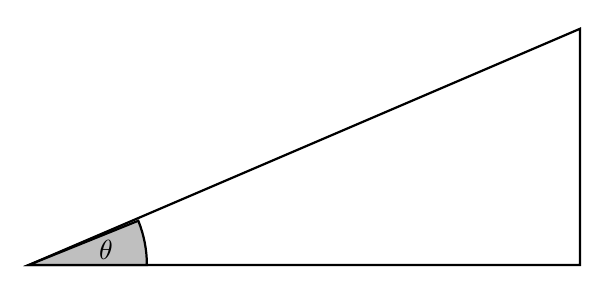
\begin{tikzpicture}[thick]
\coordinate (O) at (0,0);
\coordinate (A) at (7,0);
\coordinate (B) at (7,3);
\draw (O)--(A)--(B)--cycle;

%\tkzLabelSegment[below=2pt](O,A){\textit{adjacent leg}}
%\tkzLabelSegment[left=2pt](O,B){\textit{hypotenuse}}
%\tkzLabelSegment[above right=2pt](A,B){\textit{opposite leg}}

\tkzLabelSegment[below=5pt](O,A){\textit{x}}
\tkzLabelSegment[above left=5pt](O,B){\textit{r}}
\tkzLabelSegment[right=5pt](A,B){\textit{y}}

%\tkzMarkAngle[fill= orange,size=1.5cm, opacity=.4](A,O,B)
%\tkzLabelAngle[pos = 2](A,O,B){\texttt{$\theta$}}
 %%% AAAARGH ovan slutade funka så gjorde nedan HACK i stället
 \draw[fill=lightgray, thick] (0,0) -- (0:1.5cm) arc (0:22:1.5cm) node at (11:1.0cm) {$\theta$} -- cycle;

% \tkzMarkAngle[fill= orange,size=0.65cm, opacity=.4](A,O,B)
% \tkzLabelAngle[pos = 0.35](A,O,B){$\gamma$}
%
% \tkzMarkAngle[fill= orange,size=0.8cm, opacity=.4](B,A,O)
% \tkzLabelAngle[pos = 0.6](B,A,O){$\alpha$}
%
% \tkzMarkAngle[fill= orange,size=0.7cm, opacity=.4](O,B,A)
% \tkzLabelAngle[pos = 0.5](O,B,A){$\beta$}

\end{tikzpicture}

\item Du har nytta av metoderna \code{math.cos(theta)} och \code{math.sin(theta)} vid omvandling från polära koordinater.

\item Notera att klassens attribut är av typen \code{Double} och inte \code{Int}, trots att vi senare ska använda punkten för att beskriva en diskret pixelposition i ett \code{PixelWindow}. Anledningen till detta är att det kan uppstå avrundningsfel vid numeriska beräkningar. Detta blir särskilt märkbart vid upprepad räkning med små värden, t.ex. när man ritar en approximerad cirkel med många linjesegment.
\end{itemize}

\Subtask Klassen \code{PolygonWindow} nedan innehåller ett \code{PixelWindow} och ger möjlighet att rita ut polygoner. 
Kopiera koden för \code{PolygonWindow} till en ny kodfil \code{PolygonWindow.scala} i samma katalog som du placerade \code{Point} ovan i.

\begin{Code}
//> using dep "se.lth.cs::introprog:1.4.0"
package graphics

import introprog.PixelWindow
import java.awt.Color

extension def toPixels(p: Point): Seq[Int] = 
  Seq(point.x.round.toInt, point.y.round.toInt)

class PolygonWindow:
  val black     = Color(0,0,0)
  val coolGreen = Color(0,255,111)
  val width     = 500
  val height    = 500

  val window = 
    PixelWindow(width, height,  title = "Polygons", 
                background = black, foreground = coolGreen)

  def draw(polygon: Polygon): Unit =
    for i <- 0 until polygon.nbrOfCorners do
      val from = polygon.points(i).toPixels.map(_ + width / 2)
      val mod = polygon.points((i+1) % polygon.nbrOfCorners)
      val to = mod.toPixels.map(_ + width / 2)
      window.line(from(0), from(1), to(0), to(1), lineWidth = 2)
\end{Code}

Skapa en case-klass vid namn \code{Polygon} men en parameter \code{points: Vector[Point]} och ett attribut \code{val nbrOfCorners: Int}. Case-klassen \code{Polygon} ska också ligga i paketet \code{graphics}. 

Likt klassen \code{Point} ovan ska också \code{Polygon} ha ett kompanjonsobjekt. 
Kompanjonsobjektet ska ha en metod som skapar en regelbunden polygon vid namn \code{regular} med följande parametrar: \code{nbrOfCorners: Int, radius: Double, midPoint: Point}\\
Fundera över hur case-klassen \code{Polygon} och dess kompanjonsobjekt ska se ut för att koden ovan i \code{PolygonWindow} ska fungera som tänkt. Testa att allt fungerar i REPL.

\Subtask Kan man använda metoden \code{regularPolygon} för att rita cirklar? Kan man använda \code{Polygon} för att representera oregelbundna polygoner?
Testa i REPL.

\SOLUTION

\TaskSolved \what~

\Subtask \begin{Code}
package graphics

case class Point(x: Double, y: Double):
  val r: Double = math.hypot(x, y)
  val theta: Double = math.atan2(y, x)
  def +(p: Point): Point = Point(x + p.x, y + p.y)

object Point:
  def polar(r: Double, theta: Double): Point =
    Point(r * math.cos(theta), r * math.sin(theta))
\end{Code}

\Subtask \begin{Code}
package graphics

case class Polygon(points: Vector[Point]):
  val nbrOfCorners: Int = points.length
  
object Polygon:
  def regular(nbrOfCorners: Int, radius: Double, midPoint: Point): Polygon =
    val points = new Array[Point](nbrOfCorners)
    for i <- 0 until nbrOfCorners do
      val theta = i * (2 * math.Pi) / nbrOfCorners
      points(i) = Point.polar(radius, theta) + midPoint
    end for
    Polygon(points.toVector)
\end{Code}

\Subtask 
En perfekt cirkel går inte att skapa, men det går att komma tillräckligt nära för att göra det omöjligt att se hörnen.
Testa till exempel med 50 hörn likt nedan.
\begin{REPL}
scala> import graphics.*
scala> val circle = Polygon.regular(50,70,Point(-25,-25))
scala> val window = PolygonWindow()
scala> window.draw(circle)
\end{REPL}

Även en oregelbunden polygon går att skapa. Använd då konstruktorn till \code{Polygon} direkt. Till exempel likt nedan.
\begin{REPL}
scala> val irregular = 
         Polygon(Vector(Point(34,83), Point(16,42), Point(77,77), Point(100,138)))
scala> window.draw(irregular)
\end{REPL}

\QUESTEND




\WHAT{Klasser, instanser och skräp.}

\QUESTBEGIN

\Task  \what~För länge sedan i en galax långt långt borta...

\begin{Code}
case class Arm(ärTillVänster: Boolean)

case class Ben(ärTillVänster: Boolean)

case class Huvud(harHår: Boolean = true)

case class Rymdvarelse(
      arm1:   Arm   = Arm(true),
      arm2:   Arm   = Arm(false),
      ben1:   Ben   = Ben(true),
      ben2:   Ben   = Ben(false),
      huvud1: Huvud = Huvud(harHår = false),
  var huvud2: Huvud = Huvud()
):
  def ärSkallig = !huvud1.harHår && !huvud2.harHår
\end{Code}

\Subtask Klistra in ovan rymdkod i REPL och evaluera nedan rader. Rita minnessituationen efter rad 5 och beskriv vad som händer.
\begin{REPL}
scala> val alien = Rymdvarelse()
scala> alien.ärSkallig
scala> val predator = Rymdvarelse()
scala> predator.ärSkallig
scala> predator.huvud2 = alien.huvud1
scala> predator.huvud2 eq alien.huvud1  // test av referenslikhet
scala> println(predator)
scala> predator.ärSkallig
\end{REPL}

\Subtask Vad händer så småningom med det ursprungliga \code{huvud2}-objektet i predator efter tilldelningen på rad 5? Går det att referera till detta objekt på något sätt?

\SOLUTION

\TaskSolved \what

\SubtaskSolved  Vi skapar två rymdvarelser, \code{alien} och \code{predator}, med vardera två ben och två armar, samt vardera två huvuden (där det ena är skalligt och det andra har hår). Efter det är varken \code{alien} eller \code{predator} skallig eftersom båda har ett huvud med hår. Sen låter man referensen till \code{predator}s huvud med hår referera till aliens huvud utan hår. Nu är predator helt skallig och delar huvud med alien.

\includegraphics[scale=0.65]{../img/w06-solutions/2b}

\SubtaskSolved  Eftersom det inte längre finns någon referens som pekar på det objektet kommer skräpsamlaren att ta hand om det och det kommer förr eller senare skrivas över av något annat när platsen i minnet behövs. Objekt som inte har någon referens till sig går inte att komma åt.

\QUESTEND




\WHAT{Case-klass. Oföränderlig kvadrat.}

\QUESTBEGIN

\Task \label{task:Square} \what~

\Subtask Implementera nedan kvadrat med en editor och klistra in den i REPL.

\begin{Code}
case class Square(val x: Int = 0, val y: Int = 0, val side: Int = 1):
  val area: Int = ???

  /** Creates a new Square moved to position (x + dx, y + dy) */
  def moved(dx: Int, dy: Int): Square = ???

  def isEqualSizeAs(that: Square): Boolean = ???

  /** Multiplies the side with factor and rounded to nearest integer */
  def scale(factor: Double): Square = ???

object Square:
  /** A Square at (0, 0) with side 1 */
  val unit: Square = ???
\end{Code}

\Subtask Testa din kvadrat enligt nedan. Förklara vad som händer.

\begin{REPL}
scala> val (s1, s2) = (Square(), Square(1, 10, 1))
scala> val s3 = s1 moved (1,-5)
scala> s1 isEqualSizeAs s3
scala> s2 isEqualSizeAs s1
scala> s1 isEqualSizeAs Square.unit
scala> s2.scale(math.Pi) isEqualSizeAs s2
scala> s2.scale(math.Pi) isEqualSizeAs s2.scale(math.Pi)
scala> s2.scale(math.Pi) eq s2.scale(math.Pi)
scala> Square.unit eq Square.unit
\end{REPL}

\SOLUTION

\TaskSolved \what

\SubtaskSolved

\begin{Code}
case class Square(val x: Int = 0, val y: Int = 0, val side: Int = 1):
  val area: Int = side * side

  def moved(dx: Int, dy: Int): Square = Square(x + dx, y + dy, side)

  def isEqualSizeAs(that: Square): Boolean = this.side == that.side

  def scale(factor: Double): Square =
    Square(x, y, (side * factor).round.toInt)

object Square:
  val unit: Square = Square()
\end{Code}

\SubtaskSolved
\begin{REPL}
scala> val (s1, s2) = (Square(), Square(1, 10, 1))
val s1: Square = Square(0,0,1)
val s2: Square = Square(1,10,1)

scala> val s3 = s1 moved (1,-5)
val s3: Square = Square(1,-5,1)

scala> s1 isEqualSizeAs s3       // lika storlek
val res0: Boolean = true

scala> s2 isEqualSizeAs s1       // lika storlek
val res1: Boolean = true

scala> s1 isEqualSizeAs Square.unit   // s1 har sidan 1
val res2: Boolean = true

scala> s2.scale(math.Pi) isEqualSizeAs s2  // olika storlek
val res3: Boolean = false

scala> s2.scale(math.Pi) == s2.scale(math.Pi) // lika innehåll
val res4: Boolean = true

scala> s2.scale(math.Pi) eq s2.scale(math.Pi)  // olika objekt
val res5: Boolean = false

scala> Square.unit eq Square.unit   // samma objekt
val res6: Boolean = true
\end{REPL}

\QUESTEND




\clearpage

\AdvancedTasks %%%%%%%%%%%%%%%%%%%%%%%%%%%%%%%%%%%%%%%%%%%%%%%%%%%%%%%%%%%%%%%%%

\WHAT{Innehållslikhet mellan olika typer.}

\QUESTBEGIN

\Task \what~Klistra in nedan klasser i REPL och undersök vad som händer.

\begin{Code}
class Gurka(val vikt: Int)

class Bil(val typ: String)
\end{Code}

\begin{REPL}
scala> class Gurka(val vikt: Int)
     |
     | class Bil(val typ: String)
// defined class Gurka
// defined class Bil

scala> 42 == "Fyrtiotvå"

scala> Gurka(50) == Bil("Sedan")

\end{REPL}

Finns det något resultat som är problematiskt, och i så fall, varför?


\SOLUTION

\TaskSolved \what~
\begin{REPL}
scala> 42 == "Fyrtiotvå"
1 |42 == "Fyrtiotvå"
  |^^^^^^^^^^^^^^^^^
  |Values of types Int and String cannot be compared with == or !=

scala> Gurka(50) == Bil("Sedan")
val res0: Boolean = false
\end{REPL}

Det andra uttrycket är problematiskt eftersom det alltid kommer resultera i \code|false|, då klasserna \code|Gurka| och \code|Bil| är två ojämförbara typer som inte bör jämföras med avseende på innehållslikhet. Detta försämrar typsäkerheten vilket ökar risken för svårupptäckta buggar där fel typer jämförs.

Likhetsjämförelser som sker mellan primitiva typer typkollas av kompilatorn och kan därför ge kompileringsfel om två olika typer, såsom \code|Int| och \code|String|, jämförs med varandra. Detta gäller dock i regel inte egendefinierade typer, vilket alltså innebär att en likhetsjämförelse mellan olika egendefinierade typer alltid resulterar i \code|false|.

Det är emellertid möjligt att få samma typkoll för egendefinierade typer som för primitiva typer genom att importera \code|scala.language.strictEquality|.

\begin{Code}
import scala.language.strictEquality
class Gurka(val vikt: Int)

class Bil(val typ: String)
\end{Code}

\begin{REPL}
scala> Gurka(50) == Bil("Sedan")
1 |Gurka(50) == Bil("Sedan")
  |^^^^^^^^^^^^^^^^^^^^^^^^^
  |Values of types Gurka and Bil cannot be compared with == or !=
\end{REPL}

\QUESTEND


\WHAT{Attributrepresentation. Privat konstruktor. Fabriksmetod.}

\QUESTBEGIN

\Task \what~Kim Kodkunnig skapade för länge sedan denna klass som används på många ställen i befintlig kod:

\begin{Code}
class Point private (val x: Int, val y: Int)
object Point:
  def apply(x: Int = 0, y: Int = 0): Point = new Point(x, y)
  val origo = apply()
\end{Code}

\Subtask Vad händer om du försöker instansiera Kim Kodkunnigs klass direkt med nyckelordet \code{new}?

\Subtask Varför använder Kim Kodkunnig ett kompanjonsobjekt med en fabriksmetod? Vilka accessregler gäller mellan ett kompanjonsobjekt och klassen med samma namn?

\Subtask Hjälp Kim Kodkunnig att ändra attributrepresentationen så att det oföränderliga tillståndet utgörs av en 2-tupel \code{val p: (Int, Int)} i stället. Befintlig kod ska inte behöva ändras och klassen \code{Point} ska bete sig från ''utsidan'' precis som innan.

\SOLUTION

\TaskSolved \what~

\SubtaskSolved Det blir kompileringsfel eftersom konstruktorn är privat.
\begin{REPL}
scala> class Point private (val x: Int, val y: Int)
     | object Point:
     |   def apply(x: Int = 0, y: Int = 0): Point = new Point(x, y)
     |   val origo = apply()
     |
// defined class Point
// defined object Point

scala> new Point(0, 0)
1 |new Point(0, 0)
  |    ^^^^^
  |constructor Point cannot be accessed as a member of Point from module class
\end{REPL}

\SubtaskSolved
\begin{itemize}
  \item Genom att ha en privat konstruktor och bara göra indirekt instansiering via fabriksmetod är lätt ändra attributrepresentation i framtiden utan att befintlig kod behöver ändras.

  \item Accessreglerna för kompanjonsobjekt är sådana att kompanjoner ser varandras privata delar.
\end{itemize}

\SubtaskSolved

\begin{Code}
class Point private (private val p: (Int, Int)):
  def x: Int = p._1
  def y: Int = p._2

object Point:
  def apply(x: Int = 0, y: Int = 0): Point = new Point(x, y)
  val origo = apply()
\end{Code}

\QUESTEND



\WHAT{Synlighet av klassparametrar och konstruktor, \code{private[this]}.}

\QUESTBEGIN

\Task  \what~

\Subtask En av gurk-klasserna nedan är trasig. Varför och vad blir det för fel?

\begin{Code}
class Gurka1(vikt: Int)

class Gurka2(val vikt: Int)

class Gurka3(private val vikt: Int)

class Gurka4(private val vikt: Int, kompis: Gurka4):
  def kompisVikt = kompis.vikt

class Gurka5(private[this] val vikt: Int, kompis: Gurka5):
  def kompisVikt = kompis.vikt

class Gurka6 private (vikt: Int)

class Gurka7 private (var vikt: Int)
object Gurka7:
  def apply(vikt: Int) =
    require(vikt >= 0, "negativ vikt: " + vikt)
    new Gurka7(vikt)
\end{Code}

\Subtask Undersök nedan vad nyckelorden \code{val} och \code{private} får för konsekvenser. Förklara vad som händer. Vilka rader ger vilka felmeddelanden?

\begin{REPL}
scala> new Gurka1(42).vikt
scala> new Gurka2(42).vikt
scala> new Gurka3(42).vikt
scala> val ingenGurka: Gurka4 = null
scala> new Gurka4(42, ingenGurka).kompisVikt
scala> new Gurka4(42, new Gurka4(84, null)).kompisVikt
scala> new Gurka6(42)
scala> new Gurka7(-42)
scala> Gurka7(-42)
scala> val g = Gurka7(42)
scala> g.vikt
scala> g.vikt = -1
scala> g.vikt
\end{REPL}


\SOLUTION


\TaskSolved \what

\SubtaskSolved \code{Gurka5} är trasig. Eftersom vikten i \code{Gurka5} är privat för instansen och inte klassen, kan en instans inte accessa en annan instans vikt.
\begin{REPL}
11 |  def kompisVikt = kompis.vikt
   |                   ^^^^^^^^^^^
   |value vikt cannot be accessed as a member of (Gurka5.this.kompis : Gurka5) from class Gurka5.
\end{REPL}


\SubtaskSolved
\begin{REPL}
scala> new Gurka1(42).vikt
1 |new Gurka1(42).vikt
  |^^^^^^^^^^^^^^^^^^^
  |value vikt cannot be accessed as a member of Gurka1 from module class

scala> new Gurka2(42).vikt
val res0: Int = 42

scala> new Gurka3(42).vikt
1 |new Gurka3(42).vikt
  |^^^^^^^^^^^^^^^^^^^
  |value vikt cannot be accessed as a member of Gurka3 from module class

scala> val ingenGurka: Gurka4 = null
val ingenGurka: Gurka4 = null

scala> new Gurka4(42, ingenGurka).kompisVikt
java.lang.NullPointerException: Cannot invoke "rs$line$1$Gurka4.vikt()" bec...
  at rs$line$1$Gurka4.kompisVikt(rs$line$1:8)
  ... 38 elided

scala> new Gurka4(42, new Gurka4(84, null)).kompisVikt
val res2: Int = 84

scala> new Gurka6(42)
1 |new Gurka6(42)
  |    ^^^^^^
  |constructor Gurka6 cannot be accessed as a member of Gurka6 from module...

scala> new Gurka7(-42)
1 |new Gurka7(-42)
  |    ^^^^^^
  |constructor Gurka7 cannot be accessed as a member of Gurka7 from module...

scala> Gurka7(-42)
java.lang.IllegalArgumentException: requirement failed: negativ vikt: -42

scala> val g = Gurka7(42)
val g: Gurka7 = Gurka7@51fd1c7c

scala> g.vikt
val res4: Int = 42

scala> g.vikt = -1

scala> g.vikt
val res5: Int = -1
\end{REPL}

\QUESTEND





\WHAT{Egendefinierad setter kombinerat med privat konstruktor.}

\QUESTBEGIN

\Task  \what~Klistra in denna kod i REPL:

\begin{Code}
class Gurka8 private (private var _vikt: Int):
  def vikt = _vikt
  def vikt_=(v: Int): Unit =
    require(v >= 0, "negativ vikt: " +v)
    _vikt = v

object Gurka8:
  def apply(vikt: Int) =
    require(vikt >= 0, "negativ vikt: " + vikt)
    new Gurka8(vikt)
\end{Code}


\Subtask Förklara vad som händer nedan. Vilka rader ger vilka felmeddelanden?
\begin{REPL}
scala> val g = Gurka8(-42)
scala> val g = Gurka8(42)
scala> g.vikt
scala> g.vikt = 0
scala> g.vikt = -1
scala> g.vikt += 42
scala> g.vikt -= 1000
\end{REPL}

\Subtask Vad är fördelen med möjligheten att skapa egendefinierade setters?

\SOLUTION


\TaskSolved \what


\SubtaskSolved

Rad 1:
\begin{REPL}
	java.lang.IllegalArgumentException: requirement failed: negativ vikt: -42
\end{REPL}
\code{Gurka8.apply} kräver att \code{vikt >= 0} annars kastar \code{require} ett undantag.

Rad 5:
\begin{REPL}
	java.lang.IllegalArgumentException: requirement failed: negativ vikt: -1
\end{REPL}
Settern \code{vikt_=} kräver att \code{vikt >= 0} annars kastar \code{require} ett undantag.

Rad 7:
\begin{REPL}
	java.lang.IllegalArgumentException: requirement failed: negativ vikt: -958
\end{REPL}
Eftersom \code{42 - 1000} är mindre än noll kastar \code{require} ett undantag.

\SubtaskSolved  Man kan sätta egna mer specifika krav på vad som får göras med värdena så man har större koll på att inget oväntat händer.

\QUESTEND




\WHAT{Objekt med föränderligt tillstånd \Eng{mutable state}.}

\QUESTBEGIN

\Task  \what~  Du ska implementera en modell av en hoppande groda som uppfyller följande krav:
\begin{enumerate}%[nolistsep, noitemsep]
\item Varje grodobjekt ska hålla reda på var den är.
\item Varje grodobjekt ska hålla reda på hur långt grodan hoppat totalt.
\item Varje grodobjekt ska kunna beräkna hur långt det är mellan grodans nuvarande position och utgångsläget.
\item Alla grodor börjar sitt hoppande i origo.
\item En groda kan hoppa enligt två metoder:
  \begin{itemize} [nolistsep, noitemsep]
  \item relativ förflyttning enligt parametrarna \code{dx} och \code{dy},
  \item slumpmässig relativ förflyttning $[1, 10]$ i x-ledsförändring och $[1, 10]$ i y-ledsförändring.
  \end{itemize}
\end{enumerate}

\Subtask Implementera klassen \code{Frog} enligt nedan kodskelett och ovan krav.

\begin{Code}
class Frog private (initX: Int = 0, initY: Int = 0):
  def x: Int = ???
  def y: Int = ???

  def jump(dx: Int, dy: Int): Unit = ???
  def randomJump: Unit = ???

  def distanceToStart: Double = ???
  def distanceJumped: Double = ???
  def distanceTo(that: Frog): Double = ???

object Frog:
  def spawn(): Frog = ???
\end{Code}
\emph{Tips:}
\begin{itemize} [nolistsep, noitemsep]
\item Om namnet man vill ge ett privat föränderligt attribut ''krockar'' med ett metodnamn, är det vanligt att man börjar attributets namn med understreck, t.ex. \code{private var _x } för att på så sätt undkomma namnkonflikten.
\item Inför en metod i taget och klistra in den nya grodan i REPL efter varje utvidgning och testa.
\end{itemize}



\Subtask Skapa en metod \code{def test(): Unit} i ett singelobjekt \code{FrogTest} som innehåller kod som gör minst en kontroll av varje krav. Om ingen kontroll går fel ska \code{"Test Ok!"} skrivas ut, annars ska exekveringen avbrytas. \emph{Tips:} Använd \code{assert(b, msg)} som avbryter exekveringen och skriver ut \code{msg} om \code{b} är falsk.

\Subtask Vad kallas en metod som enbart returnerar värdet av ett privat attribut?

\Subtask Inför setters för attributen som håller reda på x- och y-postitionen. Förändringar av positionen i x- eller y-led ska räknas som ett hopp och alltså registreras i det attribut som håller reda på det ackumulerade hoppavståndet.

\Subtask Simulera ett massivt grodhoppande med krockdetektering genom att skapa 100 grodor som till att börja med är placerade på x-axeln med avståndet $8$ längdenheter mellan sig. För varje runda i en \code{while}-sats, låt en slumpässigt vald groda göra ett \code{randomJump} tills någon groda befinner sig närmare än $0.5$ längdenheter, vilket är definitionen på att de har krockat. Räkna hur många looprundor som behövs innan något grodpar krockar och skriv ut antalet. Skriv även ut det totala antalet \\ \emph{Tips:} Börja med pseudokod på papper. Använd en grodvektor.


\SOLUTION


\TaskSolved \what


\SubtaskSolved
\begin{Code}
class Frog private (initX: Int = 0, initY: Int = 0):
  private var _x: Int = initX
  private var _y: Int = initY
  private var _distanceJumped: Double = 0

  def x: Int = _x
  def y: Int = _y

  def jump(dx: Int, dy: Int): Unit =
    _x += dx
    _y += dy
    _distanceJumped += math.hypot(dx, dy)


  def randomJump: Unit =
    def rnd = util.Random.nextInt(10) + 1
    jump(rnd, rnd)

  def distanceToStart: Double = math.hypot(x,y)
  def distanceJumped: Double = _distanceJumped
  def distanceTo(f: Frog): Double = math.hypot(x - f.x, y - f.y)

object Frog:
  def spawn(): Frog = Frog()
\end{Code}

\SubtaskSolved Exempel på testprogram:
\begin{Code}
object FrogTest:
  def test(): Unit =
    val f1 = Frog.spawn()
    assert(f1.x == 0 && f1.y == 0, "Test of spawn, reqt 1 & 4 failed.")

    f1.jump(4, 3)
    assert(f1.x == 4 && f1.y == 3, "Test of jump, reqt 1 & 4 failed.")

    f1.jump(4, 3)
    assert(f1.distanceJumped == 10, "Test of jump, reqt 2 failed.")

    f1.jump(-4, -3)
    assert(f1.distanceToStart == 5, "Test of jump, reqt 3 failed.")

    for x <- 1 to 10000 do
      val f2 = Frog.spawn()
      f2.randomJump
      assert(f2.x > 0 && f2.x <= 10 && f2.y > 0 && f2.y <= 10,
        "Test of randomJump, reqt 5 failed.")

    println("Test Ok!")
\end{Code}

\SubtaskSolved  En metod som är en indirekt avläsning av attributvärden kallas getter.

\SubtaskSolved
\begin{Code}
class Frog private (initX: Int = 0, initY: Int = 0):
  private var _x: Int = initX
  private var _y: Int = initY
  private var _distanceJumped: Double = 0

  def jump(dx: Int, dy: Int): Unit =
    _x += dx
    _y += dy
    _distanceJumped += math.hypot(dx, dy)

  def x: Int = _x
  def x_=(newX: Int): Unit = // Setter för x
    _distanceJumped += math.abs(x - newX)
    _x = newX

  def y: Int = _y
  def y_=(newY: Int): Unit = // Setter för y
    _distanceJumped += math.abs(y - newY)
    _y = newY


  def randomJump: Unit =
    def rnd = util.Random.nextInt(10) + 1
    jump(rnd, rnd)

  def distanceToStart: Double = math.hypot(x,y)
  def distanceJumped: Double = _distanceJumped
  def distanceTo(f: Frog): Double = math.hypot(x - f.x, y - f.y)

object Frog:
  def spawn(): Frog = Frog()
\end{Code}

\SubtaskSolved
\begin{Code}
object FrogSimulation:
  def isAnyCollision(frogs: Vector[Frog]): Boolean =
    var found = false
    frogs.indices.foreach(i =>  // generate all pairs (i,j)
      for j <- i + 1 until frogs.size do
        if !found then
          found = frogs(i).distanceTo(frogs(j)) <= 0.5
    )
    found

  def jumpUntilCrash(n: Int = 100, initDist: Int = 8): (Int, Double) =
    val frogs = Vector.fill(n)(Frog.spawn())
    (0 until n).foreach(i => frogs(i).x = i * initDist)
    var count = 0
    while !isAnyCollision(frogs) do
      frogs(util.Random.nextInt(n)).randomJump
      count += 1
    (count, frogs.map(_.distanceJumped).sum)


  def run(nbrOfCrashTests: Int = 10) =
    for i <- 1 to nbrOfCrashTests do
      val (n, dist) = jumpUntilCrash()
      println(s"\nAntalet looprundor innan grodkrock: $n")
      println(s"Totalt avstånd hoppat av alla grodor: $dist")
\end{Code}

\QUESTEND




\QUESTBEGIN

\Task  \what~  Webbshoppen \textbf{UberSquare} säljer flyttbara kvadrater. I affärsmodellen ingår att ta betalt per förflyttning. Du ska hjälpa UberSquare att utveckla en enkel prototyp för att imponera på riskkapitalister. (En variant av denna uppgift ingick i tentamen 2017-08-23.)

\Subtask Implementera \code{Square} enligt dokumentationskommentarerna i efterföljande kodskiss och enligt dessa krav:

\begin{enumerate}%[nolistsep, noitemsep]
   \item Varje instans av \code{Square} ska räkna antalet förflyttningar som gjorts sedan instansen konstruerats.

   \item För att kunna övervaka sina kunder vill UberSquare även räkna det totala antalet förflyttningar som gjorts av alla kvadrater som någonsin skapats (s.k. \emph{big data}).

  \item Varje gång förflyttning sker ska ett visst belopp adderas till den ackumulerade kostnaden för respektive kvadrat, enligt kostnadsberäkningen i krav 4.

  \item UberSquare är oroliga för att kvadraterna flyttas för långt bort och bestämmer därför att för varje förflyttning ska den ackumulerade kvadratkostnaden ökas med den nya positionens avstånd till ursprungsläget vid kvadratens konstruktion multiplicerat med aktuell storlek på kvadraten.

  \item För att framstå som goda berättar UberSquare i sin marknadsföring att det är gratis att skala kvadrater. \footnote{D.v.s. ett anrop av metoden \code{scale} orsakar ingen omedelbar kostnad.}
\end{enumerate}

\begin{CodeSmall}
/** A mutable and expensive Square. */
class Square private (val initX: Int, val initY: Int, val initSide: Int):
  private var nMoves = 0
  private var sumCost = 0.0

  private var _x = initX
  private var _y = initY

  private var _side = initSide

  private def addCost(): Unit =
    sumCost += ???

  def x: Int = ???
  def y: Int = ???

  def side = ???

  /** Scales the side of this square and rounds it to nearest integer */
  def scale(factor: Double): Unit = ???

  /** Moves this square to position (x + xd, y + dy) */
  def move(dx: Int, dy: Int): Unit = ???

  /** Moves this square to position (x, y) */
  def moveTo(x: Int, y: Int): Unit = ???

  /** The accumulated cost of this Square */
  def cost: Double = ???

  /** Returns the accumulated cost. Sets the accumulated cost to zero. */
  def pay: Double = ???

  override def toString: String =
    s"Square[($x, $y), side: $side, #moves: $nMoves times, cost: $sumCost]"


object Square:
  private var created = Vector[Square]()

  /** Constructs a new Square object at (x, y) with size side */
  def apply(x: Int, y: Int, side: Int): Square =
    require(side >= 0, s"side must be positive: $side")
    ???

  /** Constructs a new Square object at (0, 0) with side 1 */
  def apply(): Square = ???

  /** The total number of moves that have been made for all squares. */
  def totalNumberOfMoves: Int = ???

  /** The total cost of all squares. */
  def totalCost: Double = ???
\end{CodeSmall}

\Subtask Testa din kvadratprototyp i REPL. Använd t.ex. koden nedan:
\begin{REPL}
scala> val xs = Vector.fill(10)(Square())
scala> xs.foreach(_.move(2, 3))
scala> xs.foreach(_.scale(2.9))
scala> val (m, c) = (Square.totalNumberOfMoves, Square.totalCost)
val m: Int = 10
val c: Double = 36.055512754639885
\end{REPL}

\SOLUTION

\TaskSolved \what~

\begin{CodeSmall}
class Square private (val initX: Int, val initY: Int, val initSide: Int):
  private var nMoves = 0
  private var sumCost = 0.0

  private var _x = initX
  private var _y = initY

  private var _side = initSide

  private def addCost(): Unit =
    sumCost += math.hypot(x - initX, y - initY) * side

  def x: Int = _x
  def y: Int = _y

  def side = _side

  def scale(factor: Double): Unit = _side = (_side * factor).round.toInt

  def move(dx: Int, dy: Int): Unit =
    _x += dx; _y += dy
    nMoves += 1
    addCost()

  def moveTo(x: Int, y: Int): Unit =
    _x = x; _y = y
    nMoves += 1
    addCost()

  def cost: Double = sumCost

  def pay: Double = {val temp = sumCost; sumCost = 0; temp}

  override def toString: String =
    s"Square[($x, $y), side: $side, #moves: $nMoves times, cost: $sumCost]"

object Square:
  private var created = Vector[Square]()

  def apply(x: Int, y: Int, side: Int): Square =
    require(side >= 0, s"side must be positive: $side")
    val sq = (new Square(x, y, side))
    created :+= sq
    sq

  def apply(): Square = apply(0, 0, 1)

  def totalNumberOfMoves: Int = created.map(_.nMoves).sum

  def totalCost: Double = created.map(_.cost).sum
\end{CodeSmall}

\QUESTEND



\WHAT{Hjälpkonstruktor.}

\QUESTBEGIN

\Task\Uberkurs \label{task:aux-constructor} \what~I tidigare uppgifter har vi möjliggjort alternativa sätt att skapa instanser genom default-argument och fabriksmetoder i kompanjonsobjekt.

Ett annat sätt att göras detta på, som i Scala är ovanligt\footnote{Men i Java är detta mycket vanligt då defaultargument m.m. inte ingår i språket.}, är att definiera flera konstruktorer inne i klasskroppen. I Scala kallas en sådan extra konstruktor för \textbf{hjälpkonstruktor} \Eng{auxiliary constructor}.

En hjälpkonstruktor skapar man i Scala genom att definiera en metod som har det speciella namnet \code{this}, alltså en deklaration \code{def this(...) = ...} Hjälpkonstruktorer måste börja med att anropa en annan konstruktor, antingen den primära konstruktorn (d.v.s. den som klasshuvudet definierar) eller en tidigare definierad  hjälpkonstruktor.

\Subtask Läs mer om hjälpkonstruktorer här: \\ \href{http://www.artima.com/pins1ed/functional-objects.html#6.7}{www.artima.com/pins1ed/functional-objects.html\#6.7}

\Subtask Hitta på en egen uppgift med hjälpkonstruktorer, baserat på någon av klasserna i tidigare övningar.


%\Task \TODO \\ \code{class Rational private (numerator: BigInt, denominator: BigInt)} \\
%Inspirerat av Rational i pins1ed med GCD\SOLUTION

\QUESTEND

%!TEX encoding = UTF-8 Unicode
%!TEX root = ../compendium1.tex

% INGEN LAB DENNA VECKA

\Lab{\LabWeekFIVE}

\begin{Preparations}
\item \DoExercise{\ExeWeekFIVE}{05}.
\item Du har två veckor på dig att göra \texttt{blockbattle}. Läs redan nu igenom alla uppgifter i avsnitt \ref{section:lab:\LabWeekSIX}, men gör först  grundövningarna innan du påbörjar labben, speciellt uppgift \ref{exe:classes:labprep} i avsnitt \ref{section:exe:\ExeWeekFIVE}.
\end{Preparations}



\input{modules/w06-patterns-chapter.tex}
%\input{generated/w06-chaphead-generated.tex}

%!TEX encoding = UTF-8 Unicode
%!TEX root = ../exercises.tex

\ifPreSolution



\Exercise{\ExeWeekSIX}\label{exe:W06}

\begin{Goals}
\item Kunna skapa och använda \code{match}-uttryck med konstanta värden, garder och mönstermatchning med case-klasser.
\item Kunna skapa och använda case-objekt för matchningar på uppräknade värden.
\item Kunna hantera saknade värden med hjälp av typen \code{Option} och mönstermatchning på \code{Some} och \code{None}.
\item Kunna fånga undantag med \code{scala.util.Try}.
\item Känna till \code{try}, \code{catch} och \code{throw}.
%\item Känna till \jcode{switch}-satser i Java.
\item Känna till nyckelordet \code{sealed} och förstå nyttan med förseglade typer.
%\item Känna till relationen mellan \code{hashCode} och \code{equals}.
%\item Kunna skapa partiella funktioner med case-uttryck.
%\item Känna till betydelsen av små och stora begynnelsebokstäver i case-grenar i en matchning, samt förstå hur namn binds till värden in en case-gren.
%\item Kunna använda \code{flatMap} tillsammans med \code{Option} och \code{Try}.
%\item Känna till skillnaderna mellan \code{try}-\code{catch} i Scala och java.
%\item Känna till att metoden \code{unapply} används vid mönstermatchning.
%\item Kunna implementera \code{equals} med hjälp av en \code{match}-sats, som fungerar för finala klasser utan arv.
%\item Känna till \code{null}.
\end{Goals}

\begin{Preparations}
\item \StudyTheory{06}
\end{Preparations}

\BasicTasks %%%%%%%%%%%%%%%%

\else



\ExerciseSolution{\ExeWeekSIX}

\BasicTasks %%%%%%%%%%%

\fi




\WHAT{Matcha på konstanta värden.}

\QUESTBEGIN

\Task \label{task:vegomatch} \what~   % I Scala finns ingen \jcode{switch}-sats. I stället har Scala ett \code{match}-uttryck som är mer kraftfullt. Dock saknar Scala nyckelordet \jcode{break} och Scalas \code{match}-uttryck kan inte ''falla igenom'' som skedde i uppgift \ref{task:switch}\ref{subtask:break}.

\Subtask \label{subtask:vegomatch} Skriv nedan program med en kodeditor och spara i filen \texttt{Match.scala}. Kompilera och kör och och ge som argument din favoritgrönsak. Vad händer? Förklara hur ett \code{match}-uttryck fungerar.

\scalainputlisting[numbers=left,basicstyle=\ttfamily\fontsize{11}{12}\selectfont]{examples/Match.scala}

\Subtask Vad blir det för felmeddelande om du tar bort case-grenen för defaultvärden och indata väljs så att inga case-grenar matchar? Är det ett exekveringsfel eller ett kompileringsfel?

% \Subtask Beskriv några skillnader i syntax och semantik mellan Javas flervalssats \jcode{switch} och Scalas flervalsuttryck \code{match}.



\SOLUTION


\TaskSolved \what


\SubtaskSolved  %Svaret blir identiskt mot föregående uppgiften i Java.\\
Scalas \code{match}-uttryck jämför stegvis värdet med varje \code{case} för att sedan returnera ett värde tillhörande motsvarande \code{case}.

\SubtaskSolved  \begin{REPL}
scala.MatchError 
\end{REPL}
Exekveringsfel, uppstår av en viss input under körningen.

% \SubtaskSolved  Scalas \code{match} ersätter kolonet (:) i \jcode{switch} med Scalas högerpil (=>).\\
% \code{match} returnerar ett värde till skillnad från \jcode{switch} som inte returnerar något.\\
% \code{match} kan inte $"$falla igenom$"$ så ett \jcode{break} efter varje \jcode{case} är inte nödvändigt.\\
% Till skillnad från \jcode{switch}-satsen kastar \code{match} ett \code{MatchError} om ingen matchning skulle ske.



\QUESTEND






\WHAT{Gard i case-grenar.}

\QUESTBEGIN

\Task  \what~  Med hjälp en gard \Eng{guard} i en case-gren kan man begränsa med ett villkor om grenen ska väljas.

Utgå från koden i uppgift \ref{task:vegomatch}\ref{subtask:vegomatch} och byt ut case-grenen för \code{'g'}-matchning till nedan variant med en gard med nyckelordet \code{if} (notera att det inte behövs parenteser runt villkoret):
\begin{Code}
    case 'g' if math.random() > 0.5 => "gurka är gott ibland..."
\end{Code}
Kompilera om och kör programmet upprepade gånger med olika indata tills alla grenar i \code{match}-uttrycket har exekverats. Förklara vad som händer.

\SOLUTION


\TaskSolved \what

Garden som införts vid \code{case 'g'} slumpar fram ett tal mellan 0 och 1 och om talet inte är större än $0.5$ så blir det ingen matchning med \code{case 'g'} och programmet testar vidare tills default-caset.\\
Gardens krav måste uppfyllas för att det ska matcha som vanligt.



\QUESTEND






\WHAT{Mönstermatcha på attributen i case-klasser.}

\QUESTBEGIN

%\Task \label{task:match-caseclass} \what~   Scalas \code{match}-uttryck är extra kraftfulla om de används tillsammans med \code{case}-klasser: då kan attribut extraheras automatiskt och bindas till lokala variabler direkt i case-grenen som nedan exempel visar (notera att \code{v} och \code{rutten} inte behöver deklareras explicit). Detta kallas för \textbf{mönstermatchning}.

\Task \label{task:match-caseclass} \what~   Scalas \code{match}-uttryck är extra kraftfulla om de används tillsammans med \code{case}-klasser: då kan attribut extraheras automatiskt och bindas till lokala variabler direkt i case-grenen som nedan exempel visar (notera att \code{v} och \code{rutten} inte behöver deklareras explicit). Detta kallas för \textbf{mönstermatchning}. 
Vad skrivs ut nedan? Varför? Prova att byta namn på \code{v} och \code{rutten}.
%\Subtask \label{subtask:autobinding-match} Vad skrivs ut nedan? Varför? Prova att byta namn på \code{v} och \code{rutten}.
\begin{REPL}
scala> case class Gurka(vikt: Int, ärRutten: Boolean)
scala> val g = Gurka(100, true)
scala> g match { case Gurka(v,rutten) => println("G" + v + rutten) }
\end{REPL}

%\TODO %Tab två gånger fungerar inte i scala3-repl, issue #536
%\Subtask Skriv sedan nedan i REPL och tryck TAB två gånger efter punkten. Vad har \code{unapply}-metoden för resultattyp?
%\begin{REPL}
%scala> Gurka.unapply   // Tryck TAB två gånger
%\end{REPL}
%\begin{Background}
%Case-klasser får av kompilatorn automatiskt ett kompanjonsobjekt \Eng{companion object}, i detta fallet \code{object Gurka}. Det objektet får av kompilatorn automatiskt en \code{unapply}-metod. Det är \code{unapply} som anropas ''under huven'' när case-klassernas attribut extraheras vid mönstermatchning, men detta sker alltså automatiskt och man behöver inte explicit nyttja \code{unapply} om man inte själv vill implementera s.k. extraherare \Eng{extractors}; om du är nyfiken på detta, se fördjupningsuppgift \ref{task:extractor}.
%\end{Background}

%\Subtask Anropa \code{unapply}-metoden enligt nedan. Vad blir resultatet?
%\begin{REPL}
%scala> Gurka.unapply(g)
%\end{REPL}
%Vi ska i senare uppgifter undersöka hur typerna \code{Option} och \code{Some} fungerar och hur man kan ha nytta av dessa i andra sammanhang.

% \Subtask Spara programmet nedan i filen \texttt{vegomatch.scala} och kompilera och kör med \code{scala vegomatch.Main 1000} i terminalen. Förklara hur predikatet \code{ärÄtvärd} fungerar.
% \scalainputlisting[numbers=left,basicstyle=\ttfamily\fontsize{11}{12}\selectfont]{examples/vegomatch.scala}
%

\SOLUTION


\TaskSolved \what \\
G100true. Vid byte av plats: Gtrue100.\\
\code{match} testar om kompanjonsobjektet \code{Gurka} är av typen \code{Gurka} med två parametervärden. De angivna parametrarna tilldelas namn, \code{vikt} får namnet \code{v} och \code{ärRutten} namnet \code{rutten} och skrivs sedan ut. Byts namnen dessa ges skrivs de ut i den omvända ordningen.

%\TODO % TAB+TAB fungerar inte i scala3-repl så svaret till uppgiften är felaktig
%\SubtaskSolved  \code{Option[(Int, Boolean)]}

%\SubtaskSolved	\code{Gurka(100, true)}

% \SubtaskSolved  \code{ärÄtvärd} testar om \code{Grönsak g} är av typen \code{Gurka(v, rutten)} eller \code{Tomat}. Dessa har sedan garder.\\ \code{Gurka} måste ha \code{vikt} över 100 och \code{ärRutten} vara \code{false} för att \code{case Gurka} ska returnera \code{true}.\\
% \code{Tomat} måste ha \code{vikt} över 50 och \code{ärRutten} vara \code{false} för att \code{case Tomat} ska returnera \code{true}.\\
% Matchas inte \code{Grönsak g} med någon av dessa returneras default-värdet \code{false}.



\QUESTEND







\WHAT{Matcha på case-objekt och nyttan med \code{sealed}.}

\QUESTBEGIN

\Task	\label{task:match-sealedtrait} \what~	Skriv nedan kodrader i en REPL en för en. Notera nyckelordet \code{sealed} som används för att försegla en typ. En \textbf{förseglad typ} måste ha alla sina subtyper i en och samma kodfil.
\begin{REPL}
scala> sealed trait Färg
scala> case object Spader extends Färg
\end{REPL}
\Subtask Hur lyder felmeddelandet och varför sker det? Är det ett kompileringsfel eller ett körtidsfel?

\Subtask  \label{subtask:match-sealedtrait-caseobject}
Skapa nu nedan kod i en editor och klistra in i REPL.
\begin{Code}
object Kortlek:
  sealed trait Färg
  object Färg:
      val values = Vector(Spader, Hjärter, Ruter, Klöver)
  case object Spader extends Färg
  case object Hjärter extends Färg
  case object Ruter extends Färg
  case object Klöver extends Färg
\end{Code}

\Subtask \label{subtask:match-sealedtrait-function}
Skapa en funktion \code{def parafärg(f: Färg): Färg} i en editor, som med hjälp av ett match-uttryck returnerar parallellfärgen till en färg. Parallellfärgen till \code{Hjärter} är \code{Ruter} och vice versa, medan parallellfärgen till \code{Klöver} är \code{Spader} och vice versa. Klistra in funktionen i REPL. Passa även på att skriva en \code{import}-sats för det yttre objektet \textbf{Kortlek}, så medlemmarna av objektet kan nås enkelt.
\begin{REPL}
scala> parafärg(Spader)
scala> val xs = Vector.fill(5)(Färg.values((math.random() * 4).toInt))
scala> xs.map(parafärg)
\end{REPL}

\Subtask \label{subtask:match-forgetcase}
Vi ska nu undersöka vad som händer om man glömmer en av case-grenarna i matchningen i \code{parafärg}. ''Glöm'' alltså avsiktligt en av case-grenarna och klistra in den nya \code{parafärg} med den ofullständiga matchningen. Hur lyder varningen? Kommer varningen vid körtid eller vid kompilering?

\Subtask Anropa \code{parafärg} med den ''glömda'' färgen. Hur lyder felmeddelandet? Är det ett kompileringsfel eller ett körtidsfel?

\Subtask Förklara vad nyckelordet \code{sealed} innebär och vilken nytta man kan ha av att \textbf{försegla} en supertyp.


\SOLUTION


\TaskSolved \what

\SubtaskSolved
\begin{REPL}
Cannot extend sealed trait Färg in a different source file
\end{REPL}
Felmeddelandet fås av att REPL:en behandlar varje inmatning individuellt och tillåter därför inte att subtypen \code{Spader} ärver från \Eng{extends} supertypen \code{Färg} eftersom denna var förseglad \Eng{sealed}. Mer om detta senare i kursen...

\SubtaskSolved
-

\SubtaskSolved
Förusatt att \code{import Kortlek._} har skrivits...
\begin{Code}
def parafärg(f: Färg): Färg = f match
  case Spader  => Klöver
  case Hjärter => Ruter
  case Ruter   => Hjärter
  case Klöver  => Spader
\end{Code}

\SubtaskSolved
\begin{REPL}
<console>:17: warning: match may not be exhaustive.
It would fail on the following input: Ruter
\end{REPL}
Varningen kommer redan vid kompilering.

\SubtaskSolved
\begin{REPL}
scala.MatchError: Ruter (of class Ruter)
  at .parafärg(<console>:17)
\end{REPL}
Detta är ett körtidsfel.

\SubtaskSolved  Om en klass är \code{sealed} innebär det att om ett element ska matchas och är en subtyp av denna klass så ger Scala varning redan vid kompilering om det finns en risk för ett \code{MatchError}, alltså om \code{match}-uttrycket inte är uttömmande och det finns fall som inte täcks av ett \code{case}.\\
En förseglad supertyp innebär att programmeraren redan vid kompileringstid får en varning om ett fall inte täcks och i sånt fall vilket av undertyperna, liksom annan hjälp av kompilatorn. Detta kräver dock att alla subtyperna delar samma fil som den förseglade klassen.



\QUESTEND


\WHAT{Mönstermatcha enumeration.}

\QUESTBEGIN
%\TODO %Se gärna över denna frågan samt facit.
\Task	\what~ Vi ska nu undersöka och jämföra skillnad mellan nyckelorden \code{enum} och \code{sealed trait}. Skriv nedan kod i en REPL.
\begin{Code}
enum Färg:
  case Spader, Hjärter, Ruter, Klöver
\end{Code}

\Subtask Skapa med hjälp av en editor igen en funktion \code{def parafärg(f: Färg): Färg}, nästintill likadan som den som vi skapade i deluppgift \ref{task:match-sealedtrait}\ref{subtask:match-sealedtrait-function}. Funktionen ska återigen utnyttja match-uttryck för att returnera paralellfärgen till argumentet som ges. Tänk på att denna gången är \code{Färg} inget \code{sealed trait}, utan istället en enumeration (\code{enum}). Klistra in funktionen i REPL.
\begin{REPL}
scala> parafärg(Färg.Ruter)
scala> val xs = Vector.fill(5)(Färg.values((math.random() * 4).toInt))
scala> xs.map(parafärg)
\end{REPL}


\Subtask
Fundera på skillnader och likheter mellan att utnyttja \code{sealed trait} ihop med \code{case}-objekt gentemot att använda sig av \code{enum} vid mönstermatchning.


\SOLUTION


\TaskSolved \what
\SubtaskSolved
\begin{Code}
def parafärg(f: Färg): Färg = f match
  case Färg.Spader  => Färg.Klöver
  case Färg.Hjärter => Färg.Ruter
  case Färg.Ruter   => Färg.Hjärter
  case Färg.Klöver  => Färg.Spader
\end{Code}
Likt uppgift \ref{task:match-sealedtrait}\ref{subtask:match-sealedtrait-function} så kan även här en \code{import}-sats skrivas för att nå medlemmarna i \code{Färg} utan punktnotation.
Det är dock inte alltid fördelaktigt att importera medlemmar till den globala namnrymden, då det kan förekomma namnkrockar. Anta ett exempel där vi jobbar på ett program med grafiskt användargränssnitt där vi har en färg \code{Red} definerad.
Anta också att vi nu till vårt program vill importera ytterligare en röd färg för kulörerna hjärter och ruter, denna också namngiven \code{Red}. I detta scenario hade det uppstått en namnkrock då \code{Red} redan är definerad så importeringen hade ej kunnat ske.

\SubtaskSolved
Vid mönstermatchning så fungerar \code{sealed trait} ihop med \code{case}-objekt i praktiken likadant som att använda sig av \code{enum}.
Vi såg att i deluppgift \ref{task:match-sealedtrait}\ref{subtask:match-forgetcase} så varnade REPL redan vid kompilering att denna matchning inte var uttömmande \Eng{exhaustive}. Detta gäller även vid användning av \code{enum}.

\QUESTEND



\WHAT{Betydelsen av små och stora begynnelsebokstäver vid matchning.}

\QUESTBEGIN

\Task  \what~  För att åstadkomma att namn kan bindas till variabler vid matchning utan att de behöver deklareras i förväg (som vi såg i uppgift \ref{task:match-caseclass}) så har identifierare med liten begynnelsebokstav fått speciell betydelse: den tolkas av kompilatorn som att du vill att en variabel  binds till ett värde vid matchningen. En identifierare med stor begynnelsebokstav tolkas däremot som ett konstant värde (t.ex. ett case-objekt eller ett case-klass-mönster).

\Subtask \emph{En case-gren som fångar allt}. En case-gren med en identifierare med liten begynnelsebokstav som saknar gard kommer att matcha allt. Prova nedan i REPL, men försök lista ut i förväg vad som kommer att hända. Vad händer?
\begin{REPL}
scala> val x = "urka"
scala> x match
         case str if str.startsWith("g") => println("kanske gurka")
         case vadsomhelst => println("ej gurka: " + vadsomhelst)
scala> val g = "gurka"
scala> g match
         case str if str.startsWith("g") => println("kanske gurka")
         case vadsomhelst => println("ej gurka: " + vadsomhelst)
\end{REPL}

\Subtask \emph{Fallgrop med små begynnelsbokstäver.} Innan du provar nedan i REPL, försök gissa vad som kommer att hända. Vad händer? Hur lyder varningarna och vad innebär de?
\begin{REPL}
scala> val any: Any = "varken tomat eller gurka"
scala> case object Gurka
scala> case object tomat
scala> any match
         case Gurka => println("gurka")
         case tomat => println("tomat")
         case _ => println("allt annat")
\end{REPL}

\Subtask \emph{Använd backticks för att tvinga fram match på konstant värde.} Det finns en utväg om man inte vill att kompilatorn ska skapa en ny lokal variabel: använd specialtecknet \emph{backtick}, som skrivs \`{} och kräver speciella tangentbordstryck.\footnote{Fråga någon om du inte hittar hur man gör backtick \`{} på ditt tangentbord.}  Gör om föregående uppgift men omgärda nu identifieraren \code{tomat} i tomat-case-grenen med backticks, så här: \code{  case `tomat` => ...}



\SOLUTION


\TaskSolved \what


\SubtaskSolved  Både \code{str} och \code{vadsomhelst} matchar med inputen, oavsett vad denna är på grund av att de har en liten begynnelsebokstav.\\
 \code{str} har dock en gard att strängen måste börja med $g$ vilket gör så endast \code{val g = "gurka"} matchar med denna. \code{val x = "urka"} plockas dock upp av \code{vadsomhelst} som är utan gard.

\SubtaskSolved
\begin{REPL}
<console>:16: warning: patterns after a variable pattern cannot match (SLS 8.1
.1)
\end{REPL}
och
\begin{REPL}
<console>:17: warning: unreachable code due to variable patter 'tomat' on line
16
\end{REPL}
Trots att en klass \code{tomat} existerar så tolkar Scalas \code{match} den som en \code{case}-gren som fångar allt på grund av en liten begynnelsebokstav. Detta gör så alla objekt som inte är av typen \code{Gurka} kommer ge utskriften \textit{tomat} och att sista caset inte kan nås.

\SubtaskSolved
\begin{Code}
case `tomat` => println("tomat")
\end{Code}



\QUESTEND





\WHAT{Matcha på innehåll i en Vector.}

\QUESTBEGIN

\Task \what ~ Kör nedan i REPL. Vad skrivs ut? Förklara vad som händer.
\begin{REPL}
scala> val xss = Vector(Vector("hej"),Vector("på", "dej"),Vector("4","x","2"))
scala> xss.map( _ match
  case Vector() => "tom"
  case Vector(a) => a.reverse
  case Vector(_, b) => b.reverse
  case Seq(a, "x", b) => a + b
  case _ => "ANNARS DETTA"
  ).foreach(println)
\end{REPL}


\SOLUTION

\TaskSolved \what

\begin{REPL}
jeh
jed
42
\end{REPL}
För varje element i \code{xss} görs en matching som resulterar i en sträng. Vad som händer i varje gren förklaras nedan.
\begin{enumerate}
  \item Första match-grenen aktiveras aldrig eftersom \code{xss} ej innehåller någon tom vektor.
  \item Andra grenen passar med \code{Vector("hej")} och variablen \code{a} binds till \code{"hej"}.
  \item Tredje grenen matchar \code{Vector("på", "dej")} där första värdet binds inte till någon variabel eftersom understreck finns på motsvarande plats, medan andra värdet binds till \code{b}.
  \item Fjärde grenen matchar en sekvens med tre värden där mittenvärdet är \code{"x"}. Den sista grenen aktiveras inte i detta exempel men hade matchat allt som inte fångas av tidigare grenar.
\end{enumerate}

\QUESTEND




\WHAT{Använda \code{Option} och matcha på värden som kanske saknas.}

\QUESTBEGIN

\Task  \what~  Man behöver ofta skriva kod för att hantera värden som eventuellt saknas, t.ex. saknade telefonnummer i en persondatabas. Denna situation är så pass vanlig att många språk har speciellt stöd för saknande värden.

I Java\footnote{Scala har också \code{null} men det behövs bara vid samverkan med Java-kod.} används värdet \code{null} för att indikera att en referens saknar värde. Man får då komma ihåg att testa om värdet saknas varje gång sådana värden ska behandlas, t.ex. med \code+if (ref != null) { ...} else { ... }+. Ett annat vanligt trick är att låta \code{-1} indikera saknade positiva heltal, till exempel saknade index, som får behandlas med \code+if (i != -1) { ...} else { ... }+.

I Scala finns en speciell typ \code{Option} som möjliggör smidig och typsäker hantering av saknade värden. Om ett kanske saknat värde packas in i en \code{Option} \Eng{wrapped in an Option}, finns det i en speciell slags samling som bara kan innehålla \emph{inget} eller \emph{något} värde, och alltså har antingen storleken \code{0} eller \code{1}.

\Subtask Förklara vad som händer nedan.
\begin{REPL}
scala> var kanske: Option[Int] = None
scala> kanske.size
scala> kanske = Some(42)
scala> kanske.size
scala> kanske.isEmpty
scala> kanske.isDefined
scala> def ökaOmFinns(opt: Option[Int]): Option[Int] = opt match
         case Some(i) => Some(i + 1)
         case None    => None
scala> val annanKanske = ökaOmFinns(kanske)
scala> def öka(i: Int) = i + 1
scala> val merKanske = kanske.map(öka)
\end{REPL}

\Subtask Mönstermatchingen ovan är minst lika knölig som en \code{if}-sats, men tack vare att en \code{Option} är en slags (liten) samling finns det smidigare sätt. Förklara vad som händer nedan.
\begin{REPL}
val meningen = Some(42)
val ejMeningen = Option.empty[Int]
meningen.map(_ + 1)
ejMeningen.map(_ + 1)
ejMeningen.map(_ + 1).orElse(Some("saknas")).foreach(println)
meningen.map(_ + 1).orElse(Some("saknas")).foreach(println)
\end{REPL}

\Subtask \emph{Samlingsmetoder som ger en \code{Option}.} Förklara för varje rad nedan vad som händer. En av raderna ger ett felmeddelande; vilken rad och vilket felmeddelande?
\begin{REPL}
val xs = (42 to 84 by 5).toVector
val e = Vector.empty[Int]
xs.headOption
xs.headOption.get
xs.headOption.getOrElse(0)
xs.headOption.orElse(Some(0))
e.headOption
e.headOption.get
e.headOption.getOrElse(0)
e.headOption.orElse(Some(0))
Vector(xs, e, e, e)
Vector(xs, e, e, e).map(_.lastOption)
Vector(xs, e, e, e).map(_.lastOption).flatten
xs.lift(0)
xs.lift(1000)
e.lift(1000).getOrElse(0)
xs.find(_ > 50)
xs.find(_ < 42)
e.find(_ > 42).foreach(_ => println("HITTAT!"))
\end{REPL}

\Subtask Vilka är fördelerna med \code{Option} jämfört med \code{null} eller \code{-1} om man i sin kod glömmer hantera saknade värden?

\SOLUTION


\TaskSolved \what


\SubtaskSolved  \begin{enumerate}
\item \code{var kanske} blir en \code{Option} som håller \code{Int} men är utan något värde, kallas då \code{None}.
\item Eftersom \code{var kanske} är utan värde är storleken av den 0.
\item \code{var kanske} tilldelas värdet 42 som förvaras i en \code{Some} som visar att värde finns.
\item Eftersom \code{var kanske} nu innehåller ett värde är storleken 1.
\item Eftersom \code{var kanske} innehåller ett värde är den inte tom.
\item Eftersom \code{var kanske} innehåller ett värde är den definierad.
\item \code{def ökaOmFinns} matchar en \code{Option[Int]} med dess olika fall.\\
Finns ett värde, alltså \code{opt: Option[Int]} är en \code{Some}, så returneras en \code{Some} med ursprungliga värdet plus 1.\\
Finns inget värde, alltså \code{opt: Option[Int]} är en \code{None}, så returneras en \code{None}.
\item -
\item -
\item -
\item \code{def ökaOmFinns} appliceras på \code{kanske} och returnerar en \code{Some} med värdet hos \code{kanske} plus 1, alltså 43.
\item \code{def öka} tar emot värdet av en \code{Int} och returnerar värdet av denna plus 1.
\item \code{map} applicerar \code{def öka} till det enda elementen i \code{kanske}, 42. Denna funktion returnerar en \code{Some} med värdet 43 som tilldelas \code{merKanske}.
\end{enumerate}

\SubtaskSolved  \begin{enumerate}
\item \code{val meningen} blir en \code{Some} med värdet 42.
\item \code{val ejMeningen} blir en \code{Option[Int]} utan något värde, en \code{None}.
\item \code{map(_ + 1)} appliceras på \code{meningen} och ökar det existerande värdet med 1 till 43.
\item \code{map(_ + 1)} appliceras på \code{ejMening} men eftersom inget värde existerar fortsätter denna vara \code{None}.
\item \code{map(_ + 1)} appliceras ännu en gång på \code{ejMening} men denna gång inkluderas metoden \code{orElse}. Om ett värde inte existerar hos en \code{Option}, alltså är av typen \code{None}, så utförs koden i \code{orElse}-metoden som i detta fall skriver ut \textit{saknas} för värdet som saknas.
\item Samma anrop från föregående rad utförs denna gång på \code{meningen} och eftersom ett värde finns utförs endast första biten som ökar detta värde med 1.
\end{enumerate}
Denna metod kan användas i stället för \code{match}-versionen i föregående exempel i och med dennas simplare form. En \code{Option} innehåller ju antingen ett värde eller inte så ett längre \code{match}-uttryck är inte nödvändigt.

\SubtaskSolved \begin{enumerate}
\item En vektor \code{xs} skapas med var femte tal från 42 till 82.
\item En tom \code{Int}-vektor \code{e} skapas.
\item \code{headOption} tar ut första värdet av vektorn \code{xs} och returnerar den sparad i en \code{Option}, \code{Some(42)}.
\item Första värdet i vektorn \code{xs} sparas i en \code{Option} och hämtas sedan av \code{get}-metoden, 42.
\item Som i föregående rad men denna gång används \code{getOrElse} som om den \code{Option} som returneras saknar ett värde, alltså är av typen \code{None}, returnerar 0 istället.\\
 Eftersom \code{xs} har minst ett värde så är den \code{Option} som returneras inte \code{None} och ger samma värde som i föregående, 42.
\item Som föregående rad fast istället för att returnera 0 om värde saknas så returneras en \code{Option[Int]} med 0 som värde.
\item \code{headOption} försöker ta ut första värdet av vektorn \code{e} men eftersom denna saknar värden returneras en \code{None}.
\item \begin{REPL}
java.util.NoSuchElementException: None.get
\end{REPL}
Liksom föregående rad returnerar \code{headOption} på den tomma vektorn \code{e} en \code{None}. När  \code{get}-metoden försöker hämta ett värde från en \code{None} som saknar värde ger detta upphov till ett körtidsfel.
\item Liksom i föregående returneras \code{None}  av \code{headOption} men eftersom \code{getOrElse}-metoden används på denna \code{None} returneras 0 istället.
\item Liksom föregående används \code{getOrElse}-metoden på den \code{None} som returneras. Denna gång returneras dock en \code{Option[Int]} som håller värdet 0.
\item En vektor innehållandes elementen \code{xs}-vektorn och 3 \code{e}-vektorer skapas.
\item \code{map} använder metoden \code{lastOption} på varje delvektor från vektorn på föregående rad. Detta sammanställer de sista elementen från varje delvektor i en ny vektor. Eftersom vektor \code{e} är tom returneras \code{None} som element från denna.
\item Samma sker som i föregående rad men \code{flatten}-metoden appliceras på slutgiltiga vektorn som rensar vektorn på \code{None} och lämnar endast faktiska värden.
\item \code{lift}-metoden hämtar det eventuella värdet på plats 0  i \code{xs} och returnerar den i en \code{Option} som blir \code{Some(42)}.
\item \code{lift}-metoden försöker hämta elementet på plats 1000 i \code{xs}, eftersom detta inte existerar returneras \code{None}.
\item  Samma sker som i föregående fast applicerat på vektorn \code{e}. Sedan appliceras \code{getOrElse(0)} som, eftersom \code{lift}-metoden returnerar \code{None}, i sin tur returnerar 0.
\item \code{find}-metoden anropas på \code{xs}-vektorn. Den letar upp första talet över 50 och returnerar detta värde i en \code{Option[Int]}, alltså \code{Some(52)}.
\item \code{find}-metoden anropas på \code{xs}-vektorn. Den letar upp första värdet under 42 men eftersom inget värde existerar under 42 i \code{xs} returneras \code{None} istället.
\item \code{find}-metoden anropas på \code{e}-vektorn och skriver ut \textit{HITTAT!} om ett element under 42 hittas. Eftersom \code{e}-vektorn är tom returneras \code{None} vilket \code{foreach} inte räknar som element och därav inte utförs på.
\end{enumerate}

\SubtaskSolved  Användning av -1 som returvärde vid fel eller avsaknad på värde kan ge upphov till körtidsfel som är svåra att upptäcka. \jcode{null} kan i sin tur orsaka kraschar om det skulle bli fel under körningen. \code{Option} har inte samma problem som dessa, används ett \code{getOrElse}-uttryck eller dylikt så kraschar inte heller programmet.\\
Dessutom behöver inte en funktion som returnerar en \code{Option} samma dokumentation av returvärdena. Istället för att skriva kommentarer till koden på vilka värden som kan returneras och vad dessa betyder så syns det direkt i koden.\\
Slutgiltligen är \code{Option} mer typsäkert än \code{null}. När du returnerar en \code{Option} så specificeras typen av det värde som den kommer innehålla, om den innehåller något, vilket underlättar att förstå och begränsar vad den kan returnera.



\QUESTEND






\WHAT{Kasta undantag.}

\QUESTBEGIN

\Task  \what~  Om man vill signalera att ett fel eller en onormal situtation uppstått så kan man \textbf{kasta} \Eng{throw} ett \textbf{undantag} \Eng{exception}. Då avbryts programmet direkt med ett felmeddelande, om man inte väljer att \textbf{fånga} \Eng{catch} undantaget.
\Subtask Vad händer nedan?
\begin{REPL}
scala> throw new Exception("PANG!")
scala> java.lang.   // Tryck TAB efter punkten
scala> throw new IllegalArgumentException("fel fel fel")
scala> val carola = 
         try 
           throw new Exception("stormvind!")
           42
         catch 
           case e: Throwable => 
             println("Fångad av en " + e)
             -1
\end{REPL}
\Subtask Nämn ett par undantag som finns i paketet \code{java.lang} som du kan gissa vad de innebär och i vilka situationer de kastas.

\Subtask Vilken typ har variabeln \code{carola} ovan? Vad hade typen blivit om catch-grenen hade returnerat en sträng i stället?

\SOLUTION


\TaskSolved \what


\SubtaskSolved  \begin{enumerate}
\item Ett \code{Exception} kastas med felmeddelandet \textit{PANG!}.
\item Flera olika typer av \code{Exception} visas.
\item En typ av \code{Exception}, \code{IllegalArgumentException}, kastas med felmeddelandet \textit{fel fel fel}.
\item Ett undantag med felmeddelandet \code{stormvind!} kastas och fångas av \code{catch}-uttrycket. Ett \code{match}-uttryck undersöker undantaget och skriver ut meddelandet, samt returnerar -1.
\end{enumerate}

\SubtaskSolved  Exempelvis: \\
\code{OutOfMemoryError}, om programmet får slut på minne.\\
\code{IndexOutOfBoundsException}, om en vektorposition som är större än vad som finns hos vektorn försöker nås.\\
\code{NullPointerException}, om en metod eller dylikt försöker användas hos ett objekt som inte finns och därav är en nullreferens.

\SubtaskSolved  om både try-grenen och catch-grenen har samma typ, här \code{Int}, så härleder kompilatorn samma typ för hela uttrycket. 
Skulle \code{catch}-grenen returnera ett värde av en helt annan typ istället, t.ex. \code{String}, så blir den mest precisa typen som kompilatorn kan härleda för hela uttrycket \code{Matchable}, som är en direkt subtyp till den mest generella typen \code{Any}.



\QUESTEND










\WHAT{Fånga undantantag med \code{scala.util.Try}.}

\QUESTBEGIN

\Task  \what~  I paketet \code{scala.util} finns typen \code{Try} med stort T som är som en slags samling som kan innehålla antingen ett ''lyckat'' eller ''misslyckat'' värde. Om beräkningen av värdet lyckades och inga undantag kastas blir värdet inkapslat i en \code{Success}, annars blir undantaget inkapslat i en \code{Failure}. Man kan extrahera värdet, respektive undantaget, med mönstermatchning, men det är oftast smidigare att använda samlingsmetoderna \code{map} och \code{foreach}, i likhet med hur \code{Option} används. Det finns även en smidig metod \code{recover} på objekt av typen \code{Try} där man kan skicka med kod som körs om det uppstår en undantagssituation.

\Subtask Förklara vad som händer nedan.
\begin{REPL}
scala> def pang = throw new Exception("PANG!")
scala> import scala.util.{Try, Success, Failure}
scala> Try{pang}
scala> Try{pang}.recover{case e: Throwable =>   "desarmerad bomb: " + e}
scala> Try{"tyst"}.recover{case e: Throwable => "desarmerad bomb: " + e}
scala> def kanskePang = if math.random() > 0.5 then "tyst" else pang
scala> def kanskeOk = Try{kanskePang}
scala> val xs = Vector.fill(100)(kanskeOk)
scala> xs(13) match
         case Success(x) => ":)"
         case Failure(e) => ":( " + e
scala> xs(13).isSuccess
scala> xs(13).isFailure
scala> xs.count(_.isFailure)
scala> xs.find(_.isFailure)
scala> val badOpt = xs.find(_.isFailure)
scala> val goodOpt = xs.find(_.isSuccess)
scala> badOpt
scala> badOpt.get
scala> badOpt.get.get
scala> badOpt.map(_.getOrElse("bomben desarmerad!")).get
scala> goodOpt.map(_.getOrElse("bomben desarmerad!")).get
scala> xs.map(_.getOrElse("bomben desarmerad!")).foreach(println)
scala> xs.map(_.toOption)
scala> xs.map(_.toOption).flatten
scala> xs.map(_.toOption).flatten.size
\end{REPL}


\Subtask Vad har funktionen \code{pang} för returtyp?

\Subtask Varför får funktionen \code{kanskePang} den härledda returtypen \code{String}?

\SOLUTION


\TaskSolved \what


\SubtaskSolved  \begin{enumerate}
\item \code{def pang} skapas som kastar ett \code{Exception} med felmeddelandet \textit{PANG!}.
\item Scalas verktyg \code{Try}, \code{Success} och \code{Failure} importeras.
\item \code{def pang} anropas i \code{Try} som fångar undantaget och kapslar in den i en \code{Failure}.
\item Metoden \code{recover} matchar undantaget i \code{Failure} från föregående rad med ett \code{case} och gör om föredetta \code{Failure} till \code{Success} vid matchning, liknande \code{catch}.
\item Strängen \textit{tyst} körs i föregående test men eftersom inget undantag kastas blir den inkapslad i en \code{Success} och \code{recover} behöver inte göra något. Den tar endast hand om undantag.
\item \code{def kanskePang} skapas som har lika stor chans att returnera strängen \textit{tyst} såsom anropa \code{def pang}.
\item \code{def kanskeOk} skapas som testar \code{def kanskePang} med \code{Try}.
\item En vektor \code{xs} fylls med resultaten, \code{Success} och \code{Failure}, från 100 körningar av \code{kanskeOk}.
\item Elementet på plats 13 i vektor \code{xs} matchas med något av 2 \code{case}. Om det är en \code{Success} skrivs \textit{:)} ut, om en \code{Failure} skrivs \textit{:(} plus felmeddelandet ut.
\item -
\item -
\item Metoden \code{isSuccess} testar om elementet på plats 13 i \code{xs} är en \code{Success} och returnerar \code{true} om så är fallet.
\item Metoden \code{isFailure} testar om elementet på plats 13 i \code{xs} är en \code{Failure} och returnerar \code{true} om så är fallet.
\item Metoden \code{count} räknar med hjälp av \code{isFailure} hur många av elementen i \code{xs} som är \code{Failure} och returnerar detta tal.
\item Metoden \code{find} letar upp med hjälp av \code{isFailure} ett element i \code{xs} som är \code{Failure} och returnerar denna i en \code{Option}.
\item \code{badOpt} tilldelas den första \code{Failure} som hittas i \code{xs}.
\item \code{goodOpt} tilldelas den första \code{Success} som hittas i \code{xs}.
\item Resultatet badOpt skrivs ut, \code{Option[scala.util.Try[String]] =}\\
\code{Some(Failure(java.lang.Exception: PANG!))}
\item Metoden \code{get} hämtar från \code{badOpt} den \code{Failure} som förvaras i en \code{Option}.
\item Metoden \code{get} anropas ännu en gång på resultatet från föregående rad, alltså en \code{Failure}, som hämtar undantaget från denna och som då i sin tur kastas.
\item Metoden \code{getOrElse} anropas på den \code{Failure} som finns i \code{badOpt}. Eftersom detta är en \code{Exception} utförs \code{orElse}-biten istället för att undantaget försöker hämtas. Då returneras strängen \textit{bomben desarmerad!}.
\item Metoden \code{getOrElse} anropas på den \code{Success} som finns i \code{goodOpt}. Eftersom detta är en \code{Success} med en normal sträng sparad i sig returneras denna sträng, \textit{tyst}.
\item Metoden från föregående används denna gång på alla element i \code{xs} där resultatet skrivs ut för varje.
\item Metoden \code{toOption} appliceras på alla \code{Success} och \code{Failure} i \code{xs}. De med ett exception, alltså \code{Failure}, blir en \code{None} medan de med värden i \code{Success} ger en \code{Some} med strängen \textit{tyst} i sig.
\item Metoden \code{flatten} appliceras på vektorn fylld med \code{Option} från föregående rad för att ta bort alla \code{None}-element.
\item Metoden \code{size} används på slutgiltiga listan från föregående rad för att räkna ut hur många \code{Some} som resultatet innehåller. Den har alltså beräknat antalet element i \code{xs} som var av typen \code{Success} med hjälp av \code{Option}-typen.
\end{enumerate}

\SubtaskSolved  \code{pang} har returtypen \code{Nothing}, en specialtyp inom Scala som inte är kopplad till \code{Any}, och som inte går att returnera.

\SubtaskSolved  Typen \code{Nothing} är en subtyp av varenda typ i Scalas hierarki. Detta innebär att den även är en subtyp av \code{String} vilket implicerar att \code{String} inkluderar både strängar och \code{Nothing} och därav blir returtypen.


\QUESTEND




% \WHAT{Laborationsförberedelse.}

% \QUESTBEGIN

% \Task  \what~ \label{task:labprep-patterns-tabular} På veckans laboration ska du hantera data som finns i tabeller med celler som kan bestå av decimaltal eller strängar. Studera den givna koden som du ska utgå ifrån; uppgifterna nedan berör \code{Cell.scala} och \code{Table.scala} här:
% \url{https://github.com/lunduniversity/introprog/tree/master/workspace-old/w13_tabular/src/main/scala/tabular}

% Bastypen \code{Cell} i koden nedan har två subtyper \code{Str} och \code{Num}.

% \begin{CodeSmall}
% sealed trait Cell { def value: String }
% case class Str(value: String) extends Cell
% case class Num(num: BigDecimal) extends Cell { def value = num.toString }
% \end{CodeSmall}
% \code{BigDecimal} används för att representera decimaltal med bättre precision än vanliga flyttal av typen \code{Double}.

% \Subtask Studera dokumentationen för \code{BigDecimal}: \url{https://www.scala-lang.org/api}\\
% Vad gör fabriksmetoden \code{def apply(x: String): BigDecimal} (se kompanjonsobj.).


% \Subtask Vad är fördelen med att \code{Cell} är förseglad?

% \Subtask Kör igång REPL med koden för \code{Cell}-hierarkin tillgänglig på classpath, t.ex. med \code{sbt console}. Vad ger koden nedan för resultat? Ange värde och typ för varje rad.

% \begin{REPL}
% scala> val xs = Seq[Cell](Str("!"), Num(BigDecimal("100000000.000000001")))
% scala> val ys = xs.map(_ match { case Num(n) => Some(n) case _ => None })
% scala> val b = ys.flatten.headOption.getOrElse(BigDecimal(0))
% \end{REPL}

% \Subtask Lägg till ett kompanjonsobjekt enligt nedan. Gör klart den saknade implementationen. Använd \code{Try} och matcha på \code{Success} och \code{Failure}. Testa så att alla metoder i kompanjonsobjektet fungerar.

% \Subtask Gör om implementation så att du i stället använder \code{Try} och \code{getOrElse}. Testa så att det fungerar som innan. Vilken implementation är smidigast?
% \begin{CodeSmall}
% object Cell {
%   import scala.util.{Try, Success, Failure}

%   /** Ger en Num om BigDecimal(s) lyckas annars en Str. */
%   def apply(s: String): Cell =  ???

%   def apply(i: Int): Num = Num(BigDecimal(i))

%   def empty: Str = Str("")

%   def zero: Num = Num(BigDecimal(0))
% }
% \end{CodeSmall}

% \Subtask I given kod och nedan finns en nästan färdig klass för tabelldatahantering. Implementera de saknade delarna enligt beskrivning i dokumentationskommentarerna. Testa så att dina implementationer fungerar och försök förstå hur övriga delar av \code{Table} fungerar.

% \scalainputlisting[numbers=left,basicstyle=\ttfamily\fontsize{9}{11.5}\selectfont]{../workspace-old/w13_tabular/src/main/scala/tabular/Table.scala}

% \noindent Tips vid färdigställande av \code{Table}:
% \begin{itemize}[leftmargin=*]
%   \item Nyckel-värde-tabeller har en metod \code{withDefaultValue} som är smidig om man vill undvika undantag vid uppslagning med nyckel som inte finns och det i stället för undantag är möjligt/lämpligt att erbjuda ett vettigt defaultvärde.
%   \item Metoderna \code{getOrElse} och \code{toOption} på en \code{Try} är smidiga när man vill ge resultat som beror av om det är \code{Success} eller \code{Failure} utan att man behöver göra en \code{match}.
% \item Skiss på implementation av \code{load} i kompanjonsobjektet:
% \begin{CodeSmall}
% def load(fileOrUrl: String, separator: Char): Table = {
%   val source = fileOrUrl match {
%     case /* använd gard och startsWith*/ => scala.io.Source.fromURL(url)
%     case path  => scala.io.Source.fromFile(path)
%   }
%   val lines = try source.getLines.toVector finally source.close
%   val rows = ??? // kör split(separator).toVector på alla rader i lines
%   Table(rows.head, rows.tail.map(_.map(Cell.apply)), separator)
% }
% \end{CodeSmall}
% En webbadress börjar med \code{http}.
% Med \code{try sats1 finally sats2} så kan man garantera att \code{sats2} alltid görs även om \code{sats1} ger undantag. Detta används typiskt för att frigöra resurser som annars förblir allokerade vid undantag. I koden ovan används det för att undvika att filer inte stängs även om något går fel under läsningen.
% \end{itemize}
% \SOLUTION


% \TaskSolved \what

% \SubtaskSolved ''Translates the decimal String representation of a BigDecimal into a BigDecimal.''

% \SubtaskSolved Eftersom \code{Cell} är förseglad med \code{sealed} så kan inga andra subtyper finnas och vi behöver inte kolla efter andra subtyper när vi matchar. Kompilatorn varnar också om vi glömmer matcha på någon av subtyperna.

% \SubtaskSolved
% \begin{REPL}
% scala> val xs = Seq[Cell](Str("!"), Num(BigDecimal("100000000.000000001")))
% xs: Seq[Cell] = List(Str(!), Num(100000000.000000001))

% scala> val ys = xs.map(_ match { case Num(n) => Some(n) case _ => None })
% ys: Seq[Option[BigDecimal]] = List(None, Some(100000000.000000001))

% scala> val b = ys.flatten.headOption.getOrElse(BigDecimal(0))
% b: BigDecimal = 100000000.000000001
% \end{REPL}

% \SubtaskSolved
% \begin{Code}
%   def apply(s: String): Cell = Try(BigDecimal(s)) match {
%     case Success(num) => Num(num)
%     case Failure(_)   => Str(s)
%   }
% \end{Code}

% \SubtaskSolved
% \begin{Code}
%   def apply(s: String): Cell = Try(Num(BigDecimal(s))).getOrElse(Str(s))
% \end{Code}

% \SubtaskSolved \emph{Lämnas som egen laborationsförberedelse.}

% \QUESTEND


\AdvancedTasks %%%%%%%%%%%%%%%%%%%



\WHAT{Använda matchning eller dynamisk bindning?}

\QUESTBEGIN

\Task  \what~ Man kan åstadkomma urskiljningen av de ätbara grönsakerna i uppgift \ref{task:match-caseclass} med dynamisk bindning i stället för \code{match}.

\Subtask Gör en ny variant av ditt program enligt nedan riktlinjer och spara den modifierade koden i filen \texttt{vegopoly.scala} och kompilera och kör.
\begin{itemize}[noitemsep]
\item Ta bort predikatet \code{ärÄtvärd} i objektet \code{Main} och inför i stället en abstrakt metod \code{def ärÄtbar: Boolean} i traiten \code{Grönsak}.
\item Inför konkreta \code{val}-medlemmar i respektive grönsak som definierar ätbarheten.
\item Ändra i huvudprogrammet i enlighet med ovan ändringar så att \code{ärÄtvärd} anropas som en metod på de skördade grönsaksobjekten när de ätvärda ska filtreras ut.
\end{itemize}

\Subtask Lägg till en ny grönsak \code{case class Broccoli} och definiera dess ätbarhet. Ändra i slump-funktionerna så att broccoli blir ovanligare än gurka.

\Subtask Jämför lösningen med \code{match} i uppgift \ref{task:match-caseclass} och lösningen ovan med polymorfism. Vilka är för- och nackdelarna med respektive lösning? Diskutera två olika situationer på ett hypotetiskt företag som utvecklar mjukvara för jordbrukssektorn: 1) att uppsättningen grönsaker inte ändras särskilt ofta medan definitionerna av ätbarhet ändras väldigt ofta och 2) att uppsättningen grönsaker ändras väldigt ofta men att ätbarhetsdefinitionerna inte ändras särskilt ofta.



\SOLUTION


\TaskSolved \what


\SubtaskSolved
\begin{Code}
package vegopoly

trait Grönsak:
	def vikt: Int
	def ärRutten: Boolean
	def ärÄtbar: Boolean

case class Gurka(vikt: Int, ärRutten: Boolean) extends Grönsak:
  val ärÄtbar: Boolean = (!ärRutten && vikt > 100)

case class Tomat(vikt: Int, ärRutten: Boolean) extends Grönsak:
  val ärÄtbar: Boolean = (!ärRutten && vikt > 50)

object Main:
	def slumpvikt: Int = (math.random()*500 + 100).toInt

	def slumprutten: Boolean = math.random() > 0.8

	def slumpgurka: Gurka = Gurka(slumpvikt, slumprutten)

	def slumptomat: Tomat = Tomat(slumpvikt, slumprutten)

	def slumpgrönsak: Grönsak =
    if math.random() > 0.2 then slumpgurka else slumptomat

	def main(args: Array[String]): Unit = 
		val skörd = Vector.fill(args(0).toInt)(slumpgrönsak)
		val ätvärda = skörd.filter(_.ärÄtbar)
		println("Antal skördade grönsaker: " + skörd.size)
		println("Antal ätvärda grönsaker: " + ätvärda.size)
\end{Code}

\SubtaskSolved
Följande \code{case class} läggs till:
\begin{Code}
case class Broccoli(vikt: Int, ärRutten: Boolean) extends Grönsak:
  val ärÄtbar: Boolean = (!ärRutten && vikt > 80)
\end{Code}
~\\
Därefter läggs följande till i \code{object Main} innan \code{def slumpgrönsak}:

\begin{Code}
def slumpbroccoli: Broccoli = Broccoli(slumpvikt, slumprutten)
\end{Code}
~\\
Slutligen ändras \code{def slumpgrönsak} till följande:

\begin{Code}
def slumpgrönsak: Grönsak =     // välj t.ex. denna fördelning:
  val rnd = math.random()
  if rnd > 0.5 then slumpgurka      // 50% sannolikhet för gurka
  else if rnd > 0.2 then slumptomat // 30% sannolikhet för tomat
  else slumpbroccoli             // 20% sannolikhet för broccoli

\end{Code}

\SubtaskSolved  Fördelarna med \code{match}-versionen, och mönstermatchning i sig, är att det är väldigt lätt att göra ändringar på hur matchningen sker. Detta innebär att det skulle vara väldigt lätt att ändra definitionen för ätbarheten. Skulle dock dessa inte ändras ofta utan snarare grönsaksutbudet så kan det polyformistiska alternativet vara att föredra. Detta eftersom det skulle implementeras och ändras lättare än mönstermatchningen vid byte av grönsaker.



\QUESTEND





\WHAT{Metoden \code{equals}.}

\QUESTBEGIN

\Task  \what~   Om man överskuggar den befintliga metoden \code{equals} så kommer metoden \code{==} att fungera annorlunda. Man kan då själv åstadkomma innehållslikhet i stället för referenslikhet. Vi börjar att studera den befintliga equals med referenslikhet.

\Subtask \label{subtask:refequals} Vad händer nedan? Undersök parametertyp och returvärdestyp för  \code{equals}.
\begin{REPL}
scala> class Gurka(val vikt: Int, val ärÄtbar: Boolean)
scala> val g1 = new Gurka(42, true)
scala> val g2 = g1
scala> val g3 = new Gurka(42, true)
scala> g1 == g2
scala> g1 == g3
scala> g1.equals  // tryck ENTER för att se funktionstyp
\end{REPL}

\Subtask Rita minnessituationen efter rad 4.

\Subtask \emph{Överskugga metoderna \code{equals} och \code{hashCode}.}

\begin{Background}
Det visar sig förvånande komplicerat att implementera innehållslikhet med metoden \code{equals} så att den ger bra resultat under alla speciella omständigheter. Till exempel måste man även överskugga en metod vid namn \code{hashCode} om man överskuggar \code{equals}, eftersom dessa båda används gemensamt av effektivitetsskäl för att skapa den interna lagringen av objekten i vissa samlingar. Om man missar det kan objekt bli ''osynliga'' i \code{hashCode}-baserade samlingar -- men mer om detta i senare kurser. Om objekten ingår i en öppen arvshierarki blir det också mer komplicerat; det är enklare om man har att göra med finala klasser. Dessutom krävs speciella hänsyn om klassen har en typparameter.
\end{Background}

\noindent Definera klassen nedan i REPL med överskuggade \code{equals} och \code{hashCode}; den ärver inte något och är final.

\begin{Code}
// fungerar fint om klassen är final och inte ärver något
final class Gurka(val vikt: Int, val ärÄtbar: Boolean):
  override def equals(other: Any): Boolean = other match
    case that: Gurka => vikt == that.vikt && ärÄtbar == that.ärÄtbar
    case _ => false
  override def hashCode: Int = (vikt, ärÄtbar).## //förklaras sen
\end{Code}
\Subtask Vad händer nu nedan, där \code{Gurka} nu har en överskuggad \code{equals} med innehållslikhet?
\begin{REPL}
scala> val g1 = new Gurka(42, true)
scala> val g2 = g1
scala> val g3 = new Gurka(42, true)
scala> g1 == g2
scala> g1 == g3
\end{REPL}
\Subtask Hur märker man ovan att den överskuggade \code{equals} medför att \code{==} nu ger innehållslikhet? Jämför med deluppgift \ref{subtask:refequals}.

I uppgift \ref{task:equals:Complex} får du prova på att följa det fullständiga receptet i 8 steg för att överskugga en \code{equals} enligt konstens alla regler. I efterföljande kurs kommer mer träning i att hantera innehållslikhet och hash-koder. I Scala får man ett objekts hash-kod med metoden \code{##}.%
\footnote{Om du är nyfiken på hash-koder, läs mer här:
\href{https://en.wikipedia.org/wiki/Hash_function}
{en.wikipedia.org/wiki/Hash\_function}
}


\SOLUTION


\TaskSolved \what


\SubtaskSolved  \begin{enumerate}
\item En klass \code{Gurka} skapas med parametrarna \code{vikt} av typen \code{Int} och ärÄtbar av typen \code{Boolean}.
\item \code{g1} tilldelas en instans av \code{Gurka}-klassen med \code{vikt = 42} och \code{ärÄtbar = true}.
\item \code{g2} tilldelas samma \code{Gurka}-objekt som g1.
\item \code{g3} tilldelas en ny instans av \code{Gurka}-klassen med motsvarande parametrar som g1.
\item \code{==}(\code{equals})-metoden jämför g1 med g2 och returnerar \code{true}.
\item \code{==}(\code{equals})-metoden jämför g1 med g3 och returnerar \code{false}.
\item \code{def equals(x\$1: Any): Boolean}
\end{enumerate}
Som kan ses ovan är elementet som jämförs i \code{equals} av typen \code{Any}. Eftersom programmet inte känner till klassen så används \code{Any.equals} vid jämförelsen. Till skillnad från de primitiva datatyperna som vid jämförelse med \code{equals} jämför innehållslikhet, så jämförs referenslikheten hos klasser om inget annat är specificerat. \code{g1} och \code{g2} refererar till samma objekt medan \code{g3} pekar på ett eget sådant vilket innebär att \code{g1} och \code{g3} inte har referenslikhet.

\SubtaskSolved  \\
\vspace{1em}
\tikzstyle{mybox} = [draw=red, fill=blue!20, very thick,
    rectangle, rounded corners, inner sep=10pt, inner ysep=20pt]
\begin{tikzpicture}[
	font=\large\sffamily,
	varname/.style={node distance=0.2cm},
	varbox/.style={draw, node distance=0.2cm},
	objcloud/.style={cloud, cloud puffs=15.7, cloud ignores aspect, align=center, draw},
]

\node [varname] (g1var) {\texttt{g1}};
\node [varbox, right = of g1var] (g1ref) {\phantom{abc}};
\filldraw[black] (g1ref) circle (3pt) node[] (g1dot) {};
\node [objcloud, right = of g1ref, yshift=1.3cm, scale =0.8] (g1obj) {
	\texttt{\textbf{Gurka}} \\~\\ \texttt{vikt} \framebox{42} ~ \texttt{ärÄtvärd} \framebox{true}
};
\draw [arrow] (g1dot) -- (g1obj);

\node [varname, below = of g1var] (g2var) {\texttt{g2}};
\node [varbox, right = of g2var] (g2ref) {\phantom{abc}};
\filldraw[black] (g2ref) circle (3pt) node[] (g2dot) {};
\node [objcloud, right = of g2ref, yshift=-1.3cm, scale =0.8] (g2obj) {
	\texttt{\textbf{Gurka}} \\~\\ \texttt{vikt} \framebox{42} ~ \texttt{ärÄtvärd} \framebox{true}
};
\draw [arrow] (g2dot) -- (g1obj);
\node [varname, below = of g2var] (g3var) {\texttt{g3}};
\node [varbox, right = of g3var] (g3ref) {\phantom{abc}};
\filldraw[black] (g3ref) circle (3pt) node[] (g3dot) {};
\draw [arrow] (g3dot) -- (g2obj);

\end{tikzpicture}

\SubtaskSolved  -

\SubtaskSolved  I de första 3 raderna sker samma som i deluppgift \textit{a}. När nu dessa jämförelser görs mellan \code{Gurka}-objekten så överskuggas \code{Any.equals} av den \code{equals} som är specificerad för just \code{Gurka}. Eftersom båda objekten \code{g1} jämförs med också är av typen \code{Gurka} så matchar den med \code{case that: Gurka}. Denna i sin tur jämför vikterna hos de båda gurkorna och returnerar en \code{Boolean} huruvida de är lika eller inte, vilket de i båda fallen är.

\SubtaskSolved  I deluppgift a gav \code{g1 == g3 false} trots innehållslikhet. Efter skuggningen ger dock detta uttryck \code{true} vilket påvisar jämförelse av innehållslikhet.



\QUESTEND






\WHAT{Polynom.}

\QUESTBEGIN

\Task \label{task:polynomial} \what~   Med hjälp av koden nedan, kan man göra följande:
\begin{REPL}
scala> import polynomial.*

scala> Const(1) * x
res0: polynomial.Term = x

scala> (x*5)^2
res1: polynomial.Prod = 25x^2

scala> Poly(x*(-5), y^4, (z^2)*3)
res2: polynomial.Poly = -5x + y^4 + 3z^2

\end{REPL}

\Subtask Förklara vad som händer ovan genom att studera koden nedan\footnote{Koden finns även här:\\ \href{https://github.com/lunduniversity/introprog/tree/master/compendium/examples/polynomial}{github.com/lunduniversity/introprog/tree/master/compendium/examples/polynomial}}.

\scalainputlisting[numbers=left,basicstyle=\ttfamily\fontsize{10.5}{13}\selectfont]{examples/polynomial/polynomial.scala}

\Subtask Bygg vidare på \code{object polynomial} och implementera addition mellan olika termer.


\SOLUTION


\TaskSolved \what


\SubtaskSolved \TODO

\SubtaskSolved \TODO



\QUESTEND






\WHAT{\code{Option} som en samling.}

\QUESTBEGIN

\Task  \what~Studera dokumentationen för \code{Option} här och se om du känner igen några av metoderna som också finns på samlingen \code{Vector}:\\ \href{http://www.scala-lang.org/api/current/scala/Option.html}{www.scala-lang.org/api/current/scala/Option.html}
\\Förklara hur metoden \code{contains} på en \code{Option} fungerar med hjälp av dokumentationens exempel.



\SOLUTION


\TaskSolved \what 

Exempel på metoder som finns både för \code{Vector} och \{Option}:
\code{foreach}, \code{filter}, \code{fold} etc.

Contains returnerar en \code{Boolean} som visar om den har ett värde eller ej.


\QUESTEND






\WHAT{Fånga undantag med \code{catch} i Java och Scala.}

\QUESTBEGIN

\Task  \what~ Gör motsvarande program i Scala som visas i uppgift \ref{task:javatry}, men utnyttja att Scalas \code{try}-\code{catch} är ett uttryck. Kompilera och kör och testa så att de ur användarens synvinkel fungerar precis på samma sätt. Notera de viktigaste skillnaderna mellan de båda programmen.


\SOLUTION


\TaskSolved \what \TODO


\QUESTEND



\WHAT{Polynom, fortsättning: reducering.}

\QUESTBEGIN

\Task  \what~ Bygg vidare på \code{object polynomial} i uppgift \ref{task:polynomial} på sidan \pageref{task:polynomial} och implementera metoden \code{def reduce: Poly} i case-klassen \code{Poly} som förenklar polynom om flera \code{Prod}-termer kan adderas.

\SOLUTION


\TaskSolved \what



\QUESTEND




% \WHAT{Hash-koder.}

% \QUESTBEGIN

% \Task  \what~ Läs om hash-funktioner här: \href{https://en.wikipedia.org/wiki/Hash_function}{en.wikipedia.org/wiki/Hash_function} \\
% Vad ger metoden \code{##} i scala.Any för resultat? Läs dokumentationen här: \\ \href{http://www.scala-lang.org/api/current/scala/Any.html}{www.scala-lang.org/api/current/scala/Any.html}

% \SOLUTION

% \TaskSolved \what I Scala får man ett objekts hash-kod med metoden \code{##}.

% \QUESTEND






\WHAT{Typsäker innehållstest med metoden \code{===}.}

\QUESTBEGIN

\Task  \what~  Metoderna \code{equals} och \code{==} tillåter jämförelse med vad som helst. Ibland vill man ha en typsäker innehållsjämförelse som bara tillåter jämförelse av objekt av en mer specifik typ och ger kompileringsfel annars. Man brukar då definiera en metod \code{===} som har en parameter \code{that} som har en så specifik typ som önskas. Inför nedan abstrakta metod \code{===} i traiten \code{polynomial.Term} i uppgift \ref{task:polynomial} på sidan \pageref{task:polynomial} och överskugga den sedan i alla subklasser till Term. Testa så att du får kompileringsfel om du försöker jämföra en \code{Term} med något helt annat, t.ex. en \code{String} eller \code{Vector}.
\begin{Code}
  def ===(that: Term): Boolean
\end{Code}


\SOLUTION


\TaskSolved \what



\QUESTEND






\WHAT{Överskugga \code{equals} med innehållslikhet även för icke-finala klasser.}

\QUESTBEGIN

\Task \label{task:equals:Complex} \what~   Nedan visas delar av klassen \code{Complex} som representerar ett komplext tal med realdel och imaginärdel. I stället för att, som man ofta gör i Scala, använda en case-klass och en \code{equals}-metod som automatiskt ger innehållslikhet, ska du träna på att implementera en egen \code{equals}.
\begin{Code}
class Complex(val re: Double, val im: Double):
  def abs: Double = math.hypot(re, im)
  override def toString = s"Complex($re, $im)"
  def canEqual(other: Any): Boolean = ???
  override def hashCode: Int  = ???
  override def equals(other: Any): Boolean = ???

case object Complex:
  def apply(re: Double, im: Double): Complex = new Complex(re, im)
\end{Code}
Följ detta \textbf{recept}\footnote{Detta recept bygger på \url{http://www.artima.com/pins1ed/object-equality.html}} i 8 steg för att överskugga \code{equals} med innehållslikhet som fungerar även för klasser som inte är \code{final}:

\begin{enumerate}[leftmargin=*]
\item Inför denna metod: \code{ def canEqual(other: Any): Boolean}\\Observera att typen på parametern ska vara \code{Any}. Om detta görs i en subklass till en klass som redan implementerat \code{canEqual}, behövs även \code{override}.

\item Metoden \code{canEqual} ska ge \code{true} om \code{other} är av samma typ som \code{this}, alltså till exempel: \\
\code{def canEqual(other: Any): Boolean = other.isInstanceOf[Complex]}

\item Inför metoden \code{equals} och var noga med att parametern har typen \code{Any}: \\ \code{override def equals(other: Any): Boolean}

\item Implementera metoden \code{equals} med ett match-uttryck som börjar så här: \\
%\code|other match { ... } |
\code|other match |

\item Match-uttrycket ska ha två grenar. Den första grenen ska ha ett typat mönster för den klass som ska jämföras: \\ \code{  case that: Complex =>}

\item Om du implementerar \code{equals} i den klass som inför \code{canEqual}, börja uttrycket med: \\ \code{(that canEqual this) &&} \\
och skapa därefter en fortsättning som baseras på innehållet i klassen, till exempel: \code{this.re == that.re && this.im == that.im} \\
Om du överskuggar en \textit{annan} equals än den standard-equals som finns i \code{AnyRef}, vill du förmodligen börja det logiska uttrycket med att anropa superklassens equals-metod:
 \code{super.equals(that) && } men du får fundera noga på vad likhet av underklasser egentligen ska innebära i ditt speciella fall.

\item Den andra grenen i matchningen ska vara:
\code{case _ => false}

\item Överskugga \code{hashCode}, till exempel genom att göra en tupel av innehållet i klassen och anropa metoden \code{##} på tupeln så får du i en bra hashcode: \\
\code{override def hashCode: Int  = (re, im).## }

\end{enumerate}


\SOLUTION


\TaskSolved \what



\QUESTEND






\WHAT{Överskugga equals vid arv.}

\QUESTBEGIN

\Task  \what~ Bygg vidare på exemplet nedan och överskugga equals vid arv, genom att följa receptet i uppgift \ref{task:equals:Complex}.
\begin{Code}
trait Number:
  override def equals(other: Any): Boolean = ???

class Complex(re: Double, im: Double) extends Number:
  override def equals(other: Any): Boolean = ???

class Rational(numerator: Int, denominator: Int) extends Number:
  override def equals(other: Any): Boolean = ???
\end{Code}


\SOLUTION


\TaskSolved \what



\QUESTEND






\WHAT{Speciella matchningar.}

\QUESTBEGIN

\Task  \what~ Läs om användning av speciella matchningar här: \\
\href{https://dotty.epfl.ch/docs/reference/changed-features/vararg-splices.html}{dotty.epfl.ch/docs/reference/changed-features/vararg-splices.html}

\Subtask Prova variabelbinding med \texttt{@} i en matchning i REPL.

\Subtask Prova sekvensmönster med \texttt{\_} och \texttt{\_*} i en matching i REPL.

\SOLUTION


\TaskSolved \what \TODO



\QUESTEND






\WHAT{Extraktorer.}

\QUESTBEGIN

\Task \label{task:extractor} \what~  Läs mer om extraktorer här: \\ \href{https://dotty.epfl.ch/docs/reference/changed-features/pattern-matching.html}{dotty.epfl.ch/docs/reference/changed-features/pattern-matching.html} \\
Skapa ditt eget extraktor-objekt för http-addresser som i t.ex.: \\
\texttt{http://my.host.domain/path/to/this} \\ extraherar \texttt{my.host.domain} och \texttt{path/to/this} med metoden \texttt{unapply} och testa i en matchning.

%\Task \TODO \emph{flatten och flatMap med Option och Try}
%Ska detta vara ordinarie uppgift eller fördjupning???


%\Task \TODO \emph{partiella funktioner och metoderna collect och collectFirst på samlingar}
%Ska detta vara ordinarie uppgift eller fördjupning???

\SOLUTION


\TaskSolved \what \TODO



\QUESTEND




\WHAT{Polynom, fortsättning: polynomdivision.}

\QUESTBEGIN

\Task  \what~ Implementera polynomdivision på lämpligt sätt genom att bygga vidare på  \code{object polynomial} i  uppgift \ref{task:polynomial} på sidan \pageref{task:polynomial}.  \\ Läs mer om polynomdivision här: \href{https://sv.wikipedia.org/wiki/Polynomdivision}{sv.wikipedia.org/wiki/Polynomdivision}

\SOLUTION


\TaskSolved \what \TODO

\QUESTEND

%!TEX encoding = UTF-8 Unicode

%!TEX root = ../compendium1.tex

\Lab{\LabWeekSIX}

\begin{Goals}
%\item Kunna skapa en klass utifrån en textuell beskrivning. % av dess medlemmar.
%\item Kunna skapa en klass utifrån ofärdig kod och dokumentationskommentarer.
%\item Kunna införa privata attribut med lämpliga namn som representerar instansers förändringsbara tillstånd.
\item Kunna förklara skillnader och likheter mellan ett singelobjekt och objekt som är instanser av klasser.
\item Kunna förklara skillnaden mellan förändringsbara och oföränderliga objekt.
\item Kunna definiera och instansiera klasser och case-klasser, samt kunna beskriva när en case-klass är lämpligast och ge några exempel på vad en sådan erbjuder utöver en vanlig klass.
\item Kunna skapa och använda klasser vars instanser innehåller referenser till andra instanser (aggregering).
\item Förstå innebörden av instansreferensen \code{this}.
\item Kunna skapa enkla match-uttryck.
\end{Goals}

\begin{Preparations}
\item \DoExercise{\ExeWeekFIVE}{05}, speciellt uppgift \ref{exe:classes:labprep}.
\item \DoExercise{\ExeWeekSIX}{06}.
\item Läs igenom hela laborationen och planera ditt arbete.
\item Hämta given kod via \href{https://github.com/lunduniversity/introprog/tree/master/workspace/}{kursen github-plats} eller via hemsidan under \href{https://cs.lth.se/pgk/download/}{Download}.

\end{Preparations}

\subsection{Bakgrund}

{\raggedright%
\begin{minipage}{0.42\textwidth}
\begin{figure}[H]
  %\centering
  \includegraphics[width=1.0\textwidth]{../img/blockbattle.png}
  \caption{En duell om blockmaskar mellan två lundensiska blockmullvader fångade på bild under intensivt grävanade.}
  \label{lab:blockbattle:fig:game}
\end{figure}
\end{minipage}%
}%
\newlength{\currentparskip}%
\newlength{\currentparindent}%
{
\setlength{\currentparskip}{\parskip}% save the value
\setlength{\currentparindent}{\parindent}% save the value
\hfill%
\begin{minipage}{0.47\textwidth}
\setlength{\parskip}{\currentparskip}% restore the value
\setlength{\parindent}{\currentparindent}% restore the value
\noindent Under denna laboration ska du träna på att deklarera klasser och skapa flera instanser av samma klass. Du tränar även på att bygga ett större program från grunden.

Du ska utveckla ett spel för två spelare som sitter vid samma tangentbord, där den vänstra spelaren styr en blockmullvad med tangenterna A,S,D,W, och den högra spelaren styr en annan blockmullvad med piltangenterna.

I bilden till vänster ser du hur spelet kan se ut. Det finns en ljusbrun och en mörkbrun mullvad. Poängräkningen visas överst i himlen. Det finns fyra rosa blockmaskar (se uppgift \ref{lab:blockmole:task:blockworm} i laboration \code{blockmole}) som mullvadarna tävlar om att försöka fånga. När en blockmask teleporterar sig till en ny slumpmässig position lämnar den jord efter sig. När en mullvad gräver sig upp till gräsytan blir det hål i gräset.
Det ger poäng att gräva tunnlar och att fånga blockmaskar.

Du bestämmer själv hur poängsättningen ska ske och kriteriet för när spelet är slut etc.
\end{minipage}%
}



\subsection{Obligatoriska krav}

Följande funktionella krav ska uppfyllas av ditt program:
\begin{itemize}[nosep, label={$\square$},]
%\item Det ska finnas två blockmullvadar, en för vänster spelare och en för höger spelare, som styrs med ASDW resp. piltangerna.
\item Varje mullvad rör sig i sin aktuella riktning tills användaren ändrar riktning genom att trycka på ''sin'' motsvarande knapp, t.ex. W eller pil-upp.
\item Då en mullvad går i mörkbrun jord ska ljusbruna tunnlar grävas.
\item Då en blockmullvad når fönstrets kant eller himlen ska dess riktning reverseras.
\item Det ska ge poäng att gräva tunnlar.
\item Varje spelares poäng ska visas under spelets gång.
\item Ett spel ska avslutas och \emph{Game over} visas när något valfritt kriterium uppfyllts.
%\item Vid \emph{Game over} ska man kunna välja att avsluta programmet eller spela igen.
\end{itemize}

\noindent Din kod ska utformas enligt dessa design-krav:
\begin{itemize}[nosep, label={$\square$}]
\item Ett \code{Game} skapas i huvudprogrammet med metoden \code{start} som kör igång spelet.
\item Konstanter ska namnges och placeras i lämpligt kompanjonsobjekt.
\item Varje klass med ev. tillhörande kompanjonsobjekt ska finnas i en egen kodfil och tillhöra paketet \code{blockbattle}.
\item Du ska utgå från klasserna som du implementerat i uppgift \ref{exe:classes:labprep} i övning \texttt{\ExeWeekFIVE}.
\item Klassen \code{BlockWindow} omvandlar till interna fönsterkoordinater. Övriga klasser ska använda block-koordinater.
\end{itemize}


\subsection{Valbara krav -- välj minst ett}

Du ska implementera minst ett (gärna flera) av dessa krav:
\begin{itemize}[nosep, label={$\square$}]
\item Det ska finnas lagom många blockmaskar (se labb \code{blockmole} uppg. \ref{lab:blockmole:task:blockworm},  sid. \pageref{lab:blockmole:task:blockworm}).
\item Blockmullvadarna ska även ha ett attribut som representerar hälsan, t.ex. ett numeriskt värde mellan 0 och 100. Hälsan ska försvagas något när man gräver tunnlar. Hälsan ska synas i spelfönstret, t.ex. som en sekvens med röda block i himlen som indikerar andelen av maxhälsan för resp. spelare.
\item Att springa på gräset ska påverka poäng och/eller hälsa.
\item Att fånga blockmask ska påverka poäng och/eller hälsa.
\item Det ska finnas gula blockdiamanter som ger många poäng om man tar dem först.
\item Det ska vid spelstart gå att välja namn på respektive blockmullvad och namnet ska synas i spelet vid poängutskriften.
\item Det ska gå fortare att gå i gångar jämfört med att gräva i jord.
\item Om en blockmullvad fångar en blockmask ska dess grävhastighet öka.
\item Om en blockmullvad krockar med en annan blockmullvad ska något hända, t.ex. att dess riktning reverseras.
\item Visa \emph{highscore} vid \emph{Game Over}.  Highscore sparas med \code{introprog.IO} i en fil som skapas om den inte finns annars läses in vid uppstart om den finns och uppdateras vid behov. Spara hela highscore-listan eller bara högsta poäng hittills.
\end{itemize}

\subsection{Förberedelser inför redovisningen}
\Checkpoint\noindent Innan du redovisar din implementation ska du muntligt kunna redogöra för följande:
\begin{itemize}[nosep, label={$\square$}]
  \item Studera någon annans spel och ge din kamrat minst ett tips om hur kodens läsbarhet kan förbättras. Skriv ner dina tips och beskriv dem vid redovisningen.
  \item Beskriv vilka åtgärder du gjort för att din kod ska vara lätt att läsa och förstå.
  \item Beskriv hur du stegvis utvecklat ditt program från enklare till mer avancerad funktionalitet, samt vilka buggar du upptäckt och fixat.
  \item Beskriv vilket eller vilka valfria krav som din implementation uppfyller.
  \item Beskriv hur du hade behövt ändra i klassen \code{Mole} för att det ska gå att skriva\\\code{new Mole().move().move().reverseDir().move()}
\end{itemize}

\subsection{Tips och förslag}

\begin{enumerate}[leftmargin=*]
  \item \textbf{Många små steg.} Kör kompilering under ändringsbevakning med \code{--watch} i ett eget terminalfönster, så att du vid varje ändring kan rätta ev. kompileringsfel. Kör och testa ditt program ett annat terminalfönster.

  \item \textbf{Inför bra namn}. Din kod blir lättare att läsa och ändra i om du hittar på bra namn på medlemmar och lägger dem på lämpligt ställe. T.ex. kan du samla globala spel-konstanter i kompanjonsobjektet till klassen \code{Game}. Du kan bygga vidare på nedan kod och lägga till medlemmar allteftersom du upptäcker att de behövs. Nedan finns exempelvis en funktion som ger bakgrundsfärgen för en viss y-koordinat, vilken är användbar när du ska återställa bakgrunden efter att en mullvad har flyttat sig.
\scalainputlisting[basicstyle=\ttfamily\fontsize{10}{12}\selectfont]{../workspace/w06_blockbattle/Game.scala}
% \begin{CodeSmall}
% object Game {
%   val windowSize = (30, 50)
%   val windowTitle = "EPIC BLOCK BATTLE"
%   val blockSize = 14
%   val skyRange    = 0 to 7
%   val grassRange  = 8 to 8
%   object Color { ??? }
%   def backgroundColorAtDepth(y: Int): java.awt.Color = ???
% }
%
% class Game(
%   val leftPlayerName: String  = "LEFT",
%   val rightPlayerName: String = "RIGHT"
% ) {
%  import Game.* // direkt tillgång till namn på medlemmar i kompanjon
%
%  val window    = new BlockWindow(windowSize, windowTitle, blockSize)
%  val leftMole  = ???
%  val rightMole = ???
%
%  def drawWorld(): Unit = ???
%
%  def eraseBlocks(x1: Int, y1: Int, x2: Int, y2: Int): Unit = ???
%
%  def update(mole: Mole): Unit = ???  // update, draw new, erase old
%
%  def gameLoop(): Unit = ???
%
%  def start(): Unit = {
%    println("Start digging!")
%    println(s"$leftPlayerName ${leftMole.keyControl}")
%    println(s"$rightPlayerName ${rightMole.keyControl}")
%    drawWorld()
%    gameLoop()
%  }
% }
% \end{CodeSmall}

 \item \textbf{Dela upp din kod i funktioner.} Din kod blir lättare att läsa och ändra i om du delar upp den i många små funktioner med bra namn. I \code{Game}-klassen ovan finns exempel på några användbara funktioner. Allteftersom du utvidgar ditt program kan du lägga till fler funktioner som t.ex. heter \code{showPoints}, \code{gameOver}, etc.

\item \textbf{Tänk igenom den övergripande strukturen.} Programmet du ska skriva i denna laboration är större än det du gjort tidigare. Det är därför viktigt att tänka igenom strukturen på ditt program, vilka klasser som har hand om vad och hur de samarbetar. Diskutera gärna med handledare om du är osäker på hur de koddelar du utvecklat i föregående veckas övning \ref{exe:classes:labprep}, klasserna \code{Pos}, \code{KeyControl}, \code{Mole} och \code{BlockWindow}, är tänkta att samverka. Var noga med att testa så de olika klasserna och deras metoder fungerar var för sig.     

\item \textbf{Utformning av \texttt{gameLoop()}}. I ett spel behövs en s.k. spel-loop \Eng{game loop} som upprepar den kod som ska köras vid varje ny skärmbild, ofta kallad \emph{frame}. I varje runda i spel-loopen sker uppdatering av data och ritning i spelfönstret, samt en lämplig fördröjning. En skiss på en typisk spel-loop visas nedan:
\begin{CodeSmall}
  var quit = false
  val delayMillis = 80

  def gameLoop(): Unit = 
    while !quit do
      val t0 = System.currentTimeMillis
      handleEvents()    // ändrar riktning vid tangenttryck etc.
      update(leftMole)  // flyttar, ritar, suddar, etc.
      update(rightMole)

      val elapsedMillis = (System.currentTimeMillis - t0).toInt
      Thread.sleep((delayMillis - elapsedMillis) max 0)
    end while
  end gameLoop
\end{CodeSmall}

\item \textbf{Hantering av händelser.} Ett \code{BlockWindow}, som du implementerade i uppgift \ref{exe:classes:labprep} i övning \texttt{\ExeWeekFIVE}, kan via anrop av \code{nextEvent} ge   \code{KeyPressed(key)} vid knapptryck och \code{WindowClosed} vid fönsterstängning. Om ingen händelse finns att behandla returneras \code{Undefined}. Använd en loop som betar av alla händelser tills \code{Undefined} påträffas, enligt nedan:

\begin{CodeSmall}
  def handleEvents(): Unit = 
    var e = window.nextEvent()
    while e != BlockWindow.Event.Undefined do
      e match 
        case BlockWindow.Event.KeyPressed(key) =>
          ???  // ändra riktning på resp. mullvad

        case BlockWindow.Event.WindowClosed =>
          ???  // avsluta spel-loopen
      
      e = window.nextEvent()
    end while
  end handleEvents
\end{CodeSmall}

\item \textbf{Flimmerfri grafik.} För att minska mängden flimmer \Eng{flicker} är det bäst att i varje iteration i spel-loopen (1) bara rita om det som ändrats för att minimera tiden som spenderas på att rita, och (2) vid ändringar rita nya delar före att gamla delar raderas. För att slippa mullvadsflimmer kan du ''\emph{rita först -- sudda sen}'' enligt nedan.\footnote{Inom spelutveckling använder man oftast istället så kallad \emph{double buffering} (eller till och med \emph{triple buffering}) för att få helt flimmerfri grafik. Det ligger dock bortom kursen och stöds inte av \code{PixelWindow}.}

% \begin{CodeSmall}
% val oldMolePos = mole.pos                  // save
% mole.move()                                // update
% window.setBlock(mole.pos, mole.color)      // draw new
% window.setBlock(oldMolePos, Color.tunnel)  // erase old
% \end{CodeSmall}

\begin{CodeSmall}
window.setBlock(mole.nextPos, mole.color) // draw new
window.setBlock(mole.pos, Color.tunnel)   // erase old
mole.move()                               // update
\end{CodeSmall}

\end{enumerate}


\input{modules/w07-sequences-chapter.tex}
%\input{generated/w07-chaphead-generated.tex}

%!TEX encoding = UTF-8 Unicode
%!TEX root = ../exercises.tex

\ifPreSolution


\Exercise{\ExeWeekSEVEN}\label{exe:W07}

\begin{Goals}
\input{modules/w07-sequences-exercise-goals.tex}
\end{Goals}

\begin{Preparations}
\item \StudyTheory{07}
\end{Preparations}

\else

\ExerciseSolution{\ExeWeekSEVEN}

\fi


\BasicTasks %%%%%%%%%%%



\WHAT{Para ihop begrepp med beskrivning.}

\QUESTBEGIN

\Task \what

\vspace{1em}\noindent Koppla varje begrepp med den (förenklade) beskrivning som passar bäst:

\begin{ConceptConnections}
\input{generated/quiz-w07-concepts-taskrows-generated.tex}
\end{ConceptConnections}

\SOLUTION

\TaskSolved \what

\begin{ConceptConnections}
\input{generated/quiz-w07-concepts-solurows-generated.tex}
\end{ConceptConnections}

\QUESTEND



\WHAT{Olika sekvenssamlingar.}

\QUESTBEGIN

\Task \what~Koppla varje sekvenssamling med den (förenklade) beskrivning som passar bäst:

\begin{ConceptConnections}
\input{generated/quiz-w07-seq-collections-taskrows-generated.tex}
\end{ConceptConnections}

\SOLUTION

\TaskSolved \what

\begin{ConceptConnections}
\input{generated/quiz-w07-seq-collections-solurows-generated.tex}
\end{ConceptConnections}

\QUESTEND



% This task has been removed because it didn't make much sense anymore after the removal of Traversable in Scala 2.13. https://github.com/lunduniversity/introprog/issues/497
%
%\WHAT{Typer i hierarkin av sekvenssamlingar.}
%
%\QUESTBEGIN
%
%\Task \what~Koppla varje typ i hierarkin av sekvenssamling %med den (förenklade) beskrivning som passar bäst:
%
%\begin{ConceptConnections}
%\input{generated/quiz-w07-abstract-collections-taskrows-generated.tex}
%\end{ConceptConnections}
%
%\SOLUTION
%
%\TaskSolved \what
%
%\begin{ConceptConnections}
%\input{generated/quiz-w07-abstract-collections-solurows-generated.tex}
%\end{ConceptConnections}
%
%\QUESTEND


\WHAT{Använda sekvenssamlingar.}

\QUESTBEGIN

\Task \what~Antag att nedan variabler finns synliga i aktuell namnrymd:
\begin{Code}
val xs: Vector[Int] = Vector(1, 2, 3)
val x: Int = 0
\end{Code}

\Subtask Koppla varje uttryck till vänster med motsvarande resultat till höger. Om du är osäker på resultatet, läs i snabbreferensen och testa i REPL. \\\emph{Tips: ''colon on the collection side''}.

\begin{ConceptConnections}
\input{generated/quiz-w07-seq-methods-taskrows-generated.tex}
\end{ConceptConnections}

\Subtask Vid tre tillfällen blir det fel. Varför? Är det kompileringsfel eller exekveringsfel?

\begin{framed}
\noindent\emph{Tips inför fortsättningen:}
Scalas standardbibliotek har många användbara samlingar med enhetlig metoduppsättning. Om du lär dig de viktigaste samlingsmetoderna får du en kraftfull verktygslåda. Läs mer här:

    \begin{itemize}%[nolistsep]
      \item snabbreferensen (enda tentahjälpmedel): \\{\small\url{https://fileadmin.cs.lth.se/pgk/quickref.pdf}}
      \item översikt (av Prof. Martin Odersky, uppfinnare av Scala, m.fl.): \\
       {\small\url{https://docs.scala-lang.org/overviews/collections-2.13/introduction.html}}
      \item api-dokumentation:\\  {\small\url{https://www.scala-lang.org/api/current/scala/collection/}}
    \end{itemize}
\end{framed}

\SOLUTION

\TaskSolved \what

\SubtaskSolved

\begin{ConceptConnections}
\input{generated/quiz-w07-seq-methods-solurows-generated.tex}
\end{ConceptConnections}

\SubtaskSolved

\noindent\renewcommand*{\arraystretch}{1.2}\begin{tabular}{p{5cm} l p{6cm}}

~\\ \emph{fel} & \emph{typ} & \emph{förklaring} \\\hline

\code|value +: is not| \code|a member of Int|
& kompileringsfel
& Operatorer som slutar med kolon är högerassociativa. Metodanropet \code|xs +: x| motsvarar med punktnotation \code|x.+:(xs)| och det finns ingen metod med namnet \code|+:| på heltal.\\\hline

\code|IndexOutOfBoundsException|
& körtidsfel & Det finns bara 3 element och index räknas från 0 i sekvenssamlingar.\\\hline

\code|value tail is not| \code|a member of Int|
& kompileringsfel
& Metoden \code|head| ger första elementet och heltal saknar sekvenssamlingsmetoden \code|tail|.\\\hline

\end{tabular}


\QUESTEND


\WHAT{Kopiering av sekvenser.}

\QUESTBEGIN

\Task \what~ %\code{map} \code{toArray} \code{copyToArray}
Klassen \code{Mutant} nedan kan användas för att skapa förändringsbara instanser med heltal.\footnote{Om den inbyggda grundtypen Int, i likhet med \code{Mutant}, knasigt nog  kunnat användas för att skapa förändringsbara instanser hade heltalsmatematiken i Scala omvandlats till ett skrämmande kaos.
%\\Lär mer om fem här: \url{https://www.youtube.com/watch?v=dpdOUEe9mm4}
}

\noindent\begin{minipage}{0.6\textwidth}
\begin{Code}[basicstyle=\ttfamily\large\selectfont]
class Mutant(var int: Int = 0)
\end{Code}
\end{minipage}
\hfill\begin{minipage}{0.38\textwidth}
%https://www.1001freedownloads.com/free-clipart/mutant
\centering\includegraphics[width=3.4cm]{../img/mutant.png}
\captionof{figure}{En instans av klassen Mutant där \code{int} kanske är 5.}
%https://tex.stackexchange.com/questions/55337/how-to-use-figure-inside-a-minipage
\end{minipage}

\vspace{1em}\noindent Kör nedan i REPL efter studier av detta:  \url{https://youtu.be/dpdOUEe9mm4}
\begin{REPL}
scala> val fem = new Mutant(5)
scala> val xs = Vector(fem, fem, fem)
scala> val ys = xs.toArray    // kopierar referenserna till ny Array
scala> val zs = xs.map(x => new Mutant(x.int)) // djupkopierar till ny Vector
scala> xs(0).int = (new Mutant).int
\end{REPL}
\Subtask Fyll i tabellen nedan genom att till höger skriva värdet av varje uttryck till vänster. Förklara vad som händer. \emph{Tips:} Metoden \code{eq} jämför alltid referenser (ej innehåll).

\renewcommand{\arraystretch}{2.0}
\vspace{1em}\noindent\begin{tabular}{@{} l | p{5.5cm}}\hline
\code|xs(0)         | & \\\hline
\code|ys(0).int| & \\\hline
\code|zs(0).int| & \\\hline
\code|xs(0) eq ys(0)| & \\\hline
\code|xs(0) eq zs(0)| & \\\hline
\code|(ys.toBuffer :+ new Mutant).apply(0).int| & \\\hline
\end{tabular}

\Subtask Implementera med hjälp av en \code{while}-sats funktionen \code{deepCopy} nedan som gör \emph{djup} kopiering, d.v.s skapar en ny array med nya, innehållskopierade mutanter.
\begin{Code}
def deepCopy(xs: Array[Mutant]): Array[Mutant] = ???
\end{Code}
Använd denna algoritm:

\begin{algorithm}[H]
\SetKwInOut{Input}{Indata}\SetKwInOut{Output}{Utdata}

\Input{ ~En mutantarray $xs$}
\Output{ ~En djup kopia av $xs$}
$result \leftarrow$ en ny mutantarray med plats för lika många element som i $xs$\\
$i \leftarrow 0$  \\
\While{$i$ mindre än antalet element}{
skapa en kopia av elementet $xs(i)$ och lägg kopian i $result$ på platsen $i$ \\
öka $i$ med 1
}
$result$
\end{algorithm}

\Subtask Testa att din funktion och kolla så att inga läskiga muteringar genom delade referenser går att göra, så som med \code|xs| och \code|ys| i första deluppgiften.

\Subtask Är det vanligt att man, för säkerhets skull, gör djupkopiering av alla element i oföränderliga samlingar som enbart innehåller oföränderliga element?

\SOLUTION

\TaskSolved \what~

\SubtaskSolved

\renewcommand{\arraystretch}{1.5}
\vspace{1em}\noindent\begin{tabular}{@{} p{0.4\textwidth} p{0.6\textwidth}}\hline
\code|xs(0)| & \code|rs$line5$Mutant@66d766b9 | nya instanser får nya hexkoder \\ \hline 
\code|ys(0).int               | & \code|0 | eftersom \code|ys| innehåller samma instans som \code|xs|\\ \hline
\code|zs(0).int               | & \code|5 | eftersom \code|!(xs(0) eq zs(0))| \\ \hline
\code|xs(0) eq ys(0)          | & \code|true |  eftersom samma instans \\ \hline
\code|xs(0) eq zs(0)          | & \code|false | eftersom olika instanser\\ \hline
\code|(ys.toBuffer :+ |
\code|  new Mutant).apply(0).int| & \code|0 | eftersom den ej djupkopierade kopian av typen \code|ArrayBuffer| refererar samma instans på första platsen som både \code|ys| och \code|xs| och \code|x(0).int| blev noll i en tilldelning på rad 5 i REPL-körningen\\ \hline
\end{tabular}

\vspace{0.5em}\noindent Observera alltså att kopiering med \code{toArray}, \code{toVector}, \code{toBuffer}, etc. \emph{inte är djup}, d.v.s. det är bara instansreferenserna som kopieras och inte själva instanserna.


\SubtaskSolved
\begin{CodeSmall}
def deepCopy(xs: Array[Mutant]): Array[Mutant] =
  val result = Array.ofDim[Mutant](xs.length) //fylld med null-referenser
  var i = 0
  while i < xs.length do
    result(i) = new Mutant(xs(i).int) //kopia med samma innehåll på samma plats
    i += 1
  result
\end{CodeSmall}
Det går också bra att skapa resultatarrayen med \code{new Array[Mutant](xs.length)}.
Du kan också använda \code{size} i stället för \code{length}.

\SubtaskSolved
\begin{REPL}
scala> class Mutant(var int: Int = 0)
// defined class Mutant

scala> def deepCopy(xs: Array[Mutant]): Array[Mutant] =
     |   val result = Array.ofDim[Mutant](xs.length)
     |   var i = 0
     |   while i < xs.length do
     |     result(i) = new Mutant(xs(i).int)
     |     i += 1
     |   result

scala> val xs = Array.fill(3)(new Mutant)
xs: Array[Mutant] = Array(rs$line$2$Mutant@46a123e4, rs$line$2$Mutant@44bc2449,
rs$line2$Mutant@3c28e5b6)

scala> val ys = deepCopy(xs)
ys: Array[Mutant] = Array(rs$line$2$Mutant@14b8a751, rs$line2$Mutant@7345f97d,
rs$line$2$Mutant@554566a8)

scala> xs(0).int = 5

scala> ys(0).int
val res0: Int = 0
\end{REPL}

\SubtaskSolved Nej, eftersom elementen inte kan förändras kan man utan problem dela referenser mellan samlingar. Det finns inte någon möjlighet att det kan ske förändringar som påverkar flera samlingar samtidigt.
Dock gör man vanligen (ofta tidsödande) djupkopieringar av samlingar med förändringsbara element för att kunna vara säker på att den ursprungliga samlingen inte förändras.

\QUESTEND



\ifPreSolution
\begin{framed}
\noindent\emph{Tips inför fortsättningen:} Ofta kan du lösa grundläggande delproblem med inbyggda samlingsmetoder ur standardbiblioteket. Till exempel kan ju kopieringen i \code{deepCopy} i föregående uppgift enkelt göras med hjälp av samlingsmetoden \code{map}.

Men det är mycket bra för din förståelse om du kan implementera grundläggande sekvensalgoritmer själv även om det normalt är bättre att använda färdiga, vältestade  metoder. I kommande uppgifter ska du därför göra egna implementationer av några sekvensalgoritmer som redan finns i standardbiblioteket.
\end{framed}
\fi



\WHAT{Uppdatering av sekvenser.}

\QUESTBEGIN

\Task \what~Deklarera dessa variabler i REPL:

\begin{Code}
val xs = (1 to 4).toVector
val buf = xs.toBuffer
\end{Code}

\Subtask Uttrycken till vänster evalueras uppifrån och ned. Para ihop med rätt resultat.

\begin{ConceptConnections}
\input{generated/quiz-w07-seq-update-taskrows-generated.tex}
\end{ConceptConnections}

\smallskip
\emph{Tips:} Läs om metoderna i snabbreferensen och undersök i REPL. Exempel:
\begin{REPL}
scala> Vector(1,2,3,4).patch(from = 1, other = Vector(0,0), replaced = 3)
val res0: Vector[Int] = Vector(1, 0, 0)
\end{REPL}

\Subtask Implementera funktionen \code{insert} nedan med hjälp av sekvenssamlingsmetoden \code{patch}. \emph{Tips:} Ge argumentet \code{0} till parametern \code{replaced}.
\begin{Code}
/** Skapar kopia av xs men med elem insatt på plats pos. */
def insert(xs: Array[Int], elem: Int, pos: Int): Array[Int] = ???
\end{Code}

\Subtask Skriv pseduokod för en algoritm som implementerar \code{insert} med hjälp av \code{while}.

\Subtask Implementera \code{insert} enligt din pseudokod. Testa i REPL och se vad som händer om \code{pos} är negativ? Vad händer om \code{pos} är precis ett steg bortom sista platsen i \code{xs}? Vad händer om \code{pos} är flera steg bortom sista platsen?

\SOLUTION

\TaskSolved \what~

\SubtaskSolved

\begin{ConceptConnections}
\input{generated/quiz-w07-seq-update-solurows-generated.tex}
\end{ConceptConnections}

\SubtaskSolved

\begin{Code}
def insert(xs: Array[Int], elem: Int, pos: Int): Array[Int] =
  xs.patch(from = pos, other = Array(elem), replaced = 0)
\end{Code}

\SubtaskSolved Pseudokoden nedan är skriven så att den kompilerar fast den är ofärdig.
\begin{Code}
def insert(xs: Array[Int], elem: Int, pos: Int): Array[Int] = 
  val result = ??? /* ny array med plats för ett element mer än i xs */
  var i = 0
  while(???){/* kopiera elementen före plats pos och öka i */}
  if i < result.length then /* lägg elem i result på plats i */
  while(???){/* kopiera över resten */}
  result

\end{Code}

\SubtaskSolved
\begin{Code}
def insert(xs: Array[Int], elem: Int, pos: Int): Array[Int] = 
  val result = new Array[Int](xs.length + 1)
  var i = 0
  while i < pos && i < xs.length do  { result(i) = xs(i); i += 1}
  if i < result.length then { result(i) = elem; i += 1 }
  while i < result.length do { result(i) = xs(i - 1); i += 1}
  result

\end{Code}
\begin{REPL}
scala> insert(Array(1, 2), 0, pos = -1)
val res2: Array[Int] = Array(0, 1, 2)

scala> insert(Array(1, 2), 0, pos = 0)
val res3: Array[Int] = Array(0, 1, 2)

scala> insert(Array(1, 2), 0, pos = 1)
val res4: Array[Int] = Array(1, 0, 2)

scala> insert(Array(1, 2), 0, pos = 2)
val res5: Array[Int] = Array(1, 2, 0)

scala> insert(Array(1, 2), 0, pos = 42)
val res7: Array[Int] = Array(1, 2, 0)
\end{REPL}

\QUESTEND




\ifPreSolution
\begin{framed}
\noindent\emph{Tips inför fortsättningen:} Det är inte lätt att få rätt på alla specialfall även i små algoritmer så som \code{insert} ovan. Det är därför viktigt att noga tänka igenom sin sekvensalgoritm med avseende på olika specialfall. Använd denna checklista:
\begin{enumerate}[noitemsep]
  \item Vad händer om sekvensen är tom?
  \item Fungerar det för exakt ett element?
  \item Kan index bli negativt?
  \item Kan index bli mer än längden minus ett?
  \item Kan det bli en oändlig loop, t.ex. p.g.a. saknad loopvariabeluppräkning?
\end{enumerate}
Ibland vill man att vettiga undantag ska kastas vid ogiltig indata eller andra feltillstånd och då är \code{require} eller \code{assert} bra att använda. I andra fall vill man att resultatet t.ex. ska bli en tom sekvenssamling om indata är ogiltigt. Sådana beteenden behöver dokumenteras så att andra som använder dina algoritmer (eller du själv efter att du glömt hur det var) förstår vad som händer i olika fall.


\end{framed}
\fi

\WHAT{Jämföra strängar i Scala.}

\QUESTBEGIN

\Task \label{task:string-order-operators} \what~  I Scala kan strängar jämföras med operatorerna \code{==}, \code{!=}, \code{<}, \code{<=}, \code{>}, \code{>=},  där likhet/olikhet avgörs av om alla tecken i strängen är lika eller inte, medan större/mindre avgörs av sorteringsordningen i enlighet med varje teckens Unicode-värde.\footnote{Överkurs: Alla tecken i en \code{java.lang.String} representeras enligt UTF-16-standarden (\href{https://en.wikipedia.org/wiki/UTF-16}{https://en.wikipedia.org/wiki/UTF-16}), vilket innebär att varje Unicode-kodpunkt \Eng{code point} lagras som antingen ett eller två 16-bitars heltal. Strängjämförelse i Scala och Java jämför egentligen inte varje tecken, utan varje 16-bitars heltal. Denna skillnad har ingen betydelse när en sträng bara innehåller tecken som tar upp ett 16-bitars heltal var, och praktiskt nog är nästan alla tecken som används vardagligen av den typen. De flesta tecken som kräver två 16-bitars heltal är sällsynta kinesiska tecken, sällsynta symboler, tecken från utdöda språk och emoji. Vi kommer att bortse från sådana tecken i den här kursen.}

\Subtask Vad ger följande jämförelser för värde?
\begin{REPL}
scala> 'a' < 'b'
scala> "aaa" < "aaaa"
scala> "aaa" < "bbb"
scala> "AAA" < "aaa"
scala> "ÄÄÄ" < "ÖÖÖ"
scala> "ÅÅÅ" < "ÄÄÄ"
\end{REPL}
Tyvärr så följer ordningen av ÄÅÖ inte svenska regler, men det ignorerar vi i fortsättningen för enkelhets skull; om du är intresserad av hur man kan fixa  detta, gör uppgift \ref{task:swedish-letter-ordering}.

\Subtask\Pen Vilken av strängarna $s1$ och $s2$ kommer först (d.v.s. är ''mindre'') om $s1$ utgör början av $s2$ och $s2$ innehåller fler tecken än $s1$?


\SOLUTION


\TaskSolved \what


\SubtaskSolved
\begin{REPL}
true
true
true
true
true
false
\end{REPL}

\SubtaskSolved
\emph{s1} kommer först.


\QUESTEND




\WHAT{Linjärsökning enligt olika sökkriterier.}

\QUESTBEGIN

\Task \what~Linjärsökning innebär att man letar tills man hittar det man söker efter i en sekvens. Detta delproblem återkommer ofta! Vanligen börjar linjärsökning från början och håller på tills man hittar något element som uppfyller kriteriet. Beroende på vad som finns i sekvensen och hur kriteriet ser ut kan det hända att man måste gå igenom alla element utan att hitta det som söks.

\Subtask Linjärsökning med inbyggda sekvenssamlingsmetoder.
\begin{Code}
val xs = ((1 to 5).reverse ++ (0 to 5)).toVector
\end{Code}
Deklarera ovan variabel i REPL och para ihop uttrycken nedan med rätt värden. Förklara vad som händer.

\begin{ConceptConnections}
\input{generated/quiz-w07-seq-find-taskrows-generated.tex}
\end{ConceptConnections}

\Subtask Implementera linjärsökning i strängvektor med strängpredikat.
\begin{Code}
/** Returns first index where p is true. Returns -1 if not found. */
def indexOf(xs: Vector[String], p: String => Boolean): Int = ???
\end{Code}
Ett strängpredikat \code{p: String => Boolean} är en funktion som tar en sträng som indata och ger ett booleskt värde som resultat. Implementera \code{indexOf} med hjälp av en \code{while}-sats. Du kan t.ex. använda en lokal boolesk variabel \code{found} för att hålla reda på om du har hittat det som eftersöks enligt predikatet.

När element som uppfyller predikatet saknas måste man bestämma vad som ska hända. Kravet på din implementation i detta fall ges av dokumentationskommentaren ovan.

Din funktion ska fungera enligt nedan:
\begin{REPL}
scala> val xs = Vector("hej", "på", "dej")
val xs: Vector[String] = Vector(hej, på, dej)

scala> indexOf(xs, _.contains('p'))
val res0: Int = 1

scala> indexOf(xs, _.contains('q'))
val res1: Int = -1

scala> indexOf(Vector(), _.contains('q'))
val res2: Int = -1

scala> indexOf(Vector("q"), _.length == 1)
val res3: Int = 0
\end{REPL}

\SOLUTION

\TaskSolved \what~

\SubtaskSolved

\begin{ConceptConnections}
\input{generated/quiz-w07-seq-find-solurows-generated.tex}
\end{ConceptConnections}

\SubtaskSolved Med en boolesk variabel \code{found}:

\begin{Code}
def indexOf(xs: Vector[String], p: String => Boolean): Int = 
  var found = false
  var i = 0
  while i < xs.length && !found do
      found = p(xs(i))
      i += 1
  if found then i - 1 else -1
\end{Code}
Eller utan \code{found}:
\begin{Code}
def indexOf(xs: Vector[String], p: String => Boolean): Int = 
  var i = 0
  while i < xs.length && !p(xs(i)) do i += 1
  if i == xs.length then -1 else i
\end{Code}
Eller så kanske man vill börja bakifrån; lösningen nedan är nog enklare att fatta (?) och definitivt mer koncis, men uppfyller \emph{inte} kravet att returnera index för \emph{första} förekomsten som det står i uppgiften. Men om sammanhanget tillåter att vi returnerar \emph{något} index för vilket predikatet gäller, eller om man faktiskt har kravet att leta bakifrån, så funkar detta:
\begin{Code}
def indexOf(xs: Vector[String], p: String => Boolean): Int = 
  var i = xs.length - 1
  while i >= 0 && !p(xs(i)) do i -= 1
  i
\end{Code}
Eller så kan man göra på flera andra sätt. När du ska implementera algoritmer, både på programmeringstentan och i yrkeslivet som systemutvecklare, finns det ofta många olika sätt att lösa uppgiften på som har olika egenskaper, fördelar och nackdelar. Det viktiga är att lösningen fungerar så gott det går enligt kraven, att koden är begriplig för människor och att implementationen inte är så ineffektiv att användarna tröttnar i sin väntan på resultatet...

\QUESTEND




\WHAT{Labbförberedelse: Implementera heltalsregistrering i Array.}

\QUESTBEGIN

\Task \what~Registrering innebär att man räknar antalet förekomster av olika värden. Varje gång ett nytt värde förekommer behöver vi räkna upp en frekvensräknare. Det behövs en räknare för varje värde som ska registreras. Vi ska fortsätta räkna ända tills alla värden är registrerade.

På veckans laboration ska du registrera förekomsten av olika kortkombinationer i kortspelet poker. I denna övning ska du som träning inför laborationen lösa ett liknande registreringsproblem:  frekvensanalys av många tärningskast. Vid tärningsregistrering behövs sex olika räknare. Man kan med fördel då använda en sekvenssamling med plats för sex heltal. Man kan t.ex. låta  plats \code{0} håller reda på antalet ettor, plats \code{1} hålla reda på antalet tvåor, etc.

\Subtask Implementera nedan algoritm enligt pseudokoden:
\begin{Code}
def registreraTärningskast(xs: Seq[Int]): Vector[Int] = 
  val result = ??? /* Array med 6 nollor */
  xs.foreach{ x =>
    require(x >= 1 && x <= 6, "tärningskast ska vara mellan 1 & 6")
    ??? /* räkna förekomsten av x */
  }
  result.toVector
\end{Code}

\Subtask Använd funktionen \code{kasta} nedan när du testar din registreringsalgoritm med en sekvenssamling innehållande minst $1000$ tärningskast.
\begin{Code}
def kasta(n: Int) = Vector.fill(n)(util.Random.nextInt(6) + 1)
\end{Code}

\SOLUTION

\TaskSolved \what~

\SubtaskSolved
\begin{Code}
def registreraTärningskast(xs: Seq[Int]): Vector[Int] = 
  val result = Array.fill(6)(0)
  xs.foreach{ x =>
    require(x >= 1 && x <= 6, "tärningskast ska vara mellan 1 & 6")
    result(x - 1) += 1
  }
  result.toVector
\end{Code}

\SubtaskSolved
\begin{REPL}
scala> registreraTärningskast(kasta(1000))
val res0: Vector[Int] = Vector(171, 163, 166, 152, 184, 164)

scala> registreraTärningskast(kasta(1000))
val res1: Vector[Int] = Vector(163, 161, 158, 174, 161, 183)
\end{REPL}

\QUESTEND




\WHAT{Inbyggda metoder för sortering.}

\QUESTBEGIN

\Task \what~Det finns fler olika sätt att ordna sekvenser efter olika kriterier. För  grundtyperna \code{Int}, \code{Double}, \code{String}, etc., finns inbyggda ordningar som gör att sekvenssamlingsmetoden \code{sorted} fungerar utan vidare argument (om du är nöjd med den inbyggda ordningsdefinitionen). Det finns också metoderna \code{sortBy} och \code{sortWith} om du vill ordna en sekvens med element av någon grundtyp efter egna ordningsdefinitioner eller om du har egna klasser i din sekvens.
\begin{Code}
val xs = Vector(1, 2, 1, 3, -1)
val ys = Vector("abra", "ka", "dabra").map(_.reverse)
val zs = Vector('a', 'A', 'b', 'c').sorted

case class Person(förnamn: String, efternamn: String)

val ps = Vector(Person("Kim", "Ung"), Person("kamrat", "Clementin"))
\end{Code}
Deklarera ovan i REPL och para ihop uttryck nedan med rätt resultat.
\\\emph{Tips:} Stora bokstäver sorteras före små bokstäver i den inbyggda ordningen för grundtyperna \code{String} och \code{Char}. Dessutom har svenska tecken knasig ordning.\footnote{Ordningen kommer ursprungligen från föråldrade teckenkodningsstandarder:    \url{https://sv.wikipedia.org/wiki/ASCII}}
\\Läs om sorteringsmetoderna i snabbreferensen och prova i REPL.

\begin{ConceptConnections}
\input{generated/quiz-w07-seq-sort-taskrows-generated.tex}
\end{ConceptConnections}
Vi ska senare i kursen implementera egna sorteringsalgoritmer som träning, men i normala fall använder man inbyggda sorteringar som är effektiva och vältestade. Dock är det inte ovanligt att man vill definiera egna ordningar för egna klasser, vilket vi ska undersöka senare i kursen.

\SOLUTION

\TaskSolved \what

\begin{ConceptConnections}
\input{generated/quiz-w07-seq-sort-solurows-generated.tex}
\end{ConceptConnections}
Det blir fel i uttrycket ovan som försöker sortera en sekvens med instanser av \code{Person} direkt med metoden \code{sorted}:
\begin{REPL}
scala> ps.sorted
No implicit Ordering defined for Person.
\end{REPL}
Det blir fel eftersom kompilatorn inte hittar någon ordningsdefinition för dina egna klasser. Senare i kursen ska vi se hur vi kan skapa egna ordningar om man vill få \code{sorted} att fungera på sekvenser med instanser av egna klasser, men ofta räcker det fint med \code{sortBy} och \code{sortWith}.
\QUESTEND


\WHAT{Inbyggd metod för blandning.}

\QUESTBEGIN
\Task \what~På veckans laboration ska du implementera en egen blandningsalgoritm och använda den för att blanda en kortlek. Det finns redan en inbygg metod \code{shuffle} i singelobjektet \code{Random} i paketet \code{scala.util}.

\Subtask Sök upp dokumentationen för \code{Random.shuffle} och studera funktionshuvudet. Det står en hel del invecklade saker om \code{CanBuildFrom} etc. Detta smarta krångel, som vi inte går närmare in på i denna kurs, är till för att metoden ska kunna returnera lämplig typ av samling. När du ser ett sådant funktionshuvud kan du anta att metoden fungerar fint med flera olika typer av lämpliga samlingar i Scalas standardbibliotek.

Klicka på \code{shuffle}-dokumentationen så att du ser hela texten. Vad säger dokumentationen om resultatet? Är det blandning på plats eller blandning till ny samling?

\Subtask Prova upprepade blandningar av olika typer av sekvenser med olika typer av element i REPL.

\SOLUTION

\TaskSolved \what~

\SubtaskSolved \code{Random.shuffle} returnerar en ny blandad sekvenssamling av samma typ. Ordningen i den ursprungliga samlingen påverkas inte.

\SubtaskSolved Exempel på användning av \code{random.shuffle}:
\begin{REPL}
scala> import scala.util.Random

scala> val xs = Vector("Sten", "Sax", "Påse")
val xs: Vector[String] = Vector(Sten, Sax, Påse)

scala> (1 to 10).foreach(_ => println(Random.shuffle(xs).mkString(" ")))
Sax Påse Sten
Sten Påse Sax
Sten Sax Påse
Sten Sax Påse
Sten Påse Sax
Sten Påse Sax
Sax Sten Påse
Sten Påse Sax
Sax Påse Sten
Sax Påse Sten

scala> (1 to 5).map(_ => Random.shuffle(1 to 6))
val res1: IndexedSeq[IndexedSeq[Int]] =
  Vector(Vector(5, 2, 1, 4, 3, 6), Vector(6, 5, 4, 2, 1, 3),
  Vector(3, 1, 4, 6, 5, 2), Vector(3, 2, 6, 5, 1, 4),
  Vector(5, 3, 4, 6, 1, 2))

scala> (1 to 1000).map(_ => Random.shuffle(1 to 6).head).count(_ == 6)
val res2: Int = 168
\end{REPL}

\QUESTEND



\WHAT{Repeterade parametrar.}

\QUESTBEGIN

\Task  \what~  Det går att deklarera en funktion som tar en argumentsekvens av godtycklig längd, ä.k. \emph{varargs}. Syntaxen består av en asterisk \code{*} efter typen. Funktion sägs då ha repeterade parametrar \Eng{repeated parameters}. I funktionskroppen får man tillgång till argumenten i en sekvenssamling. Argumenten anges godtyckligt många med komma emellan. Exempel:
\begin{Code}
/** Ger en vektor med stränglängder för godtyckligt antal strängar. */
def stringSizes(xs: String*): Vector[Int] = xs.map(_.size).toVector
\end{Code}

\Subtask Deklarera och använd \code{stringSizes} i REPL. Vad händer om du anropar \code{stringSizes} med en tom argumentlista?

\Subtask Det händer ibland att man redan har en sekvenssamling, t.ex. \code{xs}, och vill skicka med varje element som argument till en varargs-funktion. Syntaxen för detta är \code{xs: _* } vilket gör att kompilatorn omvandlar sekvenssamlingen till en argumentsekvens av rätt typ.

Prova denna syntax genom att ge en \code{xs} av typen \code{Vector[String]} som argument till \code{stringSizes}. Fungerar det även om \code{xs} är en sekvens av längden 0?

\SOLUTION

\TaskSolved \what

\SubtaskSolved

\begin{REPL}
scala> def stringSizes(xs: String*): Vector[Int] = xs.map(_.size).toVector
def stringSizes(xs: String*): Vector[Int]

scala> stringSizes("hej")
val res0: Vector[Int] = Vector(3)

scala> stringSizes("hej", "på", "dej", "")
val res1: Vector[Int] = Vector(3, 2, 3, 0)

scala> stringSizes()
val res2: Vector[Int] = Vector()
\end{REPL}

\noindent Anrop med tom argumentlista ger en tom heltalssekvens.

\SubtaskSolved

\begin{REPL}
scala> val xs = Vector("hej","på","dej", "")
val xs: Vector[String] = Vector(hej, på, dej, "")

scala> stringSizes(xs: _*)
val res0: Vector[Int] = Vector(3, 2, 3, 0)

scala> stringSizes(Vector(): _*)
val res1: Vector[Int] = Vector()
\end{REPL}
Ja, det funkar fint med tom sekvens.

\QUESTEND


\clearpage

\ExtraTasks %%%%%%%%%%%%%%%%%%%%%%%%%%%%%%%%%%%%%%%%%%%%%%%%%%%%%%%%%%%%%%%%%%%%



\WHAT{Registrering av booleska värden. Singla slant.}

\QUESTBEGIN

\Task \what~

\Subtask Implementera en funktion som registrerar många slantsinglingar enligt nedan funktionshuvud. Indata är en sekvens av booleska värden där krona kodas som \code{true} och klave kodas som \code{false}. För registreringen ska du använda en lokal \code{Array[Int]}. I resultatet ska antalet utfall av \code{krona} ligga på första platsen i 2-tupeln och på andra platsen ska antalet utfall av \code{klave} ligga.

\begin{Code}
def registerCoinFlips(xs: Seq[Boolean]): (Int, Int) = ???
\end{Code}

\Subtask Skapa en funktion \code{flips(n)} som ger en boolesk \code{Vector} med $n$ stycken slantsinglingar och använd den när du testar din slantsinglingsregistreringsalgoritm.

\SOLUTION

\TaskSolved \what~

\SubtaskSolved
\begin{Code}
def registerCoinFlips(xs: Seq[Boolean]): (Int, Int) = 
  val result = Array.fill(2)(0)
  xs.foreach(x => if (x) result(0) += 1 else result(1) += 1)
  (result(0), result(1))
\end{Code}

\SubtaskSolved

\QUESTEND


\WHAT{Kopiering och tillägg på slutet.}

\QUESTBEGIN

\Task \what~
Skapa funktionen \code{copyAppend} som implementerar nedan algoritm, \emph{efter} att du rättat de \textbf{\color{red}{två buggarna}} nedan:

\begin{algorithm}[H]
 \SetKwInOut{Input}{Indata}\SetKwInOut{Output}{Utdata}

 \Input{Heltalsarray $xs$ och heltalet $x$}
 \Output{En ny heltalsarray som som är en kopia av $xs$ men med $x$ tillagt på slutet som extra element.}
 $ys \leftarrow$ en ny array med plats för ett element mer än i $xs$\\
 $i \leftarrow 0$  \\
 \While{$i \leq xs.length$}{
  $ys(i) \leftarrow xs(i)$
 }
lägg $x$ på sista platsen i $ys$ \\
$ys$
\end{algorithm}

\noindent Granska din kod enligt checklistan i tidigare tipsruta. Testa din funktion för de olika fallen: tom sekvens, sekvens med exakt ett element, sekvens med många element.


\SOLUTION

\TaskSolved \what~

\begin{Code}
def copyAppend(xs: Array[Int], x: Int): Array[Int] = 
  val ys = new Array[Int](xs.length + 1)
  var i = 0
  while i < xs.length do
    ys(i) = xs(i)
    i += 1
  ys(xs.length) = x
  ys
\end{Code}
De två buggarna i algoritmen finns (1) i villkoret som ska vara strikt mindre än och (2) inne i loopen där uppräkningen av loppvariabeln saknas.

\QUESTEND



% \WHAT{Välja sekvenssamling.}
%
% \QUESTBEGIN
%
% \Task  \what~Vilken sekvenssamling är lämpligast i respektive situation nedan? Välj mellan \code{Vector}, \code{ArrayBuffer} och \code{ListBuffer}.
%
% \Subtask Det asociala mediet ZuckerBok ska lagra statusuppdateringar från sina användare. Dessa lagras i en förändringsbar sekvens där nya poster läggs till först. Indexering mitt i sekvensen är mycket ovanligt eftersom de flesta användarna sällan läser vad andra skriver, utan mest skriver nya inlägg om sig själv.
%
% \Subtask ZuckerBok försöker öka sina intäkter och börjar frenetiskt indexera i kors och tvärs i sekvensen med statusuppdaringar för att söka efter lämpliga spamoffer.
%
% \Subtask ZuckerBok bestämmer sig för att lagra födelsedatum för alla ca $10^7$ medborgare i Sverige i en oföränderlig sekvens för att kunna förmedla specialreklam på födelsedagar.
%
% \SOLUTION
%
% \TaskSolved \what
%
% \SubtaskSolved  \code{ListBuffer} som är snabb på fröändringar i början av sekvensen.
%
% \SubtaskSolved  \code{ArrayBuffer} som är snabb på både storleksförändringar och godtycklig indexering.
%
% \SubtaskSolved  \code{Vector} eftersom ofränderlighet efterfrågas.
%
% \QUESTEND



\WHAT{Kopiera och reversera sekvens.}

\QUESTBEGIN

\Task  \what~  Implementera \code{seqReverseCopy} enligt:

\begin{algorithm}[H]
 \SetKwInOut{Input}{Indata}\SetKwInOut{Output}{Utdata}

 \Input{Heltalsarray $xs$}
 \Output{En ny heltalsarray med elementen i $xs$ i omvänd ordning.}
 $n \leftarrow$ antalet element i $xs$ \\
 $ys \leftarrow$ en ny heltalsarray med plats för $n$ element\\
 $i \leftarrow 0$  \\
 \While{$i < n$}{
  $ys(n - i - 1) \leftarrow xs(i)$ \\
  $i \leftarrow i + 1$
 }
 $ys$
\end{algorithm}

\Subtask Använd en \code{while}-sats på samma sätt som i algoritmen. Prova din implementation i REPL och kolla så att den fungerar i olika fall.

\Subtask Gör en ny implementation som i stället använder en \code{for}-sats som börjar bakifrån. Kör din implementation i REPL och kolla så att den fungerar i olika fall.

\SOLUTION

\TaskSolved \what

\SubtaskSolved  \begin{Code}
def seqReverseCopy(xs: Array[Int]): Array[Int] =
  val n = xs.length
  val ys = new Array[Int](n)
  var i = 0
  while i < n do
    ys(n - i - 1) = xs(i)
    i += 1
  ys
\end{Code}

\SubtaskSolved  \begin{Code}
def seqReverseCopy(xs: Array[Int]): Array[Int] = 
  val n = xs.length
  val ys = new Array[Int](n)
  for i <- (n - 1) to 0 by -1 do
    ys(n - i - 1) = xs(i)
  ys
\end{Code}


\QUESTEND




\WHAT{Kopiera alla utom ett.}

\QUESTBEGIN

\Task  \what~  Implementera kopiering av en array \emph{utom} ett element på en viss angiven plats.
Skriv först pseudokod innan du implementerar:
\begin{Code}
def removeCopy(xs: Array[Int], pos: Int): Array[Int]
\end{Code}

\SOLUTION


\TaskSolved \what

\begin{algorithm}[H]
 \SetKwInOut{Input}{Indata}\SetKwInOut{Output}{Utdata}

 \Input{En sekvens $xs$ av typen \texttt{Array[Int]} och $pos$}
 \Output{En ny sekvens av typen \texttt{Array[Int]} som är en kopia av $xs$ fast med elementet på plats $pos$ borttaget}
 $n \leftarrow$ antalet element $xs$\\
 $ys \leftarrow$ en ny \texttt{Array[Int]} med plats för $n-1$ element \\
 \For{$i \leftarrow 0$ \KwTo $pos - 1$}{
  $ys(i) \leftarrow xs(i)$
 }
 $ys(pos) \leftarrow x$ \\
 \For{$i \leftarrow pos+1$ \KwTo $n - 1$}{
  $ys(i - 1) \leftarrow xs(i)$
 }
 $ys$
\end{algorithm}

\begin{Code}
def removeCopy(xs: Array[Int], pos: Int): Array[Int] =
  val n = xs.size
  val ys = Array.fill(n - 1)(0)
  for i <- 0 until pos do
    ys(i) = xs(i)
  for i <- (pos + 1) until n do
    ys(i - 1) = xs(i)
  ys
\end{Code}

\QUESTEND




\WHAT{Borttagning på plats i array.}

\QUESTBEGIN

\Task  \what~  Ibland vill man ta bort ett element på en viss position i en array utan att kopiera alla element till en ny samling. Ett sätt att göra detta är att flytta alla efterföljande element ett steg mot lägre index och fylla ut sista positionen med ett utfyllnadsvärde, t.ex. $0$.
Skriv först pseudokod för en sådan algoritm. Implementera sedan algoritmen i en funktion med denna signatur:
\begin{Code}
def removeAndPad(xs: Array[Int], pos: Int, pad: Int = 0): Unit
\end{Code}

\SOLUTION

\TaskSolved \what

\begin{algorithm}[H]
 \SetKwInOut{Input}{Indata}\SetKwInOut{Output}{Utdata}

 \Input{En sekvens $xs$ av typen \texttt{Array[Int]}, en position $pos$ och ett utfyllnadsvärde $pad$}
 \Output{En uppdaterad sekvens av $xs$ där elementet på plats $pos$ tagits bort och efterföljande element flyttas ett steg mot lägre index med ett sista elementet som tilldelats värdet av $pad$}
 $n \leftarrow$ antalet element $xs$\\
 \For{$i \leftarrow pos+1$ \KwTo $n - 1$}{
  $xs(i - 1) \leftarrow xs(i)$
 }
 $xs(n - 1) \leftarrow pad$ \\
\end{algorithm}

\begin{Code}
def remove(xs: Array[Int], pos: Int, pad: Int = 0): Unit =
  val n = xs.size
  for i <- (pos + 1) until n do
    xs(i - 1) = xs(i)
  xs(n - 1) = pad
\end{Code}

\QUESTEND




\WHAT{Kopiering och insättning.}

\QUESTBEGIN

\Task  \what~

\Subtask Implementera en funktion med detta huvud enligt efterföljande algoritm:
\begin{Code}
def insertCopy(xs: Array[Int], x: Int, pos: Int): Array[Int]
\end{Code}


\begin{algorithm}[H]
 \SetKwInOut{Input}{Indata}\SetKwInOut{Output}{Utdata}

 \Input{En sekvens $xs$ av typen \texttt{Array[Int]} och heltalen $x$ och $pos$}
 \Output{En ny sekvens av typen \texttt{Array[Int]} som är en kopia av $xs$ men där $x$ är infogat på plats $pos$}
 $n \leftarrow$ antalet element $xs$\\
 $ys \leftarrow$ en ny \texttt{Array[Int]} med plats för $n+1$ element \\
 \For{$i \leftarrow 0$ \KwTo $pos - 1$}{
  $ys(i) \leftarrow xs(i)$
 }
 $ys(pos) \leftarrow x$ \\
 \For{$i \leftarrow pos$ \KwTo $n - 1$}{
  $ys(i + 1) \leftarrow xs(i)$
 }
 $ys$
\end{algorithm}


\Subtask Vad måste \code{pos} vara för att det ska fungera med en tom array som argument?

\Subtask Vad händer om din funktion anropas med ett negativt argument för \code{pos}?

\Subtask Vad händer om din funktion anropas med \code{pos} lika med \code{xs.size}?

\Subtask Vad händer om din funktion anropas med \code{pos} större än \code{xs.size}?

\SOLUTION

\TaskSolved \what

\SubtaskSolved  \begin{Code}
def insertCopy(xs: Array[Int], x: Int, pos: Int): Array[Int] =
  val n = xs.size
  val ys = Array.ofDim[Int](n + 1)
  for i <- 0 until pos do
    ys(i) = xs(i)
  ys(pos) = x
  for i <- pos until n do
    ys(i + 1) = xs(i)
  ys
\end{Code}

\SubtaskSolved  \code{pos} måste vara \code{0}.

\SubtaskSolved  \begin{REPL}
java.lang.ArrayIndexOutOfBoundsException: -1
\end{REPL}

\SubtaskSolved  Elementet \code{x} läggs till på slutet av arrayen, alltså kommer den returnerande arrayen vara större än den som skickades in.

\SubtaskSolved  \begin{REPL}
java.lang.ArrayIndexOutOfBoundsException: 5
\end{REPL}
Man får \code{ArrayIndexOutOfBoundsException} då indexeringen är utanför storleken hos arrayen.

\QUESTEND




\WHAT{Insättning på plats i array.}

\QUESTBEGIN

\Task  \what~  Ett sätt att implementera insättning i en array, utan att kopiera alla element till en ny array med en plats extra, är att alla elementen efter \code{pos} flyttas fram ett steg till högre index, så att plats bereds för det nya elementet. Med denna lösning får det sista elementet ''försvinna'' genom brutal överskrivning eftersom arrayer inte kan ändra storlek.

Skriv först en sådan algoritm i pseudokod och implementera den sedan i en procedur med detta huvud:
\begin{Code}
def insertDropLast(xs: Array[Int], x: Int, pos: Int): Unit
\end{Code}

\SOLUTION

\TaskSolved \what

\begin{algorithm}[H]
 \SetKwInOut{Input}{Indata}\SetKwInOut{Output}{Utdata}

 \Input{En sekvens $xs$ av typen \texttt{Array[Int]} och heltalen $x$ och $pos$}
 \Output{$xs$ uppdaterat på plats, där elementet $x$ har satts in på platsen $pos$ och efterföljande element flyttas ett steg där sista elementet försvinner}
 $n \leftarrow$ antalet element i $xs$\\
 $ys \leftarrow$ en klon av $xs$\\
 $xs(pos) \leftarrow x$\\
 \For{$i \leftarrow pos+1$ \KwTo $n - 1$}{
  $xs(i) \leftarrow ys(i - 1)$
 }
\end{algorithm}

\begin{Code}
def insertDropLast(xs: Array[Int], x: Int, pos: Int): Unit =
  val n = xs.size
  val ys = xs.clone
  xs(pos) = x
  for i <- pos + 1 until n do
    xs(i) = ys(i - 1)
\end{Code}

\QUESTEND


\WHAT{Fler inbyggda metoder för linjärsökning.}

\QUESTBEGIN

\Task \what~

\Subtask Läs i snabbreferensen om metoderna \code{lastIndexOf}, \code{indexOfSlice}, \code{segmentLength} och \code{maxBy} och beskriv vad var och en kan användas till.

\Subtask Testa metoderna i REPL.

\SOLUTION

\TaskSolved \what~

\SubtaskSolved

\begin{itemize}[noitemsep]
  \item \code{lastIndexOf} är bra om man vill leta bakifrån i stället för framifrån; utan denna hade man annars då behövt använda \code{xs.reverse.indexOf(e)}
  \item \code{indexOfSlice(ys)} letar efter index där en hel sekvens \code{ys} börjar, till skillnad från \code{indexOf(e)} som bara letar efter ett enstaka element.
  \item \code{segmentLength(p, i)} ger längden på den längsta sammanhängande sekvens där alla element uppfyller predikatet \code{p} och sökningen efter en sådan sekvens börjar på plats \code{i}
  \item \code{xs.maxBy(f)} kör först funktionen \code{f} på alla element i \code{xs} och letar sedan upp det största värdet; motsvarande \code{minBy(f)} ger minimum av \code{f(e)} över alla element \code{e} i \code{xs}
\end{itemize}

\SubtaskSolved --

\QUESTEND



\clearpage

\AdvancedTasks %%%%%%%%%%%%%%%%%%%%%%%%%%%%%%%%%%%%%%%%%%%%%%%%%%%%%%%%%%%%%%%%%

\WHAT{Fixa svensk sorteringsordning av ÄÅÖ.}

\QUESTBEGIN

\Task \label{task:swedish-letter-ordering} \what~   Svenska bokstäver kommer i, för svenskar, konstig ordning om man inte vidtar speciella åtgärder. Med hjälp av klassen \code{java.text.Collator} kan man få en \code{Comparator} för strängar som följer lokala regler för en massa språk på planeten jorden.

\Subtask Verifiera att sorteringsordningen blir rätt i REPL enligt nedan.

\begin{REPL}
scala> val fel = Vector("ö","å","ä","z").sorted
scala> val svColl = java.text.Collator.getInstance(new java.util.Locale("sv"))
scala> val svOrd = Ordering.comparatorToOrdering(svColl)
scala> val rätt = Vector("ö","å","ä","z").sorted(svOrd)
\end{REPL}
\Subtask Använd metoden ovan för att skriva ett program som skriver ut raderna i en textfil i korrekt svensk sorteringsordning. Programmet ska kunna köras med kommandot:\\\texttt{scala sorted -sv textfil.txt}

\Subtask Läs mer här: \\
\noindent{\href{http://stackoverflow.com/questions/24860138/sort-list-of-string-with-localization-in-scala}{\small stackoverflow.com/questions/24860138/sort-list-of-string-with-localization-in-scala}}



\SOLUTION


\TaskSolved \what



\QUESTEND



\WHAT{Fibonacci-sekvens med ListBuffer.}

\QUESTBEGIN

\Task  \what~ Samlingen \code{ListBuffer} är en förändringsbar sekvens som är snabb och minnessnål vid tillägg i början \Eng{prepend}. Undersök vad som händer här:
\begin{REPL}
scala> val xs = scala.collection.mutable.ListBuffer.empty[Int]
scala> xs.prependAll(Vector(1, 1))
scala> while xs.head < 100 do {xs.prepend(xs.take(2).sum); println(xs)}
scala> xs.reverse.toList
\end{REPL}
Talen i sekvensen som produceras på rad 4 ovan kallas Fibonacci-tal  \footnote{\href{https://sv.wikipedia.org/wiki/Fibonaccital}{sv.wikipedia.org/wiki/Fibonaccital}} och blir snabbt mycket stora.

\Subtask Definera och testa följande funktion. Den ska internt använda förändringsbara \code{ListBuffer} men returnera en sekvens av oföränderliga \code{List}.

\begin{Code}
/** Ger en lista med tal ur Fibonacci-sekvensen 1, 1, 2, 3, 5, 8 ...
  * där det största talet är mindre än max. */
def fib(max: Long): List[Long] = ???
\end{Code}


\Subtask
Hur lång ska en Fibonacci-sekvens vara för att det sista elementet ska vara så nära \code{Int.MaxValue} som möjligt?


\Subtask Implementera \code{fibBig} som använder \code{BigInt} i stället för \code{Long} och låt din dator få använda sitt stora minne medan planeten värms upp en aning.

\SOLUTION

\TaskSolved \what


\SubtaskSolved

\begin{Code}
def fib(max: Long): List[Long] = 
  val xs = scala.collection.mutable.ListBuffer.empty[Long]
  xs.prependAll(Vector(1, 1))
  while xs.head < max do xs.prepend(xs.take(2).sum)
  xs.reverse.drop(1).toList
\end{Code}

\SubtaskSolved

\begin{REPL}
scala> fib(Int.MaxValue).size
val res0: Int = 46
\end{REPL}

\SubtaskSolved

\begin{Code}
def fibBig(max: BigInt): List[BigInt] =
  val xs = scala.collection.mutable.ListBuffer.empty[BigInt]
  xs.prependAll(Vector(BigInt(1), BigInt(1)))
  while xs.head < max do xs.prepend(xs.take(2).sum)
  xs.reverse.drop(1).toList
\end{Code}

\begin{REPL}
scala> fibBig(Long.MaxValue).size
val res0: Int = 92

scala> fibBig(BigInt(Long.MaxValue).pow(64)).size
val res1: Int = 5809

scala> fibBig(BigInt(Long.MaxValue).pow(128)).last
val res2: BigInt = 466572805528355449194553611102863153950720005186045547177525242118545194247268198196024304108711020686545660707513547993668927474420737702772726410095432646683782038269206733583562623144723659044965174192994997081915291671203135284448809948278794870130243195729759407652514927641622448506112336858244040087748168546825439555497978038066584506772917257705338472345660520902622305735366348690501583267086607109594118454398543160294999638070938386822164561738531661786873174424857409631803971069795886028284195109247953151499404937810249349132907101567724032186422592145774126660328936577771749713614176045435526886758975994177511201005911748503347657112775964769397750819976041389533451539207673441658345632507479241970993525868183091563469584756527454807108...

scala> fibBig(BigInt(Long.MaxValue).pow(128)).last.toString.size
val res3: Int = 2428

scala> fibBig(BigInt(Long.MaxValue).pow(256)).last.toString.size
val res4: Int = 4856

scala> fibBig(BigInt(Long.MaxValue).pow(1024)).last.toString.size
java.lang.OutOfMemoryError: Java heap space

\end{REPL}

\QUESTEND



\WHAT{Omvända sekvens på plats.}

\QUESTBEGIN

\Task \what~Implementera nedan algoritm i funktionen \code{reverseChars} och testa så att den fungerar för olika fall i REPL.


\begin{algorithm}[H]
 \SetKwInOut{Input}{Indata}\SetKwInOut{Output}{Utdata}

 \Input{En array $xs$ med tecken}
 \Output{$xs$ uppdaterat på plats, med tecknen i omvänd ordning}
 $n \leftarrow$ antalet element i $xs$\\
 \For{$i \leftarrow 0$ \KwTo $\frac{n}{2} - 1$}{
  $temp \leftarrow xs(i)$ \\
  $xs(i) \leftarrow xs(n - i - 1)$ \\
  $xs(n - i - 1) \leftarrow temp$ \\
 }
\end{algorithm}

\SOLUTION

\TaskSolved \what~
\begin{Code}
def reverseChars(xs: Array[Char]): Unit =
  val n = xs.length
  for i <- 0 to (n/2 - 1) do
    val temp = xs(i)
    xs(i) = xs(n - i - 1)
    xs(n - i - 1) = temp
\end{Code}

\QUESTEND



\WHAT{Palindrompredikat.}

\QUESTBEGIN

\Task  \what~ En palindrom\footnote{\url{https://sv.wikipedia.org/wiki/Palindrom}} är ett ord som förblir oförändrat om man läser det baklänges. Exempel på palindromer: kajak, dallassallad.

Ett sätt att implementera ett palindrompredikat visas nedan:
\begin{Code}
def isPalindrome(s: String): Boolean = s == s.reverse
\end{Code}

\Subtask Implementationen ovan kan innebära att alla tecken i strängen gås igenom två gånger och behöver minnesutrymme för dubbla antalet tecken. Varför?

\Subtask Skapa ett palindromtest som går igenom elementen max en gång och som inte behöver extra minnesutrymme för en kopia av strängen. \emph{Lösningsidé:} Jämför parvis första och sista, näst första och näst sista, etc.

\SOLUTION

\TaskSolved \what

\SubtaskSolved Omvändning med \code{reverse} kan kräva genomgång av hela strängen en gång samt minnesutrymme för kopian. Innehållstestet kräver ytterligare en genomgång. (Detta är i och för sig inget stort problem eftersom världens längsta palindrom inte är längre än 19 bokstäver och är ett obskyrt finskt ord som inte ofta yttras i dagligt tal. Vilket?)

\SubtaskSolved

\begin{Code}
def isPalindrome(s: String): Boolean =
  val n = s.length
  var foundDiff = false
  var i = 0
  while i < n/2 && !foundDiff do
    foundDiff = s(i) != s(n - i - 1)
    i += 1
  !foundDiff
\end{Code}

\QUESTEND



\WHAT{Fler användbara sekvenssamlingsmetoder.}

\QUESTBEGIN

\Task \what~Sök på webben och läs om dessa metoder och testa dem i REPL:
\begin{itemize}[noitemsep]
  \item \code{xs.tabulate(n)(f)}
  \item \code{xs.forall(p)}
  \item \code{xs.exists(p)}
  \item \code{xs.count(p)}
  \item \code{xs.zipWithIndex}
\end{itemize}

\SOLUTION

\TaskSolved \what~
\begin{REPL}
scala> val xs = Vector.tabulate(10)(i => math.pow(2, i).toInt)
xs: Vector[Int] = Vector(1, 2, 4, 8, 16, 32, 64, 128, 256, 512)

scala> xs.forall(_ < 1024)
val res0: Boolean = true

scala> xs.exists(_ == 3)
val res1: Boolean = false

scala> xs.count(_ > 64)
val res2: Int = 3

scala> xs.zipWithIndex.take(5)
val res3: Vector[(Int, Int)] = Vector((1,0), (2,1), (4,2), (8,3), (16,4))
\end{REPL}
\QUESTEND






\WHAT{Arrays don't behave, but \code{ArraySeq}s do!}

\QUESTBEGIN

\Task \what~Även om \code{Array} är primitiv så finns smart krångel ''under huven'' i Scalas samlingsbibliotek för att arrayer ska bete sig nästan som ''riktiga'' samlingar. Därmed behöver man inte ägna sig åt olika typer av specialhantering, t.ex. s.k. boxning, wrapperklasser och typomvandlingar \Eng{type casting}, vilket man ofta behöver kämpa med som Java-programmerare.

Dock finns fortfarande begränsningar och anomalier vad gäller till exempel likhetstest. Om du vill att en array ska bete sig som andra samlingar kan du enkelt ''wrappa'' den med metoden \code{toSeq} som vid anrop på arrayer ger en \code{ArraySeq}. Denna beter sig som en helt vanlig oföränderlig sekvenssamling utan att offra snabbheten hos en primitiv array.
\begin{Code}
val as = Array(1,2,3)
val xs = as.toSeq
\end{Code}
\Subtask Hur fungerar likhetstest mellan två \code{ArraySeq}s? Vad har \code{xs} ovan för typ? Går det att uppdatera en wrappad array?

\Subtask Vilken typ av argumentsekvens får du tillgång till i kroppen för en funktion med repeterande parametrar?

\Subtask\Uberkurs Läs här:
\url{http://docs.scala-lang.org/overviews/collections/arrays.html}
och ge ett exempel på vad mer man inte kan göra med en array, förutom innehållslikhetstest.



\SOLUTION

\TaskSolved \what~

\SubtaskSolved \code{xs} erbjuder innehållslikhet och har typen \code{Seq[Int]} med den underliggande typen \code{ArraySeq[Int]}. Det går inte att göra tilldelning av element i en \code{ArraySeq} eftersom metoden \code{update} saknas, och den är oföränderlig. Den uppdateras därför inte när den urspringliga arrayen uppdateras.

\begin{REPL}
scala> val as1 = Array(1,2,3)
val as1: Array[Int] = Array(1, 2, 3)

scala> val as2 = Array(1,2,3)
val as2: Array[Int] = Array(1, 2, 3)


scala> val (xs1, xs2) = (as1.toSeq, as2.toSeq)
val xs1: Seq[Int] = ArraySeq(1, 2, 3)
val xs2: Seq[Int] = ArraySeq(1, 2, 3)

scala> as1 == as2
val res0: Boolean = false

scala> xs1 == xs2
val res1: Boolean = true

scala> as1(0) = 42

scala> xs1
val res2: Seq[Int] = ArraySeq(1, 2, 3)

scala> xs1(0) = 42
value update is not a member of Seq[Int]
\end{REPL}

\SubtaskSolved Vid repeterade parametrar får man en \code{ArraySeq}.

\begin{REPL}
scala> def f(xs: Int*) = xs
def f(xs: Int*): Seq[Int]

scala> println(f(1,2,3))
ArraySeq(1, 2, 3)
\end{REPL}


\SubtaskSolved Det går inte att ha en generisk array som funktionsresultat utan att bifoga kontextgränsen \code{ClassTag} i typparametern för att kompilatorn ska kunna generera kod för den typkonvertering som krävs under runtime av JVM. Se exempel här:\\
\url{http://docs.scala-lang.org/overviews/collections/arrays.html}


\QUESTEND




\WHAT{List eller Vector?}

\QUESTBEGIN

\Task\Uberkurs  \what~ Jämför tidskomplexitet mellan List och Vector vid hantering i början och i slutet, baserat på efterföljande REPL-session i din egen körmiljö.  Körningen nedan gjordes på en AMD Ryzen 7 5800X (16) @ 3.800GHz under Arch Linux 5.12.8-arch1-1 med Scala 3.0.1 och openjdk 11.0.11, men du ska använda det du har på din dator.

Hur snabbt går nedan på din dator? När är List snabbast och när är Vector snabbast? Hur stor är skillnaderna i prestanda?
\footnote{Denna typ av mätningar lär du dig mer om i LTH-kursen ''Utvärdering av programvarusystem'', som ges i slutet av årskurs 1 för Datateknikstudenter.}
%sudo lshw -class processor


\begin{CodeSmall}
> head -5 /proc/cpuinfo
processor    : 0
vendor_id    : AuthenticAMD
cpu family    : 25
model        : 33
model name    : AMD Ryzen 7 5800X 8-Core Processor

scala> def time(n: Int)(block: => Unit): Double =                  
     |   def now = System.nanoTime
     |   var timestamp = now
     |   var sum = 0L
     |   var i = 0
     |   while i < n do
     |     block
     |     sum = sum + (now - timestamp)
     |     timestamp = now
     |     i = i + 1
     |   val average = sum.toDouble / n
     |   println("Average time: " + average + " ns")
     |   average


// Exiting paste mode, now interpreting.

time: (n: Int)(block: => Unit)Double


scala> val n = 100000
scala> val l = List.fill(n)(math.random())
scala> val v = Vector.fill(n)(math.random())

scala> (for i <- 1 to 20 yield time(n){l.take(10)}).min
average time: 97.66952 ns
average time: 91.90033 ns
average time: 79.88311 ns
average time: 69.5963 ns
average time: 69.69892 ns
average time: 69.8033 ns
average time: 69.7705 ns
average time: 69.68491 ns
average time: 69.54222 ns
average time: 69.66051 ns
average time: 69.73661 ns
average time: 69.54112 ns
average time: 69.69141 ns
average time: 69.46341 ns
average time: 69.4098 ns
average time: 61.34162 ns
average time: 41.1333 ns
average time: 40.97051 ns
average time: 40.9075 ns
average time: 41.12321 ns
val res0: Double = 40.9075

scala> (for i <- 1 to 20 yield time(n){v.take(10)}).min
average time: 84.56978 ns
average time: 75.20167 ns
average time: 57.16529 ns
average time: 34.84469 ns
average time: 34.38478 ns
average time: 34.77709 ns
average time: 34.77179 ns
average time: 35.0506 ns
average time: 34.7967 ns
average time: 35.04258 ns
average time: 34.82559 ns
average time: 36.3673 ns
average time: 34.91029 ns
average time: 34.87239 ns
average time: 34.51958 ns
average time: 34.83949 ns
average time: 34.56169 ns
average time: 34.80719 ns
average time: 34.84459 ns
average time: 34.89468 ns
val res1: Double = 34.38478

scala> (for i <- 1 to 20 yield time(1000){l.takeRight(10)}).min
average time: 131365.106 ns
average time: 118632.787 ns
average time: 118440.066 ns
average time: 118687.567 ns
average time: 118428.487 ns
average time: 118871.686 ns
average time: 118964.797 ns
average time: 119030.236 ns
average time: 119262.534 ns
average time: 119228.344 ns
average time: 119226.494 ns
average time: 119310.933 ns
average time: 119352.854 ns
average time: 119121.913 ns
average time: 119133.664 ns
average time: 119015.193 ns
average time: 119276.674 ns
average time: 119224.882 ns
average time: 119301.771 ns
average time: 119444.401 ns
val res2: Double = 118428.487

scala> (for i <- 1 to 20 yield time(1000){v.takeRight(10)}).min
average time: 805.989 ns
average time: 365.219 ns
average time: 225.49 ns
average time: 125.92 ns
average time: 124.98 ns
average time: 130.689 ns
average time: 139.86 ns
average time: 128.29 ns
average time: 132.59 ns
average time: 125.729 ns
average time: 125.46 ns
average time: 130.59 ns
average time: 122.03 ns
average time: 121.9 ns
average time: 119.69 ns
average time: 120.48 ns
average time: 125.239 ns
average time: 126.09 ns
average time: 125.92 ns
average time: 125.91 ns
val res3: Double = 119.69

\end{CodeSmall}

\noindent Varför går olika rundor i for-loopen olika snabbt även om varje runda gör samma sak?

\SOLUTION

\TaskSolved
Sekvenssamlingen \code{List} är nästan dubbelt så snabb vid bearbetning i början men ungefär 1000 gånger långsammare vid bearbetning i slutet av en sekvens med 100000 element.


Olika körningar går olika snabbt på JVM bl.a. p.g.a optimeringar som sker när JVM-en ''värms upp'' och den så kallade Just-In-Time-kompileringen gör sitt mäktiga jobb. Det går ibland plötsligt väsentligt långsammare när skräpsamlaren tvingas göra tidsödande storstädning av minnet.

\QUESTEND






\WHAT{Tidskomplexitet för olika samlingar i Scalas standardbibliotek.}

\QUESTBEGIN

\Task\Uberkurs  \what~\\
Studera skillnader i tidskomplexitet mellan olika samlingar här: \\ \href{http://docs.scala-lang.org/overviews/collections/performance-characteristics.html}{docs.scala-lang.org/overviews/collections/performance-characteristics.html} \\
Läs även kritiken av förenklingar i ovan beskrivning här:\\
\href{http://www.lihaoyi.com/post/ScalaVectoroperationsarentEffectivelyConstanttime.html}{www.lihaoyi.com/post/ScalaVectoroperationsarentEffectivelyConstanttime.html}
\\
Läs denna grundliga empirisk genomgång av prestanda i Scalas samlingsbibliotek:\\
\href{http://www.lihaoyi.com/post/BenchmarkingScalaCollections.html}{www.lihaoyi.com/post/BenchmarkingScalaCollections.html}
\\Du får lära dig mer om hur man resonerar kring komplexitet i kommande kurser.


\SOLUTION

\TaskSolved --

\QUESTEND

%!TEX encoding = UTF-8 Unicode

%!TEX root = ../compendium1.tex

\Lab{\LabWeekSEVEN}

\begin{Goals}
\input{modules/w07-sequences-lab-goals.tex}
\end{Goals}

\begin{Preparations}
\item \DoExercise{\ExeWeekSEVEN}{07}
\item Läs igenom hela laborationen och säkerställ att du förstår hur SHUFFLE-algoritmen nedan fungerar.

\item Hämta given kod via \href{https://github.com/lunduniversity/introprog/tree/master/workspace/}{kursen github-plats} eller via hemsidan under \href{https://cs.lth.se/pgk/download/}{Download}.

\end{Preparations}

\subsection{Bakgrund}\label{knuth-shuffle}

Denna uppgift handlar om kortblandning. Att blanda kort så att varje möjlig permutation (ordning som korten ligger i) är lika sannolik är icke-trivialt; en osystematisk blandning leder till en skev fördelning.

Givet en bra slumpgenerator går det att blanda en kortlek genom att lägga alla kort i en hög och sedan ta ett slumpvist kort från högen och lägga det överst i leken, tills alla kort ligger i leken. Fisher-Yates-algoritmen\footnote{\href{https://en.wikipedia.org/wiki/Fisher\%E2\%80\%93Yates_shuffle\#The_modern_algorithm}{https://en.wikipedia.org/wiki/Fisher\%E2\%80\%93Yates\_shuffle\#The\_modern\_algorithm}} (även kallad Knuth-shuffle), fungerar på det sättet. Här benämner vi denna algoritm SHUFFLE. Den återfinns i pseudokod nedan. Notera speciellt att den övre gränsen för $r$ inkluderar $i$.

\begin{algorithm}[H]
 \SetKwInOut{Input}{Indata}
 \SetKwInOut{Output}{Utdata}
 \Input{Array $xs$ med $n$ st värden som ska blandas ''på plats''}
 \Output{$xs$ uppdaterad på plats med sina värden omflyttade i slumpmässig ordning}
 \For{$i \leftarrow (n - 1)$ \KwTo $0$}{
  dra slumptal $r$ så att $0 <= r <= i$ \\
  byt plats på $xs(i)$ och $xs(r)$
%  $temp \leftarrow xs(i)$ \\
%  $xs(i) \leftarrow xs(r)$ \\
%  $xs(r) \leftarrow temp$ \\
 }
\end{algorithm}

En kortlek \Eng{deck} har 52 kort, vart och ett med olika valör \Eng{rank} och färg (eng. \emph{suit}, på svenska även svit). Kortspelet poker handlar om att dra kort och få upp vissa kombinationer av kort, s.k. ''händer''\footnote{\href{https://sv.wikipedia.org/wiki/Pokerhand}{https://sv.wikipedia.org/wiki/Pokerhand}}. Dessa är ordnade från bättre till sämre; den spelare som får bäst hand vinner.
Det är därför intressant att veta med vilken sannolikhet en viss hand dyker upp vid dragning från en blandad kortlek.

De vanliga pokerhänderna är, i fallande värde, färgstege (\emph{straight flush}), fyrtal (\emph{four of a kind}), kåk (\emph{full house}), färg (\emph{flush}), stege (\emph{straight}), triss (\emph{three of a kind}), tvåpar (\emph{two pair}) och par (\emph{pair}). Dessa finns illustrerade i avsnitt \ref{shuffle:hands}.
Det finns ytterligare en hand, s.k. \emph{royal (straight) flush} som betecknar en färgstege med ess som högsta kort, men dess sannolikhet är för låg för att man vid simulering kan förväntas påträffa den inom rimlig tid.

Under laborationen ska du börja med att göra klar den ofärdiga klassen \code{Deck} som visas nedan, och återfinns i workspace på GitHub.



Labbinstruktionerna i avsnitt \ref{subsection:lab:shuffle:tasks} ger tips om hur du ska ersätta \code{???} i givna kodskelett med dina lösningar.
Med hjälp av klasserna \code{TestHand} och \code{TestDeck} kan du testa så att dina implementationer fungerar.

\begin{figure}
\scalainputlisting[numbers=left,basicstyle=\ttfamily\fontsize{10}{12}\selectfont]{../workspace/w07_shuffle/Card.scala}
\caption{Den färdigimplementerade, oföränderliga case-klassen \code{Card}.}
\label{shuffle:fig-card}
\end{figure}




När dina implementationer av metoderna \code{full} och \code{shuffle} fungerar ska du använda \code{Deck} i singelobjektet \code{PokerProbability} för att ta reda på sannolikheter för att olika pokerhänder uppkommer när man delar ut 5 kort ur en bra blandad kortlek.

Till din hjälp har du nedan kodfiler, där några har ofärdig kod som du ska färdigställa. All kod  ligger i ett paket med namnet \code{cards}.\footnote{Du kan bläddra bland klasserna i paketet cards här: \\
\href{https://github.com/lunduniversity/introprog/tree/master/workspace/w07_shuffle/}{\mbox{\fontsize{9}{11}\selectfont  https://github.com/lunduniversity/introprog/tree/master/workspace/w07\_shuffle/}}}

\begin{itemize}
\item \code{Card.scala} i fig. \ref{shuffle:fig-card} innehåller den färdigimplementerade case-klassen \code{Card} som representerar ett kort och har en koncis \code{toString} med valör och svit (färg).

\item \code{Deck.scala} i fig. \ref{shuffle:fig-deck} innehåller den förändringsbara klassen \code{Deck}, där du ska implementera kortblandning i metoden \code{shuffle}. Kompanjonsobjektet har metoder för att skapa kortlekar. Du ska implementera metoden \code{full} som skapar en fullständig kortlek med de 52 korten ordnade efter valör och färg.

\item \code{Hand.scala} i fig. \ref{shuffle:fig-hand} innehåller en case-klass \code{Hand} som representerar en pokerhand och har metoder för att avgöra vilken hand det är. I kompanjonsobjektet finns fabriksmetoder som kan skapa en ny hand från enskilda kort eller genom att dra kort ur en kortlek. Du ska implementera \code{tally} som registrerar antalet kort av en viss valör.

\item \code{PokerProbability.scala} i fig. \ref{shuffle:fig-pokerprob}  har en main-metod som räknar ut pokersannolikheter, samt hjälpmetoden \code{register} som du ska implementera.

\item \code{TestDeck.scala} ska du använda för att testa din implementation av \code{shuffle} med en kortlek som endast innehåller tre kort. Upprepade blandningar görs och förekomsten av varje möjlig permutation  registreras.

\item \code{TestHand.scala} har en \code{main}-metod som testar klassen \code{Hand}.

%\item \code{AsciiBarGraph.scala} innehåller enbart en metod som skapar ett stapeldiagram åt \code{TestingDeck}
\end{itemize}

\begin{figure}
\scalainputlisting[numbers=left,basicstyle=\ttfamily\fontsize{10}{12}\selectfont]{../workspace/w07_shuffle/Deck.scala}
\caption{Den ofärdiga klassen \code{Deck} med förändringsbar kortlek.}
\label{shuffle:fig-deck}
\end{figure}



\begin{figure}
\scalainputlisting[numbers=left,basicstyle=\ttfamily\fontsize{9}{10.5}\selectfont]{../workspace/w07_shuffle/Hand.scala}
\caption{Den ofärdiga, oföränderliga klassen \code{Hand} som representerar en pokerhand.}
\label{shuffle:fig-hand}
\end{figure}

\begin{figure}
\scalainputlisting[numbers=left,basicstyle=\ttfamily\fontsize{10}{12}\selectfont]{../workspace/w07_shuffle/PokerProbability.scala}
\caption{Det ofärdiga singelobjektet \code{PokerProbability} som tar reda på sannolikheter för olika pokerhänder.}
\label{shuffle:fig-pokerprob}
\end{figure}


\subsection{Obligatoriska uppgifter}\label{subsection:lab:shuffle:tasks}


\Task Implementera algoritmen SHUFFLE.

\Subtask Skapa din egen implementation av metoden \code{shuffle} i klassen \code{Deck}. Följ den givna algoritmen i stycke \ref{knuth-shuffle} noga. Du kan använda \code{cards.length} för att få fram längden på kortleken, men du kan gärna istället använda \code{cards.indices.reverse}. Implementera och använd metoden  \code{swap}.

\Subtask Kör \code{testShuffle} i \code{TestDeck} som kontrollerar att blandningen är jämnt fördelad genom att blanda en kortlek med tre kort och räkna hur ofta varje möjlig permutation dyker upp. Du bör få en utskrift med sex ($3!$) procentsatser som ska vara nästan lika.


\Task Skapa en fullständig, ordnad kortlek.

\Subtask Implementera metoden \code{full} som skapar en 52-korts standardlek ordnad efter färg och valör. Använd \code{Range}-värdena i kompanjonsobjektet \code{Card}.

\Subtask Kör \code{testCreate} i \code{TestDeck} och kontrollera så att du får kort av alla fyra färger, samt både ess och kungar.


\Task Gör färdigt och testa \code{Hand}.

\Subtask Implementera \code{tally} som ska ge en indexerbar sekvens med 14 platser där plats 1-13 innehåller antalet av respektive valör. (Plats 0 ska inte användas.)

\Subtask Testa klassen \code{Hand} med hjälp av \code{TestHand}.


\Task Ta fram sannolikheterna för \emph{straight flush}, \emph{straight} och \emph{flush}.

\Subtask Implementera metoden \code{register} i \code{PokerProbability}. Använd \code{from} och \code{category} i \code{Hand} för att skapa och kategorisera en hand från en kortlek. Lagra frekvenserna i en lokal array som du, när resultatet är färdigt, gör om till en vektor med \code{toVector}.

\Subtask Kör \code{PokerProbability}, förslagsvis med en miljon iterationer. Du bör få ungefär dessa sannolikheter\footnote{\url{http://www.forum.gpcdata.se/pdf/poker.pdf}}:
\begin{figure}[H]\centering
\begin{tabular}{r|l}
\emph{hand} & $\emph{sannolikhet}$ \\ \hline
Straight flush & 0.00154\%  \\
Flush          & 0.197\%    \\
Straight       & 0.39\%     \\
\end{tabular}
\end{figure}

\Task Försök tänka ut så många ställen som möjligt i din kod där du skulle kunna använda \code{enum} och skissa översiktligt med papper och penna hur koden vid ett av dessa ställen skulle kunna se ut. Diskutera med handledare för- och nackdelar med att använda \code{enum} istället för heltals- eller strängsekvenser. 

\Task Diskutera din plan för att träna inför kontrollskrivningen med handledare.

\subsection{Frivilliga extrauppgifter}

\Task Kopiera hela din lösning till en ny katalog och ändra implementationen så att du drar nytta av uppräknade datatyper med \code{enum} i stället för heltal och strängsekvenser på alla ställen där det är möjligt och lämpligt. Vilka är för- och nackdelar med de två olika implementationerna? Är det någon skillnad i exekveringstid?

\Task Förbättra programmet så att simuleringen registrerar alla handkategorier utom Royal Flush. Kör sedan \code{PokerProbability} igen och notera sannolikheterna.

\Task Gör om alla metoder i case-klassen \code{Hand} till \code{lazy val} och undersök hur det påverkar exekveringstiden. Varför förändras prestanda med denna åtgärd? Hade denna optimering varit lämplig om klassen \code{Hand} vore förändringsbar? Varför?

\Task Gör så att även sannolikheten för Royal Flush kan simuleras. Det krävs i storleksordningen $10^8$ iterationer för en noggrannhet på 2 värdesiffror. Detta kan ta ca 5 minuter på en någorlunda snabb dator, så det kan vara läge före en paus under simuleringen...

\Task Implementera ett interaktivt kortspel, t.ex. någon enkel pokervariant. Börja med något mycket enkelt, till exempel högst-kort-vinner, och bygg vidare med sådant som du tycker verkar roligt.

Du kan t.ex. skapa en metod \code{def compareTo(other: Hand): Comparison} i case-klassen \code{Hand} som ger \code{Comparison.Worse} om \code{other} är sämre, \code{Comparison.Equal} om händerna är lika bra, och \code{Comparison.Better} om \code{other} är bättre. Du kan steg för steg göra så att det går att jämföra fler och fler händer enligt de specialregler som gäller för när olika händer anses bättre eller lika. Läs om reglerna här: \url{https://en.wikipedia.org/wiki/List_of_poker_hands}



\subsection{Bilder med exempel på olika pokerhänder}\label{shuffle:hands}

Figurerna \ref{lab:shuffle:first-picture} -- \ref{lab:shuffle:last-picture} visar bilder på olika korthänder i poker.

\newcommand{\CardWidth}{0.45\textwidth}
\newcommand{\CardCaptionWidth}{0.5\textwidth}

\begin{figure}[H]
 \begin{minipage}[c]{\CardWidth}
  \includegraphics[width=\textwidth]{../img/w05-hands/pair.png}
 \end{minipage}\hfill
 \begin{minipage}[c]{\CardCaptionWidth}
  \caption{Par \Eng{pair}: två kort har samma valör.}
   \label{lab:shuffle:first-picture}
 \end{minipage}
\end{figure}

\begin{figure}[H]
 \begin{minipage}[c]{\CardWidth}
  \includegraphics[width=\textwidth]{../img/w05-hands/twopair.png}
 \end{minipage}\hfill
 \begin{minipage}[c]{\CardCaptionWidth}
  \caption{Två par \Eng{two pair}: handen har två \emph{olika} par.}
 \end{minipage}
\end{figure}

\begin{figure}[H]
 \begin{minipage}[c]{\CardWidth}
  \includegraphics[width=\textwidth]{../img/w05-hands/trips.png}
 \end{minipage}\hfill
 \begin{minipage}[c]{\CardCaptionWidth}
  \caption{Triss \Eng{three of a kind}: tre kort har samma valör.}
 \end{minipage}
\end{figure}

\begin{figure}[H]
 \begin{minipage}[c]{\CardWidth}
  \includegraphics[width=\textwidth]{../img/w05-hands/straight.png}
 \end{minipage}\hfill
 \begin{minipage}[c]{\CardCaptionWidth}
  \caption{Stege \Eng{straight}: kortens valörer bildar en följd, ess kan vara antingen 1 eller 14.}
 \end{minipage}
\end{figure}

\begin{figure}[H]
 \begin{minipage}[c]{\CardWidth}
  \includegraphics[width=\textwidth]{../img/w05-hands/flush.png}
 \end{minipage}\hfill
 \begin{minipage}[c]{\CardCaptionWidth}
  \caption{Färg \Eng{flush}: alla kort har samma färg.}
 \end{minipage}
\end{figure}

\begin{figure}[H]
 \begin{minipage}[c]{\CardWidth}
  \includegraphics[width=\textwidth]{../img/w05-hands/fullhouse.png}
 \end{minipage}\hfill
 \begin{minipage}[c]{\CardCaptionWidth}
  \caption{Kåk \Eng{full house}: både triss och par.}
 \end{minipage}
\end{figure}

\begin{figure}[H]
 \begin{minipage}[c]{\CardWidth}
  \includegraphics[width=\textwidth]{../img/w05-hands/fours.png}
 \end{minipage}\hfill
 \begin{minipage}[c]{\CardCaptionWidth}
  \caption{Fyrtal \Eng{four of a kind}: fyra kort har samma valör.}
 \end{minipage}
\end{figure}

\begin{figure}[H]
 \begin{minipage}[c]{\CardWidth}
  \includegraphics[width=\textwidth]{../img/w05-hands/straightflush.png}
 \end{minipage}\hfill
 \begin{minipage}[c]{\CardCaptionWidth}
  \caption{Färgstege \Eng{straight flush}: både stege och färg.}
 \end{minipage}
\end{figure}

\begin{figure}[H]
 \begin{minipage}[c]{\CardWidth}
  \includegraphics[width=\textwidth]{../img/w05-hands/none.png}
 \end{minipage}\hfill
 \begin{minipage}[c]{\CardCaptionWidth}
  \caption{Högt kort \Eng{high card}: inget mönster finns.}
 \label{lab:shuffle:last-picture}
  \end{minipage}
\end{figure}


\part{Lösningar}

\setcounter{chapter}{11} %L in \Alph
\renewcommand\thechapter{\Alph{chapter}}
\chapter{Lösningar till övningarna}\label{chapter:solutions}

\PreSolutionfalse

\let\QUESTBEGIN\ifPreSolution  % to mark formatting and numbering of exercises
\let\SOLUTION\else  % to mark solutions in the same file as questions
\let\QUESTEND\fi    % to mark end of exercise

%!TEX encoding = UTF-8 Unicode
%!TEX root = ../exercises.tex

\ifPreSolution
\Exercise{\ExeWeekONE}\label{exe:W01}

\begin{Goals}
%!TEX encoding = UTF-8 Unicode

\item Förstå vad som händer när satser exekveras och uttryck evalueras.
\item Känna till betydelsen av begreppen sekvens, alternativ, repetition och abstraktion.
\item Känna till litteralerna för enkla värden, deras typer och omfång.
\item Kunna deklarera och använda variabler och tilldelning, samt kunna rita bilder av minnessituationen då variablers värden förändras.
\item Förstå skillnaden mellan olika numeriska typer, kunna omvandla mellan dessa och vara medveten om noggrannhetsproblem som kan uppstå.
\item Förstå booleska uttryck och värdena \code{true} och \code{false}, samt kunna förenkla booleska uttryck.
\item Förstå skillnaden mellan heltalsdivision och flyttalsdivision, samt användning av rest vid heltalsdivision.
\item Förstå precedensregler och användning av parenteser i uttryck.
\item Kunna använda \code{if}-satser och \code{if}-uttryck.
\item Kunna använda \code{for}-satser och \code{while}-satser.
\item Kunna använda \code{math.random()} för att generera slumptal i olika intervaller.
\item Kunna beskriva skillnader och likheter mellan en procedur och en funktion.

\end{Goals}

\begin{Preparations}
\item \StudyTheory{01}
\item Du behöver en dator med Scala och Kojo, se appendix~\ref{appendix:compile} och  \ref{appendix:kojo}.
\end{Preparations}

\else

\ExerciseSolution{\ExeWeekONE}

\fi  %%% END \ifPreSolution


\BasicTasks




\WHAT{Para ihop begrepp med beskrivning.}

\QUESTBEGIN

\Task \what

\vspace{1em}\noindent Koppla varje begrepp med den (förenklade) beskrivning som passar bäst:

\begin{ConceptConnections}
\input{generated/quiz-w01-concepts-taskrows-generated.tex}
\end{ConceptConnections}

\SOLUTION

\TaskSolved \what

\begin{ConceptConnections}
\input{generated/quiz-w01-concepts-solurows-generated.tex}
\end{ConceptConnections}

\QUESTEND






\WHAT{Utskrift i Scala REPL.}

\QUESTBEGIN

\Task \what

\vspace{1em}\noindent Starta Scala REPL \Eng{Read-Evaluate-Print-Loop}.

\begin{REPLnonum}
> scala
Welcome to Scala 3.1.2 (17.0.2, Java OpenJDK 64-Bit Server VM).
Type in expressions for evaluation. Or try :help.
scala -version.
scala>
\end{REPLnonum}

\Subtask Skriv efter prompten \code{scala>} en sats som skriver ut en valfri (bruklig/knasig) hälsningsfras, genom anrop av proceduren \code{println} med något strängargument. Tryck på \textit{Enter} så att satsen kompileras och exekveras.

\Subtask Skriv samma sats igen (eller tryck pil-upp) men ''glöm bort'' att skriva högerparentesen efter argumentet innan du trycker på \textit{Enter}. Vad händer?

\begin{framed}
\noindent\emph{Tips inför fortsättningen:} Det finns många användbara kortkommandon och andra trix för att jobba snabbt i REPL. Be gärna någon som kan dessa trix att visa dig hur man kan jobba snabbare. Läs appendix \ref{appendix:compile:REPL} och prova sedan att kopiera och klistra in text. Använd piltangenterna för att bläddra i historiken, Ctrl+A för att komma till början av raden, Ctrl+K för att radera resten av raden, etc.
\end{framed}



\SOLUTION
\TaskSolved \what

\SubtaskSolved Till exempel:
\begin{REPLnonum}
scala> println("hejsan svejsan")
\end{REPLnonum}

\SubtaskSolved Om högerparentes fattas får man fortsätta skriva på nästa rad. Detta indikeras med vertikalstreck i början av varje ny rad:
\begin{REPLnonum}
scala> println("hejsan svejsan"
     | + "!"
     | )
hejsan svejsan!
\end{REPLnonum}

\QUESTEND



\WHAT{Konkatenering av strängar.}

\QUESTBEGIN

\Task \what

\Subtask Skriv ett uttryck som konkatenerar två strängar, t.ex. \code{"gurk"} och \code{"burk"}, med hjälp av operatorn \code{+} och studera resultatet. Vad har uttrycket för värde och typ? Vilken siffra står efter ordet \code{res} i variabeln som lagrar resultatet?

\Subtask Använd resultatet från konkateneringen, t.ex. \code{res0} (byt ev. ut \code{0}:an mot siffran efter \code{res} i utskriften från förra evalueringen), och skriv ett uttryck med hjälp av operatorn \code{*} som upprepar resultatet från förra deluppgiften 42 gånger.


\SOLUTION

\TaskSolved \what

\SubtaskSolved
\begin{REPLnonum}
scala> "gurk" + "burk"
res1: String = gurkburk
\end{REPLnonum}
värde: \code{"gurkburk"}, typ:  \code{String}

\SubtaskSolved
\begin{REPLnonum}
scala> res1 * 42
res2: String = gurkatomatgurkatomatgurkatomatgurkatomatgurkatomatgurkatomatgurkatomatgurkatomatgurkatomatgurkatomatgurkatomatgurkatomatgurkatomatgurkatomatgurkatomatgurkatomatgurkatomatgurkatomatgurkatomatgurkatomatgurkatomatgurkatomatgurkatomatgurkatomatgurkatomatgurkatomatgurkatomatgurkatomatgurkatomatgurkatomatgurkatomatgurkatomatgurkatomatgurkatomatgurkatomatgurkatomatgurkatomatgurkatomatgurkatomatgurkatomatgurkatomatgurkatomat
\end{REPLnonum}

\QUESTEND




\WHAT{När upptäcks felet?}

\QUESTBEGIN

\Task \what

\Subtask Vad har uttrycket \code{ "hej" * 3 } för typ och värde? Testa i REPL.

\Subtask Byt ut 3:an ovan mot ett så pass stort heltal så att minnet blir fullt, 
men inte så stort att talet inte får plats i det givna omfånget för grundtypen \code{Int}. Hur börjar felmeddelandet? Är detta ett körtidsfel eller ett kompileringsfel?

\Subtask Välj ett värde på argumentet efter operatorn \code{*} så att ett typfel genereras. Hur börjar felmeddelandet? Är detta ett körtidsfel eller ett kompileringsfel?

\begin{framed}
\noindent\emph{Tips inför fortsättningen:} Gör gärna fel när du kodar så lär du dig mer! Träna på att tolka olika felmeddelanden och fråga någon om hjälp om du inte förstår. Kompilatorns utskrifter kan vara till stor hjälp, men är ibland kryptiska. Om du kör fast och inte kommer vidare själv så be om hjälp, \emph{men be om tips snarare än färdiga lösningar} så att du behåller initiativet själv och tar kontroll över nästa steg i ditt lärande.
\end{framed}


\SOLUTION

\TaskSolved \what

\SubtaskSolved Typ: \code{String}, värde: \code{"hejhejhej"}

\SubtaskSolved Körtidsfel:
\begin{REPLnonum}
scala> "hej" * Int.MaxValue
java.lang.OutOfMemoryError: Java heap space
\end{REPLnonum}

\SubtaskSolved Kompileringsfel: (indikeras av texten \code{<console> ... error:})
\begin{REPLnonum}
scala> "hej" * true
<console>:12: error: type mismatch;
 found   : Boolean(true)
 required: Int
       "hej" * true
\end{REPLnonum}
Ett typfel innebär att kompilatorn inte kan få typerna att överensstämma i t.ex. ett funktionsanrop. I Scala får vi reda på typfel redan vid kompilering medan i andra språk (t.ex. Javascript) upptäcks sådana fel under exekveringen, i värsta fall genom svårhittade buggar som kanske först märks långt senare.

\QUESTEND




\WHAT{Litteraler och typer.}

\QUESTBEGIN

\Task \what

\Subtask Ta hjälp av REPL-kommadot \verb+:type+ (kan förkortas \code{:t}) vid behov för att para ihop nedan litteraler med rätt typ.

\begin{ConceptConnections}[0.35\textwidth]
\input{generated/quiz-w01-types-taskrows-generated.tex}
%\Connect{\code|1      |}  {\code|Int    |}
%\Connect{\code|1L     |}  {\code|Long   |}
%\Connect{\code|1.0    |}  {\code|Double |}
%\Connect{\code|1D     |}  {\code|Double |}
%\Connect{\code|1F     |}  {\code|Float  |}
%\Connect{\code|'1'    |}  {\code|Char   |}
%\Connect{\code|\"1\"  |}  {\code|String |}
%\Connect{\code|true   |}  {\code|Boolean|}
%\Connect{\code|false  |}  {\code|Boolean|}
%\Connect{\code|()     |}  {\code|Unit   |}
\end{ConceptConnections}

\Subtask Vad händer om du adderar 1 till det största möjliga värdet av typen \code{Int}?
\\\emph{Tips:} se snabbreferensen \footnote{\url{https://fileadmin.cs.lth.se/pgk/quickref.pdf/}} under rubriken ''The Scala type system'' avsnitt ''Methods on numbers''.

\Subtask Vad är skillnaden mellan typerna \code{Long} och \code{Int}?

\Subtask Vad är skillnaden mellan typerna \code{Double} och \code{Float}?


\SOLUTION

\TaskSolved \what

\SubtaskSolved

\begin{ConceptConnections}
\input{generated/quiz-w01-types-solurows-generated.tex}
%\ConnectSolved{\code|1      |}  {\code|Int    |}
%\ConnectSolved{\code|1L     |}  {\code|Long   |}
%\ConnectSolved{\code|1.0    |}  {\code|Double |}
%\ConnectSolved{\code|1D     |}  {\code|Double |}
%\ConnectSolved{\code|1F     |}  {\code|Float  |}
%\ConnectSolved{\code|'1'    |}  {\code|Char   |}
%\ConnectSolved{\code|\"1\"  |}  {\code|String |}
%\ConnectSolved{\code|true   |}  {\code|Boolean|}
%\ConnectSolved{\code|false  |}  {\code|Boolean|}
\end{ConceptConnections}

\SubtaskSolved Värdet går över gränsen för vad som får plats i ett 32 bitars heltal och ''börjar om'' på det minsta möjliga heltalet \code{Int.MinValue} eftersom det är så binär aritmetik med begränsat antal bitar fungerar i CPU:n.
\begin{REPL}
scala> Int.MaxValue + 1
res3: Int = -2147483648

scala> Int.MinValue
res4: Int = -2147483648
\end{REPL}

\SubtaskSolved Båda är heltal men \code{Long} kan representera större tal än \code{Int}.

\SubtaskSolved Båda är flyttal men \code{Double} har dubbel precision och kan representera större tal med fler decimaler.



\QUESTEND





\WHAT{Matematiska funktioner. Använda dokumentation.}

\QUESTBEGIN

\Task \what

\Subtask Antag att du har ett schackbräde med 64 rutor. Tänk dig att du börjar med att lägga ett enda riskorn på första rutan och sedan 
lägger dubbelt så många riskorn i en ny hög för varje efterföljande ruta: 1, 2, 4, 8, ...  etc. När du har gjort detta för alla rutor, 
hur många riskorn har du totalt lagt på schackbrädet?\footnote{\url{https://en.wikipedia.org/wiki/Wheat_and_chessboard_problem}}

\emph{Tips:} Du ska beräkna $2^{64} - 1$. Om du skriver \code{math.} i REPL och trycker TAB får du se inbyggda matematiska funktioner i Scalas standardbibliotek:
\begin{REPLnonum}
scala> math.    // Tryck TAB direkt efter punkten och betrakta listan
\end{REPLnonum}
Använd funktionen \code{math.pow} och lämpliga argument. Om du anger \code{math.pow} eller \code{math.pow()} utan argument får du se funktionshuvudet med 
parameterlistan.

Om du surfar till \url{http://www.scala-lang.org/api/current/} och skriver \code{math} i sökrutan och sedan, efter att du klickat på 
\textbf{\texttt{\small scala.math}}, skriver \textbf{\texttt{\small pow}} i rutan längre ner, så filtreras sidan och du hittar dokumentationen 
av \code{ def pow } som du kan klicka på och läsa mer om.

\Subtask Definiera funktionen \code{omkrets} nedan i REPL. Går det bra att utelämna returtyp-annoteringen? Varför? Finns det anledning att ha den kvar?
\begin{Code}
def omkrets(radie: Double): Double = 2 * math.Pi * radie
\end{Code}

\Subtask Jordens (genomsnittliga) diameter (vid ekvatorn) är ca $12 750$ $km$. Skriv ett uttryck som anropar funktionen \code{omkrets} ovan för att beräkna hur många kilometer per dag man ungefär måste färdas om man vill åka jorden runt på 80 dagar.

\SOLUTION

\TaskSolved \what

\SubtaskSolved Beräkning av $2^{64} - 1$ med \code{math.pow} enligt nedan ger ungefär $1.8 \cdot 10^{19}$
\begin{REPL}
scala> math.pow(2, 64) - 1
res0: Double = 1.8446744073709552E19
\end{REPL}

\SubtaskSolved Ja, returtyp-annoteringen \code{: Double} kan utelämnas.

\begin{itemize}
\item Varför kan returtyp utelämnas?\\Eftersom kompilatorns typhärledning kan härleda returtypen.
\item Varför kan man vilja utelämna den?\\Det blir kortare att skriva utan.
\item Anledningar att ange returtyp:
\begin{itemize}
\item  Med explicit returtyp får du hjälp av kompilatorn att redan under kompileringen kontrollera att uttrycket till höger om likhetstecknet har den typ som förväntas.

\item Genom att du anger returtypen explicit får de som enbart läser metodhuvudet (och inte implementationen)
 tydligt se vad som returneras.
\end{itemize}
\end{itemize}

\SubtaskSolved Ca $500$ $km$.
\begin{REPL}
scala> omkrets(12750 / 2) / 80
res0: Double = 500.6913291658733
\end{REPL}

\QUESTEND




\WHAT{Variabler och tilldelning. Förändringsbar och oföränderlig variabel.}

\QUESTBEGIN

\Task \what~

\Subtask Rita en \emph{ny} bild av datorns minne efter \emph{varje} exekverad rad 1--6 nedan. Varje bild ska visa alla variabler som finns i minnet och deras variabelnamn, typ och värde.

\begin{REPL}[numbers=left, numberstyle=\color{black}\ttfamily\scriptsize\selectfont]
scala> var a = 13
scala> val b = a + 1
scala> var c = (a + b) * 2.0
scala> b = 0
scala> a = 0
scala> c = c + 1
\end{REPL}
Efter första raden ser minnessituationen ut så här:

\MEM{a}{Int}{13}

\Subtask Varför blir det fel på rad 4? Är det ett kompileringsfel eller exekveringsfel? Hur lyder felmeddelandet?

\SOLUTION

\TaskSolved \what

\SubtaskSolved

\begin{tabular}{@{}l l l}
\MEM{{\it Efter rad 1:~~~~} a}{Int}{13}\\
\MEM{{\it Efter rad 2:~~~~} a}{Int}{13} & \MEM{b}{Int}{14}\\
\MEM{{\it Efter rad 3:~~~~} a}{Int}{13} & \MEM{b}{Int}{14} & \MEM{c}{Double}{54.0}\\
\MEM{{\it Efter rad 4:~~~~} a}{Int}{13} & \MEM{b}{Int}{14} & \MEM{c}{Double}{54.0}\\
\MEM{{\it Efter rad 5:~~~~} a}{Int}{0} & \MEM{b}{Int}{14} & \MEM{c}{Double}{54.0}\\
\MEM{{\it Efter rad 6:~~~~} a}{Int}{0} & \MEM{b}{Int}{14} & \MEM{c}{Double}{55.0}\\
\end{tabular}

\SubtaskSolved
Oföränderliga variabler deklareras med nyckelordet \code{val}. Det går inte att tilldela en oföränderlig variabel ett nytt värde; vid försök blir det kompileringsfel som lyder \texttt{\textbf{error: reassignment to val}}. Kompileringsfel känns igen med hjälp av texten \texttt{\textbf{error:}}, så som visas nedan:
\begin{REPLnonum}
scala> b = 0
<console>:12: error: reassignment to val
       b = 0
         ^
\end{REPLnonum}

\QUESTEND


\WHAT{Slumptal med \code{math.random()}.}

\QUESTBEGIN

\Task\label{exercise:expressions:roll} \what

\Subtask Vad ger funktionen \code{math.random()} för resultatvärde? Vilken typ? Vad är största och minsta möjliga värde?
\\\emph{Tips:} Sök här: \Scaladoc och prova i REPL.

\Subtask Deklarera den parameterlösa funktionen \code{def roll: Int = ???} som ska representera ett tärningskast och ge ett slumpmässigt heltal mellan 1 och 6. Testa funktionen genom att anropa den många gånger. \\\emph{Tips:} Använd \code{math.random()} och multiplicera och addera med lämpliga heltal. Omge beräkningen med parenteser och avsluta med \code{.toInt} för att avkorta decimaler och omvandla typen från \code{Double} till \code{Int}.

\SOLUTION

\TaskSolved \what

\SubtaskSolved Ur dokumentationen:
\begin{Code}
/** Returns a Double value with a positive sign,
 *  greater than or equal to 0.0 and less than 1.0.
 */
def random(): Double
\end{Code}
Dokumentationskommentarer, som börjar med \code{/**} och slutar med \code{*/}, ger oss en beskrivning av hur funktionen fungerar. Efter dokumentationskommentaren kommer funktionshuvudet, som här berättar att funktionen heter \code{random} och alltid kommer att returnera en \code{Double}. (Verktyget \code{scaladoc} kan med hjälp av  dokumentationskommentarerna automatiskt generera webbsajter med speciella  dokumentationssidor och sökfunktioner.)

\SubtaskSolved
\begin{REPL}
scala> def roll: Int = (math.random() * 6 + 1).toInt

scala> roll
res0: Int = 4

scala> roll
res1: Int = 1
\end{REPL}

\QUESTEND




\WHAT{Repetition med \code{for}, \code{foreach} och \code{while}.}

\QUESTBEGIN

\Task \what

\Subtask Så här kan en \code{for}-sats ser ut:
\begin{Code}
for i <- 1 to 10 do print(s"$i, ")
\end{Code}
Använd en \code{for}-sats för att skriva ut resultatet av 100 tärningskast med funktionen \code{roll} från uppgift \ref{exercise:expressions:roll}.

\Subtask Så här kan en \code{foreach}-sats ser ut:
\begin{Code}
(1 to 10).foreach(i => print(s"$i, "))
\end{Code}
Använd en \code{foreach}-sats för att skriva ut resultatet av 100 tärningskast med funktionen \code{roll} från uppgift \ref{exercise:expressions:roll}.

\Subtask Så här kan en \code{while}-sats se ut:
\begin{Code}
var i = 1
while i <= 10 do { print(s"$i, "); i = i + 1 }
\end{Code}
Använd en \code{while}-sats för att skriva ut resultatet av 100 tärningskast med funktionen \code{roll} från uppgift \ref{exercise:expressions:roll}. Vad händer om du glömmer \code{i = i + 1} ?


\SOLUTION

\TaskSolved \what

\SubtaskSolved
\begin{Code}
for i <- 1 to 100 do print(s"$roll, ")
\end{Code}

\SubtaskSolved
\begin{Code}
(1 to 100).foreach(i => print(s"$roll, "))
\end{Code}


\SubtaskSolved
\begin{Code}
var i = 1
while i <= 100 do { print(s"$roll, "); i = i + 1 }
\end{Code}

\begin{Code}
var i = 1
while i <= 100 do
    print(s"$roll, ") 
    i += 1
\end{Code}




\QUESTEND






\WHAT{Alternativ med \code{if}-sats och \code{if}-uttryck.}

\QUESTBEGIN

\Task \what

\Subtask Så här kan en \code{if}-sats se ut (notera dubbla likhetstecken):
\begin{Code}
if roll == 3 then println("TRE") else println("INTE TRE")
\end{Code}
Testa ovan i REPL. Skriv sedan en \code{for}-sats som kastar 100 tärningar och skriver ut strängen \code{"GRATTIS! "} om det blir en sexa, annars en ledsen smiley: \code{":("}

\Subtask Så här kan ett \code{if}-uttryck se ut:
\begin{Code}
if roll < 6 then 0 else 1
\end{Code}
Testa ovan i REPL. Skriv sedan en \code{while}-sats som kastar 100 tärningar och räknar antalet sexor. Skriv ut antalet efter \code{while}-satsen.

\Subtask Förenkla implementationen av denna funktion:
\begin{Code}
def isAdult(age: Int) = if age >= 18 then true else false
\end{Code}
  

\SOLUTION

\TaskSolved \what

\SubtaskSolved
\begin{Code}
for i <- 1 to 100 do 
  if roll == 6 then print("GRATTIS! ") else print(":(")
\end{Code}
eller
\begin{Code}
for (i <- 1 to 100) if (roll == 6) print("GRATTIS! ") else print(":(")
\end{Code}

\SubtaskSolved
\begin{Code}
var i = 1
var n = 0
while i <= 100 do
  if roll == 6 then n = n + 1
  i = i + 1
println("Antalet sexor: " + n)
\end{Code}

\SubtaskSolved
\begin{Code}
def isAdult(age: Int) = age >= 18
\end{Code}


\QUESTEND



\WHAT{Sekvens, sats och block.}

\QUESTBEGIN

\Task \what

\Subtask Vad gör dessa satser?
\begin{REPLnonum}
scala> def p = { print("san"); print("!"); println("hej")}
scala> p;p;p;p
\end{REPLnonum}

\Subtask
Använd pil-upp för att få tillbaka raden du skrev med definitionen av proceduren \code{p}. Byt plats på strängarna i utskriftsanropen i proceduren \code{p} så att utskriften blir:
\begin{REPLnonum}
hejsan!
hejsan!
hejsan!
hejsan!
\end{REPLnonum}

\Subtask Hur tolkar kompilatorn klammerparenteser och semikolon? Vad är ett block?

\SOLUTION

\TaskSolved \what

\SubtaskSolved
Satserna skapar denna utskrift:
\begin{REPLnonum}
san!hej
san!hej
san!hej
san!hej
\end{REPLnonum}

\SubtaskSolved
\begin{REPLnonum}
scala> def p = { print("hej"); print("san"); println("!")}
scala> p;p;p;p
\end{REPLnonum}

\SubtaskSolved
\begin{itemize}
\item Klammerparenteser används för att gruppera flera satser. 
Klammerparenteser behövs om man vill definiera en funktion som består av mer än en sats. 
Sedan scala 3 kan man istället använda indentering för att definera en funktion med flera rader och satser.

\item Semikolon särskiljer flera satser. Semikolon behövs om man vill skriva många satser på samma rad.


\end{itemize}

\QUESTEND




\WHAT{Heltalsdivision.}

\QUESTBEGIN

\Task \what~Vilket värde och vilken typ hör till vilket uttryck?  Är du osäker på svaret, testa i REPL.

\begin{ConceptConnections}[0.3\textwidth]
\input{generated/quiz-w01-intdiv-taskrows-generated.tex}
\end{ConceptConnections}

\SOLUTION

\TaskSolved \what

\begin{ConceptConnections}[0.3\textwidth]
\input{generated/quiz-w01-intdiv-solurows-generated.tex}
\end{ConceptConnections}

\QUESTEND





\WHAT{Booleska värden.}

\QUESTBEGIN

\Task \what~Vilket värde har dessa uttryck?  % Uppgift 13

\Subtask \code{true && true}

\Subtask \code{false && true}

\Subtask \code{true || true}

\Subtask \code{false || true}


\Subtask \code{false || false}

\Subtask \code{true == true}

\Subtask \code{true != false}


\Subtask \code{true > false}

\Subtask \code{true && (1 / 0 > 1)}

\Subtask \code{false && (1 / 0 > 1)}

\SOLUTION

\TaskSolved \what

\SubtaskSolved \code{true}

\SubtaskSolved \code{false}

\SubtaskSolved \code{true}

\SubtaskSolved \code{true}


\SubtaskSolved \code{false}

\SubtaskSolved \code{true}

\SubtaskSolved \code{true}


\SubtaskSolved \code{true}

\SubtaskSolved Undantag kastas: \code{java.lang.ArithmeticException: / by zero}

\SubtaskSolved \code{false}

\QUESTEND





\WHAT{Booleska variabler.}

\QUESTBEGIN

\Task \what~Vad skrivs ut på rad 2 och 4 nedan?

\begin{REPL}
scala> var monster = false
scala> if monster then println("akta dig!!!")
scala> monster = true
scala> if monster then println("akta dig!!!")
\end{REPL}

\SOLUTION

\TaskSolved \what

\begin{itemize}
\item[2:] Ingenting skrivs ut.
\item[4:] \code{akta dig!!!}
\end{itemize}


\QUESTEND






\WHAT{Turtle graphics med Kojo.}

\QUESTBEGIN

\Task \what~På veckans laboration ska du använda Kojo för att verifiera att du kan använda sekvens, alternativ, repetition och abstraktion. Med Kojo ska du skapa Scala-program som ritar färgglada figurer med hjälp av ett lättanvänt Scala-bibliotek för \emph{turtle graphics}\footnote{\url{https://en.wikipedia.org/wiki/Turtle_graphics}}. 

Om du använder Kojo som ett grafikbibliotek (rekommenderas) och kör med \texttt{scala-cli} (se Appendix \ref{appendix:kojo}) så kan du använda Scala 3. Men kör du Kojo Desktop så är det Scala 2 som gäller och även om det mesta i veckans labb fungerar lika i Scala 2 och Scala 3 så kräver Scala 2 den gamla syntaxen för kontrollstrukturer med nödvändiga parenteser runt villkorsuttryck, utan varken \code{do} eller \code{then}, och varken valfria klammerparenteser eller indenteringssyntax. 

Skriv in och kör nedan program med valfri metod enligt Appendix \ref{appendix:kojo}. Notera kopplingen mellan satsernas ordning och vad som händer i ritfönstret.

\begin{Code}
fram; höger
fram; vänster
färg(grön)
fram
\end{Code}
\noindent Om du kör Kojo Desktop är det bra att börjar programmet med \code{sudda} (varför det?\footnote{När du trycker på playknappen i Kojo Desktop så nollställs varken canvas i ritfönstret eller paddans tillstånd. Genom att börja dina Kojo Desktop-program med \code{sudda} så startar du exekveringen i exakt samma utgångsläge: en tom canvas där paddan pekar uppåt, pennan är nere och pennans färg är röd.}).

\Subtask Skriv kod som ritar en kvadrat enligt bilden nedan.
\vspace{1em}\\\includegraphics[width=0.47\textwidth]{../img/kojo/kvadrat}

\noindent Prova gärna olika sätt att skriva din kod \emph{utan} att resultatet ändras: skriv satser i sekvens på flera rader eller satser i sekvens på samma rad med semikolon emellan; använd blanktecken och blanka rader i koden. Hur vill du gruppera dina satser så att de är lätta för en människa att läsa?
%Prova att ändra på \emph{ordningen} mellan satserna och studera hur resultatet påverkas. Använd den \emph{gula} play-knappen  (programspårning) för att studera exekveringen i detalj. Vad händer du klickar på satser i ditt program och på rutor i programspårningen?


\Subtask Rita en trappa enligt bilden nedan.

\includegraphics[width=0.3\textwidth]{../img/kojo/stairs}

\Subtask Rita valfri bild på valfri bakgrund med hjälp av några av procedurerna i tabellen nedan. Du kan till exempel rita en rosa triangel med lila konturer mot svart bakgrund. % \ref{lab:kojo:kojo-procedures}.
Försök att underlätta läsbarheten av din kod med hjälp av lämpliga radbrytningar och gruppering av satser.


\begin{table}[H]
\begin{longtable}{l l}
\code|fram(100)| & Paddan går framåt 100 steg (25 om argument saknas).\\
\code|färg(rosa)| & Sätter pennans färg till rosa. \\
\code|fyll(lila)| & Sätter ifyllnadsfärgen till lila. \\
\code|fyll(genomskinlig)| & Gör så att paddan \emph{inte} fyller i något när den ritar. \\
\code|bredd(20)| & Gör så att pennan får bredden 20. \\
\code|bakgrund(svart)| & Bakgrundsfärgen blir svart. \\
%bakgrund2 ger ingen gradient i Kojo på webben http://kojo.lu.se/
%\code|bakgrund2(grön,gul)| & Bakgrund med övergång från grönt till gult. \\
\code|pennaNer|  & Sätter ner paddans penna så att den ritar när den går. \\
\code|pennaUpp|  & Sänker paddans penna så att den \emph{inte} ritar när den går. \\
\code|höger(45)|   & Paddan vrider sig 45 grader åt höger. \\
\code|vänster(45)| & Paddan vrider sig 45 grader åt vänster. \\
\code|hoppa|       & Paddan hoppar 25 steg utan att rita. \\
\code|hoppa(100)|  & Paddan hoppar 100 steg utan att rita. \\
\code|hoppaTill(100, 200)| & Paddan hoppar till läget (100, 200) utan att rita. \\
\code|gåTill(100, 200)|    & Paddan vrider sig och går till läget (100, 200). \\
\code|öster|   & Paddan vrider sig så att nosen pekar åt höger. \\
\code|väster|  & Paddan vrider sig så att nosen pekar åt vänster. \\
\code|norr|    & Paddan vrider sig så att nosen pekar uppåt. \\ 
\code|söder|   & Paddan vrider sig så att nosen pekar neråt. \\
%mot funkar inte i iKojo på webben http://kojo.lu.se/
%\code|mot(100,200)|   & Paddan vrider sig så att nosen pekar mot läget (100, 200) \\
\code|sättVinkel(90)| & Paddan vrider nosen till vinkeln 90 grader. \\
\end{longtable}
%\label{lab:kojo:kojo-procedures}
%\caption{Några användbara procedurer i Kojo.}
\end{table}

\begin{framed}
\noindent\emph{Tips inför fortsättningen:} Ha både REPL och en editor igång samtidigt. Då kan du undersöka hur olika kodfragment fungerar i REPL, medan du \emph{stegvis} skapar allt större program i editorn. Detta sätt att jobba har du stor nytta av under resten av kursen. Oavsett vilka andra verktyg du kör är det användbart att ha REPL igång i ett eget fönster som hjälp i den kreativa processen, medan du jagar buggar och medan du lär dig nya koncept. Så fort du undrar hur något fungerar i Scala: \textbf{fram med REPL och testa!}
\end{framed}


\SOLUTION

\TaskSolved \what

\SubtaskSolved Genom att börja din Kojo-program med \code{sudda} så startar du exekveringen i samma utgångsläge: en tom rityta \Eng{canvas} där paddan pekar uppåt, pennan är nere och pennans färg är röd.  Då blir det lättare att resonera om vad programmet gör från början till slut, jämfört med om exekveringen beror på resultatet av tidigare exekveringar.


\SubtaskSolved
\begin{Code}
sudda

fram; vänster
fram; vänster
fram; vänster
fram; vänster
\end{Code}


\SubtaskSolved
\begin{Code}
sudda

fram; vänster
fram; höger

fram; vänster
fram; höger

fram; vänster
fram; höger

fram; vänster
\end{Code}


\QUESTEND









\clearpage

\ExtraTasks %%%%%%%%%%%%%%%%%% EXTRAUPPGIFTER



\WHAT{Typ och värde.}

\QUESTBEGIN

\Task \what~Vilket värde och vilken typ hör till vilket uttryck?  Är du osäker på svaret, testa i REPL.

\begin{ConceptConnections}[0.3\textwidth]
\input{generated/quiz-w01-values-taskrows-generated.tex}
\end{ConceptConnections}

\SOLUTION

\TaskSolved \what

\begin{ConceptConnections}
\input{generated/quiz-w01-values-solurows-generated.tex}
\end{ConceptConnections}

%\Subtask \code{1.0 + 18}
%
%\Subtask \code{(41 + 1).toDouble}
%
%\Subtask \code{1.042e42 + 1}
%
%\Subtask \code{12E6.toLong}
%
%\Subtask \code{"gurk" + 'a'}
%
%\Subtask \code{32.toChar.toString}
%
%\Subtask \code{'A'.toInt}
%
%\Subtask \linebreak[0] \code{'0'.toInt}
%
%\Subtask \code{'0'.toInt}
%
%\Subtask \code{'9'.toInt}
%
%\Subtask \code{'A' + '0'}
%
%\Subtask \code{('A' + '0').toChar}
%
%\Subtask \code{"*!%#".charAt(0)}
%%%%%%%%%%%%%%%%%%%%%%%%%%%%%%%%%%%%%%%%%%%%%%%%
%\SubtaskSolved \code{Double, 19}
%
%\SubtaskSolved \code{Double, 42}
%
%\SubtaskSolved \code{Double, 1.042E42}
%
%\SubtaskSolved \code{Long, 12000000}
%
%\SubtaskSolved \code{String, gurka}
%
%\SubtaskSolved \code{String, " "}
%
%\SubtaskSolved \code{Int, 65}
%
%\SubtaskSolved \code{Int, 48}
%
%\SubtaskSolved \code{Int,49}
%
%\SubtaskSolved \code{Int,57}
%
%\SubtaskSolved \code{Int, 113}
%
%\SubtaskSolved \code{Char, 'q'}
%
%\SubtaskSolved \code{Char, '*'}


\QUESTEND




\WHAT{Satser och uttryck.}

\QUESTBEGIN

\Task \what

\Subtask Vad är det för skillnad på en sats och ett uttryck?

\Subtask Ge exempel på satser som inte är uttryck?

\Subtask Förklara vad som händer för varje evaluerad rad:
\begin{REPL}
scala> def värdeSaknas = ()
scala> värdeSaknas
scala> värdeSaknas.toString
scala> println(värdeSaknas)
scala> println(println("hej"))
\end{REPL}

\Subtask Vilken typ har litteralen \code{()}?

\Subtask Vilken returtyp har \code{println}?

\SOLUTION

\TaskSolved \what

\SubtaskSolved  Ett utryck kan evalueras och resulterar då i ett användbart värde. En sats \emph{gör} något (t.ex. skriver ut något), men resulterat inte i något användbart värde.

\SubtaskSolved \code{println()}

\SubtaskSolved

 \code{värdeSaknas} innehåller Unit

 Skriver ut \code{Unit}

 Skriver ut \code{"()"}

 Skriver ut \code{"()"}

 Skriver först ut hej med det innersta anropet och sen \code{()} med det yttre anropet

\SubtaskSolved  \code{Unit}

\SubtaskSolved  \code{Unit}

\QUESTEND



\WHAT{Procedur med parameter.}

\QUESTBEGIN

\Task \what~En procedur är en funktion som orsakar en effekt, till exempel en utskrift eller en variabeltilldelning, men som inte returnerar något intressant resultatvärde.%
\footnote{I Scala är procedurer funktioner som returnerar det \emph{tomma värdet}, vilket skrivs \code{()} och är av typen \code{Unit}. I Java och flera andra språk finns inget tomt värde och man har en specialsyntax för procedurer som använder nyckelordet \code{void}. }

\Subtask Deklarera en förändringsbar variabel \code{highscore} som initieras till 0.

\Subtask Deklarera en procedur \code{updateHighscore} som tar en parameter \code{points} och tilldelar \code{highscore} ett nytt värde om \code{points} är större än \code{highscore} och skriver ut strängen \code{"REKORD!"}. Om inte \code{points} är större än \code{highscore} ska strängen \code{"GE INTE UPP!"} skrivas ut. Testa proceduren i REPL.

\Subtask Gör en ny variant av \code{updateHighscore}, som \emph{inte} är en procedur utan i stället är en funktion som ger en sträng för senare utskrift. Testa funktionen i REPL.

\SOLUTION

\TaskSolved \what

\SubtaskSolved
\begin{Code}
var highscore = 0
\end{Code}

\SubtaskSolved
\begin{Code}
def updateHighscore(points: Int): Unit =
  if points > highscore then
    highscore = points
    println("REKORD!")
  else println("GE INTE UPP!")
\end{Code}

\SubtaskSolved
\begin{Code}
def updateHighscore(points: Int): String =
  if points > highscore then
    highscore = points
    "REKORD!"
  else "GE INTE UPP!"
\end{Code}



\QUESTEND


\WHAT{Flyttalsaritmetik.}

\QUESTBEGIN

\Task \what

\Subtask Vilket är det minsta positiva värdet av typen \code{Double}?

\Subtask Vad är värdet av detta uttryck? Varför blir det så?
\begin{REPL}
scala> Double.MaxValue + Double.MinPositiveValue == Double.MaxValue
\end{REPL}

\SOLUTION

\TaskSolved \what

\SubtaskSolved

\begin{REPL}
scala> Double.MinPositiveValue
res0: Double = 4.9E-324
\end{REPL}

\SubtaskSolved

\begin{REPL}
scala> Double.MaxValue + Double.MinPositiveValue == Double.MaxValue
res2: Boolean = true
\end{REPL}

\QUESTEND



\WHAT{\code{if}\textit{-sats}.}

\QUESTBEGIN

\Task \what~För varje rad nedan, beskriv vad som skrivs ut.  % Uppgift 18
\begin{REPL}
scala> if !true then println("sant") else println("falskt")
scala> if !false then println("sant") else println("falskt")
scala> def singlaSlant = if math.random() < 0.5 then "krona" else "klave"
scala> for i <- 1 to 5 do print(s"$i:$singlaSlant ")
\end{REPL}

\SOLUTION

\TaskSolved \what

\begin{enumerate}
\item Utskrift: \code{falskt}
\item Utskrift: \code{sant}
\item Inget skrivs ut, funktionen deklareras men körs ej.
\item Utskrift: \code{1:krona 2:klave 3:krona 4:krona 5:klave } eller liknande beroende på vilka slumptal \code{math.random()} ger.
\end{enumerate}

\QUESTEND




\WHAT{\code{if}\textit{-uttryck}.}

\QUESTBEGIN

\Task  Deklarera följande variabler med nedan initialvärden:

\begin{REPLnonum}
scala> var grönsak = "gurka"
scala> var frukt = "banan"
\end{REPLnonum}

Ange för varje rad nedan vad uttrycket har för värde och typ:
\begin{REPLnonum}
scala> if grönsak == "tomat" then "gott" else "inte gott"
scala> if frukt == "banan" then "gott" else "inte gott"
scala> if true then grönsak else 42
scala> if false then grönsak else 42
\end{REPLnonum}

\SOLUTION


\TaskSolved \what~Notera typen \code{Any} på de sista två uttrycken.

\begin{REPLnonum}
scala> if grönsak == "tomat" then "gott" else "inte gott"
res0: String = inte gott

scala> if frukt == "banan" then "gott" else "inte gott"
res1: String = gott

scala> if true then grönsak else 42
res2: Any = gurka

scala> if false then grönsak else 42
res3: Any = 42
\end{REPLnonum}


\QUESTEND





\WHAT{Modulo-operatorn {\tt \%} och Booleska värden.}

\QUESTBEGIN

\Task \what

\Subtask Deklarera en funktion \code{def isEven(n: Int): Boolean = ???} som ger \code{true} om talet \code{n} är jämnt, annars \code{false}.

\Subtask Deklarera en funktion \code{def isOdd(n: Int): Boolean = ???} som ger \code{false} om talet \code{n} är jämnt, annars \code{true}.

\SOLUTION


\TaskSolved \what

\SubtaskSolved
\begin{REPL}
scala> def isEven(n: Int): Boolean = n % 2 == 0

scala> isEven(42)
res0: Boolean = true

scala> isEven(43)
res1: Boolean = false

\end{REPL}


\SubtaskSolved
\begin{REPL}
scala> def isOdd(n: Int): Boolean = !isEven(n)

scala> isOdd(42)
res2: Boolean = false

scala> isOdd(43)
res3: Boolean = true
\end{REPL}


\QUESTEND





\WHAT{Skillnader mellan \code{var}, \code{val}, \code{def}.}

\QUESTBEGIN

\Task \what~

\Subtask
 Evaluera varje rad en i taget i tur och ordning i Scala REPL. För varje rad nedan: förklara för vad som händer och notera värde och ev fel. % Uppgift 15
\begin{REPL}
scala> var x = 30
scala> x + 1
scala> x = x + 1
scala> x == x + 1
scala> val y = 20
scala> y = y + 1
scala> var z = { println("hej z!"); math.random() }
scala> def w = { println("hej w!"); math.random() }
scala> z
scala> z
scala> z = z + 1
scala> w
scala> w
scala> w = w + 1
\end{REPL}


\Subtask Vad är det för skillnad på \code{var}, \code{val} och \code{def}?



\SOLUTION

\TaskSolved \what

\SubtaskSolved
\begin{REPL}
  scala> var x = 30
  x: Int = 30

  scala> x + 1
  res6: Int = 31

  scala> x = x + 1
  x: Int = 31

  scala> x == x + 1
  res7: Boolean = false

  scala> val y = 20
  y: Int = 20

  scala> y = y + 1
  <console>:12: error: reassignment to val
         y = y + 1
           ^

  scala> var z = { println("hej z!"); math.random() }
  hej z!
  z: Double = 0.3381365875903367

  scala> def w = { println("hej w!"); math.random() }
  w: Double

  scala> z
  res8: Double = 0.3381365875903367

  scala> z
  res9: Double = 0.3381365875903367

  scala> z = z + 1
  z: Double = 1.3381365875903368

  scala> w
  hej w!
  res10: Double = 0.06420209879434557

  scala> w
  hej w!
  res11: Double = 0.5777951341051852

  scala> w = w + 1
  <console>:12: error: value w_= is not a member of object
         w = w + 1
\end{REPL}


\SubtaskSolved
\begin{itemize}
\item \code{var namn = uttryck} används för att deklarera en förändringsbar variabel. Namnet kan med hjälp av en tilldelningssats referera till nya värden.

\item \code{val namn = uttryck} används för att deklarera en oföränderlig variabel som efter initialisering inte kan förändras med tilldelningssatser. Vid försök ges kompileringsfel.
\item \code{def namn = uttryck} används för att deklarera en funktion vars uttryck evalueras varje gång den anropas.
\end{itemize}

\QUESTEND




\WHAT{Skillnaden mellan \code{if} och \code{while}.}

\QUESTBEGIN

\Task \what~Vad blir resultatet av rad 3 och 4?

\begin{REPL}
scala> def lotto1 = if math.random() > 0.5 then print("vinst :) ")
scala> def lotto2 = while math.random() > 0.5 do print("vinst :) ")
scala> lotto1
scala> lotto2
\end{REPL}

\SOLUTION

\TaskSolved \what

\begin{itemize}
\item Rad 3: Har du tur (50\% chans) får du vinst en gång.

\item Rad 4: Har du tur får du många vinster i rad. Sannolikheten för $n$ vinster i rad är $(\frac{1}{2})^n$.
\end{itemize}
\QUESTEND












\clearpage

\AdvancedTasks   %%%%%%%%%%%%%%%%%%% FÖRDJUPNINGSUPPGIFTER





\WHAT{Logik och De Morgans Lagar.}

\QUESTBEGIN

\Task \what~Förenkla följande uttryck. Antag att \code{poäng} och \code{highscore} är heltalsvariabler medan \code{klar} är av typen \code{Boolean}.
  % Uppgift 24

\Subtask \code{poäng > 100 && poäng > 1000}

\Subtask \code{poäng > 100 || poäng > 1000}

\Subtask \code{!(poäng > highscore)}

\Subtask \code{!(poäng > 0 && poäng < highscore) }

\Subtask \code{!(poäng < 0 || poäng > highscore) }

\Subtask \code{klar == true}

\Subtask \code{klar == false}

\SOLUTION

\TaskSolved \what


\SubtaskSolved \code{poäng > 1000}

\SubtaskSolved \code{poäng > 100}

\SubtaskSolved \code{poäng <= highscore}

\SubtaskSolved \code{poäng <= 0 || poäng >= highscore }

\SubtaskSolved \code{poäng >= 0 && poäng <= highscore}

\SubtaskSolved \code{klar}

\SubtaskSolved \code{!klar}


\QUESTEND






\WHAT{Stränginterpolatorn \code{s}.}

\QUESTBEGIN

\Task \what~Med ett \code{s} framför en stränglitteral får man hjälp av kompilatorn att, på ett typsäkert sätt, infoga variabelvärden i en sträng.
Variablernas namn ska föregås med ett dollartecken , t.ex. \code{s"Hej $namn"}.
Om man vill evaluera ett uttryck placeras detta inom klammer direkt efter dollartecknet, t.ex.
\code/s"Dubbla längden: ${namn.size * 2}"/

\Subtask Vad skrivs ut nedan?
\begin{REPL}
scala> val f = "Kim"
scala> val e = "Finkodare"
scala> println(s"Namnet '$f $e' har ${f.size + e.size} bokstäver.")
\end{REPL}

\Subtask Skapa följande utskrifter med hjälp av stränginterpolatorn \code{s} och variablerna \code{f} och \code{e} i föregående deluppgift.
\begin{REPL}
Kim har 3 bokstäver.
Finkodare har 9 bokstäver.
\end{REPL}

\SOLUTION

\TaskSolved \what

\SubtaskSolved
\begin{REPLnonum}
Namnet 'Kim Finkodare' har 12 bokstäver.
\end{REPLnonum}

\SubtaskSolved
\begin{REPLnonum}
println(s"$f har  ${f.size} bokstäver.")
println(s"$e har  ${e.size} bokstäver.")
\end{REPLnonum}

\QUESTEND



\WHAT{Tilldelningsoperatorer.}

\QUESTBEGIN

\Task \what~Man kan förkorta en tilldelningssats som förändrar en variabel, t.ex. \code{x = x + 1}, genom att använda så kallade tilldelningsoperatorer och skriva \code{x += 1} som betyder samma sak. Rita en ny bild av datorns minne efter varje rad nedan. Bilderna ska visa variablers namn, typ och värde.

\begin{REPL}
scala> var a = 40
scala> var b = a + 40
scala> a += 10
scala> b -= 10
scala> a *= 2
scala> b /= 2
\end{REPL}

\SOLUTION

\TaskSolved \what

\begin{tabular}{l l}
\MEM{{\it Efter rad1:~~~~} a}{Int}{40}\\
\MEM{{\it Efter rad2:~~~~} a}{Int}{40} & \MEM{b}{Int}{80}\\
\MEM{{\it Efter rad3:~~~~} a}{Int}{50} & \MEM{b}{Int}{80}\\
\MEM{{\it Efter rad4:~~~~} a}{Int}{50} & \MEM{b}{Int}{70} \\
\MEM{{\it Efter rad5:~~~~} a}{Int}{100} & \MEM{b}{Int}{70} \\
\MEM{{\it Efter rad6:~~~~} a}{Int}{100} & \MEM{b}{Int}{35} \\
\end{tabular}

\QUESTEND






\WHAT{Stora tal.}

\QUESTBEGIN

\Task \what~Om vi vill beräkna $2^{64} -1$ som ett exakt heltal\footnote{\url{https://en.wikipedia.org/wiki/Wheat_and_chessboard_problem}} blir det större än \code{Int.MaxValue}, så vi kan tyvärr inte använda snabba \code{Int}. Till vår räddning: \code{BigInt}

\Subtask Läs om \code{BigInt} och \code{BigDecimal} på \Scaladoc \\ Notera vad de kan användas till.

\Subtask Du skapar ett \code{BigInt}-heltal med \code{BigInt(2)} och kan anropa funktionen \code{pow} på en \code{BigInt} med punktnotation. Beräkna $2^{64} -1$ som ett exakt heltal.

\Subtask Vilka nackdelar finns med \code{BigInt} och \code{BigDecimal}?

\SOLUTION

\TaskSolved \what

\SubtaskSolved \code{BigInt} kan användas i stället för \code{Int} vid mycket stora heltal. Det finns förståss även \code{Long} som har dubbelt omfång jämfört med \code{Int}, medan \code{BigInt} kan ha godtyckligt många siffror (ända tills minnet tar slut) och kan därmed representera ofantligt stora tal. \code{BigDecimal} kan användas i stället för \code{Double} vid mycket stora decimaltal.

\SubtaskSolved
\begin{REPL}
scala> BigInt(2).pow(64)
res0: scala.math.BigInt = 18446744073709551616
\end{REPL}

\SubtaskSolved Beräkningar går mycket långsammare och de är lite krångligare att använda.

\QUESTEND





\WHAT{Precedensregler}

\QUESTBEGIN

\Task \what~Evalueringsordningen kan styras med parenteser. Vilket värde och vilken typ har följande uttryck?

\Subtask \code{23 + 2 * 2 + (23 + 2) * 2}

\Subtask \code{(-(2 - 42)) / (1 + 1 + 1)}

\Subtask \code{(-(2 - 42)) / (-1)/(1 + 1 + 1)}

\SOLUTION

\TaskSolved \what

\SubtaskSolved \code{77:  Int}

\SubtaskSolved \code{13: Int}

\SubtaskSolved \code{-13: Int}

\QUESTEND



\WHAT{Dokumentation av paket i Java och Scala.}

\QUESTBEGIN

\Task \what


\Subtask Genom att trycka på tab tangenten kan man se vad som finns i olika paket. Vad heter konstanten $\pi$  i \code{java.lang.Math} (notera stort M) respektive \code{scala.math.}?

\begin{REPL}
scala> java.lang.Math.    //tryck TAB efter punkten
scala> scala.math.        //tryck TAB efter punkten
\end{REPL}

\Subtask Jämför dokumentationen för klassen \code{java.lang.Math} här: \\ \url{https://docs.oracle.com/javase/8/docs/api/} \\
med dokumentationen för paketet \code{scala.math} här: \\
\url{http://www.scala-lang.org/api} \\
Ge exempel på vad man kan göra på webbsidan med Scala-dokumentationen som man \emph{inte} kan göra i motsvarande webbsida Java-dokumentation.

\Subtask Vad gör metoden \code{hypot}? Vad är det som är bra med att använda \code{hypot} i stället för att själv implementera beräkningen med hjälp av kvadratrot, multiplikation och addition?

\SOLUTION

\TaskSolved \what

\SubtaskSolved Scala: \code{Pi}, Java: \code{PI}

\SubtaskSolved Man kan söka och filtrera fram alla förekomster av en viss teckenkombination.

\SubtaskSolved Räknar ut hypotenusan (Pythagoras sats) utan risk för avrundningsproblem i mellanberäkningar.


\QUESTEND





\WHAT{Noggrannhet och undantag i aritmetiska uttryck.}

\QUESTBEGIN

\Task \what~Vad blir resultatet av uttrycken nedan? Notera undantag \Eng{exceptions} och noggrannhetsproblem.

\Subtask \code{Int.MaxValue + 1}

\Subtask \code{1 / 0}

\Subtask \code{1E8 + 1E-8}

\Subtask \code{1E9 + 1E-9}

\Subtask \code{math.pow(math.hypot(3,6), 2)}

\Subtask\Uberkurs \code{1.0 / 0}

\Subtask\Uberkurs \code{(1.0 / 0).toInt}

\Subtask\Uberkurs \code{math.sqrt(-1)}

\Subtask\Uberkurs \code{math.sqrt(Double.NaN)}

\Subtask \code{throw new Exception("PANG!!!")}

\SOLUTION

\TaskSolved \what

\SubtaskSolved \code{-2147483648} vilket motsvarar \code{Int.MinValue}.

\SubtaskSolved Ett undantag kastas: \code{java.lang.ArithmeticException: / by zero}

\SubtaskSolved \code{1.0000000000000001E8} (som förväntat)

\SubtaskSolved Avrundas till \code{1E9} (flyttalsaritmetik med noggrannhetsproblem: ett stort flyttal plus ett (alltför) litet flyttal kan ge samma tal. Det lilla talet ''försvinner'').


\SubtaskSolved \code{45.00000000000001} (flyttalsaritmetik med noggrannhetsproblem: enligt ''normal'' aritmetik ska det bli exakt 45.)

\SubtaskSolved \code{Infinity} (som även ges av \code{Double.PositiveInfinity} och som representerar den positiva oändligheten).

\SubtaskSolved \code{2147483647} vilket motsvarar \code{Int.MaxValue}.

\SubtaskSolved \code{NaN} vilket betyder ''Not a Number''.

\SubtaskSolved \code{NaN} vilket betyder ''Not a Number''.

\SubtaskSolved Ett undantag kastas: \code{java.lang.Exception: PANG!!!}

\QUESTEND



\WHAT{Modulo-räkning med negativa tal.}

\QUESTBEGIN

\Task\Uberkurs \what~Läs om moduloräkning här: \\
 \href{https://en.wikipedia.org/wiki/Modulo\_operation}{en.wikipedia.org/wiki/Modulo\_operation} \\
 och undersök hur det blir med olika tecken (positivt resp. negativt) på moduloräkning med $dividend \% divisor$ i Scala.


\SOLUTION

\TaskSolved \what~I Scala har resultatet samma tecken som dividenden.
\begin{REPL}
scala> 1 % 2
res0: Int = 1

scala> -1 % 2
res1: Int = -1

scala> -1 % -2
res2: Int = -1

scala> 1 % -2
res3: Int = 1

\end{REPL}

\QUESTEND




\WHAT{Bokstavliga identifierare.}

\QUESTBEGIN

\Task\Uberkurs \what~Läs om identifierare i Scala och speciellt \emph{literal identifiers} här: \url{http://www.artima.com/pins1ed/functional-objects.html#6.10}.

\Subtask Förklara vad som händer nedan:
\begin{REPLnonum}
scala> val `bokstavlig val` = 42
scala> println(`bokstavlig val`)
\end{REPLnonum}

\Subtask Scala och Java har olika uppsättningar med reserverade ord. På vilket sätt kan ''backticks'' vara använbart med anledning av detta?

\SOLUTION

\TaskSolved \what

\SubtaskSolved Variabeln får namnet 'bokstavlig val', bakåt-apostrofer \Eng{backticks} gör att man kan namnge variabler till annars otillåtna namn, t.ex. med mellanrum eller nyckelord i sig.

\SubtaskSolved Backticks i Scala möjliggör alla möjliga tecken i namn. Exempel på användning: I java finns en metod som heter \jcode{java.lang.Thread.yield} men i Scala är yield ett nyckelord; för att komma runt det går det att i Scala skriva \jcode{java.lang.Thread.`yield`}

\QUESTEND












\WHAT{\code{java.lang.Integer}, hexadecimala litteraler, BigDecimal.}

\QUESTBEGIN

\Task\Uberkurs \what~

\Subtask Sök upp dokumentationen för \code{java.lang.Integer}.\\Använd metoderna \code{toBinaryString} och \code{toHexString} för att fylla i tabellen nedan.

\begin{table}[H]
\begin{tabular}{l | l | l}
decimalt heltal & binärt värde & hexadecimalt värde \\
\hline
$33$ &   &  \\
$42$ &   &  \\
$64$ &   &  \\
\end{tabular}
\end{table}

\Subtask Hur anger man det hexadecimala heltalsvärdet 10c (motsvarar 268 decimalt) som en litteral i Scala?

\Subtask Vad blir \code{0x10} upphöjt till $c =$ ljusets hastighet i $m/s$? \emph{Tips:} Använd \code{BigDecimal}.

\SOLUTION

\TaskSolved \what

\SubtaskSolved

\begin{REPL}
scala> import Integer.{toBinaryString => toBin, toHexString => toHex}

scala> for i <- Seq(33, 42, 64) do println(s"$i \t ${toBin(i)} \t ${toHex(i)}")
33 	 100001 	 21
42 	 101010 	 2a
64 	 1000000 	 40
\end{REPL}


\SubtaskSolved Det hexadecimala heltalet $10c$ kan anges med litteralen \code{0x10c} i Scala, Java och många andra språk: \footnote{\url{https://en.wikipedia.org/wiki/0x10c}}
\begin{REPL}
scala> 0x10c
res0: Int = 268
\end{REPL}

\SubtaskSolved \footnote{\url{https://c418.bandcamp.com/album/0x10c}}
\begin{REPL}
scala> val c = 299792458
c: Int = 299792458

scala> BigDecimal(0x10).pow(c)
res68: scala.math.BigDecimal = 2.124892963227906613060986110887672E+360986089
\end{REPL}


\QUESTEND









\WHAT{Strängformatering.}

\QUESTBEGIN

\Task\Uberkurs \what~Läs om \code{f}-interpolatorn här:\\
\url{http://docs.scala-lang.org/overviews/core/string-interpolation.html} \\
Hur kan du använda \code{f}-interpolatorn för att göra följande utskrift i REPL? Ändra rad 2 vid \code{???} så att flyttalet \code{g} avrundas till tre decimaler innan utskrift sker.
\begin{REPL}
scala> val g = 2 / 3.0
scala> val str = f"Jättegurkan är $g??? meter lång"
scala> println(str)
Jättegurkan är 0.667 meter lång
\end{REPL}

\SOLUTION

\TaskSolved \what

\begin{Code}
val str = f"Jättegurkan är $g%1.3f meter lång"
\end{Code}
(Om du tycker att \code{$g%1.3f}
ser kryptiskt ut, så kan du trösta dig med att du nu får chansen att föra vidare ett anrikt arv från det urgamla språket C och den sägenomspunna funktionen \code{printf} till kommande generationer av invigda kodmagiker.)

\QUESTEND




\WHAT{Multiplikationsvarning.}

\QUESTBEGIN

\Task \what~Sök upp dokumentationtionen för\\\code{java.lang.Math.multiplyExact} och läs om vad den metoden gör.

\Subtask Vad händer här?

\begin{REPLnonum}
scala> Math.multiplyExact(1, 2)
scala> Int.MaxValue * 2
scala> Math.multiplyExact(Int.MaxValue, 2)
\end{REPLnonum}

\Subtask Varför kan man vilja använda \code{java.lang.Math.multiplyExact} i stället för ''vanlig'' multiplikation?

\SOLUTION

\TaskSolved \what

\SubtaskSolved Den andra multiplikationen flödar över \Eng{overflow} gränsen för största möjliga värdet av en \code{Int}. I den tredje multiplikationen kastas i stället ett undantag \code{java.lang.ArithmeticException: integer overflow}


\begin{REPLnonum}
scala> Math.multiplyExact(1, 2)
res70: Int = 2

scala> Int.MaxValue * 2
res71: Int = -2

scala> Math.multiplyExact(Int.MaxValue, 2)
java.lang.ArithmeticException: integer overflow
  at java.lang.Math.multiplyExact(Math.java:867)
  ... 42 elided
\end{REPLnonum}

\SubtaskSolved Används då man vill vara helt säker på att overflow-buggar ''smäller'' direkt i stället för att generera felaktiga resultat vars konsekvenser kanske manifesterar sig långt senare. Dock är \code{multiplyExact} aningen långsammare än vanlig multiplikation.


\QUESTEND




\WHAT{Extra operatorer för exakt multiplikation.}

\QUESTBEGIN

\Task\Uberkurs \what~Kim Kodmagiker tycker att \\\code{Math.multiplyExact} är för krångligt att skriva och utökar därför typen \code{Int} med en extra operator:

\begin{Code}
extension (i: Int) def *!(j: Int) = Math.multiplyExact(i,j)
\end{Code}

\Subtask Klistra in koden ovan i REPL och prova den extra operatorn.

\Subtask Hjälp Kim Kodmagiker att lägga till fler operatorer på värden av typen \code{Int}, som gör att det även går att använda \code{Math.subtractExact} och \code{Math.addExact} smidigt.

\Subtask Testa ett sammansatt uttryck som använder alla extrametoder på \code{Int}. Tycker du det blev mer lättläst eller mer kryptiskt med de nya operatorerna?

\SOLUTION

\TaskSolved \what

\SubtaskSolved

\begin{REPL}
scala> Int.MaxValue *! 1
res0: Int = 2147483647

scala> Int.MaxValue *! 2
java.lang.ArithmeticException: integer overflow
  at java.lang.Math.multiplyExact(Math.java:867)
  at IntExtra.$times$bang(<console>:16)
  ... 32 elided

\end{REPL}


\SubtaskSolved

\begin{Code}
extension (i: Int) 
  def *!(j: Int) = Math.multiplyExact(i,j)
  def +!(j: Int) = Math.addExact(i,j)
  def -!(j: Int) = Math.subtractExact(i,j)
\end{Code}


\SubtaskSolved Det blir lätt väldigt kryptiskt med namn som består av flera specialtecken. Om du \emph{verkligen} vill ha sådana operatorer är det \emph{mycket} lämpligt att också erbjuda varianter i klartext:
\begin{Code}
extension (i: Int)
  def mulExact(j: Int) = Math.multiplyExact(i,j)
  def *!(j: Int) = i mulExact j

  def addExact(j: Int) = Math.addExact(i,j)
  def +!(j: Int) = i addExact j

  def subExact(j: Int) = Math.subtractExact(i,j)
  def -!(j: Int) = i subExact j

\end{Code}


\QUESTEND



%%%%%%%%%%%%%%%%%%%%%%%%%%%%%%%%%%%%%%%%%%%%%%%%
%%%%%%%%%%%%%%%%%%%%%%%%%%%%%%%%%%%%%%%%%%%%%%%%
%%%%%%%%%%%%%%%%%%%%%%%%%%%%%%%%%%%%%%%%%%%%%%%%
%%%%%%%%%%%%%%%%%%%%%%%%%%%%%%%%%%%%%%%%%%%%%%%%
%%%%%%%%%%%%%%%%%%%%%%%%%%%%%%%%%%%%%%%%%%%%%%%%
%%%%%%%%%%%%%%%%%%%%%%%%%%%%%%%%%%%%%%%%%%%%%%%%
%%%%%%%%%%%%%%%%%%%%%%%%%%%%%%%%%%%%%%%%%%%%%%%%
%%%%%%%%%%%%%%%%%%%%%%%%%%%%%%%%%%%%%%%%%%%%%%%%
%%%%%%%%%%%%%%%%%%%%%%%%%%%%%%%%%%%%%%%%%%%%%%%%


%% Saker som inte fick plats:



%\Task Läs om BigInt och BigDecimal här: \href{http://alvinalexander.com/scala/how-to-use-large-integer-decimal-numbers-in-scala-bigint-bigdecimal}{alvinalexander.com/scala/how-to-use-large-integer-decimal-numbers-in-scala-bigint-bigdecimal} och prova att skapa riktigt stora tal med hjälp av metoden \code{pow} på BigInt och tal med riktigt många decimaler med BigDecimal dess metod \code{pow}.


%
%
%\Subtask\Pen Sök med Ctrl+F i webbläsaren och efter förekomster av texten \textit{''overflow''} i javadoc för klassen \code{java.lang.Math} i JDK 8. Vad är ''overflow''? Vilka metoder finns i \code{java.lang.Math} som hjälper dig att upptäcka om det blir overflow?
%
%\Task Använda Scala REPL för att undersöka konstanterna nedan. Vilket av dessa värden är negativt? Vad kan man ha för praktisk nytta av dessa värden i ett program som gör flyttalsberäkningar?
%
%\Subtask \code{java.lang.Double.MIN_VALUE}
%
%\Subtask \code{scala.Double.MinValue}
%
%\Subtask \code{scala.Double.MinPositiveValue}
%
%\Task För typerna \code{Byte}, \code{Short}, \code{Char}, \code{Int}, \code{Long}, \code{Float}, \code{Double}: Undersök hur många bitar som behövs för att representera varje typs omfång? \\*
%\textit{Tips:} Några användbara uttryck: \\*
% \code{Integer.toBinaryString(Int.MaxValue + 1).size} \\*
% \code{Integer.toBinaryString((math.pow(2,16) - 1).toInt).size} \\*
% \code{1 + math.log(Long.MaxValue)/math.log(2)}
%Se även språkspecifikationen för Scala, kapitlet om heltalslitteraler: \\
%\url{http://www.scala-lang.org/files/archive/spec/2.11/01-lexical-syntax.html#integer-literals}
%
%\Subtask Undersök källkoden för paketobjektet \code{scala.math} här: \\
%\url{https://github.com/scala/scala/blob/v2.11.7/src/library/scala/math/package.scala} \\
%Hur många olika överlagrade varianter av funktionen \code{abs} finns det och för vilka parametertyper är den definierad?


%!TEX encoding = UTF-8 Unicode
%!TEX root = ../exercises.tex

\ifPreSolution

\Exercise{\ExeWeekTWO}\label{exe:W02}
\begin{Goals}
\input{modules/w02-programs-exercise-goals.tex}
\end{Goals}

\begin{Preparations}
\item \StudyTheory{02}
\item Bekanta dig med grundläggande terminalkommandon, se appendix~\ref{appendix:terminal}.
\item Bekanta dig med VS Code, se appendix~\ref{appendix:compile}.
\item Hämta given kod via \href{https://github.com/lunduniversity/introprog/tree/master/workspace/}{kursen github-plats}.

\end{Preparations}

\else

\ExerciseSolution{\ExeWeekTWO}

\fi



\BasicTasksNoLab %%%%%%%%%%%%%%%%




\WHAT{Para ihop begrepp med beskrivning.}

\QUESTBEGIN

\Task \what

\vspace{1em}\noindent Koppla varje begrepp med den (förenklade) beskrivning som passar bäst:

\begin{ConceptConnections}
  kompilera & 1 & & A & används i for-uttryck för att skapa ny samling \\ 
  skript & 2 & & B & en oföränderlig, indexerbar sekvenssamling \\ 
  objekt & 3 & & C & maskinkod skapas ur en eller flera källkodsfiler \\ 
  @main & 4 & & D & en förändringsbar, indexerbar sekvenssamling \\ 
  programargument & 5 & & E & där exekveringen av kompilerat program startar \\ 
  datastruktur & 6 & & F & datastruktur med element i en viss ordning \\ 
  samling & 7 & & G & ensam kodfil, huvudprogram behövs ej \\ 
  sekvenssamling & 8 & & H & stegvis beskrivning av en lösning på ett problem \\ 
  Array & 9 & & I & en specifik realisering av en algoritm \\ 
  Vector & 10 & & J & många olika element i en helhet; elementvis åtkomst \\ 
  Range & 11 & & K & datastruktur med element av samma typ \\ 
  yield & 12 & & L & kan överföras via parametern args till main \\ 
  algoritm & 13 & & M & samlar variabler och funktioner \\ 
  implementation & 14 & & N & en samling som representerar ett intervall av heltal \\ 
\end{ConceptConnections}

\SOLUTION

\TaskSolved \what

\begin{ConceptConnections}
  kompilera & 1 & ~~\Large$\leadsto$~~ &  C & maskinkod skapas ur en eller flera källkodsfiler \\ 
  skript & 2 & ~~\Large$\leadsto$~~ &  G & ensam kodfil, huvudprogram behövs ej \\ 
  objekt & 3 & ~~\Large$\leadsto$~~ &  M & samlar variabler och funktioner \\ 
  @main & 4 & ~~\Large$\leadsto$~~ &  E & där exekveringen av kompilerat program startar \\ 
  programargument & 5 & ~~\Large$\leadsto$~~ &  L & kan överföras via parametern args till main \\ 
  datastruktur & 6 & ~~\Large$\leadsto$~~ &  J & många olika element i en helhet; elementvis åtkomst \\ 
  samling & 7 & ~~\Large$\leadsto$~~ &  K & datastruktur med element av samma typ \\ 
  sekvenssamling & 8 & ~~\Large$\leadsto$~~ &  F & datastruktur med element i en viss ordning \\ 
  Array & 9 & ~~\Large$\leadsto$~~ &  D & en förändringsbar, indexerbar sekvenssamling \\ 
  Vector & 10 & ~~\Large$\leadsto$~~ &  B & en oföränderlig, indexerbar sekvenssamling \\ 
  Range & 11 & ~~\Large$\leadsto$~~ &  N & en samling som representerar ett intervall av heltal \\ 
  yield & 12 & ~~\Large$\leadsto$~~ &  A & används i for-uttryck för att skapa ny samling \\ 
  algoritm & 13 & ~~\Large$\leadsto$~~ &  H & stegvis beskrivning av en lösning på ett problem \\ 
  implementation & 14 & ~~\Large$\leadsto$~~ &  I & en specifik realisering av en algoritm \\ 
\end{ConceptConnections}

\QUESTEND





\WHAT{Använda terminalen.}

\QUESTBEGIN

\Task \what~Läs om terminalen i appendix \ref{appendix:terminal}.

\Subtask Vilka tre kommando ska du köra för att 1) skapa en katalog med namnet \code{hello} och 2)  navigera till katalogen och 3) visa namnet på ut aktuell katalog? Öppna ett teminalfönster och kör dessa tre kommando.

\Subtask Vilka två kommando ska du köra för att 1) navigera tillbaka ''upp'' ett steg i filträdet och 2) lista alla filer och kataloger på denna plats? Kör dessa två kommando i terminalen.

\SOLUTION

\TaskSolved \what

\SubtaskSolved

\begin{REPL}
> mkdir hello
> cd hello
> pwd
\end{REPL}

\SubtaskSolved

\begin{REPL}
> cd ..
> ls
\end{REPL}


\QUESTEND




\WHAT{Skapa och köra ett Scala-skript.}

\QUESTBEGIN

\Task  \what~

\Subtask Skapa en fil med namn \texttt{sum.sc} i katalogen \code{hello} som du skapade i föregående uppgift med hjälp av en editor, t.ex. VS \code{code}.
\begin{REPLnonum}
> cd hello
> code sum.sc
\end{REPLnonum}

\noindent Filen ska innehålla följande rader:
\scalainputlisting{examples/sum.sc}

\noindent Spara filen och kör kommandot \code{scala run sum.sc} i terminalen:
\begin{REPLnonum}
> scala run sum.sc
\end{REPLnonum}

\noindent Vad blir summan av de $1000$ första talen?

\Subtask Ändra i filen \code{sum.sc} så att högerparentesen på sista raden saknas. Spara filen (Ctrl+S) och kör skriptfilen igen i terminalen (pil-upp). Hur lyder felmeddelandet? Är det ett körtidsfel eller ett kompileringsfel?

\Subtask Ändra i \code{sum.sc} så att det i stället för \code{1000} står \code{args(0).toInt} efter \code{val n =} och spara och kör om ditt program med argumentet 5001 så här:
\begin{REPL}
> scala run sum.sc -- 5001
\end{REPL}
\noindent Vad blir summan av de $5001$ första talen?

\Subtask Vad blir det för felmeddelande om du glömmer att ge skriptet ett argument? Är det ett körtidsfel eller ett kompileringsfel?

\SOLUTION

\TaskSolved \what

\SubtaskSolved
\begin{REPL}
Summan av de 1000 första talen är: 500500
\end{REPL}

\SubtaskSolved  Kompileringsfelet blir: \code{')' expected, but eof found}

\SubtaskSolved  Filen ska se ut så här:
\begin{Code}
val n = args(0).toInt
val summa = (1 to n).sum
println(s"Summan av de $n första talen är: $summa")
\end{Code}

Utskriften blir så här:
\begin{REPL}
Summan av de 5001 första talen är: 12507501
\end{REPL}

\SubtaskSolved Körtidsfelet blir: 
\begin{REPLnonum}
java.lang.ArrayIndexOutOfBoundsException: Index 0 out of bounds for length 0
\end{REPLnonum}
Eftersom arrayen \code{args} är tom om programargument saknas så finns ej platsen med index $0$.

\QUESTEND



\WHAT{Scala-applikation med \code+@main+.}

\QUESTBEGIN

\Task  \what~  Skapa med hjälp av en editor en fil med namn \texttt{hello.scala}.
\begin{REPLnonum}
> code hello.scala
\end{REPLnonum}
Skriv nedan kod i filen:


\scalainputlisting{examples/hello.scala}

\Subtask Kompilera med \code{scala compile hello.scala}. Vad heter filerna som kompilatorn skapar? Leta efter filer som slutar med .class i mapparna som ligger under mappen som börjar med project...
\begin{REPLnonum}
> scala compile hello.scala
> ls .scala-build/project*/classes/main/ 
\end{REPLnonum}

\Subtask Hur ska du ändra i din kod så att kompilatorn ger följande felmeddelande: \\
\texttt{Syntax Error: '\}' expected, but eof found}?

\Subtask I Scala är klammerparenteser valfria \Eng{optional braces} och koden struktureras istället i sammanhängande block med hjälp av indenteringar\footnote{Valfria klammerparenteser och signifikant indentering kom med nya Scala 3. I gamla Scala 2 var klammerparenteser nödvändiga om flera satser ska kombineras och indenteringen påverkade inte betydelsen.}. Det går bra att byta mellan stilarna i samma fil om du tycker detta gör koden mer lättläst.

Ovan kod kan skrivas:

\scalainputlisting{examples/hello-indent.scala}
Vad händer om du tar bort indenteringen på den sista raden?

\Subtask Vad betyder \code{@main}-annoteringen?


\SOLUTION


\TaskSolved \what

\SubtaskSolved  Kompilatorn har skapat 5 filer i underkataloger till \code{.scala-build} som heter:
\begin{REPLnonum}
'hello$package.class'  'hello$package$.class'  'hello$package.tasty'
run.class   run.tasty
\end{REPLnonum}

\SubtaskSolved  Felmeddelandet får du om du tar bort den sista krullparentesen. \texttt{eof} i felmeddelandet står för end-of-file. Detta felmeddelande är vanligt vid oparade parenteser, men kompilatorn har ofta extra svårt att ge bra felmeddelande om en av parenteserna i ett parentespar saknas och det kan hända att den pekar ut felaktig rad för positionen där det som saknas borde stå.

\SubtaskSolved  \texttt{Syntax Error: Expected a toplevel definition}. Utan klammerparenteser så är det indenteringarna som bestämmer vilka delar av koden som hör samman. Om du tar bort indenteringen på den sista raden med utskrift-satsen så tolkar kompilatorn detta som att denna ligger \emph{utanför} main-funktionen och du får ett felmeddelande eftersom det inte är tillåtet att ha ensamma satser på toppnivå. (Det går dock bra att ha ensamma satser i ett skript med \code{.sc} i slutet av namnet på kodfilen. )

\SubtaskSolved Annoteringen \code{@main} berättar för kompilatorn att funktionen är ett huvudprogram kan utgöra en startpunkt för exekveringen. 

Under huven skapar kompilatorn ett objekt med samma namn som ditt huvudprogram. I det objektet genererar kompilatorn i sin tur 
en metod med namnet \code{main} som tar en sträng-array som parameter och har returtypen \code{Unit}. Ett kompilerat program måste ha minst ett objekt med exakt en sådan main-metod
eftersom exekveringsmiljön JVM förutsätter detta och anropar en sådan main-metoden med en sträng-array innehållande eventuella programargument när exekveringen startar.

Ett alternativ till \code{@main} är att definiera en s.k. \emph{primitiv} main-metod i ett singelobjekt. (Detta är nödvändigt i gamla Scala 2, innan den enklare \code{@main}.annoteringen kom i Scala 3.)

\begin{Code}
object Hello:
  def main(args: Array[String]): Unit = 
    val message = "Hello world!"
    println(message)
\end{Code}


\QUESTEND







% \WHAT{Java-applikation.}

% \QUESTBEGIN

% \Task \label{task:java} \what~   Skapa med hjälp av en editor en fil med namn \texttt{Hi.java}. Notera stor bokstav. I ett Java-program måste namnet före \code{.java} stämma överens exakt med klassnamnet.
% \begin{REPLnonum}
% > code Hi.java
% \end{REPLnonum}
% Skriv dessa rader i filen:
% \javainputlisting{examples/Hi.java}
% \noindent Kompilera med \code{javac Hi.java} och kör koden med \code{java Hi}.
% \begin{REPLnonum}
% > javac Hi.java
% > ls
% > java Hi
% \end{REPLnonum}

% \Subtask Vad heter filen som kompilatorn skapat?

% \Subtask Jämför Java-programmet ovan med Scala-programmet i föregående uppgift. Programmen gör samma sak men syntaxen (hur koden ska skrivas) skiljer sig åt och det finns vissa skillnader i semantiken (vad koden betyder). Vi ska senare i kursen gå igenom \emph{exakt} vad varje fragment nedan betyder, men försök redan nu para ihop de Scala-delar till vänster som (ungefär) motsvarar de Java-delar som finns till höger.

% \begin{ConceptConnections}
% \input{generated/quiz-w02-hello-scala-java-taskrows-generated.tex}
% \end{ConceptConnections}

% \SOLUTION


% \TaskSolved \what


% \SubtaskSolved  Hi.class

% \SubtaskSolved

% \begin{ConceptConnections}
% \input{generated/quiz-w02-hello-scala-java-solurows-generated.tex}
% \end{ConceptConnections}


% \QUESTEND




\WHAT{Skapa och använda samlingar.}

\QUESTBEGIN

\Task \what~I Scalas standardbibliotek finns många olika samlingar som går att använda på ett enhetligt sätt (med vissa undantag för \code{Array}). Para ihop uttrycken som skapar eller använder samlingar med förklaringarna, så att alla kopplingar blir korrekta (minst en förklaring passar med mer än ett uttryck, men det finns bara en lösning där alla kopplingar blir parvis korrekta):

\begin{ConceptConnections}
\input{generated/quiz-w02-collection-methods-taskrows-generated.tex}
\end{ConceptConnections}

\noindent Träna med dina egna varianter i REPL tills du lärt dig använda uttryck som ovan utantill. Då har du lättare att komma igång med kommande laborationer.

\SOLUTION

\TaskSolved \what

\begin{ConceptConnections}
\input{generated/quiz-w02-collection-methods-solurows-generated.tex}
\end{ConceptConnections}

\QUESTEND





\WHAT{Jämför \code{Array} och \code{Vector}.}

\QUESTBEGIN

\Task \what~Para ihop varje samlingstyp med den beskrivning som passar bäst:

\Subtask Vad gäller angående föränderlighet \Eng{mutability}?

\begin{ConceptConnections}
\input{generated/quiz-w02-array-vector-mutability-taskrows-generated.tex}
\end{ConceptConnections}

\Subtask Vad gäller vid tillägg av element i början \Eng{prepend} och slutet \Eng{append}, eller förändring av delsekvens på godtycklig plats (eng. \emph{to patch}, även på svenska: \emph{att patcha})?

\begin{ConceptConnections}
\input{generated/quiz-w02-array-vector-append-taskrows-generated.tex}
\end{ConceptConnections}

\Subtask Vad gäller vid likhetstest \Eng{equality test}.

\begin{ConceptConnections}
\input{generated/quiz-w02-array-vector-equality-taskrows-generated.tex}
\end{ConceptConnections}


\SOLUTION

\TaskSolved \what

\Subtask

\begin{ConceptConnections}
\input{generated/quiz-w02-array-vector-mutability-solurows-generated.tex}
\end{ConceptConnections}

\Subtask

\begin{ConceptConnections}
\input{generated/quiz-w02-array-vector-append-solurows-generated.tex}
\end{ConceptConnections}

\Subtask

\begin{ConceptConnections}
\input{generated/quiz-w02-array-vector-equality-solurows-generated.tex}
\end{ConceptConnections}

\QUESTEND







\WHAT{Räkna ut summa, min och max i \code{args}.}

\QUESTBEGIN

\Task \what~Skriv ett program som skriver ut summa, min och max för en sekvens av heltal i \code{args}. Du kan förutsätta att programmet bara körs med heltal som programparametrar. \emph{Tips:} Med uttrycken \code{args.sum} och \code{args.min} och \code{args.max} ges summan, minsta resp. största värde.
%Med uttrycket \code{xs.map(_.toInt)} ges en ny samling med alla element omgjorda till heltal.

Exempel på körning i terminalen:
\begin{REPL}
> code sum-min-max.scala
> scala run sum-min-max.scala -- 1 2 42 3 4
52 1 42
\end{REPL}
Vad blir det för felmeddelande om du ger argumentet \code{hej} när ett heltal förväntas? 

\SOLUTION

\TaskSolved \what~

\scalainputlisting{examples/sum-min-max.scala}

\begin{REPLnonum}
> scala run sum-min-max.scala -- hej
Illegal command line: java.lang.NumberFormatException: For input string: "hej"
\end{REPLnonum}

\QUESTEND






\WHAT{Algoritm: SWAP.}

\QUESTBEGIN

\Task  \what~Det är vanligt när man arbetar med förändringsbara datastrukturer att man kan behöva byta plats mellan element och då behövs algoritmen SWAP, som här illustreras genom platsbyte mellan värden:
\\ \emph{Problem:} Byta plats på två variablers värden. \\\emph{Lösningsidé:} Använd temporär variabel för mellanlagring.

\Subtask Skriv med \emph{pseudo-kod} (steg för steg på vanlig svenska) algoritmen SWAP nedan.

\emph{Indata:} två heltalsvariabler $x$ och $y$

\textbf{???}

\emph{Utdata:} variablerna $x$ och $y$ vars värden har bytt plats.

\Subtask Implementerar algoritmen SWAP. Ersätt \code{???} nedan med kod som byter plats på värdena i variablerna \code{x} och \code{y}:

\begin{REPL}
scala> var x = 42; var y = 43
scala> ???
scala> println(s"x är $x, y är $y") 
x är 43, y är 42
\end{REPL}

\SOLUTION

\TaskSolved \what

\SubtaskSolved  Pseudokoden kan se ut såhär:
\begin{Code}
Deklarera heltalsvariabel temp.
Kopiera värdet från x till temp.
Kopiera värdet från y till x.
Kopiera värdet från temp till y.
\end{Code}


\SubtaskSolved

Du behöver deklarera en temporär variabel där du kan spara undan ett av värdena, så det inte skrivs över vid första tilldelningen.

\begin{Code}
val temp = x
x = y
y = temp
\end{Code}

\QUESTEND




\WHAT{Indexering och tilldelning i Array med SWAP.}

\QUESTBEGIN

\Task \what~Skriv ett program som byter plats på första och sista elementet i parametern \code{args}. Bytet ska bara ske om det är minst två element i \code{args}. Oavsett om förändring skedde eller ej ska \code{args} sedan skrivas ut med blanktecken mellan argumenten.
  \emph{Tips:} Du kan komma åt sista elementet med \code{args(args.length - 1)}

Exempel på körning i terminalen:
\begin{REPL}
> code swap-args.scala
> scala run swap-args.scala -- hej alla barn
barn alla hej
\end{REPL}

\SOLUTION

\TaskSolved \what~

\scalainputlisting{examples/swap-args.scala}

\QUESTEND



\WHAT{\code|for|-uttryck och \code|map|-uttryck.}

\QUESTBEGIN

\Task \what~Variabeln \code{xs} nedan refererar till samlingen \\\code{Vector(1, 2, 3)}. Para ihop uttrycken till vänster med rätt värde till höger.

\begin{ConceptConnections}
\input{generated/quiz-w02-for-yield-map-taskrows-generated.tex}
\end{ConceptConnections}

\noindent Träna med dina egna varianter i REPL tills du lärt dig använda uttryck som ovan utantill. Då har du lättare att komma igång med kommande laborationer.

\SOLUTION

\TaskSolved \what

\begin{ConceptConnections}
\input{generated/quiz-w02-for-yield-map-solurows-generated.tex}
\end{ConceptConnections}

\QUESTEND






\WHAT{Algoritm: SUMBUG}

\QUESTBEGIN

\Task  \what~ . Nedan återfinns pseudo-koden för SUMBUG.

\begin{algorithm}[H]
 \SetKwInOut{Input}{Indata}\SetKwInOut{Output}{Utdata}

 \Input{heltalet $n$}
 \Output{summan av de positiva heltalen $1$ till och med $n$ }
 $sum \leftarrow 0$ \\
 $i \leftarrow 1$  \\
 \While{$i \leq n$}{
  $sum \leftarrow sum + 1$
 }
 $sum$
\end{algorithm}

\Subtask Kör algoritmen steg för steg med penna och papper, där du skriver upp hur värdena för respektive variabel ändras. Det finns två buggar i algoritmen. Vilka? Rätta buggarna och testa igen genom att ''köra'' algoritmen med penna på papper och kontrollera så att algoritmen fungerar för $n=0$, $n=1$, och $n=5$. Vad händer om $n=-1$?

\Subtask Skapa med hjälp av en editor filen \code{sumn.scala}. Implementera algoritmen SUM enligt den rättade pseudokoden och placera implementationen i en \code{@main}-annoterad metod med namnet \code{sumn}. Du kan skapa indata \code{n} till algoritmen med denna deklaration i början av din metod: \\ \code{val n = args(0).toInt} \\eller direkt ha \code{n} som parameter till metoden. \\ Vad ger applikationen för utskrift om du kör den med argumentet 8888?

\begin{REPLnonum}
scala sumn.scala -- 8888
\end{REPLnonum}

\noindent Kontrollera att din implementation räknar rätt genom att jämföra svaret med detta uttrycks värde, evaluerat i Scala REPL:
\begin{REPLnonum}
scala> (1 to 8888).sum
\end{REPLnonum}


% \Subtask %%Deprecated java exercise

% Implementera algoritmen SUM enligt pseudokoden ovan, men nu i Java. Skapa filen \code{SumN.java} och använd koden från uppgift \ref{task:java} som mall för att deklarera den publika klassen \code{SumN} med en main-metod. Några tips om Java-syntax och standarfunktioner i Java:

% \begin{itemize}%[noitemsep, nolistsep]
% \item Alla satser i Java måste avslutas med semikolon.
% \item Heltalsvariabler deklareras med nyckelordet \lstinline[language=Java]{int} (litet i).
% \item Typnamnet ska stå \emph{före} namnet på variabeln. Exempel: \\ \lstinline[language=Java]{int sum = 0;}
% \item Indexering i en array görs i Java med hakparenteser: \code{args[0]}
% \item I stället för Scala-uttrycket \code{args(0).toInt}, använd Java-uttrycket: \\ \code{Integer.parseInt(args[0])}
% \item \code{while}-satser i Scala och Java har samma syntax.
% \item Utskrift i Java görs med \code{System.out.println}
% \end{itemize}


\SOLUTION


\TaskSolved \what


\SubtaskSolved  Bugg: Eftersom \code{i} inte inkrementeras, fastnar programmet i en oändlig loop. Fix: Lägg till en sats i slutet av while-blocket som ökar värdet på i med 1.
Bugg: Eftersom man bara ökar summan med 1 varje gång, kommer resultatet att bli summan av n stycken 1or, inte de n första heltalen. Fix: Ändra så att summan ökar med \code{i} varje gång, istället för 1.
För -1, blir resultatet 0. Förklaring: i börjar på 1 och är alltså aldrig mindre än n som ju är -1. while-blocket genomförs alltså noll gånger, och efter att \code{sum} får sitt ursprungsvärde förändras den aldrig.

\SubtaskSolved Summan blir 39502716.\\
Såhär kan en implementation se ut:

\scalainputlisting{examples/sumn.scala}

% Deprecated java:
% \SubtaskSolved \TODO{move to java appendix} 

% Såhär kan implementationen se ut:
% \begin{Code}[language=Java]
% public class SumN {
%   public static void main(String[] args) {
%     int n = Integer.parseInt(args[0]);
%     int sum = 0;
%     int i = 1;
%     while(i <= n){
%       sum = sum + i;
%       i = i + 1;
%       }
%     }
%     System.out.println(sum);
% }
% \end{Code}

\QUESTEND



\clearpage

\ExtraTasks %%%%%%%%%%%%%%%%%%%




\WHAT{Algoritm: MAXBUG}

\QUESTBEGIN

\Task  \what~ . Nedan återfinns pseudo-koden för MAXBUG.

\begin{algorithm}[H]
\SetKwInOut{Input}{Indata}\SetKwInOut{Output}{Utdata}

\Input{Array $args$ med strängar som alla innehåller heltal}
\Output{största heltalet }
$max \leftarrow$ det minsta heltalet som kan uppkomma  \\
$n \leftarrow $ antalet heltal \\
$i \leftarrow 0$ \\
\While{$i < n$}{
  $x \leftarrow args(i).toInt$ \\
  \If{( x > $max$)}{$max \leftarrow x$}
% $i \leftarrow i + 1$
}
$max$
\end{algorithm}

\Subtask Kör med penna och papper. Det finns en bugg i algoritmen ovan. Vilken? Rätta buggen.

\Subtask Implementera algoritmen MAX (utan bugg) som en Scala-applikation. Tips:
\begin{itemize}[noitemsep, nolistsep]
\item Det minsta \code{Int}-värdet som någonsin kan uppkomma: \code{Int.MinValue}
\item Antalet element i $args$ ges av: \code{args.length} eller \code{args.size}
\end{itemize}

\begin{REPL}
> code maxn.scala
> scala maxn.scala -- 7 42 1 -5 9
42
\end{REPL}

\Subtask \label{subtask:arg0} Skriv om algoritmen så att variabeln $max$ initialiseras med det första talet i sekvensen.

\Subtask Implementera den nya algoritmvarianten från uppgift \ref{subtask:arg0} och prova programmet. Se till att programmet fungerar även om $args$ är tom.

\SOLUTION


\TaskSolved \what


\SubtaskSolved  Bugg: \code{i} inkrementeras aldrig. Programmet fastnar i en oändlig loop. Fix: Lägg till en sats som ökar i med 1, i slutet av while-blocket.

\SubtaskSolved  Så här kan implementationen se ut:
\scalainputlisting{examples/maxn.scala}

\SubtaskSolved  Raden där max initieras ändras till \code{var max = args(0).toInt}

\SubtaskSolved  För att inte få \code{java.lang.IndexOutOfBoundsException: 0} behövs en kontroll som säkerställer att inget görs om samlingen \code{args} är tom:

\scalainputlisting{examples/maxn2.scala}


\QUESTEND





\WHAT{Algoritm MIN-INDEX.}

\QUESTBEGIN

\Task \label{task:minindex} \what~  Implementera algoritmen MIN-INDEX som söker index för minsta heltalet i en sekvens. Pseudokod för algoritmen MIN-INDEX:

\begin{algorithm}[H]
 \SetKwInOut{Input}{Indata}\SetKwInOut{Output}{Utdata}

 \Input{Sekvens $xs$ med $n$ st heltal.}
 \Output{Index för det minsta talet eller $-1$ om $xs$ är tom.  }
 $minPos \leftarrow 0 $\\
 $i \leftarrow 1$ \\
 \While{$i < n$}{
   \If{xs(i) < $xs(minPos)$}{$minPos \leftarrow i$}
   $i \leftarrow i + 1$
 }
 \eIf{$n > 0$}{$minPos$}{$-1$}
\end{algorithm}

\Subtask Prova algoritmen med penna och papper på sekvensen $(1, 2, -1, 4)$ och rita minnessituationen efter varje runda i loopen. Vad blir skillnaden i exekveringsförloppet om loopvariablen $i$  initialiserats till $0$ i stället för $1$?

\Subtask Implementera algoritmen MIN-INDEX i ett Scala-program med nedan funktion:
\begin{Code}
def indexOfMin(xs: Array[Int]): Int = ???
\end{Code}
\begin{itemize}
  \item Låt programmet ha en \code{main}-funktion som ur \code{args} skapar en ny array med heltal som skickas till \code{indexOfMin} och sedan gör en utskrift av resultatet.
  \item Testa för olika fall:
  \begin{itemize}
    \item tom sekvenser
    \item sekvens med endast ett tal
    \item lång sekvens med det minsta talet först, någonstans mitt i, samt sist.
  \end{itemize}
\end{itemize}


\SOLUTION

\TaskSolved \what~

\SubtaskSolved En onödig jämförelse sker, men resultatet påverkas ej.

\SubtaskSolved

\scalainputlisting{examples/index-of-min.scala}


\QUESTEND





\WHAT{Datastrukturen \code+Range+.}

\QUESTBEGIN

\Task  \what~Evaluera nedan uttryck i Scala REPL. Vad har respektive uttryck för värde och typ?

\Subtask \code{Range(1, 10)}

\Subtask \code{Range(1, 10).inclusive}

\Subtask \code{Range(0, 50, 5)}

\Subtask \code{Range(0, 50, 5).size}

\Subtask \code{Range(0, 50, 5).inclusive}

\Subtask \code{Range(0, 50, 5).inclusive.size}

\Subtask \code{0.until(10)}

\Subtask \code{0 until (10)}

\Subtask \code{0 until 10}

\Subtask \code{0.to(10)}

\Subtask \code{0 to 10}

\Subtask \code{0.until(50).by(5)}

\Subtask \code{0 to 50 by 5}

\Subtask \code{(0 to 50 by 5).size}

\Subtask \code{(1 to 1000).sum}


\SOLUTION


\TaskSolved \what


\SubtaskSolved  värde: \code{Range(1,2,3,4,5,6,7,8,9)}

typ: \code{scala.collection.immutable.Range}

\SubtaskSolved  värde: \code{Range(1,2,3,4,5,6,7,8,9,10)}

typ: \code{scala.collection.immutable.Range}

\SubtaskSolved  värde: \code{Range(0,5,10,15,20,25,30,35,40,45)}

 typ: \code{scala.collection.immutable.Range}

\SubtaskSolved  värde: \code{10}, typ: \code{Int}

\SubtaskSolved  värde: \code{Range(0,5,10,15,20,25,30,35,40,45,50)}

typ: \code{scala.collection.immutable.Range}

\SubtaskSolved  värde: \code{11}, typ: \code{Int}

\SubtaskSolved  värde: \code{Range(0,1,2,3,4,5,6,7,8,9)}

typ: \code{scala.collection.immutable.Range}

\SubtaskSolved  värde: \code{Range(0,1,2,3,4,5,6,7,8,9)}

typ: \code{scala.collection.immutable.Range}

\SubtaskSolved  värde: \code{Range(0,1,2,3,4,5,6,7,8,9)}

typ: \code{scala.collection.immutable.Range}

\SubtaskSolved  värde: \code{Range(0,1,2,3,4,5,6,7,8,9,10)}

typ: \code{scala.collection.immutable.Range.Inclusive}

\SubtaskSolved  värde: \code{Range(0,1,2,3,4,5,6,7,8,9,10)}

typ: \code{scala.collection.immutable.Range.Inclusive}

\SubtaskSolved  värde: \code{Range(0,5,10,15,20,25,30,35,40,45)}

typ: \code{scala.collection.immutable.Range}

\SubtaskSolved  värde: \code{Range(0,5,10,15,20,25,30,35,40,45,50)}

typ: \code{scala.collection.immutable.Range}

\SubtaskSolved  värde: \code{11}, typ: \code{Int}

\SubtaskSolved  värde: \code{500500}, typ: \code{Int}




\QUESTEND






% %TODO Flytta några av nedan till extra uppgifter
%
%
% \WHAT{Datastrukturen \code+Array+.}
%
% \QUESTBEGIN
%
% \Task \label{task:array} \what~   Kör nedan kodrader i Scala REPL. Beskriv vad som händer.
%
% \Subtask \code{val xs = Array("hej","på","dej", "!")}
%
% \Subtask \code{xs(0)}
%
% \Subtask \code{xs(3)}
%
% \Subtask \code{xs(4)}
%
% \Subtask \code{xs(1) + " " + xs(2)}
%
% \Subtask \code{xs.mkString}
%
% \Subtask \code{xs.mkString(" ")}
%
% \Subtask \code{xs.mkString("(", ",", ")")}
%
% \Subtask \code{xs.mkString("Array(", ", ", ")")}
%
% \Subtask \code{xs(0) = 42}
%
% \Subtask \code{xs(0) = "42"; println(xs(0))}
%
% \Subtask \code{val ys = Array(42, 7, 3, 8)}
%
% \Subtask \code{ys.sum}
%
% \Subtask \code{ys.min}
%
% \Subtask \code{ys.max}
%
% \Subtask \code{val zs = Array.fill(10)(42)}
%
% \Subtask \code{zs.sum}
%
%
%
% \SOLUTION
%
%
% \TaskSolved \what
%
%
% \SubtaskSolved  Ett objekt av typen \code{Array[String]} skapas med värdet
%
% \code{Array(hej, på, dej, !)} och med namnet \code{xs}.
%
% \SubtaskSolved  Returnerar en sträng med värdet \code{hej}.
%
% \SubtaskSolved  Returnerar en sträng med värdet \code{!}.
%
% \SubtaskSolved  Ett exception genereras. Skriver ut:
%
% \code{java.lang.ArrayIndexOutOfBoundsException: 4}
%
% \SubtaskSolved  Returnerar en sträng med värdet \code{på dej}.
%
% \SubtaskSolved  Returnerar en sträng med värdet \code{hejpådej!}.
%
% \SubtaskSolved  Returnerar en sträng med värdet \code{hej på dej !}.
%
% \SubtaskSolved  Returnerar en sträng med värdet \code{(hej,på,dej,!)}.
%
% \SubtaskSolved  Returnerar en sträng med värdet \code{Array(hej,på,dej,!)}.
%
% \SubtaskSolved  Ett fel uppstår av typen \code{type mismatch}. Konsollen talar om för oss vad den fick, dvs värdet \code{42} av typen \code{Int}. Den talar även om för oss vad den ville ha, dvs något värde av typen \code{String}. Till sist skriver den ut vår kodrad och pekar ut felet.
%
% \SubtaskSolved  Det första elementet i \code{xs} ändras till värdet \code{42}. Därefter skrivs det första värdet i \code{xs} ut.
%
% \SubtaskSolved  Ett objekt av typen \code{Array[Int]} skapas med värdet \code{Array(42, 7, 3, 8)} och med namnet \code{ys}.
%
% \SubtaskSolved  Returnerar summan av elementen i \code{ys}. Resultatet är \code{60}.
%
% \SubtaskSolved  Returnerar det minsta värdet i \code{ys}. Resultatet är \code{3}.
%
% \SubtaskSolved  Returnerar det största värdet i \code{ys}. Resultatet är \code{42}.
%
% \SubtaskSolved  Ett nytt värde av typen \code{Array[Int]} skapas med \code{10} stycken element, alla med värdet \code{42}.
%
% \SubtaskSolved  Returnerar summan av elementen i \code{zs}. Resultatet blir 420 (42 multiplicerat med 10).
%
%
% \QUESTEND
%
%
%
%
% %%%%%%%%%%%%%%%%%%% SKA FIXAS:
%
%
%
%
%
%
%
% \WHAT{Datastrukturen \code+Vector+.}
%
% \QUESTBEGIN
%
% \Task  \what~  Kör nedan kodrader i Scala REPL. Beskriv vad som händer.
%
% \Subtask \code{val words = Vector("hej","på","dej", "!")}
%
% \Subtask \code{words(0)}
%
% \Subtask \code{words(3)}
%
% \Subtask \code{words.mkString}
%
% \Subtask \code{words.mkString(" ")}
%
% \Subtask \code{words.mkString("(", ",", ")")}
%
% \Subtask \code{words.mkString("Ord(", ", ", ")")}
%
% \Subtask \code{words(0) = "42"}
%
% \Subtask \code{val numbers = Vector(42, 7, 3, 8)}
%
% \Subtask \code{numbers.sum}
%
% \Subtask \code{numbers.min}
%
% \Subtask \code{numbers.max}
%
% \Subtask \code{val moreNumbers = Vector.fill(10000)(42)}
%
% \Subtask \code{moreNumbers.sum}
%
% \Subtask Jämför med uppgift \ref{task:array}. Vad kan man göra med en \code{Array} som man inte kan göra med en \code{Vector}?
%
% \SOLUTION
%
%
% \TaskSolved \what
%
%
% \SubtaskSolved  Ett objekt av typen \code{scala.collection.immutable.Vector[String]} initieras med värdet \code{Vector(hej, på dej, !)}.
%
% \SubtaskSolved  Returnerar det nollte elementet i \code{words}, dvs strängen \code{hej}.
%
% \SubtaskSolved  Returnerar det tredje elementet i \code{words}, dvs strängen \code{!}.
%
% \SubtaskSolved  Omvandlar vektorn till en Sträng.
%
% \SubtaskSolved  Samma som ovan, fast den här gången används mellanrum för att seperera elementen.
%
% \SubtaskSolved  Samma som ovan, fast den här gången sepereras elementen av kommatecken istället för mellanrum och dessutom börjar och slutar den resulterande strängen med parenteser.
%
% \SubtaskSolved  Samma som ovan, fast med ordet \code{Ord} tillagt i början av den resulterande strängen.
%
% \SubtaskSolved  Ett fel uppstår. Typen \code{Vector} är immutable. Dess element kan alltså inte bytas ut.
%
% \SubtaskSolved  En ny \code{Vector[Int]} skapas med värdet \code{Vector(42, 7, 3, 8)}.
%
% \SubtaskSolved  Returnerar summan av vektorn \code{numbers}.
%
% \SubtaskSolved  Returnerar vektorns minsta element.
%
% \SubtaskSolved  Returnerar vektorns största element.
%
% \SubtaskSolved  En ny vektor skapas innehållandes tiotusen 42or.
%
% \SubtaskSolved  Returnerar summan av vektorns element.
%
% \SubtaskSolved  Byta ut element.
%
%
%
% \QUESTEND
%
%
%
%
% %%<AUTOEXTRACTED by mergesolu>%%      %Uppgift 4
%
%
%
%
% \WHAT{\code+for+-uttryck}
%
% \QUESTBEGIN
%
% \Task  \what~ . Evaluera nedan uttryck i Scala REPL. Vad har respektive uttryck för värde och typ?
%
% \Subtask \code{for (i <- Range(1,10)) yield i}
%
% \Subtask \code{for (i <- 1 until 10) yield i}
%
% \Subtask \code{for (i <- 1 until 10) yield i + 1}
%
% \Subtask \code{for (i <- Range(1,10).inclusive) yield i}
%
% \Subtask \code{for (i <- 1 to 10) yield i}
%
% \Subtask \code{for (i <- 1 to 10) yield i + 1}
%
% \Subtask \code{(for (i <- 1 to 10) yield i + 1).sum}
%
% \Subtask \code{for (x <- 0.0 to 2 * math.Pi by math.Pi/4) yield math.sin(x)}
%
%
% \SOLUTION
%
%
% \TaskSolved \what
%
%
% \SubtaskSolved  typ: \code{scala.collection.immutable.IndexedSeq[Int]}
%
% värde: \code{Vector(1, 2, 3, 4, 5, 6, 7, 8, 9)}
%
% \SubtaskSolved  typ: \code{scala.collection.immutable.IndexedSeq[Int]}
%
% värde: \code{Vector(1, 2, 3, 4, 5, 6, 7, 8, 9)}
%
% \SubtaskSolved  typ: \code{scala.collection.immutable.IndexedSeq[Int]}
%
% värde: \code{Vector(2, 3, 4, 5, 6, 7, 8, 9, 10)}
%
% \SubtaskSolved  typ: \code{scala.collection.immutable.IndexedSeq[Int]}
%
% värde: \code{Vector(1, 2, 3, 4, 5, 6, 7, 8, 9, 10)}
%
% \SubtaskSolved  typ: \code{scala.collection.immutable.IndexedSeq[Int]}
%
% värde: \code{Vector(1, 2, 3, 4, 5, 6, 7, 8, 9, 10)}
%
% \SubtaskSolved  typ: \code{scala.collection.immutable.IndexedSeq[Int]}
%
% värde: \code{Vector(2, 3, 4, 5, 6, 7, 8, 9, 10, 11)}
%
% \SubtaskSolved  typ: \code{Int}, värde: \code{Vector(65)}
%
% \SubtaskSolved  typ: \code{scala.collection.immutable.IndexedSeq[Int]}
%
% värde: \code{Vector(0.0, 0.707, 1.0, 0.707, 0.0, -0.707, -1.0, -0.707)}
%
%
%
% \QUESTEND
%
%
%
%
% %%<AUTOEXTRACTED by mergesolu>%%      %Uppgift 5
%
%
%
%
% \WHAT{Metoden \code+map+ på en samling.}
%
% \QUESTBEGIN
%
% \Task  \what~  Evaluera nedan uttryck i Scala REPL. Vad har respektive uttryck för värde och typ?
%
% \Subtask \code{Range(0,10).map(i => i + 1)}
%
% \Subtask \code{(0 until 10).map(i => i + 1)}
%
% \Subtask \code{(1 to 10).map(i => i * 2)}
%
% \Subtask \code{(1 to 10).map(_ * 2)}
%
% \Subtask \code{Vector.fill(10000)(42).map(_ + 43)}
%
% \SOLUTION
%
%
% \TaskSolved \what
%
%
% \SubtaskSolved  typ: \code{scala.collection.immutable.IndexedSeq[Int]}
%
% värde: \code{Vector(1, 2, 3, 4, 5, 6, 7, 8, 9, 10)}
%
% \SubtaskSolved  typ: \code{scala.collection.immutable.IndexedSeq[Int]}
%
% värde: \code{Vector(1, 2, 3, 4, 5, 6, 7, 8, 9, 10)}
%
% \SubtaskSolved  typ: \code{scala.collection.immutable.IndexedSeq[Int]}
%
% värde: \code{Vector(2, 4, 6, 8, 10, 12, 14, 16, 18, 20)}
%
% \SubtaskSolved  typ: \code{scala.collection.immutable.IndexedSeq[Int]}
%
% värde: \code{Vector(2, 4, 6, 8, 10, 12, 14, 16, 18, 20)}
%
% \SubtaskSolved  typ: \code{scala.collection.immutable.Vector[Int]}
%
% värde: En vector av tiotusen 85or (85 = 42 + 43).
%
%
%
% \QUESTEND
%
%
%
%
% %%<AUTOEXTRACTED by mergesolu>%%      %Uppgift 6
%
%
%
%
% \WHAT{Metoden \code+foreach+ på en samling.}
%
% \QUESTBEGIN
%
% \Task  \what~  Kör nedan satser i Scala REPL. Vad händer?
%
% \Subtask \code{Range(0,10).foreach(i => println(i))}
%
% \Subtask \code{(0 until 10).foreach(i => println(i))}
%
% \Subtask \code|(1 to 10).foreach{i => print("hej"); println(i * 2)}|
%
% \Subtask \code{(1 to 10).foreach(println)}
%
% \Subtask \code{Vector.fill(10000)(math.random()).foreach(r => }\\
%            \code{      if (r > 0.99) print("pling!"))}
%
%
% \SOLUTION
%
%
% \TaskSolved \what
%
%
% \SubtaskSolved  En \code{Range} skapas och dess element skrivs ut ett och ett.
%
% \SubtaskSolved  Samma sak händer.
%
% \SubtaskSolved  De tio första jämna talen (noll ej inräknat) skrivs ut med ett "hej" framför.
%
% \SubtaskSolved  Talen 1 till 10 skrivs ut.
%
% \SubtaskSolved  Tiotusen slumptal mellan 0 och 1 genereras. Varje gång ett tal är större än 0.99 kommer det ett pling.
%
%
%
% \QUESTEND
%
%
%
%
% %%<AUTOEXTRACTED by mergesolu>%%      %Uppgift 7
%
%
%
%


\newpage

\AdvancedTasks %%%%%%%%%%%%%%%%%




\WHAT{Sten-Sax-Påse-spel.}

\QUESTBEGIN

\Task  \what~ Bygg vidare på koden nedan och gör ett Sten-Sax-Påse-spel\footnote{\url{https://sv.wikipedia.org/wiki/Sten,_sax,_påse}}. Koden fungerar som den ska, förutom funktionen \code{winner} som fuskar till datorns fördel. Lägg även till en main-funktion så att programmet kan kompileras och köras i terminalen. Spelet blir roligare om du räknar antalet vinster och förluster. Du kan också göra så att datorn inte väljer med jämn fördelning.

\begin{Code}
object Game:
	val choices = Vector("Sten", "Påse", "Sax")
	
	def printChoices(): Unit =
    for i <- 1 to choices.size do println(s"$i: ${choices(i - 1)}")
	
	def userChoice(): Int =
		printChoices()
		scala.io.StdIn.readLine("Vad väljer du? [1|2|3]<ENTER>:").toInt - 1
	
	def computerChoice(): Int = (math.random() * 3).toInt
	
	/** Ska returnera "Du", "Datorn", eller "Ingen" */
	def winner(user: Int, computer: Int): String = "Datorn"
	
	def play(): Unit =
		val u = userChoice()
		val c = computerChoice()
		println(s"Du valde ${choices(u)}")
		println(s"Datorn valde ${choices(c)}")
		val w = winner(u, c)
		println(s"$w är vinnare!")
		if w == "Ingen" then play()
\end{Code}

% \begin{Code}[basicstyle=\ttfamily\footnotesize\selectfont]]
% object Game {
%   import javax.swing.JOptionPane
%   import JOptionPane.{showOptionDialog => optDlg}
%
%   def inputOption(msg: String, opt: Vector[String]) =
%     optDlg(null, msg, "Option", 0, 0, null, opt.toArray[Object], opt(0))
%
%   def msg(s: String) = JOptionPane.showMessageDialog(null, s)
%
%   val opt =  Vector("Sten", "Sax", "Påse")
%
%   def userChoice = inputOption("Vad väljer du?", opt)
%
%   def computerChoice = (math.random() * 3).toInt
%
%   def winnerMsg(user: Int, computer: Int) = "??? vann!"
%
%   def main(args: Array[String]): Unit = {
%     var keepPlaying = true
%     while (keepPlaying) {
%       val u = userChoice
%       val c = computerChoice
%       msg("Du valde " + opt(u) + "\n" +
%           "Datorn valde " + opt(c) + "\n" +
%           winnerMsg(u, c))
%       if (u != c) keepPlaying = false
%     }
%   }
% }
% \end{Code}



\SOLUTION

\TaskSolved \what~ En (lättbegriplig?) lösning som provar alla kombinationer:

\begin{CodeSmall}
def winner(user: Int, computer: Int): String =
  if      choices(user) == "Sten" && choices(computer) == "Påse" then "Datorn"
  else if choices(user) == "Sten" && choices(computer) == "Sax"  then "Du"
  else if choices(user) == "Påse" && choices(computer) == "Sten" then "Du"
  else if choices(user) == "Påse" && choices(computer) == "Sax"  then "Datorn"
  else if choices(user) == "Sax"  && choices(computer) == "Sten" then "Datorn"
  else if choices(user) == "Sax"  && choices(computer) == "Påse" then "Du"
  else "Ingen"
\end{CodeSmall}


En klurigare lösning (och svårbegripligare?) med hjälp av modulo-räkning:

\begin{Code}
def winner(user: Int, computer: Int): String = 
  val result = (user - computer + 3) % 3
  if user == computer then "Ingen"
  else if result == 1 then "Du"
  else "Datorn"
\end{Code}
Moduloräkningen kräver att elementen i \code{choices} är i \emph{förlorar-över}-ordning, alltså Sten, Påse, Sax. Addition med 3 görs för att undvika negativa tal, som beter sig annorlunda i moduloräkning.

\QUESTEND



\WHAT{Jämför exekveringstiden för storleksförändring mellan \code{Array} och \code{Vector}.}

\QUESTBEGIN

\Task\Uberkurs \what~\\
Klistra in nedan kod i REPL:
\begin{Code}
def time(block: => Unit): Double =
  val t = System.nanoTime
  block
  (System.nanoTime-t)/1e6  // ger millisekunder
\end{Code}

\Subtask Skriv kod som gör detta i tur och ordning:
\begin{enumerate}[nolistsep,noitemsep]
  \item deklarerar en \code{val} \texttt{as} som är en \code{Array} fylld med en miljon heltalsnollor,
  \item deklarerar en \code{val vs} som är en \code{Vector} fylld med en miljon heltalsnollor,
  \item kör \texttt{time(as :+ 0)} 10 gånger och räknar ut medelvärdet av tidmätningarna,
  \item kör \code{time(vs :+ 0)} 10 gånger och räknar ut medelvärdet av tidmätningarna.
\end{enumerate}

\Subtask Vilken av \code{Array} och \code{Vector} är snabbast vid tillägg av element? Varför är det så?

\SOLUTION

\TaskSolved \what~

\SubtaskSolved Med en dator som har en \code{i7-4790K CPU @ 4.00GHz} blev det så här:
\begin{REPL}
scala> def time(block: => Unit): Double =
     |   val t = System.nanoTime
     |   block
     |   (System.nanoTime - t)/1e6  // ger millisekunder
def time(block: => Unit): Double

scala> val as = Array.fill(1e6.toInt)(0)
val as: Array[Int] = Array(0, 0, 0, 0, 0, 0, 0, 0, 0, 0, 0, 0, 0, 0, 0, ...
large output truncated, print value to show all

scala> val vs = Vector.fill(1e6.toInt)(0)
val vs: Vector[Int] = Vector(0, 0, 0, 0, 0, ...
large output truncated, print value to show all

scala> val ast = (for i <- 1 to 10 yield time(as :+ 0)).sum / 10.0
val ast: Double = 1.8719819999999998

scala> val vst = (for i <- 1 to 10 yield time(vs :+ 0)).sum / 10.0
val vst: Double = 0.006485099999999999

scala> ast / vst
val res3: Double = 288.6589258453995

\end{REPL}

\SubtaskSolved \code{Vector} är två tiopotenser snabbare i detta exempel. Anledningen är att varje storleksförändring av en \code{Array} kräver allokering och elementvis kopiering av en helt ny \code{Array} medan den oföränderliga \code{Vector} kan återanvända hela datastrukturen med redan allokerade element när nya element läggs till.

\QUESTEND




\WHAT{Minnesåtgång för \code+Range+.}

\QUESTBEGIN

\Task\Uberkurs \what~Datastrukturen \code{Range} håller reda på start- och slutvärde, samt stegstorleken för en uppräkning, men alla talen i uppräkningen genereras inte förrän på begäran. En \code{Int} tar 4 bytes i minnet. Ungefär hur mycket plats i minnet tar de objekt som variablerna (a) \code{intervall} respektive (b) \code{sekvens} refererar till nedan?

\begin{REPL}
scala> val intervall = (1 to Int.MaxValue by 2)
scala> val sekvens = intervall.toArray
\end{REPL}
\emph{Tips:} Använd uttrycket \code{ BigInt(Int.MaxValue) * 2 } i dina beräkningar.


\SOLUTION

\TaskSolved  \what~

\SubtaskSolved Variabeln \code{intervall} refererar till objekt som tar upp 12 bytes.

\SubtaskSolved Variabeln \code{sekvens} refererar till objekt som tar upp ca 4 miljarder bytes.

\QUESTEND




\WHAT{Undersök den genererade byte-koden.}

\QUESTBEGIN

\Task\Uberkurs  \what~  Kompilatorn genererar byte-kod, uttalas ''bajtkod'' \Eng{byte code}, som den virtuella maskinen tolkar och översätter till maskinkod medan programmet kör. 

Skapa en fil plusxy.scala med:
\begin{Code}
@main def plusxy(x: Int, y: Int) = x + y
\end{Code}
Kompilera programmet med 
\begin{REPLnonum}
scala compile plusxy.scala
\end{REPLnonum} 
Navigera med \code{cd .scala-build/} och vidare ner med \code{ls} och \code{cd} så djupt du kan komma i katalogstrukturen tills du befinner dig i katalogen \code{main}. Notera vilka filer kompilatorn har skapat med \code{ls}. Med kommandot \code{javap -v 'plusxy$package$.class'} kan du undersöka byte-koden direkt i terminalen.
\begin{REPL}
javap -v 'plusxy$package$.class'
\end{REPL}

\Subtask Leta upp raden \code{public int plusxy(int, int);} och studera koden efter \code{Code:} och försök gissa vilken instruktion som utför själva additionen.

\Subtask Vad händer om vi lägger till en parameter? \\ 
Skapa en ny fil \code{plusxyz.scala}:
\begin{Code}
@main def plusxyz(x: Int, y: Int, z: Int) = x + y + z
\end{Code}
Kompilera och studera därefter byte-koden med \code{javap -v 'plusxyz$package$.class'}. \\ Vad skiljer byte-koden mellan \code{plusxy} och \code{plusxyz}?

\Subtask Läs om byte-kod här: \href{https://en.wikipedia.org/wiki/Java\_bytecode}{en.wikipedia.org/wiki/Java\_bytecode}. Vad betyder den inledande bokstaven i additionsinstruktionen?


\SOLUTION

\TaskSolved \what~

\SubtaskSolved Så här ser funktionen \code{plusxy} ut:
\begin{REPL}
public int plusxy(int, int);
  descriptor: (II)I
  flags: (0x0001) ACC_PUBLIC
  Code:
    stack=2, locals=3, args_size=3
       0: iload_1
       1: iload_2
       2: iadd
       3: ireturn
    LineNumberTable:
      line 2: 0
    LocalVariableTable:
      Start  Length  Slot  Name   Signature
          0       4     0  this   Lplusxy$package$;
          0       4     1     x   I
          0       4     2     y   I
\end{REPL}
Det är instruktionen \code{iadd} som gör själva additionen.


\SubtaskSolved Det har tillkommit en parameter till i byte-koden. Instruktionen \code{iadd} görs nu två gånger. Instruktionen \code{iadd} adderar exakt två tal i taget.

\begin{REPL}
public int plusxyz(int, int, int);
  descriptor: (III)I
  flags: (0x0001) ACC_PUBLIC
  Code:
    stack=2, locals=4, args_size=4
       0: iload_1
       1: iload_2
       2: iadd
       3: iload_3
       4: iadd
       5: ireturn
    LineNumberTable:
      line 2: 0
    LocalVariableTable:
      Start  Length  Slot  Name   Signature
          0       6     0  this   Lplusxyz$package$;
          0       6     1     x   I
          0       6     2     y   I
          0       6     3     z   I
\end{REPL}


\SubtaskSolved Prefixet \code{i} i instruktionsnamnet \code{iadd} står för ''integer'' och anger att heltalsdivision avses.

\QUESTEND




% \WHAT{Skillnaden mellan krullpareneteser och vanliga parenteser}

% \QUESTBEGIN

% \Task  \what~ Läs om krullparenteser och vanliga parenteser på stack overflow: \\ \href{http://stackoverflow.com/questions/4386127/what-is-the-formal-difference-in-scala-between-braces-and-parentheses-and-when}{stackoverflow.com/questions/4386127/what-is-the-formal-difference-in-scala-between-braces-and-parentheses-and-when} och prova själv i REPL hur du kan blanda dessa olika slags parenteser på olika vis.

% \SOLUTION

% \TaskSolved \what~

% \SubtaskSolved Prova själv i REPL.

% \QUESTEND

%!TEX encoding = UTF-8 Unicode
%!TEX root = ../compendium1.tex

\ifPreSolution

\Exercise{\ExeWeekTHREE}\label{exe:W03}
\begin{Goals}
\input{modules/w03-functions-exercise-goals.tex}
\end{Goals}

\begin{Preparations}
\item \StudyTheory{03}
\end{Preparations}

\BasicTasks %%%%%%%%%%%%%%%%

\else

\ExerciseSolution{\ExeWeekTHREE}

\fi





\WHAT{Para ihop begrepp med beskrivning.}

\QUESTBEGIN

\Task \what~Koppla varje begrepp med den (förenklade) beskrivning som passar bäst:

\begin{ConceptConnections}
  funktionshuvud & 1 & & A & beskriver namn och typ på parametrar \\ 
  funktionskropp & 2 & & B & argumentet evalueras innan anrop \\ 
  parameterlista & 3 & & C & har parameterlista och eventuellt en returtyp \\ 
  block & 4 & & D & fördröjd evaluering av argument \\ 
  namngivna argument & 5 & & E & funktion utan namn; kallas även lambda \\ 
  defaultargument & 6 & & F & applicerar en funktion på varje element i en samling \\ 
  värdeanrop & 7 & & G & en funktion som ger ett booleskt värde \\ 
  namnanrop & 8 & & H & gör att argument kan ges i valfri ordning \\ 
  map & 9 & & I & ger alltid samma resultat om samma argument \\ 
  äkta funktion & 10 & & J & lista anropskedja vid körtidsfel \\ 
  predikat & 11 & & K & en funktion som anropar sig själv \\ 
  slumptalsfrö & 12 & & L & gör att argument kan utelämnas \\ 
  anonym funktion & 13 & & M & ger återupprepningsbar sekvens av pseudoslumptal \\ 
  rekursiv funktion & 14 & & N & koden som exekveras vid funktionsanrop \\ 
  stack trace & 15 & & O & kan ha lokala namn; sista raden ger värdet \\ 
\end{ConceptConnections}

\SOLUTION

\TaskSolved \what

\begin{ConceptConnections}
  funktionshuvud & 1 & ~~\Large$\leadsto$~~ &  C & har parameterlista och eventuellt en returtyp \\ 
  funktionskropp & 2 & ~~\Large$\leadsto$~~ &  N & koden som exekveras vid funktionsanrop \\ 
  parameterlista & 3 & ~~\Large$\leadsto$~~ &  A & beskriver namn och typ på parametrar \\ 
  block & 4 & ~~\Large$\leadsto$~~ &  O & kan ha lokala namn; sista raden ger värdet \\ 
  namngivna argument & 5 & ~~\Large$\leadsto$~~ &  H & gör att argument kan ges i valfri ordning \\ 
  defaultargument & 6 & ~~\Large$\leadsto$~~ &  L & gör att argument kan utelämnas \\ 
  värdeanrop & 7 & ~~\Large$\leadsto$~~ &  B & argumentet evalueras innan anrop \\ 
  namnanrop & 8 & ~~\Large$\leadsto$~~ &  D & fördröjd evaluering av argument \\ 
  map & 9 & ~~\Large$\leadsto$~~ &  F & applicerar en funktion på varje element i en samling \\ 
  äkta funktion & 10 & ~~\Large$\leadsto$~~ &  I & ger alltid samma resultat om samma argument \\ 
  predikat & 11 & ~~\Large$\leadsto$~~ &  G & en funktion som ger ett booleskt värde \\ 
  slumptalsfrö & 12 & ~~\Large$\leadsto$~~ &  M & ger återupprepningsbar sekvens av pseudoslumptal \\ 
  anonym funktion & 13 & ~~\Large$\leadsto$~~ &  E & funktion utan namn; kallas även lambda \\ 
  rekursiv funktion & 14 & ~~\Large$\leadsto$~~ &  K & en funktion som anropar sig själv \\ 
  stack trace & 15 & ~~\Large$\leadsto$~~ &  J & lista anropskedja vid körtidsfel \\ 
\end{ConceptConnections}

\QUESTEND





\WHAT{Definiera och anropa funktioner.}

\QUESTBEGIN

\Task \label{task:funcall} \what~
En funktion med en parameter definieras med följande syntax i Scala:
\vspace{0.5em} \\
\texttt{\code{def} \textit{namn}(\textit{parameter}: \textit{Typ} = \textit{defaultArgument}): \textit{Returtyp} = \textit{returvärde}}

% En funktion med två parametrar definieras med följande syntax i Scala: \vspace{0.5em} \\  \texttt{\code{def} \textit{namn}(\textit{parameter1}: \textit{Typ1}, \textit{parameter2}: \textit{Typ2}): \textit{Returtyp} = \textit{returvärde}}

\Subtask Definiera funktionen \code{öka} som har en heltalsparameter \code{x} och vars returvärde är argumentet plus 1. Defaultargument ska vara 1. Ange returtypen explicit.

\Subtask Vad har uttrycket \code{öka(öka(öka(öka())))} för värde?

\Subtask Definiera funktionen \code{minska} som har en heltalsparameter \code{x} och vars returvärde är argumentet minus 1. Defaultargument ska vara 1. Ange returtypen explicit.

\Subtask Vad är värdet av uttrycket \code{öka(minska(öka(öka(minska(minska())))))}

\Subtask Vad är det för skillnad mellan parameter och argument?

\SOLUTION

\TaskSolved \what

\SubtaskSolved
\begin{Code}
def öka(x: Int = 1): Int = x + 1
\end{Code}

\SubtaskSolved  \code{5}

\SubtaskSolved
\begin{Code}
def minska(x: Int = 1): Int = x - 1
\end{Code}

\SubtaskSolved  \code{1}

\SubtaskSolved
\begin{itemize}
  \item \emph{Kort, förenklad förklaring:} Parametern i funktionshuvudet är ett lokalt namn på indata som kan användas i funktionskroppen, medan argumentet är själva värdet på parametern som skickas med vid anrop.
  \item \emph{Längre, mer exakt förklaring:} En \textbf{parameter} är en deklaration av en oföränderlig variabel i ett funktionshuvud vars namn finns tillgängligt lokalt i funktionskroppen. Vid anrop \emph{binds} parameternamnet till ett specifikt argument. Ett \textbf{argument} är ett uttryck som  appliceras på en funktion vid anrop. Normalt evalueras argumentet innan anropet sker, men om parametertypen föregås av \code{=>} fördröjs evalueringen av argumentet och sker i stället \emph{varje gång} parameternamnet förekommer i funktionskroppen.
\end{itemize}

\QUESTEND



\WHAT{Implementera funktion på olika sätt.}

\QUESTBEGIN

\Task \label{task:funcsumfirst} \what~
Skapa en funktion som kan summera de första \code{n} positiva heltalen.

\Subtask Skriv först funktionshuvudet med \code{???} som funktionskropp. Ge funktionen ett bra namn. Ange returtyp. Kontrollera att din funktion kompilerar utan kompileringsfel innan du går vidare.

\Subtask Implementera funktionen med hjälp av ett intervall och metoden \code{sum}. Testa så att funktionen fungerar. Vad händer om du ger ett negativt argument?

\Subtask Implementera funktionen med hjälp av \code{while}-\code{do}. Vad händer om du ger ett negativt argument?

\SOLUTION

\TaskSolved \what

\SubtaskSolved
\begin{Code}
def sumFirst(n: Int): Int = ???
\end{Code}

\SubtaskSolved
\begin{Code}
def sumFirst(n: Int): Int = (1 to n).sum
\end{Code}
\begin{REPL}
scala> sumFirst(-1)
val res0: Int = 0
\end{REPL}

\SubtaskSolved
\begin{Code}
def sumFirst(n: Int): Int = 
  var result = 0
  var i = 1
  while i <= n do 
    result += i
    i += 1
  end while
  result
end sumFirst
\end{Code}
\begin{REPL}
scala> sumFirst(-1)
val res1: Int = 0
\end{REPL}

\QUESTEND




\WHAT{Textspelet AliensOnEarth.}

\QUESTBEGIN

\Task  \what~Ladda ner spelet nedan \footnote{
\url{https://raw.githubusercontent.com/lunduniversity/introprog/master/compendium/examples/AliensOnEarth.scala}} och studera koden.

\scalainputlisting[basicstyle=\ttfamily\fontsize{10}{12}\selectfont,numbers=left]{examples/AliensOnEarth.scala}

% def randomDistribution(weights: Vector[Int]): Int = {
%   require(weights.size > 0)
%   require(weights.forall(_ >= 0))
%
%   val probabilities = for (w <- weights) yield w / weights.sum.toDouble
%   val rnd = math.random()
%   var i = 0
%   var sum = probabilities(i)
%   while (i < probabilities.size - 1 && rnd > sum) {
%     i += 1
%     sum += probabilities(i)
%   }
%   i
% }

\Subtask Medan du läser koden, försök lista ut vilket som är bästa strategin för att få så mycket poäng som möjligt. Kompilera och kör spelet i terminalen med ditt favoritnamn som argument. Vilket av de tre objekten på planeten jorden har störst sannolikhet att vara bästa alternativet?

\Subtask Para ihop kodsnuttarna nedan med bästa beskrivningen.\footnote{Gör så gott du kan även om allt inte är solklart. Vissa saker kommer vi att gå igenom i detalj först under senare kursmoduler.}

\begin{ConceptConnections}
\input{generated/quiz-w03-code-fragments-taskrows-generated.tex}
\end{ConceptConnections}

\noindent\emph{Tips:} Med hjälp av REPL kan du ta reda på hur olika delar fungerar, t.ex.:

\begin{REPL}
scala> val xs = Vector("p", "w", "a")
scala> xs.indices
scala> xs.indices.foreach(i => println(i))
scala> xs.indexOf("w")
scala> xs.indexOf("gurka")
scala> Vector("hej", "hejsan", "hej").indexOf("hej")
scala> try 1 / 0 catch case e: Exception => println(e)
\end{REPL}
%Kolla även dokumentationen för \code{nextInt}, \code{readLine}, m.fl genom att söka här: \\ \url{http://www.scala-lang.org/api/current/index.html}


%\begin{framed}
\noindent\emph{Tips inför fortsättningen:}

\begin{itemize}[nolistsep]
  \item När jag hittade på \code{AliensOnEarth} började jag med ett mycket litet program med en enkel \code{main}-funktion som bara skrev ut något kul. Sedan byggde jag vidare på programmet steg för steg och kompilerade och testade efter varje liten ändring.

  \item När jag kodar har jag REPL igång i ett eget terminalfönster och min kodeditor i ett annat fönster. I ett tredje fönster har jag en terminal med kompilering i \textit{watch mode}, se appendix \ref{appendix:build-scala-cli-watch-mode}. Fråga en handledare om hur du kan arbeta effektivt med stegvisa experimentering i REPL för att bygga upp ett allt större program i små steg.

  \item Detta arbetssätt tar ett tag att komma in i, men är ett bra sätt att uppfinna allt större och bättre program. Ett stort program byggs lättast i små steg och felsökning blir mycket lättare om man bara gör små tillägg åt gången.

  \item Du får också det mycket lättare att förstå ditt program om du delar upp koden i många korta funktioner med bra namn. Du kan sedan lättare hitta på mer avancerade funktioner genom att återanvända befintliga.

  \item Under veckans laboration ska du utveckla ditt eget textspel. Då har du nytta av att återanvända funktionerna för indata och slumpdragning från exempelprogrammet \code{AliensOnEarth}.
\end{itemize}

%\end{framed}


\SOLUTION

\TaskSolved \what~

\SubtaskSolved \code{"penguin"} är bästa alternativ med sannolikheten $\frac{1}{2} + \frac{1}{2}\cdot\frac{1}{3} = \frac{2}{3}$

\SubtaskSolved

\begin{ConceptConnections}
  \input{generated/quiz-w03-code-fragments-solurows-generated.tex}
\end{ConceptConnections}

\QUESTEND



\WHAT{Äkta funktioner.}

\QUESTBEGIN

\Task  \what~  En äkta funktion%
\footnote{Äkta funktioner uppfyller per definition  \textit{referentiell transparens} \Eng{referential transparency} som du kan läsa mer om här:  \href{https://simple.wikipedia.org/wiki/Referential_transparency}{simple.wikipedia.org/wiki/Referential\_transparency}}
\Eng{pure function} ger alltid samma resultat med samma argument (så som vi är vana vid inom matematiken) och har inga externt observerbara sidoeffekter (till exempel utskrifter).

Vilka funktioner nedan är äkta funktioner?
\begin{Code}
var x = 0
val y = x

def inc(i: Int) = i + 1

def nöff(i: Int) = 
  x = x + i
  "nöff " * x
end nöff

def addX(i: Int) = x + i

def addY(i: Int) = y + i

def isPalindrome(s: String) = s == s.reverse

def rnd(min: Int, max: Int) = math.random() * max + min
\end{Code}


\noindent\emph{Tips:} Skriv av och testa funktionerna i REPL en och en, så att du förstår exakt vad som händer.

\SOLUTION

\TaskSolved \what

\begin{itemize}
  \item Funktionerna  \code{inc}, \code{addY} och \code{isPalindrome} är äkta. Notera att \code{y}-variablen initialiseras till \code{0} och kan sedan inte ändras eftersom den är deklarerad med nyckelordet \code{val}.
\end{itemize}

\QUESTEND


\WHAT{Applicera funktion på varje element i en samling. Funktion som argument.}

\QUESTBEGIN

\Task  \what~

\noindent Deklarera funktionen \code{öka} och variabeln \code{xs} enligt nedan i REPL:
\begin{REPL}
scala> def öka(x: Int) = x + 1
scala> val xs = Vector(3, 4, 5)
\end{REPL}
\noindent Para ihop nedan uttryck till vänster med det uttryck till höger som har samma värde. Om du undrar något, testa uttrycken och olika varianter av dem i REPL.

\begin{ConceptConnections}
\input{generated/quiz-w03-yield-map-taskrows-generated.tex}
\end{ConceptConnections}

\SOLUTION

\TaskSolved \what

\begin{ConceptConnections}
  \input{generated/quiz-w03-yield-map-solurows-generated.tex}
\end{ConceptConnections}

\QUESTEND




\WHAT{Anonyma funktioner.}

\QUESTBEGIN

\Task  \what~  Vi har flera gånger sett syntaxen \code{i => i + 1}, till exempel i en loop \code{(1 to 10).map(i => i + 1)} där funktionen \code{i => i + 1} appliceras på alla heltal från 1 till och med 10 och resultatet blir en ny sekvenssamling.

Syntaxen \code{(i: Int) => i + 1} är en litteral för att skapa ett \emph{funktionsvärde} (kallas även \emph{anonym funktion} eller \emph{lambda-uttryck}). Syntaxen liknar den för funktionsdeklarationer, men nyckelordet \code{def} saknas i funktionshuvudet och i stället för likhetstecken används \code{=>} för att avskilja parameterlistan från funktionskroppen.
Om kompilatorn kan härleda typen ur sammanhanget kan kortformen \code{i => i + 1} användas.

Det finns ett \emph{ännu} kortare sätt att skriva en anonym funktion \emph{om} typen kan härledas \emph{och} den bara använder sin parameter \emph{en enda gång}; då går funktionslitteraler att skriva med s.k. \emph{platshållarsyntax} som använder understreck, till exempel \code{ _ + 1} och som automatiskt expanderas av kompilatorn till \code{ngtnamn => ngtnamn + 1} (namnet på parametern spelar ingen roll; kompilatorn väljer något eget, internt namn).

Para ihop uttryck till vänster med uttryck till höger som har samma värde:

\begin{ConceptConnections}
\input{generated/quiz-w03-lambda-taskrows-generated.tex}
\end{ConceptConnections}

\noindent
Funktionslitteraler kallas \textit{anonyma funktioner}, eftersom de inte har något namn, till skillnad från t.ex. \code{def öka(i: Int): Int = i + 1}, som ju heter \code{öka}. Ett annat vanligt namn är \textit{lambda-uttryck} efter det datalogiska matematikverktyget \href{https://sv.wikipedia.org/wiki/Lambdakalkyl}{lambdakalkyl}.

\SOLUTION

\TaskSolved \what

\begin{ConceptConnections}
  \input{generated/quiz-w03-lambda-solurows-generated.tex}
\end{ConceptConnections}

\QUESTEND




\WHAT{Skapa din egen kontrollstruktur med hjälp av namnanrop.}\label{func:upprepa}

\QUESTBEGIN

\Task  \what~Namnanrop skrivs med en raket efter kolon före parametertypen och innebär att argumentet evalueras på plats varje gång.

\Subtask Använd namnanrop i kombination med en uppdelad parameterlista och skapa din egen kontrollstruktur enligt nedan.\footnote{Det är så loopen \code{upprepa} i Kojo är definierad.}
\begin{Code}
def upprepa(n: Int)(block: => Unit): Unit =
  var i = 0
  while i < n do 
    ???
  end while
\end{Code}

\Subtask
Testa din kontrollstruktur i REPL. Låt upprepa 100 gånger att ett slumptal mellan 1 och 6 dras och sedan skrivs ut. Prova även att använda färre klammerparenteser med hjälp av kolon.

\Subtask
Varför behövs namnanrop här?

\SOLUTION

\TaskSolved \what

\SubtaskSolved
\begin{Code}
def upprepa(n: Int)(block: => Unit): Unit =
  var i = 0
  while i < n do
    block
    i += 1
  end while
\end{Code}

\SubtaskSolved
\begin{Code}
upprepa(100):
  val tärningskast = (math.random() * 6 + 1).toInt
  print(s"\$tärningskast ")
\end{Code}

\SubtaskSolved Om parametern \code{block} inte vore deklarerad med namnanrop så hade argumentet evaluerats en gång innan anropet och sedan hade det blivit samma resultat vid varje iteration. Med namnanrop kan block innehålla kod som t.ex. uppdaterar en variabel som vi vill ska ske vid varje iteration. Namn-anrop liknar att koden för argumentet ''klistras in'' på varje plats i funktionskroppen där parameternamnet förekommer. 

\QUESTEND



\WHAT{Lär dig läsa en stack trace.}

\QUESTBEGIN

\Task  \what~  Skriv ett program i filen \texttt{fel.scala} som orsakar ett \emph{körtidsfel} och kör igång det i terminalen med \code{scala run fel.scala}. Studera den stack trace som skrivs ut. Vad innehåller en \code{stack trace}? Diskutera med handledare hur du kan ha nytta av en stack trace när du felsöker.

\SOLUTION

\TaskSolved \what En stack trace innehåller följande information:
\begin{enumerate}
  \item ett felmeddelande
  \item namn på alla funktioner som anropats vid tiden för körtidsfelet, enligt alla aktiveringsposter som ligger på anropsstacken 
  \item aktuell namnrymnd för varje funktionen, alltså paket/singelobjekt
  \item namnet på kodfilen för varje funktion
  \item radnummer i varje funktion 
  \item den funktion som kommer först är den funktion där felet inträffade
  \item eventuellt kan felet inträffa i standardbibliotekets funktioner och då är din egen funktion tidigare i anropskedjan
\end{enumerate}

Exempel på en stack trace:
\begin{REPLnonum}
> cat fel.scala 
@main def run = 
  println("Hej Scala!" + Vector().head)
> scala run fel.scala
Compiling project (Scala 3.3.0, JVM)
Compiled project (Scala 3.3.0, JVM)
Exception in thread "main" java.util.NoSuchElementException: empty.head
	at scala.collection.immutable.Vector.head(Vector.scala:279)
	at fel$package$.run(fel.scala:2)
	at run.main(fel.scala:1)
>
\end{REPLnonum}

\QUESTEND


\ExtraTasks %%%%%%%%%%%%%%%%%%%%%%%%%%%%%%%%%%%%%%%%%%%%%%%%%%%%%%%%%%



\WHAT{Funktion med flera parametrar.}

\QUESTBEGIN

\Task  \what~  

\Subtask Definiera i REPL två funktioner \code{sum} och \code{diff} med två heltalsparametrar som returnerar summan respektive differensen av argumenten:
\begin{Code}
def sum(x: Int, y: Int): Int = ???

def diff(x: Int, y: Int): Int = ???
\end{Code}
Vad har nedan uttryck för värden? Förklara vad som händer.

\Subtask \code{diff(0, 100)}

\Subtask \code{diff(100, sum(42, 43))}

\Subtask \code{sum(sum(42, 43), diff(100, sum(0, 0)))}

\Subtask \code{sum(diff(Byte.MaxValue, Byte.MinValue), 1)}

\SOLUTION

\TaskSolved \what

\SubtaskSolved
\begin{Code}
  def sum(x: Int, y: Int): Int = x + y
  
  def diff(x: Int, y: Int): Int = x - y
\end{Code}
  

\SubtaskSolved  Det blir \code{-100} efter som \code{0 - 100 == -100} 

\SubtaskSolved  Det blir \code{15} eftersom det nästlade anropet motsvarar \\\code{diff(100, 42 + 43) == (100 - 85)}

\SubtaskSolved  Det blir \code{185} eftersom det nästlade anropet motsvarar \\\code{sum(42 + 43, 100 - 0) == (85 + 100)}

\SubtaskSolved  Det blir \code{256} eftersom \code{Byte.MaxValue == 127} och \  code{Byte.MinValue == -128} och \code{sum(127 + 128, 1) == 256}

\QUESTEND



\WHAT{Medelvärde.}

\QUESTBEGIN

\Task  \what~ Skriv och testa en funktion \code{avg} som räknar ut medelvärdet mellan två heltal och returnerar en \code{Double}.

\SOLUTION

\TaskSolved \what

\begin{Code}
def avg(x: Int, y: Int): Double = (x + y) / 2.0
\end{Code}

\QUESTEND




\WHAT{Funktionsanrop med namngivna argument.}

\QUESTBEGIN

\Task  \what~
\begin{REPL}
scala> def skrivNamn(efternamn: String, förnamn: String) =
         println(s"Namn: $efternamn, $förnamn")
scala> skrivNamn(förnamn = "Stina", efternamn = "Triangelsson")
scala> skrivNamn(efternamn = "Oval", "Viktor")

\end{REPL}

\Subtask Vad skrivs ut efter rad 3 resp. rad 4 ovan?

\Subtask Nämn tre fördelar med namngivna argument.

\SOLUTION

\TaskSolved \what~

\SubtaskSolved
\begin{REPL}
Namn: Triangelsson, Stina
Namn: Oval, Viktor
\end{REPL}

\SubtaskSolved
\begin{itemize}
  \item Anroparen kan själv välja ordning.
  \item Koden blir lättare att begripa om parameternamnen är självbeskrivande.
  \item Hjälper till att förhindra buggar som beror på förväxlade parametrar.
\end{itemize}

\QUESTEND



\WHAT{Funktion som äkta värde.}

\QUESTBEGIN

\Task  \what~  Funktioner är \emph{äkta värden} i Scala%\footnote{I likhet med t.ex. Javascript, men till skillnad från t.ex. Java.}
. Det betyder att variabler kan ha funktioner som värden och funktionsvärden kan vara argument till funktioner som har funktionsparametrar. Funktioner som tar funktioner som argument kallas \emph{högre ordningens funktioner}.

En funktion som har en heltalsparameter och ett heltalsresultat är av funktionstypen \code{Int => Int} (uttalas \emph{int-till-int}) och värdet av funktionen utgör ett objekt som har en metod som heter \code{apply} med motsvarande funktionstyp.

\Subtask \label{subtask:funcval} Deklarera nedan funktioner och variabler i REPL. Para sedan ihop nedan uttryck till vänster med det uttryck till höger som skapar samma utskrift. Om du undrar något, testa uttrycken och olika varianter av dem i REPL.

\begin{REPL}
scala> def hälsa(): Unit = println("Hej!")
scala> def fleraAnrop(antal: Int, f: () => Unit): Unit =
         for _ <- 1 to antal do f()
scala> val f1 = () => hälsa()
scala> var f2 = (s: String) => println(s)
scala> val f3 = () => f2("Thunk")
\end{REPL}

\begin{ConceptConnections}
\input{generated/quiz-w03-function-values-taskrows-generated.tex}
\end{ConceptConnections}


\Subtask Vilka typer har variablerna \code{f1}, \code{f2} och \code{f3}?

\Subtask Funkar detta? Varför? \code{f2 = f1}

\Subtask Funkar detta? Varför? \code{val f4 = fleraAnrop}

\Subtask Funkar detta? Varför? \code{val f4 = hälsa}

\Subtask Funkar detta? Varför? \code{val f4: () => Unit = hälsa}

\SOLUTION

\TaskSolved \what

\SubtaskSolved

\begin{ConceptConnections}
  \input{generated/quiz-w03-function-values-solurows-generated.tex}
\end{ConceptConnections}

\SubtaskSolved \code{f1} och \code{f3} är av typen \code{() => Unit} och \code{f2} av typen \code{String => Unit}.

\SubtaskSolved  Nej. \code{f1} och \code{f2} är av två olika funktionstyper.

\SubtaskSolved  Ja, det går fint.

\SubtaskSolved  Nej. När funktionen inte har någon parameter behöver kompilatorn mer information för att vara säker på att det är ett funktionsvärde du vill ha.

\SubtaskSolved Ja! Nu med typinformationen på plats är kompilatorn säker på vad du vill göra.

\QUESTEND



\WHAT{Bortkastade resultatvärden och returtypen \code{Unit}.}

\QUESTBEGIN

\Task  \what~ Undersök nedan kod i REPL och förklara vad som händer.

\Subtask
\begin{REPL}
scala> def tom = println("")
scala> println(tom)
\end{REPL}

\Subtask
\begin{REPL}
scala> def bortkastad: Unit = 1 + 1
scala> println(bortkastad)
\end{REPL}

\Subtask
\begin{REPL}
scala> def bortkastad2 = { val x = 1 + 1 }
scala> println(bortkastad2)
\end{REPL}

\Subtask Varför är det bra att explicit ange \code{Unit} som returtyp för procedurer?

\SOLUTION

\TaskSolved \what

\SubtaskSolved Procedurer returnerar tomma värdet och \code{println} är en procedur. När tomma värdet skrivs ut visas \code{()}.

\SubtaskSolved Procedurer returnerar tomma värdet. Om du anger returtyp \code{Unit} explicit, har du bättre chans att kompilatorn kan ge varning då uträkningar kommer att kastas bort. En varning avbryter inte exekveringen, utan är ett sätt för kompilatorn att ge dig tips om saker som kan behöva fixas till i din kod.

\SubtaskSolved I Scala är variabeldeklaration, precis som en tilldelningssats, och inte ett uttryck och saknar värde.

\SubtaskSolved  Koden blir lättare att läsa och kompilatorn får bättre möjlighet att hjälpa till med varningar om resultatvärden riskerar att bli bortkastade.

\QUESTEND


\WHAT{Namnanrop.}

\QUESTBEGIN

\Task  \what~

Deklarera denna procedur i REPL:
\begin{Code}
def görDettaTvåGånger(b: => Unit): Unit = { b; b }
\end{Code}

Anropa \code{görDettaTvåGånger} med ett block som parameter. Blocket ska innehålla en utskriftssats. Förklara vad som händer.

\SOLUTION

\TaskSolved \what

Blocket är ett uttryck som har värdet \code{(): Unit}. Evalueringen av blocket sker där namnet \code{b} förekommer i procedurkroppen, vilket är två gånger.
\begin{REPL}
scala> görDettaTvåGånger { println("goddag") }
goddag
goddag
\end{REPL}

\QUESTEND




\clearpage

\AdvancedTasks %%%%%%%%%%%%%%%%%%%%%%%%%%%%%%%%%%%%%%%%%%%%%%%%%%%%%%%%%%%




\WHAT{Föränderlighet av parametrar.}

\QUESTBEGIN

\Task \what~Vad tror du om detta: Är en parameter förändringsbar i funktionskroppen ...

\Subtask ... i Scala?  (Ja/Nej)

\Subtask ... i Java?  (Ja/Nej)

\Subtask ... i Python?  (Ja/Nej)


\SOLUTION

\TaskSolved \what~

\Subtask Nej, i Scala är parametern oföränderlig och det blir kompileringsfel om man försöker tilldela den ett nytt värde i funktionskroppen.

\Subtask \Subtask Ja det går utmärkt i både Java och Python att ändra värdet på parametern i funktionskroppen med tilldelning, men koden riskerar att bli förvirrande.\\
\url{https://stackoverflow.com/questions/2970984}

\QUESTEND



\WHAT{Värdeanrop och namnanrop.}

\QUESTBEGIN

\Task  \what~Normalt sker i Scala (och i Java) s.k. \emph{värdeanrop} vid anrop av funktioner, vilket innebär att argumentuttrycket evalueras \emph{före} bindningen till parameternamnet sker.

Man kan också i Scala (men inte i Java) med syntaxen \code{=>} framför parametertypen deklarera att \emph{namnanrop} ska ske, vilket innebär att evalueringen av argumentuttrycket \emph{fördröjs} och sker \emph{varje gång} namnet används i metodkroppen.

Deklarera nedan funktioner i REPL.

\begin{Code}
def snark: Int = { print("snark "); Thread.sleep(1000); 42 }
def callByValue(x: Int):   Int = x + x
def callByName(x: => Int): Int = x + x
lazy val zzz = snark
\end{Code}

\noindent Förklara vad som händer när nedan uttryck evalueras.

\Subtask \code{snark + snark}

\Subtask \code{callByValue(snark)}

\Subtask \code{callByName(snark)}

\Subtask \code{callByName(zzz)}

\SOLUTION

\TaskSolved \what

\SubtaskSolved Vid varje anrop av \code{snark} sker en utskrift och en fördröjnig innan $42$ returneras. \\\code{42 + 42 == 84} vilket blir värdet av uttrycket.
\begin{REPL}
scala> snark + snark
snark snark val res1: Int = 84
\end{REPL}

\SubtaskSolved Uttrycket \code{snark} evalueras direkt vid anropet och parametern \code{x} binds till värdet $42$ och i funktionskroppen beräknas $42+42$. Utskriften sker bara en gång.
\begin{REPL}
callByValue(snark)
snark val res2: Int = 84
\end{REPL}

\SubtaskSolved Evalueringen av uttrycket \code{snark} fördröjs tills varje förekomst av parametern \code{x} i funktionskroppen. Utskriften sker två gånger.
\begin{REPL}
callByName(snark)
snark snark val res3: Int = 84
\end{REPL}

\SubtaskSolved Evalueringen av uttrycket \code{zzz} fördröjs tills varje förekomst av parametern \code{x} i funktionskroppen. Utskriften sker en gång eftersom \code{val}-variabler tilldelas sitt värde en gång för alla vid den fördröjda initialiseringen.
\begin{REPL}
callByName(zzz)
snark val res4: Int = 84
\end{REPL}

\QUESTEND



\WHAT{Skapa egen kontrollstruktur för iteration med loop-variabel.}

\QUESTBEGIN

\Task  \what~

\Subtask Fördelen med \code{upprepa} i uppgift \ref{func:upprepa} är att den är koncis och lättanvänd. Men den är inte lika lätt att använda om man behöver tillgång till en loopvariabel. Implementera därför nedan kontrollstruktur.

\begin{Code}
def repeat(n: Int)(p: Int => Unit): Unit = 
  var i = 0
  while i < n do
    ??? 
\end{Code}

\Subtask Använd \code{repeat} för att 100 gånger skriva ut loopvariabeln och ett slumpdecimaltal mellan 0 och 1.


\SOLUTION

\TaskSolved \what

\SubtaskSolved
\begin{Code}
def repeat(n: Int)(p: Int => Unit): Unit = 
  var i = 0
  while i < n do
    p(i)
    i += 1
  end while
end repeat
\end{Code}

\SubtaskSolved

\begin{Code}
repeat(100){ i =>
  print("i ")
  println(math.random())
}
\end{Code}
Du kan använda färre klammerparenteser med hjälp av kolon:
\begin{Code}
repeat(100): i =>
  print("i ")
  println(math.random())
\end{Code}

\QUESTEND






\WHAT{Uppdelad parameterlista och stegade funktioner.}

\QUESTBEGIN

\Task \what~Man kan dela upp parametrarna till en funktion i flera parameterlistor. Funktionen \code{add1} nedan har en parameterlista med två parametrar medan \code{add2} har två parameterlistor med en parameter vardera:
\begin{Code}
  def add1(a: Int, b: Int) = a + b
  def add2(a: Int)(b: Int) = a + b
\end{Code}

\Subtask  När man anropar funktionen \code{add2} ska argumenten skrivas inom två olika parentespar. Hur kan du använda \code{add2} för att räkna ut \code{1 + 1}?

\Subtask En fördel med uppdelade parameterlistor är att man kan skapa s.k. \emph{stegade funktioner}\footnote{Kallas även Curry-funktioner efter matematikern och logikern Haskell Brooks Curry.} där argumenten är partiellt applicerade. Prova det stegade funktionsvärdet \code{singLa} nedan. Vad skrivs ut på efter raderna 3 och 5?

\begin{REPL}
scala> def repeat(s: String)(n: Int): String = s * n
scala> val song = repeat("doremi ")(3)
scala> println(song)
scala> val singLa = repeat("la")
scala> println(singLa(7))
\end{REPL}

\SOLUTION

\TaskSolved \what

\SubtaskSolved
\begin{REPL}
scala> def add2(a: Int)(b: Int) = a + b
def add2(a: Int)(b: Int): Int

scala> add2(1)(1)
val res0: Int = 2
\end{REPL}

\SubtaskSolved
\begin{itemize}

\item Rad 3:
\begin{REPLnonum}
doremi doremi doremi 
\end{REPLnonum}

\item Rad 5:
\begin{REPLnonum}
lalalalalalala
\end{REPLnonum}

\end{itemize}


\QUESTEND




\WHAT{Rekursion.}

\QUESTBEGIN

\Task\Uberkurs  \what~  En rekursiv funktion anropar sig själv.

\Subtask Förklara vad som händer nedan.

\begin{REPL}
scala> def countdown(x: Int): Unit = 
         if x > 0 then {println(x); countdown(x - 1)}
scala> countdown(10)
scala> countdown(-1)
scala> def finalCountdown(x: Byte): Unit =
         {println(x); Thread.sleep(100); finalCountdown((x-1).toByte); 1 / x}
scala> finalCountdown(Byte.MaxValue)
\end{REPL}

\Subtask Vad händer om du gör satsen som riskerar division med noll \emph{före} det rekursiva anropet i funktionen \code{finalCountdown} ovan?

\Subtask Förklara vad som händer nedan. Varför tar sista raden längre tid än näst sista raden?
\begin{REPL}
scala> def signum(a: Int): Int = if a >= 0 then 1 else -1
scala> def add(x: Int, y: Int): Int =
         if y == 0 then x else add(x + 1, y - signum(y))
scala> add(100, 100)
scala> add(Int.MaxValue, 0)
scala> add(0, Int.MaxValue)
\end{REPL}

\SOLUTION

\TaskSolved \what

\SubtaskSolved
\code{countdown} skriver ut x och gör ett rekursivt anrop med \code{x - 1} som argument, men bara om basvillkoret \code{x > 0} är uppfyllt. Resultatet blir en ändlig  repetition.
\code{finalCountdown} anropar sig själv rekursivt men saknar ett basvillkor som kan avbryta rekursionen, vilket genererar en oändlig repetition. Vid -128 blir det \emph{overflow} eftersom bitarna inte räcker till för större negativa tal och räkningen börjar om på 127. (Om minskar fördröjningen till \code{Thread.sleep(1)} blir det ganska snabbt \emph{stack overflow})

\SubtaskSolved
Eftersom vi hade \code{1/x} \emph{efter} det rekursiva anropet i föregående deluppgift, så kom vi aldrig till denna (potentiellt ödesdigra) beräkning, utan lade bara aktiveringsposter på hög på stacken vid varje anrop. Om vi placerar \code{1/x} \emph{före} det rekursiva anropet, så når vi detta uttryck direkt och det kastas ett undantag p.g.a. division med noll.

\SubtaskSolved
Den sista raden leder till många fler rekursiva anrop, så som basvillkoret och det rekursiva anropet är konstruerade. Lägg gärna in en \code{println}-sats före det rekursiva anropet och undersök i detalj vad som sker.

\QUESTEND



\WHAT{Undersök svansrekursion genom att kasta undantag.}

\QUESTBEGIN

\Task\Uberkurs  \what~  Förklara vad som händer. Kan du hitta bevis för att kompilatorn kan optimera rekursionen till en vanlig loop?

\begin{REPL}
scala> def explode = throw Exception("BANG!!!")
scala> explode
scala> def countdown(n: Int): Unit =
         if n == 0 then explode else countdown(n-1)
scala> countdown(10)
scala> countdown(10000)
scala> def countdown2(n: Int): Unit =
         if n == 0 then explode else {countdown2(n-1); print("no tailrec")}
scala> countdown2(10)
scala> countdown2(10000)
\end{REPL}

\SOLUTION

\TaskSolved \what~\code{countdown} är svansrekursiv eftersom det rekursiva anropet står \emph{sist} och kan då optimeras till en \code{while}-loop av kompilatorn. Det går fint att köra ända till det exploderar, även med 10000 anrop, och i felmeddelandet finns det endast ett anrop till \code{countdown}.

\code{countdown2} är inte svansrekursiv eftersom den har ett uttryck \code{efter} det rekursiva anropet. I felutskriften syns alla rekursiva anrop till \code{countdown2} innan basvillkoret inträffade. Vid \code{countdown2(10000)} uppfylls inte basvillkoret innan det blir \code{StackOverflowError}.

\QUESTEND



\WHAT{\code{@tailrec}-annotering.}

\QUESTBEGIN

\Task\Uberkurs  \what~  Du kan be kompilatorn att ge felmeddelande om den inte kan optimera koden till en motsvarande while-loop. Detta kan användas i de fall man vill vara helt säker på att kompilatorn kan optimera koden och det inte kan finnas risk för en överfull stack \Eng{stack overflow} på grund av för djup anropsnästling.

Prova nedan rader i REPL och förklara vad som händer.
\begin{REPL}
scala> def countNoTailrec(n: Long): Unit =
         if n <= 0L then println("Klar! " + n) else {countNoTailrec(n-1L); ()}
scala> countNoTailrec(1000L)
scala> countNoTailrec(100000L)
scala> import scala.annotation.tailrec
scala> @tailrec def countNoTailrec(n: Long): Unit =
         if n <= 0L then println("Klar! " + n) else {countNoTailrec(n-1L); ()}
scala> @tailrec def countTailrec(n: Long): Unit =
         if n <= 0L then println("Klar! " + n) else countTailrec(n-1L)
scala> countTailrec(1000L)
scala> countTailrec(100000L)
scala> countTailrec(Int.MaxValue.toLong * 2L)
\end{REPL}

\SOLUTION

\TaskSolved \what~Första gången \code{countNoTailrec(100000L)} anropas blir det \code{StackOverflowError}. Med annoteringen \code{@tailrec} får vi ett kompileringsfel eftersom kompilatorn inte kan optimera en icke svansrekursiv funktion. Om funktionen skrivs om kan kompilatorn optimera funktionen så att rekursionen byts ut mot en \code{while}-loop och vi kan köra så länge vi orkar utan att stacken flödar över. Och himla snabbt går det!!

\QUESTEND

%!TEX encoding = UTF-8 Unicode
%!TEX root = ../exercises.tex

\ifPreSolution


\Exercise{\ExeWeekFOUR}\label{exe:W04}
\begin{Goals}
%!TEX encoding = UTF-8 Unicode
%!TEX root = ../exercises.tex

\item Kunna skapa och använda objekt som moduler.
%\item Kunna förklara vad ett block och en lokal variabel är.
%\item Kunna skapa och använda lokala funktioner och förklara nyttan med dessa.
\item Kunna förklara hur nästlade block påverkar namnsynlighet och namnöverskuggning.
\item Kunna förklara begreppen synlighet, privat medlem, namnrymd och namnskuggning.
%https://it-ord.idg.se/ord/overskuggning/

\item Kunna skapa och använda tupler.
\item Kunna skapa funktioner som har multipla returvärden.
\item Kunna förklara den semantiska relationen mellan funktioner och objekt i Scala.

\item Kunna förklara kopplingen mellan paketstruktur och kodfilstruktur.
\item Kunna använda färdiga kodbibliotek i jar-filer.

\item Kunna använda import av medlemmar i objekt och paket.
\item Kunna byta namn vid import.
\item Kunna förklara skillnaden mellan import och export.

\item Kunna skapa och använda variabler med fördröjd initialisering.
%\item Kunna förklara när parenteserna kan skippas runt tupel-argument.

\end{Goals}

\begin{Preparations}
\item \StudyTheory{04}
\item Läs om hur man fixar buggar i appendix \ref{appendix:debug}.
\end{Preparations}

\else

\ExerciseSolution{\ExeWeekFOUR}

\fi



\BasicTasks %%%%%%%%%%%%%%%%


\WHAT{Para ihop begrepp med beskrivning.}

\QUESTBEGIN

\Task \what

\vspace{1em}\noindent Koppla varje begrepp med den (förenklade) beskrivning som passar bäst:

\begin{ConceptConnections}
\input{generated/quiz-w04-concepts-taskrows-generated.tex}
\end{ConceptConnections}

\SOLUTION

\TaskSolved \what

\begin{ConceptConnections}
\input{generated/quiz-w04-concepts-solurows-generated.tex}
\end{ConceptConnections}

\QUESTEND


%%%% Översikt av strukturen i grundövningarna:
%%%% tupler
%%%% objekt
%%%% ladda ner introprog och använd classpath till REPL
%%%% introprog.PixelWindow
%%%% java.awt.Color
%%%% paket


\WHAT{Nästlade singelobjekt, import, synlighet och punktnotation.}

\QUESTBEGIN

\Task \what~I den tvådimensionella Underjorden bor Mullvaden och Masken. Masken har gömt sig för Mullvaden och befinner sig på en plats långt bort. Masken har även gjort delar av sin position osynlig för omvärlden:

\begin{Code}
object Underjorden:
  var x = 0
  var y = 1

  object Mullvaden:
    var x = Underjorden.x + 10
    var y = Underjorden.y + 9

  object Masken:
    private var x = Mullvaden.x
    var y = Mullvaden.y + 190
    def ärMullvadsmat: Boolean = ???
\end{Code}

\Subtask Skapa ovan kod i filen \code{Underjorden.scala} med en editor och implementera predikatet  \code{ärMullvadsmat} så att det blir sant om mullvadens koordinater är samma som maskens.

\Subtask Testa livet i Underjorden genom att klistra in din modul i REPL. Importera Underjordens medlemmar med asterisk så att du ser Mullvaden och Masken. Flytta med hjälp av tilldelning Maskens y-koordinat så att Masken hamnar på samma plats som Mullvaden. Kontrollera att predikatet \code{ärMullvadsmat} fungerar som tänkt.

 \Subtask Importera därefter allt i Mullvaden och sedan allt i Masken och tilldela \code{x} ett nytt värde enligt raderna 1--3 nedan. Vad ger uttrycken på raderna 4--6 nedan för värde? Förklara vad som händer i termer av namnöverskuggning och synlighet?

\begin{REPL}
scala> import Mullvaden.*
scala> import Masken.*
scala> x = -1
scala> Mullvaden.x
scala> Masken.x
scala> Underjorden.x
\end{REPL}

\SOLUTION

\TaskSolved \what

\SubtaskSolved

\begin{Code}
object Underjorden:
  var x = 0
  var y = 1

  object Mullvaden:
    var x = Underjorden.x + 10
    var y = Underjorden.y + 9

  object Masken:
    private var x = Mullvaden.x
    var y = Mullvaden.y + 190
    def ärMullvadsmat: Boolean = x == Mullvaden.x && y == Mullvaden.y
\end{Code}

\SubtaskSolved

\begin{REPL}
scala> :load Underjorden.scala
scala> import Underjorden.*
scala> Masken.ärMullvadsmat
val res0: Boolean = false
scala> Masken.y = Mullvaden.y
scala> Masken.ärMullvadsmat
val res1: Boolean = true
\end{REPL}


\SubtaskSolved

\begin{REPL}
scala> import Mullvaden.*
scala> import Masken.*
scala> x = -1
scala> Mullvaden.x
val res2: Int = -1

scala> Masken.x
1 |Masken.x
  |^^^^^^^^
  |variable x cannot be accessed as a member of Underjorden.Masken.type from module class rs\$line\$9\$.

scala> Underjorden.x
val res3: Int = 0
\end{REPL}

\noindent \emph{Förklaring:} När importen av Maskens alla synliga medlemmar sker kommer de som ej är privata att överskugga andra medlemmar med samma namn. Det är Mullvadens \code{x}-variabel som tilldelas \code{-1} eftersom Maskens \code{x} är privat och ej syns utåt. Underjordens medlemmar blir överskuggade av Maskens \code{y} och Mullvadens \code{x} men man kan komma åt dem genom att använda punktnotation.

\QUESTEND



\WHAT{Export.}

\QUESTBEGIN

\Task \what~

\Subtask Jämför \code{import} och \code{export} genom att beskriva en likhet och en skillnad. 

\Subtask Skapa ett exempel i REPL som demonstrerar nyttan med \code{export}.

\SOLUTION

\TaskSolved \what~

\SubtaskSolved Likhet: Både \code{import} och \code{export} styr synlighet. Skillnad: \code{import} styr lokal synlighet \emph{inuti} ett objekt medan \code{export} styr synlighet \emph{utanför} ett objekt. 

\SubtaskSolved Man kan med \code{export} på ett smidigt sätt plocka ihop medlemmar från andra objekt och göra dem synliga från mitt eget objekt.
\begin{CodeSmall}
object MittObjekt:
  export java.awt.Color.*  // alla färger blir medlemmar i MittObjekt
  export math.{atan2, Pi}  // atan2 och Pi blir medlemmar i MittObjekt
\end{CodeSmall}

\begin{REPLsmall}
scala> object MittObjekt:
     |   export java.awt.Color.*
     |   export math.{atan2, Pi}  
     | 

scala> MittObjekt.RED
val res0: java.awt.Color = java.awt.Color[r=255,g=0,b=0]

scala> MittObjekt.atan2(3,3) / MittObjekt.Pi
val res1: Double = 0.25
\end{REPLsmall}

\QUESTEND


\WHAT{Tupler.}

\QUESTBEGIN

\Task \what~ Tupler sammanför flera olika värden i ett oföränderligt objekt. Nedan används tupler för att representera en 3D-punkt i underjorden med koordinater \code{(x, y, z)} av typen \code{(Int, Int, Double)}, där $z$-koordinaten anger hur djupt ner i underjorden punkten ligger. På en hemlig plats finns uppgången till överjorden.

\begin{Code}
object Underjorden3D:
  private val hemlis = ("uppgången till överjorden", (0, 0, 0.0))

  object Mullvaden:
    var pos = (5, 3, math.random() * 10 + 1)
    def djup  = ???

  object Masken:
    private var pos = (0, 0, 10.0)
    def ärMullvadsmat: Boolean = ???
    def ärRaktUnderUppgången: Boolean = ???
\end{Code}

\Subtask Funktionen \code{djup} ska ge $z$-koordinaten för Mullvaden. Vilken typ har \code{djup}?

\Subtask Vilken typ har \code{hemlis}?

\Subtask Skriv in koden för \code{Underjorden3D} i en editor och implementera de saknade delarna. Predikatet \code{ärMullvadsmat} ska vara sant om Masken finns på samma plats som Mullvaden. Predikatet  \code{ärRaktUnderUppgången} ska vara sant om $x$- och $y$-koordinaterna sammanfaller med den hemliga uppgången till överjorden. Testa så att dina implementationer fungerar i REPL.

\Subtask En tupel med $n$ värden kallas $n$-tupel. Om man betraktar det tomma värdet  \code{()} som en tupel, vad kan man då kalla detta värde?

\SOLUTION

\TaskSolved \what~

\SubtaskSolved \code{djup} har typen \code{Double}.

\SubtaskSolved \code{hemlis} har typen \code{(String, (Int, Int, Double))}.


\SubtaskSolved
\begin{Code}
object Underjorden3D:
  private val hemlis = ("uppgången till överjorden", (3, 4, 0.0))

  object Mullvaden:
    var pos = (5, 3, math.random() * 10 + 1)

    def djup: Double  = pos._3

  object Masken:
    private var pos = (0, 0, 10.0)

    def ärMullvadsmat: Boolean = pos == Mullvaden.pos

    def ärRaktUnderUppgången: Boolean =
      pos._1 == hemlis._2._1 && pos._2 == hemlis._2._2
\end{Code}

\SubtaskSolved Noll-tupeln.

\QUESTEND


\WHAT{Lat initialisering.}

\QUESTBEGIN

\Task \what~ Med \code{lazy val} kan man fördröja initialiseringen.

\Subtask Vad ger raderna 2 och 3 nedan för resultat?
\begin{REPL}
scala> lazy val z = { println("nu!"); Array.fill(1e1.toInt)(0)}
scala> z
scala> z
\end{REPL}

\Subtask Prova ovan igen men med så stor array att minnet blir fullt. När sker allokeringen?

\Subtask Singelobjekt är lata. Initialiseringsordningen kan bli fel.
\begin{Code}
object test:
  object zzz    { val a = { println("nu!"); 42} }
  object buggig { val a = b ; val b = 42        }
  object funkar { lazy val a = b; val b = 42    }
\end{Code}
\noindent Klistra in modulen \code{test} i REPL. När skrivs \code{"nu!"} ut?

\Subtask Vad händer i REPL om du refererar de tre olika \code{a}-variablerna?

\Subtask Vad är det för skillnad på \code{ lazy val a = uttryck } och \code{ def b = uttryck }?

\SOLUTION

\TaskSolved \what~

\SubtaskSolved \code{"nu!"} skrivs bara ut första gången \code{z} används.
\begin{REPL}
scala> z
nu!
val res19: Array[Int] = Array(0, 0, 0, 0, 0, 0, 0, 0, 0, 0)

scala> z
val res20: Array[Int] = Array(0, 0, 0, 0, 0, 0, 0, 0, 0, 0)
\end{REPL}

\SubtaskSolved Allokeringen av arrayen sker första gången \code{z} används (och inte vid deklarationen).
\begin{REPL}
scala> lazy val z = { println("nu!"); Array.fill(1e9.toInt)(0)}
val z: Array[Int] = <lazy>

scala> z
nu!
java.lang.OutOfMemoryError: Java heap space
\end{REPL}

\SubtaskSolved Utskriften av \code{"nu!"} sker först när singelobjektet \code{zzz} används för första gången. Vi borde lägga initialiseringen av \code{b} före \code{a} eller göra \code{a} till en \code{lazy val}.

\SubtaskSolved
\begin{REPL}
scala> import test.*
import test.*

scala> zzz.a      // först när vi använder zzz skrivs "nu!"
nu!               // detta skedde *inte* när vi importerade test
val res0: Int = 42

scala> buggig.a   // a blir 0 eftersom b inte är initialiserad
val res1: Int = 0

scala> funkar.a   // med lazy val unviker vi problemet
val res2: Int = 42


scala> zzz.a     // andra gången är init redan gjort och ingen "nu!"
val res3: Int = 42
\end{REPL}

\SubtaskSolved \code{lazy val a = uttryck} innebär att initialiseringsuttrycket evalueras \emph{en} gång, men evalueringen skjuts på framtiden tills det eventuellt händer att namnet \code{a} används, medan \code{ def b = uttryck } innebär att funktionskroppens uttryck evalueras \emph{varje gång} namnet \code{b} (eventuellt) används.


\QUESTEND



\WHAT{Extensionsmetoder.}

\QUESTBEGIN

\Task \what~Extensionsmetoder möjliggör punktnotation på värden av befintliga typer.

\Subtask Skapa extensionsmetod på heltal som möjliggör inkrementering. 
\begin{REPLnonum}
scala> 42.inc
val res0: Int = 43
\end{REPLnonum} 

\Subtask Skapa extensionsmetod på heltal som möjliggör dekrementering.
\begin{REPLnonum}
scala> 42.dec
val res1: Int = 41
\end{REPLnonum}

\Subtask Sammanför extensionsmetoderna så att de blir \emph{kollektiva}, alltså under en och samma \code{extension}. Använd även \code{math.incrementExact} och \code{math.decrementExact} efter att du sökt upp dokumentationen för dessa här: \url{https://docs.oracle.com/en/java/javase/17/docs/api/}

\Subtask Vad är fördelen med  \code{math.incrementExact} och \code{math.decrementExact}?


\WHAT{Jar-fil. Classpath. Paket.}

\SOLUTION

\TaskSolved \what~

\SubtaskSolved 
\begin{REPLnonum}
scala> extension (i: Int) def inc = i + 1
\end{REPLnonum}

\SubtaskSolved 
\begin{REPLnonum}
scala> extension (i: Int) def dec = i - 1
\end{REPLnonum}

\SubtaskSolved 
\begin{Code}
extension (i: Int) 
  def inc = math.incrementExact(i)
  def dec = math.decrementExact(i)
\end{Code}

\SubtaskSolved Med  \code{math.incrementExact} och \code{math.decrementExact} ges exception om vi går över gränsen:
\begin{REPLnonum}
scala> math.incrementExact(Int.MaxValue)
java.lang.ArithmeticException: integer overflow
  at java.base/java.lang.Math.incrementExact(Math.java:1023)
  at scala.math.incrementExact(package.scala:418)
  ... 34 elided
\end{REPLnonum}


\QUESTEND



\QUESTBEGIN

\Task \what~En jar-fil används för att samla färdigkompilerade program, kod, dokumentation, resursfiler, etc, i en enda fil. En jar-fil är komprimerad på samma sätt som en zip-fil. I kursen använder vi ett paket med namnet \code{introprog} som ligger i en jarfil som heter något i stil med \LibJar~ (eller senare version) där första numret anger den Scala-version som biblioteket är kompilerat för och andra numret anger bibliotekets version som ändras vid varje ny utgåva.

\Subtask På veckans laboration ska vi använda klassen \code{PixelWindow} som finns i paketet \code{introprog}. Vilka parametrar har klassen \code{PixelWindow} och vilka defaultargument finns? Hur skriver man om man vill skapa en \code{PixelWindow}-instans?

\emph{Tips:}  Se koden för \code{PixelWindow} här (leta efter klassens parametrar): \\\url{https://github.com/lunduniversity/introprog-scalalib/blob/master/src/main/scala/introprog/PixelWindow.scala}


\Subtask Ladda ner senaste utgåvan av jar-filen med \code{introprog}-paketet här: \\\url{https://github.com/lunduniversity/introprog-scalalib/releases}
\\ Spara filen som heter \LibJar~(eller senare version) på lämplig plats. 

\Subtask Testa \code{PixelWindow} i REPL enligt nedan. Använd optionen \texttt{--jar} med jar-filens namn som argumentet. Skriv kod som ritar en kvadrat med sidan $100$ och som har sitt vänstra, övre hörn i punkten $(100,100)$, genom att fortsätta på nedan påbörjade kod (anpassa namnet på jar-filen efter den version som du laddat ned): 

\begin{REPL}
> scala repl --jar introprog_3-1.4.0.jar
scala> val w = introprog.PixelWindow(400,300,"HEJ")
scala> w.line(100, 100, 200, 100)
scala> w.line(200, 100, 200, 200)
scala> // fortsätt så att en hel kvadrat ritas
\end{REPL}

\Subtask Skriv nedan program med en editor i filen \code{hello-window.scala} och fyll i de saknade delarna så att en röd kvadrat ritas ut, med ledning av dokumentationen:\\\url{https://fileadmin.cs.lth.se/pgk/api}

\begin{Code}
package hello

object Main:
  val w = new introprog.PixelWindow(400, 300, "HEJ")

  var color = java.awt.Color.red

  /** Kvadrat med övre hörnet i punkten p och storleken side pixlar. */
  def square(p: (Int, Int))(side: Int): Unit =
    if side > 0 then
      // side == 1 ger en kvadrat som är en enda pixel
      val d = side - 1  

      w.line(p._1,     p._2,     p._1 + d, p._2,     color)
      w.line(p._1 + d, p._2,     p._1 + d, p._2 + d, color)
      w.line(p._1 + d, p._2 + d, p._1,     p._2 + d, color)
      ???

  def main(args: Array[String]): Unit =
    println("Rita kvadrat:")
    square(300,100)(50)
\end{Code}
Kör programmet med
\begin{REPLnonum}
> scala run hello-window.scala --jar introprog_3-1.4.0.jar
Found several main classes. Which would you like to run?
[0] hello.Main
[1] introprog.examples.TestBlockGame
[2] introprog.examples.TestIO
[3] introprog.examples.TestPixelWindow
\end{REPLnonum}
Det finns, förutom  ditt eget huvudprogram vid namn \code{hello.Main}, flera exempel-huvudprogram i paketet \code{introprog.examples}. När flera huvudprogram detekteras får du frågan vilket du vill köra. Välj ditt eget huvudprogram.

\Subtask Du kan slippa frågan om du explicit pekar ut huvudprogrammet genom att lägga till optionen \code{--main-class}. Prova det!

\Subtask Du kan slippa själv ladda ner \code{introprog} med hjälp av optionen \code{--dep} vid körning i terminalen, vilket beskrivs i bibliotekets \code{README.md} på github här: \\\url{https://github.com/lunduniversity/introprog-scalalib} \\Prova det!

\Subtask Du kan också lägga in beroendet inne i din kodfil med en magisk kommentar, vilket även det beskrivs i ovan nämna \code{README.md}. Prova det!


% Nedan behövs inte med scala-cli men var nödvändigt med gamla scala och scalac och även java, javac, jar
%Om man vill ha flera saker på classpath behövs en lista med sökvägar inom citationstecken och ett kolon som separator\footnote{Kolon används i Linux och macOS, medan Windows använder semikolon.}, till exempel \code{"sökväg1:sökväg2:sökväg3"}.
%Aktuell katalog (där katalogen \code{hello} med dina kompilerade byte-kodfiler finns) anges med en punkt.
%\noindent
%När du kompilerar ditt program, behöver du lägga \LibJar~till classpath.
%När du sedan ska köra ditt program behöver du förutom  \LibJar~också lägga \emph{aktuell} katalog till classpath. 

% Använd följande kommando (om du kör Windows så använd semikolon i stället för kolon). Du kan behöva anpassa jar-filens namn om det finns en senare version:
% \begin{REPL}
% > code .     #skapa filen hello-window.scala med koden ovan
% > scalac -cp introprog_3-1.3.1.jar hello-window.scala
% > ls hello
% > scala -cp "introprog_3-1.3.1.jar:." hello.Main
% \end{REPL}
% \noindent Du ska nu få upp ett fönster med en liten, röd kvadrat till höger i fönstret.




\SOLUTION

\TaskSolved \what~

\SubtaskSolved Enligt dokumentationen har \code{PixelWindow}-klassen dessa parametrar:
%new PixelWindow(width: Int = 800, height: Int = 640, title: String = "PixelWindow", background: Color = java.awt.Color.black, foreground: Color = java.awt.Color.green)
\begin{itemize}[nolistsep,noitemsep]
  \item \code{width : Int} anger fönstrets bredd, defaultargument \code{800}
  \item \code{height: Int} anger fönstrets höjd, defaultargument \code{640}
  \item \code{title : String} anger fönstrets titel, defaultargument \code{"PixelWindow"}
  \item \code{background: Color} anger bakgrundsfärg, defaultargument \code{java.awt.Color.black}
  \item \code{foreground: Color} anger bakgrundsfärg, defaultargument \code{java.awt.Color.green}
\end{itemize}
Man kan skapa nya fönsterinstanser till exempel så här:
\begin{Code}
val w1 = new introprog.PixelWindow()
val w2 = new introprog.PixelWindow(100, 200, "Mitt fina nya fönster")
\end{Code}

\SubtaskSolved 
Du kan även ladda ner senaste \code{introprog} så här:
\begin{REPLnonum}
curl -o introprog_3-1.4.0.jar -sLO https://fileadmin.cs.lth.se/introprog.jar 
\end{REPLnonum}


\SubtaskSolved
\begin{REPL}
> scala repl --jar introprog_3-1.4.0.jar
scala> val w = new introprog.PixelWindow(400,300,"HEJ")
scala> w.line(100, 100, 200, 100)
scala> w.line(200, 100, 200, 200)
scala> w.line(200, 200, 100, 200)
scala> w.line(100, 200, 100, 100)
\end{REPL}

\SubtaskSolved
\begin{Code}
package hello

object Main:
  val w = new introprog.PixelWindow(400, 300, "HEJ")

  var color = java.awt.Color.red

  def square(p: (Int, Int))(side: Int): Unit =
    if side > 0 then
      // side == 1 ger en kvadrat som är en enda pixel
      val d = side - 1  
      
      w.line(p._1,     p._2,     p._1 + d, p._2,     color)
      w.line(p._1 + d, p._2,     p._1 + d, p._2 + d, color)
      w.line(p._1 + d, p._2 + d, p._1,     p._2 + d, color)
      w.line(p._1,     p._2 + d, p._1,     p._2,     color)

  def main(args: Array[String]): Unit =
    println("Rita kvadrat:")
    square(300,100)(50)

\end{Code}

\SubtaskSolved 
\begin{REPLnonum}
> scala run hello-window.scala --jar introprog_3-1.4.0.jar --main-class hello.Main
\end{REPLnonum}

\SubtaskSolved 
\begin{REPLnonum}
> scala run hello-window.scala --dep se.lth.cs::introprog:1.4.0 --main-class hello.Main
\end{REPLnonum}


\SubtaskSolved 
\begin{Code}
//> using scala 3.3
//> using dep se.lth.cs::introprog:1.4.0
\end{Code}
\QUESTEND



\WHAT{Färg.}

\QUESTBEGIN

\Task \what~ Det finns många sätt att beskriva färger.
I naturligt språk har vi olika namn på färgerna, till exempel \emph{vitt}, \emph{rosa} och \emph{magenta}.
I bildminnen i datorer är det vanligt att beskriva färger som en blandning av \emph{rött}, \emph{grönt} och \emph{blått} i det så kallade RGB-systemet.

På veckans labb ska vi använda \code{PixelWindow}, som beskriver RGB-färger med klassen \code{java.awt.Color}.
Det finns några fördefinierade färger i \code{java.awt.Color}, till exempel \code{java.awt.Color.black} för svart och \code{java.awt.Color.green} för grönt, se vidare dokumentationen för \code{java.awt.Color} i JDK\footnote{\JDKApiUrl}.
Andra färger kan skapas genom att du själv anger den specifika mängden rött, grönt och blått som behövs för att blanda en viss färg.
De tre parametrarna till \code{new java.awt.Color(r, g, b)} anger hur mycket \emph{rött}, \emph{grönt} respektive \emph{blått} som färgen ska innehålla, och mängderna ska vara i intervallet 0--255.
Färgen $(153, 102, 51)$ innebär ganska mycket rött, lite mindre grönt och ännu mindre blått och det upplevs som brunt.


\Subtask
På laborationen behöver du dessa tre brunaktiga färger och det är smidigt att samla dem i en egen namnrymd via ett singelobjekt som heter \code{Color} enligt nedan.
\begin{Code}
object Color:
  val mole   = new java.awt.Color( 51,  51,   0)
  val soil   = new java.awt.Color(153, 102,  51)
  val tunnel = new java.awt.Color(204, 153, 102)
\end{Code}
\noindent Men vi vill helst göra import på \code{java.awt.Color} för att kunna använda klassens namn utan att upprepa hela sökvägen, trots att namnet krockar med namnet på vårt singelobjekt. Skriv om koden ovan med hjälp av namnbyte vid import så att färgerna kan skapas med \code{new JColor(...)}. Gör importen lokalt i singelobjektet \code{Color}.



\noindent\begin{minipage}{0.82\textwidth}
\Subtask Inspireras av REPL-experimenten nedan och ändra ditt program i \code{hello-window.scala} så att \emph{tre} överlappande färgfyllda kvadrater ritas enligt den övre bilden till höger. I stället för att rita med den färdiga metoden \code{fill} som finns i \code{PixelWindow}, ska du träna på iteration genom att själv implementera ritprocedurerna \code{rak} och \code{fyll} enligt nedan.
  Proceduren \code{rak} ska rita en horisontell linje med vänstra punkten \code{p} och med längden \code{d} pixlar. Proceduren \code{fyll} ska, med många horisontell linjer, rita en fylld kvadrat med övre vänstra hörnet i punkten \code{p} och sidan \code{s} pixlar. Det som ritas ut ska se ut som den övre bilden till höger. Om du t.ex. tar med en pixel för mycket i dina koordinatberäkningar kan det bli som i den felaktiga undre bilden.
\end{minipage}
\hfill\begin{minipage}{0.23\textwidth}
\includegraphics[width=0.8\textwidth]{../img/fyll-rak.png}
\includegraphics[width=0.8\textwidth]{../img/fyll-rak-fel.png}

\end{minipage}

\begin{REPL}
> scala repl --dep se.lth.cs::introprog:1.4.0
scala> val w = new introprog.PixelWindow(400,300,"Tre nyanser av brunt")
scala> type Pt = (Int, Int)
scala> var color = java.awt.Color.red
scala> def rak(p: Pt)(d: Int) = w.line(p._1, p._2, ???, ???, color)
scala> def fyll(p: Pt)(s: Int) = for i <- ??? do rak((p._1, ???))(s)

scala> object Color:
     |   ???

scala> color = Color.soil
scala> fyll(100,100)(75)

scala> color = Color.tunnel
scala> fyll(100,100)(50)

scala> color = Color.mole
scala> fyll(150,150)(25)
\end{REPL}


\Subtask Vid vilka anrop ovan utnyttjas att tupelparenteserna kan skippas?

\SOLUTION

\TaskSolved \what~

\SubtaskSolved
\begin{Code}
object Color:
  import java.awt.{Color as JColor}

  val mole   = new JColor( 51,  51,   0)
  val soil   = new JColor(153, 102,  51)
  val tunnel = new JColor(204, 153, 102)
\end{Code}

\SubtaskSolved

\begin{CodeSmall}
package hello

object Color:
  import java.awt.{Color as JColor}

  val mole   = new JColor( 51, 51,    0)
  val soil   = new JColor(153, 102, 51)
  val tunnel = new JColor(204, 153, 102)


object Main:
  val w = new introprog.PixelWindow(width = 400, height = 300, title = "HEJ")

  type Pt = (Int, Int)

  var color = java.awt.Color.red

  def rak(p:  Pt)(d: Int) = w.line(p._1, p._2, p._1 + d - 1, p._2, color)

  def fyll(p: Pt)(s: Int) = for i <- 0 until s do rak((p._1, p._2 + i))(s)

  def square(p: (Int, Int))(side: Int): Unit = 
    if (side > 0) then
      val d = side - 1  // side == 1 ska ge en kvadrat som är en pixel stor
      w.line(p._1,     p._2,     p._1 + d, p._2,     color)
      w.line(p._1 + d, p._2,     p._1 + d, p._2 + d, color)
      w.line(p._1 + d, p._2 + d, p._1,     p._2 + d, color)
      w.line(p._1,     p._2 + d, p._1,     p._2,     color)

  def main(args: Array[String]): Unit =
    import Color.*
    color = soil
    fyll(100,100)(75)
    color = tunnel
    fyll(100,100)(50)
    color = mole
    fyll(150,150)(25)
\end{CodeSmall}

\SubtaskSolved Vid anropen av \code{rak} och \code{fyll} utnyttjas att man kan skippa tupelparenteserna om ett tupelargument är ensamt i sin parameterlista.



\QUESTEND



\WHAT{Händelser.}

\QUESTBEGIN

\Task \what~På veckans laboration ska du implementera ett enkelt spel där användaren kan styra en blockmullvad med tangentbordet. Med \code{introprog.PixelWindow} kan du hantera de händelser som genereras när användaren trycker ner eller släpper en tangent eller en musknapp.


\Subtask Studera dokumentationen för singelobjektet \code{introprog.PixelWindow.Event}. Vad heter den oföränderliga heltalsvariabel som representerar att en nedtryckning av en tangentbordsknapp har inträffat? Vad har variabeln för värde?

\Subtask Via dokumentationen för av singelobjektet \code{introprog.examples.TestPixelWindow} kan du komma åt koden som implementerar objektet genom att klicka på länken \code{Source} ovanför sökrutan. Vilken rad i huvudprogrammet i \code{main}-metoden tar hand om fallet att en knappnedtryckningshändelse har inträffat?

\Subtask Kör med \texttt{scala run .} (där punkten står för aktuell katalog) huvudprogrammet i \code{TestPixelWindow} med optionerna\\
\texttt{-{}-main-class introprog.examples.TestPixelWindow} och \\
\texttt{-{}-dep se.lth.cs::introprog:1.3.1} 

Ett testfönster öppnas när \code{main}-metoden körs. Klicka i fönstret på olika ställen och tryck på olika tangenter och observera vad som skrivs ut. Vad skrivs ut när pil-upp-tangenten trycks ned och släpps upp?

\Subtask Med inspiration från implementationen av \code{TestPixelWindow}, skriv ett program som ritar gröna linjer mellan positionerna för varje musknapp-nedtryck och musknapp-uppsläpp som användaren gör. \\\emph{Tips:} När musknappen trycks ned så spara undan positionen i en variabel med namnet \code{start}. När musknappen släpps upp, rita linjen från den sparade positionen till \code{w.lastMousePos}.

\SOLUTION

\TaskSolved \what~

\SubtaskSolved Den oföränderliga heltalsvariabeln \code{KeyPressed} i \code{introprog.PixelWindow.Event} har värdet \code{1}.

\SubtaskSolved Kodraden nedan tar hand om knappnedtryckningsfallet:
\begin{Code}
case PixelWindow.Event.KeyPressed => println(s"lastKey == \$w.lastKey")
\end{Code}

\SubtaskSolved När pil-upp-knappen på tangentbordet trycks ned får \code{w.lastKey} strängvärdet \code{"Up"}. Följande skrivs ut av testprogrammet när pil-upp-tangenten trycks ned och släpps upp:
\begin{REPL}
lastEventType: 1 => KeyPressed
lastKey == Up
lastEventType: 2 => KeyReleased
lastKey == Up
\end{REPL}


\SubtaskSolved En loop som låter användaren rita linjer med musen:
\begin{Code}
var start = (0,0)
while w.lastEventType != PixelWindow.Event.WindowClosed do
  w.awaitEvent(10)  // wait for next event for max 10 milliseconds
  w.lastEventType match {
    case PixelWindow.Event.MousePressed  =>
      start = w.lastMousePos

    case PixelWindow.Event.MouseReleased =>
      w.line(start._1, start._2, w.lastMousePos._1, w.lastMousePos._2)

    case PixelWindow.Event.WindowClosed  =>
       println("Goodbye!");
    case _ =>
  }
  PixelWindow.delay(100) // wait for 0.1 seconds
\end{Code}

\QUESTEND


\clearpage

\ExtraTasks %%%%%%%%%%%%%%%%%%%%%%%%%%%%%%%%%%%%%%%%%%%%%%%%%%%%%%%%%%%%%%%%%

\WHAT{Funktioner är objekt med en \code{apply}-metod.}

\QUESTBEGIN

\Task  \what~ \\
Metoden \code{apply} är speciell.
\begin{REPL}
scala> object plus { def apply(x: Int, y: Int) = x + y }
scala> plus.apply(42, 43)
\end{REPL}
Går det att utelämna \code{.apply} och anropa \code{plus} som en funktion?

\SOLUTION

\TaskSolved \what
Ja det går bra att skriva:
\begin{REPL}
scala> plus(42, 43)
\end{REPL}
Kompilatorn fyller i \code{.apply} åt dig.
\QUESTEND


\WHAT{Skapa moduler med hjälp av singelobjekt.}

\QUESTBEGIN

\Task  \what~

\Subtask Undersök i REPL vad uttrycket \code{"päronisglass".split('i')} har för värde.

\Subtask Vad skrivs ut om du med \code{Test()} anropar \code{apply}-metoden nedan?
\begin{CodeSmall}
object stringUtils:
  object split:
    def sentences(s: String): Array[String] = s.split('.')
    def words(s: String): Array[String] = s.split(' ').filter(_.nonEmpty)

  object count:
    def letters(s: String):   Int = s.count(_.isLetter)
    def words(s: String):     Int = split.words(s).size
    def sentences(s: String): Int = split.sentences(s).size

  object statistics:
    var history = ""
    def printFreq(s: String = history): Unit =
      println(s"\n--- FREKVENSANALYS AV:\n\$s")
      println(s"# bokstäver: \${count.letters(s)}")
      println(s"# ord      : \${count.words(s)}")
      println(s"# meningar : \${count.sentences(s)}")
      history = (s"\$history \$s").trim

object Test:
  import stringUtils.*
  def apply(): Unit =
    val s1 = "Fem     myror är fler än fyra elefanter. Ät gurka."
    val s2 = "Galaxer i mina braxer. Tomat är gott. Päronsplitt."
    statistics.printFreq(s1)
    statistics.printFreq(s2)
    statistics.printFreq()
\end{CodeSmall}

\Subtask Vilket av objekten i modulen \code{stringUtils} har tillstånd? Är det förändringsbart?

\Subtask Ändra metoderna i singelobjektet \code{count} så att de blir extensionsmetoder och kan anropas så här:
\begin{REPLnonum}
scala> import stringUtils.count

scala>  val s = "Hejsan hoppsan. Gurka är gott."
val s: String = Hejsan hoppsan. Gurka är gott.
                                                                                                                               
scala>  (s.nbrOfLetters, s.nbrOfWords, s.nbrOfSentences)
val res0: (Int, Int, Int) = (24,5,2)
\end{REPLnonum}


\SOLUTION


\TaskSolved \what

\SubtaskSolved
\begin{REPLnonum}
scala> "päronisglass".split('i')
val res0: Array[String] = Array(päron, sglass)
\end{REPLnonum}

\SubtaskSolved
\begin{REPLnonum}
scala> Test()
--- FREKVENSANALYS AV:
Fem     myror är fler än fyra elefanter. Ät gurka.
# bokstäver: 36
# ord      : 9
# meningar : 2

--- FREKVENSANALYS AV:
Galaxer i mina braxer. Tomat är gott. Päronsplitt.
# bokstäver: 40
# ord      : 8
# meningar : 3

--- FREKVENSANALYS AV:
Fem     myror är fler än fyra elefanter. Ät gurka. Galaxer i mina braxer. Tomat
är gott. Päronsplitt.
# bokstäver: 76
# ord      : 17
# meningar : 5
\end{REPLnonum}

\SubtaskSolved  Objektet \code{statistics} har ett förändringsbart tillstånd i variabeln \code{history}. Tillståndet ändras vid anrop av \code{printFreq}.

\SubtaskSolved
\begin{Code}
  object count:
    extension (s: String)
      def nbrOfLetters:Int = s.count(_.isLetter)
      def nbrOfWords:Int = split.words(s).size
      def nbrOfSentences: Int = split.sentences(s).size  
\end{Code}


\QUESTEND


\WHAT{Tupler som parametrar.}

\QUESTBEGIN

\Task  \what~ Implementera nedan olika varianter av beräkning av avståndet mellan två punkter. \emph{Tips:} Använd \code{math.hypot}.
\begin{Code}
def distxy(x1: Int, y1: Int, x2: Int, y2: Int): Double = ???
def distpt(p1: (Int, Int), p2: (Int, Int)):     Double = ???
def distp(p1: (Int, Int))(p2: (Int, Int)):      Double = ???

\end{Code}

\SOLUTION

\TaskSolved \what

\begin{Code}
def distxy(x1: Int, y1: Int, x2: Int, y2: Int): Double =
  hypot(x1 - x2, y1 - y2)

def distpt(p1: (Int, Int), p2: (Int, Int)): Double =
  hypot(p1._1 - p2._1, p1._2 - p2._2)

def distp(p1: (Int, Int))(p2: (Int, Int)): Double =
  hypot(p1._1 - p2._1, p1._2 - p2._2)
\end{Code}

\QUESTEND


\WHAT{Tupler som funktionsresultat.}

\QUESTBEGIN

\Task \what~Tupler möjliggör att en funktion kan returnera flera olika värden på samma gång. Implementera funktionen statistics nedan. Den ska returnera en 3-tupel som innehåller antalet element i \code{xs}, medelvärdet av elementen, samt en 2-tupel med variationsvidden $(min, max)$. Ange returtypen explicit i din implementation. Testa så att den fungerar i REPL. \emph{Tips:} Du har nytta av metoderna \code{size}, \code{sum}, \code{min} och \code{max} som fungerar på nummersekvenser.

\begin{Code}
/** Returns the size, the mean, and the range of xs */
def statistics(xs: Vector[Double]) = ???
\end{Code}

\SOLUTION

\TaskSolved \what~

\begin{Code}
def statistics(xs: Vector[Double]): (Int, Double, (Double, Double)) =
  (xs.size, xs.sum / xs.size, (xs.min, xs.max))
\end{Code}

\begin{REPL}
scala> statistics(Vector(0, 2.5, 5))
val res10: (Int, Double, (Double, Double)) = (3,2.5,(0.0,5.0))
\end{REPL}

\QUESTEND




\WHAT{Skapa moduler med hjälp av paket.}

\QUESTBEGIN

\Task \what~

\Subtask Koden nedan ligger i filen \code{paket.scala}. Rita en bild av katalogstrukturen som skapas i aktuellt bibliotek i underkatalogen \code{main} i \code{.scala-build} när nedan kod kompileras med: \code{scala compile paket.scala}
\begin{Code}
package gurka.tomat.banan

package p1:
  package p11:
    object hello:
      def hello = println("Hej paket p1.p11!")
  package p12:
    object hello:
      def hello = println("Hej paket p1.p12!")

package p2:
  package p21:
    object hello:
      def hello = println("Hej paket p2.p21!")

object Main:
  def main(args: Array[String]): Unit =
    import p1.*
    p11.hello.hello
    p12.hello.hello
    import p2.{p21 as apelsin}
    apelsin.hello.hello
\end{Code}

\Subtask Vad skrivs ut när programmet körs?

\Subtask Får paket ha tillståndsvariabler utan att de placeras inuti ett singelobjekt eller en klass?

\SOLUTION

\TaskSolved \what

\SubtaskSolved

\begin{REPL}
> code paket.scala
> scala paket.scala
> find . -type d         # linuxkommando som listar alla subkataloger
./.scala-build/project_103be31561-3d0d386400/classes
./.scala-build/project_103be31561-3d0d386400/classes/main
./.scala-build/project_103be31561-3d0d386400/classes/main/gurka
./.scala-build/project_103be31561-3d0d386400/classes/main/gurka/tomat
./.scala-build/project_103be31561-3d0d386400/classes/main/gurka/tomat/banan
./.scala-build/project_103be31561-3d0d386400/classes/main/gurka/tomat/banan/p2
./.scala-build/project_103be31561-3d0d386400/classes/main/gurka/tomat/banan/p2/p21
./.scala-build/project_103be31561-3d0d386400/classes/main/gurka/tomat/banan/p1
./.scala-build/project_103be31561-3d0d386400/classes/main/gurka/tomat/banan/p1/p12
./.scala-build/project_103be31561-3d0d386400/classes/main/gurka/tomat/banan/p1/p11
\end{REPL}

\SubtaskSolved
\begin{REPL}
> scala run paket.scala --main-class gurka.tomat.banan.Main
Hej paket p1.p11!
Hej paket p1.p12!
Hej paket p2.p21!
\end{REPL}

\SubtaskSolved Ja, i Scala 3 får paket ha variabler och funktioner på toppnivå. \\
 \url{https://stackoverflow.com/a/56566166}

\QUESTEND





\AdvancedTasks %%%%%%%%%%%%%%%%%%%%%%%%%%%%%%%%%%%%%%%%%%%%%%%%%%%%%%%%%%%%%%%








\WHAT{Hur klara sig utan \code{do while} i Scala 3?} 

\QUESTBEGIN

\Task  \what~I många språk finns en konstruktion med följande syntax: \code{do <satser> while <villkor>} där \code{<satser>} görs minst en gång innan sanningsvärdet för <villkor> testas. Denna ''bakvända while'' används inte så ofta, men kan vara smidig om man vill köra en repetition minst en gång. 

Denna konstruktion finns i Scala 2 men inte i Scala 3 eftersom nyckelordet \code{do} i Scala 3 används vid valfria klammerparenteser och indenteringssyntax i ''vanliga while''. Ett skäl att det kan anses ok att ta bort \code{do <satser> while <villkor>} är att en ''bakvänd while'' ändå i Scala 3 går att skriva om till en ''vanlig while'' genom att inkludera satserna som ska göras minst en gång i ett block på villkorets plats och låta satserna i loopen vara tomma värdet, alltså:
\begin{Code}
while 
  <satser>
  <villkor>
do ()  
\end{Code}

\Subtask Nedan funkar i Scala 2, men vad händer om du försöker göra detta i Scala 3:
\begin{REPLnonum}
> scala repl --scala 2
Welcome to Scala 2.13.8 (OpenJDK 64-Bit Server VM, Java 17.0.3).
Type in expressions for evaluation. Or try :help.

scala> var i = 0
var i: Int = 0

scala> do i += 1 while (i < 10)

scala> i
val res20: Int = 10
\end{REPLnonum}

\Subtask Skriv om ''bakvända'' \code{do while} till en motsvarande ''vanlig'' \code{while do} som fungerar i Scala 3.


\SOLUTION

\TaskSolved \what

\SubtaskSolved Det blir kompileringsfel:
\begin{REPLnonum}
> scala repl --scala 3
Welcome to Scala 3.1.3 (17.0.3, Java OpenJDK 64-Bit Server VM).
Type in expressions for evaluation. Or try :help.
                                                                                    
scala> var i = 0
var i: Int = 0
                                                                                    
scala> do i += 1 while (i < 10)
-- [E103] Syntax Error: ----------------------------------------
1 |do i += 1 while (i < 10)
  |^^
  |Illegal start of statement
\end{REPLnonum}

\SubtaskSolved 
\begin{REPLnonum}
> scala repl --scala 3
Welcome to Scala 3.1.3 (17.0.3, Java OpenJDK 64-Bit Server VM).
Type in expressions for evaluation. Or try :help.

scala> var i = 0
var i: Int = 0

scala> while
     |   i += 1
     |   i < 10
     | do ()

scala> i
val res0: Int = 10
\end{REPLnonum}



\QUESTEND


\WHAT{Postfixa operatorer för inkrementering och dekrementering.}

\QUESTBEGIN

\Task \what~I många språk, t.ex. Java, C++, C, går det att skriva \code{i++} och \code{i--} om man vill räkna upp eller ner heltalsvariabeln \code{i}. Använd Scalas extensionsmetoder för att göra så att det går att använda operatorerna \code{++} och \code{--} på heltal, enligt nedan:
\begin{REPLnonum}
scala> 42.++
val res0: Int = 43

scala> 42.--
val res1: Int = 41

scala> import language.postfixOps    // tillåter postfix operatornotation

scala> 43 ++
val res2: Int = 44

scala> 43 --
val res3: Int = 42

scala> val i = 42
val i: Int = 42

scala> i++
val res4: Int = 43

scala> i--
val res5: Int = 41
\end{REPLnonum}

\SOLUTION

\TaskSolved \what~

\begin{Code}
extension (i: Int)
  def ++ = i + 1
  def -- = i - 1
\end{Code}


\QUESTEND




\WHAT{Använda färdigt paket: Färgväljare.}

\QUESTBEGIN

\Task \what~På laborationen har du nytta av att kunna blanda egna färger så att du kan rita klarblå himmel och frodigt gräs. Du kan skapa en färgväljare med hjälp av \code{introprog}-paketet enligt nedan.
% \begin{REPL}
% scala> val init = java.awt.Color.black
% scala> def välj() = javax.swing.JColorChooser.showDialog(null, "välj", init)
% scala> välj()
% \end{REPL}
\begin{REPL}
> scala repl --dep se.lth.cs::introprog:1.3.1
scala> introprog.Dialog.selectColor()
\end{REPL}

\Subtask Vad händer om du trycker \Button{Ok} efter att du valt en grön färg?

\Subtask Vad händer om du trycker \Button{Cancel}~?

\Subtask Vad händer om du trycker \Button{Reset}~?

\Subtask Läs  dokumentationen för metoden \code{selectColor} i singelobjektet \code{Dialog} i paketet \code{introprog}. Anropa \code{selectColor} med default-färgen \code{java.awt.Color.green}.

\SOLUTION

\TaskSolved \what~

\Subtask Den valda färgen returneras efter att användaren tryckt \Button{OK}
\begin{REPL}
scala> introprog.Dialog.selectColor()
val res1: java.awt.Color = java.awt.Color[r=0,g=204,b=0]
\end{REPL}


\Subtask Default-färgen röd returneras efter att användaren tryckt \Button{Cancel}

\Subtask Färgväljaren återgår till default-färgen.

\QUESTEND



\WHAT{Använda färdigt paket: användardialoger.}

\QUESTBEGIN

\Task \what~

\Subtask Läs om dokumentationen för singelobjektet \code{Dialog} i paketet \code{introprog}.

\Subtask Använd proceduren \code{introprog.Dialog.show} och ge ett meddelande till användaren att det är \code{"Game over!"}.
% \begin{REPL}
% scala> import javax.swing.JOptionPane
% scala> def msg(s: String) = JOptionPane.showMessageDialog(null, s)
% \end{REPL}

\Subtask Använd funktionen \code{introprog.Dialog.input} för att visa frågan \code{"Vad heter du?"} och ta reda på användarens namn. Vad händer om användaren klickar \emph{Cancel}?
% \begin{REPL}
% scala> def input(msg: String) = JOptionPane.showInputDialog(null, msg)
% \end{REPL}

\Subtask Använd funktionen \code{introprog.Dialog.select} för att be användaren välja mellan sten, sax och påse. Vad är returtypen?
% \begin{REPL}
% scala> import JOptionPane.{showOptionDialog as showOpt}
% scala> def choice(msg: String, opt: Vector[String], title: String = "?") =
%   showOpt(null, msg, title, 0, 0, null, opt.toArray[Object], opt(0))
% \end{REPL}


\SOLUTION

\TaskSolved \what~

\SubtaskSolved
\begin{REPL}
scala> introprog.Dialog.show("Game over!")
\end{REPL}

\SubtaskSolved Funktionen \code{input} returnerar en sträng som blir tomma strängen \code{""} om användaren klickar \Button{Cancel}
\begin{REPL}
scala> val name = introprog.Dialog.input("Vad heter du?")
name: String = Oddput Superkodare
\end{REPL}

\SubtaskSolved Funktionen \code{select} returnerar en sträng med texten på knappen som användaren tryckte på.
\begin{REPL}
scala> introprog.Dialog.select("Vad väljer du?",Vector("Sten","Sax","Påse"))
val res4: String = Påse
\end{REPL}

\QUESTEND




\WHAT{Skapa din egen \code{jar}-fil.}

\QUESTBEGIN

\Task\Uberkurs  \what~

\Subtask Skriv kommandot \code{jar} i terminalen och undersök med \code{jar --help} vad det finns för optioner. Vilka optioner ska du använda för skapa \Eng{create} en jar i en namngiven fil \Eng{file} med utförlig \Eng{verbose} utskrift om vad som händer? 

\Subtask Skapa med en editor i filen \code{hello.scala} ett enkelt program som skriver ut \texttt{"Hello package!"} eller liknande. Koden ska ligga i paketet \code{hello} och innehålla ett object \code{Main} med en \code{main}-metod. Kompilera din fil med optionen \code{--destination .} så att din kod hamnar i aktuell katalog i stället för i \code{.scala-build}.

\Subtask Skriv ett jar-kommando i terminalen som förpackar koden i en jar-fil med namnet \code{my.jar} och kör igång REPL med jar-filen på classpath. Anropa din \code{main}-funktion i REPL genom att ange sökvägen \textit{\texttt{paketnamn.objektnamn.metodnamn}} med en tom array som argument.

\Subtask Med vilket kommando kan du köra det kompilerade och jar-förpackade programmet direkt i terminalen (alltså utan att dra igång REPL)?

\SOLUTION

\TaskSolved \what

\SubtaskSolved

\texttt{jar --create --verbose --file \textit{<namn på skapad jar-fil> <namn på det som ska packas>}}

\SubtaskSolved
\begin{Code}
package hello

object Main:
  def main(args: Array[String]): Unit = println("Hello package!")
\end{Code}

\begin{REPLnonum}
scala compile hello.scala --destination .
\end{REPLnonum}

\SubtaskSolved
\begin{REPL}
> jar -c -v -f my.jar hello
> ls
> scala repl --jar my.jar
scala> hello.Main.main(Array())
Hello package!
\end{REPL}

\SubtaskSolved
\begin{REPL}
> scala run --jar my.jar  --main-class hello.Main
\end{REPL}

\QUESTEND




\WHAT{Hur stor är JDK8?}

\QUESTBEGIN

\Task\Uberkurs \what~ Ta med hjälp av \url{http://stackoverflow.com/} reda på hur många klasser och paket det finns i Java-plattformen JDK8.

\SOLUTION

\TaskSolved \what~Med JDK8-plattformen kommer 4240 färdiga klasser, som är organiserade i 217 olika paket. Se Stackoverflow: \\\url{http://stackoverflow.com/questions/3112882}

\QUESTEND


%!TEX encoding = UTF-8 Unicode
%!TEX root = ../exercises.tex

\ifPreSolution

\Exercise{\ExeWeekFIVE}\label{exe:W05}

\begin{Goals}
\input{modules/w05-classes-exercise-goals.tex}
\end{Goals}

\begin{Preparations}
\item \StudyTheory{05}
\end{Preparations}

\else


\ExerciseSolution{\ExeWeekFIVE}


\fi


\BasicTasks %%%%%%%%%%%


\WHAT{Para ihop begrepp med beskrivning.}

\QUESTBEGIN

\Task \what

\vspace{1em}\noindent Koppla varje begrepp med den (förenklade) beskrivning som passar bäst:

\begin{ConceptConnections}
\input{generated/quiz-w05-concepts-taskrows-generated.tex}
\end{ConceptConnections}

\SOLUTION

\TaskSolved \what

\begin{ConceptConnections}
\input{generated/quiz-w05-concepts-solurows-generated.tex}
\end{ConceptConnections}

\QUESTEND



\WHAT{Klass och instans.}

\QUESTBEGIN

\Task \what~Du har i övning \texttt{\ExeWeekFOUR}~sett hur singelobjekt i en egen namnrymd  kan samla funktioner (metoder) och ha tillstånd (attribut). Men singelobjekt finns bara i en upplaga.
Vill du kunna skapa många objekt av samma typ behöver du en \emph{klass}. En objektupplaga som skapats ur en klass kallas en \emph{instans} av klassen. Varje instans har sitt eget tillstånd.
Deklarera singelobjektet och klassen nedan och klistra in i REPL.

\begin{Code}
object Singelpunkt { var x = 1; var y = 2 }
class  Punkt       { var x = 3; var y = 2 }
\end{Code}

\Subtask  Antag att uttrycken till vänster evalueras uppifrån och ned. Vilket resultat till höger hör ihop med respektive uttryck? Prova i REPL om du är osäker.\footnote{Strängen efter \code{@}-tecknet är en hexadecimal representation av det heltal som tillordnas varje objekt för att systemet ska kunna särskilja olika instanser. \url{https://stackoverflow.com/questions/4712139}}


\begin{ConceptConnections}
\input{generated/quiz-w05-class-instance-taskrows-generated.tex}
\end{ConceptConnections}

\Subtask Vid tre tillfällen blir det fel. Varför? Är det kompileringsfel eller exekveringsfel?

\SOLUTION

\TaskSolved \what

\SubtaskSolved

\begin{ConceptConnections}
\input{generated/quiz-w05-class-instance-solurows-generated.tex}
\end{ConceptConnections}

\SubtaskSolved

\noindent\begin{tabular}{l l p{5cm}}

~\\ \emph{fel} & \emph{typ} & \emph{förklaring} \\\hline

\code|value is not a member of object|
& kompileringsfel & det finns ingen instans med namnet \code|Punkt|. \newline \emph{Felmeddelandet syftar på att det i klassens autogenererade konstruktor-ombud saknas en variabel med namnet} \code|x|.\\ % Footnote verkar inte funka, så förklaringen får tyvärr stå i själva tabellen.

\verb|Not found: type|
& kompileringsfel & det finns ingen klass som heter \code|Singelpunkt|\\

\code|NullPointerException|
& körtidsfel & det går inte att referera attribut i en instans som inte finns\\

\end{tabular}

\QUESTEND



\WHAT{Klassparametrar.}

\QUESTBEGIN

\Task \what~Klassen Punkt i föregående uppgift är inte så smidig att använda eftersom man först \emph{efter} instansiering kan ge attributen \code{x} och \code{y} de koordinatvärden man önskar och detta måste ske med explicita tilldelningssatser.

Detta problem kan du lösa med \emph{klassparametrar} som låter dig initialisera attributen med konstruktionsargument och på så sätt ange ett initialtillstånd direkt i samband med instansiering.

Deklarera klassen nedan i REPL.

\begin{Code}
class Point(var x: Int, var y: Int)
\end{Code}


\Subtask  Antag att uttrycken till vänster evalueras uppifrån och ned. Vilket resultat till höger hör ihop med respektive uttryck? Prova i REPL om du är osäker.

\begin{ConceptConnections}
\input{generated/quiz-w05-class-param-taskrows-generated.tex}
\end{ConceptConnections}

\Subtask Vid två tillfällen blir det fel. Varför? Är det kompileringsfel eller exekveringsfel?

\SOLUTION

\TaskSolved \what

\SubtaskSolved

\begin{ConceptConnections}
\input{generated/quiz-w05-class-param-solurows-generated.tex}
\end{ConceptConnections}

\SubtaskSolved

\noindent\begin{tabular}{l l p{5cm}}

  ~\\ \emph{fel} & \emph{typ} & \emph{förklaring} \\\hline

  \verb|missing argument for parameter|
  & kompileringsfel  & du måste ge argument vid konstruktion av klassen \code|Point| \\

  \verb|too many arguments for constructor|
  & kompileringsfel & antalet argument stämmer ej överens med antalet klassparametrar\\

\end{tabular}

\QUESTEND



\WHAT{Oföränderlig klass med defaultargument.}

\QUESTBEGIN

\Task \what~Det som gäller för parametrar och argument till funktioner är även tillämpligt på klassparametrar, t.ex. defaultargument och namngivna argument. Man kan \emph{dessutom} framför klassparametrar använda nyckelorden \code{var} och \code{val} och då blir parametern ett synligt attribut. Vill man ha privata attribut kan man ange t.ex. \code{private val} framför klassparameternamnet.
Om inget anges framför en klassparameter är det den allra mest restriktiva synligheten \code{private[this] val} som gäller, vilket innebär att namnet bara syns i den aktuella instansen\footnote{För case-klasser, som vi ska se snart, är det i stället \code{val} medförande synlighet och oföränderlighet som gäller (alltså inte \code{private[this] val}).}.

Deklarera nedan klass i REPL.

\begin{Code}
class Point3D(val x: Int = 0, val y: Int = 0, z: Int = 0)
\end{Code}

\Subtask Antag att uttrycken till vänster evalueras uppifrån och ned. Vilket resultat till höger hör ihop med respektive uttryck? Prova i REPL om du är osäker.

\begin{ConceptConnections}
\input{generated/quiz-w05-class-arg-taskrows-generated.tex}
\end{ConceptConnections}

\Subtask Vad är problemet med ovan klass om man vill använda den för att representera punkter i 3 dimensioner?

\SOLUTION

\TaskSolved \what~

\SubtaskSolved

\begin{ConceptConnections}
\input{generated/quiz-w05-class-arg-solurows-generated.tex}
\end{ConceptConnections}

\SubtaskSolved Problemet är att så som klassen \code{Point3D} är deklarerad går det inte att avläsa \code{z}-koordinaten efter att en instans konstruerats. Det vore bättre om även \code{z}-attributet är \code{val}.

\QUESTEND



\WHAT{Case-klass, \code{this}, likhet, \code{toString} och kompanjonsobjekt.}

\QUESTBEGIN

\Task \what~\\Klistra in nedan klasser i REPL.

\begin{Code}
case class Pt(x: Int = 0, y: Int = 0):
  def moved(dx: Int = 0, dy: Int = 0): Pt = Pt(x + dx, y + dy)

class MutablePt(private var p: (Int, Int) = (0, 0)):
  def x: Int = p._1
  def y: Int = p._2
  def move(dx: Int = 0, dy: Int = 0) = { p = (x + dx, y + dy); this }
  override def toString = s"MPt($x,$y)"
\end{Code}

\Subtask
Antag att uttrycken till vänster evalueras uppifrån och ned. Vilket REPL-svar till höger hör ihop med respektive uttryck? Prova i REPL om du är osäker.

\begin{ConceptConnections}
\input{generated/quiz-w05-case-class-taskrows-generated.tex}
\end{ConceptConnections}

\Subtask Vilken returtyp kommer kompilatorn härleda för funktionen \code{MutablePt.move}?

\Subtask Vad är skillnaden mellan instansiering med universella apply-metoder och instansiering med \code|new|? Finns det något fall där \code|new| måste användas?

\Subtask Vad kallas sådana metoder som \code{ def x } och \code{ def y } ovan?

\SOLUTION

\TaskSolved \what~

\SubtaskSolved

\begin{ConceptConnections}
\input{generated/quiz-w05-case-class-solurows-generated.tex}
\end{ConceptConnections}


\SubtaskSolved Kompilatorn härleder \code{MutablePt} eftersom det är typen på självreferensen this.
\begin{REPL}
scala> :type new MutablePt().move()
MutablePt
\end{REPL}

\SubtaskSolved
Instansiering med universella apply-metoder \Eng{universal apply methods} är godis som gör koden enklare att läsa och skriva. Detta är möjligt tack vare att det vid kompilering automatiskt skapas ett konstruktor-ombud \Eng{constructor proxy} som instansierar objektet med nyckelordet \code|new|. Ett konstruktor-ombud är ett kompanjonsobjekt med tillhörande apply-metod.

Ett fall då \code|new| uttryckligen måste användas är vid implementering av egen apply-metod i ett kompanjonsobjekt. Om \code|new| inte används inuti apply-metoden, kommer samma metod att anropas rekursivt istället för att en ny instans skapas. Se följande exempel:

\begin{Code}
class Point3D(val x: Int, val y: Int, val z: Int)

object Point3D:
  var secretNumber = 42
  def apply(x: Int, y: Int, z: Int): Point3D =
    if secretNumber == 42 then
      Point3D(x, y, z) // Koden kommer fastna i en evig loop.

    else new Point3D(x, y, z) // Funkar eftersom 'new' används.
\end{Code}



\SubtaskSolved En metod som avläser (delar av) ett objekts (privata) tillstånd utan att ändra det kallas för en \emph{getter}.

\QUESTEND


\WHAT{Implementera delar av klasserna \code{Pos}, \code{KeyControl}, \code{Mole} och \code{BlockWindow} som behövs under laborationen \hyperref[section:lab:\LabWeekSIX]{\texttt{\LabWeekSIX}}.}

\QUESTBEGIN

\Task\label{exe:classes:labprep}  \what~I nästa laboration ska du bygga vidare på \code{blockmole}-labben och göra ett spel för två spelare där varje spelare styr sin \emph{egen} instans av en \code{blockmole}. Vi måste då göra om \code{Mole} så att den blir en klass i stället för ett singelobjekt. Gör färdigt klasserna nedan och testa noggrant så att de fungerar. 

Alla klasser ska tillhöra \code{package blockbattle} och ligga i varsin egen fil med samma namn som klassen, t.ex. \code{Pos.scala}. 

Tips: Ha ett separat terminalfönster igång och kör Scala CLI med ändringsbevakning enligt nedan kommano. Då kompileras din ändrade kod om automatiskt varje gång du sparar en scala-fil i aktuell katalog.
\begin{REPLnonum}
scala-cli compile . --watch
\end{REPLnonum}
Optionen \code{--watch} kan skrivas kortare med \code{-w} i stället.

\Subtask Under laborationen är det smidigt att kunna representera flyttbara positioner i ett pixelfönster. Implementera case-klassen \code{Pos} i ett nytt terminalfönster enligt nedan så att den fungerar enligt efterföljande REPL-tester.
\scalainputlisting[basicstyle=\ttfamily\fontsize{11}{13}\selectfont]{../workspace/w06_blockbattle/Pos.scala}
Testa så att \code{Pos} fungerar med hjälp av REPL enligt nedan:
\begin{REPL}
> scala-cli repl .
Welcome to Scala 3.3.0 (17.0.6, Java OpenJDK 64-Bit Server VM).
Type in expressions for evaluation. Or try :help.

scala> blockbattle.Pos(1,2)
val res0: blockbattle.Pos = Pos(1,2)

scala> import blockbattle.*

scala> val p = Pos(1,2)
val p: blockbattle.Pos = Pos(1,2)

scala> p.moved(0,1)
val res1: blockbattle.Pos = Pos(1,3)
\end{REPL}
Testa även att anropa \code{moved} på klassnamnet, t.ex. \code{Pos.moved(0,1)}. Fungerar detta? Varför/varför inte? Hur skiljer sig anrop till metoder i singelobjekt respektive klassinstanser?

\Subtask Under laborationen är det smidigt att kunna representera vilka tangenter som motsvarar de olika riktningar som en användare kan styra sin mullvad i. Gör klart case-klassen \code{KeyControl} enligt nedan så att den fungerar enligt efterföljande REPL-tester. Metoden \code{direction} ska ge ett delta-steg i rätt \code{(x, y)}-riktning för ett givet tangentnamn. Metoden \code{has} ska ge \code{true} om tangentnamnet finns i någon av de fyra riktningstangenterna i denna denna \code{KeyControl}-instans, annars \code{false}.
\scalainputlisting[basicstyle=\ttfamily\fontsize{10}{12}\selectfont]{../workspace/w06_blockbattle/KeyControl.scala}
% \begin{CodeSmall}
% case class KeyControl(left: String, right: String, up: String, down: String){
%   def direction(key: String): (Int, Int) = ???
%
%   def has(key: String): Boolean = ???
% }
% \end{CodeSmall}
\begin{REPL}
scala> import blockbattle.*

scala> val kc1 = KeyControl(right="d",left="a",up="w",down="s")
val kc1: blockbattle.KeyControl = KeyControl(a,d,w,s)

scala> val kc2 = KeyControl("Left","Right","Up","Down")
val kc2: blockbattle.KeyControl = KeyControl(Left,Right,Up,Down)

scala> kc2.left
val res0: String = Left

scala> kc2.has("a")
val res1: Boolean = false

scala> kc2.has("Up")
val res2: Boolean = true

scala> kc1.direction("a")
val res3: (Int, Int) = (-1,0)

scala> kc1.direction("s")
val res4: (Int, Int) = (0,1)

scala> kc1.direction("d")
val res5: (Int, Int) = (1,0)

scala> kc1.direction("w")
val res6: (Int, Int) = (0,-1)

scala> Pos(1,2).moved(kc1.direction("a"))
val res7: blockbattle.Pos = Pos(0,2)
\end{REPL}


\Subtask Gör klart klassen \code{Mole} enligt nedan. Mole är en klass som representerar en blockmullvad med föränderliga attribut för position, riktning och poäng. Varje instans har även oföränderliga attribut som håller reda på dess namn, dess färg och vilka tangenter som kan användas för att styra mullvaden. Implementera klassens medlemmar en i taget och testa noga med lämpliga testfall efter varje tillägg/buggfix. Skapa ett huvudprogram t.ex. i filen \code{Main.scala} med dina tester som skapar instanser och skriver ut attribut etc. 
\scalainputlisting[basicstyle=\ttfamily\fontsize{10}{12}\selectfont]{../workspace/w06_blockbattle/Mole.scala}
% \begin{CodeSmall}
% class Mole(
%   val name: String,
%   var pos: Pos,
%   var dir: (Int, Int),
%   val color: java.awt.Color,
%   val keyControl: KeyControl
% ){
%   var points = 0
%
%   override def toString =
%     s"Mole[name=$name, pos=$pos, dir=$dir, points=$points]"
%
%   /** Om keyControl.has(key) så uppdateras riktningen dir enligt keyControl */
%   def setDir(key: String): Unit = ???
%
%   /** Uppdaterar dir till motsatta riktningen */
%   def reverseDir(): Unit = ???
%
%   /** Uppdaterar pos så att den blir nextPos */
%   def move(): Unit = ???
%
%   /** Ger nästa position enligt riktningen dir utan att uppdatera pos */
%   def nextPos: Pos = ???
% }
% \end{CodeSmall}



\Subtask Under laborationen behöver du en klass \code{blockbattle.BlockWindow} som med hjälp av \code{introprog.PixelWindow} erbjuder blockgrafik. Varje instans av \code{BlockWindow} ska ha ett attribut som refererar till en \code{PixelWindow}-instans. Detta kallas \textbf{aggregering} \Eng{aggregation}.\footnote{\url{https://en.wikipedia.org/wiki/Object\_composition\#Aggregation}}

För att det ska gå att kompilera och testa din \code{BlockWindow}-klass behöver du ha \code{introprog}-paketet på classpath. Ladda ner filen \url{https://fileadmin.cs.lth.se/introprog.jar} via din webbläsare eller med kommandot \code{curl} nedan (notera att det är stora bokstaven \code{O} och inte en nolla i optionen \code{-sLO}):

\begin{REPLnonum}
curl -o introprog.jar -sLO  https://fileadmin.cs.lth.se/introprog.jar
scala-cli run . --jar introprog.jar
\end{REPLnonum}
Då hamnar \code{introprog.jar} automatiskt på classpath. 
% Du kan också köra igång ditt program ''manuellt'' med detta kommando (semikolon i Windows):
% \begin{REPLnonum}
% > scala -cp "lib/introprog.jar:target/scala-3.0.1/classes" blockbattle.Main
% \end{REPLnonum}

Gör klart klassen \code{BlockWindow} enligt nedan. Metoden \code{setBlock} ska med hjälp av metoden \code{pixelWindow.fill} fylla ett kvadratiskt område med sidan \code{blockSize} pixlar på en viss position \code{pos} i block-koordinater och med en viss färg \code{color}. Metoden \code{getBlock} ska med hjälp av metoden \code{pixelWindow.getPixel} ge färgen för övre vänstra hörnet i blocket på position \code{pos} i block-koordinater.
\scalainputlisting[basicstyle=\ttfamily\fontsize{10}{12}\selectfont]{../workspace/w06_blockbattle/BlockWindow.scala}
% \begin{CodeSmall}
% class BlockWindow(
%   val nbrOfBlocks: (Int, Int),
%   val title: String = "BLOCK WINDOW",
%   val blockSize: Int = 14
% ) {
%   import introprog.PixelWindow
%
%   val pixelWindow = new PixelWindow(
%     nbrOfBlocks._1 * blockSize, nbrOfBlocks._2 * blockSize, title)
%
%   def setBlock(pos: Pos, color: java.awt.Color): Unit = ???
%
%   def getBlock(pos: Pos): java.awt.Color = ???
%
%   def write(
%     text: String,
%     pos: Pos,
%     color: java.awt.Color,
%     textSize: Int = blockSize
%   ): Unit = pixelWindow.drawText(
%       text, pos.x * blockSize, pos.y * blockSize, color, textSize)
%
%   def nextEvent(maxWaitMillis: Int = 10): BlockWindow.Event.EventType  = {
%     import BlockWindow.Event._
%     pixelWindow.awaitEvent(maxWaitMillis)
%     pixelWindow.lastEventType match {
%       case PixelWindow.Event.KeyPressed   => KeyPressed(pixelWindow.lastKey)
%       case PixelWindow.Event.WindowClosed => WindowClosed
%       case _                              => Undefined
%     }
%   }
% }
%
% object BlockWindow {
%   def delay(millis: Int): Unit = Thread.sleep(millis)
%
%   object Event {
%     trait EventType
%     case class  KeyPressed(key: String) extends EventType
%     case object WindowClosed            extends EventType
%     case object Undefined               extends EventType
%   }
% }
% \end{CodeSmall}
I instruktionerna till laborationen \texttt{\LabWeekSIX} finns tips om hur du kan hantera händelser i ett \code{BlockWindow} med hjälp av metoden \code{nextEvent} ovan.

\Subtask Gör så att huvudprogrammet i \code{Main.scala} ritar några valfria block i en instans av klassen \code{BlockWindow}. Skapa även en \code{while (!quit)}-loop som med hjälp av \code{nextEvent()} skriver ut händelser i terminalen som inte är av typen \code{Undefined}. 

Metoden \code{nextEvent()} ligger i klassen \code{BlockWindow}. Varje looprunda ska även innehålla en \code{200} millisekunders fördröjning genom anrop av \code{delay}-metoden som definierats i kompanjonsobjektet \code{BlockWindow} ovan. Om händelsen \code{WindowClosed} inträffar ska loopen avslutas. Kör huvudprogrammet och kontrollera så att resultatet blir som förväntat.

\SOLUTION


\TaskSolved \what Denna uppgift är laborationsförberedelse. Utvärdera dina lösningar genom egna tester i REPL.

\SubtaskSolved Det går inte att anropa \code{Pos.moved(0,1)}. Anledningen till detta är att \code{moved} inte existerar i kompanjonsobjektet \code{Pos}, därav felmeddelandet ''value \code{moved} is not a member of object \code{Pos}''. För att anropa en metod definierad inuti en klass måste man göra anropet via en (referens till en) instans av klassen.

\QUESTEND





%\clearpage

\ExtraTasks %%%%%%%%%%%%%%%%%%%%%%%%%%%%%%%%%%%%%%%%%%%%%%%%%%%%%%%%%%%%%%%%%%%%


\WHAT{Instansiering med \code{new} och värdet \code{null}.}

\QUESTBEGIN

\Task  \what~  Man skapar instanser av klasser med \code{new}. Då anropas konstruktorn och plats reserveras i datorns minne för objektet. Variabler av referenstyp som inte refererar till något objekt har värdet \code{null}.

\Subtask Vad händer nedan? Vilka rader ger felmeddelande och i så fall hur lyder felmeddelandet?

\begin{REPL}
scala> class Gurka(val vikt: Int)
scala> var g: Gurka = null
scala> g.vikt
scala> g = new Gurka(42)
scala> g.vikt
scala> g = null
scala> g.vikt
\end{REPL}

\Subtask Rita minnessituationen efter raderna 2, 4, 6.

\SOLUTION


\TaskSolved \what


\SubtaskSolved  Rad 3 och 7 ger båda felmeddelandet \code{java.lang.NullPointerException},  på grund av försök att referera medlemmar med hjälp av en \code{null}-referens, som alltså inte pekar på något objekt.

\SubtaskSolved  \includegraphics[scale=0.6]{../img/w06-solutions/1b}


\QUESTEND



\WHAT{Skapa en punktklass som kan hantera polära koordinater och en klass som representerar en polygon m.h.a. dessa punkter.}

\QUESTBEGIN

\Task \what~
Du ska skapa en oföränderlig case-klass \code{Point} som kan representera en koordinat både med ''vanliga'' kartesiska koordinater\footnote{\url{https://sv.wikipedia.org/wiki/Kartesiskt_koordinatsystem}} och med polära koordinater
\footnote{\url{https://sv.wikipedia.org/wiki/Pol\%C3\%A4ra\_koordinater}}. Sedan ska du använda denna klass för att skapa regelbundna polygoner med en oföränderlig case-klass \code{Polygon}.

\Subtask Skapa kod med hjälp av en editor, t.ex. VS \code{code}, i filen \code{Point.scala} enligt följande riktlinjer:
\begin{enumerate}[noitemsep]
\item \code{Point} ska ligga i paketet \code{graphics}.

\item \code{Point} ska ha följande två publika, oföränderliga klassparametrar:
\begin{itemize}[nolistsep, noitemsep]
\item \code{x: Double} för x-koordinaten.
\item \code{y: Double} för y-koordinaten.
\end{itemize}

\item \code{Point} ska ha följande publika medlemmar (två oföränderliga attribut och en metod):
\begin{itemize}[nolistsep, noitemsep]
\item \code{val r: Double} ska ge motsvarande polära koordinatens avstånd till origo.
\item \code{val theta: Double} ska ge polära koordinatens vinkel i radianer.
\item \code{def +(p: Point): Point} ska ge en ny punkt vars koordinat är summan av x- respektive y-koordinaterna för denna instans och punkten \code{p}.
\end{itemize}

\item \code{Point} ska ha ett kompanjonsobjekt med en metod som konstruerar en punkt från polära koortdinater. Metoden ska ha detta huvud: \\\code{def polar(r: Double, theta: Double): Point}

\end{enumerate}

\noindent Tips:
\begin{itemize}
\item Du har nytta av metoderna $r = $ \code{math.hypot(x, y)} och $\theta = $ \code{math.atan2(y, x)} vid omvandling till polära koordinater:

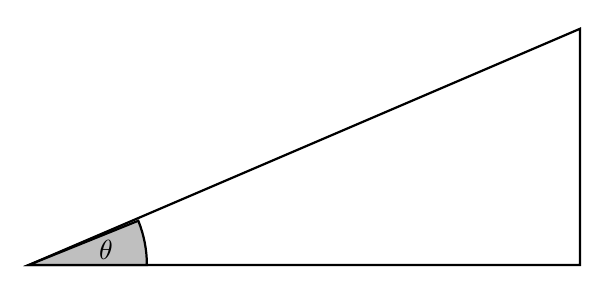
\begin{tikzpicture}[thick]
\coordinate (O) at (0,0);
\coordinate (A) at (7,0);
\coordinate (B) at (7,3);
\draw (O)--(A)--(B)--cycle;

%\tkzLabelSegment[below=2pt](O,A){\textit{adjacent leg}}
%\tkzLabelSegment[left=2pt](O,B){\textit{hypotenuse}}
%\tkzLabelSegment[above right=2pt](A,B){\textit{opposite leg}}

\tkzLabelSegment[below=5pt](O,A){\textit{x}}
\tkzLabelSegment[above left=5pt](O,B){\textit{r}}
\tkzLabelSegment[right=5pt](A,B){\textit{y}}

%\tkzMarkAngle[fill= orange,size=1.5cm, opacity=.4](A,O,B)
%\tkzLabelAngle[pos = 2](A,O,B){\texttt{$\theta$}}
 %%% AAAARGH ovan slutade funka så gjorde nedan HACK i stället
 \draw[fill=lightgray, thick] (0,0) -- (0:1.5cm) arc (0:22:1.5cm) node at (11:1.0cm) {$\theta$} -- cycle;

% \tkzMarkAngle[fill= orange,size=0.65cm, opacity=.4](A,O,B)
% \tkzLabelAngle[pos = 0.35](A,O,B){$\gamma$}
%
% \tkzMarkAngle[fill= orange,size=0.8cm, opacity=.4](B,A,O)
% \tkzLabelAngle[pos = 0.6](B,A,O){$\alpha$}
%
% \tkzMarkAngle[fill= orange,size=0.7cm, opacity=.4](O,B,A)
% \tkzLabelAngle[pos = 0.5](O,B,A){$\beta$}

\end{tikzpicture}

\item Du har nytta av metoderna \code{math.cos(theta)} och \code{math.sin(theta)} vid omvandling från polära koordinater.

\item Notera att klassens attribut är av typen \code{Double} och inte \code{Int}, trots att vi senare ska använda punkten för att beskriva en diskret pixelposition i ett \code{PixelWindow}. Anledningen till detta är att det kan uppstå avrundningsfel vid numeriska beräkningar. Detta blir särskilt märkbart vid upprepad räkning med små värden, t.ex. när man ritar en approximerad cirkel med många linjesegment.
\end{itemize}

\Subtask Klassen \code{PolygonWindow} nedan innehåller ett \code{PixelWindow} och ger möjlighet att rita ut polygoner. 
Kopiera koden för \code{PolygonWindow} till en ny kodfil \code{PolygonWindow.scala} i samma katalog som du placerade \code{Point} ovan i.

\begin{Code}
//> using dep "se.lth.cs::introprog:1.4.0"
package graphics

import introprog.PixelWindow
import java.awt.Color

extension def toPixels(p: Point): Seq[Int] = 
  Seq(point.x.round.toInt, point.y.round.toInt)

class PolygonWindow:
  val black     = Color(0,0,0)
  val coolGreen = Color(0,255,111)
  val width     = 500
  val height    = 500

  val window = 
    PixelWindow(width, height,  title = "Polygons", 
                background = black, foreground = coolGreen)

  def draw(polygon: Polygon): Unit =
    for i <- 0 until polygon.nbrOfCorners do
      val from = polygon.points(i).toPixels.map(_ + width / 2)
      val mod = polygon.points((i+1) % polygon.nbrOfCorners)
      val to = mod.toPixels.map(_ + width / 2)
      window.line(from(0), from(1), to(0), to(1), lineWidth = 2)
\end{Code}

Skapa en case-klass vid namn \code{Polygon} men en parameter \code{points: Vector[Point]} och ett attribut \code{val nbrOfCorners: Int}. Case-klassen \code{Polygon} ska också ligga i paketet \code{graphics}. 

Likt klassen \code{Point} ovan ska också \code{Polygon} ha ett kompanjonsobjekt. 
Kompanjonsobjektet ska ha en metod som skapar en regelbunden polygon vid namn \code{regular} med följande parametrar: \code{nbrOfCorners: Int, radius: Double, midPoint: Point}\\
Fundera över hur case-klassen \code{Polygon} och dess kompanjonsobjekt ska se ut för att koden ovan i \code{PolygonWindow} ska fungera som tänkt. Testa att allt fungerar i REPL.

\Subtask Kan man använda metoden \code{regularPolygon} för att rita cirklar? Kan man använda \code{Polygon} för att representera oregelbundna polygoner?
Testa i REPL.

\SOLUTION

\TaskSolved \what~

\Subtask \begin{Code}
package graphics

case class Point(x: Double, y: Double):
  val r: Double = math.hypot(x, y)
  val theta: Double = math.atan2(y, x)
  def +(p: Point): Point = Point(x + p.x, y + p.y)

object Point:
  def polar(r: Double, theta: Double): Point =
    Point(r * math.cos(theta), r * math.sin(theta))
\end{Code}

\Subtask \begin{Code}
package graphics

case class Polygon(points: Vector[Point]):
  val nbrOfCorners: Int = points.length
  
object Polygon:
  def regular(nbrOfCorners: Int, radius: Double, midPoint: Point): Polygon =
    val points = new Array[Point](nbrOfCorners)
    for i <- 0 until nbrOfCorners do
      val theta = i * (2 * math.Pi) / nbrOfCorners
      points(i) = Point.polar(radius, theta) + midPoint
    end for
    Polygon(points.toVector)
\end{Code}

\Subtask 
En perfekt cirkel går inte att skapa, men det går att komma tillräckligt nära för att göra det omöjligt att se hörnen.
Testa till exempel med 50 hörn likt nedan.
\begin{REPL}
scala> import graphics.*
scala> val circle = Polygon.regular(50,70,Point(-25,-25))
scala> val window = PolygonWindow()
scala> window.draw(circle)
\end{REPL}

Även en oregelbunden polygon går att skapa. Använd då konstruktorn till \code{Polygon} direkt. Till exempel likt nedan.
\begin{REPL}
scala> val irregular = 
         Polygon(Vector(Point(34,83), Point(16,42), Point(77,77), Point(100,138)))
scala> window.draw(irregular)
\end{REPL}

\QUESTEND




\WHAT{Klasser, instanser och skräp.}

\QUESTBEGIN

\Task  \what~För länge sedan i en galax långt långt borta...

\begin{Code}
case class Arm(ärTillVänster: Boolean)

case class Ben(ärTillVänster: Boolean)

case class Huvud(harHår: Boolean = true)

case class Rymdvarelse(
      arm1:   Arm   = Arm(true),
      arm2:   Arm   = Arm(false),
      ben1:   Ben   = Ben(true),
      ben2:   Ben   = Ben(false),
      huvud1: Huvud = Huvud(harHår = false),
  var huvud2: Huvud = Huvud()
):
  def ärSkallig = !huvud1.harHår && !huvud2.harHår
\end{Code}

\Subtask Klistra in ovan rymdkod i REPL och evaluera nedan rader. Rita minnessituationen efter rad 5 och beskriv vad som händer.
\begin{REPL}
scala> val alien = Rymdvarelse()
scala> alien.ärSkallig
scala> val predator = Rymdvarelse()
scala> predator.ärSkallig
scala> predator.huvud2 = alien.huvud1
scala> predator.huvud2 eq alien.huvud1  // test av referenslikhet
scala> println(predator)
scala> predator.ärSkallig
\end{REPL}

\Subtask Vad händer så småningom med det ursprungliga \code{huvud2}-objektet i predator efter tilldelningen på rad 5? Går det att referera till detta objekt på något sätt?

\SOLUTION

\TaskSolved \what

\SubtaskSolved  Vi skapar två rymdvarelser, \code{alien} och \code{predator}, med vardera två ben och två armar, samt vardera två huvuden (där det ena är skalligt och det andra har hår). Efter det är varken \code{alien} eller \code{predator} skallig eftersom båda har ett huvud med hår. Sen låter man referensen till \code{predator}s huvud med hår referera till aliens huvud utan hår. Nu är predator helt skallig och delar huvud med alien.

\includegraphics[scale=0.65]{../img/w06-solutions/2b}

\SubtaskSolved  Eftersom det inte längre finns någon referens som pekar på det objektet kommer skräpsamlaren att ta hand om det och det kommer förr eller senare skrivas över av något annat när platsen i minnet behövs. Objekt som inte har någon referens till sig går inte att komma åt.

\QUESTEND




\WHAT{Case-klass. Oföränderlig kvadrat.}

\QUESTBEGIN

\Task \label{task:Square} \what~

\Subtask Implementera nedan kvadrat med en editor och klistra in den i REPL.

\begin{Code}
case class Square(val x: Int = 0, val y: Int = 0, val side: Int = 1):
  val area: Int = ???

  /** Creates a new Square moved to position (x + dx, y + dy) */
  def moved(dx: Int, dy: Int): Square = ???

  def isEqualSizeAs(that: Square): Boolean = ???

  /** Multiplies the side with factor and rounded to nearest integer */
  def scale(factor: Double): Square = ???

object Square:
  /** A Square at (0, 0) with side 1 */
  val unit: Square = ???
\end{Code}

\Subtask Testa din kvadrat enligt nedan. Förklara vad som händer.

\begin{REPL}
scala> val (s1, s2) = (Square(), Square(1, 10, 1))
scala> val s3 = s1 moved (1,-5)
scala> s1 isEqualSizeAs s3
scala> s2 isEqualSizeAs s1
scala> s1 isEqualSizeAs Square.unit
scala> s2.scale(math.Pi) isEqualSizeAs s2
scala> s2.scale(math.Pi) isEqualSizeAs s2.scale(math.Pi)
scala> s2.scale(math.Pi) eq s2.scale(math.Pi)
scala> Square.unit eq Square.unit
\end{REPL}

\SOLUTION

\TaskSolved \what

\SubtaskSolved

\begin{Code}
case class Square(val x: Int = 0, val y: Int = 0, val side: Int = 1):
  val area: Int = side * side

  def moved(dx: Int, dy: Int): Square = Square(x + dx, y + dy, side)

  def isEqualSizeAs(that: Square): Boolean = this.side == that.side

  def scale(factor: Double): Square =
    Square(x, y, (side * factor).round.toInt)

object Square:
  val unit: Square = Square()
\end{Code}

\SubtaskSolved
\begin{REPL}
scala> val (s1, s2) = (Square(), Square(1, 10, 1))
val s1: Square = Square(0,0,1)
val s2: Square = Square(1,10,1)

scala> val s3 = s1 moved (1,-5)
val s3: Square = Square(1,-5,1)

scala> s1 isEqualSizeAs s3       // lika storlek
val res0: Boolean = true

scala> s2 isEqualSizeAs s1       // lika storlek
val res1: Boolean = true

scala> s1 isEqualSizeAs Square.unit   // s1 har sidan 1
val res2: Boolean = true

scala> s2.scale(math.Pi) isEqualSizeAs s2  // olika storlek
val res3: Boolean = false

scala> s2.scale(math.Pi) == s2.scale(math.Pi) // lika innehåll
val res4: Boolean = true

scala> s2.scale(math.Pi) eq s2.scale(math.Pi)  // olika objekt
val res5: Boolean = false

scala> Square.unit eq Square.unit   // samma objekt
val res6: Boolean = true
\end{REPL}

\QUESTEND




\clearpage

\AdvancedTasks %%%%%%%%%%%%%%%%%%%%%%%%%%%%%%%%%%%%%%%%%%%%%%%%%%%%%%%%%%%%%%%%%

\WHAT{Innehållslikhet mellan olika typer.}

\QUESTBEGIN

\Task \what~Klistra in nedan klasser i REPL och undersök vad som händer.

\begin{Code}
class Gurka(val vikt: Int)

class Bil(val typ: String)
\end{Code}

\begin{REPL}
scala> class Gurka(val vikt: Int)
     |
     | class Bil(val typ: String)
// defined class Gurka
// defined class Bil

scala> 42 == "Fyrtiotvå"

scala> Gurka(50) == Bil("Sedan")

\end{REPL}

Finns det något resultat som är problematiskt, och i så fall, varför?


\SOLUTION

\TaskSolved \what~
\begin{REPL}
scala> 42 == "Fyrtiotvå"
1 |42 == "Fyrtiotvå"
  |^^^^^^^^^^^^^^^^^
  |Values of types Int and String cannot be compared with == or !=

scala> Gurka(50) == Bil("Sedan")
val res0: Boolean = false
\end{REPL}

Det andra uttrycket är problematiskt eftersom det alltid kommer resultera i \code|false|, då klasserna \code|Gurka| och \code|Bil| är två ojämförbara typer som inte bör jämföras med avseende på innehållslikhet. Detta försämrar typsäkerheten vilket ökar risken för svårupptäckta buggar där fel typer jämförs.

Likhetsjämförelser som sker mellan primitiva typer typkollas av kompilatorn och kan därför ge kompileringsfel om två olika typer, såsom \code|Int| och \code|String|, jämförs med varandra. Detta gäller dock i regel inte egendefinierade typer, vilket alltså innebär att en likhetsjämförelse mellan olika egendefinierade typer alltid resulterar i \code|false|.

Det är emellertid möjligt att få samma typkoll för egendefinierade typer som för primitiva typer genom att importera \code|scala.language.strictEquality|.

\begin{Code}
import scala.language.strictEquality
class Gurka(val vikt: Int)

class Bil(val typ: String)
\end{Code}

\begin{REPL}
scala> Gurka(50) == Bil("Sedan")
1 |Gurka(50) == Bil("Sedan")
  |^^^^^^^^^^^^^^^^^^^^^^^^^
  |Values of types Gurka and Bil cannot be compared with == or !=
\end{REPL}

\QUESTEND


\WHAT{Attributrepresentation. Privat konstruktor. Fabriksmetod.}

\QUESTBEGIN

\Task \what~Kim Kodkunnig skapade för länge sedan denna klass som används på många ställen i befintlig kod:

\begin{Code}
class Point private (val x: Int, val y: Int)
object Point:
  def apply(x: Int = 0, y: Int = 0): Point = new Point(x, y)
  val origo = apply()
\end{Code}

\Subtask Vad händer om du försöker instansiera Kim Kodkunnigs klass direkt med nyckelordet \code{new}?

\Subtask Varför använder Kim Kodkunnig ett kompanjonsobjekt med en fabriksmetod? Vilka accessregler gäller mellan ett kompanjonsobjekt och klassen med samma namn?

\Subtask Hjälp Kim Kodkunnig att ändra attributrepresentationen så att det oföränderliga tillståndet utgörs av en 2-tupel \code{val p: (Int, Int)} i stället. Befintlig kod ska inte behöva ändras och klassen \code{Point} ska bete sig från ''utsidan'' precis som innan.

\SOLUTION

\TaskSolved \what~

\SubtaskSolved Det blir kompileringsfel eftersom konstruktorn är privat.
\begin{REPL}
scala> class Point private (val x: Int, val y: Int)
     | object Point:
     |   def apply(x: Int = 0, y: Int = 0): Point = new Point(x, y)
     |   val origo = apply()
     |
// defined class Point
// defined object Point

scala> new Point(0, 0)
1 |new Point(0, 0)
  |    ^^^^^
  |constructor Point cannot be accessed as a member of Point from module class
\end{REPL}

\SubtaskSolved
\begin{itemize}
  \item Genom att ha en privat konstruktor och bara göra indirekt instansiering via fabriksmetod är lätt ändra attributrepresentation i framtiden utan att befintlig kod behöver ändras.

  \item Accessreglerna för kompanjonsobjekt är sådana att kompanjoner ser varandras privata delar.
\end{itemize}

\SubtaskSolved

\begin{Code}
class Point private (private val p: (Int, Int)):
  def x: Int = p._1
  def y: Int = p._2

object Point:
  def apply(x: Int = 0, y: Int = 0): Point = new Point(x, y)
  val origo = apply()
\end{Code}

\QUESTEND



\WHAT{Synlighet av klassparametrar och konstruktor, \code{private[this]}.}

\QUESTBEGIN

\Task  \what~

\Subtask En av gurk-klasserna nedan är trasig. Varför och vad blir det för fel?

\begin{Code}
class Gurka1(vikt: Int)

class Gurka2(val vikt: Int)

class Gurka3(private val vikt: Int)

class Gurka4(private val vikt: Int, kompis: Gurka4):
  def kompisVikt = kompis.vikt

class Gurka5(private[this] val vikt: Int, kompis: Gurka5):
  def kompisVikt = kompis.vikt

class Gurka6 private (vikt: Int)

class Gurka7 private (var vikt: Int)
object Gurka7:
  def apply(vikt: Int) =
    require(vikt >= 0, "negativ vikt: " + vikt)
    new Gurka7(vikt)
\end{Code}

\Subtask Undersök nedan vad nyckelorden \code{val} och \code{private} får för konsekvenser. Förklara vad som händer. Vilka rader ger vilka felmeddelanden?

\begin{REPL}
scala> new Gurka1(42).vikt
scala> new Gurka2(42).vikt
scala> new Gurka3(42).vikt
scala> val ingenGurka: Gurka4 = null
scala> new Gurka4(42, ingenGurka).kompisVikt
scala> new Gurka4(42, new Gurka4(84, null)).kompisVikt
scala> new Gurka6(42)
scala> new Gurka7(-42)
scala> Gurka7(-42)
scala> val g = Gurka7(42)
scala> g.vikt
scala> g.vikt = -1
scala> g.vikt
\end{REPL}


\SOLUTION


\TaskSolved \what

\SubtaskSolved \code{Gurka5} är trasig. Eftersom vikten i \code{Gurka5} är privat för instansen och inte klassen, kan en instans inte accessa en annan instans vikt.
\begin{REPL}
11 |  def kompisVikt = kompis.vikt
   |                   ^^^^^^^^^^^
   |value vikt cannot be accessed as a member of (Gurka5.this.kompis : Gurka5) from class Gurka5.
\end{REPL}


\SubtaskSolved
\begin{REPL}
scala> new Gurka1(42).vikt
1 |new Gurka1(42).vikt
  |^^^^^^^^^^^^^^^^^^^
  |value vikt cannot be accessed as a member of Gurka1 from module class

scala> new Gurka2(42).vikt
val res0: Int = 42

scala> new Gurka3(42).vikt
1 |new Gurka3(42).vikt
  |^^^^^^^^^^^^^^^^^^^
  |value vikt cannot be accessed as a member of Gurka3 from module class

scala> val ingenGurka: Gurka4 = null
val ingenGurka: Gurka4 = null

scala> new Gurka4(42, ingenGurka).kompisVikt
java.lang.NullPointerException: Cannot invoke "rs$line$1$Gurka4.vikt()" bec...
  at rs$line$1$Gurka4.kompisVikt(rs$line$1:8)
  ... 38 elided

scala> new Gurka4(42, new Gurka4(84, null)).kompisVikt
val res2: Int = 84

scala> new Gurka6(42)
1 |new Gurka6(42)
  |    ^^^^^^
  |constructor Gurka6 cannot be accessed as a member of Gurka6 from module...

scala> new Gurka7(-42)
1 |new Gurka7(-42)
  |    ^^^^^^
  |constructor Gurka7 cannot be accessed as a member of Gurka7 from module...

scala> Gurka7(-42)
java.lang.IllegalArgumentException: requirement failed: negativ vikt: -42

scala> val g = Gurka7(42)
val g: Gurka7 = Gurka7@51fd1c7c

scala> g.vikt
val res4: Int = 42

scala> g.vikt = -1

scala> g.vikt
val res5: Int = -1
\end{REPL}

\QUESTEND





\WHAT{Egendefinierad setter kombinerat med privat konstruktor.}

\QUESTBEGIN

\Task  \what~Klistra in denna kod i REPL:

\begin{Code}
class Gurka8 private (private var _vikt: Int):
  def vikt = _vikt
  def vikt_=(v: Int): Unit =
    require(v >= 0, "negativ vikt: " +v)
    _vikt = v

object Gurka8:
  def apply(vikt: Int) =
    require(vikt >= 0, "negativ vikt: " + vikt)
    new Gurka8(vikt)
\end{Code}


\Subtask Förklara vad som händer nedan. Vilka rader ger vilka felmeddelanden?
\begin{REPL}
scala> val g = Gurka8(-42)
scala> val g = Gurka8(42)
scala> g.vikt
scala> g.vikt = 0
scala> g.vikt = -1
scala> g.vikt += 42
scala> g.vikt -= 1000
\end{REPL}

\Subtask Vad är fördelen med möjligheten att skapa egendefinierade setters?

\SOLUTION


\TaskSolved \what


\SubtaskSolved

Rad 1:
\begin{REPL}
	java.lang.IllegalArgumentException: requirement failed: negativ vikt: -42
\end{REPL}
\code{Gurka8.apply} kräver att \code{vikt >= 0} annars kastar \code{require} ett undantag.

Rad 5:
\begin{REPL}
	java.lang.IllegalArgumentException: requirement failed: negativ vikt: -1
\end{REPL}
Settern \code{vikt_=} kräver att \code{vikt >= 0} annars kastar \code{require} ett undantag.

Rad 7:
\begin{REPL}
	java.lang.IllegalArgumentException: requirement failed: negativ vikt: -958
\end{REPL}
Eftersom \code{42 - 1000} är mindre än noll kastar \code{require} ett undantag.

\SubtaskSolved  Man kan sätta egna mer specifika krav på vad som får göras med värdena så man har större koll på att inget oväntat händer.

\QUESTEND




\WHAT{Objekt med föränderligt tillstånd \Eng{mutable state}.}

\QUESTBEGIN

\Task  \what~  Du ska implementera en modell av en hoppande groda som uppfyller följande krav:
\begin{enumerate}%[nolistsep, noitemsep]
\item Varje grodobjekt ska hålla reda på var den är.
\item Varje grodobjekt ska hålla reda på hur långt grodan hoppat totalt.
\item Varje grodobjekt ska kunna beräkna hur långt det är mellan grodans nuvarande position och utgångsläget.
\item Alla grodor börjar sitt hoppande i origo.
\item En groda kan hoppa enligt två metoder:
  \begin{itemize} [nolistsep, noitemsep]
  \item relativ förflyttning enligt parametrarna \code{dx} och \code{dy},
  \item slumpmässig relativ förflyttning $[1, 10]$ i x-ledsförändring och $[1, 10]$ i y-ledsförändring.
  \end{itemize}
\end{enumerate}

\Subtask Implementera klassen \code{Frog} enligt nedan kodskelett och ovan krav.

\begin{Code}
class Frog private (initX: Int = 0, initY: Int = 0):
  def x: Int = ???
  def y: Int = ???

  def jump(dx: Int, dy: Int): Unit = ???
  def randomJump: Unit = ???

  def distanceToStart: Double = ???
  def distanceJumped: Double = ???
  def distanceTo(that: Frog): Double = ???

object Frog:
  def spawn(): Frog = ???
\end{Code}
\emph{Tips:}
\begin{itemize} [nolistsep, noitemsep]
\item Om namnet man vill ge ett privat föränderligt attribut ''krockar'' med ett metodnamn, är det vanligt att man börjar attributets namn med understreck, t.ex. \code{private var _x } för att på så sätt undkomma namnkonflikten.
\item Inför en metod i taget och klistra in den nya grodan i REPL efter varje utvidgning och testa.
\end{itemize}



\Subtask Skapa en metod \code{def test(): Unit} i ett singelobjekt \code{FrogTest} som innehåller kod som gör minst en kontroll av varje krav. Om ingen kontroll går fel ska \code{"Test Ok!"} skrivas ut, annars ska exekveringen avbrytas. \emph{Tips:} Använd \code{assert(b, msg)} som avbryter exekveringen och skriver ut \code{msg} om \code{b} är falsk.

\Subtask Vad kallas en metod som enbart returnerar värdet av ett privat attribut?

\Subtask Inför setters för attributen som håller reda på x- och y-postitionen. Förändringar av positionen i x- eller y-led ska räknas som ett hopp och alltså registreras i det attribut som håller reda på det ackumulerade hoppavståndet.

\Subtask Simulera ett massivt grodhoppande med krockdetektering genom att skapa 100 grodor som till att börja med är placerade på x-axeln med avståndet $8$ längdenheter mellan sig. För varje runda i en \code{while}-sats, låt en slumpässigt vald groda göra ett \code{randomJump} tills någon groda befinner sig närmare än $0.5$ längdenheter, vilket är definitionen på att de har krockat. Räkna hur många looprundor som behövs innan något grodpar krockar och skriv ut antalet. Skriv även ut det totala antalet \\ \emph{Tips:} Börja med pseudokod på papper. Använd en grodvektor.


\SOLUTION


\TaskSolved \what


\SubtaskSolved
\begin{Code}
class Frog private (initX: Int = 0, initY: Int = 0):
  private var _x: Int = initX
  private var _y: Int = initY
  private var _distanceJumped: Double = 0

  def x: Int = _x
  def y: Int = _y

  def jump(dx: Int, dy: Int): Unit =
    _x += dx
    _y += dy
    _distanceJumped += math.hypot(dx, dy)


  def randomJump: Unit =
    def rnd = util.Random.nextInt(10) + 1
    jump(rnd, rnd)

  def distanceToStart: Double = math.hypot(x,y)
  def distanceJumped: Double = _distanceJumped
  def distanceTo(f: Frog): Double = math.hypot(x - f.x, y - f.y)

object Frog:
  def spawn(): Frog = Frog()
\end{Code}

\SubtaskSolved Exempel på testprogram:
\begin{Code}
object FrogTest:
  def test(): Unit =
    val f1 = Frog.spawn()
    assert(f1.x == 0 && f1.y == 0, "Test of spawn, reqt 1 & 4 failed.")

    f1.jump(4, 3)
    assert(f1.x == 4 && f1.y == 3, "Test of jump, reqt 1 & 4 failed.")

    f1.jump(4, 3)
    assert(f1.distanceJumped == 10, "Test of jump, reqt 2 failed.")

    f1.jump(-4, -3)
    assert(f1.distanceToStart == 5, "Test of jump, reqt 3 failed.")

    for x <- 1 to 10000 do
      val f2 = Frog.spawn()
      f2.randomJump
      assert(f2.x > 0 && f2.x <= 10 && f2.y > 0 && f2.y <= 10,
        "Test of randomJump, reqt 5 failed.")

    println("Test Ok!")
\end{Code}

\SubtaskSolved  En metod som är en indirekt avläsning av attributvärden kallas getter.

\SubtaskSolved
\begin{Code}
class Frog private (initX: Int = 0, initY: Int = 0):
  private var _x: Int = initX
  private var _y: Int = initY
  private var _distanceJumped: Double = 0

  def jump(dx: Int, dy: Int): Unit =
    _x += dx
    _y += dy
    _distanceJumped += math.hypot(dx, dy)

  def x: Int = _x
  def x_=(newX: Int): Unit = // Setter för x
    _distanceJumped += math.abs(x - newX)
    _x = newX

  def y: Int = _y
  def y_=(newY: Int): Unit = // Setter för y
    _distanceJumped += math.abs(y - newY)
    _y = newY


  def randomJump: Unit =
    def rnd = util.Random.nextInt(10) + 1
    jump(rnd, rnd)

  def distanceToStart: Double = math.hypot(x,y)
  def distanceJumped: Double = _distanceJumped
  def distanceTo(f: Frog): Double = math.hypot(x - f.x, y - f.y)

object Frog:
  def spawn(): Frog = Frog()
\end{Code}

\SubtaskSolved
\begin{Code}
object FrogSimulation:
  def isAnyCollision(frogs: Vector[Frog]): Boolean =
    var found = false
    frogs.indices.foreach(i =>  // generate all pairs (i,j)
      for j <- i + 1 until frogs.size do
        if !found then
          found = frogs(i).distanceTo(frogs(j)) <= 0.5
    )
    found

  def jumpUntilCrash(n: Int = 100, initDist: Int = 8): (Int, Double) =
    val frogs = Vector.fill(n)(Frog.spawn())
    (0 until n).foreach(i => frogs(i).x = i * initDist)
    var count = 0
    while !isAnyCollision(frogs) do
      frogs(util.Random.nextInt(n)).randomJump
      count += 1
    (count, frogs.map(_.distanceJumped).sum)


  def run(nbrOfCrashTests: Int = 10) =
    for i <- 1 to nbrOfCrashTests do
      val (n, dist) = jumpUntilCrash()
      println(s"\nAntalet looprundor innan grodkrock: $n")
      println(s"Totalt avstånd hoppat av alla grodor: $dist")
\end{Code}

\QUESTEND




\QUESTBEGIN

\Task  \what~  Webbshoppen \textbf{UberSquare} säljer flyttbara kvadrater. I affärsmodellen ingår att ta betalt per förflyttning. Du ska hjälpa UberSquare att utveckla en enkel prototyp för att imponera på riskkapitalister. (En variant av denna uppgift ingick i tentamen 2017-08-23.)

\Subtask Implementera \code{Square} enligt dokumentationskommentarerna i efterföljande kodskiss och enligt dessa krav:

\begin{enumerate}%[nolistsep, noitemsep]
   \item Varje instans av \code{Square} ska räkna antalet förflyttningar som gjorts sedan instansen konstruerats.

   \item För att kunna övervaka sina kunder vill UberSquare även räkna det totala antalet förflyttningar som gjorts av alla kvadrater som någonsin skapats (s.k. \emph{big data}).

  \item Varje gång förflyttning sker ska ett visst belopp adderas till den ackumulerade kostnaden för respektive kvadrat, enligt kostnadsberäkningen i krav 4.

  \item UberSquare är oroliga för att kvadraterna flyttas för långt bort och bestämmer därför att för varje förflyttning ska den ackumulerade kvadratkostnaden ökas med den nya positionens avstånd till ursprungsläget vid kvadratens konstruktion multiplicerat med aktuell storlek på kvadraten.

  \item För att framstå som goda berättar UberSquare i sin marknadsföring att det är gratis att skala kvadrater. \footnote{D.v.s. ett anrop av metoden \code{scale} orsakar ingen omedelbar kostnad.}
\end{enumerate}

\begin{CodeSmall}
/** A mutable and expensive Square. */
class Square private (val initX: Int, val initY: Int, val initSide: Int):
  private var nMoves = 0
  private var sumCost = 0.0

  private var _x = initX
  private var _y = initY

  private var _side = initSide

  private def addCost(): Unit =
    sumCost += ???

  def x: Int = ???
  def y: Int = ???

  def side = ???

  /** Scales the side of this square and rounds it to nearest integer */
  def scale(factor: Double): Unit = ???

  /** Moves this square to position (x + xd, y + dy) */
  def move(dx: Int, dy: Int): Unit = ???

  /** Moves this square to position (x, y) */
  def moveTo(x: Int, y: Int): Unit = ???

  /** The accumulated cost of this Square */
  def cost: Double = ???

  /** Returns the accumulated cost. Sets the accumulated cost to zero. */
  def pay: Double = ???

  override def toString: String =
    s"Square[($x, $y), side: $side, #moves: $nMoves times, cost: $sumCost]"


object Square:
  private var created = Vector[Square]()

  /** Constructs a new Square object at (x, y) with size side */
  def apply(x: Int, y: Int, side: Int): Square =
    require(side >= 0, s"side must be positive: $side")
    ???

  /** Constructs a new Square object at (0, 0) with side 1 */
  def apply(): Square = ???

  /** The total number of moves that have been made for all squares. */
  def totalNumberOfMoves: Int = ???

  /** The total cost of all squares. */
  def totalCost: Double = ???
\end{CodeSmall}

\Subtask Testa din kvadratprototyp i REPL. Använd t.ex. koden nedan:
\begin{REPL}
scala> val xs = Vector.fill(10)(Square())
scala> xs.foreach(_.move(2, 3))
scala> xs.foreach(_.scale(2.9))
scala> val (m, c) = (Square.totalNumberOfMoves, Square.totalCost)
val m: Int = 10
val c: Double = 36.055512754639885
\end{REPL}

\SOLUTION

\TaskSolved \what~

\begin{CodeSmall}
class Square private (val initX: Int, val initY: Int, val initSide: Int):
  private var nMoves = 0
  private var sumCost = 0.0

  private var _x = initX
  private var _y = initY

  private var _side = initSide

  private def addCost(): Unit =
    sumCost += math.hypot(x - initX, y - initY) * side

  def x: Int = _x
  def y: Int = _y

  def side = _side

  def scale(factor: Double): Unit = _side = (_side * factor).round.toInt

  def move(dx: Int, dy: Int): Unit =
    _x += dx; _y += dy
    nMoves += 1
    addCost()

  def moveTo(x: Int, y: Int): Unit =
    _x = x; _y = y
    nMoves += 1
    addCost()

  def cost: Double = sumCost

  def pay: Double = {val temp = sumCost; sumCost = 0; temp}

  override def toString: String =
    s"Square[($x, $y), side: $side, #moves: $nMoves times, cost: $sumCost]"

object Square:
  private var created = Vector[Square]()

  def apply(x: Int, y: Int, side: Int): Square =
    require(side >= 0, s"side must be positive: $side")
    val sq = (new Square(x, y, side))
    created :+= sq
    sq

  def apply(): Square = apply(0, 0, 1)

  def totalNumberOfMoves: Int = created.map(_.nMoves).sum

  def totalCost: Double = created.map(_.cost).sum
\end{CodeSmall}

\QUESTEND



\WHAT{Hjälpkonstruktor.}

\QUESTBEGIN

\Task\Uberkurs \label{task:aux-constructor} \what~I tidigare uppgifter har vi möjliggjort alternativa sätt att skapa instanser genom default-argument och fabriksmetoder i kompanjonsobjekt.

Ett annat sätt att göras detta på, som i Scala är ovanligt\footnote{Men i Java är detta mycket vanligt då defaultargument m.m. inte ingår i språket.}, är att definiera flera konstruktorer inne i klasskroppen. I Scala kallas en sådan extra konstruktor för \textbf{hjälpkonstruktor} \Eng{auxiliary constructor}.

En hjälpkonstruktor skapar man i Scala genom att definiera en metod som har det speciella namnet \code{this}, alltså en deklaration \code{def this(...) = ...} Hjälpkonstruktorer måste börja med att anropa en annan konstruktor, antingen den primära konstruktorn (d.v.s. den som klasshuvudet definierar) eller en tidigare definierad  hjälpkonstruktor.

\Subtask Läs mer om hjälpkonstruktorer här: \\ \href{http://www.artima.com/pins1ed/functional-objects.html#6.7}{www.artima.com/pins1ed/functional-objects.html\#6.7}

\Subtask Hitta på en egen uppgift med hjälpkonstruktorer, baserat på någon av klasserna i tidigare övningar.


%\Task \TODO \\ \code{class Rational private (numerator: BigInt, denominator: BigInt)} \\
%Inspirerat av Rational i pins1ed med GCD\SOLUTION

\QUESTEND


%!TEX encoding = UTF-8 Unicode
%!TEX root = ../exercises.tex

\ifPreSolution



\Exercise{\ExeWeekSIX}\label{exe:W06}

\begin{Goals}
\item Kunna skapa och använda \code{match}-uttryck med konstanta värden, garder och mönstermatchning med case-klasser.
\item Kunna skapa och använda case-objekt för matchningar på uppräknade värden.
\item Kunna hantera saknade värden med hjälp av typen \code{Option} och mönstermatchning på \code{Some} och \code{None}.
\item Kunna fånga undantag med \code{scala.util.Try}.
\item Känna till \code{try}, \code{catch} och \code{throw}.
%\item Känna till \jcode{switch}-satser i Java.
\item Känna till nyckelordet \code{sealed} och förstå nyttan med förseglade typer.
%\item Känna till relationen mellan \code{hashCode} och \code{equals}.
%\item Kunna skapa partiella funktioner med case-uttryck.
%\item Känna till betydelsen av små och stora begynnelsebokstäver i case-grenar i en matchning, samt förstå hur namn binds till värden in en case-gren.
%\item Kunna använda \code{flatMap} tillsammans med \code{Option} och \code{Try}.
%\item Känna till skillnaderna mellan \code{try}-\code{catch} i Scala och java.
%\item Känna till att metoden \code{unapply} används vid mönstermatchning.
%\item Kunna implementera \code{equals} med hjälp av en \code{match}-sats, som fungerar för finala klasser utan arv.
%\item Känna till \code{null}.
\end{Goals}

\begin{Preparations}
\item \StudyTheory{06}
\end{Preparations}

\BasicTasks %%%%%%%%%%%%%%%%

\else



\ExerciseSolution{\ExeWeekSIX}

\BasicTasks %%%%%%%%%%%

\fi




\WHAT{Matcha på konstanta värden.}

\QUESTBEGIN

\Task \label{task:vegomatch} \what~   % I Scala finns ingen \jcode{switch}-sats. I stället har Scala ett \code{match}-uttryck som är mer kraftfullt. Dock saknar Scala nyckelordet \jcode{break} och Scalas \code{match}-uttryck kan inte ''falla igenom'' som skedde i uppgift \ref{task:switch}\ref{subtask:break}.

\Subtask \label{subtask:vegomatch} Skriv nedan program med en kodeditor och spara i filen \texttt{Match.scala}. Kompilera och kör och och ge som argument din favoritgrönsak. Vad händer? Förklara hur ett \code{match}-uttryck fungerar.

\scalainputlisting[numbers=left,basicstyle=\ttfamily\fontsize{11}{12}\selectfont]{examples/Match.scala}

\Subtask Vad blir det för felmeddelande om du tar bort case-grenen för defaultvärden och indata väljs så att inga case-grenar matchar? Är det ett exekveringsfel eller ett kompileringsfel?

% \Subtask Beskriv några skillnader i syntax och semantik mellan Javas flervalssats \jcode{switch} och Scalas flervalsuttryck \code{match}.



\SOLUTION


\TaskSolved \what


\SubtaskSolved  %Svaret blir identiskt mot föregående uppgiften i Java.\\
Scalas \code{match}-uttryck jämför stegvis värdet med varje \code{case} för att sedan returnera ett värde tillhörande motsvarande \code{case}.

\SubtaskSolved  \begin{REPL}
scala.MatchError 
\end{REPL}
Exekveringsfel, uppstår av en viss input under körningen.

% \SubtaskSolved  Scalas \code{match} ersätter kolonet (:) i \jcode{switch} med Scalas högerpil (=>).\\
% \code{match} returnerar ett värde till skillnad från \jcode{switch} som inte returnerar något.\\
% \code{match} kan inte $"$falla igenom$"$ så ett \jcode{break} efter varje \jcode{case} är inte nödvändigt.\\
% Till skillnad från \jcode{switch}-satsen kastar \code{match} ett \code{MatchError} om ingen matchning skulle ske.



\QUESTEND






\WHAT{Gard i case-grenar.}

\QUESTBEGIN

\Task  \what~  Med hjälp en gard \Eng{guard} i en case-gren kan man begränsa med ett villkor om grenen ska väljas.

Utgå från koden i uppgift \ref{task:vegomatch}\ref{subtask:vegomatch} och byt ut case-grenen för \code{'g'}-matchning till nedan variant med en gard med nyckelordet \code{if} (notera att det inte behövs parenteser runt villkoret):
\begin{Code}
    case 'g' if math.random() > 0.5 => "gurka är gott ibland..."
\end{Code}
Kompilera om och kör programmet upprepade gånger med olika indata tills alla grenar i \code{match}-uttrycket har exekverats. Förklara vad som händer.

\SOLUTION


\TaskSolved \what

Garden som införts vid \code{case 'g'} slumpar fram ett tal mellan 0 och 1 och om talet inte är större än $0.5$ så blir det ingen matchning med \code{case 'g'} och programmet testar vidare tills default-caset.\\
Gardens krav måste uppfyllas för att det ska matcha som vanligt.



\QUESTEND






\WHAT{Mönstermatcha på attributen i case-klasser.}

\QUESTBEGIN

%\Task \label{task:match-caseclass} \what~   Scalas \code{match}-uttryck är extra kraftfulla om de används tillsammans med \code{case}-klasser: då kan attribut extraheras automatiskt och bindas till lokala variabler direkt i case-grenen som nedan exempel visar (notera att \code{v} och \code{rutten} inte behöver deklareras explicit). Detta kallas för \textbf{mönstermatchning}.

\Task \label{task:match-caseclass} \what~   Scalas \code{match}-uttryck är extra kraftfulla om de används tillsammans med \code{case}-klasser: då kan attribut extraheras automatiskt och bindas till lokala variabler direkt i case-grenen som nedan exempel visar (notera att \code{v} och \code{rutten} inte behöver deklareras explicit). Detta kallas för \textbf{mönstermatchning}. 
Vad skrivs ut nedan? Varför? Prova att byta namn på \code{v} och \code{rutten}.
%\Subtask \label{subtask:autobinding-match} Vad skrivs ut nedan? Varför? Prova att byta namn på \code{v} och \code{rutten}.
\begin{REPL}
scala> case class Gurka(vikt: Int, ärRutten: Boolean)
scala> val g = Gurka(100, true)
scala> g match { case Gurka(v,rutten) => println("G" + v + rutten) }
\end{REPL}

%\TODO %Tab två gånger fungerar inte i scala3-repl, issue #536
%\Subtask Skriv sedan nedan i REPL och tryck TAB två gånger efter punkten. Vad har \code{unapply}-metoden för resultattyp?
%\begin{REPL}
%scala> Gurka.unapply   // Tryck TAB två gånger
%\end{REPL}
%\begin{Background}
%Case-klasser får av kompilatorn automatiskt ett kompanjonsobjekt \Eng{companion object}, i detta fallet \code{object Gurka}. Det objektet får av kompilatorn automatiskt en \code{unapply}-metod. Det är \code{unapply} som anropas ''under huven'' när case-klassernas attribut extraheras vid mönstermatchning, men detta sker alltså automatiskt och man behöver inte explicit nyttja \code{unapply} om man inte själv vill implementera s.k. extraherare \Eng{extractors}; om du är nyfiken på detta, se fördjupningsuppgift \ref{task:extractor}.
%\end{Background}

%\Subtask Anropa \code{unapply}-metoden enligt nedan. Vad blir resultatet?
%\begin{REPL}
%scala> Gurka.unapply(g)
%\end{REPL}
%Vi ska i senare uppgifter undersöka hur typerna \code{Option} och \code{Some} fungerar och hur man kan ha nytta av dessa i andra sammanhang.

% \Subtask Spara programmet nedan i filen \texttt{vegomatch.scala} och kompilera och kör med \code{scala vegomatch.Main 1000} i terminalen. Förklara hur predikatet \code{ärÄtvärd} fungerar.
% \scalainputlisting[numbers=left,basicstyle=\ttfamily\fontsize{11}{12}\selectfont]{examples/vegomatch.scala}
%

\SOLUTION


\TaskSolved \what \\
G100true. Vid byte av plats: Gtrue100.\\
\code{match} testar om kompanjonsobjektet \code{Gurka} är av typen \code{Gurka} med två parametervärden. De angivna parametrarna tilldelas namn, \code{vikt} får namnet \code{v} och \code{ärRutten} namnet \code{rutten} och skrivs sedan ut. Byts namnen dessa ges skrivs de ut i den omvända ordningen.

%\TODO % TAB+TAB fungerar inte i scala3-repl så svaret till uppgiften är felaktig
%\SubtaskSolved  \code{Option[(Int, Boolean)]}

%\SubtaskSolved	\code{Gurka(100, true)}

% \SubtaskSolved  \code{ärÄtvärd} testar om \code{Grönsak g} är av typen \code{Gurka(v, rutten)} eller \code{Tomat}. Dessa har sedan garder.\\ \code{Gurka} måste ha \code{vikt} över 100 och \code{ärRutten} vara \code{false} för att \code{case Gurka} ska returnera \code{true}.\\
% \code{Tomat} måste ha \code{vikt} över 50 och \code{ärRutten} vara \code{false} för att \code{case Tomat} ska returnera \code{true}.\\
% Matchas inte \code{Grönsak g} med någon av dessa returneras default-värdet \code{false}.



\QUESTEND







\WHAT{Matcha på case-objekt och nyttan med \code{sealed}.}

\QUESTBEGIN

\Task	\label{task:match-sealedtrait} \what~	Skriv nedan kodrader i en REPL en för en. Notera nyckelordet \code{sealed} som används för att försegla en typ. En \textbf{förseglad typ} måste ha alla sina subtyper i en och samma kodfil.
\begin{REPL}
scala> sealed trait Färg
scala> case object Spader extends Färg
\end{REPL}
\Subtask Hur lyder felmeddelandet och varför sker det? Är det ett kompileringsfel eller ett körtidsfel?

\Subtask  \label{subtask:match-sealedtrait-caseobject}
Skapa nu nedan kod i en editor och klistra in i REPL.
\begin{Code}
object Kortlek:
  sealed trait Färg
  object Färg:
      val values = Vector(Spader, Hjärter, Ruter, Klöver)
  case object Spader extends Färg
  case object Hjärter extends Färg
  case object Ruter extends Färg
  case object Klöver extends Färg
\end{Code}

\Subtask \label{subtask:match-sealedtrait-function}
Skapa en funktion \code{def parafärg(f: Färg): Färg} i en editor, som med hjälp av ett match-uttryck returnerar parallellfärgen till en färg. Parallellfärgen till \code{Hjärter} är \code{Ruter} och vice versa, medan parallellfärgen till \code{Klöver} är \code{Spader} och vice versa. Klistra in funktionen i REPL. Passa även på att skriva en \code{import}-sats för det yttre objektet \textbf{Kortlek}, så medlemmarna av objektet kan nås enkelt.
\begin{REPL}
scala> parafärg(Spader)
scala> val xs = Vector.fill(5)(Färg.values((math.random() * 4).toInt))
scala> xs.map(parafärg)
\end{REPL}

\Subtask \label{subtask:match-forgetcase}
Vi ska nu undersöka vad som händer om man glömmer en av case-grenarna i matchningen i \code{parafärg}. ''Glöm'' alltså avsiktligt en av case-grenarna och klistra in den nya \code{parafärg} med den ofullständiga matchningen. Hur lyder varningen? Kommer varningen vid körtid eller vid kompilering?

\Subtask Anropa \code{parafärg} med den ''glömda'' färgen. Hur lyder felmeddelandet? Är det ett kompileringsfel eller ett körtidsfel?

\Subtask Förklara vad nyckelordet \code{sealed} innebär och vilken nytta man kan ha av att \textbf{försegla} en supertyp.


\SOLUTION


\TaskSolved \what

\SubtaskSolved
\begin{REPL}
Cannot extend sealed trait Färg in a different source file
\end{REPL}
Felmeddelandet fås av att REPL:en behandlar varje inmatning individuellt och tillåter därför inte att subtypen \code{Spader} ärver från \Eng{extends} supertypen \code{Färg} eftersom denna var förseglad \Eng{sealed}. Mer om detta senare i kursen...

\SubtaskSolved
-

\SubtaskSolved
Förusatt att \code{import Kortlek._} har skrivits...
\begin{Code}
def parafärg(f: Färg): Färg = f match
  case Spader  => Klöver
  case Hjärter => Ruter
  case Ruter   => Hjärter
  case Klöver  => Spader
\end{Code}

\SubtaskSolved
\begin{REPL}
<console>:17: warning: match may not be exhaustive.
It would fail on the following input: Ruter
\end{REPL}
Varningen kommer redan vid kompilering.

\SubtaskSolved
\begin{REPL}
scala.MatchError: Ruter (of class Ruter)
  at .parafärg(<console>:17)
\end{REPL}
Detta är ett körtidsfel.

\SubtaskSolved  Om en klass är \code{sealed} innebär det att om ett element ska matchas och är en subtyp av denna klass så ger Scala varning redan vid kompilering om det finns en risk för ett \code{MatchError}, alltså om \code{match}-uttrycket inte är uttömmande och det finns fall som inte täcks av ett \code{case}.\\
En förseglad supertyp innebär att programmeraren redan vid kompileringstid får en varning om ett fall inte täcks och i sånt fall vilket av undertyperna, liksom annan hjälp av kompilatorn. Detta kräver dock att alla subtyperna delar samma fil som den förseglade klassen.



\QUESTEND


\WHAT{Mönstermatcha enumeration.}

\QUESTBEGIN
%\TODO %Se gärna över denna frågan samt facit.
\Task	\what~ Vi ska nu undersöka och jämföra skillnad mellan nyckelorden \code{enum} och \code{sealed trait}. Skriv nedan kod i en REPL.
\begin{Code}
enum Färg:
  case Spader, Hjärter, Ruter, Klöver
\end{Code}

\Subtask Skapa med hjälp av en editor igen en funktion \code{def parafärg(f: Färg): Färg}, nästintill likadan som den som vi skapade i deluppgift \ref{task:match-sealedtrait}\ref{subtask:match-sealedtrait-function}. Funktionen ska återigen utnyttja match-uttryck för att returnera paralellfärgen till argumentet som ges. Tänk på att denna gången är \code{Färg} inget \code{sealed trait}, utan istället en enumeration (\code{enum}). Klistra in funktionen i REPL.
\begin{REPL}
scala> parafärg(Färg.Ruter)
scala> val xs = Vector.fill(5)(Färg.values((math.random() * 4).toInt))
scala> xs.map(parafärg)
\end{REPL}


\Subtask
Fundera på skillnader och likheter mellan att utnyttja \code{sealed trait} ihop med \code{case}-objekt gentemot att använda sig av \code{enum} vid mönstermatchning.


\SOLUTION


\TaskSolved \what
\SubtaskSolved
\begin{Code}
def parafärg(f: Färg): Färg = f match
  case Färg.Spader  => Färg.Klöver
  case Färg.Hjärter => Färg.Ruter
  case Färg.Ruter   => Färg.Hjärter
  case Färg.Klöver  => Färg.Spader
\end{Code}
Likt uppgift \ref{task:match-sealedtrait}\ref{subtask:match-sealedtrait-function} så kan även här en \code{import}-sats skrivas för att nå medlemmarna i \code{Färg} utan punktnotation.
Det är dock inte alltid fördelaktigt att importera medlemmar till den globala namnrymden, då det kan förekomma namnkrockar. Anta ett exempel där vi jobbar på ett program med grafiskt användargränssnitt där vi har en färg \code{Red} definerad.
Anta också att vi nu till vårt program vill importera ytterligare en röd färg för kulörerna hjärter och ruter, denna också namngiven \code{Red}. I detta scenario hade det uppstått en namnkrock då \code{Red} redan är definerad så importeringen hade ej kunnat ske.

\SubtaskSolved
Vid mönstermatchning så fungerar \code{sealed trait} ihop med \code{case}-objekt i praktiken likadant som att använda sig av \code{enum}.
Vi såg att i deluppgift \ref{task:match-sealedtrait}\ref{subtask:match-forgetcase} så varnade REPL redan vid kompilering att denna matchning inte var uttömmande \Eng{exhaustive}. Detta gäller även vid användning av \code{enum}.

\QUESTEND



\WHAT{Betydelsen av små och stora begynnelsebokstäver vid matchning.}

\QUESTBEGIN

\Task  \what~  För att åstadkomma att namn kan bindas till variabler vid matchning utan att de behöver deklareras i förväg (som vi såg i uppgift \ref{task:match-caseclass}) så har identifierare med liten begynnelsebokstav fått speciell betydelse: den tolkas av kompilatorn som att du vill att en variabel  binds till ett värde vid matchningen. En identifierare med stor begynnelsebokstav tolkas däremot som ett konstant värde (t.ex. ett case-objekt eller ett case-klass-mönster).

\Subtask \emph{En case-gren som fångar allt}. En case-gren med en identifierare med liten begynnelsebokstav som saknar gard kommer att matcha allt. Prova nedan i REPL, men försök lista ut i förväg vad som kommer att hända. Vad händer?
\begin{REPL}
scala> val x = "urka"
scala> x match
         case str if str.startsWith("g") => println("kanske gurka")
         case vadsomhelst => println("ej gurka: " + vadsomhelst)
scala> val g = "gurka"
scala> g match
         case str if str.startsWith("g") => println("kanske gurka")
         case vadsomhelst => println("ej gurka: " + vadsomhelst)
\end{REPL}

\Subtask \emph{Fallgrop med små begynnelsbokstäver.} Innan du provar nedan i REPL, försök gissa vad som kommer att hända. Vad händer? Hur lyder varningarna och vad innebär de?
\begin{REPL}
scala> val any: Any = "varken tomat eller gurka"
scala> case object Gurka
scala> case object tomat
scala> any match
         case Gurka => println("gurka")
         case tomat => println("tomat")
         case _ => println("allt annat")
\end{REPL}

\Subtask \emph{Använd backticks för att tvinga fram match på konstant värde.} Det finns en utväg om man inte vill att kompilatorn ska skapa en ny lokal variabel: använd specialtecknet \emph{backtick}, som skrivs \`{} och kräver speciella tangentbordstryck.\footnote{Fråga någon om du inte hittar hur man gör backtick \`{} på ditt tangentbord.}  Gör om föregående uppgift men omgärda nu identifieraren \code{tomat} i tomat-case-grenen med backticks, så här: \code{  case `tomat` => ...}



\SOLUTION


\TaskSolved \what


\SubtaskSolved  Både \code{str} och \code{vadsomhelst} matchar med inputen, oavsett vad denna är på grund av att de har en liten begynnelsebokstav.\\
 \code{str} har dock en gard att strängen måste börja med $g$ vilket gör så endast \code{val g = "gurka"} matchar med denna. \code{val x = "urka"} plockas dock upp av \code{vadsomhelst} som är utan gard.

\SubtaskSolved
\begin{REPL}
<console>:16: warning: patterns after a variable pattern cannot match (SLS 8.1
.1)
\end{REPL}
och
\begin{REPL}
<console>:17: warning: unreachable code due to variable patter 'tomat' on line
16
\end{REPL}
Trots att en klass \code{tomat} existerar så tolkar Scalas \code{match} den som en \code{case}-gren som fångar allt på grund av en liten begynnelsebokstav. Detta gör så alla objekt som inte är av typen \code{Gurka} kommer ge utskriften \textit{tomat} och att sista caset inte kan nås.

\SubtaskSolved
\begin{Code}
case `tomat` => println("tomat")
\end{Code}



\QUESTEND





\WHAT{Matcha på innehåll i en Vector.}

\QUESTBEGIN

\Task \what ~ Kör nedan i REPL. Vad skrivs ut? Förklara vad som händer.
\begin{REPL}
scala> val xss = Vector(Vector("hej"),Vector("på", "dej"),Vector("4","x","2"))
scala> xss.map( _ match
  case Vector() => "tom"
  case Vector(a) => a.reverse
  case Vector(_, b) => b.reverse
  case Seq(a, "x", b) => a + b
  case _ => "ANNARS DETTA"
  ).foreach(println)
\end{REPL}


\SOLUTION

\TaskSolved \what

\begin{REPL}
jeh
jed
42
\end{REPL}
För varje element i \code{xss} görs en matching som resulterar i en sträng. Vad som händer i varje gren förklaras nedan.
\begin{enumerate}
  \item Första match-grenen aktiveras aldrig eftersom \code{xss} ej innehåller någon tom vektor.
  \item Andra grenen passar med \code{Vector("hej")} och variablen \code{a} binds till \code{"hej"}.
  \item Tredje grenen matchar \code{Vector("på", "dej")} där första värdet binds inte till någon variabel eftersom understreck finns på motsvarande plats, medan andra värdet binds till \code{b}.
  \item Fjärde grenen matchar en sekvens med tre värden där mittenvärdet är \code{"x"}. Den sista grenen aktiveras inte i detta exempel men hade matchat allt som inte fångas av tidigare grenar.
\end{enumerate}

\QUESTEND




\WHAT{Använda \code{Option} och matcha på värden som kanske saknas.}

\QUESTBEGIN

\Task  \what~  Man behöver ofta skriva kod för att hantera värden som eventuellt saknas, t.ex. saknade telefonnummer i en persondatabas. Denna situation är så pass vanlig att många språk har speciellt stöd för saknande värden.

I Java\footnote{Scala har också \code{null} men det behövs bara vid samverkan med Java-kod.} används värdet \code{null} för att indikera att en referens saknar värde. Man får då komma ihåg att testa om värdet saknas varje gång sådana värden ska behandlas, t.ex. med \code+if (ref != null) { ...} else { ... }+. Ett annat vanligt trick är att låta \code{-1} indikera saknade positiva heltal, till exempel saknade index, som får behandlas med \code+if (i != -1) { ...} else { ... }+.

I Scala finns en speciell typ \code{Option} som möjliggör smidig och typsäker hantering av saknade värden. Om ett kanske saknat värde packas in i en \code{Option} \Eng{wrapped in an Option}, finns det i en speciell slags samling som bara kan innehålla \emph{inget} eller \emph{något} värde, och alltså har antingen storleken \code{0} eller \code{1}.

\Subtask Förklara vad som händer nedan.
\begin{REPL}
scala> var kanske: Option[Int] = None
scala> kanske.size
scala> kanske = Some(42)
scala> kanske.size
scala> kanske.isEmpty
scala> kanske.isDefined
scala> def ökaOmFinns(opt: Option[Int]): Option[Int] = opt match
         case Some(i) => Some(i + 1)
         case None    => None
scala> val annanKanske = ökaOmFinns(kanske)
scala> def öka(i: Int) = i + 1
scala> val merKanske = kanske.map(öka)
\end{REPL}

\Subtask Mönstermatchingen ovan är minst lika knölig som en \code{if}-sats, men tack vare att en \code{Option} är en slags (liten) samling finns det smidigare sätt. Förklara vad som händer nedan.
\begin{REPL}
val meningen = Some(42)
val ejMeningen = Option.empty[Int]
meningen.map(_ + 1)
ejMeningen.map(_ + 1)
ejMeningen.map(_ + 1).orElse(Some("saknas")).foreach(println)
meningen.map(_ + 1).orElse(Some("saknas")).foreach(println)
\end{REPL}

\Subtask \emph{Samlingsmetoder som ger en \code{Option}.} Förklara för varje rad nedan vad som händer. En av raderna ger ett felmeddelande; vilken rad och vilket felmeddelande?
\begin{REPL}
val xs = (42 to 84 by 5).toVector
val e = Vector.empty[Int]
xs.headOption
xs.headOption.get
xs.headOption.getOrElse(0)
xs.headOption.orElse(Some(0))
e.headOption
e.headOption.get
e.headOption.getOrElse(0)
e.headOption.orElse(Some(0))
Vector(xs, e, e, e)
Vector(xs, e, e, e).map(_.lastOption)
Vector(xs, e, e, e).map(_.lastOption).flatten
xs.lift(0)
xs.lift(1000)
e.lift(1000).getOrElse(0)
xs.find(_ > 50)
xs.find(_ < 42)
e.find(_ > 42).foreach(_ => println("HITTAT!"))
\end{REPL}

\Subtask Vilka är fördelerna med \code{Option} jämfört med \code{null} eller \code{-1} om man i sin kod glömmer hantera saknade värden?

\SOLUTION


\TaskSolved \what


\SubtaskSolved  \begin{enumerate}
\item \code{var kanske} blir en \code{Option} som håller \code{Int} men är utan något värde, kallas då \code{None}.
\item Eftersom \code{var kanske} är utan värde är storleken av den 0.
\item \code{var kanske} tilldelas värdet 42 som förvaras i en \code{Some} som visar att värde finns.
\item Eftersom \code{var kanske} nu innehåller ett värde är storleken 1.
\item Eftersom \code{var kanske} innehåller ett värde är den inte tom.
\item Eftersom \code{var kanske} innehåller ett värde är den definierad.
\item \code{def ökaOmFinns} matchar en \code{Option[Int]} med dess olika fall.\\
Finns ett värde, alltså \code{opt: Option[Int]} är en \code{Some}, så returneras en \code{Some} med ursprungliga värdet plus 1.\\
Finns inget värde, alltså \code{opt: Option[Int]} är en \code{None}, så returneras en \code{None}.
\item -
\item -
\item -
\item \code{def ökaOmFinns} appliceras på \code{kanske} och returnerar en \code{Some} med värdet hos \code{kanske} plus 1, alltså 43.
\item \code{def öka} tar emot värdet av en \code{Int} och returnerar värdet av denna plus 1.
\item \code{map} applicerar \code{def öka} till det enda elementen i \code{kanske}, 42. Denna funktion returnerar en \code{Some} med värdet 43 som tilldelas \code{merKanske}.
\end{enumerate}

\SubtaskSolved  \begin{enumerate}
\item \code{val meningen} blir en \code{Some} med värdet 42.
\item \code{val ejMeningen} blir en \code{Option[Int]} utan något värde, en \code{None}.
\item \code{map(_ + 1)} appliceras på \code{meningen} och ökar det existerande värdet med 1 till 43.
\item \code{map(_ + 1)} appliceras på \code{ejMening} men eftersom inget värde existerar fortsätter denna vara \code{None}.
\item \code{map(_ + 1)} appliceras ännu en gång på \code{ejMening} men denna gång inkluderas metoden \code{orElse}. Om ett värde inte existerar hos en \code{Option}, alltså är av typen \code{None}, så utförs koden i \code{orElse}-metoden som i detta fall skriver ut \textit{saknas} för värdet som saknas.
\item Samma anrop från föregående rad utförs denna gång på \code{meningen} och eftersom ett värde finns utförs endast första biten som ökar detta värde med 1.
\end{enumerate}
Denna metod kan användas i stället för \code{match}-versionen i föregående exempel i och med dennas simplare form. En \code{Option} innehåller ju antingen ett värde eller inte så ett längre \code{match}-uttryck är inte nödvändigt.

\SubtaskSolved \begin{enumerate}
\item En vektor \code{xs} skapas med var femte tal från 42 till 82.
\item En tom \code{Int}-vektor \code{e} skapas.
\item \code{headOption} tar ut första värdet av vektorn \code{xs} och returnerar den sparad i en \code{Option}, \code{Some(42)}.
\item Första värdet i vektorn \code{xs} sparas i en \code{Option} och hämtas sedan av \code{get}-metoden, 42.
\item Som i föregående rad men denna gång används \code{getOrElse} som om den \code{Option} som returneras saknar ett värde, alltså är av typen \code{None}, returnerar 0 istället.\\
 Eftersom \code{xs} har minst ett värde så är den \code{Option} som returneras inte \code{None} och ger samma värde som i föregående, 42.
\item Som föregående rad fast istället för att returnera 0 om värde saknas så returneras en \code{Option[Int]} med 0 som värde.
\item \code{headOption} försöker ta ut första värdet av vektorn \code{e} men eftersom denna saknar värden returneras en \code{None}.
\item \begin{REPL}
java.util.NoSuchElementException: None.get
\end{REPL}
Liksom föregående rad returnerar \code{headOption} på den tomma vektorn \code{e} en \code{None}. När  \code{get}-metoden försöker hämta ett värde från en \code{None} som saknar värde ger detta upphov till ett körtidsfel.
\item Liksom i föregående returneras \code{None}  av \code{headOption} men eftersom \code{getOrElse}-metoden används på denna \code{None} returneras 0 istället.
\item Liksom föregående används \code{getOrElse}-metoden på den \code{None} som returneras. Denna gång returneras dock en \code{Option[Int]} som håller värdet 0.
\item En vektor innehållandes elementen \code{xs}-vektorn och 3 \code{e}-vektorer skapas.
\item \code{map} använder metoden \code{lastOption} på varje delvektor från vektorn på föregående rad. Detta sammanställer de sista elementen från varje delvektor i en ny vektor. Eftersom vektor \code{e} är tom returneras \code{None} som element från denna.
\item Samma sker som i föregående rad men \code{flatten}-metoden appliceras på slutgiltiga vektorn som rensar vektorn på \code{None} och lämnar endast faktiska värden.
\item \code{lift}-metoden hämtar det eventuella värdet på plats 0  i \code{xs} och returnerar den i en \code{Option} som blir \code{Some(42)}.
\item \code{lift}-metoden försöker hämta elementet på plats 1000 i \code{xs}, eftersom detta inte existerar returneras \code{None}.
\item  Samma sker som i föregående fast applicerat på vektorn \code{e}. Sedan appliceras \code{getOrElse(0)} som, eftersom \code{lift}-metoden returnerar \code{None}, i sin tur returnerar 0.
\item \code{find}-metoden anropas på \code{xs}-vektorn. Den letar upp första talet över 50 och returnerar detta värde i en \code{Option[Int]}, alltså \code{Some(52)}.
\item \code{find}-metoden anropas på \code{xs}-vektorn. Den letar upp första värdet under 42 men eftersom inget värde existerar under 42 i \code{xs} returneras \code{None} istället.
\item \code{find}-metoden anropas på \code{e}-vektorn och skriver ut \textit{HITTAT!} om ett element under 42 hittas. Eftersom \code{e}-vektorn är tom returneras \code{None} vilket \code{foreach} inte räknar som element och därav inte utförs på.
\end{enumerate}

\SubtaskSolved  Användning av -1 som returvärde vid fel eller avsaknad på värde kan ge upphov till körtidsfel som är svåra att upptäcka. \jcode{null} kan i sin tur orsaka kraschar om det skulle bli fel under körningen. \code{Option} har inte samma problem som dessa, används ett \code{getOrElse}-uttryck eller dylikt så kraschar inte heller programmet.\\
Dessutom behöver inte en funktion som returnerar en \code{Option} samma dokumentation av returvärdena. Istället för att skriva kommentarer till koden på vilka värden som kan returneras och vad dessa betyder så syns det direkt i koden.\\
Slutgiltligen är \code{Option} mer typsäkert än \code{null}. När du returnerar en \code{Option} så specificeras typen av det värde som den kommer innehålla, om den innehåller något, vilket underlättar att förstå och begränsar vad den kan returnera.



\QUESTEND






\WHAT{Kasta undantag.}

\QUESTBEGIN

\Task  \what~  Om man vill signalera att ett fel eller en onormal situtation uppstått så kan man \textbf{kasta} \Eng{throw} ett \textbf{undantag} \Eng{exception}. Då avbryts programmet direkt med ett felmeddelande, om man inte väljer att \textbf{fånga} \Eng{catch} undantaget.
\Subtask Vad händer nedan?
\begin{REPL}
scala> throw new Exception("PANG!")
scala> java.lang.   // Tryck TAB efter punkten
scala> throw new IllegalArgumentException("fel fel fel")
scala> val carola = 
         try 
           throw new Exception("stormvind!")
           42
         catch 
           case e: Throwable => 
             println("Fångad av en " + e)
             -1
\end{REPL}
\Subtask Nämn ett par undantag som finns i paketet \code{java.lang} som du kan gissa vad de innebär och i vilka situationer de kastas.

\Subtask Vilken typ har variabeln \code{carola} ovan? Vad hade typen blivit om catch-grenen hade returnerat en sträng i stället?

\SOLUTION


\TaskSolved \what


\SubtaskSolved  \begin{enumerate}
\item Ett \code{Exception} kastas med felmeddelandet \textit{PANG!}.
\item Flera olika typer av \code{Exception} visas.
\item En typ av \code{Exception}, \code{IllegalArgumentException}, kastas med felmeddelandet \textit{fel fel fel}.
\item Ett undantag med felmeddelandet \code{stormvind!} kastas och fångas av \code{catch}-uttrycket. Ett \code{match}-uttryck undersöker undantaget och skriver ut meddelandet, samt returnerar -1.
\end{enumerate}

\SubtaskSolved  Exempelvis: \\
\code{OutOfMemoryError}, om programmet får slut på minne.\\
\code{IndexOutOfBoundsException}, om en vektorposition som är större än vad som finns hos vektorn försöker nås.\\
\code{NullPointerException}, om en metod eller dylikt försöker användas hos ett objekt som inte finns och därav är en nullreferens.

\SubtaskSolved  om både try-grenen och catch-grenen har samma typ, här \code{Int}, så härleder kompilatorn samma typ för hela uttrycket. 
Skulle \code{catch}-grenen returnera ett värde av en helt annan typ istället, t.ex. \code{String}, så blir den mest precisa typen som kompilatorn kan härleda för hela uttrycket \code{Matchable}, som är en direkt subtyp till den mest generella typen \code{Any}.



\QUESTEND










\WHAT{Fånga undantantag med \code{scala.util.Try}.}

\QUESTBEGIN

\Task  \what~  I paketet \code{scala.util} finns typen \code{Try} med stort T som är som en slags samling som kan innehålla antingen ett ''lyckat'' eller ''misslyckat'' värde. Om beräkningen av värdet lyckades och inga undantag kastas blir värdet inkapslat i en \code{Success}, annars blir undantaget inkapslat i en \code{Failure}. Man kan extrahera värdet, respektive undantaget, med mönstermatchning, men det är oftast smidigare att använda samlingsmetoderna \code{map} och \code{foreach}, i likhet med hur \code{Option} används. Det finns även en smidig metod \code{recover} på objekt av typen \code{Try} där man kan skicka med kod som körs om det uppstår en undantagssituation.

\Subtask Förklara vad som händer nedan.
\begin{REPL}
scala> def pang = throw new Exception("PANG!")
scala> import scala.util.{Try, Success, Failure}
scala> Try{pang}
scala> Try{pang}.recover{case e: Throwable =>   "desarmerad bomb: " + e}
scala> Try{"tyst"}.recover{case e: Throwable => "desarmerad bomb: " + e}
scala> def kanskePang = if math.random() > 0.5 then "tyst" else pang
scala> def kanskeOk = Try{kanskePang}
scala> val xs = Vector.fill(100)(kanskeOk)
scala> xs(13) match
         case Success(x) => ":)"
         case Failure(e) => ":( " + e
scala> xs(13).isSuccess
scala> xs(13).isFailure
scala> xs.count(_.isFailure)
scala> xs.find(_.isFailure)
scala> val badOpt = xs.find(_.isFailure)
scala> val goodOpt = xs.find(_.isSuccess)
scala> badOpt
scala> badOpt.get
scala> badOpt.get.get
scala> badOpt.map(_.getOrElse("bomben desarmerad!")).get
scala> goodOpt.map(_.getOrElse("bomben desarmerad!")).get
scala> xs.map(_.getOrElse("bomben desarmerad!")).foreach(println)
scala> xs.map(_.toOption)
scala> xs.map(_.toOption).flatten
scala> xs.map(_.toOption).flatten.size
\end{REPL}


\Subtask Vad har funktionen \code{pang} för returtyp?

\Subtask Varför får funktionen \code{kanskePang} den härledda returtypen \code{String}?

\SOLUTION


\TaskSolved \what


\SubtaskSolved  \begin{enumerate}
\item \code{def pang} skapas som kastar ett \code{Exception} med felmeddelandet \textit{PANG!}.
\item Scalas verktyg \code{Try}, \code{Success} och \code{Failure} importeras.
\item \code{def pang} anropas i \code{Try} som fångar undantaget och kapslar in den i en \code{Failure}.
\item Metoden \code{recover} matchar undantaget i \code{Failure} från föregående rad med ett \code{case} och gör om föredetta \code{Failure} till \code{Success} vid matchning, liknande \code{catch}.
\item Strängen \textit{tyst} körs i föregående test men eftersom inget undantag kastas blir den inkapslad i en \code{Success} och \code{recover} behöver inte göra något. Den tar endast hand om undantag.
\item \code{def kanskePang} skapas som har lika stor chans att returnera strängen \textit{tyst} såsom anropa \code{def pang}.
\item \code{def kanskeOk} skapas som testar \code{def kanskePang} med \code{Try}.
\item En vektor \code{xs} fylls med resultaten, \code{Success} och \code{Failure}, från 100 körningar av \code{kanskeOk}.
\item Elementet på plats 13 i vektor \code{xs} matchas med något av 2 \code{case}. Om det är en \code{Success} skrivs \textit{:)} ut, om en \code{Failure} skrivs \textit{:(} plus felmeddelandet ut.
\item -
\item -
\item Metoden \code{isSuccess} testar om elementet på plats 13 i \code{xs} är en \code{Success} och returnerar \code{true} om så är fallet.
\item Metoden \code{isFailure} testar om elementet på plats 13 i \code{xs} är en \code{Failure} och returnerar \code{true} om så är fallet.
\item Metoden \code{count} räknar med hjälp av \code{isFailure} hur många av elementen i \code{xs} som är \code{Failure} och returnerar detta tal.
\item Metoden \code{find} letar upp med hjälp av \code{isFailure} ett element i \code{xs} som är \code{Failure} och returnerar denna i en \code{Option}.
\item \code{badOpt} tilldelas den första \code{Failure} som hittas i \code{xs}.
\item \code{goodOpt} tilldelas den första \code{Success} som hittas i \code{xs}.
\item Resultatet badOpt skrivs ut, \code{Option[scala.util.Try[String]] =}\\
\code{Some(Failure(java.lang.Exception: PANG!))}
\item Metoden \code{get} hämtar från \code{badOpt} den \code{Failure} som förvaras i en \code{Option}.
\item Metoden \code{get} anropas ännu en gång på resultatet från föregående rad, alltså en \code{Failure}, som hämtar undantaget från denna och som då i sin tur kastas.
\item Metoden \code{getOrElse} anropas på den \code{Failure} som finns i \code{badOpt}. Eftersom detta är en \code{Exception} utförs \code{orElse}-biten istället för att undantaget försöker hämtas. Då returneras strängen \textit{bomben desarmerad!}.
\item Metoden \code{getOrElse} anropas på den \code{Success} som finns i \code{goodOpt}. Eftersom detta är en \code{Success} med en normal sträng sparad i sig returneras denna sträng, \textit{tyst}.
\item Metoden från föregående används denna gång på alla element i \code{xs} där resultatet skrivs ut för varje.
\item Metoden \code{toOption} appliceras på alla \code{Success} och \code{Failure} i \code{xs}. De med ett exception, alltså \code{Failure}, blir en \code{None} medan de med värden i \code{Success} ger en \code{Some} med strängen \textit{tyst} i sig.
\item Metoden \code{flatten} appliceras på vektorn fylld med \code{Option} från föregående rad för att ta bort alla \code{None}-element.
\item Metoden \code{size} används på slutgiltiga listan från föregående rad för att räkna ut hur många \code{Some} som resultatet innehåller. Den har alltså beräknat antalet element i \code{xs} som var av typen \code{Success} med hjälp av \code{Option}-typen.
\end{enumerate}

\SubtaskSolved  \code{pang} har returtypen \code{Nothing}, en specialtyp inom Scala som inte är kopplad till \code{Any}, och som inte går att returnera.

\SubtaskSolved  Typen \code{Nothing} är en subtyp av varenda typ i Scalas hierarki. Detta innebär att den även är en subtyp av \code{String} vilket implicerar att \code{String} inkluderar både strängar och \code{Nothing} och därav blir returtypen.


\QUESTEND




% \WHAT{Laborationsförberedelse.}

% \QUESTBEGIN

% \Task  \what~ \label{task:labprep-patterns-tabular} På veckans laboration ska du hantera data som finns i tabeller med celler som kan bestå av decimaltal eller strängar. Studera den givna koden som du ska utgå ifrån; uppgifterna nedan berör \code{Cell.scala} och \code{Table.scala} här:
% \url{https://github.com/lunduniversity/introprog/tree/master/workspace-old/w13_tabular/src/main/scala/tabular}

% Bastypen \code{Cell} i koden nedan har två subtyper \code{Str} och \code{Num}.

% \begin{CodeSmall}
% sealed trait Cell { def value: String }
% case class Str(value: String) extends Cell
% case class Num(num: BigDecimal) extends Cell { def value = num.toString }
% \end{CodeSmall}
% \code{BigDecimal} används för att representera decimaltal med bättre precision än vanliga flyttal av typen \code{Double}.

% \Subtask Studera dokumentationen för \code{BigDecimal}: \url{https://www.scala-lang.org/api}\\
% Vad gör fabriksmetoden \code{def apply(x: String): BigDecimal} (se kompanjonsobj.).


% \Subtask Vad är fördelen med att \code{Cell} är förseglad?

% \Subtask Kör igång REPL med koden för \code{Cell}-hierarkin tillgänglig på classpath, t.ex. med \code{sbt console}. Vad ger koden nedan för resultat? Ange värde och typ för varje rad.

% \begin{REPL}
% scala> val xs = Seq[Cell](Str("!"), Num(BigDecimal("100000000.000000001")))
% scala> val ys = xs.map(_ match { case Num(n) => Some(n) case _ => None })
% scala> val b = ys.flatten.headOption.getOrElse(BigDecimal(0))
% \end{REPL}

% \Subtask Lägg till ett kompanjonsobjekt enligt nedan. Gör klart den saknade implementationen. Använd \code{Try} och matcha på \code{Success} och \code{Failure}. Testa så att alla metoder i kompanjonsobjektet fungerar.

% \Subtask Gör om implementation så att du i stället använder \code{Try} och \code{getOrElse}. Testa så att det fungerar som innan. Vilken implementation är smidigast?
% \begin{CodeSmall}
% object Cell {
%   import scala.util.{Try, Success, Failure}

%   /** Ger en Num om BigDecimal(s) lyckas annars en Str. */
%   def apply(s: String): Cell =  ???

%   def apply(i: Int): Num = Num(BigDecimal(i))

%   def empty: Str = Str("")

%   def zero: Num = Num(BigDecimal(0))
% }
% \end{CodeSmall}

% \Subtask I given kod och nedan finns en nästan färdig klass för tabelldatahantering. Implementera de saknade delarna enligt beskrivning i dokumentationskommentarerna. Testa så att dina implementationer fungerar och försök förstå hur övriga delar av \code{Table} fungerar.

% \scalainputlisting[numbers=left,basicstyle=\ttfamily\fontsize{9}{11.5}\selectfont]{../workspace-old/w13_tabular/src/main/scala/tabular/Table.scala}

% \noindent Tips vid färdigställande av \code{Table}:
% \begin{itemize}[leftmargin=*]
%   \item Nyckel-värde-tabeller har en metod \code{withDefaultValue} som är smidig om man vill undvika undantag vid uppslagning med nyckel som inte finns och det i stället för undantag är möjligt/lämpligt att erbjuda ett vettigt defaultvärde.
%   \item Metoderna \code{getOrElse} och \code{toOption} på en \code{Try} är smidiga när man vill ge resultat som beror av om det är \code{Success} eller \code{Failure} utan att man behöver göra en \code{match}.
% \item Skiss på implementation av \code{load} i kompanjonsobjektet:
% \begin{CodeSmall}
% def load(fileOrUrl: String, separator: Char): Table = {
%   val source = fileOrUrl match {
%     case /* använd gard och startsWith*/ => scala.io.Source.fromURL(url)
%     case path  => scala.io.Source.fromFile(path)
%   }
%   val lines = try source.getLines.toVector finally source.close
%   val rows = ??? // kör split(separator).toVector på alla rader i lines
%   Table(rows.head, rows.tail.map(_.map(Cell.apply)), separator)
% }
% \end{CodeSmall}
% En webbadress börjar med \code{http}.
% Med \code{try sats1 finally sats2} så kan man garantera att \code{sats2} alltid görs även om \code{sats1} ger undantag. Detta används typiskt för att frigöra resurser som annars förblir allokerade vid undantag. I koden ovan används det för att undvika att filer inte stängs även om något går fel under läsningen.
% \end{itemize}
% \SOLUTION


% \TaskSolved \what

% \SubtaskSolved ''Translates the decimal String representation of a BigDecimal into a BigDecimal.''

% \SubtaskSolved Eftersom \code{Cell} är förseglad med \code{sealed} så kan inga andra subtyper finnas och vi behöver inte kolla efter andra subtyper när vi matchar. Kompilatorn varnar också om vi glömmer matcha på någon av subtyperna.

% \SubtaskSolved
% \begin{REPL}
% scala> val xs = Seq[Cell](Str("!"), Num(BigDecimal("100000000.000000001")))
% xs: Seq[Cell] = List(Str(!), Num(100000000.000000001))

% scala> val ys = xs.map(_ match { case Num(n) => Some(n) case _ => None })
% ys: Seq[Option[BigDecimal]] = List(None, Some(100000000.000000001))

% scala> val b = ys.flatten.headOption.getOrElse(BigDecimal(0))
% b: BigDecimal = 100000000.000000001
% \end{REPL}

% \SubtaskSolved
% \begin{Code}
%   def apply(s: String): Cell = Try(BigDecimal(s)) match {
%     case Success(num) => Num(num)
%     case Failure(_)   => Str(s)
%   }
% \end{Code}

% \SubtaskSolved
% \begin{Code}
%   def apply(s: String): Cell = Try(Num(BigDecimal(s))).getOrElse(Str(s))
% \end{Code}

% \SubtaskSolved \emph{Lämnas som egen laborationsförberedelse.}

% \QUESTEND


\AdvancedTasks %%%%%%%%%%%%%%%%%%%



\WHAT{Använda matchning eller dynamisk bindning?}

\QUESTBEGIN

\Task  \what~ Man kan åstadkomma urskiljningen av de ätbara grönsakerna i uppgift \ref{task:match-caseclass} med dynamisk bindning i stället för \code{match}.

\Subtask Gör en ny variant av ditt program enligt nedan riktlinjer och spara den modifierade koden i filen \texttt{vegopoly.scala} och kompilera och kör.
\begin{itemize}[noitemsep]
\item Ta bort predikatet \code{ärÄtvärd} i objektet \code{Main} och inför i stället en abstrakt metod \code{def ärÄtbar: Boolean} i traiten \code{Grönsak}.
\item Inför konkreta \code{val}-medlemmar i respektive grönsak som definierar ätbarheten.
\item Ändra i huvudprogrammet i enlighet med ovan ändringar så att \code{ärÄtvärd} anropas som en metod på de skördade grönsaksobjekten när de ätvärda ska filtreras ut.
\end{itemize}

\Subtask Lägg till en ny grönsak \code{case class Broccoli} och definiera dess ätbarhet. Ändra i slump-funktionerna så att broccoli blir ovanligare än gurka.

\Subtask Jämför lösningen med \code{match} i uppgift \ref{task:match-caseclass} och lösningen ovan med polymorfism. Vilka är för- och nackdelarna med respektive lösning? Diskutera två olika situationer på ett hypotetiskt företag som utvecklar mjukvara för jordbrukssektorn: 1) att uppsättningen grönsaker inte ändras särskilt ofta medan definitionerna av ätbarhet ändras väldigt ofta och 2) att uppsättningen grönsaker ändras väldigt ofta men att ätbarhetsdefinitionerna inte ändras särskilt ofta.



\SOLUTION


\TaskSolved \what


\SubtaskSolved
\begin{Code}
package vegopoly

trait Grönsak:
	def vikt: Int
	def ärRutten: Boolean
	def ärÄtbar: Boolean

case class Gurka(vikt: Int, ärRutten: Boolean) extends Grönsak:
  val ärÄtbar: Boolean = (!ärRutten && vikt > 100)

case class Tomat(vikt: Int, ärRutten: Boolean) extends Grönsak:
  val ärÄtbar: Boolean = (!ärRutten && vikt > 50)

object Main:
	def slumpvikt: Int = (math.random()*500 + 100).toInt

	def slumprutten: Boolean = math.random() > 0.8

	def slumpgurka: Gurka = Gurka(slumpvikt, slumprutten)

	def slumptomat: Tomat = Tomat(slumpvikt, slumprutten)

	def slumpgrönsak: Grönsak =
    if math.random() > 0.2 then slumpgurka else slumptomat

	def main(args: Array[String]): Unit = 
		val skörd = Vector.fill(args(0).toInt)(slumpgrönsak)
		val ätvärda = skörd.filter(_.ärÄtbar)
		println("Antal skördade grönsaker: " + skörd.size)
		println("Antal ätvärda grönsaker: " + ätvärda.size)
\end{Code}

\SubtaskSolved
Följande \code{case class} läggs till:
\begin{Code}
case class Broccoli(vikt: Int, ärRutten: Boolean) extends Grönsak:
  val ärÄtbar: Boolean = (!ärRutten && vikt > 80)
\end{Code}
~\\
Därefter läggs följande till i \code{object Main} innan \code{def slumpgrönsak}:

\begin{Code}
def slumpbroccoli: Broccoli = Broccoli(slumpvikt, slumprutten)
\end{Code}
~\\
Slutligen ändras \code{def slumpgrönsak} till följande:

\begin{Code}
def slumpgrönsak: Grönsak =     // välj t.ex. denna fördelning:
  val rnd = math.random()
  if rnd > 0.5 then slumpgurka      // 50% sannolikhet för gurka
  else if rnd > 0.2 then slumptomat // 30% sannolikhet för tomat
  else slumpbroccoli             // 20% sannolikhet för broccoli

\end{Code}

\SubtaskSolved  Fördelarna med \code{match}-versionen, och mönstermatchning i sig, är att det är väldigt lätt att göra ändringar på hur matchningen sker. Detta innebär att det skulle vara väldigt lätt att ändra definitionen för ätbarheten. Skulle dock dessa inte ändras ofta utan snarare grönsaksutbudet så kan det polyformistiska alternativet vara att föredra. Detta eftersom det skulle implementeras och ändras lättare än mönstermatchningen vid byte av grönsaker.



\QUESTEND





\WHAT{Metoden \code{equals}.}

\QUESTBEGIN

\Task  \what~   Om man överskuggar den befintliga metoden \code{equals} så kommer metoden \code{==} att fungera annorlunda. Man kan då själv åstadkomma innehållslikhet i stället för referenslikhet. Vi börjar att studera den befintliga equals med referenslikhet.

\Subtask \label{subtask:refequals} Vad händer nedan? Undersök parametertyp och returvärdestyp för  \code{equals}.
\begin{REPL}
scala> class Gurka(val vikt: Int, val ärÄtbar: Boolean)
scala> val g1 = new Gurka(42, true)
scala> val g2 = g1
scala> val g3 = new Gurka(42, true)
scala> g1 == g2
scala> g1 == g3
scala> g1.equals  // tryck ENTER för att se funktionstyp
\end{REPL}

\Subtask Rita minnessituationen efter rad 4.

\Subtask \emph{Överskugga metoderna \code{equals} och \code{hashCode}.}

\begin{Background}
Det visar sig förvånande komplicerat att implementera innehållslikhet med metoden \code{equals} så att den ger bra resultat under alla speciella omständigheter. Till exempel måste man även överskugga en metod vid namn \code{hashCode} om man överskuggar \code{equals}, eftersom dessa båda används gemensamt av effektivitetsskäl för att skapa den interna lagringen av objekten i vissa samlingar. Om man missar det kan objekt bli ''osynliga'' i \code{hashCode}-baserade samlingar -- men mer om detta i senare kurser. Om objekten ingår i en öppen arvshierarki blir det också mer komplicerat; det är enklare om man har att göra med finala klasser. Dessutom krävs speciella hänsyn om klassen har en typparameter.
\end{Background}

\noindent Definera klassen nedan i REPL med överskuggade \code{equals} och \code{hashCode}; den ärver inte något och är final.

\begin{Code}
// fungerar fint om klassen är final och inte ärver något
final class Gurka(val vikt: Int, val ärÄtbar: Boolean):
  override def equals(other: Any): Boolean = other match
    case that: Gurka => vikt == that.vikt && ärÄtbar == that.ärÄtbar
    case _ => false
  override def hashCode: Int = (vikt, ärÄtbar).## //förklaras sen
\end{Code}
\Subtask Vad händer nu nedan, där \code{Gurka} nu har en överskuggad \code{equals} med innehållslikhet?
\begin{REPL}
scala> val g1 = new Gurka(42, true)
scala> val g2 = g1
scala> val g3 = new Gurka(42, true)
scala> g1 == g2
scala> g1 == g3
\end{REPL}
\Subtask Hur märker man ovan att den överskuggade \code{equals} medför att \code{==} nu ger innehållslikhet? Jämför med deluppgift \ref{subtask:refequals}.

I uppgift \ref{task:equals:Complex} får du prova på att följa det fullständiga receptet i 8 steg för att överskugga en \code{equals} enligt konstens alla regler. I efterföljande kurs kommer mer träning i att hantera innehållslikhet och hash-koder. I Scala får man ett objekts hash-kod med metoden \code{##}.%
\footnote{Om du är nyfiken på hash-koder, läs mer här:
\href{https://en.wikipedia.org/wiki/Hash_function}
{en.wikipedia.org/wiki/Hash\_function}
}


\SOLUTION


\TaskSolved \what


\SubtaskSolved  \begin{enumerate}
\item En klass \code{Gurka} skapas med parametrarna \code{vikt} av typen \code{Int} och ärÄtbar av typen \code{Boolean}.
\item \code{g1} tilldelas en instans av \code{Gurka}-klassen med \code{vikt = 42} och \code{ärÄtbar = true}.
\item \code{g2} tilldelas samma \code{Gurka}-objekt som g1.
\item \code{g3} tilldelas en ny instans av \code{Gurka}-klassen med motsvarande parametrar som g1.
\item \code{==}(\code{equals})-metoden jämför g1 med g2 och returnerar \code{true}.
\item \code{==}(\code{equals})-metoden jämför g1 med g3 och returnerar \code{false}.
\item \code{def equals(x\$1: Any): Boolean}
\end{enumerate}
Som kan ses ovan är elementet som jämförs i \code{equals} av typen \code{Any}. Eftersom programmet inte känner till klassen så används \code{Any.equals} vid jämförelsen. Till skillnad från de primitiva datatyperna som vid jämförelse med \code{equals} jämför innehållslikhet, så jämförs referenslikheten hos klasser om inget annat är specificerat. \code{g1} och \code{g2} refererar till samma objekt medan \code{g3} pekar på ett eget sådant vilket innebär att \code{g1} och \code{g3} inte har referenslikhet.

\SubtaskSolved  \\
\vspace{1em}
\tikzstyle{mybox} = [draw=red, fill=blue!20, very thick,
    rectangle, rounded corners, inner sep=10pt, inner ysep=20pt]
\begin{tikzpicture}[
	font=\large\sffamily,
	varname/.style={node distance=0.2cm},
	varbox/.style={draw, node distance=0.2cm},
	objcloud/.style={cloud, cloud puffs=15.7, cloud ignores aspect, align=center, draw},
]

\node [varname] (g1var) {\texttt{g1}};
\node [varbox, right = of g1var] (g1ref) {\phantom{abc}};
\filldraw[black] (g1ref) circle (3pt) node[] (g1dot) {};
\node [objcloud, right = of g1ref, yshift=1.3cm, scale =0.8] (g1obj) {
	\texttt{\textbf{Gurka}} \\~\\ \texttt{vikt} \framebox{42} ~ \texttt{ärÄtvärd} \framebox{true}
};
\draw [arrow] (g1dot) -- (g1obj);

\node [varname, below = of g1var] (g2var) {\texttt{g2}};
\node [varbox, right = of g2var] (g2ref) {\phantom{abc}};
\filldraw[black] (g2ref) circle (3pt) node[] (g2dot) {};
\node [objcloud, right = of g2ref, yshift=-1.3cm, scale =0.8] (g2obj) {
	\texttt{\textbf{Gurka}} \\~\\ \texttt{vikt} \framebox{42} ~ \texttt{ärÄtvärd} \framebox{true}
};
\draw [arrow] (g2dot) -- (g1obj);
\node [varname, below = of g2var] (g3var) {\texttt{g3}};
\node [varbox, right = of g3var] (g3ref) {\phantom{abc}};
\filldraw[black] (g3ref) circle (3pt) node[] (g3dot) {};
\draw [arrow] (g3dot) -- (g2obj);

\end{tikzpicture}

\SubtaskSolved  -

\SubtaskSolved  I de första 3 raderna sker samma som i deluppgift \textit{a}. När nu dessa jämförelser görs mellan \code{Gurka}-objekten så överskuggas \code{Any.equals} av den \code{equals} som är specificerad för just \code{Gurka}. Eftersom båda objekten \code{g1} jämförs med också är av typen \code{Gurka} så matchar den med \code{case that: Gurka}. Denna i sin tur jämför vikterna hos de båda gurkorna och returnerar en \code{Boolean} huruvida de är lika eller inte, vilket de i båda fallen är.

\SubtaskSolved  I deluppgift a gav \code{g1 == g3 false} trots innehållslikhet. Efter skuggningen ger dock detta uttryck \code{true} vilket påvisar jämförelse av innehållslikhet.



\QUESTEND






\WHAT{Polynom.}

\QUESTBEGIN

\Task \label{task:polynomial} \what~   Med hjälp av koden nedan, kan man göra följande:
\begin{REPL}
scala> import polynomial.*

scala> Const(1) * x
res0: polynomial.Term = x

scala> (x*5)^2
res1: polynomial.Prod = 25x^2

scala> Poly(x*(-5), y^4, (z^2)*3)
res2: polynomial.Poly = -5x + y^4 + 3z^2

\end{REPL}

\Subtask Förklara vad som händer ovan genom att studera koden nedan\footnote{Koden finns även här:\\ \href{https://github.com/lunduniversity/introprog/tree/master/compendium/examples/polynomial}{github.com/lunduniversity/introprog/tree/master/compendium/examples/polynomial}}.

\scalainputlisting[numbers=left,basicstyle=\ttfamily\fontsize{10.5}{13}\selectfont]{examples/polynomial/polynomial.scala}

\Subtask Bygg vidare på \code{object polynomial} och implementera addition mellan olika termer.


\SOLUTION


\TaskSolved \what


\SubtaskSolved \TODO

\SubtaskSolved \TODO



\QUESTEND






\WHAT{\code{Option} som en samling.}

\QUESTBEGIN

\Task  \what~Studera dokumentationen för \code{Option} här och se om du känner igen några av metoderna som också finns på samlingen \code{Vector}:\\ \href{http://www.scala-lang.org/api/current/scala/Option.html}{www.scala-lang.org/api/current/scala/Option.html}
\\Förklara hur metoden \code{contains} på en \code{Option} fungerar med hjälp av dokumentationens exempel.



\SOLUTION


\TaskSolved \what 

Exempel på metoder som finns både för \code{Vector} och \{Option}:
\code{foreach}, \code{filter}, \code{fold} etc.

Contains returnerar en \code{Boolean} som visar om den har ett värde eller ej.


\QUESTEND






\WHAT{Fånga undantag med \code{catch} i Java och Scala.}

\QUESTBEGIN

\Task  \what~ Gör motsvarande program i Scala som visas i uppgift \ref{task:javatry}, men utnyttja att Scalas \code{try}-\code{catch} är ett uttryck. Kompilera och kör och testa så att de ur användarens synvinkel fungerar precis på samma sätt. Notera de viktigaste skillnaderna mellan de båda programmen.


\SOLUTION


\TaskSolved \what \TODO


\QUESTEND



\WHAT{Polynom, fortsättning: reducering.}

\QUESTBEGIN

\Task  \what~ Bygg vidare på \code{object polynomial} i uppgift \ref{task:polynomial} på sidan \pageref{task:polynomial} och implementera metoden \code{def reduce: Poly} i case-klassen \code{Poly} som förenklar polynom om flera \code{Prod}-termer kan adderas.

\SOLUTION


\TaskSolved \what



\QUESTEND




% \WHAT{Hash-koder.}

% \QUESTBEGIN

% \Task  \what~ Läs om hash-funktioner här: \href{https://en.wikipedia.org/wiki/Hash_function}{en.wikipedia.org/wiki/Hash_function} \\
% Vad ger metoden \code{##} i scala.Any för resultat? Läs dokumentationen här: \\ \href{http://www.scala-lang.org/api/current/scala/Any.html}{www.scala-lang.org/api/current/scala/Any.html}

% \SOLUTION

% \TaskSolved \what I Scala får man ett objekts hash-kod med metoden \code{##}.

% \QUESTEND






\WHAT{Typsäker innehållstest med metoden \code{===}.}

\QUESTBEGIN

\Task  \what~  Metoderna \code{equals} och \code{==} tillåter jämförelse med vad som helst. Ibland vill man ha en typsäker innehållsjämförelse som bara tillåter jämförelse av objekt av en mer specifik typ och ger kompileringsfel annars. Man brukar då definiera en metod \code{===} som har en parameter \code{that} som har en så specifik typ som önskas. Inför nedan abstrakta metod \code{===} i traiten \code{polynomial.Term} i uppgift \ref{task:polynomial} på sidan \pageref{task:polynomial} och överskugga den sedan i alla subklasser till Term. Testa så att du får kompileringsfel om du försöker jämföra en \code{Term} med något helt annat, t.ex. en \code{String} eller \code{Vector}.
\begin{Code}
  def ===(that: Term): Boolean
\end{Code}


\SOLUTION


\TaskSolved \what



\QUESTEND






\WHAT{Överskugga \code{equals} med innehållslikhet även för icke-finala klasser.}

\QUESTBEGIN

\Task \label{task:equals:Complex} \what~   Nedan visas delar av klassen \code{Complex} som representerar ett komplext tal med realdel och imaginärdel. I stället för att, som man ofta gör i Scala, använda en case-klass och en \code{equals}-metod som automatiskt ger innehållslikhet, ska du träna på att implementera en egen \code{equals}.
\begin{Code}
class Complex(val re: Double, val im: Double):
  def abs: Double = math.hypot(re, im)
  override def toString = s"Complex($re, $im)"
  def canEqual(other: Any): Boolean = ???
  override def hashCode: Int  = ???
  override def equals(other: Any): Boolean = ???

case object Complex:
  def apply(re: Double, im: Double): Complex = new Complex(re, im)
\end{Code}
Följ detta \textbf{recept}\footnote{Detta recept bygger på \url{http://www.artima.com/pins1ed/object-equality.html}} i 8 steg för att överskugga \code{equals} med innehållslikhet som fungerar även för klasser som inte är \code{final}:

\begin{enumerate}[leftmargin=*]
\item Inför denna metod: \code{ def canEqual(other: Any): Boolean}\\Observera att typen på parametern ska vara \code{Any}. Om detta görs i en subklass till en klass som redan implementerat \code{canEqual}, behövs även \code{override}.

\item Metoden \code{canEqual} ska ge \code{true} om \code{other} är av samma typ som \code{this}, alltså till exempel: \\
\code{def canEqual(other: Any): Boolean = other.isInstanceOf[Complex]}

\item Inför metoden \code{equals} och var noga med att parametern har typen \code{Any}: \\ \code{override def equals(other: Any): Boolean}

\item Implementera metoden \code{equals} med ett match-uttryck som börjar så här: \\
%\code|other match { ... } |
\code|other match |

\item Match-uttrycket ska ha två grenar. Den första grenen ska ha ett typat mönster för den klass som ska jämföras: \\ \code{  case that: Complex =>}

\item Om du implementerar \code{equals} i den klass som inför \code{canEqual}, börja uttrycket med: \\ \code{(that canEqual this) &&} \\
och skapa därefter en fortsättning som baseras på innehållet i klassen, till exempel: \code{this.re == that.re && this.im == that.im} \\
Om du överskuggar en \textit{annan} equals än den standard-equals som finns i \code{AnyRef}, vill du förmodligen börja det logiska uttrycket med att anropa superklassens equals-metod:
 \code{super.equals(that) && } men du får fundera noga på vad likhet av underklasser egentligen ska innebära i ditt speciella fall.

\item Den andra grenen i matchningen ska vara:
\code{case _ => false}

\item Överskugga \code{hashCode}, till exempel genom att göra en tupel av innehållet i klassen och anropa metoden \code{##} på tupeln så får du i en bra hashcode: \\
\code{override def hashCode: Int  = (re, im).## }

\end{enumerate}


\SOLUTION


\TaskSolved \what



\QUESTEND






\WHAT{Överskugga equals vid arv.}

\QUESTBEGIN

\Task  \what~ Bygg vidare på exemplet nedan och överskugga equals vid arv, genom att följa receptet i uppgift \ref{task:equals:Complex}.
\begin{Code}
trait Number:
  override def equals(other: Any): Boolean = ???

class Complex(re: Double, im: Double) extends Number:
  override def equals(other: Any): Boolean = ???

class Rational(numerator: Int, denominator: Int) extends Number:
  override def equals(other: Any): Boolean = ???
\end{Code}


\SOLUTION


\TaskSolved \what



\QUESTEND






\WHAT{Speciella matchningar.}

\QUESTBEGIN

\Task  \what~ Läs om användning av speciella matchningar här: \\
\href{https://dotty.epfl.ch/docs/reference/changed-features/vararg-splices.html}{dotty.epfl.ch/docs/reference/changed-features/vararg-splices.html}

\Subtask Prova variabelbinding med \texttt{@} i en matchning i REPL.

\Subtask Prova sekvensmönster med \texttt{\_} och \texttt{\_*} i en matching i REPL.

\SOLUTION


\TaskSolved \what \TODO



\QUESTEND






\WHAT{Extraktorer.}

\QUESTBEGIN

\Task \label{task:extractor} \what~  Läs mer om extraktorer här: \\ \href{https://dotty.epfl.ch/docs/reference/changed-features/pattern-matching.html}{dotty.epfl.ch/docs/reference/changed-features/pattern-matching.html} \\
Skapa ditt eget extraktor-objekt för http-addresser som i t.ex.: \\
\texttt{http://my.host.domain/path/to/this} \\ extraherar \texttt{my.host.domain} och \texttt{path/to/this} med metoden \texttt{unapply} och testa i en matchning.

%\Task \TODO \emph{flatten och flatMap med Option och Try}
%Ska detta vara ordinarie uppgift eller fördjupning???


%\Task \TODO \emph{partiella funktioner och metoderna collect och collectFirst på samlingar}
%Ska detta vara ordinarie uppgift eller fördjupning???

\SOLUTION


\TaskSolved \what \TODO



\QUESTEND




\WHAT{Polynom, fortsättning: polynomdivision.}

\QUESTBEGIN

\Task  \what~ Implementera polynomdivision på lämpligt sätt genom att bygga vidare på  \code{object polynomial} i  uppgift \ref{task:polynomial} på sidan \pageref{task:polynomial}.  \\ Läs mer om polynomdivision här: \href{https://sv.wikipedia.org/wiki/Polynomdivision}{sv.wikipedia.org/wiki/Polynomdivision}

\SOLUTION


\TaskSolved \what \TODO

\QUESTEND


%!TEX encoding = UTF-8 Unicode
%!TEX root = ../exercises.tex

\ifPreSolution


\Exercise{\ExeWeekSEVEN}\label{exe:W07}

\begin{Goals}
\input{modules/w07-sequences-exercise-goals.tex}
\end{Goals}

\begin{Preparations}
\item \StudyTheory{07}
\end{Preparations}

\else

\ExerciseSolution{\ExeWeekSEVEN}

\fi


\BasicTasks %%%%%%%%%%%



\WHAT{Para ihop begrepp med beskrivning.}

\QUESTBEGIN

\Task \what

\vspace{1em}\noindent Koppla varje begrepp med den (förenklade) beskrivning som passar bäst:

\begin{ConceptConnections}
\input{generated/quiz-w07-concepts-taskrows-generated.tex}
\end{ConceptConnections}

\SOLUTION

\TaskSolved \what

\begin{ConceptConnections}
\input{generated/quiz-w07-concepts-solurows-generated.tex}
\end{ConceptConnections}

\QUESTEND



\WHAT{Olika sekvenssamlingar.}

\QUESTBEGIN

\Task \what~Koppla varje sekvenssamling med den (förenklade) beskrivning som passar bäst:

\begin{ConceptConnections}
\input{generated/quiz-w07-seq-collections-taskrows-generated.tex}
\end{ConceptConnections}

\SOLUTION

\TaskSolved \what

\begin{ConceptConnections}
\input{generated/quiz-w07-seq-collections-solurows-generated.tex}
\end{ConceptConnections}

\QUESTEND



% This task has been removed because it didn't make much sense anymore after the removal of Traversable in Scala 2.13. https://github.com/lunduniversity/introprog/issues/497
%
%\WHAT{Typer i hierarkin av sekvenssamlingar.}
%
%\QUESTBEGIN
%
%\Task \what~Koppla varje typ i hierarkin av sekvenssamling %med den (förenklade) beskrivning som passar bäst:
%
%\begin{ConceptConnections}
%\input{generated/quiz-w07-abstract-collections-taskrows-generated.tex}
%\end{ConceptConnections}
%
%\SOLUTION
%
%\TaskSolved \what
%
%\begin{ConceptConnections}
%\input{generated/quiz-w07-abstract-collections-solurows-generated.tex}
%\end{ConceptConnections}
%
%\QUESTEND


\WHAT{Använda sekvenssamlingar.}

\QUESTBEGIN

\Task \what~Antag att nedan variabler finns synliga i aktuell namnrymd:
\begin{Code}
val xs: Vector[Int] = Vector(1, 2, 3)
val x: Int = 0
\end{Code}

\Subtask Koppla varje uttryck till vänster med motsvarande resultat till höger. Om du är osäker på resultatet, läs i snabbreferensen och testa i REPL. \\\emph{Tips: ''colon on the collection side''}.

\begin{ConceptConnections}
\input{generated/quiz-w07-seq-methods-taskrows-generated.tex}
\end{ConceptConnections}

\Subtask Vid tre tillfällen blir det fel. Varför? Är det kompileringsfel eller exekveringsfel?

\begin{framed}
\noindent\emph{Tips inför fortsättningen:}
Scalas standardbibliotek har många användbara samlingar med enhetlig metoduppsättning. Om du lär dig de viktigaste samlingsmetoderna får du en kraftfull verktygslåda. Läs mer här:

    \begin{itemize}%[nolistsep]
      \item snabbreferensen (enda tentahjälpmedel): \\{\small\url{https://fileadmin.cs.lth.se/pgk/quickref.pdf}}
      \item översikt (av Prof. Martin Odersky, uppfinnare av Scala, m.fl.): \\
       {\small\url{https://docs.scala-lang.org/overviews/collections-2.13/introduction.html}}
      \item api-dokumentation:\\  {\small\url{https://www.scala-lang.org/api/current/scala/collection/}}
    \end{itemize}
\end{framed}

\SOLUTION

\TaskSolved \what

\SubtaskSolved

\begin{ConceptConnections}
\input{generated/quiz-w07-seq-methods-solurows-generated.tex}
\end{ConceptConnections}

\SubtaskSolved

\noindent\renewcommand*{\arraystretch}{1.2}\begin{tabular}{p{5cm} l p{6cm}}

~\\ \emph{fel} & \emph{typ} & \emph{förklaring} \\\hline

\code|value +: is not| \code|a member of Int|
& kompileringsfel
& Operatorer som slutar med kolon är högerassociativa. Metodanropet \code|xs +: x| motsvarar med punktnotation \code|x.+:(xs)| och det finns ingen metod med namnet \code|+:| på heltal.\\\hline

\code|IndexOutOfBoundsException|
& körtidsfel & Det finns bara 3 element och index räknas från 0 i sekvenssamlingar.\\\hline

\code|value tail is not| \code|a member of Int|
& kompileringsfel
& Metoden \code|head| ger första elementet och heltal saknar sekvenssamlingsmetoden \code|tail|.\\\hline

\end{tabular}


\QUESTEND


\WHAT{Kopiering av sekvenser.}

\QUESTBEGIN

\Task \what~ %\code{map} \code{toArray} \code{copyToArray}
Klassen \code{Mutant} nedan kan användas för att skapa förändringsbara instanser med heltal.\footnote{Om den inbyggda grundtypen Int, i likhet med \code{Mutant}, knasigt nog  kunnat användas för att skapa förändringsbara instanser hade heltalsmatematiken i Scala omvandlats till ett skrämmande kaos.
%\\Lär mer om fem här: \url{https://www.youtube.com/watch?v=dpdOUEe9mm4}
}

\noindent\begin{minipage}{0.6\textwidth}
\begin{Code}[basicstyle=\ttfamily\large\selectfont]
class Mutant(var int: Int = 0)
\end{Code}
\end{minipage}
\hfill\begin{minipage}{0.38\textwidth}
%https://www.1001freedownloads.com/free-clipart/mutant
\centering\includegraphics[width=3.4cm]{../img/mutant.png}
\captionof{figure}{En instans av klassen Mutant där \code{int} kanske är 5.}
%https://tex.stackexchange.com/questions/55337/how-to-use-figure-inside-a-minipage
\end{minipage}

\vspace{1em}\noindent Kör nedan i REPL efter studier av detta:  \url{https://youtu.be/dpdOUEe9mm4}
\begin{REPL}
scala> val fem = new Mutant(5)
scala> val xs = Vector(fem, fem, fem)
scala> val ys = xs.toArray    // kopierar referenserna till ny Array
scala> val zs = xs.map(x => new Mutant(x.int)) // djupkopierar till ny Vector
scala> xs(0).int = (new Mutant).int
\end{REPL}
\Subtask Fyll i tabellen nedan genom att till höger skriva värdet av varje uttryck till vänster. Förklara vad som händer. \emph{Tips:} Metoden \code{eq} jämför alltid referenser (ej innehåll).

\renewcommand{\arraystretch}{2.0}
\vspace{1em}\noindent\begin{tabular}{@{} l | p{5.5cm}}\hline
\code|xs(0)         | & \\\hline
\code|ys(0).int| & \\\hline
\code|zs(0).int| & \\\hline
\code|xs(0) eq ys(0)| & \\\hline
\code|xs(0) eq zs(0)| & \\\hline
\code|(ys.toBuffer :+ new Mutant).apply(0).int| & \\\hline
\end{tabular}

\Subtask Implementera med hjälp av en \code{while}-sats funktionen \code{deepCopy} nedan som gör \emph{djup} kopiering, d.v.s skapar en ny array med nya, innehållskopierade mutanter.
\begin{Code}
def deepCopy(xs: Array[Mutant]): Array[Mutant] = ???
\end{Code}
Använd denna algoritm:

\begin{algorithm}[H]
\SetKwInOut{Input}{Indata}\SetKwInOut{Output}{Utdata}

\Input{ ~En mutantarray $xs$}
\Output{ ~En djup kopia av $xs$}
$result \leftarrow$ en ny mutantarray med plats för lika många element som i $xs$\\
$i \leftarrow 0$  \\
\While{$i$ mindre än antalet element}{
skapa en kopia av elementet $xs(i)$ och lägg kopian i $result$ på platsen $i$ \\
öka $i$ med 1
}
$result$
\end{algorithm}

\Subtask Testa att din funktion och kolla så att inga läskiga muteringar genom delade referenser går att göra, så som med \code|xs| och \code|ys| i första deluppgiften.

\Subtask Är det vanligt att man, för säkerhets skull, gör djupkopiering av alla element i oföränderliga samlingar som enbart innehåller oföränderliga element?

\SOLUTION

\TaskSolved \what~

\SubtaskSolved

\renewcommand{\arraystretch}{1.5}
\vspace{1em}\noindent\begin{tabular}{@{} p{0.4\textwidth} p{0.6\textwidth}}\hline
\code|xs(0)| & \code|rs$line5$Mutant@66d766b9 | nya instanser får nya hexkoder \\ \hline 
\code|ys(0).int               | & \code|0 | eftersom \code|ys| innehåller samma instans som \code|xs|\\ \hline
\code|zs(0).int               | & \code|5 | eftersom \code|!(xs(0) eq zs(0))| \\ \hline
\code|xs(0) eq ys(0)          | & \code|true |  eftersom samma instans \\ \hline
\code|xs(0) eq zs(0)          | & \code|false | eftersom olika instanser\\ \hline
\code|(ys.toBuffer :+ |
\code|  new Mutant).apply(0).int| & \code|0 | eftersom den ej djupkopierade kopian av typen \code|ArrayBuffer| refererar samma instans på första platsen som både \code|ys| och \code|xs| och \code|x(0).int| blev noll i en tilldelning på rad 5 i REPL-körningen\\ \hline
\end{tabular}

\vspace{0.5em}\noindent Observera alltså att kopiering med \code{toArray}, \code{toVector}, \code{toBuffer}, etc. \emph{inte är djup}, d.v.s. det är bara instansreferenserna som kopieras och inte själva instanserna.


\SubtaskSolved
\begin{CodeSmall}
def deepCopy(xs: Array[Mutant]): Array[Mutant] =
  val result = Array.ofDim[Mutant](xs.length) //fylld med null-referenser
  var i = 0
  while i < xs.length do
    result(i) = new Mutant(xs(i).int) //kopia med samma innehåll på samma plats
    i += 1
  result
\end{CodeSmall}
Det går också bra att skapa resultatarrayen med \code{new Array[Mutant](xs.length)}.
Du kan också använda \code{size} i stället för \code{length}.

\SubtaskSolved
\begin{REPL}
scala> class Mutant(var int: Int = 0)
// defined class Mutant

scala> def deepCopy(xs: Array[Mutant]): Array[Mutant] =
     |   val result = Array.ofDim[Mutant](xs.length)
     |   var i = 0
     |   while i < xs.length do
     |     result(i) = new Mutant(xs(i).int)
     |     i += 1
     |   result

scala> val xs = Array.fill(3)(new Mutant)
xs: Array[Mutant] = Array(rs$line$2$Mutant@46a123e4, rs$line$2$Mutant@44bc2449,
rs$line2$Mutant@3c28e5b6)

scala> val ys = deepCopy(xs)
ys: Array[Mutant] = Array(rs$line$2$Mutant@14b8a751, rs$line2$Mutant@7345f97d,
rs$line$2$Mutant@554566a8)

scala> xs(0).int = 5

scala> ys(0).int
val res0: Int = 0
\end{REPL}

\SubtaskSolved Nej, eftersom elementen inte kan förändras kan man utan problem dela referenser mellan samlingar. Det finns inte någon möjlighet att det kan ske förändringar som påverkar flera samlingar samtidigt.
Dock gör man vanligen (ofta tidsödande) djupkopieringar av samlingar med förändringsbara element för att kunna vara säker på att den ursprungliga samlingen inte förändras.

\QUESTEND



\ifPreSolution
\begin{framed}
\noindent\emph{Tips inför fortsättningen:} Ofta kan du lösa grundläggande delproblem med inbyggda samlingsmetoder ur standardbiblioteket. Till exempel kan ju kopieringen i \code{deepCopy} i föregående uppgift enkelt göras med hjälp av samlingsmetoden \code{map}.

Men det är mycket bra för din förståelse om du kan implementera grundläggande sekvensalgoritmer själv även om det normalt är bättre att använda färdiga, vältestade  metoder. I kommande uppgifter ska du därför göra egna implementationer av några sekvensalgoritmer som redan finns i standardbiblioteket.
\end{framed}
\fi



\WHAT{Uppdatering av sekvenser.}

\QUESTBEGIN

\Task \what~Deklarera dessa variabler i REPL:

\begin{Code}
val xs = (1 to 4).toVector
val buf = xs.toBuffer
\end{Code}

\Subtask Uttrycken till vänster evalueras uppifrån och ned. Para ihop med rätt resultat.

\begin{ConceptConnections}
\input{generated/quiz-w07-seq-update-taskrows-generated.tex}
\end{ConceptConnections}

\smallskip
\emph{Tips:} Läs om metoderna i snabbreferensen och undersök i REPL. Exempel:
\begin{REPL}
scala> Vector(1,2,3,4).patch(from = 1, other = Vector(0,0), replaced = 3)
val res0: Vector[Int] = Vector(1, 0, 0)
\end{REPL}

\Subtask Implementera funktionen \code{insert} nedan med hjälp av sekvenssamlingsmetoden \code{patch}. \emph{Tips:} Ge argumentet \code{0} till parametern \code{replaced}.
\begin{Code}
/** Skapar kopia av xs men med elem insatt på plats pos. */
def insert(xs: Array[Int], elem: Int, pos: Int): Array[Int] = ???
\end{Code}

\Subtask Skriv pseduokod för en algoritm som implementerar \code{insert} med hjälp av \code{while}.

\Subtask Implementera \code{insert} enligt din pseudokod. Testa i REPL och se vad som händer om \code{pos} är negativ? Vad händer om \code{pos} är precis ett steg bortom sista platsen i \code{xs}? Vad händer om \code{pos} är flera steg bortom sista platsen?

\SOLUTION

\TaskSolved \what~

\SubtaskSolved

\begin{ConceptConnections}
\input{generated/quiz-w07-seq-update-solurows-generated.tex}
\end{ConceptConnections}

\SubtaskSolved

\begin{Code}
def insert(xs: Array[Int], elem: Int, pos: Int): Array[Int] =
  xs.patch(from = pos, other = Array(elem), replaced = 0)
\end{Code}

\SubtaskSolved Pseudokoden nedan är skriven så att den kompilerar fast den är ofärdig.
\begin{Code}
def insert(xs: Array[Int], elem: Int, pos: Int): Array[Int] = 
  val result = ??? /* ny array med plats för ett element mer än i xs */
  var i = 0
  while(???){/* kopiera elementen före plats pos och öka i */}
  if i < result.length then /* lägg elem i result på plats i */
  while(???){/* kopiera över resten */}
  result

\end{Code}

\SubtaskSolved
\begin{Code}
def insert(xs: Array[Int], elem: Int, pos: Int): Array[Int] = 
  val result = new Array[Int](xs.length + 1)
  var i = 0
  while i < pos && i < xs.length do  { result(i) = xs(i); i += 1}
  if i < result.length then { result(i) = elem; i += 1 }
  while i < result.length do { result(i) = xs(i - 1); i += 1}
  result

\end{Code}
\begin{REPL}
scala> insert(Array(1, 2), 0, pos = -1)
val res2: Array[Int] = Array(0, 1, 2)

scala> insert(Array(1, 2), 0, pos = 0)
val res3: Array[Int] = Array(0, 1, 2)

scala> insert(Array(1, 2), 0, pos = 1)
val res4: Array[Int] = Array(1, 0, 2)

scala> insert(Array(1, 2), 0, pos = 2)
val res5: Array[Int] = Array(1, 2, 0)

scala> insert(Array(1, 2), 0, pos = 42)
val res7: Array[Int] = Array(1, 2, 0)
\end{REPL}

\QUESTEND




\ifPreSolution
\begin{framed}
\noindent\emph{Tips inför fortsättningen:} Det är inte lätt att få rätt på alla specialfall även i små algoritmer så som \code{insert} ovan. Det är därför viktigt att noga tänka igenom sin sekvensalgoritm med avseende på olika specialfall. Använd denna checklista:
\begin{enumerate}[noitemsep]
  \item Vad händer om sekvensen är tom?
  \item Fungerar det för exakt ett element?
  \item Kan index bli negativt?
  \item Kan index bli mer än längden minus ett?
  \item Kan det bli en oändlig loop, t.ex. p.g.a. saknad loopvariabeluppräkning?
\end{enumerate}
Ibland vill man att vettiga undantag ska kastas vid ogiltig indata eller andra feltillstånd och då är \code{require} eller \code{assert} bra att använda. I andra fall vill man att resultatet t.ex. ska bli en tom sekvenssamling om indata är ogiltigt. Sådana beteenden behöver dokumenteras så att andra som använder dina algoritmer (eller du själv efter att du glömt hur det var) förstår vad som händer i olika fall.


\end{framed}
\fi

\WHAT{Jämföra strängar i Scala.}

\QUESTBEGIN

\Task \label{task:string-order-operators} \what~  I Scala kan strängar jämföras med operatorerna \code{==}, \code{!=}, \code{<}, \code{<=}, \code{>}, \code{>=},  där likhet/olikhet avgörs av om alla tecken i strängen är lika eller inte, medan större/mindre avgörs av sorteringsordningen i enlighet med varje teckens Unicode-värde.\footnote{Överkurs: Alla tecken i en \code{java.lang.String} representeras enligt UTF-16-standarden (\href{https://en.wikipedia.org/wiki/UTF-16}{https://en.wikipedia.org/wiki/UTF-16}), vilket innebär att varje Unicode-kodpunkt \Eng{code point} lagras som antingen ett eller två 16-bitars heltal. Strängjämförelse i Scala och Java jämför egentligen inte varje tecken, utan varje 16-bitars heltal. Denna skillnad har ingen betydelse när en sträng bara innehåller tecken som tar upp ett 16-bitars heltal var, och praktiskt nog är nästan alla tecken som används vardagligen av den typen. De flesta tecken som kräver två 16-bitars heltal är sällsynta kinesiska tecken, sällsynta symboler, tecken från utdöda språk och emoji. Vi kommer att bortse från sådana tecken i den här kursen.}

\Subtask Vad ger följande jämförelser för värde?
\begin{REPL}
scala> 'a' < 'b'
scala> "aaa" < "aaaa"
scala> "aaa" < "bbb"
scala> "AAA" < "aaa"
scala> "ÄÄÄ" < "ÖÖÖ"
scala> "ÅÅÅ" < "ÄÄÄ"
\end{REPL}
Tyvärr så följer ordningen av ÄÅÖ inte svenska regler, men det ignorerar vi i fortsättningen för enkelhets skull; om du är intresserad av hur man kan fixa  detta, gör uppgift \ref{task:swedish-letter-ordering}.

\Subtask\Pen Vilken av strängarna $s1$ och $s2$ kommer först (d.v.s. är ''mindre'') om $s1$ utgör början av $s2$ och $s2$ innehåller fler tecken än $s1$?


\SOLUTION


\TaskSolved \what


\SubtaskSolved
\begin{REPL}
true
true
true
true
true
false
\end{REPL}

\SubtaskSolved
\emph{s1} kommer först.


\QUESTEND




\WHAT{Linjärsökning enligt olika sökkriterier.}

\QUESTBEGIN

\Task \what~Linjärsökning innebär att man letar tills man hittar det man söker efter i en sekvens. Detta delproblem återkommer ofta! Vanligen börjar linjärsökning från början och håller på tills man hittar något element som uppfyller kriteriet. Beroende på vad som finns i sekvensen och hur kriteriet ser ut kan det hända att man måste gå igenom alla element utan att hitta det som söks.

\Subtask Linjärsökning med inbyggda sekvenssamlingsmetoder.
\begin{Code}
val xs = ((1 to 5).reverse ++ (0 to 5)).toVector
\end{Code}
Deklarera ovan variabel i REPL och para ihop uttrycken nedan med rätt värden. Förklara vad som händer.

\begin{ConceptConnections}
\input{generated/quiz-w07-seq-find-taskrows-generated.tex}
\end{ConceptConnections}

\Subtask Implementera linjärsökning i strängvektor med strängpredikat.
\begin{Code}
/** Returns first index where p is true. Returns -1 if not found. */
def indexOf(xs: Vector[String], p: String => Boolean): Int = ???
\end{Code}
Ett strängpredikat \code{p: String => Boolean} är en funktion som tar en sträng som indata och ger ett booleskt värde som resultat. Implementera \code{indexOf} med hjälp av en \code{while}-sats. Du kan t.ex. använda en lokal boolesk variabel \code{found} för att hålla reda på om du har hittat det som eftersöks enligt predikatet.

När element som uppfyller predikatet saknas måste man bestämma vad som ska hända. Kravet på din implementation i detta fall ges av dokumentationskommentaren ovan.

Din funktion ska fungera enligt nedan:
\begin{REPL}
scala> val xs = Vector("hej", "på", "dej")
val xs: Vector[String] = Vector(hej, på, dej)

scala> indexOf(xs, _.contains('p'))
val res0: Int = 1

scala> indexOf(xs, _.contains('q'))
val res1: Int = -1

scala> indexOf(Vector(), _.contains('q'))
val res2: Int = -1

scala> indexOf(Vector("q"), _.length == 1)
val res3: Int = 0
\end{REPL}

\SOLUTION

\TaskSolved \what~

\SubtaskSolved

\begin{ConceptConnections}
\input{generated/quiz-w07-seq-find-solurows-generated.tex}
\end{ConceptConnections}

\SubtaskSolved Med en boolesk variabel \code{found}:

\begin{Code}
def indexOf(xs: Vector[String], p: String => Boolean): Int = 
  var found = false
  var i = 0
  while i < xs.length && !found do
      found = p(xs(i))
      i += 1
  if found then i - 1 else -1
\end{Code}
Eller utan \code{found}:
\begin{Code}
def indexOf(xs: Vector[String], p: String => Boolean): Int = 
  var i = 0
  while i < xs.length && !p(xs(i)) do i += 1
  if i == xs.length then -1 else i
\end{Code}
Eller så kanske man vill börja bakifrån; lösningen nedan är nog enklare att fatta (?) och definitivt mer koncis, men uppfyller \emph{inte} kravet att returnera index för \emph{första} förekomsten som det står i uppgiften. Men om sammanhanget tillåter att vi returnerar \emph{något} index för vilket predikatet gäller, eller om man faktiskt har kravet att leta bakifrån, så funkar detta:
\begin{Code}
def indexOf(xs: Vector[String], p: String => Boolean): Int = 
  var i = xs.length - 1
  while i >= 0 && !p(xs(i)) do i -= 1
  i
\end{Code}
Eller så kan man göra på flera andra sätt. När du ska implementera algoritmer, både på programmeringstentan och i yrkeslivet som systemutvecklare, finns det ofta många olika sätt att lösa uppgiften på som har olika egenskaper, fördelar och nackdelar. Det viktiga är att lösningen fungerar så gott det går enligt kraven, att koden är begriplig för människor och att implementationen inte är så ineffektiv att användarna tröttnar i sin väntan på resultatet...

\QUESTEND




\WHAT{Labbförberedelse: Implementera heltalsregistrering i Array.}

\QUESTBEGIN

\Task \what~Registrering innebär att man räknar antalet förekomster av olika värden. Varje gång ett nytt värde förekommer behöver vi räkna upp en frekvensräknare. Det behövs en räknare för varje värde som ska registreras. Vi ska fortsätta räkna ända tills alla värden är registrerade.

På veckans laboration ska du registrera förekomsten av olika kortkombinationer i kortspelet poker. I denna övning ska du som träning inför laborationen lösa ett liknande registreringsproblem:  frekvensanalys av många tärningskast. Vid tärningsregistrering behövs sex olika räknare. Man kan med fördel då använda en sekvenssamling med plats för sex heltal. Man kan t.ex. låta  plats \code{0} håller reda på antalet ettor, plats \code{1} hålla reda på antalet tvåor, etc.

\Subtask Implementera nedan algoritm enligt pseudokoden:
\begin{Code}
def registreraTärningskast(xs: Seq[Int]): Vector[Int] = 
  val result = ??? /* Array med 6 nollor */
  xs.foreach{ x =>
    require(x >= 1 && x <= 6, "tärningskast ska vara mellan 1 & 6")
    ??? /* räkna förekomsten av x */
  }
  result.toVector
\end{Code}

\Subtask Använd funktionen \code{kasta} nedan när du testar din registreringsalgoritm med en sekvenssamling innehållande minst $1000$ tärningskast.
\begin{Code}
def kasta(n: Int) = Vector.fill(n)(util.Random.nextInt(6) + 1)
\end{Code}

\SOLUTION

\TaskSolved \what~

\SubtaskSolved
\begin{Code}
def registreraTärningskast(xs: Seq[Int]): Vector[Int] = 
  val result = Array.fill(6)(0)
  xs.foreach{ x =>
    require(x >= 1 && x <= 6, "tärningskast ska vara mellan 1 & 6")
    result(x - 1) += 1
  }
  result.toVector
\end{Code}

\SubtaskSolved
\begin{REPL}
scala> registreraTärningskast(kasta(1000))
val res0: Vector[Int] = Vector(171, 163, 166, 152, 184, 164)

scala> registreraTärningskast(kasta(1000))
val res1: Vector[Int] = Vector(163, 161, 158, 174, 161, 183)
\end{REPL}

\QUESTEND




\WHAT{Inbyggda metoder för sortering.}

\QUESTBEGIN

\Task \what~Det finns fler olika sätt att ordna sekvenser efter olika kriterier. För  grundtyperna \code{Int}, \code{Double}, \code{String}, etc., finns inbyggda ordningar som gör att sekvenssamlingsmetoden \code{sorted} fungerar utan vidare argument (om du är nöjd med den inbyggda ordningsdefinitionen). Det finns också metoderna \code{sortBy} och \code{sortWith} om du vill ordna en sekvens med element av någon grundtyp efter egna ordningsdefinitioner eller om du har egna klasser i din sekvens.
\begin{Code}
val xs = Vector(1, 2, 1, 3, -1)
val ys = Vector("abra", "ka", "dabra").map(_.reverse)
val zs = Vector('a', 'A', 'b', 'c').sorted

case class Person(förnamn: String, efternamn: String)

val ps = Vector(Person("Kim", "Ung"), Person("kamrat", "Clementin"))
\end{Code}
Deklarera ovan i REPL och para ihop uttryck nedan med rätt resultat.
\\\emph{Tips:} Stora bokstäver sorteras före små bokstäver i den inbyggda ordningen för grundtyperna \code{String} och \code{Char}. Dessutom har svenska tecken knasig ordning.\footnote{Ordningen kommer ursprungligen från föråldrade teckenkodningsstandarder:    \url{https://sv.wikipedia.org/wiki/ASCII}}
\\Läs om sorteringsmetoderna i snabbreferensen och prova i REPL.

\begin{ConceptConnections}
\input{generated/quiz-w07-seq-sort-taskrows-generated.tex}
\end{ConceptConnections}
Vi ska senare i kursen implementera egna sorteringsalgoritmer som träning, men i normala fall använder man inbyggda sorteringar som är effektiva och vältestade. Dock är det inte ovanligt att man vill definiera egna ordningar för egna klasser, vilket vi ska undersöka senare i kursen.

\SOLUTION

\TaskSolved \what

\begin{ConceptConnections}
\input{generated/quiz-w07-seq-sort-solurows-generated.tex}
\end{ConceptConnections}
Det blir fel i uttrycket ovan som försöker sortera en sekvens med instanser av \code{Person} direkt med metoden \code{sorted}:
\begin{REPL}
scala> ps.sorted
No implicit Ordering defined for Person.
\end{REPL}
Det blir fel eftersom kompilatorn inte hittar någon ordningsdefinition för dina egna klasser. Senare i kursen ska vi se hur vi kan skapa egna ordningar om man vill få \code{sorted} att fungera på sekvenser med instanser av egna klasser, men ofta räcker det fint med \code{sortBy} och \code{sortWith}.
\QUESTEND


\WHAT{Inbyggd metod för blandning.}

\QUESTBEGIN
\Task \what~På veckans laboration ska du implementera en egen blandningsalgoritm och använda den för att blanda en kortlek. Det finns redan en inbygg metod \code{shuffle} i singelobjektet \code{Random} i paketet \code{scala.util}.

\Subtask Sök upp dokumentationen för \code{Random.shuffle} och studera funktionshuvudet. Det står en hel del invecklade saker om \code{CanBuildFrom} etc. Detta smarta krångel, som vi inte går närmare in på i denna kurs, är till för att metoden ska kunna returnera lämplig typ av samling. När du ser ett sådant funktionshuvud kan du anta att metoden fungerar fint med flera olika typer av lämpliga samlingar i Scalas standardbibliotek.

Klicka på \code{shuffle}-dokumentationen så att du ser hela texten. Vad säger dokumentationen om resultatet? Är det blandning på plats eller blandning till ny samling?

\Subtask Prova upprepade blandningar av olika typer av sekvenser med olika typer av element i REPL.

\SOLUTION

\TaskSolved \what~

\SubtaskSolved \code{Random.shuffle} returnerar en ny blandad sekvenssamling av samma typ. Ordningen i den ursprungliga samlingen påverkas inte.

\SubtaskSolved Exempel på användning av \code{random.shuffle}:
\begin{REPL}
scala> import scala.util.Random

scala> val xs = Vector("Sten", "Sax", "Påse")
val xs: Vector[String] = Vector(Sten, Sax, Påse)

scala> (1 to 10).foreach(_ => println(Random.shuffle(xs).mkString(" ")))
Sax Påse Sten
Sten Påse Sax
Sten Sax Påse
Sten Sax Påse
Sten Påse Sax
Sten Påse Sax
Sax Sten Påse
Sten Påse Sax
Sax Påse Sten
Sax Påse Sten

scala> (1 to 5).map(_ => Random.shuffle(1 to 6))
val res1: IndexedSeq[IndexedSeq[Int]] =
  Vector(Vector(5, 2, 1, 4, 3, 6), Vector(6, 5, 4, 2, 1, 3),
  Vector(3, 1, 4, 6, 5, 2), Vector(3, 2, 6, 5, 1, 4),
  Vector(5, 3, 4, 6, 1, 2))

scala> (1 to 1000).map(_ => Random.shuffle(1 to 6).head).count(_ == 6)
val res2: Int = 168
\end{REPL}

\QUESTEND



\WHAT{Repeterade parametrar.}

\QUESTBEGIN

\Task  \what~  Det går att deklarera en funktion som tar en argumentsekvens av godtycklig längd, ä.k. \emph{varargs}. Syntaxen består av en asterisk \code{*} efter typen. Funktion sägs då ha repeterade parametrar \Eng{repeated parameters}. I funktionskroppen får man tillgång till argumenten i en sekvenssamling. Argumenten anges godtyckligt många med komma emellan. Exempel:
\begin{Code}
/** Ger en vektor med stränglängder för godtyckligt antal strängar. */
def stringSizes(xs: String*): Vector[Int] = xs.map(_.size).toVector
\end{Code}

\Subtask Deklarera och använd \code{stringSizes} i REPL. Vad händer om du anropar \code{stringSizes} med en tom argumentlista?

\Subtask Det händer ibland att man redan har en sekvenssamling, t.ex. \code{xs}, och vill skicka med varje element som argument till en varargs-funktion. Syntaxen för detta är \code{xs: _* } vilket gör att kompilatorn omvandlar sekvenssamlingen till en argumentsekvens av rätt typ.

Prova denna syntax genom att ge en \code{xs} av typen \code{Vector[String]} som argument till \code{stringSizes}. Fungerar det även om \code{xs} är en sekvens av längden 0?

\SOLUTION

\TaskSolved \what

\SubtaskSolved

\begin{REPL}
scala> def stringSizes(xs: String*): Vector[Int] = xs.map(_.size).toVector
def stringSizes(xs: String*): Vector[Int]

scala> stringSizes("hej")
val res0: Vector[Int] = Vector(3)

scala> stringSizes("hej", "på", "dej", "")
val res1: Vector[Int] = Vector(3, 2, 3, 0)

scala> stringSizes()
val res2: Vector[Int] = Vector()
\end{REPL}

\noindent Anrop med tom argumentlista ger en tom heltalssekvens.

\SubtaskSolved

\begin{REPL}
scala> val xs = Vector("hej","på","dej", "")
val xs: Vector[String] = Vector(hej, på, dej, "")

scala> stringSizes(xs: _*)
val res0: Vector[Int] = Vector(3, 2, 3, 0)

scala> stringSizes(Vector(): _*)
val res1: Vector[Int] = Vector()
\end{REPL}
Ja, det funkar fint med tom sekvens.

\QUESTEND


\clearpage

\ExtraTasks %%%%%%%%%%%%%%%%%%%%%%%%%%%%%%%%%%%%%%%%%%%%%%%%%%%%%%%%%%%%%%%%%%%%



\WHAT{Registrering av booleska värden. Singla slant.}

\QUESTBEGIN

\Task \what~

\Subtask Implementera en funktion som registrerar många slantsinglingar enligt nedan funktionshuvud. Indata är en sekvens av booleska värden där krona kodas som \code{true} och klave kodas som \code{false}. För registreringen ska du använda en lokal \code{Array[Int]}. I resultatet ska antalet utfall av \code{krona} ligga på första platsen i 2-tupeln och på andra platsen ska antalet utfall av \code{klave} ligga.

\begin{Code}
def registerCoinFlips(xs: Seq[Boolean]): (Int, Int) = ???
\end{Code}

\Subtask Skapa en funktion \code{flips(n)} som ger en boolesk \code{Vector} med $n$ stycken slantsinglingar och använd den när du testar din slantsinglingsregistreringsalgoritm.

\SOLUTION

\TaskSolved \what~

\SubtaskSolved
\begin{Code}
def registerCoinFlips(xs: Seq[Boolean]): (Int, Int) = 
  val result = Array.fill(2)(0)
  xs.foreach(x => if (x) result(0) += 1 else result(1) += 1)
  (result(0), result(1))
\end{Code}

\SubtaskSolved

\QUESTEND


\WHAT{Kopiering och tillägg på slutet.}

\QUESTBEGIN

\Task \what~
Skapa funktionen \code{copyAppend} som implementerar nedan algoritm, \emph{efter} att du rättat de \textbf{\color{red}{två buggarna}} nedan:

\begin{algorithm}[H]
 \SetKwInOut{Input}{Indata}\SetKwInOut{Output}{Utdata}

 \Input{Heltalsarray $xs$ och heltalet $x$}
 \Output{En ny heltalsarray som som är en kopia av $xs$ men med $x$ tillagt på slutet som extra element.}
 $ys \leftarrow$ en ny array med plats för ett element mer än i $xs$\\
 $i \leftarrow 0$  \\
 \While{$i \leq xs.length$}{
  $ys(i) \leftarrow xs(i)$
 }
lägg $x$ på sista platsen i $ys$ \\
$ys$
\end{algorithm}

\noindent Granska din kod enligt checklistan i tidigare tipsruta. Testa din funktion för de olika fallen: tom sekvens, sekvens med exakt ett element, sekvens med många element.


\SOLUTION

\TaskSolved \what~

\begin{Code}
def copyAppend(xs: Array[Int], x: Int): Array[Int] = 
  val ys = new Array[Int](xs.length + 1)
  var i = 0
  while i < xs.length do
    ys(i) = xs(i)
    i += 1
  ys(xs.length) = x
  ys
\end{Code}
De två buggarna i algoritmen finns (1) i villkoret som ska vara strikt mindre än och (2) inne i loopen där uppräkningen av loppvariabeln saknas.

\QUESTEND



% \WHAT{Välja sekvenssamling.}
%
% \QUESTBEGIN
%
% \Task  \what~Vilken sekvenssamling är lämpligast i respektive situation nedan? Välj mellan \code{Vector}, \code{ArrayBuffer} och \code{ListBuffer}.
%
% \Subtask Det asociala mediet ZuckerBok ska lagra statusuppdateringar från sina användare. Dessa lagras i en förändringsbar sekvens där nya poster läggs till först. Indexering mitt i sekvensen är mycket ovanligt eftersom de flesta användarna sällan läser vad andra skriver, utan mest skriver nya inlägg om sig själv.
%
% \Subtask ZuckerBok försöker öka sina intäkter och börjar frenetiskt indexera i kors och tvärs i sekvensen med statusuppdaringar för att söka efter lämpliga spamoffer.
%
% \Subtask ZuckerBok bestämmer sig för att lagra födelsedatum för alla ca $10^7$ medborgare i Sverige i en oföränderlig sekvens för att kunna förmedla specialreklam på födelsedagar.
%
% \SOLUTION
%
% \TaskSolved \what
%
% \SubtaskSolved  \code{ListBuffer} som är snabb på fröändringar i början av sekvensen.
%
% \SubtaskSolved  \code{ArrayBuffer} som är snabb på både storleksförändringar och godtycklig indexering.
%
% \SubtaskSolved  \code{Vector} eftersom ofränderlighet efterfrågas.
%
% \QUESTEND



\WHAT{Kopiera och reversera sekvens.}

\QUESTBEGIN

\Task  \what~  Implementera \code{seqReverseCopy} enligt:

\begin{algorithm}[H]
 \SetKwInOut{Input}{Indata}\SetKwInOut{Output}{Utdata}

 \Input{Heltalsarray $xs$}
 \Output{En ny heltalsarray med elementen i $xs$ i omvänd ordning.}
 $n \leftarrow$ antalet element i $xs$ \\
 $ys \leftarrow$ en ny heltalsarray med plats för $n$ element\\
 $i \leftarrow 0$  \\
 \While{$i < n$}{
  $ys(n - i - 1) \leftarrow xs(i)$ \\
  $i \leftarrow i + 1$
 }
 $ys$
\end{algorithm}

\Subtask Använd en \code{while}-sats på samma sätt som i algoritmen. Prova din implementation i REPL och kolla så att den fungerar i olika fall.

\Subtask Gör en ny implementation som i stället använder en \code{for}-sats som börjar bakifrån. Kör din implementation i REPL och kolla så att den fungerar i olika fall.

\SOLUTION

\TaskSolved \what

\SubtaskSolved  \begin{Code}
def seqReverseCopy(xs: Array[Int]): Array[Int] =
  val n = xs.length
  val ys = new Array[Int](n)
  var i = 0
  while i < n do
    ys(n - i - 1) = xs(i)
    i += 1
  ys
\end{Code}

\SubtaskSolved  \begin{Code}
def seqReverseCopy(xs: Array[Int]): Array[Int] = 
  val n = xs.length
  val ys = new Array[Int](n)
  for i <- (n - 1) to 0 by -1 do
    ys(n - i - 1) = xs(i)
  ys
\end{Code}


\QUESTEND




\WHAT{Kopiera alla utom ett.}

\QUESTBEGIN

\Task  \what~  Implementera kopiering av en array \emph{utom} ett element på en viss angiven plats.
Skriv först pseudokod innan du implementerar:
\begin{Code}
def removeCopy(xs: Array[Int], pos: Int): Array[Int]
\end{Code}

\SOLUTION


\TaskSolved \what

\begin{algorithm}[H]
 \SetKwInOut{Input}{Indata}\SetKwInOut{Output}{Utdata}

 \Input{En sekvens $xs$ av typen \texttt{Array[Int]} och $pos$}
 \Output{En ny sekvens av typen \texttt{Array[Int]} som är en kopia av $xs$ fast med elementet på plats $pos$ borttaget}
 $n \leftarrow$ antalet element $xs$\\
 $ys \leftarrow$ en ny \texttt{Array[Int]} med plats för $n-1$ element \\
 \For{$i \leftarrow 0$ \KwTo $pos - 1$}{
  $ys(i) \leftarrow xs(i)$
 }
 $ys(pos) \leftarrow x$ \\
 \For{$i \leftarrow pos+1$ \KwTo $n - 1$}{
  $ys(i - 1) \leftarrow xs(i)$
 }
 $ys$
\end{algorithm}

\begin{Code}
def removeCopy(xs: Array[Int], pos: Int): Array[Int] =
  val n = xs.size
  val ys = Array.fill(n - 1)(0)
  for i <- 0 until pos do
    ys(i) = xs(i)
  for i <- (pos + 1) until n do
    ys(i - 1) = xs(i)
  ys
\end{Code}

\QUESTEND




\WHAT{Borttagning på plats i array.}

\QUESTBEGIN

\Task  \what~  Ibland vill man ta bort ett element på en viss position i en array utan att kopiera alla element till en ny samling. Ett sätt att göra detta är att flytta alla efterföljande element ett steg mot lägre index och fylla ut sista positionen med ett utfyllnadsvärde, t.ex. $0$.
Skriv först pseudokod för en sådan algoritm. Implementera sedan algoritmen i en funktion med denna signatur:
\begin{Code}
def removeAndPad(xs: Array[Int], pos: Int, pad: Int = 0): Unit
\end{Code}

\SOLUTION

\TaskSolved \what

\begin{algorithm}[H]
 \SetKwInOut{Input}{Indata}\SetKwInOut{Output}{Utdata}

 \Input{En sekvens $xs$ av typen \texttt{Array[Int]}, en position $pos$ och ett utfyllnadsvärde $pad$}
 \Output{En uppdaterad sekvens av $xs$ där elementet på plats $pos$ tagits bort och efterföljande element flyttas ett steg mot lägre index med ett sista elementet som tilldelats värdet av $pad$}
 $n \leftarrow$ antalet element $xs$\\
 \For{$i \leftarrow pos+1$ \KwTo $n - 1$}{
  $xs(i - 1) \leftarrow xs(i)$
 }
 $xs(n - 1) \leftarrow pad$ \\
\end{algorithm}

\begin{Code}
def remove(xs: Array[Int], pos: Int, pad: Int = 0): Unit =
  val n = xs.size
  for i <- (pos + 1) until n do
    xs(i - 1) = xs(i)
  xs(n - 1) = pad
\end{Code}

\QUESTEND




\WHAT{Kopiering och insättning.}

\QUESTBEGIN

\Task  \what~

\Subtask Implementera en funktion med detta huvud enligt efterföljande algoritm:
\begin{Code}
def insertCopy(xs: Array[Int], x: Int, pos: Int): Array[Int]
\end{Code}


\begin{algorithm}[H]
 \SetKwInOut{Input}{Indata}\SetKwInOut{Output}{Utdata}

 \Input{En sekvens $xs$ av typen \texttt{Array[Int]} och heltalen $x$ och $pos$}
 \Output{En ny sekvens av typen \texttt{Array[Int]} som är en kopia av $xs$ men där $x$ är infogat på plats $pos$}
 $n \leftarrow$ antalet element $xs$\\
 $ys \leftarrow$ en ny \texttt{Array[Int]} med plats för $n+1$ element \\
 \For{$i \leftarrow 0$ \KwTo $pos - 1$}{
  $ys(i) \leftarrow xs(i)$
 }
 $ys(pos) \leftarrow x$ \\
 \For{$i \leftarrow pos$ \KwTo $n - 1$}{
  $ys(i + 1) \leftarrow xs(i)$
 }
 $ys$
\end{algorithm}


\Subtask Vad måste \code{pos} vara för att det ska fungera med en tom array som argument?

\Subtask Vad händer om din funktion anropas med ett negativt argument för \code{pos}?

\Subtask Vad händer om din funktion anropas med \code{pos} lika med \code{xs.size}?

\Subtask Vad händer om din funktion anropas med \code{pos} större än \code{xs.size}?

\SOLUTION

\TaskSolved \what

\SubtaskSolved  \begin{Code}
def insertCopy(xs: Array[Int], x: Int, pos: Int): Array[Int] =
  val n = xs.size
  val ys = Array.ofDim[Int](n + 1)
  for i <- 0 until pos do
    ys(i) = xs(i)
  ys(pos) = x
  for i <- pos until n do
    ys(i + 1) = xs(i)
  ys
\end{Code}

\SubtaskSolved  \code{pos} måste vara \code{0}.

\SubtaskSolved  \begin{REPL}
java.lang.ArrayIndexOutOfBoundsException: -1
\end{REPL}

\SubtaskSolved  Elementet \code{x} läggs till på slutet av arrayen, alltså kommer den returnerande arrayen vara större än den som skickades in.

\SubtaskSolved  \begin{REPL}
java.lang.ArrayIndexOutOfBoundsException: 5
\end{REPL}
Man får \code{ArrayIndexOutOfBoundsException} då indexeringen är utanför storleken hos arrayen.

\QUESTEND




\WHAT{Insättning på plats i array.}

\QUESTBEGIN

\Task  \what~  Ett sätt att implementera insättning i en array, utan att kopiera alla element till en ny array med en plats extra, är att alla elementen efter \code{pos} flyttas fram ett steg till högre index, så att plats bereds för det nya elementet. Med denna lösning får det sista elementet ''försvinna'' genom brutal överskrivning eftersom arrayer inte kan ändra storlek.

Skriv först en sådan algoritm i pseudokod och implementera den sedan i en procedur med detta huvud:
\begin{Code}
def insertDropLast(xs: Array[Int], x: Int, pos: Int): Unit
\end{Code}

\SOLUTION

\TaskSolved \what

\begin{algorithm}[H]
 \SetKwInOut{Input}{Indata}\SetKwInOut{Output}{Utdata}

 \Input{En sekvens $xs$ av typen \texttt{Array[Int]} och heltalen $x$ och $pos$}
 \Output{$xs$ uppdaterat på plats, där elementet $x$ har satts in på platsen $pos$ och efterföljande element flyttas ett steg där sista elementet försvinner}
 $n \leftarrow$ antalet element i $xs$\\
 $ys \leftarrow$ en klon av $xs$\\
 $xs(pos) \leftarrow x$\\
 \For{$i \leftarrow pos+1$ \KwTo $n - 1$}{
  $xs(i) \leftarrow ys(i - 1)$
 }
\end{algorithm}

\begin{Code}
def insertDropLast(xs: Array[Int], x: Int, pos: Int): Unit =
  val n = xs.size
  val ys = xs.clone
  xs(pos) = x
  for i <- pos + 1 until n do
    xs(i) = ys(i - 1)
\end{Code}

\QUESTEND


\WHAT{Fler inbyggda metoder för linjärsökning.}

\QUESTBEGIN

\Task \what~

\Subtask Läs i snabbreferensen om metoderna \code{lastIndexOf}, \code{indexOfSlice}, \code{segmentLength} och \code{maxBy} och beskriv vad var och en kan användas till.

\Subtask Testa metoderna i REPL.

\SOLUTION

\TaskSolved \what~

\SubtaskSolved

\begin{itemize}[noitemsep]
  \item \code{lastIndexOf} är bra om man vill leta bakifrån i stället för framifrån; utan denna hade man annars då behövt använda \code{xs.reverse.indexOf(e)}
  \item \code{indexOfSlice(ys)} letar efter index där en hel sekvens \code{ys} börjar, till skillnad från \code{indexOf(e)} som bara letar efter ett enstaka element.
  \item \code{segmentLength(p, i)} ger längden på den längsta sammanhängande sekvens där alla element uppfyller predikatet \code{p} och sökningen efter en sådan sekvens börjar på plats \code{i}
  \item \code{xs.maxBy(f)} kör först funktionen \code{f} på alla element i \code{xs} och letar sedan upp det största värdet; motsvarande \code{minBy(f)} ger minimum av \code{f(e)} över alla element \code{e} i \code{xs}
\end{itemize}

\SubtaskSolved --

\QUESTEND



\clearpage

\AdvancedTasks %%%%%%%%%%%%%%%%%%%%%%%%%%%%%%%%%%%%%%%%%%%%%%%%%%%%%%%%%%%%%%%%%

\WHAT{Fixa svensk sorteringsordning av ÄÅÖ.}

\QUESTBEGIN

\Task \label{task:swedish-letter-ordering} \what~   Svenska bokstäver kommer i, för svenskar, konstig ordning om man inte vidtar speciella åtgärder. Med hjälp av klassen \code{java.text.Collator} kan man få en \code{Comparator} för strängar som följer lokala regler för en massa språk på planeten jorden.

\Subtask Verifiera att sorteringsordningen blir rätt i REPL enligt nedan.

\begin{REPL}
scala> val fel = Vector("ö","å","ä","z").sorted
scala> val svColl = java.text.Collator.getInstance(new java.util.Locale("sv"))
scala> val svOrd = Ordering.comparatorToOrdering(svColl)
scala> val rätt = Vector("ö","å","ä","z").sorted(svOrd)
\end{REPL}
\Subtask Använd metoden ovan för att skriva ett program som skriver ut raderna i en textfil i korrekt svensk sorteringsordning. Programmet ska kunna köras med kommandot:\\\texttt{scala sorted -sv textfil.txt}

\Subtask Läs mer här: \\
\noindent{\href{http://stackoverflow.com/questions/24860138/sort-list-of-string-with-localization-in-scala}{\small stackoverflow.com/questions/24860138/sort-list-of-string-with-localization-in-scala}}



\SOLUTION


\TaskSolved \what



\QUESTEND



\WHAT{Fibonacci-sekvens med ListBuffer.}

\QUESTBEGIN

\Task  \what~ Samlingen \code{ListBuffer} är en förändringsbar sekvens som är snabb och minnessnål vid tillägg i början \Eng{prepend}. Undersök vad som händer här:
\begin{REPL}
scala> val xs = scala.collection.mutable.ListBuffer.empty[Int]
scala> xs.prependAll(Vector(1, 1))
scala> while xs.head < 100 do {xs.prepend(xs.take(2).sum); println(xs)}
scala> xs.reverse.toList
\end{REPL}
Talen i sekvensen som produceras på rad 4 ovan kallas Fibonacci-tal  \footnote{\href{https://sv.wikipedia.org/wiki/Fibonaccital}{sv.wikipedia.org/wiki/Fibonaccital}} och blir snabbt mycket stora.

\Subtask Definera och testa följande funktion. Den ska internt använda förändringsbara \code{ListBuffer} men returnera en sekvens av oföränderliga \code{List}.

\begin{Code}
/** Ger en lista med tal ur Fibonacci-sekvensen 1, 1, 2, 3, 5, 8 ...
  * där det största talet är mindre än max. */
def fib(max: Long): List[Long] = ???
\end{Code}


\Subtask
Hur lång ska en Fibonacci-sekvens vara för att det sista elementet ska vara så nära \code{Int.MaxValue} som möjligt?


\Subtask Implementera \code{fibBig} som använder \code{BigInt} i stället för \code{Long} och låt din dator få använda sitt stora minne medan planeten värms upp en aning.

\SOLUTION

\TaskSolved \what


\SubtaskSolved

\begin{Code}
def fib(max: Long): List[Long] = 
  val xs = scala.collection.mutable.ListBuffer.empty[Long]
  xs.prependAll(Vector(1, 1))
  while xs.head < max do xs.prepend(xs.take(2).sum)
  xs.reverse.drop(1).toList
\end{Code}

\SubtaskSolved

\begin{REPL}
scala> fib(Int.MaxValue).size
val res0: Int = 46
\end{REPL}

\SubtaskSolved

\begin{Code}
def fibBig(max: BigInt): List[BigInt] =
  val xs = scala.collection.mutable.ListBuffer.empty[BigInt]
  xs.prependAll(Vector(BigInt(1), BigInt(1)))
  while xs.head < max do xs.prepend(xs.take(2).sum)
  xs.reverse.drop(1).toList
\end{Code}

\begin{REPL}
scala> fibBig(Long.MaxValue).size
val res0: Int = 92

scala> fibBig(BigInt(Long.MaxValue).pow(64)).size
val res1: Int = 5809

scala> fibBig(BigInt(Long.MaxValue).pow(128)).last
val res2: BigInt = 466572805528355449194553611102863153950720005186045547177525242118545194247268198196024304108711020686545660707513547993668927474420737702772726410095432646683782038269206733583562623144723659044965174192994997081915291671203135284448809948278794870130243195729759407652514927641622448506112336858244040087748168546825439555497978038066584506772917257705338472345660520902622305735366348690501583267086607109594118454398543160294999638070938386822164561738531661786873174424857409631803971069795886028284195109247953151499404937810249349132907101567724032186422592145774126660328936577771749713614176045435526886758975994177511201005911748503347657112775964769397750819976041389533451539207673441658345632507479241970993525868183091563469584756527454807108...

scala> fibBig(BigInt(Long.MaxValue).pow(128)).last.toString.size
val res3: Int = 2428

scala> fibBig(BigInt(Long.MaxValue).pow(256)).last.toString.size
val res4: Int = 4856

scala> fibBig(BigInt(Long.MaxValue).pow(1024)).last.toString.size
java.lang.OutOfMemoryError: Java heap space

\end{REPL}

\QUESTEND



\WHAT{Omvända sekvens på plats.}

\QUESTBEGIN

\Task \what~Implementera nedan algoritm i funktionen \code{reverseChars} och testa så att den fungerar för olika fall i REPL.


\begin{algorithm}[H]
 \SetKwInOut{Input}{Indata}\SetKwInOut{Output}{Utdata}

 \Input{En array $xs$ med tecken}
 \Output{$xs$ uppdaterat på plats, med tecknen i omvänd ordning}
 $n \leftarrow$ antalet element i $xs$\\
 \For{$i \leftarrow 0$ \KwTo $\frac{n}{2} - 1$}{
  $temp \leftarrow xs(i)$ \\
  $xs(i) \leftarrow xs(n - i - 1)$ \\
  $xs(n - i - 1) \leftarrow temp$ \\
 }
\end{algorithm}

\SOLUTION

\TaskSolved \what~
\begin{Code}
def reverseChars(xs: Array[Char]): Unit =
  val n = xs.length
  for i <- 0 to (n/2 - 1) do
    val temp = xs(i)
    xs(i) = xs(n - i - 1)
    xs(n - i - 1) = temp
\end{Code}

\QUESTEND



\WHAT{Palindrompredikat.}

\QUESTBEGIN

\Task  \what~ En palindrom\footnote{\url{https://sv.wikipedia.org/wiki/Palindrom}} är ett ord som förblir oförändrat om man läser det baklänges. Exempel på palindromer: kajak, dallassallad.

Ett sätt att implementera ett palindrompredikat visas nedan:
\begin{Code}
def isPalindrome(s: String): Boolean = s == s.reverse
\end{Code}

\Subtask Implementationen ovan kan innebära att alla tecken i strängen gås igenom två gånger och behöver minnesutrymme för dubbla antalet tecken. Varför?

\Subtask Skapa ett palindromtest som går igenom elementen max en gång och som inte behöver extra minnesutrymme för en kopia av strängen. \emph{Lösningsidé:} Jämför parvis första och sista, näst första och näst sista, etc.

\SOLUTION

\TaskSolved \what

\SubtaskSolved Omvändning med \code{reverse} kan kräva genomgång av hela strängen en gång samt minnesutrymme för kopian. Innehållstestet kräver ytterligare en genomgång. (Detta är i och för sig inget stort problem eftersom världens längsta palindrom inte är längre än 19 bokstäver och är ett obskyrt finskt ord som inte ofta yttras i dagligt tal. Vilket?)

\SubtaskSolved

\begin{Code}
def isPalindrome(s: String): Boolean =
  val n = s.length
  var foundDiff = false
  var i = 0
  while i < n/2 && !foundDiff do
    foundDiff = s(i) != s(n - i - 1)
    i += 1
  !foundDiff
\end{Code}

\QUESTEND



\WHAT{Fler användbara sekvenssamlingsmetoder.}

\QUESTBEGIN

\Task \what~Sök på webben och läs om dessa metoder och testa dem i REPL:
\begin{itemize}[noitemsep]
  \item \code{xs.tabulate(n)(f)}
  \item \code{xs.forall(p)}
  \item \code{xs.exists(p)}
  \item \code{xs.count(p)}
  \item \code{xs.zipWithIndex}
\end{itemize}

\SOLUTION

\TaskSolved \what~
\begin{REPL}
scala> val xs = Vector.tabulate(10)(i => math.pow(2, i).toInt)
xs: Vector[Int] = Vector(1, 2, 4, 8, 16, 32, 64, 128, 256, 512)

scala> xs.forall(_ < 1024)
val res0: Boolean = true

scala> xs.exists(_ == 3)
val res1: Boolean = false

scala> xs.count(_ > 64)
val res2: Int = 3

scala> xs.zipWithIndex.take(5)
val res3: Vector[(Int, Int)] = Vector((1,0), (2,1), (4,2), (8,3), (16,4))
\end{REPL}
\QUESTEND






\WHAT{Arrays don't behave, but \code{ArraySeq}s do!}

\QUESTBEGIN

\Task \what~Även om \code{Array} är primitiv så finns smart krångel ''under huven'' i Scalas samlingsbibliotek för att arrayer ska bete sig nästan som ''riktiga'' samlingar. Därmed behöver man inte ägna sig åt olika typer av specialhantering, t.ex. s.k. boxning, wrapperklasser och typomvandlingar \Eng{type casting}, vilket man ofta behöver kämpa med som Java-programmerare.

Dock finns fortfarande begränsningar och anomalier vad gäller till exempel likhetstest. Om du vill att en array ska bete sig som andra samlingar kan du enkelt ''wrappa'' den med metoden \code{toSeq} som vid anrop på arrayer ger en \code{ArraySeq}. Denna beter sig som en helt vanlig oföränderlig sekvenssamling utan att offra snabbheten hos en primitiv array.
\begin{Code}
val as = Array(1,2,3)
val xs = as.toSeq
\end{Code}
\Subtask Hur fungerar likhetstest mellan två \code{ArraySeq}s? Vad har \code{xs} ovan för typ? Går det att uppdatera en wrappad array?

\Subtask Vilken typ av argumentsekvens får du tillgång till i kroppen för en funktion med repeterande parametrar?

\Subtask\Uberkurs Läs här:
\url{http://docs.scala-lang.org/overviews/collections/arrays.html}
och ge ett exempel på vad mer man inte kan göra med en array, förutom innehållslikhetstest.



\SOLUTION

\TaskSolved \what~

\SubtaskSolved \code{xs} erbjuder innehållslikhet och har typen \code{Seq[Int]} med den underliggande typen \code{ArraySeq[Int]}. Det går inte att göra tilldelning av element i en \code{ArraySeq} eftersom metoden \code{update} saknas, och den är oföränderlig. Den uppdateras därför inte när den urspringliga arrayen uppdateras.

\begin{REPL}
scala> val as1 = Array(1,2,3)
val as1: Array[Int] = Array(1, 2, 3)

scala> val as2 = Array(1,2,3)
val as2: Array[Int] = Array(1, 2, 3)


scala> val (xs1, xs2) = (as1.toSeq, as2.toSeq)
val xs1: Seq[Int] = ArraySeq(1, 2, 3)
val xs2: Seq[Int] = ArraySeq(1, 2, 3)

scala> as1 == as2
val res0: Boolean = false

scala> xs1 == xs2
val res1: Boolean = true

scala> as1(0) = 42

scala> xs1
val res2: Seq[Int] = ArraySeq(1, 2, 3)

scala> xs1(0) = 42
value update is not a member of Seq[Int]
\end{REPL}

\SubtaskSolved Vid repeterade parametrar får man en \code{ArraySeq}.

\begin{REPL}
scala> def f(xs: Int*) = xs
def f(xs: Int*): Seq[Int]

scala> println(f(1,2,3))
ArraySeq(1, 2, 3)
\end{REPL}


\SubtaskSolved Det går inte att ha en generisk array som funktionsresultat utan att bifoga kontextgränsen \code{ClassTag} i typparametern för att kompilatorn ska kunna generera kod för den typkonvertering som krävs under runtime av JVM. Se exempel här:\\
\url{http://docs.scala-lang.org/overviews/collections/arrays.html}


\QUESTEND




\WHAT{List eller Vector?}

\QUESTBEGIN

\Task\Uberkurs  \what~ Jämför tidskomplexitet mellan List och Vector vid hantering i början och i slutet, baserat på efterföljande REPL-session i din egen körmiljö.  Körningen nedan gjordes på en AMD Ryzen 7 5800X (16) @ 3.800GHz under Arch Linux 5.12.8-arch1-1 med Scala 3.0.1 och openjdk 11.0.11, men du ska använda det du har på din dator.

Hur snabbt går nedan på din dator? När är List snabbast och när är Vector snabbast? Hur stor är skillnaderna i prestanda?
\footnote{Denna typ av mätningar lär du dig mer om i LTH-kursen ''Utvärdering av programvarusystem'', som ges i slutet av årskurs 1 för Datateknikstudenter.}
%sudo lshw -class processor


\begin{CodeSmall}
> head -5 /proc/cpuinfo
processor    : 0
vendor_id    : AuthenticAMD
cpu family    : 25
model        : 33
model name    : AMD Ryzen 7 5800X 8-Core Processor

scala> def time(n: Int)(block: => Unit): Double =                  
     |   def now = System.nanoTime
     |   var timestamp = now
     |   var sum = 0L
     |   var i = 0
     |   while i < n do
     |     block
     |     sum = sum + (now - timestamp)
     |     timestamp = now
     |     i = i + 1
     |   val average = sum.toDouble / n
     |   println("Average time: " + average + " ns")
     |   average


// Exiting paste mode, now interpreting.

time: (n: Int)(block: => Unit)Double


scala> val n = 100000
scala> val l = List.fill(n)(math.random())
scala> val v = Vector.fill(n)(math.random())

scala> (for i <- 1 to 20 yield time(n){l.take(10)}).min
average time: 97.66952 ns
average time: 91.90033 ns
average time: 79.88311 ns
average time: 69.5963 ns
average time: 69.69892 ns
average time: 69.8033 ns
average time: 69.7705 ns
average time: 69.68491 ns
average time: 69.54222 ns
average time: 69.66051 ns
average time: 69.73661 ns
average time: 69.54112 ns
average time: 69.69141 ns
average time: 69.46341 ns
average time: 69.4098 ns
average time: 61.34162 ns
average time: 41.1333 ns
average time: 40.97051 ns
average time: 40.9075 ns
average time: 41.12321 ns
val res0: Double = 40.9075

scala> (for i <- 1 to 20 yield time(n){v.take(10)}).min
average time: 84.56978 ns
average time: 75.20167 ns
average time: 57.16529 ns
average time: 34.84469 ns
average time: 34.38478 ns
average time: 34.77709 ns
average time: 34.77179 ns
average time: 35.0506 ns
average time: 34.7967 ns
average time: 35.04258 ns
average time: 34.82559 ns
average time: 36.3673 ns
average time: 34.91029 ns
average time: 34.87239 ns
average time: 34.51958 ns
average time: 34.83949 ns
average time: 34.56169 ns
average time: 34.80719 ns
average time: 34.84459 ns
average time: 34.89468 ns
val res1: Double = 34.38478

scala> (for i <- 1 to 20 yield time(1000){l.takeRight(10)}).min
average time: 131365.106 ns
average time: 118632.787 ns
average time: 118440.066 ns
average time: 118687.567 ns
average time: 118428.487 ns
average time: 118871.686 ns
average time: 118964.797 ns
average time: 119030.236 ns
average time: 119262.534 ns
average time: 119228.344 ns
average time: 119226.494 ns
average time: 119310.933 ns
average time: 119352.854 ns
average time: 119121.913 ns
average time: 119133.664 ns
average time: 119015.193 ns
average time: 119276.674 ns
average time: 119224.882 ns
average time: 119301.771 ns
average time: 119444.401 ns
val res2: Double = 118428.487

scala> (for i <- 1 to 20 yield time(1000){v.takeRight(10)}).min
average time: 805.989 ns
average time: 365.219 ns
average time: 225.49 ns
average time: 125.92 ns
average time: 124.98 ns
average time: 130.689 ns
average time: 139.86 ns
average time: 128.29 ns
average time: 132.59 ns
average time: 125.729 ns
average time: 125.46 ns
average time: 130.59 ns
average time: 122.03 ns
average time: 121.9 ns
average time: 119.69 ns
average time: 120.48 ns
average time: 125.239 ns
average time: 126.09 ns
average time: 125.92 ns
average time: 125.91 ns
val res3: Double = 119.69

\end{CodeSmall}

\noindent Varför går olika rundor i for-loopen olika snabbt även om varje runda gör samma sak?

\SOLUTION

\TaskSolved
Sekvenssamlingen \code{List} är nästan dubbelt så snabb vid bearbetning i början men ungefär 1000 gånger långsammare vid bearbetning i slutet av en sekvens med 100000 element.


Olika körningar går olika snabbt på JVM bl.a. p.g.a optimeringar som sker när JVM-en ''värms upp'' och den så kallade Just-In-Time-kompileringen gör sitt mäktiga jobb. Det går ibland plötsligt väsentligt långsammare när skräpsamlaren tvingas göra tidsödande storstädning av minnet.

\QUESTEND






\WHAT{Tidskomplexitet för olika samlingar i Scalas standardbibliotek.}

\QUESTBEGIN

\Task\Uberkurs  \what~\\
Studera skillnader i tidskomplexitet mellan olika samlingar här: \\ \href{http://docs.scala-lang.org/overviews/collections/performance-characteristics.html}{docs.scala-lang.org/overviews/collections/performance-characteristics.html} \\
Läs även kritiken av förenklingar i ovan beskrivning här:\\
\href{http://www.lihaoyi.com/post/ScalaVectoroperationsarentEffectivelyConstanttime.html}{www.lihaoyi.com/post/ScalaVectoroperationsarentEffectivelyConstanttime.html}
\\
Läs denna grundliga empirisk genomgång av prestanda i Scalas samlingsbibliotek:\\
\href{http://www.lihaoyi.com/post/BenchmarkingScalaCollections.html}{www.lihaoyi.com/post/BenchmarkingScalaCollections.html}
\\Du får lära dig mer om hur man resonerar kring komplexitet i kommande kurser.


\SOLUTION

\TaskSolved --

\QUESTEND


%\chapter{Ordlista}

%\chapter{Lösningar till övningarna}\label{chapter:solutions}
%\foreach \n in {1,...,9}{%
%  \input{modules/w0\n-solutions.tex}
%}
%\foreach \n in {10,...,14}{%
%  \input{modules/w\n-solutions.tex}
%}
%
%\chapter{Snabbreferens}\label{chapter:quickref}
%
%Detta appendix innehåller en snabbreferens för Scala och Java. Snabbreferensen är enda tillåtna hjälpmedel under kursens skriftliga tentamen.
%
%Lär dig vad som finns i snabbreferensen så att du snabbt hittar det du behöver och träna på hur du  effektivt kan dra nytta av den när du skriver program med papper och penna utan datorhjälpmedel.
%
%\clearpage
%~
%\clearpage
%
%\includepdf[pages={1-12}, scale=0.77, frame]{../quickref/quickref.pdf}


\end{document}
